\documentclass[journal,12pt,twocolumn]{IEEEtran}
%
\usepackage{setspace}
\usepackage{gensymb}
%\doublespacing
\singlespacing

%\usepackage{graphicx}
%\usepackage{amssymb}
%\usepackage{relsize}
\usepackage[cmex10]{amsmath}
\usepackage{siunitx}
%\usepackage{amsthm}
%\interdisplaylinepenalty=2500
%\savesymbol{iint}
%\usepackage{txfonts}
%\restoresymbol{TXF}{iint}
%\usepackage{wasysym}
\usepackage{amsthm}
\usepackage{mhchem}

\RequirePackage{amsmath,amssymb,latexsym}
%\usepackage{iithtlc}
\usepackage{mathrsfs}
\usepackage{txfonts}
\usepackage{stfloats}
\usepackage{steinmetz}
\usepackage{supertabular}
\usepackage{cite}
\usepackage{cases}
\usepackage{subfig}
%\usepackage{xtab}
\usepackage{longtable}
\usepackage{multirow}
%\usepackage{algorithm}
%\usepackage{algpseudocode}
\usepackage{enumitem}
\usepackage{mathtools}
\usepackage[thinc]{esdiff}
\usepackage{tikz}
\usepackage{circuitikz}
\usepackage{verbatim}
\usepackage{tfrupee}
\usepackage[breaklinks=true]{hyperref}
%\usepackage{stmaryrd}
\usepackage{tkz-euclide} % loads  TikZ and tkz-base
%\usetkzobj{all}
\usepackage{pgfplots}
%\usetikzlibrary{all}
\usetikzlibrary{calc,math}
\usetikzlibrary{fadings}
\usetikzlibrary{automata, positioning, arrows}
\usepackage{listings}
    \usepackage{color}                                            %%
    \usepackage{array}                                            %%
    \usepackage{longtable}                                        %%
    \usepackage{calc}                                             %%
    \usepackage{multirow}                                         %%
    \usepackage{hhline}                                           %%
    \usepackage{ifthen}                                           %%
  %optionally (for landscape tables embedded in another document): %%
    \usepackage{lscape}     
\usepackage{multicol}
\usepackage{chngcntr}
\usepackage{blkarray}
\usepackage{upgreek}
\usepackage{diagbox,pict2e,fp}
%\usepackage{slashbox}
%\usepackage{enumerate}
%\newcommand\hmmax{0} % default 3
%\usepackage{bm}

%\usepackage{wasysym}
%\newcounter{MYtempeqncnt}
\DeclareMathOperator*{\Res}{Res}
%\renewcommand{\baselinestretch}{2}
\renewcommand\thesection{\arabic{section}}
\renewcommand\thesubsection{\thesection.\arabic{subsection}}
\renewcommand\thesubsubsection{\thesubsection.\arabic{subsubsection}}

\renewcommand\thesectiondis{\arabic{section}}
\renewcommand\thesubsectiondis{\thesectiondis.\arabic{subsection}}
\renewcommand\thesubsubsectiondis{\thesubsectiondis.\arabic{subsubsection}}

% correct bad hyphenation here
\hyphenation{op-tical net-works semi-conduc-tor}
\def\inputGnumericTable{}                                 %%

\lstset{
%language=C,
frame=single, 
breaklines=true,
columns=fullflexible
}
%\lstset{
%language=tex,
%frame=single, 
%breaklines=true
%}

\begin{document}
%


\newtheorem{theorem}{Theorem}[section]
\newtheorem{problem}{Problem}
\newtheorem{proposition}{Proposition}[section]
\newtheorem{lemma}{Lemma}[section]
\newtheorem{corollary}[theorem]{Corollary}
\newtheorem{example}{Example}[section]
\newtheorem{definition}[problem]{Definition}
\newtheorem{conjecture}[theorem]{Conjecture}
\newtheorem{remark}[theorem]{Remark}
% \theoremstyle{remark}
% \newtheorem{rem}{Remark}

%\newtheorem{thm}{Theorem}[section] 
%\newtheorem{defn}[thm]{Definition}
%\newtheorem{algorithm}{Algorithm}[section]
%\newtheorem{cor}{Corollary}
\newcommand{\BEQA}{\begin{eqnarray}}
\newcommand{\EEQA}{\end{eqnarray}}
\newcommand{\define}{\stackrel{\triangle}{=}}

\bibliographystyle{IEEEtran}
%\bibliographystyle{ieeetr}


\providecommand{\mbf}{\mathbf}
\providecommand{\pr}[1]{\ensuremath{\Pr\left(#1\right)}}
\providecommand{\qfunc}[1]{\ensuremath{Q\left(#1\right)}}
\providecommand{\sbrak}[1]{\ensuremath{{}\left[#1\right]}}
\providecommand{\lsbrak}[1]{\ensuremath{{}\left[#1\right.}}
\providecommand{\rsbrak}[1]{\ensuremath{{}\left.#1\right]}}
\providecommand{\brak}[1]{\ensuremath{\left(#1\right)}}
\providecommand{\lbrak}[1]{\ensuremath{\left(#1\right.}}
\providecommand{\rbrak}[1]{\ensuremath{\left.#1\right)}}
\providecommand{\cbrak}[1]{\ensuremath{\left\{#1\right\}}}
\providecommand{\lcbrak}[1]{\ensuremath{\left\{#1\right.}}
\providecommand{\rcbrak}[1]{\ensuremath{\left.#1\right\}}}
\newcommand{\sgn}{\mathop{\mathrm{sgn}}}
\providecommand{\abs}[1]{\left\vert#1\right\vert}
\providecommand{\res}[1]{\Res\displaylimits_{#1}} 
\providecommand{\norm}[1]{\left\lVert#1\right\rVert}
%\providecommand{\norm}[1]{\lVert#1\rVert}
\providecommand{\mtx}[1]{\mathbf{#1}}
\providecommand{\mean}[1]{\text{E}\left( #1 \right)}
\providecommand{\var}[1]{\text{var}\left( #1 \right)}
\providecommand{\cov}[2]{\text{cov}\left({#1}, {#2} \right)}
\providecommand{\fourier}{\overset{\mathcal{F}}{ \rightleftharpoons}}
\providecommand{\gauss}[2]{\ensuremath{\mathcal{N}\left({#1}, {#2} \right)}}
%\mathcal{N}\left(0,\frac{1}{4}\right)\\
%\providecommand{\hilbert}{\overset{\mathcal{H}}{ \rightleftharpoons}}
\providecommand{\system}{\overset{\mathcal{H}}{ \longleftrightarrow}}
	%\newcommand{\solution}[2]{\textbf{Solution:}{#1}}
\newcommand{\solution}{\noindent \textbf{Solution: }}
\newcommand{\cosec}{\,\text{cosec}\,}
\providecommand{\dec}[2]{\ensuremath{\overset{#1}{\underset{#2}{\gtrless}}}}
\newcommand{\myvec}[1]{\ensuremath{\begin{pmatrix}#1\end{pmatrix}}}
\newcommand{\mydet}[1]{\ensuremath{\begin{vmatrix}#1\end{vmatrix}}}
\newcommand*{\permcomb}[4][0mu]{{{}^{#3}\mkern#1#2_{#4}}}
\newcommand*{\perm}[1][-3mu]{\permcomb[#1]{P}}
\newcommand*{\comb}[1][-1mu]{\permcomb[#1]{C}}
\newcommand{\Int}{\int\limits}

%\numberwithin{equation}{section}
\numberwithin{equation}{subsection}
%\numberwithin{problem}{section}
%\numberwithin{definition}{section}
\makeatletter
\@addtoreset{figure}{problem}
\makeatother

\let\StandardTheFigure\thefigure
\let\vec\mathbf
%\let\vec\bm
%\renewcommand{\thefigure}{\theproblem.\arabic{figure}}
\renewcommand{\thefigure}{\theproblem}
%\setlist[enumerate,1]{before=\renewcommand\theequation{\theenumi.\arabic{equation}}
%\counterwithin{equation}{enumi}


%\renewcommand{\theequation}{\arabic{subsection}.\arabic{equation}}

\def\putbox#1#2#3{\makebox[0in][l]{\makebox[#1][l]{}\raisebox{\baselineskip}[0in][0in]{\raisebox{#2}[0in][0in]{#3}}}}
     \def\rightbox#1{\makebox[0in][r]{#1}}
     \def\centbox#1{\makebox[0in]{#1}}
     \def\topbox#1{\raisebox{-\baselineskip}[0in][0in]{#1}}
     \def\midbox#1{\raisebox{-0.5\baselineskip}[0in][0in]{#1}}

\vspace{3cm}

\title{
%	\logo{
Probability
%	}
}
\author{ G V V Sharma$^{*}$% <-this % stops a space
	\thanks{*The author is with the Department
		of Electrical Engineering, Indian Institute of Technology, Hyderabad
		502285 India e-mail:  gadepall@iith.ac.in. All content in this manual is released under GNU GPL.  Free and open source.}
	
}	
%\title{
%	\logo{Matrix Analysis through Octave}{\begin{center}\includegraphics[scale=.24]{tlc}\end{center}}{}{HAMDSP}
%}


% paper title
% can use linebreaks \\ within to get better formatting as desired
%\title{Matrix Analysis through Octave}
%
%
% author names and IEEE memberships
% note positions of commas and nonbreaking spaces ( ~ ) LaTeX will not break
% a structure at a ~ so this keeps an author's name from being broken across
% two lines.
% use \thanks{} to gain access to the first footnote area
% a separate \thanks must be used for each paragraph as LaTeX2e's \thanks
% was not built to handle multiple paragraphs
%

%\author{<-this % stops a space
%\thanks{}}
%}
% note the % following the last \IEEEmembership and also \thanks - 
% these prevent an unwanted space from occurring between the last author name
% and the end of the author line. i.e., if you had this:
% 
% \author{....lastname \thanks{...} \thanks{...} }
%                     ^------------^------------^----Do not want these spaces!
%
% a space would be appended to the last name and could cause every name on that
% line to be shifted left slightly. This is one of those "LaTeX things". For
% instance, "\textbf{A} \textbf{B}" will typeset as "A B" not "AB". To get
% "AB" then you have to do: "\textbf{A}\textbf{B}"
% \thanks is no different in this regard, so shield the last } of each \thanks
% that ends a line with a % and do not let a space in before the next \thanks.
% Spaces after \IEEEmembership other than the last one are OK (and needed) as
% you are supposed to have spaces between the names. For what it is worth,
% this is a minor point as most people would not even notice if the said evil
% space somehow managed to creep in.



% The paper headers
%\markboth{Journal of \LaTeX\ Class Files,~Vol.~6, No.~1, January~2007}%
%{Shell \MakeLowercase{\textit{et al.}}: Bare Demo of IEEEtran.cls for Journals}
% The only time the second header will appear is for the odd numbered pages
% after the title page when using the twoside option.
% 
% *** Note that you probably will NOT want to include the author's ***
% *** name in the headers of peer review papers.                   ***
% You can use \ifCLASSOPTIONpeerreview for conditional compilation here if
% you desire.




% If you want to put a publisher's ID mark on the page you can do it like
% this:
%\IEEEpubid{0000--0000/00\$00.00~\copyright~2007 IEEE}
% Remember, if you use this you must call \IEEEpubidadjcol in the second
% column for its text to clear the IEEEpubid mark.



% make the title area
\maketitle

%\newpage

\tableofcontents

\newpage

\bigskip

\renewcommand{\thefigure}{\theenumi}
\renewcommand{\thetable}{\theenumi}
%\renewcommand{\theequation}{\theenumi}

%\begin{abstract}
%%\boldmath
%In this letter, an algorithm for evaluating the exact analytical bit error rate  (BER)  for the piecewise linear (PL) combiner for  multiple relays is presented. Previous results were available only for upto three relays. The algorithm is unique in the sense that  the actual mathematical expressions, that are prohibitively large, need not be explicitly obtained. The diversity gain due to multiple relays is shown through plots of the analytical BER, well supported by simulations. 
%
%\end{abstract}
% IEEEtran.cls defaults to using nonbold math in the Abstract.
% This preserves the distinction between vectors and scalars. However,
% if the journal you are submitting to favors bold math in the abstract,
% then you can use LaTeX's standard command \boldmath at the very start
% of the abstract to achieve this. Many IEEE journals frown on math
% in the abstract anyway.

% Note that keywords are not normally used for peerreview papers.
%\begin{IEEEkeywords}
%Cooperative diversity, decode and forward, piecewise linear
%\end{IEEEkeywords}



% For peer review papers, you can put extra information on the cover
% page as needed:
% \ifCLASSOPTIONpeerreview
% \begin{center} \bfseries EDICS Category: 3-BBND \end{center}
% \fi
%
% For peerreview papers, this IEEEtran command inserts a page break and
% creates the second title. It will be ignored for other modes.
%\IEEEpeerreviewmaketitle

\begin{abstract}
This book provides solved examples on Probability
\end{abstract}

\section{Axioms}
\renewcommand{\theequation}{\theenumi}
\renewcommand{\thefigure}{\theenumi}
\renewcommand{\thetable}{\theenumi}
\begin{enumerate}[label=\thesection.\arabic*.,ref=\thesection.\theenumi]
\numberwithin{equation}{enumi}
\numberwithin{figure}{enumi}
\numberwithin{table}{enumi}

\item The probability that a given positive integer lying between 1 and 100 (both inclusive) is NOT divisible by 2,3 or 5 is \dots
\\
\solution
Table \ref{gate:11} summarizes the given information. 
\begin{table}[!ht]
    \begin{center}
        \renewcommand{\arraystretch}{2.5}
    \begin{tabular}{|c|c|c|}
    \hline
    Event & Definition & Probability  \\
    \hline
    A    & $n \equiv 0 \pmod{2}$  & $\cfrac{50}{100}$ \\ \hline
    B    & $n \equiv 0 \pmod{3}$ & $\cfrac{33}{100}$ \\ \hline
    C    & $n \equiv 0 \pmod{5}$  & $\cfrac{20}{100}$ \\ \hline
    AB   & $n \equiv 0 \pmod{6}$ & $\cfrac{16}{100}$ \\ \hline
    BC   & $n \equiv 0 \pmod{15}$ & $\cfrac{6}{100}$ \\ \hline
    AC   & $n \equiv 0 \pmod{10}$ & $\cfrac{10}{100}$ \\ \hline
    ABC  & $n \equiv 0 \pmod{30}$ & $\cfrac{3}{100}$ \\
    \hline
    \end{tabular}
    \renewcommand{\arraystretch}{1}
    \end{center}
    \caption{$1 \le n \le 100$}
    \label{gate:11}
    \end{table}
    %
%
\begin{multline}
\because     \pr{A+B+C} = \pr{A} + \pr{B} + \pr{C} \\- \pr{AB} - \pr{BC} \\- \pr{AC} + \pr{ABC}\label{Shurururururururu}    
\end{multline}

Substituting from Table \ref{gate:11} in \eqref{Shurururururururu},
\begin{multline}
    \pr{A+B+C} = \frac{50}{100} + \frac{33}{100} + \frac{20}{100} \\- \frac{16}{100} - \frac{6}{100} - \frac{10}{100} + \frac{3}{100} 
    \\
    = \frac{74}{100}
\end{multline}
Thus, the  required probability is
\begin{align}
    1 - \pr{A+B+C} = \frac{26}{100}
\end{align}

%
\item P and Q are considering to apply for a job. The probability that P applies for the job is $\dfrac{1}{4}$, the probability that P applies for the job given that Q applies for the job is $\dfrac{1}{2}$, and the probability that Q applies for the job given that P applies for the job is $\dfrac{1}{3}$. Then the probability that P does not apply for the job given that Q does not apply for the job is 

\begin{enumerate}
\begin{multicols}{4}
\setlength\itemsep{2em}

\item $
\dfrac{4}{5}
$

\item $
\dfrac{5}{6}
$

\item $
\dfrac{7}{8}
$

\item $
\dfrac{11}{12}
$

\end{multicols}
\end{enumerate}
\solution
The given information can be expressed as
\begin{align}
    \label{eq:axioms/2/given}
    \pr{P} &= \frac{1}{4} \\
    \pr{P|Q} &= \frac{1}{2}  = \frac{\pr{PQ}}{\pr{Q}}\\
    \pr{Q|P} &= \frac{1}{3}  =  \frac{\pr{PQ}}{\pr{P}}
    \end{align}
    which yields
    \begin{align}
        \label{eq:axioms/2/derived}
        \begin{split}
        \pr{PQ} &= \frac{1}{3} \times \frac{1}{4}  = \frac{1}{12}
        \\
        \pr{Q} &= \frac{\frac{1}{12}}{\frac{1}{2}} = \frac{1}{6}
        \end{split}
        \end{align}
    
The objective is to find
\begin{align}
    \pr{P^{\prime}|Q^{\prime}}
    \label{eq:axioms/2/tofind}
\end{align}
\eqref{eq:axioms/2/given} can be expressed as 
\begin{align}
    \pr{P^{\prime}|Q^{\prime}} &= \frac{\pr{P^{\prime}Q^{\prime}}}{\pr{Q^{\prime}}} 
\\
&= \frac{\pr{1 - \brak{P + Q}^{\prime}}}{\pr{Q^{\prime}}} 
\\
&= \frac{1 - \pr{P}-\pr{Q} +\pr{PQ}}{1 - \pr{Q}} 
   \label{2.0.19}   
    \end{align}
Substituting from     \eqref{eq:axioms/2/derived} and     \eqref{eq:axioms/2/given} in    \eqref{2.0.19},   
\begin{align}
    \pr{P^{\prime}|Q^{\prime}} = \frac{4}{5}
\end{align}


%
%
\item Out of 6 unbiased coins, 5 are tossed independently and they all result in heads. If the 6th coin is now independently tossed, the probability of getting head is:
\begin{enumerate}[label=(\alph*)]
\item 1
\item 0
\item $\frac{1}{2}$
\item $\frac{1}{6}$
\end{enumerate}
%
\solution
Define a random variable $X=\{0,1\}$ denoting the outcome of the toss of 6th coin with $X=0$ and $X=1$ representing tails and head respectively.Therefore,
\begin{align}
\pr{X=0} + \pr{X=1} &= 1\\
\pr{X=1} &= \frac{1}{2}
 \end{align}
 
Hence the correct answer is option $(\mathrm{c})$.

\item Two students are solving the same problem independently,if the probability of first one solves the problem is $\frac{3}{5}$ and the probability that the second one solves the problem is $\frac{4}{5}$ ,what is the probability that atleast one of them solves the problem?
\begin{enumerate}

\item $ \frac{17}{25}$\\
\item $\frac{19}{25}$\\
\item $ \frac{21}{25}$\\
\item $\frac{23}{25}$

\end{enumerate}
%
\solution
Let X,Y be two events representing solving the problem by students A,B respectively.\\
Given 
\begin{align}
    \pr{X}=\frac{3}{5}\label{june2018-18:eq:0.0.1}\\
    \pr{Y}=\frac{4}{5}\label{june2018-18:eq:0.0.2}
\end{align}
Since students solve the problem independently,So events X and Y are independent,
For independent events
\begin{align}
    \pr{XY}&=\pr{X}\times \pr{Y}
\intertext{from \eqref{june2018-18:eq:0.0.1} and \eqref{june2018-18:eq:0.0.2}}
    \pr{XY}&=\frac{3}{5}\times \frac{4}{5}\\
    \pr{XY}&=\frac{12}{25}\label{june2018-18:eq:0.0.5}
\end{align}
\\
\\Now we have to find probability of solving the problem by atleast one of them i.e $\pr{X+Y}$.\\
As,
\begin{align}
    \pr{X+Y}&=\pr{X}+\pr{Y}-\pr{XY}\\
\intertext{from \eqref{june2018-18:eq:0.0.1}, \eqref{june2018-18:eq:0.0.2}, \eqref{june2018-18:eq:0.0.5}}
\pr{X+Y}&=\frac{3}{5}+\frac{4}{5}-\frac{12}{25}\\
\pr{X+Y}&=\frac{23}{25}
\end{align}
Hence the required probability is $\frac{23}{25}$
%
\item Three types of components are used in electrical circuits 1, 2, 3 as shown below in the figure
\begin{figure}[h]
    \centering
    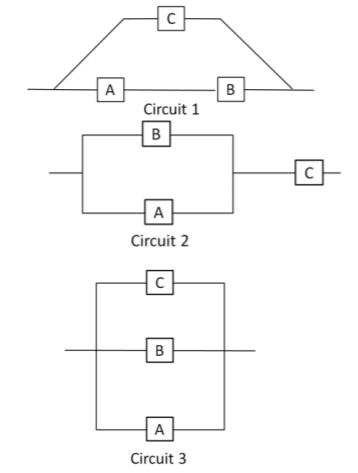
\includegraphics[width=\columnwidth]{solutions/2016/june/118/Figures/circuits.png}
    \caption{Figure}
    \label{fig:fig_label}
\end{figure}
%
\solution
For $q_1$, the truth table
\begin{table}[h]
    \centering
    \begin{tabular}{|c|c|c|c|}
    \hline
         $A$ & $B$ & $C$ & $(AB) + C$ \\
         \hline
         1 &1  & 0 &1\\\hline
         1&1&1&1\\\hline
         0&1&1&1\\\hline
         0&0&1&1\\\hline
         1&0&1&1\\
    \hline
    \end{tabular}
    \caption{Circuit 1 working}
    \label{june2016-118:tab:my_label}
\end{table}
Multiplying and adding probability for each case of $q_1$ gives us the value of $q_1$ as
\begin{align}
    q_1 = p^3-2p^2+1
\end{align}
For $q_2$, the truth table
\begin{table}[h]
    \centering
    \begin{tabular}{|c|c|c|c|}
    \hline
         $A$ & $B$ & $C$ & $(A+B)C$ \\
         \hline
         1&1&1&1\\ \hline
         1&0&1&1\\\hline
         0&1&1&1\\
    \hline
    \end{tabular}
    \caption{Circuit 2 working}
    \label{june2016-118:tab:table2}
\end{table}
Multiplying and adding probability for each case of $q_2$ gives us the value of $q_2$ as
\begin{align}
    q_2 = p^3-p^2-p+1
\end{align}
For $q_3$, the truth table
\begin{table}[h]
    \centering
    \begin{tabular}{|c|c|c|c|}
    \hline
         $A$ & $B$ & $C$ & $A + B + C$ \\
         \hline
         1&0&0&1\\\hline
         0&1&0&1\\\hline
         0&0&1&1\\\hline
         1&1&0&1\\\hline
         1&0&1&1\\\hline
         0&1&1&1\\\hline
         1&1&1&1\\
    \hline
    \end{tabular}
    \caption{Circuit 3 working}
    \label{june2016-118:tab:table3}
\end{table}
Multiplying and adding probability for each case of $q_3$ gives us the value of $q_3$ as
\begin{align}
    q_3 = 1-p^3
\end{align}
%%
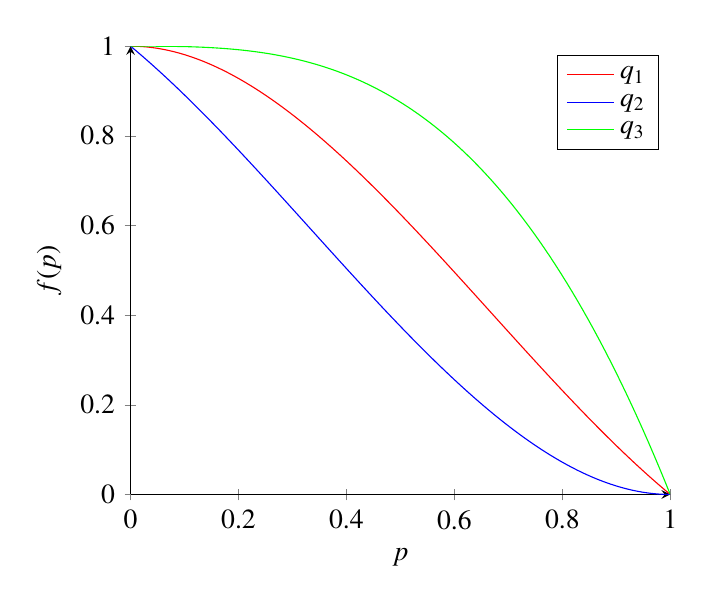
\begin{tikzpicture}
\begin{axis}[
    axis lines = left,
    xlabel = $p$,
    ylabel = {$f(p)$},
]
\addplot [
    domain=0:1, 
    samples=100, 
    color=red,
]
{x^3-2*x^2+1};
\addlegendentry{$q_1$}
\addplot [
    domain=0:1, 
    samples=100, 
    color=blue,
    ]
    {x^3-x^2-x+1};
\addlegendentry{$q_2$}
\addplot [
    domain=0:1, 
    samples=100, 
    color=green,
]
{1-x^3};
\addlegendentry{$q_3$}
\end{axis}
\end{tikzpicture}
\begin{align}
    \therefore q_3>q_1>q_2
\end{align}
Hence \textbf{Option 1} is correct
\end{enumerate}

\section{Elementary Probability}
\renewcommand{\theequation}{\theenumi}
\renewcommand{\thefigure}{\theenumi}
\renewcommand{\thetable}{\theenumi}
\begin{enumerate}[label=\thesection.\arabic*.,ref=\thesection.\theenumi]
\numberwithin{equation}{enumi}
\numberwithin{figure}{enumi}
\numberwithin{table}{enumi}

\item There are 3 red socks, 4 green socks and 3 blue socks.You choose 2 socks.The probability that they are of the same colour is

\begin{enumerate}
\begin{multicols}{4}
\setlength\itemsep{2em}

\item $\dfrac{1}{5}$
\item $\dfrac{7}{30}$
\item $\dfrac{1}{4}$
\item $\dfrac{4}{15}$

\end{multicols}
\end{enumerate}
\solution
Let $X_i \in \cbrak{1, 2, 3}$ represent the $i^{th}$ draw, where 1, 2, 3 correspond to the colour of socks drawn as Red, Blue and Green respectively
\begin{table}[ht]
\centering 
\caption{}
\begin{tabular}{|c|c|c|c|}
\hline
           & $X_1 = 1$ & $X_1 = 2$ & $X_1 = 3$\\
\hline
$X_2 = 1$  & 6/90      & 12/90     & 9/90  \\
\hline
$X_2 = 2$  & 12/90      & 12/90    & 12/90  \\
\hline
$X_2 = 3$  & 9/90      & 12/90    & 6/90  \\
\hline
\end{tabular}
\label{cond/1/table}
\end{table}
  
TABLE  \ref{cond/1/table} represents all the possibilities of choosing socks one by one.
  
 
The probability that the two socks drawn are of the same colour(by substituting values from table \ref{cond/1/table})
 \begin{align}
     &= \Pr\brak{X_1 = X_2} \\
     &= \sum_{i = 1}^3 \Pr\brak{X_2 = i | X_1 = i}\Pr\brak{X_1 = i}\\
     &= \dfrac{6}{90} +\dfrac{12}{90} + \dfrac{6}{90}\\
     &= \dfrac{4}{15}
 \end{align}
 So the correct option is (D)
%
\item A box contains 40 numbered red balls and 60 numbered black balls. From the box, balls are drawn one by one at random without replacement till all the balls are drawn. The probability that the last ball drawn is black equals \dots
Now, this problem is equivalent to the problem where we have to arrange 40 distinct R's and 60 distinct B's such that, a B should come at last. So,
the desired probability is given by 
\begin{multline}
\frac{\text{(placing a B at last)} \times \text{(arranging other letters)}}{\text{arranging 100 letters}} \\  = \frac{60 \times 99! }{100!}
 = \frac{3}{5} \label{cond/2/Eq:4}
\end{multline}


\item An experiment consists of two papers.paper1 and paper2.The probability of failing in paper 1 is .3 and that in paper 2 is .2.Given that a student has failed in paper 2,the probability of failing in paper 1 is .6.The probability of student failing in both is\\
\begin{enumerate}
    \setlength\itemsep{2em}
\item .5 
\item .18 
\item .12 
\item .06 
\end{enumerate}
%
\solution
\begin{table}[!ht]
    \centering
    \begin{tabular}{|c|c|c|}
    \hline
         &Description  & Probability \\
         \hline
         0&failure & $\pr{X=0} = 0.3$\\
         \hline
         1&success & $\pr{Y=0} = 0.2$\\
         \hline
         X&Paper 1 & $\pr{X=0|Y=0} = 0.6$\\
         \hline
         Y&Paper 2 & \\
         \hline
    \end{tabular}
    \caption{Description}
    \label{table:axioms/3}
\end{table}
%
Table \ref{table:axioms/3} summarises the given information.  The desired probability is
%
    \begin{align}
        \pr{X=0,Y=0} &= \pr{X=0|Y=0}\pr{Y=0}\\ 
        &=.12
       \end{align}

%
\item An urn contains 5 red balls and 5 black balls.In the first draw, one ball is picked at random and discarded without noticing its colour.The probability to get a red ball in the second draw is 
\begin{enumerate}
    \begin{multicols}{4}
    \setlength\itemsep{2em}
    
    \item $\dfrac{1}{2}$
    \item $\dfrac{4}{9}$
    \item $\dfrac{5}{9}$
    \item $\dfrac{6}{9}$
    \end{multicols}
    \end{enumerate}    
%
\solution
Let $X_i \in \cbrak{0,1}$ represent the $i^{th}$ draw where 1 denotes a red ball being drawn.

\begin{table}[h]
\centering 
\begin{tabular}{|c|c|c|}
\hline
           & $X_1 = 0$ & $X_1 = 1$\\
\hline
$X_2 = 0$  & 4/18      & 5/18  \\
\hline
$X_2 = 1$  & 5/18      & 4/18  \\
\hline
\end{tabular}
\caption{The probabilities of all possible cases when two balls are drawn one by one from the urn.}
\label{axioms/4/table:}
\end{table}
 
From Table \ref{axioms/4/table:},

\begin{align}
    \pr{X_2 = 1} &= \pr{X_2 = 1,X_1 = 0} \nonumber \\
    & \quad +\pr{X_2 = 1,X_1 = 1} \\
                 &=\frac{5}{18}+\frac{4}{18} \\
                 &= \frac{1}{2}
\end{align}
The required option is (A).
%
%
\item A sample of size $n =2$ is drawn from a population of size $N=4$ using probability proportional to size without replacement scheme , Where the probabilities proportional to size are
\begin{table}[h!]
\resizebox{\columnwidth}{0.6cm}{%
  \begin{tabular}{|c|c|c|c|c|}
    \hline
    i: & 1 & 2 & 3 & 4\\
    \hline
    $p_{i}$ & 0.4 & 0.2 & 0.2 & 0.2\\
    \hline
  \end{tabular}%
} 
   \caption*{Table : Probability vs Size}
\end{table}  
The probability of inclusion of unit (1) in the sample is 
\begin{enumerate}
\begin{multicols}{4}
\setlength\itemsep{2em}
\item $0.4$
\item $0.6$
\item $0.7$
\item $0.75$
\end{multicols}
%

\end{enumerate}
%
\solution
Let $P_{i}(j)$ represent the probability for selecting unit (j) as second unit after selecting  unit (i) 
\begin{align}
    P_{i}(j)&=\frac{p_{j}}{1-p_{i}}
    \label{2019-58:eq:eq2}
\end{align}
Let  $\pr{i,j}$ be probability of selecting sample \{i,j\} ,using \eqref{eq:eq2}  is 
\begin{align}
    \pr{i,j}&=P_{i}(j)+P_{j}(i)
    \\
    &=\brak{p_{i}\times \frac{p_{j}}{1-p_{i}}} + \brak{p_{j}\times \frac{p_{i}}{1-p_{j}}}
    \label{2019-58:eq:eq3}
\end{align}
Total samples(Size $n=2$)are 
\definecolor{green}{RGB}{0 150, 22}
\definecolor{Red}{RGB}{200,60,40}
\definecolor{mycolor}{RGB}{0, 60, 240}
\begin{table}[h!]
\resizebox{\columnwidth}{0.95cm}{%
  \begin{tabular}{|c ||c ||c |c | c| c| c|}
    \hline
    \textcolor{green}{Case }&  \textcolor{Red}{1} & \textcolor{Red}{2} & \textcolor{Red}{3} & \textcolor{Red}{4} & \textcolor{Red}{5} & \textcolor{Red}{6}\\
    \hline
    \textcolor{green}{Sample(size $n=2$)} & \textcolor{mycolor}{\brak{1,2}} & \textcolor{mycolor}{\brak{1,3} }& \textcolor{mycolor}{\brak{1,4} }& \textcolor{mycolor}{\brak{2,3}} & \textcolor{mycolor}{\brak{2,4}}& \textcolor{mycolor}{\brak{3,4}}\\
    \hline
  \end{tabular}%
} 
  \caption{ list of samples}
  \label{2019-58:tab:label1_test}
\end{table}
Let $P_{i}$ be the probability of inclusion of unit (i) in the sample(size $n=2$),Now i will calculate $P_{1}$ ,Favourable cases for inclusion of unit(1) are case (\textcolor{red}{1,2,3}),So
\begin{align}
    P_{1}&=\pr{1,2} +\pr{1,3}+\pr{1,4}
\end{align}
using \eqref{2019-58:eq:eq3} and $p_{i}$ from question ,
\begin{align}
    P_{1}&=\frac{7}{30} + \frac{7}{30} + \frac{7}{30}
    \\
    &=0.7
\end{align}
Therefore Option (3) is correct.

%
%
\item There are two boxes. Box-$1$ contains $2$ red balls and $4$ green balls. Box-$2$ contains $4$ red balls and $2$ green balls. A box is selected at random and a ball is chosen randomly from the selected box. If the ball turns out to be red, what is the probability that Box-$1$ had been selected?
%
\solution
Box-$1$ has $2$ red balls and $4$ green balls.\\
Box-$2$ has $4$ red balls and $2$ green balls.\\
Let $B \in \{1,2\} $ represent a random variable where $1$ represents selecting box-$1$ and $2$ represents selecting box-$2$.
\begin{table}[h!]
\resizebox{\columnwidth}{!}
{ 
\begin{tabular}{|c|c|c|}
\hline
Event & definition & value\\
\hline
$ \pr{B=1} $ & Probability of selecting  & $\frac{1}{2}$\\
&Box-$1$ & \\
\hline
$ \pr{B=2} $ & Probability of selecting & $\frac{1}{2}$ \\
& Box-$2$& \\
\hline
$\pr{R=1|B=1}$ & Probability of drawing &  $\frac{1}{3}$   \\
&  red ball from Box-$1$ &\\
\hline
$\pr{G=1|B=1}$ & Probability of drawing &  $\frac{2}{3}$   \\
&  green ball from Box-$1$ &\\
\hline
$\pr{R=1|B=2}$ & Probability of drawing &  $\frac{2}{3}$   \\
&  red ball from Box-$2$ &\\
\hline
$\pr{G=1|B=2}$ & Probability of drawing &  $\frac{1}{3}$   \\
&  green ball from Box-$2$ &\\
\hline
\end{tabular}
}
\caption{Table 1} 
\label{dec2016-49:tab:1}
\end{table}
From Baye's theorem
\begin{align}
\pr{R=1}&=\pr{R=1|B=1} \times \pr{B=1} \notag \\
 & +\pr{R=1|B=2} \times \pr{B=2}  \label{dec2016-49:1}
 \end{align}
Substiting values from table \eqref{dec2016-49:tab:1} in \eqref{dec2016-49:1}
\begin{align}
\pr{R=1} &=\frac{1}{2} \label{dec2016-49:2} \\
\pr{(R=1)(B=1)}&=\pr{R=1|B=1}\notag \\
&  \times \pr{B=1} \\ 
&= \frac{1}{6}  \label{dec2016-49:3}
\end{align}
We need to find $\pr{B=1|R=1}$ \\
\begin{align}
\pr{B=1|R=1} &= \frac{\pr{(R=1 ) (B=1)}}{\pr{R=1}} \\
&=\frac{1}{3}
\end{align}
 $\therefore$ The desired probability that box-$1$ is selected $= \frac{1}{3}$ \\
 
%
\item An urn has 3 red and 6 black balls. Balls are drawn at random one by one without replacement. The probability that second red ball appears on fifth draw is: \\
\begin{enumerate}
    \item $\frac{1}{9!}$
    \newline
    \item $\frac{4!}{9!}$
    \newline
    \item $4\brak{\frac{6!4!}{9!}}$
    \newline
    \item $\frac{6!4!}{9!}$
\end{enumerate}
%
%
\solution
 To obtain a second red ball at the fifth draw, the first 4 trials should involve drawing only 1 red ball out of the 3 and 3 black balls out of the 6. Probability of this happening:
 \begin{align}
  \frac{\comb{3}{1}\comb{6}{3}}{\comb{9}{4}}
     \end{align}
The probability of the fifth ball turning out to be red is:
\begin{align}
    \frac{\comb{2}{1}}{\comb{5}{1}}
\end{align}
By Multiplication rule, total probability:
\begin{align}
    \frac{\comb{3}{1}\comb{6}{3}\comb{2}{1}}{\comb{5}{1}\comb{9}{4}}
    = \frac{3!\times 6!\times2!\times4!\times4!\times5!}{2!\times3!\times3!\times5!\times9!}\\ 
    =4\brak{\frac{4!6!}{9!}}
\end{align}

%


\end{enumerate}

\section{Random Variables}
\renewcommand{\theequation}{\theenumi}
\renewcommand{\thefigure}{\theenumi}
\renewcommand{\thetable}{\theenumi}
\begin{enumerate}[label=\thesection.\arabic*.,ref=\thesection.\theenumi]
\numberwithin{equation}{enumi}
\numberwithin{figure}{enumi}
\numberwithin{table}{enumi}

\item Suppose the random varible $X$ has the following probability density function
\begin{align}
f(x)=
\begin{cases}
\alpha(x-\mu)^{\alpha-1}e^{-(x-\mu)^\alpha} &x>\mu\\
0 &x\leq\mu,
\end{cases}
\end{align}
Where $\alpha>0, -\infty<\mu<\infty$. Which of the following statements are correct? The Hazard function of $X$ is
\begin{enumerate}[label=\alph*)]
\item an increasing function for all $\alpha>0$
\item a decreasing function for all $\alpha>0$
\item an increasing function for some $\alpha>0$
\item a decreasing function for some $\alpha>0$
\end{enumerate}
%
\solution

The Hazard function of $X$,
\begin{align}
\lambda(X) = \frac{f(x)}{S(x)} \label{var/1/eq:1}
\end{align}
where $S(x)$ is the survival function given by,
\begin{align}
S(x) = P(X \geq x) = 1-F(x) = \int_{x}^{\infty}f(t)dt
\end{align}
\begin{lemma}
\begin{align}
S(x)=
\begin{cases}
e^{-(x-\mu)^\alpha} &x>\mu\\
1 &x\leq\mu
\end{cases}
\end{align}
\end{lemma}
\begin{proof}

\begin{align}
\int f(t)dt=\int \alpha(t-\mu)^{\alpha-1}e^{-(t-\mu)^\alpha}dt\\
=-e^{-(t-\mu)^\alpha} + C
\end{align}
If $x>\mu$, 
\begin{align}
S(x) = \int_{x}^{\infty} \alpha(t-\mu)^{\alpha-1}e^{-(t-\mu)^\alpha}dt\\
=-e^{-(t-\mu)^\alpha}]_{x}^{\infty}\\
=e^{-(x-\mu)^{\alpha}} \label{var/1/eq:2}
\end{align}
If $x\leq\mu$,
\begin{align}
S(x) = \int_{x}^{\mu}f(t)dt + \int_{\mu}^{\infty}f(t)dt\\
     = 0 + e^{-(\mu-\mu)^{\alpha}}\\
     =1 \label{var/1/eq:3}
\end{align}
From \eqref{var/1/eq:2} and \eqref{var/1/eq:3}, we get $S(x)$ as,
\begin{align}
S(x)=
\begin{cases}
e^{-(x-\mu)^\alpha} &x>\mu\\
1 &x\leq\mu \label{var/1/eq:4}
\end{cases}
\end{align}
\end{proof}
From \eqref{var/1/eq:1} and \eqref{var/1/eq:4}, we get
\begin{align}
\lambda(x) = 
\begin{cases}
\alpha(x-\mu)^{\alpha-1} &x>\mu\\
0 &x\leq\mu \label{var/1/eq:5}
\end{cases}
\end{align}
So,\\ if $\alpha>1$, $\lambda(x)$ is an increasing function
\begin{figure}[htp]
    \centering
    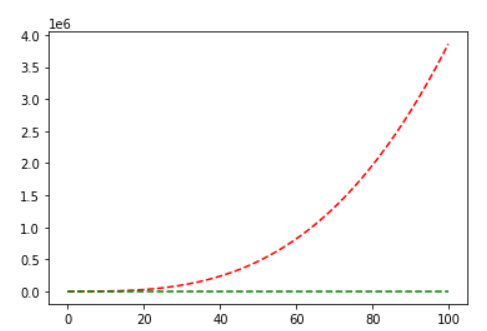
\includegraphics[width=\columnwidth]{variable/solutions/1/alphagrt1.png}
    \caption{$\alpha=2$ for red. $\alpha=1$ for green, $\mu=1$ for both}
    \label{var/1/fig:grt1}
\end{figure}
and\\ if $0<\alpha<1$, $\lambda(x)$ is a decreasing function
\begin{figure}[htp]
    \centering
    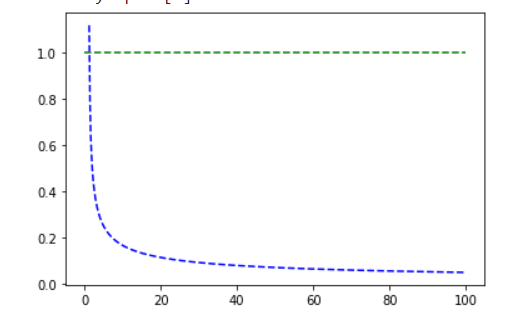
\includegraphics[width=\columnwidth]{variable/solutions/1/alphales1.png}
    \caption{$\alpha=0.5$ for blue. $\alpha=1$ for green, $\mu=1$ for both}
    \label{var/1/fig:les1}
\end{figure}
and\\ for $\alpha=1$, $\lambda(x)=1$, a constant function.\\
So, for some values of $\alpha$, it is increasing, for some it is decreasing function\\
\textbf{Therefore, answer is (C) and (D)}




\item Consider the function \textit{f(x)} defined as \textit{f(x)} = \textit{ce$^{-x^{4}}$}, $\textit{x} \in R$ . For what value of \textit{c} is \textit{f} a probability density function?\\
\begin{enumerate}
    \item $\displaystyle\frac{2}{\Gamma(1/4)}$\\\label{june/2019/52/option 1}
    \item $\displaystyle\frac{4}{\Gamma(1/4)}$\\
    \item $\displaystyle\frac{3}{\Gamma(1/3)}$\\
    \item $\displaystyle\frac{1}{4\Gamma(4)}$
\end{enumerate}
%
\solution
Consider a continuous random variable X so that the function \textit{f} can be probability density function if and only if it satisfies the condition 
\begin{align}
    \int_{-\infty}^{\infty}f_{X}(u)du = 1 \label{2019/52/equation 1}
\end{align}
Hence by applying the \eqref{2019/52/equation 1} for the function \textit{f} we get
\begin{align}
    \int_{-\infty}^{\infty}ce^{-u^{4}}du = 1\\
    2c\int_{0}^{\infty}e^{-u^{4}}du = 1\label{2019/52/equation 2}\\
    2c\int_{0}^{\infty}e^{-t}\frac{dt}{4t^{\frac{3}{4}}} = 1\\
    \frac{c}{2}\int_{0}^{\infty}e^{-t}t^{-\frac{3}{4}}dt = 1\label{2019/52/equation 3}
\end{align}
We know that gamma function for any real positive $\alpha$
\begin{align}
    \Gamma(\alpha) = \int_0^\infty x^{\alpha - 1} e^{-x} dx \label{2019/52/gammafunction}
\end{align}
Hence by using \eqref{2019/52/gammafunction} in \eqref{2019/52/equation 3} we get
\begin{align}
    \frac{c}{2}\Gamma(1/4) = 1\\
    c=\frac{2}{\Gamma(1/4)}
\end{align}
Hence $c = \displaystyle\frac{2}{\Gamma(1/4)}$ and option \eqref{2019/52/option 1} is correct.\newline\newline
The CDF of \textit{f} by using \eqref{2019/52/gammafunction} we get
\begin{align}
    F_{X}(x) &= \int_{0}^{x}f(u)du\\
             &= \frac{2}{\Gamma(\frac{1}{4})}\int_{0}^{x}e^{-u^{4}}du\\
             &= \frac{2}{4\Gamma(\frac{1}{4})}\int_{0}^{x^{4}}e^{-t}{t^{\frac{-3}{4}}}dt\\
             &= \frac{1}{2\Gamma(\frac{1}{4})}\int_{0}^{x^{4}}e^{-t}{t^{\frac{-3}{4}}}dt\\
             &= \frac{1}{2\Gamma(\frac{1}{4})}\brak{\Gamma\brak{\frac{1}{4}}-\Gamma\brak{\frac{1}{4},x^{4}}}\\
             &= \frac{1}{2\Gamma(\frac{1}{4})}\gamma\brak{\frac{1}{4},x^{4}}
\end{align}

\item Let X and Y be i.i.d random variables uniformly distributed on (0,4).Then \pr{X>Y|X<2Y} is
\begin{enumerate}
    \item 1/3
    \item 5/6
    \item 1/4
    \item 2/3
\end{enumerate}
\solution

The PDF is given by
\begin{align}
   &f_X (x)=f_Y (x)=\nonumber \begin{cases}
         \frac{1}{4}, &\text{if 0 \(< x <\) 4}\\
         0, &\text{otherwise}\\
   \end{cases} 
\end{align}    
The CDF is given by
\begin{align}
   \nonumber& F(x)=\int_{-\infty}^{x} f(x)dx \\ \nonumber
   &F_X (x)=F_Y (x)=\nonumber \begin{cases}
          0, & x\leq 0\\
         \frac{x}{4}, &\text{if 0 \(< x <\) 4}\\
          1, &x\geq4\\
   \end{cases}    
\end{align}
Using definition of conditional probability 
\begin{align}
    &\pr{X>Y|X<2Y}=\frac{\pr{Y < X< 2Y}}{\pr{X<2Y}} \label{eqn1}
\end{align}
Now finding \pr{X<2Y}
\begin{align}
    &\pr{X<2y}=F_X (2y)\\
    \implies& \pr{X<2Y}=\int_{-\infty}^{\infty} f_Y(x) \times F_X (2x)dx\\
    \implies& \pr{X<2Y}=\int_{0}^{2} \frac{x}{8}dx +\int_{2}^{4}\frac{1}{4}dx\\
    \implies& \pr{X<2Y}=\frac{3}{4}=0.75 \label{eqn2}
\end{align}
Now to find \pr{Y<X<2Y}
\begin{align}
    &\pr{y<X<2y}=F_X (2y)- F_X (y) \\
    \implies &\pr{Y<X<2Y}\\ \nonumber 
    &=\int_{-\infty}^{\infty} f_Y (x)( F_X (2x)- F_X(x))dx \\
   \implies &\int_{0}^{2}\frac{1}{4}\brak{\frac{x}{2}-\frac{x}{4}} dx +\int_{2}^{4}\frac{1}{4}\brak{1-\frac{x}{4}} dx\\
   \implies &\pr{Y<X<2Y}=\frac{1}{4}=0.25 \label{eqn3}
\end{align}
Now using \eqref{eqn1},\eqref{eqn2} and \eqref{eqn3}
\begin{align}
    \pr{X>Y|X<2Y}=\frac{1/4}{3/4}=\frac{1}{3}
\end{align}
Hence final solution is option 1) or 1/3 
%
\item Suppose $X$ is a positive random variable with the following probability density function,
\begin{align*}
f(x) = (\alpha x^{\alpha -1} + \beta x^{\beta-1} ) e^{-x^{\alpha}-x^{\beta}} ; x>0
\end{align*}
for $ \alpha >0, \beta >0$.
Then the hazard function of $X$ for some choices of $\alpha$ and $\beta$ can be
\begin{enumerate}
    \item an increasing function.
    \item a decreasing function.
    \item a constant function.
    \item a non monotonic function
\end{enumerate}
%
\solution


CDF of $X$, 
\begin{align}
    F(x) &=  \int_{-\infty}^xf(t)dt \\
    &= \int_{0}^xf(t)dt \hspace{1cm} \text{as } x>0\\
    &= \int_{-\infty}^t\left((\alpha t^{\alpha -1} + \beta t^{\beta-1} ) \times e^{-t^{\alpha}-t^{\beta}}\right)dt \\
    &= -e^{-t^{\alpha}-t^{\beta}} \Big|_0^x\\
    &= 1-e^{-x^{\alpha}-x^{\beta}}
\end{align}
Hazard function,
\begin{align}
    h(x) &= \frac{f(x)}{1-F(x)} \\
    &= \alpha x^{\alpha -1} + \beta x^{\beta-1} \\
    h^{\prime}(x) &= \alpha(\alpha -1) x^{\alpha -2} + \beta(\beta-1) x^{\beta-2}\\
     h^{\prime}(x) &= 
         \begin{cases}
    0 & \alpha=\beta=1 \\
    >0 & \text{otherwise}\\
    \end{cases}
    \end{align}
    Thus $h(x)$ can be either constant function or an increasing function.
    
    \begin{figure}[h]
    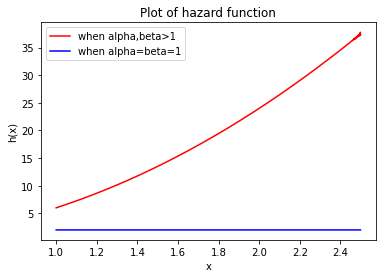
\includegraphics[width=\columnwidth]{solutions/2018/dec/118/figures/plot.png}
    \end{figure}
     From the above figure, it is verified that $h(x)$ can be either constant function or an increasing function.\\
       Correct options are 1,3.





%
\item Suppose the random variable X has the following probability density funtion 
\begin{align}
    f(x)=\begin{cases}\alpha\brak{x-\mu}^{\alpha -1}e^{-\brak{x-\mu}^\alpha};&x>\mu\\
                        0                               &x\leq\mu    
    \end{cases}\nonumber
\end{align}
where $\alpha>0,-\infty <\mu<\infty$. Which of the following are correct? The hazard function of $X$ is
\begin{enumerate}
    \item an increasing function for all $\alpha>0$
    \item a decreasing function for all $\alpha >0$
    \item an increasing function for some $\alpha>0$
    \item a decreasing function for some $\alpha>0$
\end{enumerate}
%
\solution

\newcommand{\Integral}[2]{solutions/2017/june/118/figures/\ensuremath{\int\limits_{#1}^{#2}}}
For the random variable $X$, the CDF is
\begin{align}
    F(x)&=\Integral{0}{x}f(y)dy\\
        &=\Integral{0}{\mu}0 dy +\Integral{\mu}{x}\alpha\brak{y-\mu}^{\alpha -1}e^{-\brak{y-\mu}^\alpha}\\
        &=0 -e^{-\brak{y-\mu}^\alpha}\Big|_{\mu}^{x}\\
        &=1-e^{-\brak{x-\mu}^{\alpha}}
\end{align}
For X, the hazard function $H(y)$ is defined as
\begin{align}
    H(y)&=\frac{f(y)}{1-F(y)}\nonumber\\
    \implies H(y)&=\begin{cases}\frac{\alpha\brak{y-\mu}^{\alpha -1}e^{-\brak{y-\mu}^\alpha}}{1-\brak{1-e^{-\brak{y-\mu}^{\alpha}}}};&y>\mu\\
                        0                               &y\leq\mu   
    \end{cases}\nonumber\\
    &=\begin{cases}\alpha\brak{y-\mu}^{\alpha -1};&y>\mu\\
                        0                            &y\leq\mu   
    \end{cases}\nonumber
\end{align}
Differentiating $H(y)$ w.r.t. $y$
\begin{align}
    H'(y)&=\begin{cases}\alpha\brak{\alpha - 1}\brak{y-\mu}^{\alpha -2};&y>\mu\\
                        0                            &y\leq\mu   
    \end{cases}\nonumber
\end{align}
When $y\leq \mu$ then $H'(y)$ is $0$. When $y>\mu$ then $\brak{y-\mu}^{\alpha -2}$ is positive. This implies that the sign for $H'(y)$ for $y>\mu$ is decided by the sign of $\alpha\brak{\alpha -1}$.
\begin{align}
    \alpha\brak{1-\alpha}<0
    \implies 0<\alpha<1\nonumber\\
    \alpha\brak{1-\alpha}>0\implies \alpha>1 &&\text{(ignoring $\alpha<0$)}\nonumber
\end{align}
$\therefore$ The Hazard function of $X$ is decreasing when $\alpha \in \brak{0,1}$ and increasing when $\alpha \in \brak{1,\infty}$
\vspace{0.5cm}\centering \boxed{\solution{\text{Options 3, 4}}}
% \iffalse
% \begin{figure}[h!]
%     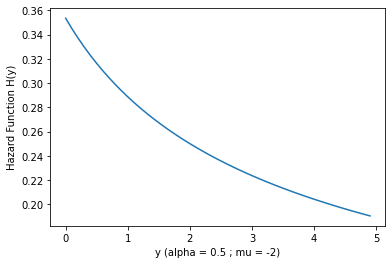
\includegraphics[width = \columnwidth]{solutions/2017/june/118/figures/Figure-1.png}
%     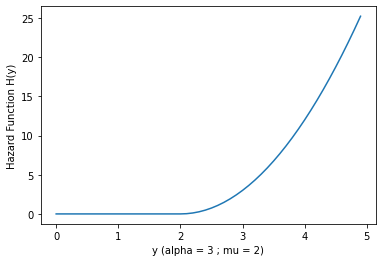
\includegraphics[width = \columnwidth]{solutions/2017/june/118/figures/Figure-2.png}
% \end{figure}
% \fi
\begin{figure}[h]
    \centering
    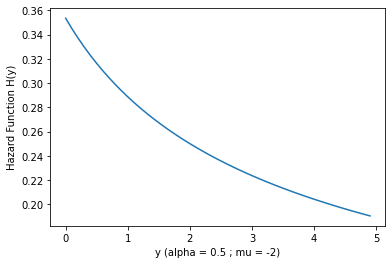
\includegraphics[width=\columnwidth-50pt]{solutions/2017/june/118/figures/Figure-1.png}
    \caption{Decreasing Hazard Function}
    \label{june/2017/118/fig:my_label1}
\end{figure}
\begin{figure}[h]
    \centering
    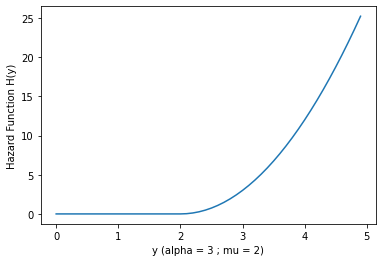
\includegraphics[width=\columnwidth-50pt]{solutions/2017/june/118/figures/Figure-2.png}
    \caption{Increasing Hazard Function}
    \label{june/2017/118/fig:my_label2}
\end{figure}

%
%
\item Let $X$ be a random variable with a certain non-degenerate distribution. Then identify the correct statements
\begin{enumerate}
    \item If $X$ has an exponential distribution then $median\brak{X}<E\brak{X}$
    \item If $X$ has a uniform distribution on an interval $[a,b]$, then $E\brak{X}<median\brak{X}$
    \item If $X$ has a Binomial distribution then $V\brak{X}<E\brak{X}$
    \item If $X$ has a normal distribution, then $E\brak{X}<V\brak{X}$
\end{enumerate}
%
\solution
Expected value\brak{E\brak{X}}:
It is nothing but weighted average
Median\brak{median\brak{X}}:
It is the value separating the higher half from the lower half of a data sample
Variance\brak{V\brak{X}}:
It is the expectation of the squared deviation of a random variable from its mean
\begin{enumerate}
    \item Let's consider $X$ has an exponential distribution.
    \begin{align}
        X \sim Exp\brak{\lambda}
    \end{align}
    where $\lambda$ is rate parameter.
    
    Probability function of exponential distribution,
    \begin{align}
        f_X\brak{x}=
        \begin{cases}
            \lambda e^{-\lambda x} & x\geq0\\
            0 & x<0
        \end{cases}
    \end{align}
    The expected value of $X \sim Exp\brak{\lambda}$,
    \begin{align}
        E\brak{X}=\frac{1}{\lambda}
    \end{align}
    The median of $X \sim Exp\brak{\lambda}$,
    \begin{align}
        median\brak{X}=\frac{\ln{2}}{\lambda}
    \end{align}
    \begin{align}
        \ln{2}<1\\
        \frac{\ln{2}}{\lambda}<\frac{1}{\lambda}\\
         median\brak{X}<E\brak{X}
    \end{align}
    Hence, option $1$ is correct.
    
    \item Let's consider $X$ has a uniform distribution in interval $[a,b]$,
    \begin{align}
        X \sim U\brak{a,b}
    \end{align}
    where,
    $a=$ lower limit
    
    $b=$ upper limit
    
    Probability function of uniform distribution,
    \begin{align}
        f_X\brak{k}=
        \begin{cases}
            \frac{1}{b-a} & a\leq x\leq b\\
            0 & x < a, x > b
        \end{cases}
    \end{align}
    The expected value of $X \sim U\brak{a,b}$,
    \begin{align}
        E\brak{X}=\frac{1}{2}\brak{a+b}
    \end{align}
    The median of $X \sim U\brak{a,b}$,
    \begin{align}
        median\brak{X}=\frac{1}{2}\brak{a+b}
    \end{align}
    \begin{align}
        E\brak{X}=median\brak{X}
    \end{align}
    Hence, option $2$ is incorrect.
    
    \item Let's consider $X$ has a binomial distribution,
    \begin{align}
        X \sim B\brak{n,p}
    \end{align}
    where,
    $n=$ no. of trails
    
    $p=$ success parameter
    
    Probability function of binomial distribution,
    \begin{align}
        f_X\brak{k}=
        \begin{cases}
            {^n C_k}p^k(1-p)^{n-k} & 0\leq k\leq n\\
            0 & otherwise
        \end{cases}
    \end{align}
    The expected value of $X \sim B\brak{n,p}$,
    \begin{align}
        E\brak{X}=np
    \end{align}
    The variance of $X \sim B\brak{n,p}$,
    \begin{align}
        V\brak{X}=\sigma^2=n p(1-p)
    \end{align}
    \begin{align}
        1-p\leq1\\
        n p(1-p)\leq n p\\
        V\brak{X}\leq E\brak{X}
    \end{align}
    Hence, option $3$ is incorrect.
    
    \item Let's consider $X$ has a normal distribution,
    \begin{align}
        X \sim N\brak{\mu,\sigma^2}
    \end{align}
    where,
    $\mu=$ mean of distribution
    
    $\sigma^2=$ variance
    
    Probability function of normal distribution,
    \begin{align}
        f_X\brak{k}=\frac{1}{\sigma\sqrt{2\pi}}e^{-\brak{\frac{x-\mu}{2\sigma}}^2}
    \end{align}
    The expected value of $X \sim N\brak{\mu,\sigma^2}$,
    \begin{align}
        E\brak{X}=\mu
    \end{align}
    The variance of $X \sim N\brak{\mu,\sigma^2}$,
    \begin{align}
        V\brak{X}=\sigma^2
    \end{align}
    $E\brak{X}$ and $V\brak{X}$ are user defined. So, they can take any value.
    
    Hence, option $4$ is incorrect.
    \end{enumerate}
    
%
\item A fair coin is tossed repeatedly. Let $X$ be the number of tails before the first heads occurs. Let $Y$ denote the number of tails between the first and second heads. Let $X+Y = N$. Then which of the following are true?
\begin{enumerate}
    \item X and Y are independent random variables with
    {\footnotesize
    \begin{align}
        \pr{X = k} = \pr{Y = k} =
        \begin{cases}
            2^{-(k+1)} & k=0,1,2 \ldots
            \\
            0 & otherwise
        \end{cases}
    \end{align}
    }
    \item $N$ has a probability mass function given by
    {\small
     \begin{align}
        \pr{N = k} =
        \begin{cases}
            (k-1)2^{-k} & k=2,3,4 \ldots
            \\
            0 & otherwise
        \end{cases}
    \end{align}
    }
    \item Given $N = n$, the conditional distribution of X and Y are independent
    \item Given $N = n$
     \begin{align}
        \pr{X = k} =
        \begin{cases}
            \frac{1}{n+1} & n=0,1,2 \ldots
            \\
            0 & otherwise
        \end{cases}
    \end{align}
\end{enumerate}
%

\item Assume that $X\sim Binomial(n, p)$ for some $n\geq 1$ and $0<p<1$
and $Y\sim poisson(\lambda)$for some $\lambda > 0$.Suppose E[X]=E[Y].Then
\begin{enumerate}
    \item $var(X)=Var(Y)$\\
    \item $var(X)<Var(Y)$\\
    \item $var(Y)<Var(X)$\\
    \item $Var(X)$ may be larger or smaller than $Var(Y)$ depending on the values of n,p and $\lambda$
\end{enumerate}
%
%
\solution
For the random variable $$X\sim Binomial(n, p)$$
As we know,
\begin{align}
E[X]&=np\\
Var(X)&=np(1-p) \label{june/2015/53a}
\end{align}
for the random variable $$Y\sim poisson(\lambda)$$
As we know,
\begin{align}
E[Y]&=\lambda\\
Var(Y)&=\lambda \label{june/2015/53b}
\end{align}
given that,
\begin{align}
E[X]&=E[Y]\\
np&=\lambda \label{june/2015/53c}
\end{align}
from \eqref{june/2015/53a},
\begin{align}
Var(X)&=np(1-p)
\end{align}
using \eqref{june/2015/53c},
\begin{align}
Var(X)&=\lambda(1-p)
\end{align}
\begin{table}[ht]
\caption{Mean and Variance for random variables X and Y}
\begin{center}
    \begin{tabular}{|c|c|c|}
    \hline
     & $X$&$Y$\\
    \hline
    E& $\lambda$& $\lambda$\\
    \hline
     $var$& $\lambda(1-p)$ & $\lambda$\\
    \hline
    \end{tabular}
\end{center} 
\label{june/2015/53tab:1}
\end{table}
using \eqref{june/2015/53b},
\begin{align}
Var(X)&=Var(Y)(1-p)\\
\frac{Var(X)}{Var(Y)}&= 1-p
\end{align}
as,
\begin{align}
1-p &<1\\
\frac{Var(X)}{Var(Y)}&<1\\
Var(X) &< Var(Y)
\end{align}
$\therefore$ $Var(Y) >Var(X)$, independent of n,p and $\lambda$.
\begin{enumerate}
    \item $var(X)=Var(Y)$\\
          using TABLE \ref{june/2015/53tab:1},
          \begin{align}
          \lambda(1-p) = \lambda\\
          1-p=1\\
          p=0
          \end{align}
          which is wrong as per the question$(0<p<1)$.
          hence the option is incorrect.
    \item $var(X)<Var(Y)$\\
          using TABLE \ref{june/2015/53tab:1},
          \begin{align}
          \lambda(1-p) < \lambda\\
          1-p<1\\
          p>0
          \end{align}
          which is true as per the question$(0<p<1)$.
          hence the option is correct.
    \item $var(Y)<Var(X)$\\
     using TABLE \ref{june/2015/53tab:1},
          \begin{align}
          \lambda(1-p) > \lambda\\
          1-p>1\\
          p<0
          \end{align}
          which is wrong as per the question$(0<p<1)$.
          hence the option is incorrect.
    \item $Var(X)$ may be larger or smaller than $Var(Y)$ depending on the values of n,p and $\lambda$.\\
    Wrong, since we have shown that irrespective of the values of lambda, n, and p, $var(y) > var(x)$
\end{enumerate}

%
%
\item Let $X$ be a non-negative integer valued random variable with probability mass function $f(x)$ satisfying $(x+1)f(x+1)=(\alpha + \beta x)f(x)$, $x=0,1,2,...$; $\beta \neq 1$. You may assume that $E(X)$ and $Var(X)$ exist. Then which of the following statements are true?

\begin{enumerate}
    \item $E(X)=\dfrac{\alpha}{1-\beta}$ \vspace{0.2cm}
    \item $E(X)=\dfrac{\alpha^2}{(1-\beta)(1+\alpha)}$ \vspace{0.2cm}
    \item $Var(X)=\dfrac{\alpha^2}{(1-\beta)^2}$ \vspace{0.2cm}
    \item $Var(X)=\dfrac{\alpha}{(1-\beta)^2}$
\end{enumerate}
%
\solution
For a discrete random variable $X$ with P.D.F. $f(x)$ and which can take values from a set $\mathbb{S}$,
\begin{align} \label{june2013-75:eq-1}
    E(X)= \sum_{x \in \mathbb{S}}xf(x)
\end{align}
And,
\begin{align} \label{june2013-75:eq-2}
    E(X^2) =\sum_{x \in \mathbb{S}}x^2f(x)
\end{align}
Also, as $f(x)$ is the P.D.F.,
\begin{align} \label{june2013-75:eq-3}
    \sum_{x \in \mathbb{S}}f(x) = 1
\end{align}
Given, for $x \in \mathbb{S}=\{0,1,2,...n\}$,
\begin{align} \label{june2013-75:eq-4}
    (x+1)f(x+1)=(\alpha + \beta x)f(x)
\end{align}
Summing both sides for $x \in \mathbb{S}$ we get,
\begin{align}
    \sum_{x=0}^n(x+1)f(x+1)=\sum_{x=0}^n(\alpha +\beta x)f(x)
\end{align}
Replacing $x+1$ with $x$ in L.H.S. we get, 
\begin{align}
    \sum_{x=1}^{n+1}xf(x)=\sum_{x=0}^n(\alpha +\beta x)f(x)
\end{align}
Rewriting LHS, we get,
\begin{align}
    \sum_{x=0}^nxf(x)+(n+1)f(n+1)=\sum_{x=0}^n(\alpha +\beta x)f(x)
\end{align}
But as $x \in \{0,1,2...n\}$, $f(n+1)=0$. So the equation becomes
\begin{align}
    \sum_{x=0}^nxf(x)=\alpha \sum_{x=0}^nf(x) + \beta \sum_{x=0}^nxf(x)
\end{align}
Using \eqref{june2013-75:eq-1} and \eqref{june2013-75:eq-3}, we get,
\begin{align} 
    E(X)=\alpha(1) + \beta E(X)
\end{align}
So,
\begin{align} \label{june2013-75:eq-5}
    E(X)=\dfrac{\alpha}{1-\beta}
\end{align}
Now in \eqref{june2013-75:eq-4}, multiplying both sides by $(x+1)$, we get,
\begin{align}
    (x+1)^2f(x+1)=(\alpha + \beta x)(x+1)f(x)
\end{align}
Summing both sides for $x \in \mathbb{S}$ we get,
\begin{align}
    \sum_{x=0}^n(x+1)^2f(x+1)=\sum_{x=0}^n(\alpha +\beta x)(x+1)f(x)
\end{align}
Replacing $x+1$ with $x$ in L.H.S. we get, 
\begin{align}
    \sum_{x=1}^{n+1}x^2f(x)=\sum_{x=0}^n(\beta x^2f(x) + (\alpha+\beta)xf(x) + \alpha f(x))
\end{align}
Rewriting LHS similarly as before, we get,
\begin{align}
    \sum_{x=0}^nx^2f(x)=\beta \sum_{x=0}^nx^2f(x) + \nonumber \\
    (\alpha + \beta)\sum_{x=0}^nxf(x) + \alpha \sum_{x=0}^nf(x)
\end{align}
Using \eqref{june2013-75:eq-1}, \eqref{june2013-75:eq-2} and \eqref{june2013-75:eq-3}, we get,
\begin{align}
    E(X^2)=\beta E(X^2) + (\alpha + \beta)E(X) + \alpha (1) 
\end{align}
Using \eqref{june2013-75:eq-5}
\begin{align}
    E(X^2)(1-\beta)=\dfrac{\alpha(\alpha+\beta)}{1-\beta} + \alpha
\end{align}
So,
\begin{align} \label{june2013-75:eq-6}
    E(X^2)=\dfrac{\alpha^2+\alpha}{(1-\beta)^2}
\end{align}
Now,
\begin{align}
    Var(X)=E(X^2)-(E(X))^2
\end{align}
Using \eqref{june2013-75:eq-5} and \eqref{june2013-75:eq-6},
\begin{align}
    Var(X)=\dfrac{\alpha^2+\alpha}{(1-\beta)^2}-\dfrac{\alpha^2}{(1-\beta)^2}
\end{align}
So,
\begin{align}
    Var(X)=\dfrac{\alpha}{(1-\beta)^2}
\end{align}
So, options 1 and 4 are correct.
%
\item Let X be a random variable with probability density function,
\begin{align}
    f(x)=\alpha(x-\mu)^{\alpha-1}e^{-(x-\mu)^{\alpha}}
\end{align}
such that $-\infty<\mu<\infty\;;\alpha>0\;;x>\mu$, The hazard function is: 
\begin{enumerate}
    \item constant for all $\alpha$
    \item an increasing function for some $\alpha$
    \item independent of $\alpha$
    \item independent of $\mu$ when $\alpha=1$
\end{enumerate}
%
\solution
Given PDF of X,
\begin{align}
    f(x)=\alpha(x-\mu)^{\alpha-1}e^{-(x-\mu)^{\alpha}}\label{june2014-71:3}
\end{align}
\textbf{Important property}(using in \eqref{june2014-71:1} as $x>\mu$):
Given $x-y>0$ and $-\infty<y<\infty$, then
\begin{align}
    \lim_{x \to -\infty} x-y=0
\end{align}
CDF of X,
\begin{align}
    F(x)&=\int_{-\infty}^x{f(x)\;dx}\\
    &=\int_{-\infty}^x{\alpha(x-\mu)^{\alpha-1}e^{-(x-\mu)^{\alpha}}dx}\\
    &=\int_{-\infty}^x{e^{-(x-\mu)^{\alpha}}d(x-\mu)^{\alpha}}\\
    &=\sbrak{\frac{e^{-(x-\mu)^{\alpha}}}{-1}}_{-\infty}^x\\
    &=-e^{-(x-\mu)^{\alpha}}-\lim_{x \to -\infty} \frac{e^{-(x-\mu)^{\alpha}}}{-1}\label{june2014-71:1}\\
    &=-e^{-(x-\mu)^{\alpha}}+ {e^{-(0)^{\alpha}}}\\
   F(x) &=1-e^{-(x-\mu)^{\alpha}}\label{june2014-71:2}
\end{align}
Hazard function $\beta(x)$,(using \eqref{june2014-71:3} and \eqref{june2014-71:2})
\begin{align}
    \beta(x)&=\frac{f(x)}{1-F(x)}\\
    &=\frac{\alpha(x-\mu)^{\alpha-1}e^{-(x-\mu)^{\alpha}}}{1-(1-e^{-(x-\mu)^{\alpha}})}\\
    &=\frac{\alpha(x-\mu)^{\alpha-1}e^{-(x-\mu)^{\alpha}}}{e^{-(x-\mu)^{\alpha}}}\\
    \beta(x)&=\alpha(x-\mu)^{\alpha-1}
\end{align}
\begin{enumerate}
    \item $\beta(x)$ is not constant for all $\alpha$
    \item $\beta(x)=\alpha(x-\mu)^{\alpha-1}$ is an increasing function for $\alpha<0 \;or\; \alpha>1$ as given $x-\mu>0$ for all x.
    
    \textbf{Proof: }
    Using first derivative test, A function is increasing iff its first derivative is positive for all x. 
    \begin{align}
        \dfrac{d}{dx} \beta(x)&=  \dfrac{d}{dx} \alpha(x-\mu)^{\alpha-1}\\
        &= \alpha(\alpha-1)(x-\mu)^{\alpha-2}\label{june2014-71:0}
    \end{align}
    For \eqref{june2014-71:0} to be positive, (As given $x-\mu>0$)
    \begin{align}
        \alpha(\alpha-1)(x-\mu)^{\alpha-2}&>0\\
        \alpha(\alpha-1)&>0\\
        \implies \alpha \in \brak{-\infty,0}\cup \brak{1,\infty}
    \end{align}
    $\therefore \beta(x)$ an increasing function for some $\alpha$
    \item $\beta(x)$ is dependent of $\alpha$
    \item when $\alpha=1$,
\begin{align}
    \beta(x)&=\alpha(x-\mu)^{0}=\alpha
\end{align}
Therefore the hazard function is independent of $\mu$ when $\alpha=1$.
\end{enumerate}
\textbf{ANSWER: (2) and (4)}
%
\item 
A point is chosen at random from a circular disc shown below. What is the probability that the point lies in the sector OAB?\\

\begin{tikzpicture}
\draw (0,0) circle (3cm);
\draw (0,0) node{O}-- (2,2.25) node{A};
\draw (0,0) -- (2.828,1) node{B};
\end{tikzpicture}\\

( where $\angle$AOB = x radians )


    \begin{enumerate}
        \item $\frac{2x}{\pi}$
        \item $\frac{x}{\pi}$
        \item $\frac{x}{2\pi}$
        \item $\frac{x}{4\pi}$
    \end{enumerate}

%
\solution
\section*{\textbf{solution}}
Let $X \in \{0,1\}$ be a random variable such that X=0 means we choose a point lying in sector OAB and X=1 means that we choose a point lying outside sector OAB and inside the circle.\\

Area of a sector subtending an angle $\theta$ at the centre of circle with radius a is given by :
\begin{equation}
    A = \frac{1}{2}a^2\theta
\end{equation}
where $\theta$ is in radians.\\

Let the radius of circle shown in figure be r. It is given that  sector  OAB subtends an angle of x radians at the centre of the circle.\\

Probability that the chosen point lies in sector OAB is:
\begin{align}
    \pr{X=0} =& \frac{\text{Area of sector OAB}}{\text{Area of circle}}\\
       =& \frac{\frac{1}{2} r^2 x}{\pi r^2}\\
       =& \frac{x}{2\pi}
\end{align}

$\therefore$The correct answer is \textbf{option (3)} $\frac{x}{2\pi}$.

\section*{\textbf{alternate solution}}
The joint pdf is given by:
\begin{equation}
 \texorpdfstring{f\textsubscript{r$\theta$}}{f r $\theta$}(r,\theta)= \begin{cases}
                        \dfrac{r}{\pi R^2}  & \text{if 0 $<$ r $<$ R , 0 $<$ $\theta$ $<$ 2$\pi$ }\\
                        0  & \text{otherwise}
                        \end{cases}
\end{equation}

Let A $\equiv$ (R,  $\theta _2$) and B $\equiv$ (R,  $\theta _1$). \\
Hence,
\begin{equation}
(\theta _2 - \theta _1)= x    
\end{equation}

We want $\theta$ $\in$ ($\theta _1$ , $\theta _2$) and r $\in$ (0,R) for point to lie in the sector.
Let the point to be chosen be (r, $\theta$).\\

So, Required probability is:
\begin{align}
 \nonumber  \pr{\theta_1<\theta<\theta_2 , 0<r<R}\\
    =& \Int_{\theta_1}^{\theta_2} \Int_{0}^{R} \dfrac{r}{\pi R^2} \,dr\,d\theta \\
    =& \Int_{\theta_1}^{\theta_2} \dfrac{1}{\pi R^2} \dfrac{r^2}{2} \Bigg|_0^R \\
    =& \Int_{\theta_1}^{\theta_2} \dfrac{R^2}{2\pi R^2} \,d\theta  \displaybreak  \\
    =& \Int_{\theta_1}^{\theta_2} \dfrac{1}{2\pi} \,d\theta\\
    =& \dfrac{\theta}{2\pi} \Bigg|_{\theta_1}^{\theta_2} \\
    =& \dfrac{\theta_2 - \theta_1}{2\pi} \\
    =& \dfrac{x}{2\pi}
\end{align}
    
$\therefore$The correct answer is \textbf{option (3)} \Large $\frac{x}{2\pi}$.


%
\item Let $X$ and $Y$ be independent random variables each following a uniform distribution on $(0,1)$.Let $W=XI_{\{Y\leq X^2\}}$,where $I_A$ denotes the indicator function of set $A$.Then which of the following statements are true? \\
\begin{enumerate}
\item The cumulative distribution function of $W$ is given by
\begin{align}
  F_W(t)=t^2I_{\{0\leq t \leq 1\}}+ I_{\{t > 1\}}
\end{align}
\item $P\sbrak{W>0}=\frac{1}{3}$
\item The cumulative distribution function of $W$ is continuous
\item The cumulative distribution function of $W$ is given by
\begin{align}
  F_W(t)=\brak{\frac{2+t^3}{3}}I_{\{0\leq t \leq 1\}}+ I_{\{t > 1\}}
\end{align}
\end{enumerate}
%
\solution






Given $X$ and $Y$ are two independent random\\
variables. \\
Given $W=XI_{\{Y\leq X^2\}}$ \\
$X \in \brak{0,1}$ , $Y \in \brak{0,1}$ , $W \in [0,1)$\\
\begin{enumerate}
\item We need to find CDF of $W$
\begin{enumerate}
\item The PDF for $X$ is
\begin{align}
p_X(x) = 
\begin{cases}
     1 & 0 < x  < 1 \\
     0 & otherwise 
\end{cases}\label{june2013-70:1}
\end{align}
\item The CDF for $X$ is
\begin{align}
F_{X}(x)  = 
\begin{cases}
      0 & x \leq 0 \\
      x & 0 < x < 1 \\
      1 & otherwise
\end{cases}  \label{june2013-70:eq:2}
\end{align}
\item The PDF for $Y$ is
\begin{align}
p_{Y}(y)  = 
\begin{cases}
      1 & 0 < y < 1 \\
      0 & otherwise 
\end{cases} \label{june2013-70:3}
\end{align}
\item The CDF for $Y$ is
\begin{align}
F_{Y}(y)  = 
\begin{cases}
      0 & y \leq 0 \\
      y & 0 < y < 1 \\
      1 & otherwise 
\end{cases}\label{june2013-70:4}
\end{align}
\item $I_{\{Y\leq X^2\}}$ is defined as follows
\begin{align} 
I_{\{Y\leq X^2\}} =
\begin{cases}
    1 & y \leq x^2  \\
    0 & otherwise 
\end{cases} \label{june2013-70:5}
\end{align}
\item $W$ is defined as follows
\begin{align}
W  = 
\begin{cases}
    x & y \leq x^2 \\
    0 & otherwise
\end{cases}  \label{june2013-70:6}
\end{align}
From \eqref{june2013-70:6}
\begin{align}
p_W(W=0) &= \Pr(I_{\{Y\leq X^2\}}=0) \\
         &=\Pr(x^2 <y) \label{june2013-70:7}
\end{align}
\item Let $Z=X^2-Y$ be a random variable where $Z \in \brak{-1,1}$

\begin{align}
F_{X^2}(u)&=\Pr(X^2 \leq u) \\
          &=\Pr(X \leq \sqrt{u}) \\
          &=F_X(\sqrt{u}) \label{june2013-70:8}
\end{align}
\begin{enumerate}
\item From \eqref{june2013-70:eq:2},The CDF for $X^2$ is
\begin{align}
F_{X^2}(u)  = 
\begin{cases}
      0 & u \leq 0 \\
      \sqrt{u} & 0 < u < 1 \\
      1 & otherwise
\end{cases} \label{june2013-70:9}
\end{align}
\item The PDF for $X^2$ is
\begin{align}
p_{X^2}(u)  = 
\begin{cases}
      \frac{1}{2\sqrt{u}} & 0 < u < 1 \\
      0 & otherwise
\end{cases} \label{june2013-70:10}
\end{align}
\begin{align}
F_{\{-Y\}}(v)&=\Pr(-Y \leq v) \\
          &=\Pr(Y \geq -v) \\
          &=1-F_Y(-v) \label{june2013-70:11}
\end{align}
\item From \eqref{june2013-70:4},The CDF for $(-Y)$ is
\begin{align}
F_{\{-Y\}}(v)  = 
\begin{cases}
      0 & v \leq -1\\
      1+v & -1 < v < 0 \\
      1 & otherwise 
\end{cases}\label{june2013-70:12}
\end{align}
\item The PDF for $(-Y)$ is
\begin{align}
p_{\{-Y\}}(v)  = 
\begin{cases}
      1 & -1 < v < 0 \\
      0 & otherwise
\end{cases} \label{june2013-70:p-y}
\end{align}
\item $Z=X^2-Y$ $\implies  z=u+v$\\
Using convolution
\begin{align}
p_Z(z)=\int_{- \infty}^{\infty} p_{X^2}(z-v)p_{\{-Y\}}(v) \mathrm{dv} \label{june2013-70:pz}
\end{align}
Solving \eqref{june2013-70:pz} using \eqref{june2013-70:p-y},\eqref{june2013-70:10} for $z \in (-1,1)$, we get PDF of $Z$ as follows
\begin{align}
p_{Z}(z)  = 
\begin{cases}
      \sqrt{z+1} & -1 < z \leq 0 \\
      1-\sqrt{z} & 0 < z <1 \\
      0 & otherwise 
\end{cases} \label{june2013-70:13}
\end{align}
\item CDF of $Z$ as follows
\begin{align}
F_{Z}(z)  = 
\begin{cases}
      \frac{2}{3}{(z+1)}^\frac{3}{2} & -1 < z \leq 0 \\
      z-\frac{2}{3}{z}^\frac{3}{2} & 0 < z < 1 \\
      1 & otherwise
\end{cases} \label{june2013-70:14}
\end{align}

\end{enumerate}

\item using \eqref{june2013-70:14} to find $p_W(W=0)$
\begin{align}
p_W(W=0) &=\Pr(x^2 <y) \\
         &=F_z(0) \\
         &=\frac{2}{3} \label{june2013-70:15}
\end{align}

\item $W=t \implies X=t $ where $t \in (0,1)$
\begin{align}
p_{W}(t) = \int_{- \infty}^{\infty} p_X(t)I_{\{y\leq t^2\}} \mathrm{dy}
\end{align}
\begin{align}
   0 &< y < 1 \label{june2013-70:16} \\
   0 &< y \leq t^2  \label{june2013-70:17}
\end{align}
For $ 0 < t < 1 $,
\begin{align}
p_W(t) &= \int_{0}^{t^2} p_X(t)I_{\{y\leq t^2\}} \mathrm{dy} \\
       &= t^2 \label{june2013-70:18}
\end{align}
\item $\therefore$ PDF of $W$ is as follows
\begin{align}
p_{W}(t)  = 
\begin{cases}
  \frac{2}{3}& t=0 \\
  t^2 & 0 < t < 1 \\
  0 & otherwise
\end{cases} \label{june2013-70:19}
\end{align}
\item The CDF  of $W$ is as follows:
\begin{align}
F_W(t)  = 
\begin{cases}
  0 & t<0 \\
  \frac{2+t^3}{3}& 0 \leq t\leq 1\\
  1 & otherwise
\end{cases} \label{june2013-70:20}
\end{align}
\end{enumerate}
\item We need to find $P\sbrak{W>0}$
\begin{align}
\Pr(W > 0)&= 1- F_W(0) \\
           &=\frac{1}{3} \label{june2013-70:21} \\
\therefore \Pr(W>0)&=\frac{1}{3}
\end{align}
\item CDF of $W$ is discontinuous at $W=0$.\\
$\therefore$ option $3$ is incorrect.\\
\item The CDF in \eqref{june2013-70:20} can be written as
\begin{align}
  F_W(t)=\brak{\frac{2+t^3}{3}}I_{\{0\leq t \leq 1\}}+ I_{\{t > 1\}}
\end{align}
$\therefore$ option $2$ and $4$ are correct.
\begin{figure}[htb!]
\begin{center}
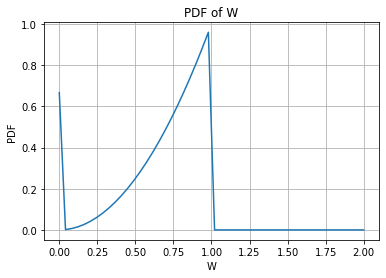
\includegraphics[width=\columnwidth]{solutions/2013/june/70/figures/assignment8pdf.png}
\end{center}
\end{figure}

\begin{figure}[htb!]
\begin{center}
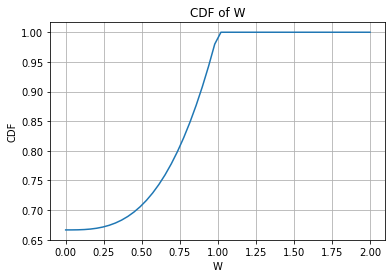
\includegraphics[width=\columnwidth]{solutions/2013/june/70/figures/assignment8cdf.png}
\end{center}
\end{figure}
\end{enumerate}

%
%
\newcommand{\tikzAngleOfLine}{\tikz@AngleOfLine}
  \def\tikz@AngleOfLine(#1)(#2)#3{%
  \pgfmathanglebetweenpoints{%
    \pgfpointanchor{#1}{center}}{%
    \pgfpointanchor{#2}{center}}
  \pgfmathsetmacro{#3}{\pgfmathresult}%
  }

\item A point is chosen at random from a circular disc shown below. What is the probability that the point lies in the sector OAB?\\
\begin{tikzpicture}[
    colorstyle/.style={
       circle, draw=black,fill=black,
       thick, inner sep=0pt, minimum size=2 mm,
       outer sep=0pt
        },
    scale=2]
\draw (0,0) circle (2cm);
\node at (0,0) [colorstyle,label=below:O]{};
\node at (1,1.732) [colorstyle,label=above:A]{};
\node at (1.732,1) [colorstyle,label=above right:B]{};
\draw (0,0) -- (1,1.732);
\draw (0,0) -- (1.732,1);
\coordinate (O) at (0,0);
\coordinate (A) at (1,1.732);
\coordinate (B) at (1.732,1);
\tikzAngleOfLine(O)(B){\AngleStart}
    \tikzAngleOfLine(O)(A){\AngleEnd}
    \draw[red,<->] (O)+(\AngleStart:1cm) arc (\AngleStart:\AngleEnd:1 cm);
    \node[circle,fill=green] at ($(O)+({(\AngleStart+\AngleEnd)/2}:1.5 cm)$) {x};
\end{tikzpicture}\\
( where $\angle$AOB = x radians )
\begin{multicols}{2}
    \begin{enumerate}
        \item $\frac{2x}{\pi}$
        \item $\frac{x}{\pi}$
        \item $\frac{x}{2\pi}$
        \item $\frac{x}{4\pi}$
    \end{enumerate}
\end{multicols}
%
\solution
The joint pdf is given by:
\begin{equation}
 \texorpdfstring{f\textsubscript{r$\theta$}}{f r $\theta$}(r,\theta)= \begin{cases}
                        \dfrac{r}{\pi R^2}  & \text{if 0 $<$ r $<$ R , 0 $<$ $\theta$ $<$ 2$\pi$ }\\
                        0  & \text{otherwise}
                        \end{cases}
\end{equation}
Let A $\equiv$ (R,  $\theta _2$) and B $\equiv$ (R,  $\theta _1$). \\
Hence,
\begin{equation}
(\theta _2 - \theta _1)= x    
\end{equation}
We want $\theta$ $\in$ ($\theta _1$ , $\theta _2$) and r $\in$ (0,R) for point to lie in the sector.
Let the point to be chosen be (r, $\theta$).\\
So, Required probability is:
\begin{align}
 \nonumber  \pr{\theta_1<\theta<\theta_2 , 0<r<R}\\
    =& \Int_{\theta_1}^{\theta_2} \Int_{0}^{R} \dfrac{r}{\pi R^2} \,dr\,d\theta \displaybreak \\
    =& \Int_{\theta_1}^{\theta_2} \dfrac{1}{\pi R^2} \dfrac{r^2}{2} \Bigg|_0^R \\
    =& \Int_{\theta_1}^{\theta_2} \dfrac{R^2}{2\pi R^2} \,d\theta   \\
    =& \Int_{\theta_1}^{\theta_2} \dfrac{1}{2\pi} \,d\theta\\
    =& \dfrac{\theta}{2\pi} \Bigg|_{\theta_1}^{\theta_2} \\
    =& \dfrac{\theta_2 - \theta_1}{2\pi} \\
    =& \dfrac{x}{2\pi}
\end{align}
    
$\therefore$The correct answer is \textbf{option (3)} \Large $\frac{x}{2\pi}$.


\end{enumerate}

\section{Transformation of Variables}
\renewcommand{\theequation}{\theenumi}
\renewcommand{\thefigure}{\theenumi}
\renewcommand{\thetable}{\theenumi}
\begin{enumerate}[label=\thesection.\arabic*.,ref=\thesection.\theenumi]
\numberwithin{equation}{enumi}
\numberwithin{figure}{enumi}
\numberwithin{table}{enumi}

\item Let X be a random variable with pdf
\begin{align}
    f_{X}(x)=\begin{cases} 
            \frac{2x}{\pi^2}  &  0<x<\pi\\
            0 & \text{otherwise}
            \end{cases} 
\end{align}
Let Y = $\sin{X}$, then for $0<y<1$, the pdf of Y is given by,
\begin{enumerate}[label = (\Alph*)]
    \item  $\frac{2\pi}{\sqrt{1-y^2}}$\\
    \item  $\frac{\pi}{2}\sqrt{1-y^2}$\\
    \item  $\frac{2}{\pi}\sqrt{1-y^2}$\\
    \item  $\frac{2}{\pi\sqrt{1-y^2}}$
\end{enumerate}
\solution
From the given information, 
% Given pdf of X as
% \begin{align}
%     f_{X}(x)=\begin{cases} 
%             \frac{2x}{\pi^2}  &  0<x<\pi\\
%             0 & \text{otherwise}
%             \end{cases} 
% \end{align}
\begin{align}
    F_X(x) &= \pr{X\leq x}\\
    &=\begin{cases} 
            0 & x\le 0\\
            \frac{x^2}{\pi^2}  &  0<x<\pi\\
            1 & x\ge \pi
            \end{cases}
            \label{trans/1/a}
\end{align}
after integration.  Consequently, 
\begin{align}
    F_Y(y) &= \pr{Y\leq y}\\
     &= \pr{\sin{X}\leq y}
\end{align}
From Fig. \ref{trans/1/plot}, 
\begin{figure}[!ht]
    \centering
    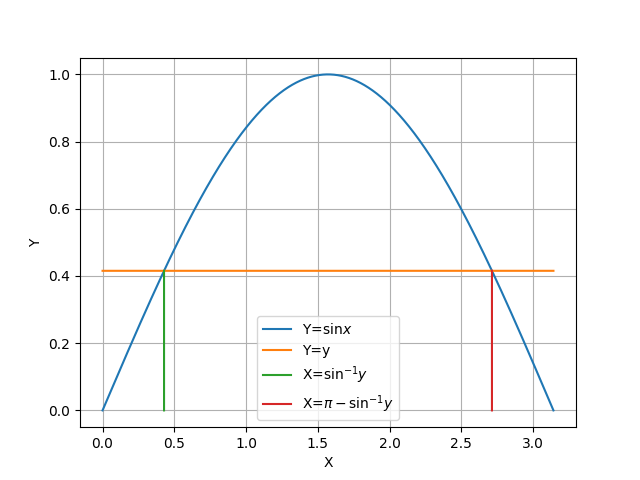
\includegraphics[width=\linewidth]{trans/solutions/1/plot.png}
    \caption{$Y=\sin X$ plot}
    \label{trans/1/plot}
\end{figure}
%
\begin{multline}
    \sin{X}\leq y 
    \\
    \implies \cbrak{X\leq \sin^{-1}{y} \cup X\geq \pi-\sin^{-1}{y}} 
\end{multline}
\begin{align}
    \implies F_Y(y) &= \pr{X\leq \sin^{-1}{y}} \nonumber \\
    & \quad +\pr{X\geq \pi-\sin^{-1}{y}}\\
     &= F_X(\sin^{-1}{y}) \nonumber \\
     & \quad +1-\pr{X\leq \pi-\sin^{-1}{y}}\\
    \implies F_Y(y) &= 1 + F_X(\sin^{-1}{y})-F_X(\pi-\sin^{-1}{y})
    \label{trans/1/b}
\end{align}
Substituting from  \eqref{trans/1/a} in \eqref{trans/1/b}
\begin{align}
 F_Y(y) &= \frac{\brak{\sin^{-1}{y}}^2}{\pi^2}+1-\frac{\brak{\pi-\sin^{-1}{y}}^2}{\pi^2}\\
    &= \frac{2\sin^{-1}{y}}{\pi}
\end{align}
%
\begin{align}
    \therefore     f_Y(y) &= \diff{F_Y(y)}{y}\\
    &= \frac{2}{\pi\sqrt{1-y^2}}
\end{align}
Hence, option(D) is correct.


\end{enumerate}

\section{Independent Random Variables}
\renewcommand{\theequation}{\theenumi}
\renewcommand{\thefigure}{\theenumi}
\renewcommand{\thetable}{\theenumi}
\begin{enumerate}[label=\thesection.\arabic*.,ref=\thesection.\theenumi]
\numberwithin{equation}{enumi}
\numberwithin{figure}{enumi}
\numberwithin{table}{enumi}


\item Let  $X\in \{ 0,1 \}$ and $Y\in \{ 0,1 \}$ be two independent binary random variables. If $\pr{X=0}$ = p and  $\pr{Y=0}$ = q, then $\pr{X+Y \geqslant 1}$) is equal to 
\begin{enumerate}
\item $pq+(1-p)(1-q)$ 
\item  $pq$    
\item $p(1-q)$ 
\item  $1-pq$  
\end{enumerate}
%
\solution
%
%From the given information, 
\begin{align}
    p_{X}(n) &= 
\begin{cases}
p & n=0
\\
1-p & n=1
\end{cases}\label{sum/1/1}
\\
p_{Y}(n) &= 
\begin{cases}
q & n=0
\\
1-q & n=1
\end{cases}\label{sum/1/2}
\end{align}
%
  The characteristic functions of $X$ and $Y$ are 
%
\begin{align}
\phi_X(z)&=\mean{z^{-X}} =  p+(1-p)z^{-1}
\\
\phi_Y(z)&= q+(1-q)z^{-1}
\end{align}
and the CF of $  Z=X+Y$ is 
\begin{align}
\phi_{X+Y}(z)&=\mean{z^{-(X+Y)}} \\
               &=\phi_X(z)\times \phi_Y(z)
               \\
  & =\sbrak{p+(1-p)z^{-1}}\sbrak{q+(1-q)z^{-1}}
  \end{align}
  \begin{multline}
\implies \phi_{Z}(z) = pq+(p+q-2pq)z^{-1}\\
  +(1-p)(1-q)z^{-2}
\end{multline}
yielding 
%   From equation \eqref{sum/1/1}, we get\\
%     The pmf of Z is 
\begin{align}
    p_{Z}(n) = 
\begin{cases}
pq & n=0
\\
p+q-2pq & n=1\\
(1-p)(1-q) & n=2
\end{cases}\label{sum/1/3}
\end{align}
Thus, 
\begin{align}
    \pr{X+Y\geq1} = 1 - \pr{Z<1}= 1-pq   
\end{align}
%
\item Two independent random variables $X$ and $Y$ are uniformly distributed in the interval $\sbrak{-1,1}$. The probability that $\max \brak{X,Y}$ is less than $\dfrac{1}{2}$ is 
\begin{multicols}{4}
\begin{enumerate}
\item $\dfrac{3}{4}$
\item $\dfrac{9}{16}$
\item $\dfrac{1}{4}$
\item $\dfrac{2}{3}$
\end{enumerate}
\end{multicols}
\solution
%
%%
The  CDF of the X is 
 \begin{align}
 F_{X}(x)=\pr{ X<x }= \int _{-1}^{x} f_{X}(x) dx\\
 = \int _{-1}^{x} \dfrac{1}{2} dx= \dfrac{1}{2} \left( x-(-1) \right) = \dfrac{1}{2}( x+1) 
 \intertext{so} F_{X}(x)=\begin{cases}
 0   &   x<-1\\
 \dfrac{1}{2} (x+1) &   -1<x<1\\
 1  &   x>1 
 \end{cases}
  \label{indep/2/eq:9}
 \end{align}
$\because X, Y$ are independent,
 \begin{align}
 \pr{\max \brak{X,Y} < \dfrac{1}{2}}&= \pr{X<\dfrac{1}{2},  Y<\dfrac{1}{2} }
 \\
 & = \pr{ X<\dfrac{1}{2} } \times  \pr{Y<\dfrac{1}{2} }
 \label{indep/2/eq:7}
\\ 
& =\sbrak{F_{X}\left(\dfrac{1}{2} \right)}^2
\\
&= \dfrac{9}{16}
\end{align} 
upon substituting from   \eqref{indep/2/eq:9}.
So option 2 is correct answer 
%
\item Suppose that $X_1,X_2,X_3,...,X_{10}$ are i.i.d, N(0,1). Which of the following statements are correct ?
\begin{enumerate}[label = (\Alph*)]
    \item $\pr{X_1>X_2+X_3+...+X_{10}}=\frac{1}{2}$
    \item $\pr{X_1>X_2X_3...X_{10}}=\frac{1}{2}$
    \item $\pr{\sin{X_1}>\sin{X_2}+\sin{X_3}+...+\sin{X_{10}}}=\frac{1}{2}$
    \item $\pr{\sin{X_1}>\sin({X_2+X_3+\ldots+X_{10}})}=\frac{1}{2}$
\end{enumerate}
\solution
%
\begin{lemma}
    If $X \sim \mathcal{N}(0,1)$ then $Y =-X$ also follows standard normal distribution.
\end{lemma}
\begin{proof}
\begin{align}
    P(Y \leq u) &= P(-X \leq u) \\
    &= P(X > -u) \\
    &= 1 - P(X \leq -u) \\
    &= 1 - (1 - P(X \leq u) \\
    &= P(X \leq u) 
\end{align}
As the distribution is symmetric, 
\begin{align}
 P(X\leq -u)=P(X\geq u)= 1-P(X\leq u)   
\end{align} 
\end{proof}
\begin{lemma}
    If $n$ is an even number and $g(x)$ is an odd function, then,
    \begin{enumerate}
        \item 
    \begin{multline}\label{indep/3/equality}
        \pr{g(X_1)>\sum_{k=2}^ng(X_k)} \\=
        \pr{g(X_1)<\sum_{k=2}^ng(X_k)} \\
        = \frac{1}{2}
    \end{multline}
    \item 
    \begin{multline}
        \pr{g(X_1)>\prod_{k=2}^ng(X_k)}\\=
        \pr{g(X_1)<\prod_{k=2}^ng(X_k)} = \frac{1}{2}
    \end{multline}
    
\end{enumerate}
\end{lemma}
\begin{proof}
\begin{enumerate}
\item 
\begin{multline}
    \pr{g(X_1)>\sum_{k=2}^ng(X_k)}\\=
    \pr{g(-X_1)<\sum_{k=2}^ng(-X_k)}\\=
    \pr{g(X_1)<\sum_{k=2}^ng(X_k)}
\end{multline}
%
As the cases
\begin{align}
    g(X_1)>\sum_{k=2}^ng(X_k)
\end{align}
and
\begin{align}
    {g(X_1)<\sum_{k=2}^ng(X_k)}
\end{align}
are complementary to each other, 
\begin{align}\label{indep/3/sum}
 \pr{g(X_1)>\sum_{k=2}^ng(X_k)}=\frac{1}{2}    
\end{align}
%
\item Similarly, 
\begin{multline}
    \pr{g(X_1)>\prod_{k=2}^ng(X_k)}\\=
    \pr{g(-X_1)<\prod_{k=2}^ng(-X_k)}\\=
    \pr{g(X_1)<\prod_{k=2}^ng(X_k)}
\end{multline}
As they follow the same distribution, the above expression is true. Thus we have
\begin{align}
    %\label{indep/3/equality}
    \pr{g(X_1)>\prod_{k=2}^ng(X_k)}=
    \pr{g(X_1)<\prod_{k=2}^ng(X_k)}
\end{align}
%
As the cases
\begin{align}
    g(X_1)>\prod_{k=2}^ng(X_k)
\end{align}
and
\begin{align}
    {g(X_1)<\prod_{k=2}^ng(X_k)}
\end{align}
are complementary to each other and from 
 \eqref{indep/3/equality} we have
\begin{align}\label{indep/3/prod}
 \pr{g(X_1)>\prod_{k=2}^ng(X_k)}=\frac{1}{2}    
\end{align}
\end{enumerate}
\begin{enumerate}[label = (\Alph*)]
    \item 
    From \eqref{indep/3/sum} , taking $g(x)=x$,
    \begin{align}
        \pr{X_1>X_2+...+X_{10}}=\frac{1}{2}
    \end{align}
\item
From \eqref{indep/3/prod} taking $g(x)=x$
        \begin{align}
         \pr{X_1>X_2X_3...X_{10}}=\frac{1}{2}   
        \end{align}
\item 
From \eqref{indep/3/sum} taking $g(x)=\sin{x}$
        \begin{align}
         \pr{\sin{X_1}>\sin{X_2}+...+\sin{X_{10}}}=\frac{1}{2}   
        \end{align}
\item \begin{multline}
        \pr{\sin{X_1}>\sin{(X_2+...+X_{10})}}\\=\pr{\sin{(-X_1)}<\sin{(-X_2-...-X_{10})}}\\
        =\pr{\sin{X_1}<\sin{(X_2+...+X_{10})}}
    \end{multline}
    As they follow the same distribution, the above expression is true.
    Thus we have
    \begin{multline} 
    \pr{\sin{X_1}>\sin{(X_2+...+X_{10}})}\\
        =\pr{\sin{X_1}<\sin{(X_2+...+X_{10}})}    
    \end{multline}
    Also, as $X_1$ is a continuous random variable
    \begin{align}
       \pr{\sin{X_1}=\sin{(X_2+...+X_{10})}}=0
    \end{align}
     As the cases
     \begin{align}
      {X_1>X_2+...+X_{10}}   
     \end{align}and 
     \begin{align}
         {X_1<X_2+...+X_{10}}
     \end{align}are complementary to each other 
        \begin{align}
         \pr{\sin{X_1}>\sin{(X_2+...+X_{10}})}=\frac{1}{2}   
        \end{align}
\end{enumerate}
\end{proof}

\item Which of the following conditions imply independence of the random variables $X$
and $Y$ ?
\begin{enumerate}
    \item  $\pr{X\ \mathop{>}\ a|Y\ \mathop{>}\ a} = \pr{X\ \mathop{>}\ a}\ \forall\ a\ \in\ \mathbb{R}$\\ 
    \item  $\pr{X\ \mathop{>}\ a|Y\ \mathop{<}\ b} = \pr{X\ \mathop{>}\ a}\ \forall\ a,\ b\ \in\ \mathbb{R}$\\ 
    \item  $X$ and $Y$ are uncorrelated.\\
    \item  $E[(X-a)(Y-b)] = E(X-a)\ E(Y-b)\ \forall\ a,\ b \in\ \mathbb{R}$\\
\end{enumerate}
%
\solution
%

\begin{definition}
    Two random variables $X$ and $Y$ are independent when the joint probability distribution of random variables is product of their individual probability distributions i.e for all sets A,B
    \begin{align}
        \label{indep/4/eq1} \pr{X\in A,Y \in B}=\pr{X \in A}\pr{Y \in B}
    \end{align}
    Alternatively, 
    \begin{align}
        \label{indep/4/eq1/cdf} F_{X,Y}\brak{a,b}=F_X\brak{a}F_Y\brak{b}
     \end{align}
  
\end{definition}
\begin{lemma}
From \eqref{indep/4/eq1/cdf}, it follows that 
\begin{align}
    \implies f_{X,Y}\brak{a,b}=f_X\brak{a}f_Y\brak{b}
    \label{indep/4/eq1/pdf}
\end{align}
\end{lemma}
\begin{proof}
    From \eqref{indep/4/eq1/cdf},
    \begin{align}
        \frac{\partial^2 F_{X,Y}\brak{a,b}}{\partial b \partial a}=\frac{\partial F_X\brak{a} }{\partial a}\frac{\partial F_Y\brak{b} }{\partial b} 
    \end{align}
    yielding     \eqref{indep/4/eq1/pdf}.
\end{proof}


\begin{enumerate}
     \item  From the given information, 
     \begin{align}
        \pr{X>a,Y>a} &=         \pr{X>a}\pr{Y>a}
        \\
        &= \sbrak{1-F_X\brak{a}}\sbrak{1-F_Y\brak{a}}
        \label{indep/4/eq1/sp/1}
     \end{align}
    \begin{multline}
\because \pr{X>a}-\pr{Y<a}\\=\pr{X>a,Y>a}+\pr{X>a,Y<a}\\-\pr{X>a,Y<a}-\pr{X<a,Y<a}, 
\\
\pr{X>a,Y>a} =         1-F_X\brak{a}-F_Y\brak{a}\\ +F_{X,Y}\brak{a,a}
    \end{multline}
which, upon substituting from         \eqref{indep/4/eq1/sp/1} yields
\begin{align}
\implies F_{X,Y}\brak{a,a}=F_X\brak{a}F_Y\brak{a}
\label{indep/4/eq1/sp}
\end{align}
which is a special case of \eqref{indep/4/eq1} for $b=a$.  The spectrum of conditions for independence is hence underrepresented. 
Thus, the given  condition does not imply independence of $X$ and $Y$.    
% \begin{example}
%     Consider two random variables $X$,$Y \in \{0,1,2\}$ with the probabilities of the ordered pairs \brak{X,Y} given in the Table\ref{indep/4/table1}.  The given
%     distribution satisfies 
% \end{example}
%     \begin{table}[!ht]
%      \centering
%      \resizebox{\columnwidth}{!}{
% \begin{tabular}{|l|c|c|c|}
%     \hline
%     \diagbox{$X$}{$Y$}&0&1&2\\ 
%     \hline
%      0&0.2&0.1 &0.1\\     \hline
%      1&0.2&0.1&0.05\\     \hline
%      2&0.1&0.1&0.05\\     \hline
%     \hline
%     \end{tabular}}
%     \caption{\pr{X,Y}}
%     \label{indep/4/table1}
%         \end{table}    
    
%     Case 1: $a<0$
%     \begin{align}
%         \pr{X>a|Y>a}=1=\pr{X>a}
%     \end{align}
%     Case 2: $0\leq a <1$
%     \begin{align}
%         \pr{X>a|Y>a}=\frac{\pr{X,Y>a}}{\pr{Y>a}}=\frac{0.3}{0.5}=0.6\\
%         \pr{X>a}=\pr{X=1}+\pr{X=2}=0.6
%     \end{align}
%     Case 3: $1\leq a <2$
%     \begin{align}
%         \pr{X>a|Y>a}=\frac{\pr{X,Y>a}}{\pr{Y>a}}=\frac{0.05}{0.2}=0.25\\
%         \pr{X>a}=\pr{X=2}=0.25
%     \end{align}
%     Case 4: $a\geq 2$
%     \begin{align}
%         \pr{X>a|Y>a}=\frac{\pr{X,Y>a}}{\pr{Y>a}}
%     \end{align}
%     is not defined as $\pr{Y>a}=0$.
%     In all the cases, $\pr{X>a|Y>a}=\pr{X>a}$ is true.
    
%     Consider,
%     \begin{align}
%         \pr{X=1,Y=2}=0.05
%     \end{align}
%     \begin{multline}
%         \pr{X=1}\pr{Y=2}=0.35\times0.2=0.7\\\neq\pr{X=1,Y=2}
%     \end{multline} 
%     Clearly, $X$ and $Y$ are not independent. 
    
     {\em Option 1 is incorrect}.
    
    \item From Bayes theorem,
    \begin{align}
        \pr{X>a|Y<b}&=\pr{X>a}
    \end{align}
    \begin{multline}
            \label{indep/4/eq3}
            \implies \pr{X>a,Y<b} \\ =\pr{X>a}\pr{Y<b}
        \end{multline}
    for all $a,b\in R$. 
    \begin{multline}
    \because     F_Y\brak{b}=\pr{X>a,Y<b} \\ +\pr{X<a,Y<b}, 
    \end{multline}
    \begin{multline}
    \pr{X>a,Y<b} \\= F_Y\brak{b}-F_{X,Y}\brak{a,b}
    \\
    \implies           F_Y\brak{b}-F_{X,Y}\brak{a,b} \\=\brak{1-F_X\brak{a}}F_Y\brak{b}\\
    \text{or, }
        F_{X,Y}\brak{a,b}=F_X\brak{a}F_Y\brak{b}
    \end{multline}
    upon substituting from  \eqref{indep/4/eq3} and simplifying.
     Thus, $X$ and $Y$ are independent. 
    
{\em Option 2 is correct}.
\item  We prove through a counterexample.
\begin{definition}
    Two random variables $X$ and $Y$ are uncorrelated if their covariance is zero, i.e., 
    \begin{align}
        \cov{X}{Y}=\mean{XY}-\mean{X}\mean{Y}=0
    \end{align}
\end{definition}
    % Uncorrelatedness does not imply independence.
    Let $X\sim U \sbrak{-1,1}$ be a uniformly distributed random variable such that 
    \begin{align}
        f_X\brak{x}=
        \begin{cases}
        \frac{1}{2} & -1\leq x \leq 1\\
        0 & otherwise
        \end{cases}\\
        \mean{X}=\int_{-1}^{1}x f\brak{x} dx=0
    \end{align}
    Let 
    \begin{align}
        Y=X^2.
    \end{align}
   so that  $X$ and $Y$ are dependent.  Then, 
    \begin{align}
        \cov{X}{Y}&=\mean{XY}-\mean{X}\mean{Y}\\
        &=\mean{X^3}-0\times \mean{Y}\\
        &=\int_{-1}^{1}x^3 f\brak{x} dx=0
    \end{align}
    $X$ and $Y$ are uncorrelated but not independent.
    
    {\em Option 3 is incorrect}
    
    \item Given that,
    \begin{align}
        \mean{\brak{X-a}\brak{Y-b}}=\mean{X-a}\mean{Y-b}
    \end{align}
    \begin{multline}
    \implies     \cov{X-a}{Y-b}=
    \\
        \mean{\brak{X-a}\brak{Y-b}}\\-\mean{X-a}\mean{Y-b}
    \end{multline}
    \begin{align}
        \text{or, } \cov{X-a}{Y-b}=0=\cov{X}{Y}
    \end{align}
    From option 3, it follows that $X$ and $Y$ are not necessarily independent.
    
    \textbf{Option 4 is incorrect.}
\end{enumerate}

%
\item Let X and Y be two independent and identically distributed (I.I.D) random variables uniformly distributed in (0,1). Let $Z = max(X,Y)$ and $W = min(X,Y)$ , then the probability that $[Z-W >\frac{1}{2}]$ is\\
\\(A) $\frac{1}{2}$\\
\\(B) $\frac{3}{4}$\\
\\(C) $\frac{1}{4}$\\
\\(D) $\frac{2}{3}$    
%
\solution

X and Y are two independent random variables. \\
Let
\begin{align}
    f_X\brak{x} &= \Pr\brak{X=x} \\
    f_Y\brak{y} &= \Pr\brak{Y=y}  \\
    f_V\brak{v} &= \Pr\brak{V=v}
\end{align}
be the probability densities of random variables X ,Y and V=X-Y.\\
The density for X is \\
\begin{align}
\label{june2018-50eq:_pdf_x}
f_{X}(x)  = 
\begin{cases}
1 & 0 \le x \le 1
\\
0 & otherwise
\end{cases}
\end{align}
We have ,
\begin{equation}
    V= X-Y \iff v= x- y \iff x = v+y
\end{equation}
The density of X can also be represented as,
\begin{align}
\label{june2018-50eq:pdf_x}
f_{X}(v+y)  = 
\begin{cases}
1 & 0 \le v+y \le 1
\\
0 & otherwise
\end{cases}
\end{align}
and the density of Y is,
\begin{align}
\label{june2018-50eq:pdf_y}
f_{Y}(y)  = 
\begin{cases}
1 & 0 \le y \le 1
\\
0 & otherwise
\end{cases}
\end{align}
The density of V i.e. $V=X-Y $ is given by the convolution of $f_X(-v)$ with $f_Y(v)$.
\begin{equation}
    f_V(v) =  \int_{- \infty}^{\infty} f_X(v+y)f_Y(y) \,dy 
\end{equation}
From \ref{june2018-50eq:pdf_x} and \ref{june2018-50eq:pdf_y} we have, \\
The integrand is 1 when,
\begin{align}
    0 \le y \le 1 \\
    0 \le v+y \le 1 \\
    -v \le y \le 1-v
\end{align}
and zero, otherwise. \\
Now when $-1 \le v \le 0$ we have, 
\begin{align}
    f_V(v) &=   \int_{-v}^{1} \,dy  \\
          &= (1 - (-v)) \\
          &= 1+v
\end{align}

For $0 \le v \le 1$ we have, 
\begin{align}
    f_V(v) &=   \int_{0}^{1-v} \,dy  \\
          &= (1-v - (0)) \\
          &= 1-v
\end{align}

Therefore the density of V is given by
\begin{align}
\label{june2018-50eq:pdf_v}
f_{V}(v)  = 
\begin{cases}
1+v & -1 \le v \le 0
\\
1-v & 0 < v \le 1
\\
0 & otherwise
\end{cases}
\end{align}

The plot for PDF of $V $ can be observed at figure \ref{june2018-50fig:The PDF of V}
\begin{figure}[!ht]
       \centering
    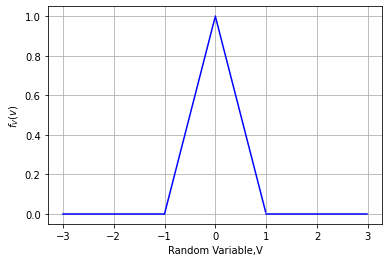
\includegraphics[width=\columnwidth] {solutions/2018/june/50/Assignment_3_Fig_1.png}
    \caption{The PDF of V}
    \label{june2018-50fig:The PDF of V}
\end{figure}

The CDF of V is defined as,
\begin{equation}
    F_V(v) = \Pr\brak{V \le v}
\end{equation}
Now for $ v \le 0 $,
 \begin{align}
    \Pr\brak{V\le v} &=  \int_{-\infty}^{v}f_{V}(v) \,dv  \\
          &=  \int_{-1}^{v} (1+v) \,dv  \\
          &=  \left(\dfrac{v^2}{2}+v \right) \Biggr|_{-1}^{v}  \\
          &=   \left(\left(\dfrac{v^2}{2}+v \right) - \left(\dfrac{1}{2} -1 \right)\right) \\
          &= \dfrac{v^2+2v +1}{2}
\end{align}
Similarly for $v \le 1$,
\begin{align}
    \Pr\brak{V\le v} &=  \int_{-\infty}^{v}f_{V}(v) \,dv  \\
          &=  \dfrac{1}{2} + \int_{0}^{v}(1-v)\,dz  \\
          &=  \dfrac{-v^2+2v+1}{2}
\end{align}

The CDF is as below: 
\begin{align}
\label{june2018-50eq:cdf_v}
F_{V}(v)  = 
\begin{cases}
0 & v < -1
\\
\dfrac{v^2+2v + 1}{2} &  v \le 0
\\
\dfrac{-v^2+2v+1}{2} &  v \le 1
\\
1 & v > 1
\end{cases}
\end{align}

The plot for CDF of $V $ can be observed at figure \ref{june2018-50fig:The CDF of V}\\

\begin{figure}[!ht]
       \centering
    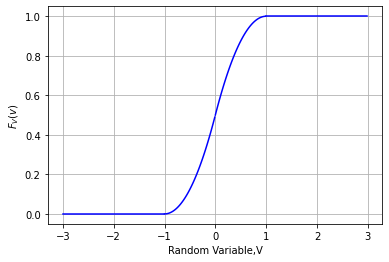
\includegraphics[width=\columnwidth] {solutions/2018/june/50/Assignment_3_Fig_2.png}
    \caption{The CDF of V}
    \label{june2018-50fig:The CDF of V}
\end{figure}

We need  $\pr{Z-W >\frac{1}{2}}$ where $Z = max(X,Y)$ and $W = min(X,Y)$. Now,

\begin{align}
\label{june2018-50eq:pdf_v}
Z-W  = 
\begin{cases}
X-Y & \text{for } X \geq Y
\\
Y-X & \text{for } X < Y
\end{cases}
\end{align}

Therefore,
\begin{align}
    \pr{Z-W >\frac{1}{2}} &= \pr{X-Y>\frac{1}{2},X \geq Y} \nonumber \\
    &+\pr{Y-X > \frac{1}{2}, X < Y}\\
    &= \pr{X-Y>\frac{1}{2}} +\pr{Y-X>\frac{1}{2}}\\
    &= \pr{V > \frac{1}{2}} + \pr{-V > \frac{1}{2}}\\
    &= 1 - \pr{V \leq \frac{1}{2}} + \pr{V < \frac{-1}{2}}\\
    &= 1-F_V(\frac{1}{2}) + F_V(-\frac{1}{2})\\
    &= 1 -\frac{7}{8} + \frac{1}{8}\\
    &= \frac{1}{4}
\end{align}

Hence the correct answer is option (C).


%
%
\item Let $X$ and $Y$ be independent exponential random variables. If $E[X]=1$ and $E[Y]=\frac{1}{2}$ then $\pr{X>2Y|X>Y}$ is
\begin{multicols}{2}
    \begin{enumerate}[label=\arabic*.]
        \item \Large$\frac{1}{2}$ \\
        \item $\frac{1}{3}$
        \item $\frac{2}{3}$ \\
        \item $\frac{3}{4}$
    \end{enumerate}
\end{multicols}
%
\solution
Since $X$ and $Y$ are exponential random variables with means'
\begin{align}
    E[X] = 1 \text{ and } E[Y] = \frac{1}{2}
\end{align}
Marginal PDFs of $X$ and $Y$  are given by
\begin{align}
    f_X(x)= e^{-x} , x>0 \\
    f_Y(y) = 2e^{-2y} , y>0
\end{align}
CDFs for $X$ and $Y$ are
\begin{align}
    F_X(b) &= \int_0^b f_X(x)\,d_x\\
           &= \int_0^b  e^{-x}\,d_x\\
           &= 1-e^{-b}
\end{align}
\begin{align}
    F_Y(b) &= \int_0^b f_Y(y)\,d_y\\
           &= \int_0^b 2e^{-2y}\,d_y\\
           &= \left[-e^{-2y}\right]_0^b\\
           &= 1-e^{-2b}
\end{align}
Now,
\begin{align}
    \pr{X>2Y|X>Y} &= \dfrac{\pr{X>2Y\,,\,X>Y} }{\pr{X>Y}}\\
                  &= \dfrac{\pr{X>2Y}}{\pr{X>Y}} \label{dec2017-59:simul1}
\end{align}
\begin{align}
    \pr{X>Y} &= \pr{Y<X}\\
             &= E[F_Y(X)]\\
             &= \int_0^\infty F_Y(X)\,f_X(x)\,d_x\\
             &= \int_0^\infty (1-e^{-2x})\,e^{-x}d_x\\
             &= \left[\frac{e^{-x}}{-1} - \frac{e^{-3x}}{-3}\right]_0^\infty\\
            &=(0+1)+\frac{1}{3}(0-1) \\
             &= \frac{2}{3} \label{dec2017-59:simul2}
\end{align}
\begin{align}
    \pr{X>2Y} &= \pr{Y<\frac{X}{2}}\\
              &= E[F_Y(X/2)]\\
              &=  \int_0^\infty F_Y(X/2)\,f_X(x)\,d_x\\
              &= \int_{0}^{\infty}(1-e^{-x})\,e^{-x}d_x\\
              &= \left[\frac{e^{-x}}{-1} - \frac{e^{-2x}}{-2}\right]_0^\infty\\
              &= (0+1) + \frac{1}{2}(0-1)\\
              &= \frac{1}{2} \label{dec2017-59:simul3}
\end{align}
Putting \eqref{dec2017-59:simul2} and \eqref{dec2017-59:simul3} in \eqref{dec2017-59:simul1}
\begin{align}
    \pr{X>2Y\,|\,X>Y} &= \frac{1/2}{2/3}\\
                  &= \frac{3}{4}
\end{align}
$\therefore$ Option 4 is the correct answer.
%
%
\item A fair die is thrown two times independently. Let $X,Y$ be the outcomes of these two throws and $Z=X+Y$. Let $U$ be the remainder obtained when $Z$ is divided by 6. Then which of the following statement(s) is/are true?
\begin{enumerate}
    \item $X$ and $Z$ are independent \label{dec2016-103:option 1}
    \item $X$ and $U$ are independent \label{dec2016-103:option 2}
    \item $Z$ and $U$ are independent \label{dec2016-103:option 3}
    \item $Y$ and $Z$ are not independent \label{dec2016-103:option 4}
\end{enumerate}
%
\solution
Let $X \in \{1,2,3,4,5,6\}$ represent the random variable which represents the outcome of the first throw of a dice. Similarly, $Y \in \{1,2,3,4,5,6\}$ represents the random variable which represents the outcome of the second throw of a dice.
\begin{align}
    n(X=i) = 1, \quad i \in \{1, 2, 3, 4, 5, 6\}
\end{align}
\begin{align}
    \Pr(X=i) = 
	\begin{cases}
	\frac{1}{6}   &  i \in \{1, 2, 3, 4, 5, 6\}\\ ~\\[-1em]
	0 & \text{otherwise}
	\end{cases}
\end{align}
Similarly, 
\begin{align}
    \Pr(Y=i) = 
	\begin{cases}
	\frac{1}{6}   &  i \in \{1, 2, 3, 4, 5, 6\}\\ ~\\[-1em]
	0 & \text{otherwise}
	\end{cases}
\end{align}
\begin{align}
    Z &= X+Y
    \\ \text{Let } z &\in \{1, 2, \hdots, 11, 12\}
    \\\Pr{(Z=z)} &= \Pr{(X+Y = z)}
    \\ &= \sum_{x=0}^z \Pr{(X=x)}\Pr{(Y=z-x)}
    \\ &= (6 - \abs{z-7}) \times\frac{1}{6}\times\frac{1}{6}
    \\ &= \frac{6 - \abs{z-7}}{36}
    \\\Pr(Z=z) &= 
	\begin{cases}
	\frac{6 - \abs{z-7}}{36}   &  z \in \{1, 2, \hdots, 11, 12\}\\ ~\\[-1em]
	0 & \text{otherwise}
	\end{cases}
\end{align}
$U$ is the remainder obtained when $Z$ is divided by 6.
\begin{align}
    \text{Let } u &\in \{0, 1, 2, 3, 4, 5\}
    \\\Pr{(U=u)} &= \sum_{k=0}^2\Pr{(Z = 6k+u)}
    \\\Pr{(U=0)} &= \Pr{(Z = 0)} + \Pr{(Z = 6)} + \Pr{(Z = 12)}
    \\ &= 0 + \frac{5}{36} + \frac{1}{36} = \frac{1}{6}
    \\ \text{for } u &\in \{1, 2, 3, 4, 5\}
    \\\Pr{(U=u)} &= \Pr{(Z = 0+u)} + \Pr{(Z = 6+u)}
    \\&= \frac{6 - \abs{u-7}}{36} +  \frac{6 - \abs{6+u-7}}{36}
    \\&= \frac{6 - (7-u)}{36} +  \frac{6 - (u-1)}{36}
    \\&= \frac{u - 1 + 7 - u}{36} = \frac{6}{36}
    \\&=\frac{1}{6}
    \\\Pr(U=u) &= 
	\begin{cases}
    \frac{1}{6}   &  u \in \{0, 1, 2, 3, 4, 5\}\\ ~\\[-1em]
	0 & \text{otherwise}
	\end{cases}
\end{align}
Now, for checking each option,
\begin{enumerate}
    
\item Checking if $X$ and $Z$ are independent
\begin{align}
    p_1 &= \Pr{(Z=z, X=x)}
    \\ &= \Pr{(Y=z-x, X=x)}
    \\ &= \Pr{(Y=z-x)} \times \Pr{(X=x)}
    \\ &= \begin{cases}
        \frac{1}{36} & z-x \in \{1, 2, 3, 4, 5, 6\}\\ ~\\[-1em]
        0 & \text{otherwise}
    \end{cases}
\end{align}
\begin{align}
    \Pr{(Z=z)}\times \Pr{(X=x)} &= \frac{6 - \abs{z-7}}{36} \times \frac{1}{6}
    \\&= \frac{6 - \abs{z-7}}{216}
    \\\Pr{(Z=z)}\Pr{(X=x)} &\neq \Pr{(Z=z, X=x)}  \label{dec2016-103:equation 1}
\end{align}
$X$ and $Z$ are not independent from \eqref{dec2016-103:equation 1} and hence option \eqref{dec2016-103:option 1} is false.
\item Checking if $X$ and $U$ are independent
\begin{align}
    p_2 = \Pr{(U=u, X=x)}
\end{align}
\begin{multline}
    p_2 = \Pr{((Z=u) + (Z=6+u)}
    \\+ (Z=12+u), X=x)
\end{multline}
\begin{multline}
    p_2 = \Pr{((Y=u-x) + (Y=6+u-x)}
    \\+ (Y=12+u-x), X=x)
\end{multline}
\begin{align}
    p_2 &= \frac{1}{6} \times \frac{1}{6}
    \\&= \frac{1}{36}
\end{align}
\begin{align}
    \Pr{(U=u)}\times \Pr{(X=x)} &= \frac{1}{6} \times \frac{1}{6}
    \\&= \frac{1}{36}
    \\\Pr{(U=u)}\Pr{(X=x)} &= \Pr{(U=u, X=x)}  \label{dec2016-103:equation 2}
\end{align}
$X$ and $U$ are independent from \eqref{dec2016-103:equation 2} and hence option \eqref{dec2016-103:option 2} is true.
\item Checking if $Z$ and $U$ are independent
\begin{align}
    p_3 &= \Pr{(Z=z| U=u)}
    \\p_3 &= 
    \begin{cases}
        1 & u=1 \text{ and } z=7\\ ~\\[-1em]
        \frac{1}{2} & u=0 \text{ and } z\in\{6,12\}\\ ~\\[-1em]
        \frac{1}{2} & u\in\{2,3,4,5\}  \text{ and } \\&z=u \text{ or } z=6+u\\ ~\\[-1em]
        0 & \text{otherwise}
    \end{cases}
    \\\Pr{(Z=z)} &= \frac{6 - \abs{z-7}}{36}
\end{align}
If $Z$ and $U$ are independent, then
\begin{align}
    \Pr{(Z=z| U=u)} &= \frac{\Pr{(Z=z, U=u)}}{\Pr{(U=u)}}
    \\&= \frac{\Pr{(Z=z)}\Pr{(U=u)}}{\Pr{(U=u)}}
    \\&= \Pr{(Z=z)}
\end{align}
But,
\begin{align}
    \Pr{(Z=z| U=u)} \neq \Pr{(Z=z)} \label{dec2016-103:equation 3}
\end{align}
$X$ and $U$ are not independent from \eqref{dec2016-103:equation 3} and hence option \eqref{dec2016-103:option 3} is false.
\item Checking if $Y$ and $Z$ are independent
\begin{align}
    p_1 &= \Pr{(Z=z, Y=y)}
    \\ &= \Pr{(X=z-y, Y=y)}
    \\ &= \Pr{(X=z-y)} \times \Pr{(Y=y)}
    \\ &= \begin{cases}
        \frac{1}{36} & z-y \in \{1, 2, 3, 4, 5, 6\}\\ ~\\[-1em]
        0 & \text{otherwise}
    \end{cases}
\end{align}
\begin{align}
    \Pr{(Z=z)}\times \Pr{(Y=y)} &= \frac{6 - \abs{z-7}}{36} \times \frac{1}{6}
    \\&= \frac{6 - \abs{z-7}}{216}
    \\\Pr{(Z=z)}\Pr{(Y=y)} &\neq \Pr{(Z=z, Y=y)}  \label{dec2016-103:equation 4}
\end{align}
$X$ and $Z$ are not independent from \eqref{dec2016-103:equation 4} and hence option \eqref{dec2016-103:option 4} is true.
\end{enumerate}
Thus, options \eqref{dec2016-103:option 2} and \eqref{dec2016-103:option 4} are true.
%
\item Suppose $X_1$,$X_2$,$X_3$ and $X_4$ are independent and identically distributed random variables, having density function f. Then,
\begin{enumerate}
\item \pr{X_4 > Max(X_1,X_2) > X_3} = $\frac{1}{6}$
\item \pr{X_4 > Max(X_1,X_2) > X_3} = $\frac{1}{8}$
\item \pr{X_4 > X_3 > Max(X_1,X_2)} = $\frac{1}{12}$
\item \pr{X_4 > X_3 > Max(X_1,X_2)} = $\frac{1}{6}$
\end{enumerate}
%
\solution
The probability density function (pdf) f(x) of a random variable X is defined as the derivative of the cdf F(x): \\
\begin{center}
\begin{math}
    f(x) = \dfrac{d}{d x}F(x).
\end{math}
\end{center} 
It is sometimes useful to consider the cdf F(x) in terms of the pdf f(x):
\begin{center}
    \begin{math}
    F(x) = \int\limits_{-\infty}^x f(t) d t
    \end{math}
\end{center}
The PDF of X is,
\begin{align}
    F_X(x) &= \int\limits_{-\infty}^\infty f(x) d x 
\end{align}
\begin{enumerate}
    \item \pr{X_2 > X_1}
\begin{align}
&= \int\limits_{-\infty}^\infty f_X(x) \int\limits_{-\infty}^x                    f_X(t)\ d t d x \\
&= \int\limits_{-\infty}^\infty f_X(x) F_X(x) d x \\
&= \cfrac{F^{2}_X(x)}{2} \biggr \vert_{-\infty}^{\infty} \\
&= \dfrac{1}{2}.
\end{align}
    \item \pr{X_4>Max(X_1,X_2)>X_3} 
\begin{align}
&= \nonumber \int\limits_{-\infty}^\infty f_X(x) \int\limits_{-\infty}^x f_X(t).\comb{2}{1}. \\ 
&  \sbrak{\int\limits_{-\infty}^t f_X(w) d w} 
   \int\limits_{-\infty}^t f_X(z) d z d t d x \\  
&= \int\limits_{-\infty}^\infty f_X(x) \int\limits_{-\infty}^x 2f_X(t)F^{2}_X(t) d t d x\\
&= \int\limits_{-\infty}^\infty f_X(x). \dfrac{2}{3} F^{3}_X(x) d x \\
&= \dfrac{2}{3}\cfrac{F^{4}_X(x)}{4} \biggr \vert_{-\infty}^{\infty} \\    
&= \dfrac{1}{6}.   
\end{align}
    \item \pr{X_4 > X_3 > Max(X_1,X_2} 
\begin{align}
&= \nonumber \int\limits_{-\infty}^\infty f_X(x) \int\limits_{-\infty}^x f_X(t) 
\int\limits_{-\infty}^t f_X(z). \comb{2}{1}. \\
&  \sbrak{\int\limits_{-\infty}^t f_X(w) d w}\ d z d t d x \\
&= \int\limits_{-\infty}^\infty f_X(x) \int\limits_{-\infty}^x f_X(t) \int\limits_{-\infty}^t 2f_X(z)F_X(t)\ d z d t d x \\
&= \int\limits_{-\infty}^\infty f_X(x) \int\limits_{-\infty}^x f_X(t)F^{2}_X(t) d t d x \\
&= \int\limits_{-\infty}^\infty f_X(x).\dfrac{1}{3}F^{3}_X(x) d x \\
&= \dfrac{1}{3}\cfrac{F^{4}_X(x)}{4} \biggr \vert_{-\infty}^{\infty} \\
&= \dfrac{1}{12}.   
\end{align}
\end{enumerate}
\begin{center}
  $\therefore$ \boxed{\text{\textbf{Option 1,3} are \textbf{correct} answers.}}
\end{center}
%
%
\item Consider a parallel system with two components. The lifetimes of the two components are independent and identically distributed random variables each following an exponential distribution with mean 1. The expected lifetime of the system is:
\begin{enumerate}[label=\Alph*)]
    \item $1$\\[0.5pt]
    \item $\dfrac{1}{2}$\\
    \item $\dfrac{3}{2}$\\
    \item $2$
\end{enumerate}
%
\solution

Consider two random variables X and Y which represent the lifetime of the two components namely A and B.
\begin{equation}
    X \sim Exp(\lambda_X)
\end{equation}
\begin{equation}
    Y \sim Exp(\lambda_Y)
\end{equation}
% \begin{figure}[h]
%     \centering
%     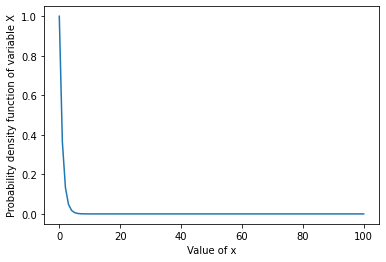
\includegraphics[width=\columnwidth]{solutions/2013/june/42/figures/figure2.png}
%     \caption{P.D.F. of X }
%     \label{june2013-42:june2013-42:fig:fig_label}
% \end{figure}
Let $f_X(x)$ denote the probability distribution function for random variable X.
\begin{align}
f_{X}(x)=
 \begin{cases} 
      \lambda_X  e^{-\lambda_X  x} & x \geq 0 \\
      0 & otherwise
 \end{cases}
\end{align}
Let $f_Y(y)$ denote the probability distribution function for random variable Y.
\begin{align}
f_{Y}(y)=
 \begin{cases} 
      \lambda_Y  e^{-\lambda_Y  y} & y \geq 0 \\
      0 & otherwise
 \end{cases}
 \end{align}
 Let $F_X(x)$ denote the cumulative distribution function for random variable X.
\begin{align}
F_{X}(x)=
 \begin{cases} 
      1-e^{-\lambda_X  x} & x \geq 0 \\
      0 & otherwise
 \end{cases}
\end{align}
Let $F_Y(y)$ denote the cumulative distribution function for random variable Y.
\begin{align}
F_{Y}(y)=
 \begin{cases} 
      1-e^{-\lambda_Y  y} & y \geq 0 \\
      0 & otherwise
 \end{cases}
 \end{align}
\begin{equation}\label{june2013-42:meanx}
    E(X)=\dfrac{1}{\lambda_X}
\end{equation}
\begin{equation}\label{june2013-42:meany}
    E(Y)=\dfrac{1}{\lambda_Y}
\end{equation}
From \ref{june2013-42:meanx} and \ref{june2013-42:meany},
\begin{equation}\label{june2013-42:lambda}
    \lambda_X = \lambda_Y = 1
\end{equation}
\begin{figure}[h]
    \centering
    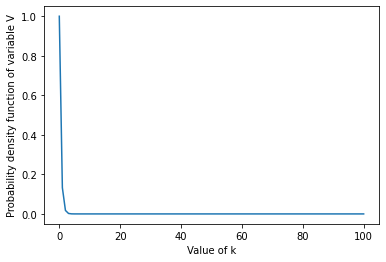
\includegraphics[width=\columnwidth]{solutions/2013/june/42/figures/figure.png}
    \caption{Parallel system}
    \label{june2013-42:fig:fig_label}
\end{figure}
Let Z be a random variable such that $Z=max(X,Y)$
\begin{align}
    P(Z\leq z) &= P(max(X,Y) \leq z)
    \\
    &=P(X\leq z,Y\leq z)
    \\
    &=P(X\leq z) P(Y\leq z)
    \\
    &=(F_X(z)-F_X(0)) (F_Y(z)-F_Y(0))
    \\
    &=1-e^{-(\lambda_X) z}-e^{-(\lambda_Y) z}+e^{-(\lambda_X+\lambda_Y) z}
\end{align}
$P(Z\leq z)$ denotes the probability that the system dies in the first $z$ seconds.\\
\begin{align}
    Expectation &= \int_{0}^{\infty}z \,d(P(Z\leq z))
    \\
\nonumber    &=\int_{0}^{\infty}z(\lambda_Xe^{-(\lambda_X) z}+\lambda_Ye^{-(\lambda_Y) z}\\
&-(\lambda_X+\lambda_Y)e^{-(\lambda_X+\lambda_Y) z}) \,dz
    \\
    &= \dfrac{1}{\lambda_X}+\dfrac{1}{\lambda_Y}-\dfrac{1}{\lambda_X+\lambda_Y}
\end{align}
From \ref{june2013-42:lambda}, 
\begin{equation}
    Expectation=\dfrac{3}{2}
\end{equation}
Therefore, option C correct.


\end{enumerate}
\section{Binomial  Distribution}
\renewcommand{\theequation}{\theenumi}
\renewcommand{\thefigure}{\theenumi}
\renewcommand{\thetable}{\theenumi}
\begin{enumerate}[label=\thesection.\arabic*.,ref=\thesection.\theenumi]
\numberwithin{equation}{enumi}
\numberwithin{figure}{enumi}
\numberwithin{table}{enumi}

\item The probability that a part manufactured by a company will be defective is 0.05. If 15 such parts are selected randomly and inspected,the probability that atleast two parts will be defective is \dots
%
\\
\solution
%
The desired probabilty is 
\begin{align}
    \pr{X \ge 2 } &= 1 - \pr{X < 2 }
    \\
    &= 1-\pr{X=0}-\pr{X=1}
    \\
    &= 1-\comb{15}{0} p^{0} q^{15} -\comb{15}{1} p^{1} q^{14}
    \\
    &=0.1709   
\end{align}
%
where 
\begin{align}
    p = 0.0.5, q = 1-p = 0.95
\end{align}
%
and $X$ is binomial with parameters $\brak{15, p}$.

%
\item Let $X$ be a binomial random variable with parameters \brak{11,\frac{1}{3}}. At which value(s) of $k$ is \pr{X=k} maximized?\\
\begin{enumerate}
\item $k=2$ 
\item $k=3$ 
\item $k=4$ 
\item $k=5$
\end{enumerate}
%
\solution
%

The binomial distribution is given by:
\begin{equation}
\pr{X=k}=\comb{n}{k}\times p^k\times q^{n-k}
\end{equation}
We are given $n=11$, $p=\frac{1}{3}$ and hence $q=\frac{2}{3}$
\begin{align}
\pr{X = k}={\comb{11}{k}}\brak{\frac{2}{3}}^{11-k}\brak{\frac{1}{3}}^{k}
\end{align}
%To maximise $\pr{X = k}$,
\begin{align}
%\pr{X = k}&\geq\pr{X = k+1}\\
\frac{\pr{X = k}}{\pr{X = k+1}} &\geq1
\\
\implies \frac{{\comb{11}{k}}\brak{\frac{2}{3}}^{11-k}\brak{\frac{1}{3}}^{k}}{{\comb{11}{k+1}}\brak{\frac{2}{3}}^{10-k}\brak{\frac{1}{3}}^{k+1}}&\geq1
\\
\text{or, }k&\geq3
\label{binom/2/condition1}
\end{align}
after some algebra.  Similarly, 
\begin{align}
%\frac{2(k+1)}{11-k}&\geq1\\
%\pr{X = k}&\geq\pr{X = k-1}\\
\frac{\pr{X = k}}{\pr{X = k-1}}& \geq 1\\
% \implies \frac{12-k}{2k}&\geq1\\
% &=\frac{{\comb{11}{k}}\brak{\frac{2}{3}}^{11-k}\brak{\frac{1}{3}}^{k}}{{\comb{11}{k-1}}\brak{\frac{2}{3}}^{12-k}\brak{\frac{1}{3}}^{k-1}}
k&\leq4\label{binom/2/condition2}
\end{align}
From \eqref{binom/2/condition1} and \eqref{binom/2/condition2},  it is obvious that $\pr{X = k}$ is maximized for $k=3$, $k=4$. Hence, options 2 and 3 are correct.  See Fig. 
\ref{binom/2/fig:binom dist} for a graphical verification.
%\renewcommand{\thefigure}{1}
\begin{figure}[!htb]
\centering
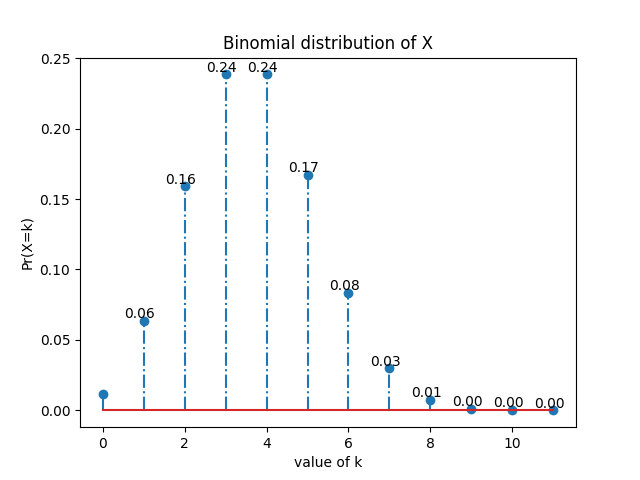
\includegraphics[width=\columnwidth]{binomial/solutions/2/Binomial-stemplot.png}
\caption{Binomial Distribution of  $X$}
\label{binom/2/fig:binom dist}
\end{figure}


%
\item Suppose $X_1,X_2,X_3,X_4$ are i.i.d random variables taking values $1$ and $-1$ with probability $1/2$ each. Then $E\brak{X_1+X_2 +X_3 +X_4}^4$ equals
\begin{multicols}{4}
\begin{enumerate}
    \item $4$
    \item $76$
    \item $16$
    \item $12$
\end{enumerate}
\end{multicols}
\solution
%
\begin{theorem}
    If ${ X_{1},\dots ,X_{n}}$ are i.i.d. random variables, all Bernoulli trials with success probability p, then their sum is distributed according to a binomial distribution with parameters $n$ and $p$
    {\centering
    ${\displaystyle \sum _{k=1}^{n}X_{k}\sim  {B} (n,p)}$
    }
    \label{binom/3/binom_theorem}
    \end{theorem}
    \begin{corollary}
    For a binomial random variable $X$ with parameters $n$ and $p$ and $q=1-p$
    \begin{align}
        E\brak{X}=& n p 
        \\E\brak{X^2}=& n p \brak{n p+q}
        \\E\brak{X^3}=& n p \brak{n^{2} p^{2} + 3 n p q - 2 p q + q}
        \\
        \begin{split}
             E\brak{X^4}=&n p \Bigl(n^{3} p^{3} + 6 n^{2} p^{2} q
            - 11 n p^{2} q  \\& + 7 n p q - 6 p q^{2} + q\Bigr)
        \end{split}
    \end{align}
    \label{binom/3/corolary-momentof-Binom}
    \end{corollary}
    Given that $X_i$ are i.i.d random variable for $i \in \cbrak{1,2,3,4} $ 
    with,
    \begin{align}
        \pr{X_i=+1}=&\frac{1}{2}
        \\\pr{X_i=-1}=&\frac{1}{2}
    \end{align}
    \begin{lemma}
    Let random variables $M_i=\frac{X_i+1}{2}$ then,
    $M_i$ are Bernoulli random variables with $p=0.5$
    \end{lemma}
    \begin{proof}
    \begin{align}
        \pr{M_i=1}=&\pr{X_i=1}=\frac{1}{2}
        \\\pr{M_i=0}=&\pr{X_i=-1}=\frac{1}{2}
    \end{align}
    $\therefore$ $M_i$ are Bernoulli random variables with $p=0.5$
    \end{proof}
    Let assume random variable $Y$ as
    \begin{align}
    Y=\sum_{i=1}^{4}X_i
    \end{align} 
    similarly let 
    \begin{align}
    Z=&\sum_{i=1}^{4}M_i
    \end{align}
    \begin{corollary}
    $Z$  is Binomial random variable , \\from theorem \ref{binom/3/binom_theorem}
    {\centering
    ${\displaystyle Z \sim  {B} (4,0.5)}$
    }
    \label{binom/3/cor-Z_as_binom}
    \end{corollary}
    \begin{align}
    Z=&\sum_{i=1}^{4} \frac{X_i+1}{2}
    \\ Z=&\frac{Y}{2} + 2
    \end{align}
    \begin{align}
        {Y^4}=16{(Z-2)^4}
    \end{align}
    \begin{align}
        {Y^4}=16\brak{Z^4-8z^3+24Z^2-32Z+16}
    \end{align}
    \begin{align}
    \begin{split}
        E\brak{Y^4}=&16\Bigl(E\brak{Z^4}-8E\brak{z^3}
        \\&+24E\brak{Z^2}-32E\brak{Z}+16\Bigr)
    \end{split}    
    \end{align}
    From corollary \ref{binom/3/corolary-momentof-Binom} and  \ref{binom/3/cor-Z_as_binom}
    \begin{align}
        E\brak{Y^4}=&40 &
    \end{align}
    % {\centering
    % $\mbf{\therefore E\brak{X_1+X_2 +X_3 +X_4}^4=40}$
    % }
    

\item The probability that a ticketless traveler is caught during a trip is 0.1. If the traveler makes 4 trips , the probability that he/she will be caught during at least one of the trips is:\\
\begin{enumerate}
    \item $1-(0.9)^4$
    \item $(1-0.9)^4$
    \item $1-(1-0.9)^4$
    \item $(0.9)^4$
\end{enumerate}
\solution
Let $X_i\in\cbrak{0,1}$ represent the ith trip where 1 denotes a ticketless traveller is caught.
Given,
\begin{align}
     \pr{X_i=1}&=p=0.1 \label{dec2015-3:a}
\end{align}
Let,
\begin{align}
    X=\sum_{i=1}^n X_i
\end{align}
where n is the number of trips and X has a binomial distribution.
\begin{align}
    p_X(k)&=
    \begin{cases}
     \comb{n}{k}\,p^K(1-p)^{n-k}, & 0\le k\le n
     \\
    0, & otherwise
    \end{cases}\label{dec2015-3:z}
\end{align}
As he/she makes 4 trips in total, Using \eqref{dec2015-3:a} and
\eqref{dec2015-3:z},
\begin{align}
    \pr{X=0}&=p_X(0)\\
    &=\comb{4}{0}\,p^0(1-p)^4\\
    \pr{X=0}&=(0.9)^4\label{dec2015-3:2}
\end{align}
Then probability of being caught in atleast one trip is,(Using \eqref{dec2015-3:2})
\begin{align}
    \pr{X\ge1}&=1-\pr{X<1}\\
    &=1-\pr{X=0}\label{dec2015-3:1}\\
    &=1-(0.9)^4
\end{align}
%
\item Let X be a binomial random variable with parameters  $\brak{11,\displaystyle{\frac{1}{3}}}$. At which value(s) of k is $\Pr\brak{X = k}$ maximized?\\
\begin{enumerate}
\item k=2
\item k=3
\item k=4
\item k=5
\end{enumerate}
%
\solution
X has a binomial distribution :
\begin{align}
\Pr\brak{X=k} = {\comb{n}{k}}(q)^{n-k}(p)^{k}
\end{align}
Where,
\begin{itemize}
\item n=11
\item $\displaystyle{p=\frac{1}{3}}$
\item $\displaystyle{q=1-p=1-\frac{1}{3}=\frac{2}{3}}$
\end{itemize}
\begin{align}
\Pr\brak{X = k}={\comb{11}{k}}\left(\frac{2}{3}\right)^{11-k}\left(\frac{1}{3}\right)^{k}
\end{align}
For Pr(X = k) to be maximized
\begin{align}
\Pr\brak{X = k}\:\geq\:\Pr\brak{X = k+1}\\
\frac{\Pr\brak{X = k}}{\Pr\brak{X = k+1}}=\frac{{\comb{11}{k}}\left(\frac{2}{3}\right)^{11-k}\left(\frac{1}{3}\right)^{k}}{{\comb{11}{k+1}}\left(\frac{2}{3}\right)^{10-k}\left(\frac{1}{3}\right)^{k+1}}\geq1
\end{align}
\begin{align}
\frac{2(k+1)}{11-k}\geq1\\
\implies k\geq3\label{dec2012-104:0.0.7}\\
\Pr\brak{X = k}\:\geq\:\Pr\brak{X = k-1}\\
\frac{\Pr\brak{X = k}}{\Pr\brak{X = k-1}}=\frac{{\comb{11}{k}}\left(\frac{2}{3}\right)^{11-k}\left(\frac{1}{3}\right)^{k}}{{\comb{11}{k-1}}\left(\frac{2}{3}\right)^{12-k}\left(\frac{1}{3}\right)^{k-1}}\geq1\\
\frac{12-k}{2k}\geq1\\
\implies k\leq4\label{dec2012-104:0.0.10}
\end{align}
From \eqref{dec2012-104:0.0.7} , \eqref{dec2012-104:0.0.10} and since k is an integer\\
$\Pr\brak{X = k}$ is maximized for k=3, k=4\\
Thus options 2) and 3) are correct\\


\end{enumerate}
%
\section{Poisson  Distribution}
\renewcommand{\theequation}{\theenumi}
\renewcommand{\thefigure}{\theenumi}
\renewcommand{\thetable}{\theenumi}
\begin{enumerate}[label=\thesection.\arabic*.,ref=\thesection.\theenumi]
\numberwithin{equation}{enumi}
\numberwithin{figure}{enumi}
\numberwithin{table}{enumi}

\item Let $X_{1}$ and  $X_{2}$ be i.i.d random variables with poisson. Then ($X_{1}+2X_{2}$) is not sufficient because
\begin{enumerate}
    \item{$\pr{X_{1}=1,X_{2}=1 |T=3}$ depends on $\lambda$}\\
    \item{$X_{1}+2X_{2}$ is poisson}\\
     \item{$X_{1}+2X_{2}$ is not poisson}\\
      \item{$\pr{X_{1}=1,X_{2}=1 | T=3}$ is Poisson with parameter one}\\
\end{enumerate}
Where T=($X_{1}+2X_{2}$)
\solution
%\begin{definition}
    Statistic : A statistic is a function T = r($X_{1},X_{2},\dots,X_{n}$) of the random sample $X_{1},X_{2},\dots,X_{n}$.
  \end{definition}
  \begin{definition}
   Sufficient Statistics : A statistic t = T(X) is sufficient for $\theta$ if the conditional probability distribution of data X, given the statistic t = T(X), doesn't depend on the parameter $\theta$.
   \begin{align}
       \pr{\theta \vert T(X)}=\pr{\theta \vert X}
   \end{align}
  \end{definition}
  \begin{theorem}[Factorization theorem]\label{poisson/4/factor}
   : Let $X_{1},X_{2} · · · , X_{n}$ form a random sample from either a continuous
distribution or a discrete distribution for which the pdf or the point mass function is $f(x\vert\theta)$,
where the value of $\theta$ is unknown and belongs to a given parameter space $\Theta$. A statistic
T($X_{1},X_{2} · · · , X_{n}$) is a sufficient statistic for $\theta$ if and only if the joint pdf or the joint point mass
function $f_{n}$(x$\vert\theta$) $X_{1},X_{2} · · · , X_{n}$ can be factorized as follows for all values of $x = (X_{1},X_{2} · · · , X_{n}) \to$
$R^{n}$ and all values of $\theta \in \Theta$:
$f_{n}(x\vert \theta) = u(x)v\brak{T(x), \theta}.$\\
Here the function u may depend on x but does not
depend on $\theta$, and the function v depends on $\theta$ but will depend on the observed value x only through the value of the statistic T(x).
  \end{theorem}
  \begin{lemma} \label{poisson/4/a}
Suppose that $X_{1}$ and $X_{2}$ are i.i.d poisson random variables with parameter $\lambda$, $T=X_{1}+2X_{2}$ does not follow poisson distribution.
\end{lemma}
\begin{proof}
Let $\Phi_{X_{1}}(\omega)$, $\Phi_{2X_{2}}(\omega)$ and  $\Phi_{T}(\omega)$be the characteristic functions of probability density function of random variables $X_{1}$, $2X_{2}$ and T respectively.\\
\begin{align}
    \Phi_{X_{1}}(\omega)=E(e^{i\omega X_{1}})&=\sum_{x=0}^{\infty}\pr{X_{1}=x}e^{i\omega x}\\
                    &=\sum_{x=0}^{\infty}\frac{e^{i\omega x-\lambda}\lambda^{x}}{x!}\\
                    &=e^{-\lambda}\sum_{x=0}^{\infty}\frac{(e^{i\omega}\lambda)^{x}}{x!}\\
                    &=e^{\lambda\brak{e^{i\omega}-1}}
\end{align}
Similarly,
% \begin{multline}
%     \Phi_{2X_{2}}(\omega)=E\brak{e^{i\omega 2X_{2}}}&=\sum_{x=0}^{\infty}\pr{X_{2}=\frac{x}{2}}e^{i\omega x}\\
%                     =\sum_{x=0,2,4....}^{\infty}\frac{\brak{e^{i\omega x-\lambda}}\lambda^{\frac{x}{2}}}{(\frac{x}{2})!}\\
%                     =e^{-\lambda}\sum_{\frac{x}{2}=0,1,2..}^{\infty}\frac{\brak{e^{2i\omega}\lambda}^{\frac{x}{2}}}{(\frac{x}{2})!}\\
%                     =e^{\lambda\brak{e^{2i\omega}-1}}\\
%                     \end{multline}
                    \begin{align}
\Phi_{T}\brak{\omega}&=\Phi_{X_{1}}\brak{\omega}\times\Phi_{2X_{2}}\brak{\omega}\\
 &=e^{\lambda\brak{e^{i\omega}+e^{2i\omega}-2}}\\ 
 &\neq e^{\mu\brak{e^{i\omega}-1}}
 \end{align}
 Hence the characteristic function of T ($\Phi_{T}(\omega)$) is not in the form of the characteristic function of a poisson random variable (for any value of the parameter $\mu$).\\
 \end{proof}
 \begin{lemma}
 Suppose that $X_{1}$ and $X_{2}$ are i.i.d random variables with poisson distribution then T=$X_{1}+2X_{2}$ is not a sufficient statistic.
 \end{lemma}
 \begin{proof}
 Joint p.m.f of $X_{1}$ and $X_{2}$ is,
 \begin{align}
     f_{X_{1}X_{2}}(x_{1},x_{2})&=\frac{e^{-2\lambda}\lambda^{\brak{x_{1}+x_{2}}}}{x_{1}!x_{2}!}\label{poisson/4/a}\\
     &=\frac{1}{x_{1}!x_{2}!}\times\lambda^{T\brak{X_{1},X_{2}}}e^{-2\lambda}\lambda^{-x_{2}}
 \end{align}
 As we can see \eqref{poisson/4/a} cannot be expressed in the form of $u(x)v\brak{T(x), \theta}$\\
 Hence using factorization theorem \ref{poisson/4/factor}, T is not a sufficient statistic. 
 \end{proof}
  \begin{enumerate}
 \item We know T=3 when $(X_{1},X_{2})$ have values (1,1) and (3,0)
  \begin{multline}
\pr{X_{1}=1,X_{2}=1 |T=3}\\&=\frac{\pr{X_{1}=1,X_{2}=1 \cap T=3}}{\pr{T=3}}\\
=\frac{\pr{X_{1}=1,X_{2}=1}}{\pr{X_{1}=1,X_{2}=1}+\pr{X_{1}=3,X_{2}=0}}\\
=\frac{e^{-2\lambda}\lambda^{2}}{e^{-2\lambda}\lambda^{2}+\frac{e^{-3\lambda}\lambda^{3}}{6}}\\
=\frac{6}{6+\lambda}\neq \frac{e^{-1}1^{\lambda}}{\lambda!}
\end{multline}
Hence $\pr{X_{1}=1,X_{2}=1 |T=3}$ depends on $\lambda$ but is not poisson with parameter 1.
$\implies$option 4 is incorrect and option 1 is correct.\\
\item Using lemma $\ref{poisson/4/a}$, $T=X_{1}+2X_{2}$ is not poisson.\\
$\implies$ option 2 is incorrect, option 3 is correct\\

\item Let $X$ be a Poisson random variable with p.m.f
\begin{align}
\label{poisson/1/eq:1}
P(X=k) = 
    \begin{cases} 
      \frac{e^{-\lambda}\lambda^{k}}{k!},& k=0,1,2,...;  \lambda > 0\\
      0 & \text{otherwise}
   \end{cases}
\end{align}
If $Y = X^2 + 3$, then what is $P(Y=y)$ equal to?
\begin{enumerate}[label={(\Alph*)}]
    \item $\frac{e^{-\lambda}\lambda^{\sqrt{y-3}}}{\sqrt{\brak{y-3}}!}$, for $y =$ \cbrak{3,4,7,12,...}
    \item $\frac{e^{-\lambda}\lambda^{-\sqrt{y-3}}}{\sqrt{\brak{3-y}}!}$, for $y =$ \cbrak{3,4,7,12,...}
    \item $\frac{e^{-\lambda}\lambda^{\sqrt{3-y}}}{\sqrt{\brak{3-y}}!}$, for $y =$ \cbrak{4,7,12,...}
    \item $\frac{e^{-\lambda}\lambda^{-\sqrt{3-y}}}{\sqrt{\brak{3-y}}!}$, for $y =$ \cbrak{4,7,12,...}
\end{enumerate}
%
\solution
%
\begin{align}
    Y = X^2 + 3\\
\implies     X = \sqrt{Y - 3}
\end{align}
Substituting $k = \sqrt{y-3}$ in \eqref{poisson/1/eq:1},
\begin{align}
p_Y(y) = 
    \begin{cases} 
      \frac{e^{-\lambda}\lambda^{\sqrt{y-3}}}{\sqrt{\brak{y-3}}!}, & y=3,4,7,12,...\\
      0&\text{otherwise}
   \end{cases}
\end{align}
Hence, the correct option is \brak{A}.
\begin{figure}[hb]
    \centering
    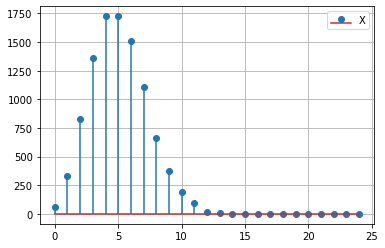
\includegraphics[width=\columnwidth]{poisson/solutions/1/Figures/FigureX.png}
    \caption{Poisson stem plot for X \brak{\lambda = 5}}
    \label{poisson/1/fig:plot1}
\end{figure}
\begin{figure}[hb]
    \centering
    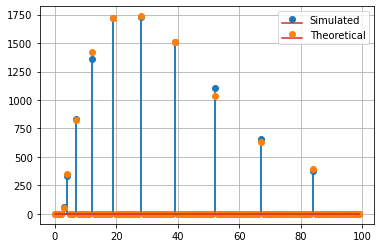
\includegraphics[width=\columnwidth]{poisson/solutions/1/Figures/FigureComp.png}
    \caption{Stem plot for Y (Simulated and Theoretical) \brak{\lambda = 5}}
    \label{poisson/1/fig:plot3}
\end{figure}


\item For $n \geq 1$, let $X_n$ be a Poisson random  variable with mean $n^2$.
 Which of the following are equal to
 $\displaystyle{\frac{1}{\sqrt{2\pi}} \int \limits_2^{\infty} e^{-x^2/2}\,dx}$
\begin{enumerate}
    \item $\lim \limits_{n \to \infty} $ \pr{X_n > (n+1)^2}
    \item $\lim \limits_{n \to \infty} $ \pr{X_n \leqslant (n+1)^2}
    \item $\lim \limits_{n \to \infty} $ \pr{X_n<(n-1)^2}
    \item $\lim \limits_{n \to \infty} $ \pr{X_n<(n-2)^2}
\end{enumerate}
%
\solution
\begin{lemma}
    Let $Y_i$ be a Poisson random variable with mean $1$ for $i$ $\in$ $\brak{1,n^2}$
Then, 
\begin{align}
    \sum \limits_{i}^{n^2} Y_i = X_n   
\end{align}

\end{lemma}
\begin{lemma}
    \begin{align}
         \lim  \limits_{n\to \infty} \frac{X_n-n^2}{n} = \mathcal{N}\brak{0,1}
         \label{poisson/2/central}
    \end{align}
    \label{poisson/2/central/lemma}
\end{lemma}
\begin{proof}
Using the  central limit theorem,
    \begin{align}
        \lim  \limits_{n \to \infty} \frac{Y_1+Y_2+..+Y_{n^2} - n^2}{n} = \mathcal{N}(0,1)
    \end{align}
yielding \eqref{poisson/2/central}.
\end{proof}
\begin{lemma}
    \begin{align}
    Q\brak{2} = \displaystyle{\frac{1}{\sqrt{2\pi}} \int \limits_2^{\infty} e^{-x^2/2}\,dx}
\end{align}
\label{poisson/2/qfunc/lemma}
\end{lemma}
\begin{lemma}
        \begin{align}
            \pr{X_n>k} 
            \\ =& Q\brak{\frac{k-n^2}{n}}
            \label{poisson/2/eq-cdf}
        \end{align}        
        \label{poisson/2/eq-cdf/lemma}
\end{lemma}
\begin{proof}
    For $X \sim \gauss{0}{1}$, using Lemma     \ref{poisson/2/central/lemma},
    \begin{align}
        \pr{X_n>k} 
            =& \pr{X>\frac{k-n^2}{n}}
    \end{align}
    yielding             \eqref{poisson/2/eq-cdf}.
\end{proof}
\begin{lemma}
\begin{align}
    Q\brak{X}=1-Q\brak{-x}
    \label{poisson/2/eq-Qx}
\end{align}
\label{poisson/2/eq-Qx/lemma}
\end{lemma}

% Here, $\mathcal{N}\brak{0,1}$ is normal distribution with unit mean and variance
% Now 
% \begin{align*}
%     \because \,{\frac{1}{\sqrt{2\pi}} \int \limits_{-x}^{\infty} e^{-x^2/2}\,dx}\,=\,{\frac{1}{\sqrt{2\pi}} \int \limits_{-\infty}^x e^{-x^2/2}\,dx}
%     \\ \text{and} \quad \frac{1}{\sqrt{2\pi}} \int \limits_{-\infty}^{\infty} e^{-x^2/2}\,dx\,=1
% \end{align*}
% Also
% \begin{align}
%     \frac{1}{\sqrt{2\pi}} \int \limits_2^{\infty} e^{-x^2/2}\,dx=& Q\brak{2}
% \end{align}
\begin{enumerate}
%\setlength\itemsep{1em}
\item Using Lemma         \ref{poisson/2/eq-cdf/lemma},
\begin{align}
    \lim \limits_{n \to \infty} \pr{X_n > (n+1)^2} =& \lim \limits_{n \to \infty}Q \brak{\frac{(n+1)^2-n^2}{n}}
    \\=&Q\brak{2}
\end{align}
$\mathbf{\therefore}$ \textbf{Option 1 is correct}
\item Using Lemma         \ref{poisson/2/eq-cdf/lemma},
\begin{align}
\begin{split}
    \lim \limits_{n \to \infty} & \pr{X_n \leqslant (n+1)^2}\\ =&1-\lim \limits_{n \to \infty}  \pr{X_n > (n+1)^2}
\end{split}
    \\=&1- \lim \limits_{n \to \infty}Q \brak{\frac{(n+1)^2-n^2}{n}}
    \\=&1- Q \brak{2}
    \\ \ne &  Q\brak{2}
\end{align}
$\mathbf{\therefore}$, from Lemma \ref{poisson/2/qfunc/lemma} \textbf{Option 2 is incorrect}
\item   Using Lemma         \ref{poisson/2/eq-cdf/lemma} and Lemma \ref{poisson/2/eq-Qx/lemma}
\begin{align}
\begin{split}
    \lim \limits_{n \to \infty} & \pr{X_n < (n-1)^2}\\ =&1-\lim \limits_{n \to \infty}  \pr{X_n \geq (n-1)^2}
\end{split}
    \\=&1-\lim \limits_{n \to \infty}Q \brak{\frac{(n-1)^2-n^2}{n}}
    \\=& 1-Q \brak{-2}
    \\=& Q\brak{2}
\end{align}
$\mathbf{\therefore}$ \textbf{Option 3 is also correct}
\item Using Lemma         \ref{poisson/2/eq-cdf/lemma} and Lemma \ref{poisson/2/eq-Qx/lemma},
\begin{align}
   \begin{split}
    \lim \limits_{n \to \infty} & \pr{X_n < (n-2)^2}\\ =&1-\lim \limits_{n \to \infty}  \pr{X_n \geq (n-2)^2}
\end{split}
    \\=&1-\lim \limits_{n \to \infty}Q \brak{\frac{(n-2)^2-n^2}{n}}
    \\=&1- Q \brak{-4}
    \\=& Q\brak{4} < Q \brak{2}
\end{align}
$\mathbf{\therefore}$ \textbf{Option 4 is incorrect}
\end{enumerate}

%
%
\solution
\begin{definition}\label{poisson/3/poisson_process}
    (Poisson Process)\\
    A counting process (number of arrivals from time $0$ to $t$) is called a Poisson process with rate $\lambda$ if
    \begin{enumerate}[label=(\roman*)]
        \item The process has independent increments, and
        \item The number of arrivals in any interval of length $\tau > 0$ has Poisson($\lambda \tau$) distribution.
    \end{enumerate}
    $\therefore$ The distribution of the number of arrivals in any interval depends only on the length of the interval, and not on the exact location of the interval on the real line or on past or future arrivals.
    \end{definition}
    \begin{definition}
        $X$ and $Y$ are Poisson distributions with parameters $\mu_1 = \lambda \, \tau_1 = 2 \times 1$ and $\mu_2 = \lambda \, \tau_2 = 2 \times 5$ respectively. \\
        The pmf (probability mass function) of a Poisson distribution with parameter $\mu$ is given by
        \begin{align}
            p_N(n) &= \dfrac{e^{-\mu}\cdot \mu^{n}}{n!}
        \end{align}
        Hence the pmfs of random variables $X$ and $Y$ are given by:
        \begin{align}
            p_X(x) &= \dfrac{e^{-2}\cdot 2^{x}}{x!}, & \text{for } x=0,1,2,\dots \label{poisson/3/pmf(X)}\\
            p_Y(y) &= \dfrac{e^{-10}\cdot 10^{y}}{y!}, & \text{for } y=0,1,2,\dots \label{poisson/3/pmf(Y)}
        \end{align}
    \end{definition}
        
        \begin{lemma}\label{poisson/3/lemma_X+Y}
            If $X$ and $Y$ are two independent Poisson distributions with parameters $\mu_1$ and $\mu_2$ respectively, then the distribution of $X+Y$ is also Poisson with parameter $\mu_1 + \mu_2$. 
        \end{lemma}
        \begin{proof}
             We have for $k \geq 0$, the probability mass function $p_{X+Y}(k)$ is a convolution of pmfs $p_X(x)$ and $p_Y(y)$: 
        \begin{align}
           p_{X+Y}(k) &= \pr{X+ Y = k} = \pr{Y = k - X}\\
           &= \sum_{i}\pr{Y = k - i| X=i}\times p_X(i)\label{poisson/3/p_(x+y)}
        \end{align}
        As X and Y are independent: 
        \begin{align}
            \pr{Y\! =\! k - i \mid X=i} = \pr{Y\! = \! k - i} = p_Y(k-i)
        \end{align}
        Simplifying \eqref{poisson/3/p_(x+y)}
        \begin{align}
            p_{X+Y}(k) &= \sum_{i=0}^k p_Y(k-i) \times p_X(i)\\
            &= \sum_{i=0}^k e^{-\mu_2}\frac{\mu_2^{k-i}}{(k-i)!}e^{-\mu_1}\frac{\mu_1^i}{i!}\\
            &= e^{-(\mu_1 + \mu_2)}\frac 1{k!}\sum_{i=0}^k \frac{k!}{i!(k-i)!}\,\mu_1^i\,\mu_2^{k-i}\\
            &= e^{-(\mu_1 + \mu_2)}\frac 1{k!}\sum_{i=0}^k {k\choose i}\, \mu_1^i\,\mu_2^{k-i}\\
            p_{X+Y}(k) &= \frac{e^{-(\mu_1 + \mu_2)} \cdot (\mu_1 + \mu_2)^k}{k!}
        \end{align}
        \end{proof}
        \begin{lemma}\label{poisson/3/lemma_X-Y}
            If $X$ and $Y$ are two independent Poisson distributions with parameters $\mu_1$ and $\mu_2$ respectively, then the distribution of $X-Y$ is no longer Poisson, as $X - Y$ will also attain negative values.  More precisely, pmf of $X-Y$ is given by \eqref{poisson/3/pmf(X-Y)}, which is a Skellam distribution.
        \end{lemma}
        \begin{proof}
             We have for $k \in \mathbb{Z}$, the probability mass function $p_{X-Y}(k)$ is a convolution of pmfs $p_X(x)$ and $p_Y(y)$: 
        \begin{align}
           p_{X-Y}(k) &= \pr{X\! -\! Y\! =\! k} = \pr{X\! =\! k\! +\! Y}\\
           &= \sum_{i}\pr{X = k + i| Y = i}\times p_Y(i)\label{poisson/3/p_(x-y)}
        \end{align}
        As X and Y are independent, and the Poisson distribution is zero for negative values of the count, the sum is only taken for those terms where $i \geq 0$ and $i+k\geq 0$. 
        \begin{align}
            p_{X-Y}(k) &= \sum_{i=max(0, -k)}^\infty p_X(k+i) \times p_Y(i)\\
            &=\sum_{i=max(0, -k)}^\infty e^{-\mu_1}\frac{\mu_1^{k+i}}{(k+i)!}e^{-\mu_2}\frac{\mu_2^i}{i!}\\
            &= e^{-(\mu_1 + \mu_2)}\sum_{i=max(0, -k)}^\infty \dfrac{\mu _{1}^{k+i}\mu _{2}^{i}}{i!(k+i)!}\label{poisson/3/pmf(X-Y)}
        \end{align}
        Hence we can see from \eqref{poisson/3/pmf(X-Y)} that X - Y is not a Poisson distribution.\\
        
        \par \textbf{Note: } This result is valid only for independent Poisson distributions. We may have dependent Poisson distributions whose difference is also Poisson. For example let $Z$ be the random variable with distribution $X + Y$, where $X$ and $Y$ are independent Poisson distributions. From lemma \eqref{poisson/3/lemma_X+Y}, Z is Poisson. And, $Z - Y = X$ is also Poisson by definition, as $Z$ is always at least as great as $Y$ ($i.e.$ not independent).\\
        \end{proof}
        
        
    \begin{enumerate}[label=\textbf{(\Alph*)}]
        \item From the definition of Poisson process (Definition \ref{poisson/3/poisson_process}), $X$ and $Y$ are independent. Hence option (A) is \textbf{correct.}\\
        %Alternatively, using memorylessness property for exponential distributions, we can prove that $X$ and $Y$ are independent.
        \item As $X$ and $Y$ are independent Poisson distributions, using lemma \eqref{poisson/3/lemma_X+Y}, $X+ Y$ is a Poisson with parameter $\mu_1 + \mu_2 = 12 \neq 6$. Hence option (B) is \textbf{incorrect.}
        \begin{align}
             p_{X+Y}(k) &= \frac{e^{-(12)} \cdot (12)^k}{k!}\label{poisson/3/pmf(X+Y)}
        \end{align}\\
        \item  As $X$ and $Y$ are independent Poisson distributions, using lemma \eqref{poisson/3/lemma_X-Y}, $X-Y$ is not Poisson. Hence option (C) is \textbf{incorrect.}\\
    %     \begin{figure}[h!]\label{poisson/3/graph_X-Y}
    %     \centering
    %       \includegraphics[width=\columnwidth]{Figures/pmf(X-Y).png}
    %      \caption{$p_{X-Y}(k)$, with $\mu_1=2$ and $\mu_2=10$}
    % \end{figure}
        \item \begin{align}
            \pr{X=0\mid X+Y=12} = \dfrac{\pr{X=0, Y=12}}{\pr{X+Y=12}}
        \end{align}
        As $X$ and $Y$ are independent, and using \eqref{poisson/3/pmf(X)}, \eqref{poisson/3/pmf(Y)}, and \eqref{poisson/3/pmf(X+Y)}, we have:
        \begin{align}
            \pr{X\!=\!0\mid X\!+\!Y\!=\!12} &= \frac{\pr{X\!=\!0} \cdot \pr{Y\!=\!12}}{\pr{X+Y=12}} \\
            &= \frac{\dfrac{e^{-2}\times 2^{0}}{0!} \times \dfrac{e^{-10}\times10^{12}}{12!}}{\dfrac{e^{-12}\times12^{12}}{12!}}\\
            &= \left(\dfrac{5}{6}\right)^{12}
        \end{align}
        Hence option (D) is \textbf{correct.}
    \end{enumerate}
    \textbf{Ans: (A), (D)}

%
\item Suppose customers arrive in a shop according to a Poisson process with rate $4$ per hour. The shop opens at $10:00$ am. If it is given that the second customer arrives at $10:40 $ am, what is the probability that no customer arrived before $10:30 $ am? 
%
    \begin{enumerate}
        \item $\frac{1}{4}$
        \item $e^{-2}$
        \item $\frac{1}{2}$
        \item $e^{\frac{1}{2}}$
    \end{enumerate}
%
%
\solution
\begin{table}[h]
\resizebox{\columnwidth}{!}{
    \begin{tabular}{|c|c|}
    \hline
         Random Variable &  Time at which people arrive\\
         \hline
        $X_p$ & $p=10:00 - 10:30$\\
        $X_q$ & $q=10:30 - 10:40$\\
        $X_r$ & $r=10:00 - 10:40$\\
        $Y$ & $10:40$\\
        \hline
    \end{tabular}
}
    \caption{Random Variables}
    \label{tab:my_label}
\end{table}
We need to find
\begin{align}
    \pr{X_p = 0 | Y = 2} \label{main_eq}
\end{align}
In the world where the $2^{nd}$ person arrives at $10:40$ am the \eqref{main_eq} becomes:
\begin{align}
    &=\frac{\pr{X_p = 0, X_q = 1}}{\pr{X_r = 1}}\\
    &= \frac{\pr{X_p = 0} \times \pr{X_q = 1}}{\pr{X_r = 1}}\label{sub_eq}
\end{align}
The Poisson function distribution for time interval $t$ and rate $\lambda$ for a random variable $X$:
\[
    f_X(x;t) = \frac{(\lambda t)^x \exp{(-\lambda t)}}{x!}
\]
For the time interval $p$:
\begin{align}
    \lambda = 4, t &= 0.5, x= 0\\
    \pr{X_p = 0} &= f_X\brak{0;\frac{1}{2}}\\
    &= e^{-2}\label{eq_1}\\
\end{align}
For the time interval $q$:
\begin{align}
    \lambda = 4, t &= \frac{1}{6},x = 1\\
    \pr{X_q = 1} &= f_X\brak{1; \frac{1}{6}}\\
    &= \frac{2}{3}e^{\frac{-2}{3}} \label{eq_2}
\end{align}
For the time interval $r$:
\begin{align}
    \lambda = 4, t &= \frac{2}{3}, x = 1\\
    \pr{X_r = 1} &= f_X\brak{1; \frac{2}{3}}\\
    &= \frac{8}{3}e^{\frac{-8}{3}} \label{eq_3}
\end{align}
Substituting \eqref{eq_1} \eqref{eq_2} \eqref{eq_3} in \eqref{sub_eq}:
\begin{align}
    \pr{X_p = 0 | Y = 2} = \frac{1}{4}
\end{align}
%
\item Men arrive in a queue according to a Poisson process with rate $\lambda_1$ and women arrive in the same queue according to another Poisson process with rate $\lambda_2$. The arrivals of men and women are independent. The probability that the first person to arrive in the queue is a man is:
\begin{enumerate}
\item $\dfrac{\lambda_1}{\lambda_1+\lambda_2}$
\item $\dfrac{\lambda_2}{\lambda_1+\lambda_2}$
\item $\dfrac{\lambda_1}{\lambda_2}$
\item $\dfrac{\lambda_2}{\lambda_1} $
    
\end{enumerate}
%
\solution
Let $X$ and $Y$ be Poisson random variables, with the values X takes being the number of men joining the queue in an arbitrary time $t$, and the values Y takes being the number of women joining the queue in an arbitrary time $t$.
\begin{align}
    Pr\brak{X=i}&=\frac{\lambda_1^i\cdot e^{-\lambda_1}}{i!}\\
    Pr\brak{Y=i}&=\frac{\lambda_2^i\cdot e^{-\lambda_2}}{i!}
\end{align}
For 2 independent Poisson distributions with means $\lambda_1$ and $\lambda_2$, the simultaneous distribution can be represented by:
\begin{align}
    Pr\brak{X+Y=i}=\frac{(\lambda_1+\lambda_2)^i\cdot e^{-(\lambda_1+\lambda_2})}{i!}
\end{align}
Now we take conditional probability that if only one person entered the queue within a certain time t, then the probability of them being a man and not a woman is given by:
\begin{align}
    Pr\brak{X=1|(X+Y)=1}&=\frac{Pr\brak{(X=1) + (Y=0)}}{Pr\brak{X+Y=1}}\\
\end{align}
Since X and Y are independent, 
\begin{align}
    Pr\brak{X=1|(X+Y)=1}&=\frac{Pr\brak{X=1}\cdot Pr\brak{Y=0}}{Pr\brak{X+Y=1}}\\
    &=\frac{\frac{\lambda_1^1\cdot e^{-\lambda_1}}{1!}\cdot \frac{\lambda_2^0\cdot e^{-\lambda_2}}{0!}}{\frac{(\lambda_1+\lambda_2)^1\cdot e^{-(\lambda_1+\lambda_2})}{1!}}\\
    &=\frac{\lambda_1}{\lambda_1+\lambda_2}
\end{align}
 The probability that the first person to arrive in the queue is a man is option A, i.e $\frac{\lambda_1}{\lambda_1+\lambda_2}$


\end{enumerate}
%
\section{Gaussian  Distribution}
\renewcommand{\theequation}{\theenumi}
\renewcommand{\thefigure}{\theenumi}
\renewcommand{\thetable}{\theenumi}
\begin{enumerate}[label=\thesection.\arabic*.,ref=\thesection.\theenumi]
\numberwithin{equation}{enumi}
\numberwithin{figure}{enumi}
\numberwithin{table}{enumi}

\item Let $U$ and $V$ be two independent zero mean Gaussian random variables of variances $\frac{1}{4}$ and $\frac{1}{9}$ respectively. The probability $\pr{3V \geq 2U}$ is \dots
\\
\solution
From the given information,
\begin{align}
    U &= \gauss{0}{\frac{1}{4}}
    V &= \gauss{0}{\frac{1}{9}}
\end{align}
%
Let $Y = 3V - 2U$.  Then, 
\begin{align}
   \mean{Y} &= 3\mean{V} - 2\mean{U} = 0
\\
\var{Y} &= 3^2\var{V} + 2^2\var{U} = 2
\end{align}
\begin{align}
    \therefore Y = \gauss{0}{2}
\end{align}
Thus, 
\begin{align}
    \pr{3V \geq 2U} &= \pr{3V-2U \geq 0}
    \\
    &= \pr{Y \geq 0} = \frac{1}{2}
\end{align}
$\because$ Y is symmetric about the origin.

%
\item $(X,Y)$ follows bivariate normal distribution $N_2$(0,0,1,1,$\rho$),  -1 $<$ $\rho$ $<$ 1. Then,
\begin{enumerate}
    \item $X+Y$ and $X-Y$ are uncorrelated only if $\rho$ = 0
    \item $X+Y$ and $X-Y$ are uncorrelated only if $\rho$ $<$ 0
    \item $X+Y$ and $X-Y$ are uncorrelated only if $\rho$ $>$ 0
    \item $X+Y$ and $X-Y$ are uncorrelated for all values of $\rho$
\end{enumerate}
\solution
Given that 
\begin{align}
 \vec{M} = \myvec{ X \\ Y}
 \sim  \gauss{\boldsymbol{\upmu}}{\boldsymbol{\Sigma}}
\end{align}
%
where 
%Here, Mean matrix of X and Y is:
\begin{align}
    \boldsymbol{\upmu} &= \myvec{0 \\ 0}
    \\
\boldsymbol{\Sigma} &= \myvec{
            1 & \rho\\
            \rho & 1 
        }
\end{align}
Also, 
\begin{align}
    X+Y &
    = \vec{A}^\top \vec{M}
    \\
    X-Y &
    =\vec{B}^\top \vec{M}
\end{align}
where
\begin{align}
 \vec{A} &= \myvec{1 \\ 1}, 
    \vec{B} &= \myvec{1 \\ -1}
\end{align}
% Defining Covariance in terms of expectation value:
% \begin{align}
%     Cov(X,Y)=& E[(X-\boldsymbol{\upmu}_x)(Y-\boldsymbol{\upmu}_y)] \\
%     =& E[(X-0)(Y-0)]\\
%     =& E(XY)
% \end{align}
Thus, 
\begin{align}
 Cov(X+Y,X-Y) =& \vec{A}^\top \boldsymbol{\Sigma} \vec{B} \\
    % =& \myvec{1 \\ 1}^\top
    % \myvec{
    %         1 & \rho\\
    %         \rho & 1 
    %     }
    %     \myvec{1 \\ -1}\\ 
    % =& \myvec{1+\rho \\ 1+\rho}^\top
    %     \myvec{1 \\ -1}\\
    % =& (1+\rho)-1(1+\rho) \\
    =&   0
\end{align}
% Note that 
% \begin{align}
% Var(X+Y) = Cov(X+Y , X+Y)\\ 
%  Var(X-Y)  = Cov(X-Y , X-Y)
% \end{align}
% Hence,
% \begin{align}
%     Var(X+Y) =&\vec{A^\top} \boldsymbol{\Sigma} \vec{A} \\
%         =& \myvec{1 \\ 1}^\top
%          \myvec{
%             1 & \rho\\
%             \rho & 1 
%         }
%         \myvec{1 \\ 1}\\
%     =& \myvec{1+\rho \\ 1+\rho}^\top
%         \myvec{1 \\ 1}\\
%     =& 1+\rho+1+\rho \\
%     =& 2+2\rho \neq 0
% \end{align}
% \begin{align}
%     Var(X-Y) =& \vec{B^\top} \boldsymbol{\Sigma} \vec{B} \\
%         =& \myvec{1 \\ -1}^\top
%     \myvec{
%             1 & \rho\\
%             \rho & 1 
%         }
%          \myvec{1 \\ -1}\\
%     =& \myvec{1-\rho \\ \rho-1}^\top
%         \myvec{1 \\ -1}\\
%     =& 1-\rho-\rho+1 \\
%     =& 2-2\rho \neq 0
% \end{align}
% So correlation coefficient is:
% \begin{align}
%     \rho(X+Y,X-Y) = \frac{Cov(X+Y,X-Y)}{\sqrt{var(X+Y) \times var(X-Y)}}
%     = 0
% \end{align}
$\therefore$ X+Y and X-Y are uncorrelated irrespective of value of $\rho$ where $\rho \in \brak{-1,1}$.
%$\therefore$ The correct answer is \textbf{option 4}.
%
\item Let $U$ and $V$ be two independent zero mean Gaussian random variables of variances $\frac{1}{4}$ and $\frac{1}{9}$ respectively. The probability $\pr{3V \geq 2U}$ is \dots
\\
\solution
From the given information,
\begin{align}
    U &= \gauss{0}{\frac{1}{4}}
    V &= \gauss{0}{\frac{1}{9}}
\end{align}
%
Let $Y = 3V - 2U$.  Then, 
\begin{align}
   \mean{Y} &= 3\mean{V} - 2\mean{U} = 0
\\
\var{Y} &= 3^2\var{V} + 2^2\var{U} = 2
\end{align}
\begin{align}
    \therefore Y = \gauss{0}{2}
\end{align}
Thus, 
\begin{align}
    \pr{3V \geq 2U} &= \pr{3V-2U \geq 0}
    \\
    &= \pr{Y \geq 0} = \frac{1}{2}
\end{align}
$\because$ Y is symmetric about the origin.

%
\item Let $X_1,X_2,X_3,X_4,X_5$ be a random sample of size 5 from a population having standard normal distribution.If 
$\overline{X}=\frac{1}{5}\sum_{i=1}^5 X_i$ and $T=\sum_{i=1}^5\brak{X_i-\overline{X}}^2$
then $\mean{T^2\overline{X}^2}$ is equal to 
\begin{enumerate}
    \item 3
    \item 3.6
    \item 4.8
    \item 5.2
\end{enumerate} 
\solution
\begin{lemma}
    \label{gauss/3/xy}
Let 
\begin{align}
    \vec{x}=\myvec{X_1\\
             X_2\\
             X_3\\
             X_4\\
             X_5}
, 
             \vec{y}=\myvec{Y_1\\
             Y_2\\
             Y_3\\
             Y_4\\
             Y_5}, 
             \sim \gauss{\vec{0}}{\vec{I}}
             \\
% \end{align}
% and 
% \begin{align}
    \vec{u}&=\myvec{1\\ 1\\ 1\\ 1\\ 1}, 
    \vec{v}=\myvec{1\\ 1\\ 1\\ 1\\ 0}.
\end{align} 
%
Then 
\begin{align}
    \overline{X}&=\frac{1}{5}\vec{u}^{\top}\vec{x}
    \\
    T &= \norm{\vec{v}^{\top}\vec{y}}^2
    \label{gauss/3/T}
\end{align}
where
\begin{align}
\vec{y} &= \vec{P}\vec{x}, 
\\
\vec{M} &= \vec{I}- \frac{1}{5}\vec{1}
\\
&= \vec{P}^{\top}\vec{D}\vec{P}, 
\\
    \vec{D} &=\myvec{1&0&0&0&0\\
                   0&1&0&0&0\\
                   0&0&1&0&0\\
                   0&0&0&1&0\\
                   0&0&0&0&0}
\end{align}
% \begin{align}
% %     \vec{M}&=\myvec{\frac{4}{5}&-1/5&-1/5&-1/5&-1/5\\
% %                    -1/5&\frac{4}{5}&-1/5&-1/5&-1/5\\
% %                    -1/5&-1/5&\frac{4}{5}&-1/5&-1/5\\
% %                    -1/5&-1/5&-1/5&\frac{4}{5}&-1/5\\
% %                    -1/5&-1/5&-1/5&-1/5&\frac{4}{5}}
% \vec{M} = \vec{I}- \frac{1}{5}\vec{1}
%  \end{align}
  and $\vec{1}$ is the all ones matrix.
\end{lemma}
%
\begin{proof}
From  \eqref{gauss/3/mean} and  \eqref{gauss/3/var}, it is easy to verify that 
\begin{align}
       T&=\vec{x}^{\top}\vec{M}\vec{x},
    \vec{M}^2=\vec{M}
    \\
    \implies T&=\vec{x}^{\top}\vec{P}\vec{D}\vec{P}^{\top}\vec{x}\\
    &=\vec{y}^{\top}\vec{D}\vec{y}
\end{align}
yielding     \eqref{gauss/3/T}.  We have used spectral decomposition above.
%
\end{proof}
\begin{lemma}    
    \label{gauss/3/orth}
    $\vec{y}=\vec{P}\vec{x} \sim \gauss{\vec{0}}{\vec{I}}$ if $\vec{P}^{\top}\vec{P} = \vec{I}$.
\end{lemma}
\begin{proof}
    The  moment generating function 
    \begin{align}
        M_{\vec{x}}\brak{\vec{t}}=exp\brak{\vec{t}^{\top}\vec{\mu}+\frac{1}{2}\vec{t}^{\top}\vec{V}\vec{t}}
    \end{align}
    $\because \vec{\mu}=\vec{0}$ and $\vec{V}=\vec{I}$,
    \begin{align}
         M_{\vec{x}}\brak{\vec{t}}=\exp\brak{\frac{1}{2}\vec{t}^{\top}\vec{t}}\label{gauss/3/2.11}
    \end{align}
    Therefore the joint moment generating function of $\vec{y}$ is
    \begin{align}
        M_{\vec{y}}\brak{\vec{t}}&=M_{\vec{x}}\brak{\vec{P}\vec{t}}\\
        &=exp\brak{\frac{1}{2}\vec{t}^{\top}\vec{P}^{\top}\vec{P}\vec{t}}
        \\
        &= M_{\vec{x}}\brak{\vec{t}}
    \end{align}
%    on comparing with $\eqref{gauss/3/2.11}$ we can say $\vec{y}$ has multivariate normal distribution. 
    \end{proof}
    \begin{corollary}
        \label{gauss/3/xbar}
        $\overline{X} \sim \gauss{0}{\frac{1}{5}}$
    \end{corollary}

    \begin{definition}
        \begin{enumerate}
        \item {\em Random Variable:} A random variable X is a real-valued function defined on the "sample space" $\Omega$ (the set of outcomes being studied via probability).
        \item {\em Borel Set:} A random variable X is studied by means of the probabilities that its value lies within various intervals of real numbers (or, more generally, sets constructed in simple ways out of intervals: these are the Borel measurable sets of real numbers).         
        \item {sigma-algebra: }  Corresponding to any Borel measurable set I is the event $X^*(I)$ consisting of all outcomes $\omega$ for which $X(\omega)$ lies in I.
        The sigma-algebra generated by X is determined by the collection of all such events.
        \item {\em Independent random variables: } The naive definition says two random variables X and Y are independent "when their probabilities multiply." That is, when I is one Borel measurable set and J is another, then 
        \begin{multline}
            \pr{X(\omega)\in I , Y(\omega)\in J}\\=\pr{X(\omega)\in I}\pr{Y(\omega)\in J}.
        \end{multline}
        But in the language of events (and sigma algebras) that's the same as
        \begin{multline}
            \pr{\omega \in X^*(I) , \omega \in Y^*(J)}\\=\pr{\omega \in X^*(I)}\pr{\omega \in Y^*J)}.
        \end{multline}
        \item {\em Function of a random variable: }
        \begin{align}
            (f\circ X)(\omega)&=f(X(\omega))
            \\
            (f\circ X)^*(I)&=X^*(f^*(I))
            \label{eq:gauss/3/omega}
        \end{align}
        \end{enumerate}
    
    \end{definition}
    
\begin{lemma}
    Functions of independent random variables are themselves independent.
    \end{lemma}
    \begin{proof}
     Consider now two functions $f,g:\mathbb{R}\rightarrow \mathbb{R}$ and suppose that $f\circ X$ and $g\circ Y$ are random variables. 
    In other words, every event generated by $f\circ X$ (which is on the left) in         \eqref{eq:gauss/3/omega} is automatically an event generated by X (as exhibited by the form of the right hand side). Therefore         \eqref{eq:gauss/3/omega} automatically holds for $f\circ X$ and $g\circ Y$.
    This covers the case of vector-valued random variables as well.
    \end{proof}
    \begin{corollary}
        Let $\vec{y}$ and $\vec{z}$ be two independent normal random vectors. Then $\vec{y}$ and $\vec{\norm{z}}$ are also independent.
    \end{corollary}

    \begin{lemma}
        \label{gauss/3/t2.3}    
        $\vec{A}\vec{x}, \vec{B}\vec{x}$ are  independent  if and only if $\vec{A}\vec{B}^{\top}=0$
        \end{lemma}
        \begin{proof}
        The given vectors are independent $\iff$ 
        \begin{multline}
            \mean{\brak{\vec{A}\vec{x}-\mean{\vec{A}\vec{x}}}\brak{\vec{B}\vec{x}-\mean{\vec{B}\vec{x}}}^{\top}} = 0\\
             \implies \vec{A}\mean{\brak{\vec{x}-\mean{\vec{x}}}\brak{\vec{x}-\mean{\vec{x}}}^{\top}}\vec{B}^{\top} = 0\\
             \implies \vec{A}\var{\vec{x}}\vec{B}^{\top} = 0\\
             \text{or, } \vec{A}\vec{B}^{\top} = 0, \quad \because \var{\vec{x}} = \vec{I}
        \end{multline}        
        \end{proof}
\begin{theorem}    
    $\vec{u}^{\top}\vec{x}$ and $\vec{v}^{\top}\vec{y}$ are independent.
\end{theorem}
\begin{proof}
    From Lemma     \ref{gauss/3/xy}, 
    \begin{align}
        \vec{y} = \vec{P}\vec{x}. 
    \end{align}        
The given statement can be proved  using Lemma         \ref{gauss/3/t2.3} and noting that      
    \begin{align}
        \vec{u}^{\top}\vec{P}^{\top} \vec{v}=0, 
    \end{align}            
\end{proof}
\begin{corollary}    
    $\overline{X} and T$ are independent.
\end{corollary}
    % \begin{conjecture}
    %     \label{l2.1/gauss/3/}
    %     For any vectors $\vec{u}, \vec{v}$, 
    %     \begin{align}
    %        \brak{\vec{u}^{\top}\vec{x}}\brak{\vec{x}^{\top}\vec{v}}=\vec{u}^{\top}\brak{\vec{x}\vec{x}^{\top}}\vec{v}
    %     \end{align}
    % \end{conjecture}
\begin{definition}
    \label{gauss/3/chisq}
    {\em chi-square distribution: } $\norm{\vec{x}}^2$ is said to be chi-square distributed.  If the length of $\vec{x}$ is $k$,
 The mean and variance are given by
 \begin{align}
   \mean{Y}&=k\\
   \var{Y}&=2k
 \end{align}
\end{definition}
From       Corollary  \ref{gauss/3/xbar} and      Definition \ref{gauss/3/chisq},
\begin{align}
    \mean{\overline{X}^2} &= \frac{1}{5}, 
    \\
    \mean{T^2} &=  \var{T}+\brak{\mean{T}}^2\\
    &=24
    \\
    \implies  \mean{T^2\overline{X}^2}=4.8
\end{align}

\item Suppose
$\begin{pmatrix}
X\\
Y
\end{pmatrix}$ is a random vector such that the marginal distribution of $X$ and the marginal distribution of $Y$ are the same and each is normally distributed with mean 0 and variance 1. Then, which of the following conditions imply independence of $X$ and $Y?$
\begin{enumerate}
\item Cov$\brak{X,Y}=0$
\item $aX+bY$ is normally distributed with mean 0 and variance $a^2+b^2$ for all real $a$ and $b$
\item $\pr{X\le 0, Y\le0}=\frac{1}{4}$
\item $E\sbrak{e^{itX+isY}}=E\sbrak{e^{itX}}E\sbrak{e^{isY}}$ for all real $s$ and $t$
\end{enumerate}
%
\solution


An important property of dirac delta function that will be used at multiple ocassions in this solution is
\begin{align}
\displaystyle\int\limits_{-\infty}^{\infty} f(x)\delta(x-a)dx=f(a) \label{dec/2015/109/eq:dirac}
\end{align}
Given $X\sim N\brak{0,1}, Y\sim N(0,1)$
\begin{enumerate}
\item
\begin{align}
Cov(X,Y)=0\\
E\sbrak{XY}-E\sbrak{X}E\sbrak{Y}=0\\
E\sbrak{XY}=0\\
\displaystyle \int\limits_{-\infty}^{\infty} \int\limits_{-\infty}^{\infty}xyf_{XY}(x,y) dxdy=0
\end{align}
This doesn't imply independence. Counter example given below\\
Lets consider a case where $X$ and $Y$ are dependent based on the following relation, $Y$ being independent of $K$
\begin{align}
X=KY \label{dec/2015/109/eq:case}
\end{align}
PMF for $K$ is given as
\begin{align}
p_K(k)=
\begin{cases}
\frac{1}{2} &k=1\\
\frac{1}{2} & k=-1\\
0 & \text{otherwise}
\end{cases}
\end{align}
A simulation is given below, Y is gaussian, then X also follows gaussian
\begin{figure}[!ht]
\centering
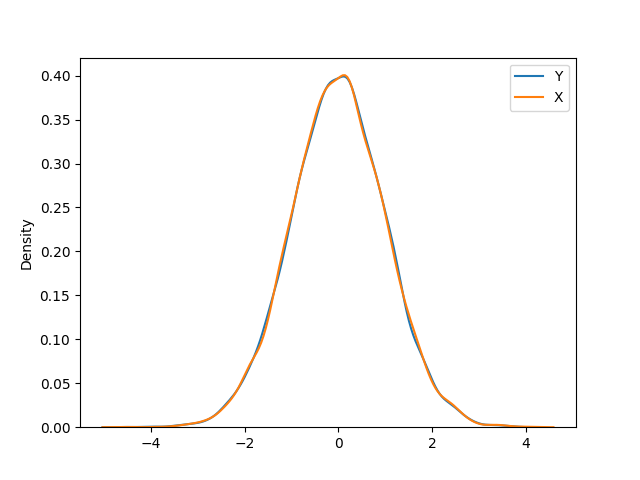
\includegraphics[width=\columnwidth]{solutions/2015/dec/109/figure/fig.png}
\caption{X and Y, if Y is normal}
\label{fig:dec/2015/109/plot}
\end{figure}
Theoretically it can be proved in the following manner,
Since $K$ and $Y$ are independent
\begin{align}
f_X(x)&=\pr{K=1}f_Y(x)+\pr{K=-1}f_Y(-x)\\
&=\frac{1}{2}\brak{f_Y(x)+f_Y(-x)}\\
&=f_Y(x)
\end{align}
Therefore, $X$ follows identical but not independent distribution as $Y$, An alternative proof is given below as a proof for marginal probability\\
Now consider that $X$ is normally distributed, we will establish $Y$ is also normally distributed.
The joint probability distribution is therefore
\begin{align}
f_{XY}(x,y)&=f_{X|Y}(x|y)f_X(x)\nonumber \\
&=f_X(x)\frac{1}{2}(\delta(x+y)+\delta(x-y))\label{dec/2015/109/eq:counter}
\end{align}
The marginal probability distribution function for $X$ is given as
\begin{align}
\int\limits_{-\infty}^{\infty}f_X(x)\frac{1}{2}(\delta(x+y)+\delta(x-y)) dy
\end{align}
Using \eqref{dec/2015/109/eq:dirac}, we get
\begin{align}
\int\limits_{-\infty}^{\infty}f_X(x)\frac{1}{2}(\delta(x+y)+\delta(x-y))dy=f_X(x)
\end{align}
We know that $X\sim N(0,1)$, $f_X(x)$ represents gaussian probability distribution function.\\
Futher, using symmetry of \eqref{dec/2015/109/eq:case}, we can establish that marginal distribution of $Y$ is gaussian. Here is a proof anyways
\begin{align}
f_Y(y)=\int\limits_{-\infty}^{\infty}f_X(x)\frac{1}{2}(\delta(x+y)+\delta(x-y)) dx
\end{align}
Using \eqref{dec/2015/109/eq:dirac}, we get
\begin{align}
f_Y(y)=\frac{1}{2}\brak{f_X(y)+f_X(-y)}=f_X(y)
\end{align}
Since $Y$ has identical probability distribution function, $Y\sim N(0,1)$\\
The covariance is given as
\begin{align}
&Cov(X,Y)=E[XY]-E[X]E[Y]=E[XY]\\
&E[XY]=\int\limits_{-\infty}^{\infty}\int\limits_{-\infty}^{\infty}xyf_{XY}(x,y) dy dx
\end{align}
\begin{align}
=\int\limits_{-\infty}^{\infty}\int\limits_{-\infty}^{\infty}xyf_X(x)\frac{1}{2}(\delta(x+y)+\delta(x-y)) dy dx\\
=\int\limits_{-\infty}^{\infty} xf_X(x)\int\limits_{-\infty}^{\infty}y\frac{1}{2}(\delta(x+y)+\delta(x-y)) dy dx
\end{align}
Using \eqref{dec/2015/109/eq:dirac}
\begin{align}
E[XY]=\int\limits_{-\infty}^{\infty}xf_X(x)\frac{1}{2}(x-x)dx=0
\end{align}
\item
Defining the following matrices/vectors
\begin{table}[h!]
\centering
\begin{tabular}{ |c|c|} 
\hline
\textbf{vector/matrix} & \textbf{expression} \\
\hline&\\[-1em]
$\boldsymbol{Z}$& $\begin{pmatrix} X &Y\end{pmatrix}^\top$\\[2pt]
\hline&\\[-1em]
$\boldsymbol{C}$&$\begin{pmatrix} a &b\end{pmatrix}^\top$  \\[2pt]
\hline&\\[-1em]
$\boldsymbol{\mu}$&$\begin{pmatrix} 0 &0\end{pmatrix}^\top$  \\[2pt]
\hline&\\[-1em]
$\boldsymbol{\Sigma}$&$\begin{pmatrix}1&\rho\\\rho&1\end{pmatrix}$ \\
\hline
\end{tabular}
\caption{vectors/matrices and their expressions}
\label{dec/2015/109/table1}
\end{table}
Given
\begin{align}
\boldsymbol{C^\top Z}\sim N\brak{0,a^2+b^2}
\end{align}
Since this is true for all $a$ and $b$, it is equivalent to $X$ and $Y$ being jointly gaussian
\begin{align}
\boldsymbol{Z}\sim N(\boldsymbol{\mu},\boldsymbol{\Sigma})
\end{align}
For correlated random variables $X$ and $Y$ in bivariate normal distribution, we have
\begin{align}
\sigma_{Z}^2=\displaystyle\sum_{i,j}\Sigma_{ij}\\
a^2+b^2=a^2+b^2+2\rho ab\\
\therefore \rho=0\label{dec/2015/109/eq:rho}
\end{align}
The joint distribution is given as
\begin{align}
f_{\boldsymbol{Z}}(x,y)=\frac{\text{exp}\brak{-\frac{1}{2}\brak{\boldsymbol{z-\mu}}^\top\boldsymbol{\Sigma}^{-1}\brak{\boldsymbol{z-\mu}}}}{\sqrt{(2\pi)^2\abs{\boldsymbol{\Sigma}}}}\\
f_{\boldsymbol{Z}}(x,y)=\frac{\text{exp}\brak{-\frac{1}{2}{\begin{pmatrix} x &y\end{pmatrix}} I_2{\begin{pmatrix} x &y\end{pmatrix}}^\top}}{\sqrt{(2\pi)^2}}
\end{align}
Where $I_2$ is the identity matrix of order 2
\begin{align}
f_{\boldsymbol{Z}}(x,y)=\frac{\text{exp}\brak{-\frac{1}{2}{\begin{pmatrix} x &y\end{pmatrix}} {\begin{pmatrix} x &y\end{pmatrix}}^\top}}{\sqrt{(2\pi)^2}}\\
f_{\boldsymbol{Z}}(x,y)=\frac{\text{exp}\brak{-\frac{1}{2}\brak{x^2+y^2}}}{\sqrt{(2\pi)^2}}=f_X(x)f_Y(y)
\end{align}
$\therefore$ \textbf{Option(2) is correct}, A simulation for bivariate gaussian is given below
\begin{figure}[!ht]
\centering
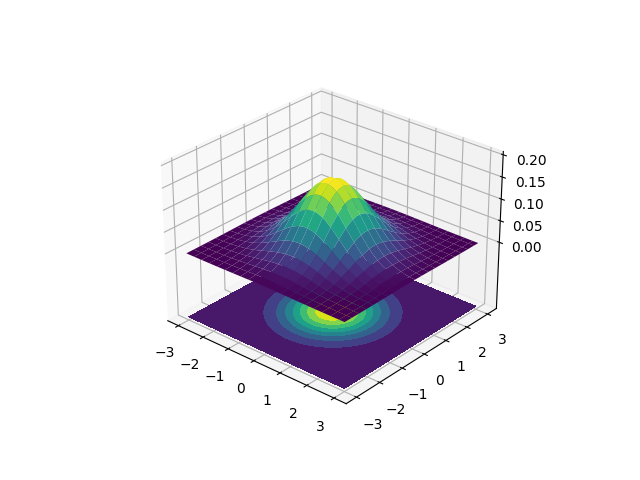
\includegraphics[width=\columnwidth]{solutions/2015/dec/109/figure/plot.png}
\caption{bivariate gaussian while 0 mean vector and identity covariance matrix}
\label{dec/2015/109/plot}
\end{figure}
\item
\begin{align}
\pr{X\le 0, Y\le0}=\frac{1}{4}
\end{align}
This doesn't imply independence, it can be true even for dependent $X$ and $Y$, the counter example is \eqref{dec/2015/109/eq:counter}, the joint probability function is symmetric across all 4 quadrants
\begin{align}
\therefore \pr{X\le 0, Y\le0}=\frac{1}{4}
\end{align}
Alternatively, here is proof 
\begin{align}
\pr{X\le 0}=F_X(0)=\frac{1}{2} \label{dec/2015/109/eq:pr1}
\end{align}
Using \eqref{dec/2015/109/eq:case}
\begin{align}
\pr{Y\le 0|X\le 0}=\frac{1}{2} \label{dec/2015/109/eq:pr2}
\end{align}
Using \eqref{dec/2015/109/eq:pr1} and \eqref{dec/2015/109/eq:pr2}
\begin{align}
\pr{X\le 0, Y\le0}=\frac{1}{4}
\end{align}
\item
\begin{align}
E\sbrak{e^{itX+isY}}=E\sbrak{e^{itX}}E\sbrak{e^{isY}}\\
E\sbrak{e^{itX+isY}}=\varphi_X(t)\varphi_Y(s) \label{dec/2015/109/eq:inde}
\end{align}
The inverse is given as
\begin{align}
f_{XY}(x,y)=\frac{1}{4\pi^2}\displaystyle \int\limits_{-\infty}^{\infty} \int\limits_{-\infty}^{\infty} e^{-itX-isY}E\sbrak{e^{itX+isY}}ds dt
\end{align}
Using \eqref{dec/2015/109/eq:inde}
\begin{align}
f_{XY}(x,y)&=\frac{1}{4\pi^2}\displaystyle \int\limits_{-\infty}^{\infty} \int\limits_{-\infty}^{\infty} e^{-itX-isY}\varphi_X(t)\varphi_Y(s) ds dt\\
&f_{XY}(x,y)=f_X(x)f_Y(y)
\end{align}
$\therefore$ \textbf{Option(4) is correct}
\end{enumerate}




\end{enumerate}
%

\section{Geometric Distribution}
\renewcommand{\theequation}{\theenumi}
\renewcommand{\thefigure}{\theenumi}
\renewcommand{\thetable}{\theenumi}
\begin{enumerate}[label=\thesection.\arabic*.,ref=\thesection.\theenumi]
\numberwithin{equation}{enumi}
\numberwithin{figure}{enumi}
\numberwithin{table}{enumi}


\item Suppose $X$ has density 
%
\begin{align}
f\brak{x|\theta} = \frac{1}{\theta}e^{-x/\theta}, x>0 
\end{align}
Define 
\begin{align}
    Y=k, \quad k\leq X< k+1, \quad k=0,1,2\ldots
\end{align}
%
Then the distribution of $Y$ is
\begin{enumerate}
\begin{multicols}{2}
\setlength\itemsep{0.5em}
    \item Normal
    \item Binomial
    \item Poisson
    \item Geometric
\end{multicols}
\end{enumerate}
\solution
\begin{align}
    \pr{Y=k} &= \pr{k\leq X < k+1}\\
    &= \int_k^{k+1}f\brak{x|\theta}dx\\
    &= \int_k^{k+1}\frac{1}{\theta}e^{-\frac{x}{\theta}}dx\\
    &= \sbrak{-e^{-\frac{x}{\theta}}}_k^{k+1}\\
 &= e^{-\frac{k}{\theta}}\brak{1-e^{-\frac{1}{\theta}}}
 \\
 \implies     \pr{Y=k} &= \brak{1-p}^k p \, k=0,1,2\ldots
\end{align}
%
where
\begin{align}
    p=1-e^{-\frac{1}{\theta}}
\end{align}
Therefore, the distribution of $Y$ is 4) Geometric.




\end{enumerate}




\section{Two Dimensions}
\renewcommand{\theequation}{\theenumi}
\renewcommand{\thefigure}{\theenumi}
\renewcommand{\thetable}{\theenumi}
\begin{enumerate}[label=\thesection.\arabic*.,ref=\thesection.\theenumi]
\numberwithin{equation}{enumi}
\numberwithin{figure}{enumi}
\numberwithin{table}{enumi}

\item Let $ c \in \mathbb{R} $ be a constant. Let $ X, Y$ be random variables with joint probability density function 
\begin{align}
f(x,y)  = 
\begin{cases}
cxy &  0<x<y<1,
\\
0 & \text{ otherwise }
\end{cases}
\label{eq:: joint_pdf}
\end{align}
Which of the following statements are correct ?
\begin{enumerate}
    \item $c = \frac{1}{8}$
    \item $ c= 8$
    \item $X $ and $ Y$ are independent
    \item $\Pr\brak{X= Y} = 0 $
\end{enumerate}
\solution
\begin{enumerate}
    \item False
    \item By definition, 
    \begin{align}
        f_Y\brak{y} &=  \int_{-\infty}^{\infty} f(x,y) \,dx \\
        &= \int_{0}^{y} cxy \,dx \\
        &= cy \brak{\frac{x^2}{2}} \Biggr|_{0}^{y} \\
        &= \frac{ cy^3}{2}
    \end{align}
     \begin{align}
    \label{eq:: pdfy}
    \implies f_Y(y)  = 
    \begin{cases}
    \frac{ cy^3}{2}, &  0<y<1
    \\
    0 & \text{ otherwise. }
    \end{cases}
    \end{align}   
    $\because$ the area under the pdf is 1,  from \eqref{eq:: pdfy},
    \begin{align}
    \implies    \int_{-\infty}^{\infty} f_Y(y) \,dy &= 1 \\
    \implies        \int_{0}^{1} c\frac{y^3}{2} & =1 \\
    \implies    \frac{c}{8} &= 1 \\
    \text{or, }    c & = 8
    \end{align}
%
Also,
% The pdf of Y is 
 \begin{align}
\label{eq:: pdf_y}
f_Y(y)  = 
\begin{cases}
 4y^3 & \text{, if } 0<y<1
\\
0 & \text{, otherwise }
\end{cases}
\end{align}   

\item 
\begin{align}
    f_X\brak{x} &=  \int_{-\infty}^{\infty} f(x,y) \,dy \\
    &= \int_{x}^{1} cxy \,dy \\
    &= cx \brak{\frac{y^2}{2}} \Biggr|_{x}^{1} \\
    &= cx \brak{\frac{1- x^2}{2}}
\end{align}
%
\begin{align}
\label{eq:: pdf_x}
\implies f_X(x)  = 
\begin{cases}
4x \brak{1- x^2}, &  0<x<1
\\
0 & \text{ otherwise }
\end{cases}
\end{align} 
%
From \eqref{eq:: pdf_x} and \eqref{eq:: pdf_y}
\begin{align}
f_X(x) \times f_Y(y) & = 
\begin{cases}
16xy^3 \brak{1- x^2} & \text{, if } 0<x,y<1 
\\
0 & \text{, otherwise }
\end{cases}
\\
  &\neq f(x,y)
\end{align} 
%Since $f(x,y) $ and $ f_X(x) \times f_Y(y) $ are different, random variables 
Hence, $X$ and $Y$ are not independent. 
%Therefore option (3) is not correct. \\
\item
% The marginal PDF of X is given by,
% \begin{align}
% \label{eq:: pdf_x1}
% f_X(x)  = 
% \begin{cases}
% 4x \brak{1- x^2} & \text{, if } 0<x<1
% \\
% 0 & \text{, otherwise }
% \end{cases}
% \end{align} 
% The marginal CDF of X, $ F_X(x)$ is given by,
\begin{align}
    F_X(x) &=  \int_{-\infty}^{x} f_X(x) \,dx \\
    &= \int_{0}^{x} 4x(1-x^2) \,dx \\
     &= \int_{0}^{x} 4x-4x^3 \,dx \\
     & = 2x^2 - 4x^4 \text{ for }  0< x< 1
\end{align}
yielding
\begin{align}
\label{eq:: cdf_x}
F_X(x)  = 
\begin{cases}
0 &  x \le 0
\\
2x^2 - 4x^4    &  0 <x< 1
\\
1 &    x \ge 1
\end{cases}
\end{align}
From \eqref{eq:: cdf_x},
\begin{multline}
    \Pr\brak{Y- \epsilon < X < Y + \epsilon} 
    \\
    = F_X(Y + \epsilon) -  F_X(Y - \epsilon)  
    \\
     = 8\epsilon Y\brak{1 - Y^2 - \epsilon^2}
\end{multline}
upon simplification.  Letting
%
\begin{align}
g(Y)&= 8\epsilon Y(1 - Y^2 - \epsilon^2), \\
    E[g(Y)] &= \int_{-\infty}^{\infty} g(y) f_Y(y) \,dy 
    \\
     & = \int_{0}^{1} (4y^3) (8\epsilon y)(1 - y^2 - \epsilon^2) \,dy 
\end{align}
\begin{multline}
\implies     \Pr\brak{Y- \epsilon < X < Y + \epsilon}     \\
= 32\epsilon \brak{\frac{2- 7\epsilon^2}{35}}
\end{multline}
Now substituting $ \epsilon = 0 $ in the above, 
\begin{align}
    \pr{X =Y}  = 0
\end{align}
\end{enumerate}
%
\item Let $X$ and $Y$ be random variables having the joining probability density function
\begin{align}
f_{XY}(x,y)=
\begin{cases}
\frac{1}{\sqrt{2\pi y}}e^{\frac{-1}{2y}(x-y)^2} & 
\begin{array}{c}
x \in \brak{-\infty,\infty}, 
\\
y \in \brak{0, 1} 
\end{array}
\\
0 &\text{otherwise}
\end{cases}
\label{eq:twoD/2}
\end{align}
The covariance between the random variables X and Y is
\\
%
\solution
%The covariance is defined as
%
\begin{align}
    \cov{XY} = \mean{XY}-\mean{X}\mean{Y}
\end{align}
From \eqref{eq:twoD/2},
%
\begin{align}
    E\brak{XY}=&\int_{0}^{1}\int_{-\infty}^{\infty}xy f_{XY}(x,y)\,dx\,dy\\
    =&\int_{0}^{1}\int_{-\infty}^{\infty}xy\frac{1}{\sqrt{2\pi y}}e^{\frac{-1}{2y}(x-y)^2}\,dx \,dy\\
    =&\int_{0}^{1}y^2 \,dy\\
     \implies E\brak{XY}=&\frac{1}{3} \label{eq:1}
    \end{align}
Y has marginal probability
\begin{align}
    f_Y(y)=&\int_{-\infty}^{\infty}f_{XY}(x,y)\,dx =1\\
    \implies E\brak{Y}=&\frac{1}{2} \label{eq:2}
\end{align}
\begin{align}
 E\brak{X}=&\int_{0}^{1}\int_{-\infty}^{\infty}x f_{XY}(x,y)\,dx\,dy\\
    =&\int_{0}^{1}\int_{-\infty}^{\infty}x\frac{1}{\sqrt{2\pi y}}e^{\frac{-1}{2y}(x-y)^2}\,dx \,dy\\
    =&\int_{0}^{1}y\,dy\\
E\brak{X}=&\frac{1}{2} \label{eq:3} \\
\end{align}
From \eqref{eq:1},\eqref{eq:2},\eqref{eq:3}
\begin{align}
Cov(X,Y)=&E\brak{XY}-E\brak{X}E\brak{Y}\\
       =&\frac{1}{3}-\frac{1}{2}\times \frac{1}{2}\\
Cov(X,Y)=&\frac{1}{12}
\end{align}
\item Let a random variable $X$ follow exponential distribution with mean 2. Define $Y=[X-2|X>2]$. The value of $\pr{Y \geq t}$ is \dots
\\
%
\solution
%Given that, $Y=[X-2|X>2]$
From the given information, 
\begin{align}
\pr{Y \geq t} &= \frac{\pr{X-2 \geq t, X>2}}{\pr{X>2}} 
\\
&= \frac{\pr{X \geq t + 2, X>2}}{\pr{X>2}} 
\label{twoD/3/Eq:1}
\end{align}
$\because  X$ has an exponential distribution with parameter $\lambda = \frac{1}{2}$, 
\begin{align}
	F_X\brak{x} &= \begin{cases} \label{twoD/3/Eq:3}
				1 - e^{-\lambda x}, & \text{if $0 < x< \infty $}\\
				0, & \text{otherwise}
			 \end{cases} 
%	E\brak{x} &= \frac{1}{\lambda} \label{twoD/3/Eq:4}
	\end{align}
	and
	%
\begin{align}
	\pr{X >2} = 1- F_X\brak{2} = e^{-2\lambda}
	\label{twoD/3/Eq:7} 
	\end{align}
%	
Also, 
\begin{align}
	\label{twoD/3/Eq:6}
	\pr{X \geq t+2,X>2} &= 
	\begin{cases}
	\pr{X \geq t+2} & t \ge 0 \\
	\pr{X > 2} & t < 0	
	\end{cases}
		\end{align}
Substituting \eqref{twoD/3/Eq:6} in \eqref{twoD/3/Eq:1},  using 	\eqref{twoD/3/Eq:7} and simplifying,  
\begin{align}
\pr{Y \geq t} = 
\begin{cases}
	 e^{-\frac{t}{2}} & t \ge 0 \\
	1 & t < 0	
	\end{cases}
\end{align}

%
\item Let X and Y be two random variables with joint probability density function
\begin{align*}
    f(x.y)=
    \begin{cases}
    \cfrac{1}{\pi} & 0\le x^2 + y^2 \le 1\\
    0 & otherwise
    \end{cases}
\end{align*}
Which of the following statements are correct?
\begin{enumerate}
    \item
    X and Y are independent.
    
    \item
    $\pr{X>0}=\cfrac{1}{2}$
    
    \item
    E(Y)=0
    
    \item
    Cov(X,Y)=0
\end{enumerate}
%
%
\solution
\begin{enumerate}
    \item 
The marginal PDF of X is given by
\begin{align}
    f_X(x)&=\displaystyle\int\limits_{y=-\infty}^{y=\infty} f_{XY}(x,y) dy\\
          &=\displaystyle\int\limits_{y=-\sqrt{1-x^2}}^{y=\sqrt{1-x^2}}\cfrac{1}{\pi} dy\\
          &=\cfrac{2\sqrt{1-x^2}}{\pi}
\end{align}
The marginal PDF of Y is given by
\begin{align}
    f_Y(x)&=\displaystyle\int\limits_{x=-\infty}^{x=\infty} f_{XY}(x,y) dx\\
          &=\displaystyle\int\limits_{x=-\sqrt{1-y^2}}^{x=\sqrt{1-y^2}}\cfrac{1}{\pi} dx\\
          &=\cfrac{2\sqrt{1-y^2}}{\pi}
\end{align}
Now,
\begin{align}
    f_X(x)\times f_Y(x) &=\cfrac{2\sqrt{1-x^2}}{\pi} \times\cfrac{2\sqrt{1-y^2}}{\pi}\\
    &= \cfrac{4(1-x^2)(1-y^2)}{\pi^2}\\
    &\neq \cfrac{1}{\pi}\\
    &\neq f_{XY}(x,y)
\end{align}
Therefore, X and Y are not independent.\\
\item
Now,
\begin{align}
    \pr{X>0}&=\displaystyle\int\limits_{x=0}^{x=\infty}f_X(x)dx\\
    &=\displaystyle\int\limits_{x=0}^{x=1}\cfrac{2\sqrt{1-x^2}}{\pi} dx\\
    &=\brak{\frac{\arcsin{(x)}+x\sqrt{1-x^2}}{\pi}}_{0}^{1}\\
    &=\cfrac{1}{2}
\end{align}
Therefore, option(2) is correct.\\
\item
Now,
\begin{align}
    E\sbrak{Y}&=\displaystyle\int\limits_{y=-\infty}^{y=\infty}yf_Y(y)dy\\
    &=\displaystyle\int\limits_{y=-1}^{y=1}\cfrac{2y\sqrt{1-y^2}}{\pi}dy\\
    &=\brak{\frac{-2(1-y^2)^{\frac{3}{2}}}{3\pi}}_{-1}^{1}\\
    &=0
\end{align}
Therefore, option(3) is also correct.\\
\item
Now,
\begin{align}
    E\sbrak{XY}&=\displaystyle\int\limits_{x}\displaystyle\int\limits_{y}xyf_{XY}(x,y)dydx\\
    &=\displaystyle\int\limits_{x=-1}^{x=1}\displaystyle\int\limits_{y=-\sqrt{1-x^2}}^{y=\sqrt{1-x^2}}\cfrac{xy}{\pi}dydx\\
    &=\cfrac{x}{\pi} \displaystyle\int\limits_{x=-1}^{x=1}\brak{\cfrac{y^2}{2}}_{-\sqrt{1-x^2}}^{\sqrt{1-x^2}}dx\\
    &=0
\end{align}
Now,
\begin{align}
    Cov(X,Y)&=E\sbrak{XY}-E\sbrak{X}E\sbrak{Y}\\
    &=0-E\sbrak{X}\times0\\
    &=0
\end{align}
Therefore, option(4) is also correct.\\
\end{enumerate}

\item Let X and Y be two random variables satisfying $X\geq 0, Y \geq 0, E(X)=3, Var(X)=9, E(Y)=2$ and $Var(Y)=4$. Which of the following statements are correct?
\begin{enumerate}[label=\Alph*)]
    \item $0\leq Cov(X,Y)\leq 4$
    \item $E(XY)\leq 3$
    \item $Var(X+Y)\leq 25$
    \item $E(X+Y)^2\geq 25$
\end{enumerate}
%
\solution
\begin{equation}
    E(X^2) = Var(X)+(E(X))^2 = 18
\end{equation}
Similarly,
\begin{equation}
    E(Y^2) = Var(Y)+(E(Y))^2 = 8
\end{equation}
We can use the Covariance inequality for this question,
\begin{equation}
  ({Cov(X,Y)})^2\leq Var(X)Var(Y)
\end{equation}
The proof of this inequality is as shown,
\begin{align}
\nonumber    Var\brak{\dfrac{X}{\sigma_X}\pm\dfrac{Y}{\sigma_Y}} &= Var\brak{\dfrac{X}{\sigma_X}}+Var\brak{\dfrac{\pm Y}{\sigma_Y}}\\[6pt]
    &+2Cov\brak{\dfrac{X}{\sigma_X},\dfrac{\pm Y}{\sigma_Y}}\\
\nonumber    &=\dfrac{1}{{\sigma_X}^2}Var(X)+\dfrac{1}{{\sigma_Y}^2}Var(Y)\\[6pt]
    &+2 Cov\brak{\dfrac{X}{\sigma_X},\dfrac{\pm Y}{\sigma_Y}}\\[6pt]
    &=2\pm2\dfrac{Cov(X,Y)}{{\sigma_X}{\sigma_Y}}
\end{align}
Since Variance is always positive,
\begin{align}
    Var\brak{\dfrac{X}{\sigma_X}\pm\dfrac{Y}{\sigma_Y}}\geq 0
    \\[6pt]
    2\pm2\dfrac{Cov(X,Y)}{{\sigma_X}{\sigma_Y}} \geq 0
    \\[6pt]
    1\pm1\dfrac{Cov(X,Y)}{{\sigma_X}{\sigma_Y}}\geq 0
    \\[6pt]
    \abs{({Cov(X,Y)})}\leq (\sigma_X)(\sigma_Y)
    \\
    ({Cov(X,Y)})^2\leq Var(X)Var(Y)
\end{align}
\begin{enumerate}
\item
Substituting values of variance we get,
\begin{equation}\label{june/2018/104cov}
    -6\leq{Cov(X,Y)}\leq 6
\end{equation}
\textbf{Therefore, option A is incorrect}.\\
\item
From equation \eqref{june/2018/104cov},
\begin{equation}
    {Cov(X,Y)}=E(XY)-E(X)E(Y)
\end{equation}
\begin{align}
    -6\leq E(XY)-E(X)E(Y)\leq 6
\end{align}
\begin{equation}\label{june/2018/104exy}
    0\leq E(XY)\leq12
\end{equation}
Also, if X and Y are independent,
\begin{equation}
    E(XY)=E(X)E(Y)=6
\end{equation}
\textbf{Therefore, Option B is incorrect.}\\
\item
Now,
\begin{align}
    Var(X+Y)&=Var(X)+Var(Y)+2Cov(X,Y)\\
    &=13+2Cov(X,Y)
\end{align}
From equation \eqref{june/2018/104cov},
\begin{equation}
    1\leq Var(X+Y)\leq 25
\end{equation}
\textbf{Therefore, Option C is correct.}\\
\item
Now,
\begin{align}
    E(X+Y)^2 &= E(X^2)+E(Y^2)+2E(XY)\\
    E(X+Y)^2 &= 26+2E(XY)
\end{align}
From equation \eqref{june/2018/104exy},
\begin{equation}
    26\leq E(X+Y)^2\leq50
\end{equation}
\textbf{Therefore, Option D is correct.}\\
\end{enumerate}
%
\item The joint probability density function of (X,Y) is
\begin{equation}
    f(x,y) =
    \begin{cases}
        6(1-x) & if \hspace{0.3cm}0<y<x ,0<x<1\label{0.0.1} \\
        0      & \text{otherwise}
    \end{cases}
\end{equation}
Which among the following are correct?
\begin{enumerate}\itemsep0.3cm
    \item X and Y are not independent
    \item
          $ f_Y(y) =
              \begin{cases}
                  3\brak{y-1}^{2} & if \hspace{0.3cm}0<y<1 \\
                  0               & \text{otherwise}
              \end{cases}$
    \item X and Y are independent
    \item $ f_Y(y) =
              \begin{cases}
                  3\brak{\displaystyle{y-\frac{1}{2}{y}^2}} & if \hspace{0.3cm}0<y<1 \\
                  0                                         & \text{otherwise}
              \end{cases}$
\end{enumerate}
%
\solution
Given joint probability density function of X and Y, marginal probability density functions are as follows:
\begin{align}
    f_X(x) = \int_{-\infty}^{\infty} f(x,y) dy \\[0.4cm]
    f_Y(y) = \int_{-\infty}^{\infty} f(x,y) dx
\end{align}
Calculating $f_X(x)$
\begin{align}
    f_X(x) = & \int_{-\infty}^{\infty} f(x,y) dy \\
    =        & \int_{0}^{x} 6(1-x) dy            
\end{align}
\begin{align}
    f_X(x) =
    \begin{cases}
        6x(1-x) & 0<x<1     \label{june2016-104:0.0.6}\\
        0       & otherwise
    \end{cases}
\end{align}
Calculating $f_Y(y)$
\begin{align}
    f_Y(y) = & \int_{-\infty}^{\infty} f(x,y) dx \\
    =        & \int_{y}^{1} 6(1-x) dx\\
    =        & 6x -3{x}^2 \big|_{y}^{1}\\
    =        & 3 - 6y + 3y^{2}\\
    =        & 3{(y-1)}^{2}      
\end{align}
\begin{align}
    f_Y(y) =
    \begin{cases}
        3{(y-1)}^{2}  & 0<y<1     \label{june2016-104:0.0.12}\\
        0       & otherwise
    \end{cases}
\end{align}
To check whether X and Y are independent, we calculate $f_X(x) \times f_Y(y)$. From \eqref{june2016-104:0.0.6} and \eqref{june2016-104:0.0.12}
\begin{align}
    f_X(x) \times f_Y(y) = &
    \begin{cases}
        18x(1-x){(y-1)}^{2}  \\ \hspace{1.2cm}0<x<1,0<y<1\\
        0 \hspace{1cm} \text{otherwise}
    \end{cases}\\
    \neq & f(x,y)
\end{align}
Since f(x,y) and $f_X(x)\times f_Y(y)$ are different, random variables X and Y are not independent.
\begin{center}
    Options 1 and 2 are correct
\end{center}
%
\item Suppose that $(X,Y)$ has a joint probability distribution with the marginal distribution of $X$ being N(0,1) and $E(Y|X=x)=x^3$ for all $x \in R$. Then, which of the following statements are true?
\begin{enumerate}
    \item Corr$(X,Y) = 0$
    \item Corr$(X,Y) > 0$
    \item Corr$(X,Y) < 0$
    \item X and Y are independent
\end{enumerate}
\solution
The following result shall be useful later. For $n \in N$
\begin{align}
    \int_{-\infty}^{\infty} \dfrac{x^n e^{\frac{-x^2}{2}}}{\sqrt{2\pi}}dx = 
    \begin{cases}
    0 & n\; is\; odd\\
    (n-1)\times...\times3\times1 & n\; is\; even
    \end{cases}
\end{align}
The proof for the above can be found at the end of the solution.
\begin{align}
    Corr(X,Y) = \cfrac{\sigma_{XY}^2}{\sigma_X\sigma_Y}
    \label{dec2015-108:correlationofxy}
\end{align}
We know $X \sim N(0,1)$. Thus,
\begin{align}
    f_X(x) &= \dfrac{e^{\frac{-x^2}{2}}}{\sqrt{2\pi}}\\
    E(X) &= 0\\
    \sigma_X^2 &= 1
\end{align}
\begin{align}
    \sigma_Y^2 = E(Y^2) - E(Y)^2
    \label{dec2015-108:varianceofy}
\end{align}
\begin{align}
    E(Y) &= \int_{-\infty}^{\infty}E(Y|X=x)f_X(x)dx\\
         &= \int_{-\infty}^{\infty}\dfrac{x^3 e^{\frac{-x^2}{2}}}{\sqrt{2\pi}}dx\\
         &= 0
\end{align}
\begin{align}
    E(Y^2) &= \int_{-\infty}^{\infty}E(Y^2|X=x)f_X(x)dx\\
           &= \int_{-\infty}^{\infty}\dfrac{x^6 e^{\frac{-x^2}{2}}}{\sqrt{2\pi}}dx\\
           &= 15
\end{align}
Substituting in \eqref{dec2015-108:varianceofy}
\begin{align}
    \sigma_Y^2 = 15
\end{align}
\begin{align}
    \sigma_{XY}^2 = E(XY) - E(X)E(Y)
    \label{dec2015-108:covarianceofxy}
\end{align}
\begin{align}
    E(XY) &= \int_{-\infty}^{\infty}E(XY|X=x)f_X(x)dx\\
          &= \int_{-\infty}^{\infty}E(xY|X=x)f_X(x)dx\\
          &= \int_{-\infty}^{\infty}xE(Y|X=x)f_X(x)dx\\
          &= \int_{-\infty}^{\infty}\dfrac{x^4 e^{\frac{-x^2}{2}}}{\sqrt{2\pi}}dx\\
          &= 3
\end{align}
Substituting in \eqref{dec2015-108:covarianceofxy}
\begin{align}
    \sigma_{XY}^2 = 3
\end{align}
Substituting in \eqref{dec2015-108:correlationofxy}
\begin{align}
    Corr(X,Y) = \cfrac{3}{\sqrt{15}} > 0
\end{align}
Since $Corr(X,Y) \ne 0$, X and Y are dependent. Thus option 2 is the only correct option.
\textbf{Proof for the integral:}
If n is odd, $\dfrac{x^n e^{\frac{-x^2}{2}}}{\sqrt{2\pi}}$ is an odd function, thus
\begin{align}
    \int_{-\infty}^{\infty} \dfrac{x^n e^{\frac{-x^2}{2}}}{\sqrt{2\pi}}dx = 0
\end{align}
If n is even, 
\begin{align}
    \int_{-\infty}^{\infty} \dfrac{x^n e^{\frac{-x^2}{2}}}{\sqrt{2\pi}}dx = \int_{-\infty}^{\infty} (x^{n-1}) (\dfrac{x e^{\frac{-x^2}{2}}}{\sqrt{2\pi}})dx
\end{align}
Using integration by parts,
\begin{multline}
    \int_{-\infty}^{\infty} \dfrac{x^n e^{\frac{-x^2}{2}}}{\sqrt{2\pi}}dx = \left(x^{n-1}\int \dfrac{x e^{\frac{-x^2}{2}}}{\sqrt{2\pi}}dx\right)\biggr \vert_{-\infty}^{\infty}\\
       - (n-1)\int_{-\infty}^{\infty}x^{n-2}\left(\int \dfrac{x e^{\frac{-x^2}{2}}}{\sqrt{2\pi}}dx\right) dx
\end{multline}
\begin{align}
    &= \left(x^{n-1}(-\dfrac{e^{\frac{-x^2}{2}}}{\sqrt{2\pi}})\right)\biggr \vert_{-\infty}^{\infty}
           - (n-1)\int_{-\infty}^{\infty}x^{n-2}(-\dfrac{e^{\frac{-x^2}{2}}}{\sqrt{2\pi}}) dx\\
    &= (n-1)\int_{-\infty}^{\infty} \dfrac{x^{n-2} e^{\frac{-x^2}{2}}}{\sqrt{2\pi}}dx\\
    &= (n-1)(n-3)\int_{-\infty}^{\infty} \dfrac{x^{n-4} e^{\frac{-x^2}{2}}}{\sqrt{2\pi}}dx\\
    &= (n-1)\times...\times3\times1\int_{-\infty}^{\infty} \dfrac{x^0 e^{\frac{-x^2}{2}}}{\sqrt{2\pi}}dx\\
    &= (n-1)\times...\times3\times1
\end{align}
%
%
\item  Consider the quadratic equation $x^2+2U x+V=0$ where $U$ and $V$ are chosen independently and randomly from $\{1,2,3\}$ with equal probabilities. Then probability that the equation has both roots real
\begin{enumerate}
    \item $\frac{2}{3}$
    \item $\frac{1}{2}$
    \item $\frac{7}{9}$
    \item $\frac{1}{3}$
\end{enumerate}
%
\solution
Let $U\in\{1.2,3\}$ and $V\in\{1,2,3\}$
\begin{table}[h!]
\centering
\caption{Probability of selecting values for $U$}
\resizebox{\columnwidth}{!}{
  \begin{tabular}{||c|c|c|c||}
    \hline
    $k$ & $1$ & $2$ & $3$\\
    \hline
    \hline
    $\pr{U=k}$ & $1/3$ & $1/3$ & $1/3$\\
    \hline
  \end{tabular}
}
\label{june2013-60:Table1}
\end{table}
\begin{table}[h!]
\centering
\caption{Probability of selecting values for $V$}
\resizebox{\columnwidth}{!}{
  \begin{tabular}{||c|c|c|c||}
    \hline
    $k$ & $1$ & $2$ & $3$\\
    \hline
    \hline
    $\pr{V=k}$ & $1/3$ & $1/3$ & $1/3$\\
    \hline
  \end{tabular}
}
\label{june2013-60:Table2}
\end{table}
For $x^2+2U x+V=0$ to have real roots,
\begin{align}
    b^2-4ac\geq0\\
    \brak{2U}^2-4\brak{1}\brak{V}\geq0\\
    U^2\geq V
\end{align}
\begin{align}
    \pr{U^2\geq V}=1-\pr{U^2<V}
\end{align}
The possible pairs \brak{U,V} for \pr{U^2<V},
\vspace{0.00001in}
\begin{table}[h!]
\centering
\caption{Table for \pr{U^2<V}}
\resizebox{\columnwidth}{!}{
  \begin{tabular}{||c|c||}
    \hline
    $\brak{U,V}$ for $U^2<V$ & Probability\\
    \hline
    \hline
    $\brak{1,2}$ & \pr{U=1}\pr{V=2}=1/9\\
    \hline
    $\brak{1,3}$ & $\pr{U=1}\pr{V=3}=\frac{1}{9}$\\
    \hline
    \hline
    Total & $\pr{U^2<V}=\frac{2}{9}$\\
    \hline
  \end{tabular}
}
\label{june2013-60:Table3}
\end{table}
\begin{align}
    \pr{U^2\geq V}=1-\frac{2}{9}\\
    \pr{U^2\geq V}=\frac{7}{9}
\end{align}
Hence, Option 3 is correct.


\end{enumerate}
%
\section{Integral Transforms}
\renewcommand{\theequation}{\theenumi}
\renewcommand{\thefigure}{\theenumi}
\renewcommand{\thetable}{\theenumi}
\begin{enumerate}[label=\thesection.\arabic*.,ref=\thesection.\theenumi]
\numberwithin{equation}{enumi}
\numberwithin{figure}{enumi}
\numberwithin{table}{enumi}


%
\item X and Y are independent random variables each having the density
\begin{align}
    f(t) = \displaystyle\frac{1}{\pi} \frac{1}{1+{t}^2} -\infty < t < +\infty
\end{align}
Then the density function of $\displaystyle\frac{X+Y}{3}$ for \\$-\infty <$ t $< +\infty$ is\bigskip
    \begin{enumerate}\itemsep0.5cm
        \item $\displaystyle\frac{6}{\pi} \frac{1}{4+9{t}^2}$
        \item $\displaystyle\frac{6}{\pi} \frac{1}{9+4{t}^2}$
        \item $\displaystyle\frac{3}{\pi} \frac{1}{1+9{t}^2}$
        \item $\displaystyle\frac{3}{\pi} \frac{1}{9+{t}^2}$
    \end{enumerate}

%
\solution
Let us consider the random variables X and Y.
    The Characteristic function of the probability density $f(t)$ is
    \begin{align}
        g(w) =\hspace{0.2cm} & \int_{-\infty}^{\infty}  f(t) {e}^{iwt} dt                                         \\[0.2cm]
        =\hspace{0.2cm}      & \int_{-\infty}^{\infty}  \displaystyle\frac{1}{\pi} \frac{1}{1+{t}^2} {e}^{iwt} dt \\[0.2cm]
        =\hspace{0.2cm}      & e^{-\abs{w}}\hspace{0.2cm}, -\infty<w<\infty
    \end{align}
    The product of the Characteristic function of \\probability density of X and Y is
    \begin{align}
        h(w) = g_1(w) \times g_2(w) = {e}^{-2\abs{w}}
    \end{align}
    To get the probability density of X+Y, we find the inverse characteristic function of h(w). But since there is a one to one correspondence between a function and its fourier transform and
$h(w) = g(2w)$
    \begin{align}
        F_{X+Y}(t) =\hspace{0.2cm} & \frac{1}{2}f\brak{\frac{t}{2}}                                        \\[0.2cm]
        =\hspace{0.2cm}            & \frac{1}{2\pi} \frac{4}{4+{t}^2} \hspace{0.2cm},-\infty<t<\infty
    \end{align}
    We know that if a random variable M has a\\probability density $f_M(x)$, then the probability \\density of random variable kM is
    \begin{align}
        f_{kM}\brak{x} = \frac{1}{\abs{k}} f_M\brak{\frac{x}{\abs{k}}}
    \end{align}
    Probability density of $Z = \displaystyle\frac{X+Y}{3}$ given $F_{X+Y}(t)$ is
\begin{align}
    F_{Z}(t) = & 3\times \displaystyle f_{X+Y}(3t) \\
    =          & \frac{6}{\pi} \frac{1}{4+9{t}^2}
\end{align}

\item Suppose X and Y are independent and identically distributed random variables and let $Z = X + Y$. Then the distribution of $Z$ is in the same family as that of $X$ and $Y$ if X is
\begin{table}[h]
\setlength{\tabcolsep}{30pt}
    \begin{tabular}{ll}
         1) Normal  & 2) Exponential  \\
         3) Uniform & 4) Binomial
    \end{tabular}
\end{table}
%
\solution


\begin{enumerate}[label = \arabic*)]
    \item Let X and Y be independent and identically distributed normal random variables. Then the characteristic function of X and Y is given by
    \begin{equation}
        \Phi_X(\omega) = e^{j\eta\omega - \sigma^2\omega^2/2}
    \end{equation}
    The characteristic function of Z is given by
    \begin{align}
        \Phi_Z(\omega) &= \Phi_X^2(\omega)\\
                       &= e^{2j\eta\omega - \sigma^2\omega^2}
    \end{align}
    Thus Z is a normal random variable with parameters $2\eta$ and $2\sigma^2$. Thus option (1) is correct.
    \item Let X and Y be independent and identically distributed exponential random variables. Then the characteristic function of X and Y is given by
    \begin{equation}
        \Phi_X(\omega) = \dfrac{\lambda}{1-j\omega}
    \end{equation}
    The characteristic function of Z is given by
    \begin{align}
        \Phi_Z(\omega) &= \Phi_X^2(\omega)\\
                       &= \dfrac{\lambda^2}{(1-j\omega)^2}
    \end{align}
    Thus Z is not an exponential random variable. Therefore option (2) is wrong.
    \item Let X and Y be independent and identically distributed uniform random variables such that X, Y $\sim$ U(a,b). Then the characteristic function of X and Y is given by
    \begin{equation}
        \Phi_X(\omega) = \dfrac{e^{jb\omega} - e^{ja\omega}}{j\omega(b-a)}
    \end{equation}
    The characteristic function of Z is given by
    \begin{align}
        \Phi_Z(\omega) &= \Phi_X^2(\omega)\\
                       &= -\dfrac{(e^{jb\omega} - e^{ja\omega})^2}{\omega^2(b-a)^2}
    \end{align}
    Thus Z is not a uniform random variable. Thus option (3) is wrong.
    \item Let X and Y be independent and identically distributed binomial random variables. Then the characteristic function of X and Y is given by
    \begin{equation}
        \Phi_X(\omega) = (pe^{j\omega}+q)^n
    \end{equation}
    The characteristic function of Z is given by
    \begin{align}
        \Phi_Z(\omega) &= \Phi_X^2(\omega)\\
                       &= (pe^{j\omega}+q)^{2n}
    \end{align}
    Thus Z is a binomial random variable with parameter 2n. Thus option (4) is correct.
\end{enumerate}
The following figures show the experimental distributions for Z in each case. The simulation length was kept one million.
\begin{figure}[!ht]
\centering
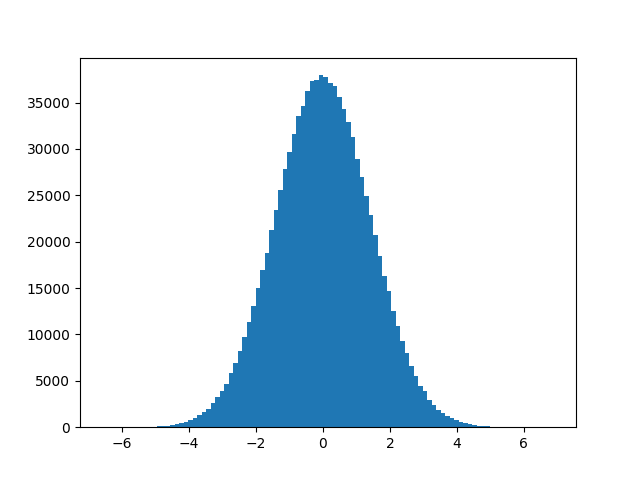
\includegraphics[width=\columnwidth]{solutions/2016/june/107/figures/norm.png}
\caption{Z when X is standard normal}
\label{june2016-107:fig:normal}
\end{figure}
\begin{figure}[!ht]
\centering
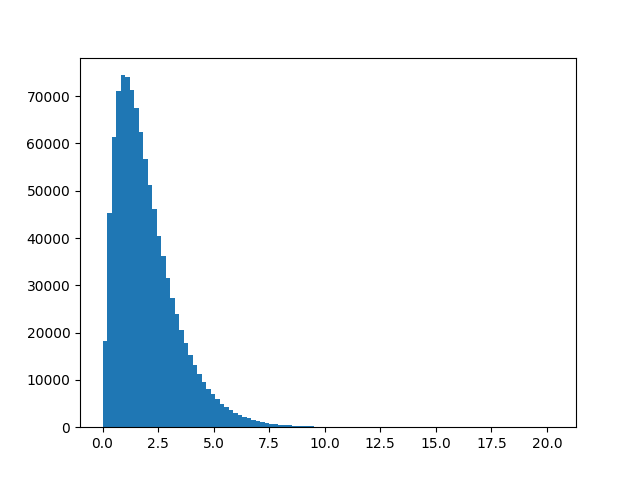
\includegraphics[width=\columnwidth]{solutions/2016/june/107/figures/expon.png}
\caption{Z when X is exponential with $\lambda = 1$}
\label{june2016-107:fig:exponential}
\end{figure}
\begin{figure}[!ht]
\centering
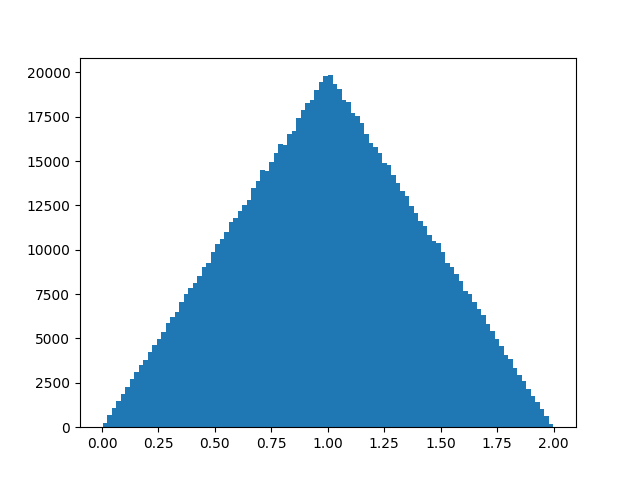
\includegraphics[width=\columnwidth]{solutions/2016/june/107/figures/uniform.png}
\caption{Z when X $\sim$ U(0,1)}
\label{june2016-107:fig:uniform}
\end{figure}
\begin{figure}[!ht]
\centering
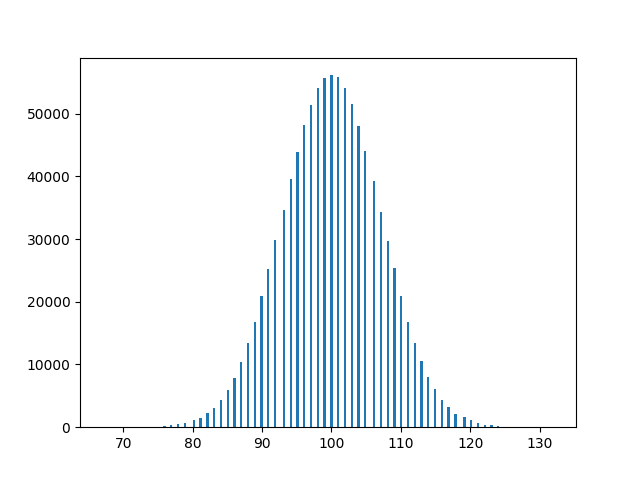
\includegraphics[width=\columnwidth]{solutions/2016/june/107/figures/binom.png}
\caption{Z when X $\sim$ B(100,0.5)}
\label{june2016-107:fig:binomial}
\end{figure}


\item  $N,A_1,A_2\cdots$ are independent real valued random variables such that 
    \begin{align}
        \pr{N=k}=(1-p)p^k,k=0,1,2,3\cdots
    \end{align}
    where $0<p<1$ and $\{A_i:i=1,2,\cdots\}$ is a sequence of independent and identically distributed bounded random variables. Let 
    \begin{align}
        X(w) = 
        \begin{cases}
        0  & \text{if } N(w)=0\\
        \sum_{j=1}^{k} A_j & \text{if } N(w)=k,k=1,2,3\cdots 
        \end{cases}
    \end{align}
    Which of the following are necessarily correct?\\
    \begin{enumerate}
        \item $X$ is a bounded random variable. 
        \item Moment generating function $m_X$ of $X$ is
        \begin{align}
            m_X(t)=\dfrac{1-p}{1-pm_A(t)}, t\in \mathbb{R},
        \end{align}
        where $m_A$ is moment generating function of $A_1$.
        \item Characteristic function $\varphi_X$ of $X$ is
        \begin{align}
            \varphi_X(t)=\dfrac{1-p}{1-p\varphi_A(t)},t\in \mathbb{R},
        \end{align}
        where $\varphi_A$ is the characteristic function of $A_1$.
        \item $X$ is symmetric about 0.
    \end{enumerate}

\end{enumerate}

\section{Markov Chain}
\renewcommand{\theequation}{\theenumi}
\renewcommand{\thefigure}{\theenumi}
\renewcommand{\thetable}{\theenumi}
\begin{enumerate}[label=\thesection.\arabic*.,ref=\thesection.\theenumi]
\numberwithin{equation}{enumi}
\numberwithin{figure}{enumi}
\numberwithin{table}{enumi}


\item \textbf{Step 1.} Flip a coin twice.\\
\textbf{Step 2.} If the outcomes are (TAILS, HEADS) then output Y and stop.\\
\textbf{Step 3.} If the outcomes are either (HEADS, HEADS) or (HEADS, TAILS), then output N and stop.\\
\textbf{Step 4.} If the outcomes are (TAILS, TAILS), then go to Step 1.\\
The probability that the output of the experiment is Y is (upto two decimal places)......
%
\solution
\begin{figure}[!ht]
  \centering
  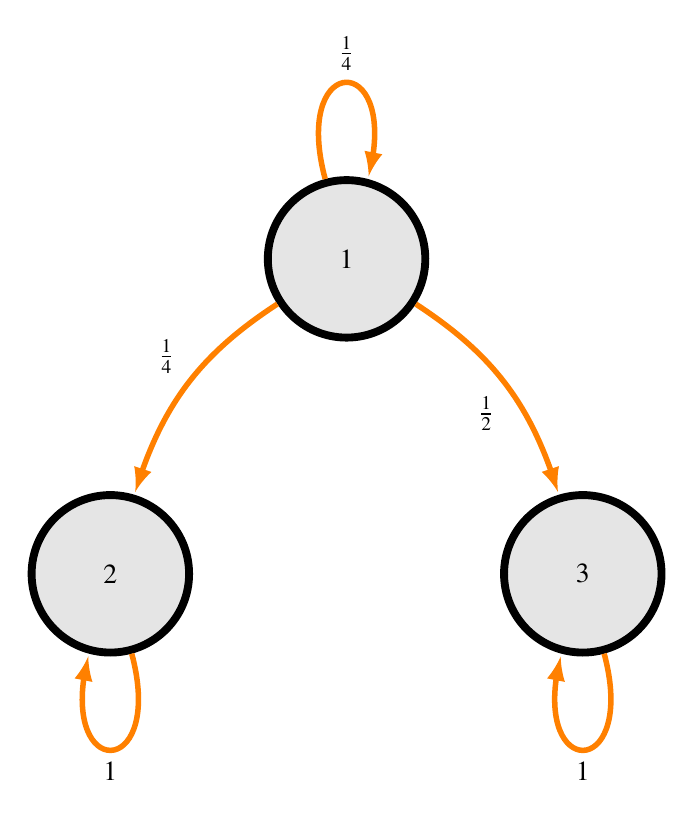
\begin{tikzpicture}
         
               % Setup the style for the states
          \tikzset{node style/.style={state, 
                                      minimum width=2cm,
                                      line width=1mm,
                                      fill=gray!20!white}}
          % Draw the states
          \node[node style] at (3, 0)      (bull)     {1};
          \node[node style] at (0, -4)      (bear)     {2};
          \node[node style] at (6, -4) (stagnant) {3};
          % Connect the states with arrows
          \draw[every loop,
                auto=right,
                line width=0.7mm,
                >=latex,
                draw=orange,
                fill=orange]
             (bull)     edge[bend left=20]            node {$\frac{1}{2}$} (stagnant)
              (bull)     edge[bend right=20] node {$\frac{1}{4}$} (bear)
              
              
              (bull) edge[loop above]             node  {$\frac{1}{4}$} (bull)
              (bear) edge[loop below]             node  {1} (bear)
              (stagnant) edge[loop below]             node  {1} (stagnant);
      \end{tikzpicture}
      \caption{}
      \label{fig:markov/1}
  \end{figure}
  The given problem can be represented using Table \ref{ec9:table:1} and the Markov chain in Fig. \ref{fig:markov/1}.
% Given, a fair coin is tossed is tossed two times.
% Let's define a Markov chain $\{X_{n},n=0,1,2,\dots\}$, where $X_{n}\in S=\{1,2,3\}$, such that
\begin{table}[ht!]
\centering
\begin{tabular}{|c|c|}
    \hline
    State & Description \\
    \hline
    1 & $\cbrak{T, T}$\\[1ex]
    \hline
    2 &  $Y = \cbrak{T, H}$\\[1ex]
    \hline
    3 & $N = \cbrak{\cbrak{H, H},\cbrak{H, T}}$\\[1ex]
    \hline
\end{tabular}
\caption{States and their notations}
\label{ec9:table:1}
\end{table}
The state transition matrix for the Markov chain can be expressed as
\begin{align}
  P=\begin{blockarray}{cccccc}
  &2 & 3 & 1  \\
  \begin{block}{c[ccccc]}
    2 & 1 & 0 & 0  \\
    3 & 0 & 1 & 0 \\
    1 & 0.25 & 0.5 & 0.25  \\
  \end{block}
  \end{blockarray}
  \label{ec9:eq:1}
  \end{align}
%  
Clearly, the state $1$ is transient, while $2,3$ are absorbing. Comparing   \eqref{ec9:eq:1} with the standard form of 
the state transition matrix 
\begin{align}
\label{ec9:eq:2}
P=\begin{blockarray}{ccc}
&A & N \\
\begin{block}{c[cc]}
  A & I & O  \\
  N & R & Q \\
\end{block}
\end{blockarray}
\end{align}
where,
\begin{table}[ht!]
\centering
\caption{Notations and their meanings}
\label{ec9:table:2}
\begin{tabular}{|c|c|}
    \hline
    Notation & Meaning \\
    \hline
    $A$ & All absorbing states\\[1ex]
    \hline
    $N$ & All non-absorbing states\\[1ex]
    \hline
    $I$ & Identity matrix\\[1ex]
    \hline
    $O$ & Zero matrix\\[1ex]
    \hline
    $R,Q$ & Other submatices\\[1ex]
    \hline
\end{tabular}
\end{table}
From   \eqref{ec9:eq:1} and  \eqref{ec9:eq:2},
\begin{align}
\label{ec9:eq:r,q}
    R=\myvec{
    0.25 & 0.5\\
    },
    Q=\myvec{
    0.25\\
    }
\end{align}
The limiting matrix for absorbing Markov chain is
\begin{align}
\bar P=\myvec{
    I & O\\
    FR & O\\
    }
    \label{eq:markov/1/limit}
\end{align}
where
\begin{align}
F=\brak{I-Q}^{-1} = \brak{1-0.25}^{-1} = \frac{4}{3}
\label{eq:markov/1/fund}
\end{align}
is called the fundamental matrix of $P$. 
Upon substituting from \eqref{ec9:eq:r,q} in \eqref{eq:markov/1/fund},
\begin{align}
  F=\brak{1-0.25}^{-1} = \frac{4}{3}
  \end{align}
  %
  and
  \begin{align}
    FR=\myvec{\frac{1}{3} & \frac{2}{3}}
    \end{align}
  which, upon substituting in \eqref{eq:markov/1/limit} yields
\begin{align}
\bar P=\begin{blockarray}{cccccc}
&2 & 3 & 1 \\
\begin{block}{c[ccccc]}
    2 & 1 & 0 & 0\\ 
    3 & 0 & 1 & 0\\ 
    1 & \frac{1}{3} & \frac{2}{3} & 0\\    
\end{block}
\end{blockarray}
\end{align}
% The desired probability is given by $\bar{p}_{12}$
% A element $\bar p_{ij}$ of $\bar P$ denotes the absorption probability in state $j$, starting from state $i$. 

% \\ Then, the absorption probability in state 2 $\brak{\text{i.e getting output Y}}$ starting from state 1 is $\bar p_{12}$.
\begin{align}
\therefore \bar p_{12}=\frac{1}{3}
\end{align}

%
\item Consider a simple symmetric random walk on integers ,Where from every state i you to move to i-1 and i+1 with  probability half each. Then which of the following are correct?
\begin{enumerate}
    \item The random walk is aperiodic
    \item The random walk is irreducible
    \item The random walk is null recurrent 
    \item The random walk is positive recurrent 
\end{enumerate}
%
\solution
This is a Markov Chain ,Where the state space consists of the integers $(i=0,\pm1,\pm2,\pm3,...)$ and transition  probability is given as
\begin{align}
   P_{i,i+1} &= p =\frac{1}{2}
   \\
   P_{i,i-1} & =q =\frac{1}{2}
\end{align}
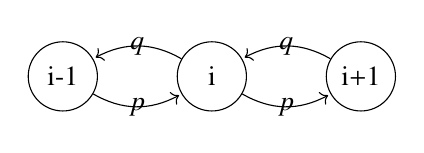
\begin{tikzpicture}
    
    \node[state]  (p) {i-1};
    \node[state,right=of p]  (q) {i};
    \node[state,right=of q]  (r) {i+1};
    \draw[every loop]
    (p) edge[bend right] node {$p $} (q)
    (q) edge[bend right] node {$q $} (p)
    (q) edge[bend right] node {$p$} (r)
    (r) edge[bend right] node {$q $} (q);
   
\end{tikzpicture}
Let $P_{i,j}^{n}$ denotes the probability of being in state j after nth transition starting from state i.
\begin{enumerate}
    \item We know that for state j in Markov chain to be \textbf{aperiodic} ,Then their  exist k such that $P_{j,j}^{n} > 0$ for all $n \geq k$. but for to return to same state j after n transitions  ,Number of forward steps should be equal to Backward steps , i.e for odd n in (2m +1)form
    \begin{align}
        P_{j,j}^{2m+1}&=0  
        \label{2019/105/eq:eq1}
    \end{align}
    when n is even in 2m form
    \begin{align}
        P_{j,j}^{2m}&=\binom{2m}{m}p^{m}q^{m}
     \\
     &=\frac{(2m)!}{m!.m!}p^{m}q^{m}
     \label{2019/105/eq:eq2}
    \end{align}
    ,As for odd n $P_{j,j}^{n} = 0$ ,$P_{j,j}^{n} > 0$ for all $n \geq k$ is not possible .which implies  all states are \textbf{Periodic}
  
    Option (1) is \textbf{incorrect}. 
    \item 
In a Markov Chain for state j to be recurrent then it should satisfy following condition
\begin{align}
     \lim_{t\to\infty}\sum_{n=1}^t P_{j,j}^{n}&=\infty
\end{align}
using Stirling approximation in equation \eqref{2019/105/eq:eq2} 
\begin{align}
    P_{j,j}^{2m} &=\frac{((2m)^{2m +\frac{1}{2}}).e^{-2m}.(2\pi)^{\frac{1}{2}}}{m^{m+\frac{1}{2}}.e^{-m}.m^{m+\frac{1}{2}}.e^{-m}.2\pi}.p^{m}q^{m}
    \\
    &=\frac{(4pq)^{2m}}{(m\pi)^{\frac{1}{2}}}
    \label{2019/105/eq:eq3}
\end{align}
In this question $p =\frac{1}{2}=q$,then using \eqref{2019/105/eq:eq1} and \eqref{2019/105/eq:eq3}
\begin{align}
    \lim_{t\to\infty}\sum_{n=1}^t P_{j,j}^{n}&=\sum_{n=2k,k=1}^{\infty}\frac{1}{(\frac{n}{2}\pi)^{\frac{1}{2}}}
\end{align}
Since $\frac{1}{n^{\frac{1}{2}}}$ is divergent,
\begin{align}
     \lim_{t\to\infty}\sum_{n=1}^t P_{j,j}^{n}& = \infty
\end{align}
Therefore state j is recurrent ,as what we calculated is independent of j ,all states are \textbf{recurrent }.
The first-passage-time probability, $f_{i,j}(n)$, of a Markov chain is the probability,given as 
\begin{equation}
\resizebox{.9\hsize}{!}{$f_{i,j}(n)=\pr{X_{n}=j,X_{n-1}\neq j,X_{n-2}\neq j,\dots X_{1}\neq j|X_{0}=i}$}
\end{equation}
The first-passage time $T_{j,j}$from a state j back to itself is of particular importance. It has the PMF $f_{j,j}(n)$ amd Distribution function $F_{j,j}(n)$
\begin{align}
    F_{j,j}(n)&=\sum_{k=0}^n f_{j,j}(k)
    \label{2019/105/eq:eq4}
\end{align}
We Know that all states are recurrent .Now i will find whether they are null recurrent or positive recurrent .
For positive recurrent 
\begin{align}
    \overline{T_{j,j}}& < \infty
\end{align}
For null recurrent 
\begin{align}
    \overline{T_{j,j}}& = \infty
\end{align}
Where $\overline{T_{j,j}}$ is mean time to enter state j starting from j.
Now calculating $\overline{T_{j,j}}$ using below formula,
\begin{align}
    \overline{T_{j,j}}&=1 + \sum _{k=0}^n (1 - F_{j,j}(k))
    \label{2019/105/eq:eq5}
\end{align}
Using \eqref{2019/105/eq:eq5} and \eqref{2019/105/eq:eq4},We get 
\begin{align}
    \overline{T_{j,j}}& = \infty
\end{align}
Therefore all states are null recurrent.
Option(3) is \textbf{correct}
 \item
    Since all states are recurrent,they communicate with each other ,therefore Markov chain is irreducible , option (2) is \textbf{correct}
 \item As all states are null recurrent , option (4) is \textbf{incorrect} 
\end{enumerate}
Therefore correct options are \textbf{2,3}




\item Consider a Markov Chain with state space $\cbrak{0,1,2}$ and transition matrix
\begin{align}
P = 
\begin{blockarray}{c@{\hspace{1pt}}rrr@{\hspace{3pt}}}
         & 0   & 1   & 2 \\
        \begin{block}{r@{\hspace{3pt}}@{\hspace{1pt}}
    (@{\hspace{1pt}}rrr@{\hspace{1pt}}@{\hspace{1pt}})}
        0 & \frac{1}{4} & \frac{5}{8} & \frac{1}{8}  \\[1mm]
        1 & \frac{1}{4} & 0 & \frac{3}{4}  \\[1mm]
        2 &  \frac{1}{2} & \frac{3}{8} & \frac{1}{8}  \\
        \end{block}
    \end{blockarray}
\end{align}
Then which of the following are true?
\begin{enumerate}
\item $\lim_{n \to \infty} p_{12}^{(n)} = 0$
\item $\lim_{n \to \infty} p_{12}^{(n)} = \lim_{n \to \infty} p_{21}^{(n)}$
\item $\lim_{n \to \infty} p_{22}^{(n)} = \frac{1}{8}$
\item $\lim_{n \to \infty} p_{21}^{(n)} = \frac{1}{3}$
\end{enumerate}

%
\item Consider a Markov chain with state space {1,2,....,100}. Suppose states 2i and 2j communicate with each other and states 2i-1 and 2j-1 communicate with each other for every i,j = 1,2,...,50. Further suppose that $p^{(2)}_{3,3}$ > 0,$p^{(3)}_{4,4}$ > 0 and $p^{(7)}_{2,5}$ > 0. Then 
\begin{enumerate}
\item The Markov chain is irreducible.
\item The Markov chain is aperiodic.
\item State 8 is recurrent.
\item State 9 is recurrent.
\end{enumerate}
%
\solution
\input{solutions/2014/dec/106/LaTex/Assignment_7.tex}
%
%
\item A standard fair die is rolled until some face other than 5 or 6 turns up.Let X denote the face value of the last roll.Let A=\{X is even\} and B=\{X is atmost 2\}
Then,
\begin{enumerate}
\begin{multicols}{2}
\setlength\itemsep{1em}
\item $\Pr{(A\cap {B})}=0$\\
\item $\Pr{(A \cap B)}=\frac{1}{6}$\\
\item $\Pr{(A\cap B)}=\frac{1}{4}$\\
\item $\Pr{({A} \cap {B})}=\frac{1}{3}$
\end{multicols}
\end{enumerate}
%
\solution
\begin{figure}[h!]
    \caption{Markov chain}
    \resizebox{\columnwidth}{!}{%
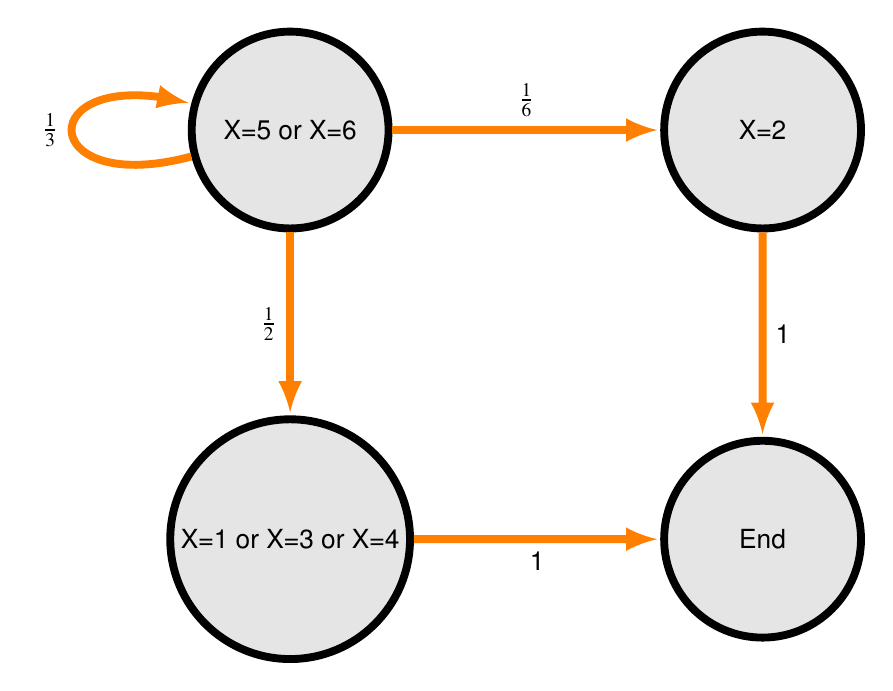
\begin{tikzpicture}[font=\sffamily]
        % Setup the style for the states
        \tikzset{node style/.style={state, 
                                    minimum width=2.5cm,
                                    line width=1mm,
                                    fill=gray!20!white}}
        % Draw the states
        \node[node style] at (0, 0)     (A)     {X=5 or X=6};
        \node[node style] at (6, 0)     (B)     {X=2};
        \node[node style] at (6, -5.196) (end) {End};
        \node[node style] at (0, -5.196) (C) {X=1 or X=3 or X=4};
        % Connect the states with arrows
        \draw[every loop,
              auto=right,
              line width=1mm,
              >=latex,
              draw=orange,
              fill=orange]
              (A) edge[bend left=0] node {$\frac{1}{2}$} (C)
              (C) edge[bend left=0] node {1} (end)
              (A) edge[loop left] node {$\frac{1}{3}$} (A)
            (A)     edge[bend right=0, auto=left] node {$\frac{1}{6}$} (B)
            (B)     edge[bend left=0, auto=left] node {1} (end);
    \end{tikzpicture}
    }
    \end{figure}
Let us assume the following table.
\begin{table}[h!]
\centering
\caption{}
\label{june2018-49:table:1}
\resizebox{\columnwidth}{!}{%
\begin{tabular}{|c|c|c|c|}
    \hline
    state 1&state 2 &state 3 &state 4\\
    \hline
$X=5$ or $X=6$&$X=2$&$X=1$ or $X=3$ or $X=4$ &end \\    
    \hline
\end{tabular}}
\end{table}
Let us represent the markov chain diagram in a matrix.Let $P_{ij}$ represent the element of a matrix which is in $i^{th}$ row and $j^{th}$ column.The value of $P_{ij}$ is equal to probability of transition from state $i$ to state $j$
\begin{equation}
P=\begin{bmatrix}
\frac{1}{3}&\frac{1}{6}&\frac{1}{2}&0\\
0&0&0&1\\
0&0&0&1\\
0&0&0&0\\
\end{bmatrix}
\end{equation}
We need the probability that $X=2$.Hence required probability is
\begin{equation}
    P_{12}+(P_{12})^{2}+\cdots+\infty \label{june2018-49:eq:reqprob}
\end{equation}
where $P_{12}^{n}$ represents the 1st row ,2nd column element in the $P^{n}$
\begin{align}
P^2&=\begin{bmatrix}
\frac{1}{3}&\frac{1}{6}&\frac{1}{2}&0\\
0&0&0&1\\
0&0&0&1\\
0&0&0&0\\
\end{bmatrix} \times
\begin{bmatrix}
\frac{1}{3}&\frac{1}{6}&\frac{1}{2}&0\\
0&0&0&1\\
0&0&0&1\\
0&0&0&0\\
\end{bmatrix}\\
&=\begin{bmatrix}
\frac{1}{9}&\frac{1}{18}&\frac{1}{6}&0\\
0&0&0&0\\
0&0&0&0\\
0&0&0&0\\
\end{bmatrix}
\end{align}
\begin{align}
    P^3&=(P^2)(P^1)\\
    &=\begin{bmatrix}
\frac{1}{9}&\frac{1}{18}&\frac{1}{6}&0\\
0&0&0&0\\
0&0&0&0\\
0&0&0&0\\
\end{bmatrix}\times
\begin{bmatrix}
\frac{1}{3}&\frac{1}{6}&\frac{1}{2}&0\\
0&0&0&1\\
0&0&0&1\\
0&0&0&0\\
\end{bmatrix}\\
&=\begin{bmatrix}
\frac{1}{27}&\frac{1}{54}&\frac{1}{18}&0\\
0&0&0&0\\
0&0&0&0\\
0&0&0&0\\
\end{bmatrix}
\end{align}
From above we can notice that each time $P_{12}$ reduces by $\frac{1}{3}$.Hence from \eqref{june2018-49:eq:reqprob},
\begin{equation}
    \sum_{i=0}^{\infty}\brak{\frac{1}{3}}^i \frac{1}{6}
\end{equation}
From Geometric progression we can write ,required probability =$\frac{1}{4}$
$\therefore$ \textbf{option C is correct}
\item %
Consider a Markov chain with five states $\{1,2,3,4,5\}$ and transition matrix
\begin{align}
    P=\myvec{\frac{1}{2} & 0 & 0 & \frac{1}{2} & 0\\
            0 & \frac{1}{7} & 0 & 0&\frac{6}{7}\\
              \frac{1}{5} & \frac{1}{5} & \frac{1}{5} & \frac{1}{5} & \frac{1}{5}\\ \frac{1}{3} & 0 & 0 & \frac{2}{3} & 0 \\
              0 & \frac{5}{8} & 0 & 0 & \frac{3}{8}}
\end{align}
Which of the following are true?
\begin{enumerate}
\item 3 and 1 are in the same communicating class
\item 1 and 4 are in the same communicating class
\item 4 and 2 are in the same communicating class
\item 2 and 5 are in the same communicating class
\end{enumerate}
%
\solution
See Tables \ref{eq:solutions/2017/dec/105/table0} and \ref{eq:solutions/2017/dec/105/table1}

\begin{table*}[!ht]
\centering
\resizebox{2\columnwidth}{!}
{
\begin{tabular}{|l|l|}
	\hline
	\multirow{3}{*}{Accessibility of states} 
	& \\
	& We say that state $j$ is accessible from state $i$, written as $i \rightarrow j$, if $p^{(n)}_{ij}>0$\\ in Markov's chain
	& for some n. Every state is accessible from itself since $p^{(0)}_{ii}=1$\\
	&\\
	\hline
	\multirow{3}{*}{Communication between} & \\
	& Two states $i$ and $j$ are said to communicate, written as $i\leftrightarrow j$, if they\\ states
	& are accessible from each other. In other words,\\
	&\\
  	& \qquad \qquad  \qquad $i \leftrightarrow j  \;  \textrm{ means } \;  i \rightarrow j  \textrm{ and }  j \rightarrow i.$ \\
    	& \\
    	\hline
    	\multirow{3}{*}{Communicating class} & \\
	& For each Markov chain, there exists a unique decomposition of the \\
	& state space $S$ into a sequence of disjoint subsets $C_1, C_2, . . .,$\\
	&\\
    	&  \qquad \qquad  \qquad$S=\bigcup_{i=1}^{\infty}C_i$\\
    	&\\
    	& in which each subset has the property that all states within it communicate.\\
    	& Each such subset is called a communication class of the Markov chain.\\
    	&\\
    \hline
\end{tabular}
}
\caption{Definition and Result used}
\label{eq:solutions/2017/dec/105/table0}
\end{table*}
%\usepackage{longtable}
%\begin{table*}
%\centering
\onecolumn
	\begin{longtable}{|l|l|}
		\hline
		\multirow{3}{*}{Drawing Transition diagram} 
		& \\
		& 
		
		
\tikzset{every picture/.style={line width=0.75pt}} %set default line width to 0.75pt        
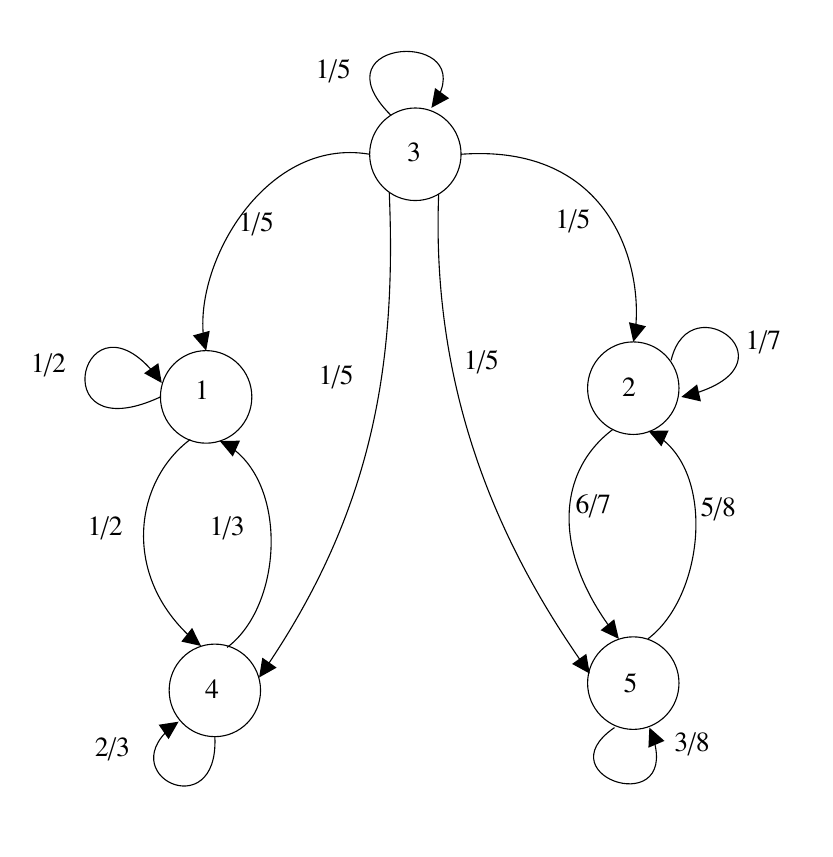
\begin{tikzpicture}[x=0.75pt,y=0.75pt,yscale=-0.7,xscale=0.7]
%uncomment if require: \path (0,714); %set diagram left start at 0, and has height of 714
%Shape: Ellipse [id:dp29836895541013164] 
\draw   (286,156.85) .. controls (286,139.26) and (300.08,125) .. (317.45,125) .. controls (334.82,125) and (348.9,139.26) .. (348.9,156.85) .. controls (348.9,174.44) and (334.82,188.7) .. (317.45,188.7) .. controls (300.08,188.7) and (286,174.44) .. (286,156.85) -- cycle ;
%Shape: Ellipse [id:dp4858180433459096] 
\draw   (142,323.85) .. controls (142,306.26) and (156.08,292) .. (173.45,292) .. controls (190.82,292) and (204.9,306.26) .. (204.9,323.85) .. controls (204.9,341.44) and (190.82,355.7) .. (173.45,355.7) .. controls (156.08,355.7) and (142,341.44) .. (142,323.85) -- cycle ;
%Shape: Ellipse [id:dp10893001214881792] 
\draw   (436,317.85) .. controls (436,300.26) and (450.08,286) .. (467.45,286) .. controls (484.82,286) and (498.9,300.26) .. (498.9,317.85) .. controls (498.9,335.44) and (484.82,349.7) .. (467.45,349.7) .. controls (450.08,349.7) and (436,335.44) .. (436,317.85) -- cycle ;
%Shape: Ellipse [id:dp31584444241771226] 
\draw   (148,525.85) .. controls (148,508.26) and (162.08,494) .. (179.45,494) .. controls (196.82,494) and (210.9,508.26) .. (210.9,525.85) .. controls (210.9,543.44) and (196.82,557.7) .. (179.45,557.7) .. controls (162.08,557.7) and (148,543.44) .. (148,525.85) -- cycle ;
%Shape: Ellipse [id:dp6845584977543557] 
\draw   (436,520.85) .. controls (436,503.26) and (450.08,489) .. (467.45,489) .. controls (484.82,489) and (498.9,503.26) .. (498.9,520.85) .. controls (498.9,538.44) and (484.82,552.7) .. (467.45,552.7) .. controls (450.08,552.7) and (436,538.44) .. (436,520.85) -- cycle ;
%Curve Lines [id:da40673715992947246] 
\draw    (212.24,513.63) .. controls (288.82,402.26) and (304.45,300.14) .. (299.5,183.32) ;
\draw [shift={(209.9,517)}, rotate = 304.9] [fill={rgb, 255:red, 0; green, 0; blue, 0 }  ][line width=0.08]  [draw opacity=0] (12.5,-6.01) -- (0,0) -- (12.5,6.01) -- cycle    ;
%Curve Lines [id:da5133467038577342] 
\draw    (172.69,288.89) .. controls (161.52,237.16) and (212.5,144.11) .. (286,156.85) ;
\draw [shift={(173.45,292)}, rotate = 254.65] [fill={rgb, 255:red, 0; green, 0; blue, 0 }  ][line width=0.08]  [draw opacity=0] (12.5,-6.01) -- (0,0) -- (12.5,6.01) -- cycle    ;
%Curve Lines [id:da008345831811055193] 
\draw    (167.44,493.28) .. controls (114.6,449.49) and (123.1,382.7) .. (162.5,353.15) ;
\draw [shift={(169.9,495.27)}, rotate = 218.21] [fill={rgb, 255:red, 0; green, 0; blue, 0 }  ][line width=0.08]  [draw opacity=0] (12.5,-6.01) -- (0,0) -- (12.5,6.01) -- cycle    ;
%Curve Lines [id:da5634268603548509] 
\draw    (435.25,511.14) .. controls (385.72,441.07) and (327.59,334.04) .. (333.5,184.32) ;
\draw [shift={(437.5,514.32)}, rotate = 234.46] [fill={rgb, 255:red, 0; green, 0; blue, 0 }  ][line width=0.08]  [draw opacity=0] (12.5,-6.01) -- (0,0) -- (12.5,6.01) -- cycle    ;
%Curve Lines [id:da4259073730032066] 
\draw    (187.9,496.27) .. controls (227.3,466.72) and (230.27,378.53) .. (185,355.28) ;
\draw [shift={(182.9,354.27)}, rotate = 384.44] [fill={rgb, 255:red, 0; green, 0; blue, 0 }  ][line width=0.08]  [draw opacity=0] (12.5,-6.01) -- (0,0) -- (12.5,6.01) -- cycle    ;
%Curve Lines [id:da6577514807411684] 
\draw    (468.08,283.01) .. controls (475.64,242.78) and (457.71,148.87) .. (348.9,156.85) ;
\draw [shift={(467.45,286)}, rotate = 283.29] [fill={rgb, 255:red, 0; green, 0; blue, 0 }  ][line width=0.08]  [draw opacity=0] (12.5,-6.01) -- (0,0) -- (12.5,6.01) -- cycle    ;
%Curve Lines [id:da329541870026538] 
\draw    (142,323.85) .. controls (58.35,362.99) and (88.88,241.85) .. (141.3,312.08) ;
\draw [shift={(142.9,314.27)}, rotate = 234.51] [fill={rgb, 255:red, 0; green, 0; blue, 0 }  ][line width=0.08]  [draw opacity=0] (12.5,-6.01) -- (0,0) -- (12.5,6.01) -- cycle    ;
%Curve Lines [id:da3393212160499588] 
\draw    (493.5,298.66) .. controls (506.37,243.94) and (584.91,303.18) .. (503.03,323.29) ;
\draw [shift={(500.5,323.88)}, rotate = 347.23] [fill={rgb, 255:red, 0; green, 0; blue, 0 }  ][line width=0.08]  [draw opacity=0] (12.5,-6.01) -- (0,0) -- (12.5,6.01) -- cycle    ;
%Curve Lines [id:da7968400462935867] 
\draw    (477.5,490.39) .. controls (516.9,460.84) and (525.1,371.56) .. (480,348.28) ;
\draw [shift={(477.9,347.27)}, rotate = 384.44] [fill={rgb, 255:red, 0; green, 0; blue, 0 }  ][line width=0.08]  [draw opacity=0] (12.5,-6.01) -- (0,0) -- (12.5,6.01) -- cycle    ;
%Curve Lines [id:da49532662514959913] 
\draw    (455.47,487.82) .. controls (411.57,431.68) and (414.1,375.7) .. (453.5,346.15) ;
\draw [shift={(457.5,490.39)}, rotate = 231.1] [fill={rgb, 255:red, 0; green, 0; blue, 0 }  ][line width=0.08]  [draw opacity=0] (12.5,-6.01) -- (0,0) -- (12.5,6.01) -- cycle    ;
%Curve Lines [id:da618838807270425] 
\draw    (179.45,557.7) .. controls (182.46,620.43) and (105.86,583.53) .. (152.3,548.96) ;
\draw [shift={(154.5,547.39)}, rotate = 505.54] [fill={rgb, 255:red, 0; green, 0; blue, 0 }  ][line width=0.08]  [draw opacity=0] (12.5,-6.01) -- (0,0) -- (12.5,6.01) -- cycle    ;
%Curve Lines [id:da7726575310463464] 
\draw    (479.68,554.36) .. controls (503.45,616.53) and (404.27,585.93) .. (454.51,551.46) ;
\draw [shift={(478.51,551.46)}, rotate = 67.01] [fill={rgb, 255:red, 0; green, 0; blue, 0 }  ][line width=0.08]  [draw opacity=0] (12.5,-6.01) -- (0,0) -- (12.5,6.01) -- cycle    ;
%Curve Lines [id:da7210031613710599] 
\draw    (330.71,121.65) .. controls (363.66,70.1) and (246.61,75.98) .. (300.51,129.88) ;
\draw [shift={(328.51,124.88)}, rotate = 306.03] [fill={rgb, 255:red, 0; green, 0; blue, 0 }  ][line width=0.08]  [draw opacity=0] (12.5,-6.01) -- (0,0) -- (12.5,6.01) -- cycle    ;
% Text Node
\draw (164,311.21) node [anchor=north west][inner sep=0.75pt]   [align=left] {{\normalsize 1}};
% Text Node
\draw (458,309.21) node [anchor=north west][inner sep=0.75pt]   [align=left] {{\normalsize 2}};
% Text Node
\draw (171,517.21) node [anchor=north west][inner sep=0.75pt]   [align=left] {{\normalsize 4}};
% Text Node
\draw (459,512.21) node [anchor=north west][inner sep=0.75pt]   [align=left] {{\normalsize 5}};
% Text Node
\draw (310,147.21) node [anchor=north west][inner sep=0.75pt]   [align=left] {{\normalsize 3}};
% Text Node
\draw (51,292.21) node [anchor=north west][inner sep=0.75pt]   [align=left] {{\normalsize 1/2}};
% Text Node
\draw (90,404.21) node [anchor=north west][inner sep=0.75pt]   [align=left] {{\normalsize 1/2}};
% Text Node
\draw (543,276.21) node [anchor=north west][inner sep=0.75pt]   [align=left] {{\normalsize 1/7}};
% Text Node
\draw (174,404.21) node [anchor=north west][inner sep=0.75pt]   [align=left] {{\normalsize 1/3}};
% Text Node
\draw (194,195.21) node [anchor=north west][inner sep=0.75pt]   [align=left] {{\normalsize 1/5}};
% Text Node
\draw (426,389.21) node [anchor=north west][inner sep=0.75pt]   [align=left] {{\normalsize 6/7}};
% Text Node
\draw (512,391.21) node [anchor=north west][inner sep=0.75pt]   [align=left] {{\normalsize 5/8}};
% Text Node
\draw (95,556.21) node [anchor=north west][inner sep=0.75pt]   [align=left] {{\normalsize 2/3}};
% Text Node
\draw (494,553.21) node [anchor=north west][inner sep=0.75pt]   [align=left] {{\normalsize 3/8}};
% Text Node
\draw (247,90.21) node [anchor=north west][inner sep=0.75pt]   [align=left] {{\normalsize 1/5}};
% Text Node
\draw (249,300.21) node [anchor=north west][inner sep=0.75pt]   [align=left] {{\normalsize 1/5}};
% Text Node
\draw (349,290.21) node [anchor=north west][inner sep=0.75pt]   [align=left] {{\normalsize 1/5}};
% Text Node
\draw (412,193.21) node [anchor=north west][inner sep=0.75pt]   [align=left] {{\normalsize 1/5}};
\end{tikzpicture}

		
		
		\\  
		&\\
		&\\
		\hline
		\multirow{3}{*}{Checking whether the  } & \\
		& Here,\\states 3 and 1 are in the
		& State 1 is accessible from the state 3.\\same communicating class
	    	& But, State 3 is not accessible from the state 1\\
	    	& \qquad \qquad \qquad i.e.  $3 \rightarrow 1$,  $1 \nrightarrow 3$\\
	    	& \qquad \qquad \qquad$\implies \boxed{3 \nleftrightarrow 1}$\\
	    	&\\ 
	    	&Therefore, 3 and 1 are not in the same communicating class.\\
	   	&\\
	   	\hline
	   \multirow{3}{*}{Checking whether the  } & \\
		& Here,\\states 1 and 4 are in the
		& State 1 is accessible from the state 4.\\same communicating class
	    	& Also, State 4 is accessible from the state 1\\
	    	& \qquad \qquad \qquad i.e.  $3 \rightarrow 1$,  $1 \rightarrow 3$\\
	   	& \qquad \qquad \qquad$\implies \boxed{3 \leftrightarrow 1}$\\
	    	&\\ 
	    	&Therefore, 1 and 4 are in the same communicating class.\\	   	
	   	&\\	   	
	   	\hline
	   	\multirow{3}{*}{Checking whether the  } & \\
		& Here,\\states 4 and 2 are in the
		& State 2 is not accessible from the state 4.\\same communicating class
	    	& Also, State 4 is not accessible from the state 2\\
	    	& \qquad \qquad \qquad i.e.  $4 \nrightarrow 2$,  $2 \nrightarrow 4$\\
	    	\hline
	    	&\\	    	
	   	& \qquad \qquad \qquad$\implies \boxed{4 \nleftrightarrow 2}$\\
	    	&Therefore, 4 and 2 are not in the same communicating class.\\
	   	&\\
	   	\hline
	   	\multirow{3}{*}{Checking whether the  } & \\
		& Here,\\states 2 and 5 are in the
		& State 2 is accessible from the state 5.\\same communicating class
	    	& Also, State 5 is accessible from the state 2\\
	    	& \qquad \qquad \qquad i.e.  $5 \rightarrow 2$,  $2 \rightarrow 5$\\
	   	& \qquad \qquad \qquad$\implies \boxed{2 \leftrightarrow 5}$\\
	    	&\\
	    	&Therefore, 2 and 5 are in the same communicating class.\\
	   	&\\
	   	\hline
	   	\multirow{3}{*}{Conclusion} & \\
	   	&Communication classes are:\\
	   	&\\
	   	& \qquad \qquad \qquad$\boxed{S=\{1,4\}\cup \{3\} \cup \{2,5\}}$\\
	   	&\\
		&Option 2) and 4) are true.\\
	   	&\\
	   	\hline
\caption{Solution}
\label{eq:solutions/2017/dec/105/table1}
    \end{longtable}
%\end{table*}
\twocolumn


%\twocolumn 
%
\item $A$ and $B$ play a game of tossing a fair coin. $A$ starts the game by tossing the coin once and $B$ then tosses the coin twice, followed by $A$ tossing the coin once and $B$ tossing the coin twice and this continues until a head turns up. Whoever gets the first head wins the game. Then, 
\begin{enumerate}
    \item $P(B$ Wins) $> P(A$ Wins)
    \item $P(B$ Wins) $= 2P(A$ Wins)
    \item $P(A$ Wins) $> P(B$ Wins)
    \item $P(A$ Wins) $= 1-P(B$ Wins)
\end{enumerate}
%
%
\solution
Given, a fair coin is tossed till heads turns up.
\begin{align}
\tag{104.1}
\label{dec2016-104eq:0}
    p=\dfrac{1}{2},q=\dfrac{1}{2}
\end{align}
Let's define a Markov chain $\{X_{n},n=0,1,2,\dots\}$, where $X_{n}\in S=\{1,2,3,4,5\}$, such that
\begin{table}[h!]
\centering
\caption{States and their notations}
\label{dec2016-104table:1}
\begin{tabular}{|c|c|}
    \hline
    Notation & State \\
    \hline
    $S=1$ & $A$'s turn\\[1ex]
    \hline
    $S=2$ & $B$'s first turn\\[1ex]
    \hline
    $S=3$ & $B$'s second turn\\[1ex]
    \hline
    $S=4$ & $A$ wins\\[1ex]
    \hline
    $S=4$ & $B$ wins\\[1ex]
    \hline
\end{tabular}
\end{table}
The state transition matrix for the Markov chain is
\begin{align}
\tag{104.2}
\label{dec2016-104eq:p}
    P=\begin{blockarray}{cccccc}
&1 & 2 & 3 & 4 & 5 \\
\begin{block}{c[ccccc]}
  1 & 0 & 0.5 & 0 & 0.5 & 0 \\
  2 & 0 & 0 & 0.5 & 0 & 0.5 \\
  3 & 0.5 & 0 & 0 & 0 & 0.5 \\
  4 & 0 & 0 & 0 & 1 & 0 \\
  5 & 0 & 0 & 0 & 0 & 1 \\
\end{block}
\end{blockarray}
\end{align}
Clearly, the states $1,2,3$ are transient, while $4,5$ are absorbing. The standard form of a state transition matrix is
\begin{align}
\tag{104.3}
\label{dec2016-104eq:std}
    P=\begin{blockarray}{ccc}
&A & N \\
\begin{block}{c[cc]}
  A & I & O  \\
  N & R & Q \\
\end{block}
\end{blockarray}
\end{align}
where,
\begin{table}[h!]
\centering
\caption{Notations and their meanings}
\label{dec2016-104table:2}
\begin{tabular}{|c|c|}
    \hline
    Notation & Meaning \\
    \hline
    $A$ & All absorbing states\\[1ex]
    \hline
    $N$ & All non-absorbing states\\[1ex]
    \hline
    $I$ & Identity matrix\\[1ex]
    \hline
    $O$ & Zero matrix\\[1ex]
    \hline
    $R,Q$ & Other submatices\\[1ex]
    \hline
\end{tabular}
\end{table}
Converting \eqref{dec2016-104eq:p} to standard form, we get
\begin{align}
\tag{104.4}
\label{dec2016-104eq:pstd}
    P=\begin{blockarray}{cccccc}
&4 & 5 & 1 & 2 & 3 \\
\begin{block}{c[ccccc]}
  4 & 1 & 0 & 0 & 0 & 0 \\
  5 & 0 & 1 & 0 & 0 & 0 \\
  1 & 0.5 & 0 & 0 & 0.5 & 0 \\
  2 & 0 & 0.5 & 0 & 0 & 0.5 \\
  3 & 0 & 0.5 & 0.5 & 0 & 0 \\
\end{block}
\end{blockarray}
\end{align}
From \eqref{dec2016-104eq:pstd},
\begin{align}
\tag{104.5}
\label{dec2016-104eq:r,q}
    R=\begin{bmatrix}
    0.5 & 0\\
    0 & 0.5\\
    0 & 0.5\\
    \end{bmatrix},
    Q=\begin{bmatrix}
    0 & 0.5 & 0\\
    0 & 0 & 0.5\\
    0.5 & 0 & 0\\
    \end{bmatrix}
\end{align}
\newpage
The limiting matrix for absorbing Markov chain is
\begin{align}
\tag{104.6}
\label{dec2016-104eq:pbar}
    \bar P=\begin{bmatrix}
    I & O\\
    FR & O\\
    \end{bmatrix}
\end{align}
where,
\begin{align}
\tag{104.7}
\label{dec2016-104eq:f}
    F=(I-Q)^{-1}
\end{align}
is called the fundamental matrix of $P$. \\
On solving, we get
\begin{align}
\tag{104.8}
\label{dec2016-104eq:ans}
    \bar P=\begin{blockarray}{cccccc}
&4 & 5 & 1 & 2 & 3 \\
\begin{block}{c[ccccc]}
    4 & 1 & 0 & 0 & 0 & 0 \\
    5 & 0 & 1 & 0 & 0 & 0 \\
    1 & 0.5714 & 0.4285 & 0 & 0 & 0 \\
    2 & 0.1428 & 0.8571 & 0 & 0 & 0 \\
    3 & 0.2857 & 0.7142 & 0 & 0 & 0 \\
   \end{block}
\end{blockarray}
\end{align}
A element $\bar p_{ij}$ of $\bar P$ denotes the absorption probability in state $j$, starting from state $i$. Then,
\begin{enumerate}
    \item $Pr(A$ wins)=$\bar p_{14}\approx0.5714$
    \item $Pr(B$ wins)=$\bar p_{15}\approx0.4285$
\end{enumerate}
\begin{align}
\tag{104.9}
\therefore \bar p_{14} > \bar p_{15}
\end{align}
Also, in $\bar P$, all the terms in every row should sum to 1.
\begin{align}
\tag{104.10}
\Rightarrow \bar p_{14} + \bar p_{15}+ 0+0+0=1\\
\tag{104.11}
\therefore \bar p_{14}=1-\bar p_{15}
\end{align}
Therefore, options $3),4)$ are correct.\\
\begin{figure}[h]
\caption*{\textbf{Markov chain diagram}}
\centering
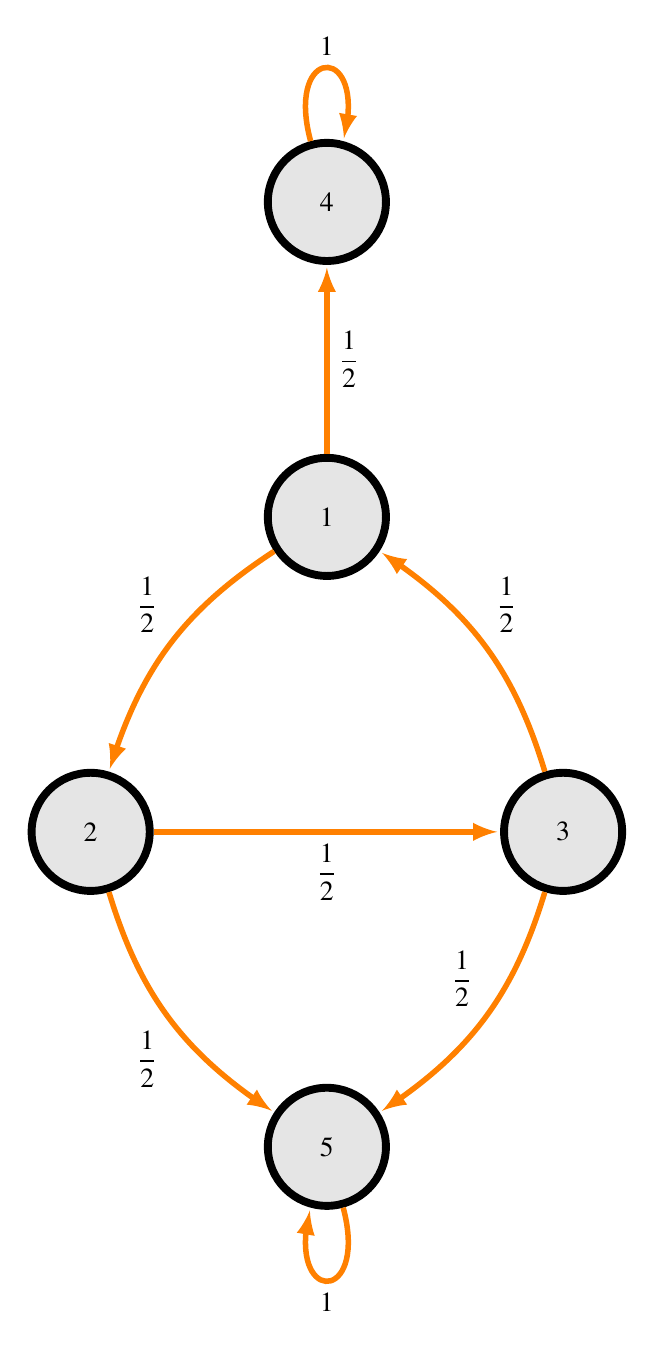
\begin{tikzpicture}
    % Setup the style for the states
        \tikzset{node style/.style={state, 
                                    minimum width=1.5cm,
                                    line width=1mm,
                                    fill=gray!20!white}}
        % Draw the states
        \node[node style] at (3, -4)      (bull)     {1};
        \node[node style] at (0, -8)      (bear)     {2};
        \node[node style] at (6, -8) (stagnant) {3};
        \node[node style] at (3, 0) (over1) {4};
        \node[node style] at (3, -12) (over2) {5};
        % Connect the states with arrows
        \draw[every loop,
              auto=right,
              line width=0.7mm,
              >=latex,
              draw=orange,
              fill=orange]
            (stagnant)     edge[bend right=20]            node {$\dfrac{1}{2}$} (bull)
            (stagnant)     edge[bend left=20]            node {$\dfrac{1}{2}$} (over2)
            (bull)     edge[bend right=20] node {$\dfrac{1}{2}$} (bear)
            (bull)     edge node {$\dfrac{1}{2}$} (over1)
            (bear)     edge[bend right=20] node {$\dfrac{1}{2}$} (over2)
            (bear)     edge node {$\dfrac{1}{2}$} (stagnant)
            (over1) edge[loop above]             node  {1} (over1)
            (over2) edge[loop below]             node  {1} (over2);
\end{tikzpicture}
\end{figure}
\item Consider a Markov chain with state space {1,2,....,100}. Suppose states 2i and 2j communicate with each other and states 2i-1 and 2j-1 communicate with each other for every i,j = 1,2,...,50. Further suppose that $p^{(2)}_{3,3}$ > 0,$p^{(3)}_{4,4}$ > 0 and $p^{(7)}_{2,5}$ > 0. Then 
\begin{enumerate}
\item The Markov chain is irreducible.
\item The Markov chain is aperiodic.
\item State 8 is recurrent.
\item State 9 is recurrent.
\end{enumerate}
\solution
\input{solutions/2014/dec/106/LaTex/Assignment_7.tex}


\end{enumerate}

%
%
\section{Inequalities}
\renewcommand{\theequation}{\theenumi}
\renewcommand{\thefigure}{\theenumi}
\renewcommand{\thetable}{\theenumi}
\begin{enumerate}[label=\thesection.\arabic*.,ref=\thesection.\theenumi]
\numberwithin{equation}{enumi}
\numberwithin{figure}{enumi}
\numberwithin{table}{enumi}


%
\item Let $X_i 's$ be independent random variables such that $X_i 's$ are symmetric about 0 and $var(X_i)=2i - 1$,for $i\geq 1$.then,
$\lim_{n \to \infty}\pr{X_1 +X_2 + \dots + X_n > n\log{n}}$
\begin{enumerate}
\begin{multicols}{2}
\setlength\itemsep{2em}
\item does not exist.
\item equals $\dfrac{1}{2}$.\\
\item equals 1.
\item equals 0.
\end{multicols}
\end{enumerate}
%
\solution
Let $X= X_1 +X_2 + \dots + X_n $,
as $X_i 's$ are symmetric about 0.
The mean of X is given by,
\begin{align}
E[X]=0 \label{dec2015-53:a}
\end{align}
the variance of X is given by,
\begin{align}
var[X]&= \sum_{i=1}^{n}(2i -1)\\
   &= \frac{2n(n+1)}{2} - n\\
   &= n^{2}
\end{align}
the standard deviation,
\begin{align}
\sigma_X = n \label{dec2015-53:b}
\end{align}
Applying Chebyshev's Inequality for the random variable X, for any $k>0$
\begin{align}
\pr{\abs{X-E[X]}> k\sigma_X} \leq \frac{1}{k^{2}} \label{dec2015-53:c}
\end{align}
let $k=\log{n} $ ,
using \eqref{dec2015-53:a} and \eqref{dec2015-53:b} in \eqref{dec2015-53:c},
\begin{align}
\pr{\abs{X}> n\log{n}} \leq \frac{1}{(\log{n})^{2}}\\
\pr{X> n\log{n}} + \pr{X< -n\log{n}} \leq \frac{1}{(\log{n})^{2}} \label{dec2015-53:e}
\end{align}
As, X is symmetric about 0,
\begin{align}
\pr{X> n\log{n}} =\pr{X< -n\log{n}} \label{dec2015-53:f}
\end{align}
using \eqref{dec2015-53:f} in \eqref{dec2015-53:e},
\begin{align}
2\pr{X> n\log{n}} \leq \frac{1}{(\log{n})^{2}}\\
\pr{X> n\log{n}} \leq \frac{1}{2(\log{n})^{2}}
\end{align}
as any probability is greater than 0,
\begin{align}
0< \pr{X> n\log{n}} \leq \frac{1}{2(\log{n})^{2}} \label{dec2015-53:d}
\end{align}
applying sandwich principle to \eqref{dec2015-53:d},
\begin{align}
\lim_{n \to \infty} 0< \lim_{n \to \infty} \pr{X> n\log{n}} \leq \lim_{n \to \infty} \frac{1}{2(\log{n})^{2}}\\
\lim_{n \to \infty}\pr{X_1 +X_2 + \dots + X_n > n\log{n}} = 0
\end{align}
Hence the option.4 is correct.
%
%
\item Let $X_1$,$X_2$,... be independent random variables each following exponential distribution with mean 1. Then which of the following statements are correct?
\begin{enumerate}
    \item P($X_n > \log n$ for infinitely many $n \geq 1$) = 1
    \item P($X_n > 2$ for infinitely many $n \geq 1$) = 1
    \item P($X_n > \frac{1}{2}$ for infinitely many $n \geq 1$) = 0
    \item P($X_n > \log n, X_{n+1}>\log (n+1)$ for infinitely many $n \geq 1$) = 0
\end{enumerate}
%
\solution
\newcommand{\Integral}[2]{\ensuremath{\int\limits_{#1}^{#2}}}
PDF of $X_i$ is
\begin{align}
    f_{X_i}(x)=\begin{cases}\lambda_i e^{-\lambda_i x}, &x\geq 0\\
                0, &x<0\nonumber
    \end{cases}    
\end{align} 
Mean of $X_i$ is expressed as
\begin{align}
    \mean{X_i}&=\Integral{-\infty}{\infty}x f_{X_i}(x) dx\nonumber\\
              &=\Integral{-\infty}{0}0 dx + \Integral{0}{\infty}x \lambda_i e^{-\lambda_i x}\nonumber\\
              &=\frac{1}{\lambda_i}\label{june/2013/101a}
\end{align}
From \eqref{june/2013/101a}and $\mean{X_i}=1$, we have $\lambda_i=1 \forall  i \geq1$
Now, for some constant $c\geq0$
\begin{align}
    \pr{X_n>c}&=\Integral{c}{\infty}f_{X_n}(x)dx\nonumber\\
              &=\Integral{c}{\infty}e^{-x}dx\nonumber\\
              %&=-e^{-x}\Big|_c^{\infty}\nonumber\\
              &=e^{-c}\label{june/2013/101b}
\end{align}
\textbf{Borel-Cantelli Lemma}:\\
Let $E_1$,$E_2$,... be a sequence of events in some probability space. The Borel–Cantelli lemma states that, if the sum of the probabilities of the events $E_n$ is finite
\begin{align}
    \sum_{n=1}^{\infty}\pr{E_n}&<\infty
\end{align}
then the probability that infinitely many of them occur is 0
\begin{align}
    \pr{\lim_{n \rightarrow \infty}\sup E_n}&=0
\end{align}
\textbf{Second Borel-Cantelli Lemma}:\\
If the events $E_n$ are independent and the sum of the probabilities of the $E_n$ diverges to infinity, then the probability that infinitely many of them occur is 1.
If for independent events $E_1,E_2,...$
\begin{align}
    \sum_{n=1}^{\infty}\pr{E_n}&=\infty
\end{align}
Then
\begin{align}
    \pr{\lim_{n \rightarrow \infty}\sup E_n}&=1
\end{align}
\bigskip
\begin{enumerate}
    \item \textbf{Option 1:} 
    We can say the events $X_n>\log n$ are independent $\forall n\geq 1$ as $X_n$ are independent random variable.
    
    From \eqref{june/2013/101b}
    \begin{align}
        \sum_{n=1}^{\infty}\pr{X_n > \log n} &=\sum_{n=1}^{\infty}e^{-\log n}\nonumber\\ &=\sum_{n=1}^{\infty}\frac{1}{n}\nonumber\\
                                            &= \infty  \text{ (Cauchy's Criterion)}\nonumber
    \end{align}
    Now, from second Borel-Cantelli lemma
    \begin{align}
        &\pr{X_n>\log n \text{ for infinitely many }n\geq1}\nonumber\\
        &=\pr{\lim_{n \rightarrow \infty}\sup X_n>\log n}\nonumber\\
        &=1\nonumber
    \end{align}
    $\therefore$ Option 1 is correct. 
    
    \item\textbf{Option 2:} We can say the events $X_n>2$ are independent $\forall n\geq 1$ as $X_n$ are independent random variable.
    
    From \eqref{june/2013/101b}
    \begin{align}
        \sum_{n=1}^{\infty}\pr{X_n > 2} &= \sum_{n=1}^{\infty}e^{-2}\nonumber\\
                                            &= \infty\nonumber
    \end{align}
    Now, from second Borel-Cantelli lemma
    \begin{align}
        &\pr{X_n>2 \text{ for infinitely many }n\geq1}\nonumber\\
        &=\pr{\lim_{n \rightarrow \infty}\sup X_n>2}\nonumber\\
        &=1\nonumber
    \end{align}
    $\therefore$ Option 2 is correct.
    
    \item \textbf{Option 3:} We can say the events $X_n>\frac{1}{2}$ are independent $\forall n\geq 1$ as $X_n$ are independent random variable.
    
    From \eqref{june/2013/101b}
    \begin{align}
        \sum_{n=1}^{\infty}\pr{X_n > \frac{1}{2}} &= \sum_{n=1}^{\infty}e^{-\frac{1}{2}}\nonumber\\
                                            &= \infty\nonumber
    \end{align}
    Now, from second Borel-Cantelli lemma
    \begin{align}
        &\pr{X_n>\frac{1}{2} \text{ for infinitely many }n\geq1}\nonumber\\
        &=\pr{\lim_{n \rightarrow \infty}\sup X_n>\frac{1}{2}}\nonumber\\
        &=1\nonumber
    \end{align}
    $\therefore$ Option 3 is incorrect.
    \item \textbf{Option 4:} We can say the events $X_n>\log n$ are independent $\forall n\geq 1$ as $X_n$ are independent random variable.
    
    Let the event $X_n > \log n,X_{n+1}>\log (n+1)$ be represented by $E_n$'
    
    From \eqref{june/2013/101b}
    \begin{align}
        &\sum_{n=1}^{\infty}\pr{E_n}\nonumber\\
        &= \sum_{n=1}^{\infty}\pr{X_n>\log n}\pr{X_{n+1}>\log (n+1)}\nonumber\\
        &=\sum_{n=1}^{\infty}e^{-\log n}e^{-\log (n+1)}\nonumber\\
        &=\sum_{n=1}^{\infty}\frac{1}{n(n+1)}\nonumber\\
        &=\sum_{n=1}^{\infty}\frac{1}{n}-\frac{1}{n+1}\nonumber\\
        &=1
    \end{align}
    Now, from Borel-Cantelli lemma
    \begin{align}
        &\pr{E_n\text{ for infinitely many }n\geq1}\nonumber\\
        &=\pr{\lim_{n \rightarrow \infty}\sup ( X_n>\log n,X_{n+1}>\log (n+1))}\nonumber\\
        &=0\nonumber
    \end{align}
    $\therefore$ Option 4 is correct.
\end{enumerate}
\vspace{0.5cm}\centering \boxed{\solution{\text{Options 1, 2, 4}}}


\end{enumerate}
%
\section{Convergence}
\renewcommand{\theequation}{\theenumi}
\renewcommand{\thefigure}{\theenumi}
\renewcommand{\thetable}{\theenumi}
\begin{enumerate}[label=\thesection.\arabic*.,ref=\thesection.\theenumi]
\numberwithin{equation}{enumi}
\numberwithin{figure}{enumi}
\numberwithin{table}{enumi}
%
\item 
Let $X_{1},X_{2},\dots$ be independent and identically distributed random variables each following a uniform distribution on (0,1). Denote 
\begin{align}
T_{n}=\max\cbrak{ X_{1},X_{2},\dots,X_{n}}. 
\end{align}
Then, which of the following statements are true?
\begin{enumerate}
    \item $T_{n}$ converges to 1 in probability.
    \item $n(1-T_{n})$ converges in distribution.
    \item $n^{2}(1-T_{n})$ converges in distribution.
    \item $\sqrt{n}(1-T_{n})$ converges to 0 in probability.
\end{enumerate}
%
\solution
\begin{definition}
{\em Random Sampling :}
A collection of random variables $X_{1},X_{2},\dots,X_{n}$ is said to be a random sample of size $n$ if they are independent and identically distributed, i.e,
\begin{enumerate}
    \item $X_{1},X_{2},\dots,X_{n}$ are independent random variables
    \item They have the same distribution (Let us denote it by $F_{X}(x)$), i.e,
    \begin{align}
        F_{X}(x)=F_{X_{i}}(x), i = 1,2,\dots,n \forall x\in \mathbb{R}
    \end{align}
\end{enumerate}
\end{definition}
\begin{definition}
{\em Order Statistics :}
Given a random sample $X_{1},X_{2},\dots,X_{n}$, the sequence $X_{(1)},X_{(2)},\dots,X_{(n)}$ is called the order statistics of it. Here,
\begin{align}
    &X_{(1)}=\min\brak{X_{1},X_{2},\dots,X_{n}}\\
    &X_{(2)}=\text{the }2^{nd}\text{ smallest of }X_{1},X_{2},\dots,X_{n}\\
    &\vdots\\
    &X_{(n)}=\max\brak{X_{1},X_{2},\dots,X_{n}}
\end{align}
\end{definition}
\begin{lemma}
{\em Distribution of the maximum :}
\begin{align}
	\label{eq:conv/1/pdf}
    f_{T_{n}}(x)&=\begin{cases}
	nx^{n-1}, & 0< x<1 \\~\\[-1em]
	0, & otherwise
	\end{cases}\\
	F_{T_{n}}(x)&=\begin{cases}
	x^{n}, & 0< x<1 \\~\\[-1em]
	1, & x\geq 1\\~\\[-1em]
	0, & otherwise
	\end{cases} 
	\label{eq:conv/1/cdf}
\end{align}
\end{lemma}
%\proof
Proof:
\begin{align}
   F_{X_{(n)}}(x)&=\pr{X_{(n)}\leq x}\\
   &=\pr{X_{1}\leq x,X_{2}\leq x,\dots,X_{n}\leq x}\\
   &=\pr{X_{1}\leq x}\pr{X_{2}\leq x}\dots\pr{X_{n}\leq x}\\
   \label{conv/1/eq:F}
   &=\sbrak{\pr{X_{1}\leq x}}^{n}\brak{ \text{i.i.d}}\\
   &=\sbrak{F_{X}(x)}^{n}
   \label{eq:conv/1/cdf/max}
\end{align}
and 
\begin{align}
   f_{X_{(n)}}(x)&=\dfrac{d}{dx}\brak{F_{X_{(n)}}(x)}=\dfrac{d}{dx}\brak{\sbrak{F_{X}(x)}^{n}}\\
   &=n\brak{\sbrak{F_{X}(x)}^{n-1}}\dfrac{d}{dx}\brak{F_{X}(x)}\\
%   \label{conv/1/eq:f}
   &=n\sbrak{F_{X}(x)}^{n-1}f_{X}(x)
   \label{eq:conv/1/pdf/max}
\end{align}
$\because $
\begin{align}
    f_{X_{i}}(x)&=\begin{cases}
	1, & 0< x<1 \\~\\[-1em]
	0, & otherwise
	\end{cases},
	\\
	F_{X_{i}}(x)&=\begin{cases}
	x, & 0< x<1 \\~\\[-1em]
	1, & x\geq 1\\~\\[-1em]
	0, & otherwise,
	\end{cases} 
\end{align}
$\forall i\in \mathbb{N}$.  Substituting the above in    \eqref{eq:conv/1/pdf/max} and \eqref{eq:conv/1/cdf/max} yields 	\eqref{eq:conv/1/pdf} and 	\eqref{eq:conv/1/cdf} respectively. 
Then, as $T_{n}=max\{ X_{1},X_{2},\dots,X_{n}\}=X_{(n)}$,
\begin{lemma}
If $Y=aX+b$ and $a<0$, then
\begin{align}
\label{conv/1/eq:form}
    F_{Y}(y)=1-F_{X}\brak{\dfrac{y-b}{a}}
\end{align}
\end{lemma}
\begin{definition}
{\em	Convergence in Probability :}
A sequence of random variables $X_{1},X_{2},X_{3},\dots$ converges in probability to a random variable $X$, shown by $X_{n}\xrightarrow[]{p}X$, if
\begin{align}
    \displaystyle\lim_{n\to\infty}\pr{|X_{n}-X|\geq\epsilon}=0,\forall\epsilon>0
\end{align}
\end{definition}
%
\begin{definition}
	{\em Convergence in Distribution :}
A sequence of random variables $X_{1},X_{2},X_{3},\dots$ converges in distribution to a random variable $X$, shown by $X_{n}\xrightarrow[]{d}X$, if
\begin{align}
    \displaystyle\lim_{n\to\infty}F_{X_{n}}(x)=F_{X}(x)
\end{align}
for all $x$ at which $F_{X}(x)$ is continuous.
\end{definition}
%
\begin{enumerate}
\item 
%To evaluate : $\displaystyle\lim_{n\to\infty}\pr{|T_{n}-1|\geq\epsilon},\forall\epsilon>0$
\begin{multline}
    \displaystyle\lim_{n\to\infty}\pr{|T_{n}-1|\geq\epsilon}=\displaystyle\lim_{n\to\infty}\pr{1-T_{n}\geq\epsilon}\\
	=\displaystyle\lim_{n\to\infty}\pr{T_{n}\leq1-\epsilon}=\displaystyle\lim_{n\to\infty}F_{T_{n}}(1-\epsilon)
	\label{conv/1/1/cdf}
\end{multline}
\begin{align}
    \because F_{T_{n}}(1-\epsilon)=\begin{cases}
	(1-\epsilon)^{n}, & 0< \epsilon<1 \\~\\[-1em]
	0, & \epsilon\geq 1
	\end{cases}
	\label{conv/1/1/cdf/epsilon}
\end{align}
and 
\begin{align}
	\label{conv/1/1/cdf/epsilon/lim}
    \because\displaystyle\lim_{n\to\infty}(1-\epsilon)^{n}=0 \text{ for } 0< \epsilon<1\\
\end{align}
%
from 	\eqref{conv/1/1/cdf/epsilon/lim}, 	\eqref{conv/1/1/cdf/epsilon} and 	\eqref{conv/1/1/cdf},
\begin{align}
	 \displaystyle\lim_{n\to\infty}\pr{|T_{n}-1|\geq\epsilon}=0,\forall\epsilon>0
\end{align}
$\therefore T_{n}$ converges to 1 in probability.
\item 
Substituting $a=-n,b=n$ in \eqref{conv/1/eq:form},
\begin{align}
	F_{n(1-T_{n})}(x)=1-F_{T_{n}}\brak{1-\dfrac{x}{n}}\\
\end{align}	
where
\begin{align}
    F_{T_{n}}\brak{1-\dfrac{x}{n}}=\begin{cases}
	\brak{1-\dfrac{x}{n}}^{n}, & 0< x<n \\~\\[-1em]
	1, & x\leq 0\\~\\[-1em]
	0, & x\geq n
	\end{cases} \\
	from  	\eqref{eq:conv/1/cdf}
\end{align}
\begin{align}
	\because\displaystyle\lim_{n\to\infty}\brak{1-\dfrac{y}{n}}^{n}=e^{-y}, \\
\end{align}
\begin{align}
\therefore\displaystyle\lim_{n\to\infty} F_{T_{n}}\brak{1-\dfrac{x}{n}}&=\begin{cases}
	e^{-x}, & x>0 \\~\\[-1em]
	1, & x\leq 0
	\end{cases} \\
	\implies 
	\displaystyle\lim_{n\to\infty}F_{n(1-T_{n})}(x)&=1-\displaystyle\lim_{n\to\infty} F_{T_{n}}\brak{1-\dfrac{x}{n}}
\end{align}
which can be expressed as
\begin{align}
\label{conv/1/eq:cdf1}
    \therefore\displaystyle\lim_{n\to\infty} F_{n(1-T_{n})}(x)=\begin{cases}
	1-e^{-x}, & x>0 \\~\\[-1em]
	0, & x\leq 0
	\end{cases} 
\end{align}
$\therefore n(1-T_{n})$ converges in distribution to the random variable $X\sim Exponential(1)$.
% \begin{figure}[h!]
% \centering
% \includegraphics[width=\linewidth]{Assignment9}
% \caption{CDF}
% \label{conv/1/plot}
% \end{figure}
\item 
Substituting $a=-n^{2},b=n^{2}$ in \eqref{conv/1/eq:form},
\begin{align}
    F_{n^{2}(1-T_{n})}(x)&=1-F_{T_{n}}\brak{1-\dfrac{x}{n^{2}}}\\
    F_{T_{n}}\brak{1-\dfrac{x}{n^{2}}}&=\begin{cases}
	\brak{1-\dfrac{x}{n^{2}}}^{n}, & 0< x<n^{2} \\~\\[-1em]
	1, & x\leq 0\\~\\[-1em]
	0, & x\geq n^{2}
	\end{cases} \\
	&=\begin{cases}
		1, & x>0 \\~\\[-1em]
		1, & x\leq 0
		\end{cases} 
	\end{align}
	\begin{align}
	\because\displaystyle\lim_{n\to\infty}\brak{1-\dfrac{x}{n^{2}}}^{n}=1
%&\therefore\displaystyle\lim_{n\to\infty} F_{T_{n}}\brak{1-\dfrac{x}{n^{2}}}
	\end{align}
	yielding 
	\begin{align}
%&\because\displaystyle\lim_{n\to\infty}F_{n^{2}(1-T_{n})}(x)=1-\displaystyle\lim_{n\to\infty} F_{T_{n}}\brak{1-\dfrac{x}{n^{2}}}\\
\label{conv/1/eq:cdf2}
    \displaystyle\lim_{n\to\infty} F_{n^{2}(1-T_{n})}(x)=\begin{cases}
	0, & x>0 \\~\\[-1em]
	0, & x\leq 0
	\end{cases} 
\end{align}
which is not a valid CDF.  Hence, 
%$\because$ The CDF in \eqref{conv/1/eq:cdf2} is not valid,\\
$ n^{2}(1-T_{n})$ does not converge in distribution.
\item 
% Convergence in Probability :\\
% A sequence of random variables $X_{1},X_{2},X_{3},\dots$ converges in probability to a random variable $X$, shown by $X_{n}\xrightarrow[]{p}X$, if
% \begin{align}
%     \displaystyle\lim_{n\to\infty}\pr{|X_{n}-X|\geq\epsilon}=0,\forall\epsilon>0
% \end{align}
% To evaluate :\\ $\displaystyle\lim_{n\to\infty}\pr{|\sqrt{n}(1-T_{n})-0|\geq\epsilon},\forall\epsilon>0$
\begin{multline}
	\displaystyle\lim_{n\to\infty}\pr{|\sqrt{n}(1-T_{n})-0|\geq\epsilon}    \\ =\displaystyle\lim_{n\to\infty}\pr{1-T_{n}\geq\dfrac{\epsilon}{\sqrt{n}}}\\
    =\displaystyle\lim_{n\to\infty}\pr{T_{n}\leq1-\dfrac{\epsilon}{\sqrt{n}}}\\
	=\displaystyle\lim_{n\to\infty}F_{T_{n}}\brak{ 1-\dfrac{\epsilon}{\sqrt{n}}}
	\\
	=\begin{cases}
		\brak{1-\dfrac{\epsilon}{\sqrt{n}}}^{n}, & 0< \epsilon< \sqrt{n}\\~\\[-1em]
		0, & \epsilon\geq \sqrt{n}
		\end{cases}
\end{multline}
\begin{multline}
%    &F_{T_{n}}\brak{1-\dfrac{\epsilon}{\sqrt{n}}}\\
    \because\displaystyle\lim_{n\to\infty}\brak{1-\dfrac{\epsilon}{\sqrt{n}}}^{n}=0 \text{ for } 0< \epsilon<\sqrt{n},\\
     \displaystyle\lim_{n\to\infty}\pr{|\sqrt{n}(1-T_{n})-0|\geq\epsilon}=0,\forall\epsilon>0
\end{multline}
$\therefore\sqrt{n}(1-T_{n})$ converges to 0 in probability.
\end{enumerate}
\begin{lstlisting}
Hence, options 1), 2), 4) are correct.
\end{lstlisting}
%
\item Let $\{X_i\}_{i \geq 1}$ be a sequence of i.i.d. random variables with $\mean{X_i}=0$ and $\var{X_i}=1$. Which of the following are true?
%
\begin{enumerate}
    \setlength{\itemsep}{2pt}
    \item $\dfrac{1}{n} \sum_{i=1}^n X_i^2 \to 0$ in probability 
    \item $\dfrac{1}{n^{3/4}} \sum_{i=1}^n X_i \to 0$ in probability 
    \item $\dfrac{1}{n^{1/2}} \sum_{i=1}^n X_i \to 0$ in probability 
    \item $\dfrac{1}{n} \sum_{i=1}^n X_i^2 \to 1$ in probability
\end{enumerate}
%
\solution
\begin{definition}
    (Convergence in distribution)\\
    A sequence of random variables $Y$, $Y_1$, $Y_2 \ldots$   converges in distribution to a random variable $Y$, if
    \begin{align}
        \lim_{n \to \infty}F_{X_{n}} (a) = F_{X} (a)  \text{  }\forall a \in \mathbb{R}.
    \end{align}
\end{definition}
\begin{definition} \label{conv/2/def2}
    (Convergence in probability)\\
    A sequence of random variables $Y$, $Y_1$, $Y_2 \ldots$ is said to converge in probability to $Y$, if
    \begin{align}
        \lim_{n \to \infty}\pr{\abs{Y_n - Y} > \epsilon} = 0  \text{  }\forall \epsilon > 0.
    \end{align}
\end{definition}
\begin{lemma}\label{conv/2/lma1}
    If
    \begin{math}
    {Y_n} \to Y \text{ in probability, }{Y_n} \to Y \text{ in distribution.}
    \end{math}
\end{lemma}
\begin{lemma}\label{conv/2/lma3}
    (Strong Law of Large Numbers)\\ 
Let $X_1$, $X_2$, \ldots $X_n$ be i.i.d. random variables with expected value $E(X_i)=\mu < \infty$, then,
\begin{align}
%    \lim_{n \to \infty}\pr{\left|\dfrac{1}{n}\sum_{i=1}^n X_i - \mu \right|\geq \epsilon}=0
X_i \xrightarrow[]{p}\mu
\end{align}
Or, 
\begin{align}
    \dfrac{1}{n}\sum_{i=1}^n X_i \xrightarrow[]{p} \mu
\end{align}
%
\end{lemma}
\begin{lemma} \label{conv/2/lmaconda}
    If $X_i$ is a sequence of i.i.d. random variables, with
    \begin{align}
        \label{conv/2/maincondA}
        F_{X_i}(x)=F_X(x),
    \end{align}
    then,
    \begin{align}
        F_{X_i^2}(x)=F_{X^2}(x)
    \end{align}
    $\forall x \in \mathbb{R}$, where $F_{X}(x)$ is the c.d.f. of $X_i$.
\end{lemma}
\begin{proof}
% ${X_i}$ is a sequence of i.i.d. random variables, which means it satisfies the following condition.
% \begin{align}
%         F_{X_1}(x)=F_{X_2}(x)&=\ldots=F_{X_n}(x)=F_X(x) 
% \end{align}
% where $F_X(x)$ is the c.d.f. of $X_i$.
% Let $Y_i=X_i^2$. For $y \geq 0$,
\begin{align}
    F_{{X_i}^2}(y) &=\pr{X_i^2 \leq y}
%     &=\pr{Y_i \leq y}\\
%     \implies F_{Y_i}(y)
% \end{align}
% \begin{align}
    \\
    \implies F_{Y_i}(y)&=\pr{-\sqrt{y} \leq X_i \leq \sqrt{y}}\label{conv/2/eqref}\\
%     \implies F_{Y_i}(y)&=\pr{X_i \leq \sqrt{y}}-\pr{X_i \leq -\sqrt{y}}
% \end{align}
% \begin{align}
\implies   F_{{X_i}^2}(y)&=F_{X_i}(\sqrt{y})-F_{X_i}(-\sqrt{y})
\\
&= F_{X}(\sqrt{y})-F_{X}(-\sqrt{y}) 
\\
&= F_{{X}^2}(y)
\end{align}
Using \eqref{conv/2/maincondA},
% \begin{align} 
%     F_{Y_i}(y)&=F_X(\sqrt{y})-F_X(-\sqrt{y})\label{conv/2/eqY}
% \end{align}
% From \eqref{conv/2/eqY},
% \begin{align} 
%     F_{Y_1}(y)=F_{Y_2}(y)=\ldots=F_{Y_n}(y)=F_Y(y)\label{conv/2/condnA}
% \end{align}
% where $F_Y(y)$ is the c.d.f. of $Y_i=X_i^2$.
\end{proof}
\begin{corollary} \label{conv/2/xi2lma}
    If $X_i$ are i.i.d, $X_i^2$ are i.i.d.
    % \begin{align}
    %     F_{X_1,\ldots X_n}(x_1\ldots x_n)&=F_X(x_1)F_X(x_2)\ldots F_X(x_n)\label{conv/2/maincondnB}
    % \end{align} 
    % where $F_{X}(x)$ is the c.d.f. of $X_i$, then for $Y_i = X_i^2$
    % \begin{align}
    % F_{Y_1,Y_2,\dots,Y_n}&(y_1,y_2,\dots,y_n)=F_Y(y_1)F_Y(y_1)\dots F_Y(y_n)
    % \end{align}
%    where $F_Y(y)$ is the c.d.f. of 
\end{corollary}
\begin{proof}
Let $Y_i = X_i^2$.
%Now, for $y_i\geq0$, consider
\begin{multline}
    F_{Y_1,Y_2,\ldots,Y_n}(y_1,y_2,\ldots,y_n)
\\=\pr{Y_1 \leq y_1,Y_2 \leq y_2,\ldots,Y_n \leq y_n}
     \\=\pr{X_1^2 \leq y_1,X_2^2 \leq y_2,\ldots,X_n^2 \leq y_n}
    %\\=\pr{-\sqrt{y_1} \leq X_1 \leq \sqrt{y_1},\ldots,-\sqrt{y_n} \leq X_n \leq \sqrt{y_n}}
    \\ = \prod_{i=1}^{n}\sbrak{\pr{-\sqrt{y_i} \leq X_i \leq \sqrt{y_i}}}
    \\= \prod_{i=1}^{n}F_Y(y_i) 
 \end{multline}
$\implies X_i^2$ are i.i.d.
% So,
% \begin{align} \label{conv/2/condnB}
%     F_{Y_1,Y_2,\dots,Y_n}&(y_1,y_2,\dots,y_n)\nonumber \\
%     &=F_Y(y_1)F_Y(y_1)\dots F_Y(y_n)
% \end{align}
\end{proof}
% \begin{lemma} 
% If ${X_i}$ is a sequence of i.i.d. random variables, it follows that $X_i^2$ is also a sequence of i.i.d. random variables.
% \end{lemma}
% \begin{proof}
%     From Lemma \ref{conv/2/lmaconda} and Lemma \ref{conv/2/lmacondb}, $X_i^2$ is also a sequence of i.i.d. random variables.
% \end{proof}
\begin{lemma} \label{conv/2/varsum}
    If $X_1, X_2, \ldots X_n$ are independent random variables,
    \begin{align}
        \var{\sum_{i=1}^n X_i} = \sum_{i=1}^{n}\var{X_i}
    \end{align}
\end{lemma}
\begin{lemma}\label{conv/2/lma4}
    (Chebyshev's Inequality)\\
Let the random variable $X$ have a finite mean $\mu$ and a finite variance $\sigma^2$. For every $\epsilon>0$, 
\begin{align}
    \pr{\abs{X - \mu} \geq \epsilon} \leq \frac{\sigma^2}{\epsilon^2}
\end{align}
\end{lemma}
\begin{lemma}\label{conv/2/lma2}
    (Central Limit Theorem)
Let $X_1$, $X_2$, \ldots $X_n$ be i.i.d. random variables with expected value $E(X_i)=\mu < \infty$  and $0 < V(X_i)=\sigma^2 < \infty$. Then the random variable 
\begin{align}
    Z_n 
%    = \frac{\bar{x} - \mu}{\frac{\sigma}{\sqrt{n}}} 
    = \frac{\sum_{i=1}^n X_i - n\mu}{\sqrt{n}\sigma}
    \xrightarrow[]{d} \gauss{0}{1}
\end{align}
% converges in distribution to the standard normal random variable as n goes to infinity, that is
% \begin{align}
%     \lim_{n \to \infty}\pr{Z_n \leq a} = \Phi(a)   \text{        }\forall a \in \mathbb{R}.
% \end{align}
% where $\Phi(a)$ is the standard normal CDF.
\end{lemma}
\begin{enumerate}
\item 
From Lemma \ref{conv/2/xi2lma}, \{$X_i^2$\} is a sequence of i.i.d. random variables.  Hence, 
%Now, we know,
\begin{align}
    E(X_i^2)=\var{X_i}+\sbrak{\mean{X_i}}^2 = 1
\end{align}
% Putting given values, we get,
% \begin{align} 
%     E(X_i^2)&=1 \label{conv/2/muval}
% \end{align}
From Lemma \ref{conv/2/lma3},  
\begin{align} \label{conv/2/opt4}
   \dfrac{1}{n}\sum_{i=1}^n X_i^2 \xrightarrow[]{p} 1 \ne 0 
\end{align}
Therefore, option 1 is incorrect.
\item 
\begin{lemma} \label{conv/2/result2}
    Let    
    \begin{align}
        Y_n=\dfrac{1}{n^{3/4}}\sum_{i=1}^n X_i,
    \end{align}
    where $X_i$ are i.i.d.  with 
    \begin{align}
        \mean{X_i} = 0, \var{X_i} = 1
            \end{align}
        Then 
        \begin{align}
            \mean{Y_n} = 0,  \var{Y_n} = \dfrac{1}{n^{1/2}} 
                \end{align}
            
\end{lemma}

\begin{proof}
\begin{align}
    \mean{Y_n} &= \dfrac{1}{n^{3/4}}\mean{\brak{\sum_{i=1}^n X_i}} = 0
\end{align}
Since $E(X_i) = 0$. Also, from Lemma \ref{conv/2/varsum},
\begin{align}
    \var{Y_n} &= \dfrac{1}{n^{3/2}} \brak{\sum_{i=1}^n\mean{ X_i}}
    \\
    &= \dfrac{1}{n^{3/2}} \times n = \dfrac{1}{n^{1/2}}
\end{align}
  $\because \var{X_i}=1$. 
\end{proof}
Now, from Lemma \ref{conv/2/lma4} and Lemma \ref{conv/2/result2}
\begin{align}
    \lim_{n \to \infty}\pr{|Y_n-0|\geq \epsilon} &\leq \lim_{n \to \infty }\dfrac{1}{n^{1/2}\epsilon^2}\\
    &= 0
%    \implies &\lim_{n \to \infty}\pr{\left | \dfrac{1}{n^{3/4}}\sum_{i=1}^n X_i - 0 \right|\geq \epsilon}=0
\end{align}
From Definition \ref{conv/2/def2},
\begin{align}
    \dfrac{1}{n^{3/4}}\sum_{i=1}^n X_i \xrightarrow[]{p} 0
\end{align}
Thus, option 2 is correct.
\item Substituting $\mu=0$ and $\sigma=1$, in  Lemma \ref{conv/2/lma2},
\begin{align}
    Z_n &= \dfrac{1}{n^{1/2}} \sum_{i=1}^n X_i  \xrightarrow[]{d} \gauss{0}{1} \ne 0
\end{align}
% From Lemma \ref{conv/2/lma2} 
% \begin{align}
%     \dfrac{1}{n^{1/2}} \sum_{i=1}^n X_i \to  N(0,1)
% \end{align}
% whereas the option states that
% \begin{align}
%  \dfrac{1}{n^{1/2}} \sum_{i=1}^n X_i \to 0
% \end{align} 
% from Lemma \ref{conv/2/lma1}.
Therefore, option 3 is incorrect.
\item From \eqref{conv/2/opt4}, option 4 is correct.
\end{enumerate}
Therefore, options 2 and 4 are correct.
%
\item Let $\{X_{n}\}$ be a sequence of independent random variables where the distribution of $X_{n}$ is normal with mean $\mu$ and variance $n$ for $n$ = 1,2,\dots Define
\begin{align}
    \Bar{X_{n}}&=\frac{1}{n}\sum_{i=1}^{n}X_{i}\\ S_{n}&=\frac{\sum_{i=1}^{n}\frac{1}{i}X_{i}}{\sum_{i=1}^{n}\frac{1}{i}}
\end{align}
Which of the following are true?
\begin{enumerate}
    \item E($\Bar{X_{n}}$) = E($S_{n}$) for sufficiently large $n$
    \label{conv/3/option 1}
    \item Var($S_{n}$) $<$ Var($\Bar{X_{n}}$) for sufficiently large $n$
    \label{conv/3/option 2}
    \item $\Bar{X_{n}}$ is consistent for $\mu$
    \label{conv/3/option 3}
    \item $\Bar{X_{n}}$ is sufficient for $\mu$
    \label{conv/3/option 4}
\end{enumerate}
%
\solution
As $X_{i}$ for $i = 1,2,\dots,n$ are independent random variables we can use this property to state
   \begin{align}
    Var\brak{\sum_{i=1}^{n}g(X_{i})}=\sum_{i=1}^{n}Var(g(X_{i}))\label{conv/3/basic}
    \end{align}
    \begin{definition}\label{conv/3/definition_of_Random_sample}
     Random Sample: The random variables $X_{1},X_{2},X_{3},\dots,X_{n}$ are said to be random sample if
   \begin{enumerate}
       \item the $X_{i}$'s are independent \label{conv/3/point 1}
       \item $F_{X_{\large{1}}}(x)=F_{X_{\large{2}}}(x)=\dots=F_{X_{\large{n}}}(x)=F_X(x)$ \label{conv/3/point 2}
       \item $EX_i=EX=\mu<\infty$ \label{conv/3/point 3}
       \item$ 0 < \mathrm{Var}(X_i)=\mathrm{Var}(X)=\sigma^2<\infty$ \label{conv/3/point 4}
   \end{enumerate}
    \end{definition}
 
   Let $n$ = 2 and hence $X_{1}$ and $X_{2}$ are sequence of independent random variables and 
   \begin{align}
       Var(X_{1}) &= 1\\
       Var(X_{2}) &= 2\\
       Var(X_{1}) &\neq Var(X_{2}) \label{conv/3/variance inquality} 
   \end{align}
   The equation \eqref{conv/3/variance inquality} doesn't follow point\eqref{conv/3/point 4} in  definition\eqref{conv/3/definition_of_Random_sample} and hence the random variables are not a random sample.
 
\begin{enumerate}
    \item Expectation of $\Bar{X_{n}}$ and $S_{n}$
    \begin{align}
    E(\Bar{X_{n}}) &= E\brak{\frac{1}{n}\sum_{i=1}^{n}X_{i}}\\
                   &= \frac{1}{n}\sum_{i=1}^{n}E\brak{X_{i}}\\
                   &= \frac{1}{n}\sum_{i=1}^{n}\mu\\
                   &= \mu \label{conv/3/expectation of Xn}\\
      E(S_{n}) &= E\brak{\frac{\sum_{i=1}^{n}\frac{1}{i}X_{i}}{\sum_{i=1}^{n}\frac{1}{i}}}      \\
               &= \frac{1}{\brak{\sum_{i=1}^{n}\frac{1}{i}}}\sum_{i=1}^{n}E\brak{\frac{1}{i}X_{i}}\\
               &= \frac{1}{\brak{\sum_{i=1}^{n}\frac{1}{i}}}\sum_{i=1}^{n}\frac{\mu}{i}\\
               &= \mu   \label{conv/3/expectation of Sn}
   \end{align}
   
   From \eqref{conv/3/expectation of Xn} and \eqref{conv/3/expectation of Sn} we get option\eqref{conv/3/option 1} is correct.
   
   \item 
    Variance of $\Bar{X_{n}}$ and $S_{n}$ using \eqref{conv/3/basic}
    \begin{align}
    Var(\Bar{X_{n}})&= Var\brak{\frac{1}{n}\sum_{i=1}^{n}X_{i}}\\
                   &= \frac{1}{n^{2}}\brak{\sum_{i=1}^{n}Var(X_{i})}\\
                   &= \frac{1}{n^{2}}\brak{\sum_{i=1}^{n}i}\\
                   &= \frac{1}{2} + \frac{1}{2n}\label{conv/3/variance of Xn}\\
    Var(S_{n}) &= Var\brak{\frac{\sum_{i=1}^{n}\frac{1}{i}X_{i}}{\sum_{i=1}^{n} \frac{1}{i}}}
    \end{align}
    \begin{align}
               &= \frac{1}{\brak{\sum_{i=1}^{n}\frac{1}{i}}^{2}}\sum_{i=1}^{n}\frac{1}{i^{2}}Var\brak{X_{i}}\\
               &= \frac{1}{\brak{\sum_{i=1}^{n}\frac{1}{i}}^{2}}\sum_{i=1}^{n}\frac{1}{i^{2}}i\\
               &= \frac{1}{\sum_{i=1}^{n}\frac{1}{i}}\label{conv/3/Variance of Sn}
   \end{align}
   As $n$ is sufficiently large 
   \begin{align}
       Var(\Bar{X_{n}}) &= \frac{1}{2}\\
       Var(S_{n})       &= 0\\
       Var(S_{n}) &< Var(\Bar{X_{n}})\label{conv/3/option 2 ans}
   \end{align}
   from \eqref{conv/3/option 2 ans} we get option\eqref{conv/3/option 2} as correct.
   
   \item
   \begin{definition}
   
     Point Estimator : Let $\theta$ be an unknown fixed(non-random) parameter be estimated. To estimate $\theta$ we define a point estimator $\hat{\Theta}$ that is a function of the random sample  $X_{1},X_{2},X_{3},\dots,X_{n}$ i.e.,
     \begin{align}
       \hat{\Theta}=h(X_1,X_2,\cdots,X_n)
   \end{align}
   
   \end{definition}
   
   \begin{definition}
     Consistent Estimator : Let $\hat{\Theta}_1$,$\hat{\Theta}_2$ $\dots$,$\hat{\Theta}_n$,$\dots$ be a sequence of point estimators of $\theta$. We say that $\hat{\Theta}_n$ is a consistent estimator of $\theta$ , if 
   \begin{align} \label{conv/3/consistent estimator definition}
       \lim_{n \rightarrow \infty} P\big(|\hat{\Theta}_n-\theta| \geq \epsilon \big)=0, \textrm{ for all }\epsilon>0.
   \end{align}
   \end{definition}
  
   From \eqref{conv/3/variance inquality} as given data is not a random sample we don't define point estimator and hence option\eqref{conv/3/option 3} is incorrect.
   
   \item
   \begin{definition}
     Statistic : A statistic is a function T = r($X_{1},X_{2},\dots,X_{n}$) of the random sample $X_{1},X_{2},\dots,X_{n}$.
   \end{definition}
   \begin{definition}
    Sufficient Statistics : A statistic t = T(X) is sufficient for $\theta$ if the conditional probability distribution of data X, given the statistic t = T(X), doesn't depend on the parameter $\theta$.
   \end{definition}
   Equation \eqref{conv/3/variance inquality} suggests that given data is not a random sample we don't define statistic and hence option\eqref{conv/3/option 4} is incorrect.
\end{enumerate}
Hence option\eqref{conv/3/option 1} and option\eqref{conv/3/option 2} are correct.
%
\item Let \cbrak{X_n: n>0} and X be random variables defined on a common probability space. Further assume that \cbrak{X_n \geq 0 \ \forall n > 0} and
\begin{align}
\pr{X = x} =\begin{cases}
   p, & x = 0  \\
   1-p, & x =1 \\
    0, &\text{otherwise} 
\end{cases}\end{align}
where, $0 \leq p \leq 1$. Which of the following statements are necessarily true?
\begin{enumerate}
   \item If $p = 0$ and $X_n \ce{->[d]} X$, $X_n \ce{->[p]} X$ 
   \item If $p = 1$ and $X_n \ce{->[d]} X$, then $X_n  \ce{->[p]} X$
   \item If $0<p<1$ and $X_n \ce{->[d]} X$, then $X_n \ce{->[p]} X$
   \item If $X_n \ce{->[p]} X$, then $X_n  \ce{->T[a.s]} X$
\end{enumerate}
\solution
\begin{definition}[Convergence in Distribution or Weak convergence]
    For any given sequence of real-valued random variables $X_1,X_2,X_3, \dots ,X_n$ and a random variable X,
    \begin{equation}
    \lim_{n \rightarrow \infty} F_{X_n}(x) = F_X(x)
\end{equation}
where $F_{X_n}$ and $F_X$ are the cumulative probability distribution functions of $X_n$ and X respectively.
\end{definition}
\begin{definition}[Convergence in Probability]
    \begin{align}
    \lim_{n \rightarrow \infty} \pr{|X_n - X| > \epsilon} = 0 \forall \epsilon > 0
\end{align}
\end{definition}
This is stronger than the convergence in distribution but weaker than Almost sure convergence.
\begin{definition}[Almost sure Convergence]
    \begin{align}
  \pr{\lim_{n \rightarrow \infty} X_n = X} = 1  
\end{align}
\end{definition}
This type of convergence is stronger than both convergence in distribution and probability.
\begin{itemize}
    \item In general, stronger statements imply weaker statements but not vice versa, i.e. Convergence in probability implies convergence in distribution and Almost sure convergence implies convergence in probability.
    \item We shall use the following statement from Portmanteau's Lemma in the following proof:
    \end{itemize}
    \begin{lemma}[Portmanteau's Lemma]\label{conv/5/Portmanteau's Lemma}
             The sequence $X_1,X_2,X_3, \dots ,X_n$ converges in distribution to X if and only if \begin{equation}
                  \limsup \pr{X_{n}\in F} \leq \pr{X \in F}
             \end{equation} for every closed set F;
        \end{lemma}
\begin{lemma} Convergence in distribution implies convergence in probability if X is a constant.\end{lemma}
    \textbf{Proof}:
    \begin{itemize}
        \item Let $\epsilon > 0$. Let X = c and the sequence $X_1,X_2,X_3, \dots ,X_n$ converges to X in distribution.
        \item Let \begin{align}
            &S = \{X : |X - c| > \epsilon\} \\
            \implies &\pr{|X_n - c|>\epsilon} = \pr{X_ n\in S}
        \end{align}
        \item From Lemma \ref{conv/5/Portmanteau's Lemma}, 
        \begin{align}
           &\because \lim_{n \rightarrow \infty}X_n = c \\
            \implies &\limsup_{n \rightarrow \infty} \pr{X_n \in S} \leq  \pr{c \in S} \\
            &\because \pr{c \in S} = 0 \text{ (By defn)} \\
            \implies &\limsup_{n \rightarrow \infty} \pr{X_n \in S} \leq 0 \\
            \implies &\lim_{n \rightarrow \infty} \pr{X_n \in S} \leq 0\\
            \implies &\lim_{n \rightarrow \infty} \pr{X_n \in S} = 0 \text{ (Probability $\geq 0$)}
        \end{align}
        
        \item Thus, by definition,
        \begin{multline}
             \pr{|X_n-c|> \epsilon} = 0 \text{ for any }\epsilon > 0 \text{ given,} \\    
            \lim_{n \rightarrow \infty} F_{X_n}(x) = F_X(x)\text{ and X is constant}
        \end{multline}
    \end{itemize}
Let us look at each option one after another.
\begin{enumerate}
    \item Given,
    \begin{align}\nonumber
        p = 0 \implies X = 1
    \end{align}
    Since X is a constant, from Lemma \ref{conv/5/1}, we can say that option 1 is true.
    \item Given,
      \begin{align}\nonumber
        p = 1 \implies X = 0
    \end{align}
    Since X is a constant, from Lemma \ref{conv/5/1}, we can say that option 2 is true.
    \item Given,
      \begin{align}\nonumber
        0 < p < 1 \implies X \neq 0,1 
    \end{align}
    Since X is not a constant, we can say that option 3 is false.
    \item Since Convergence in probability is weaker than Almost sure convergence, we can say that option 4 is false as a weaker statement does not imply a stronger statement.
\end{enumerate}
Therefore, the true statements from the options are options 1 and 2.



%
% \item Let $\{X_{n}\}$ be a sequence of independent random variables where the distribution of $X_{n}$ is normal with mean $\mu$ and variance $n$ for $n$ = 1,2,\dots Define
% \begin{align}
%     \Bar{X_{n}}&=\frac{1}{n}\sum_{i=1}^{n}X_{i}\\ S_{n}&=\frac{\sum_{i=1}^{n}\frac{1}{i}X_{i}}{\sum_{i=1}^{n}\frac{1}{i}}
% \end{align}
% Which of the following are true?
% \begin{enumerate}
%     \item E($\Bar{X_{n}}$) = E($S_{n}$) for sufficiently large $n$\label{conv/4/option 1}
%     \item Var($S_{n}$) $<$ Var($\Bar{X_{n}}$) for sufficiently large $n$\label{conv/4/option 2}
%     \item $\Bar{X_{n}}$ is consistent for $\mu$\label{conv/4/option 3}
%     \item $\Bar{X_{n}}$ is sufficient for $\mu$\label{conv/4/option 4}
% \end{enumerate}
% %
% \solution
% \begin{lemma}
For independent random variables $X_{i}, i = 1,2,\dots,n$, 
   \begin{align}
    Var\brak{\sum_{i=1}^{n}g(X_{i})}=\sum_{i=1}^{n}Var(g(X_{i}))\label{conv/4/basic}
    \end{align}
\end{lemma}
    \begin{definition}\label{conv/4/definition_of_Random_sample}
     Random Sample: The set $\cbrak{X_{i}}_{i=1}^{n}$ constitutes a random sample if
   \begin{enumerate}
       \item  $X_{i}$ are independent \label{conv/4/point 1}
       \item $F_{X_{i}}(x)=F_X(x)$ \label{conv/4/point 2}
%       \item $F_{X_{\large{1}}}(x)=F_{X_{\large{2}}}(x)=\dots=F_{X_{\large{n}}}(x)=F_X(x)$ \label{conv/4/point 2}
       \item $\mean{X_i}=\mean{X}=\mu<\infty$ \label{conv/4/point 3}
       \item$ 0 < \var{X_i}=\var{X}=\sigma^2<\infty$ \label{conv/4/point 4}
   \end{enumerate}
    \end{definition}
 
 
\begin{enumerate}
    \item Expectation of $\Bar{X_{n}}$ and $S_{n}$
    \begin{align}
    E(\Bar{X_{n}}) &= E\brak{\frac{1}{n}\sum_{i=1}^{n}X_{i}}\\
                   &= \frac{1}{n}\sum_{i=1}^{n}E\brak{X_{i}}\\
                   &= \frac{1}{n}\sum_{i=1}^{n}\mu\\
                   &= \mu \label{conv/4/expectation of Xn}\\
      E(S_{n}) &= E\brak{\frac{\sum_{i=1}^{n}\frac{1}{i}X_{i}}{\sum_{i=1}^{n}\frac{1}{i}}}      \\
               &= \frac{1}{\brak{\sum_{i=1}^{n}\frac{1}{i}}}\sum_{i=1}^{n}E\brak{\frac{1}{i}X_{i}}\\
               &= \frac{1}{\brak{\sum_{i=1}^{n}\frac{1}{i}}}\sum_{i=1}^{n}\frac{\mu}{i}\\
               &= \mu   \label{conv/4/expectation of Sn}
   \end{align}
   
   From \eqref{conv/4/expectation of Xn} and \eqref{conv/4/expectation of Sn} we get option\eqref{conv/4/option 1} is correct.
   
   \item 
    Variance of $\Bar{X_{n}}$ and $S_{n}$ using \eqref{conv/4/basic}
    \begin{align}
    Var(\Bar{X_{n}})&= Var\brak{\frac{1}{n}\sum_{i=1}^{n}X_{i}}\\
                   &= \frac{1}{n^{2}}\brak{\sum_{i=1}^{n}Var(X_{i})}\\
                   &= \frac{1}{n^{2}}\brak{\sum_{i=1}^{n}i}\\
                   &= \frac{1}{2} + \frac{1}{2n}\label{conv/4/variance of Xn}\\
    Var(S_{n}) &= Var\brak{\frac{\sum_{i=1}^{n}\frac{1}{i}X_{i}}{\sum_{i=1}^{n} \frac{1}{i}}}
    \end{align}
    \begin{align}
               &= \frac{1}{\brak{\sum_{i=1}^{n}\frac{1}{i}}^{2}}\sum_{i=1}^{n}\frac{1}{i^{2}}Var\brak{X_{i}}\\
               &= \frac{1}{\brak{\sum_{i=1}^{n}\frac{1}{i}}^{2}}\sum_{i=1}^{n}\frac{1}{i^{2}}i\\
               &= \frac{1}{\sum_{i=1}^{n}\frac{1}{i}}\label{conv/4/Variance of Sn}
   \end{align}
   As $n$ is sufficiently large 
   \begin{align}
       Var(\Bar{X_{n}}) &= \frac{1}{2}\\
       Var(S_{n})       &= 0\\
       Var(S_{n}) &< Var(\Bar{X_{n}})\label{conv/4/option 2 ans}
   \end{align}
   from \eqref{conv/4/option 2 ans} we get option\eqref{conv/4/option 2} as correct.
   
   \item
   \begin{definition}
   
     Point Estimator : Let $\theta$ be an unknown fixed(non-random) parameter be estimated. To estimate $\theta$ we define a point estimator $\hat{\Theta}$ that is a function of the random sample  $X_{1},X_{2},X_{3},\dots,X_{n}$ i.e.,
     \begin{align}
       \hat{\Theta}=h(X_1,X_2,\cdots,X_n)
   \end{align}
   
   \end{definition}
   
   \begin{definition}
     Consistent Estimator : Let $\hat{\Theta}_1$,$\hat{\Theta}_2$ $\dots$,$\hat{\Theta}_n$,$\dots$ be a sequence of point estimators of $\theta$. We say that $\hat{\Theta}_n$ is a consistent estimator of $\theta$ , if 
   \begin{align} \label{conv/4/consistent estimator definition}
       \lim_{n \rightarrow \infty} P\big(|\hat{\Theta}_n-\theta| \geq \epsilon \big)=0, \textrm{ for all }\epsilon>0.
   \end{align}
   \end{definition}
   From the given sample $Var(X_{i}) = i$ for \textit{i} = 1,2,\dots
   Hence the given random variables doesn't follow point\eqref{conv/4/point 4} in  definition\eqref{conv/4/definition_of_Random_sample} and hence the random variables are not a random sample.
  
   As given random variables are not random sample we don't define point estimator and hence option\eqref{conv/4/option 3} is incorrect.
   
   \item
   \begin{definition}
     Statistic : A statistic is a function T = r($X_{1},X_{2},\dots,X_{n}$) of the random sample $X_{1},X_{2},\dots,X_{n}$.
   \end{definition}
   \begin{definition}
    Sufficient Statistics : A statistic t = T(X) is sufficient for $\theta$ if the conditional probability distribution of data X, given the statistic t = T(X), doesn't depend on the parameter $\theta$.
   \end{definition}
   As given random variables are not random sample we don't define statistic and hence option\eqref{conv/4/option 4} is incorrect.
\end{enumerate}
Hence option\eqref{conv/4/option 1} and option\eqref{conv/4/option 2} are correct.


\item Let $X_1,X_2, \dots$ be i.i.d. $N(0,1)$ random variables. Let 
\begin{align}
S_{n}=X_{1}^2+X_{2}^2+\dots+X_{n}^2 \forall n \geq 1. 
\end{align}
Which of the following statements are correct?
%
\begin{enumerate}
\setlength\itemsep{1em}
\item 
\begin{align}
    \frac{S_{n}-n}{\sqrt{2}}\sim N(0,1) \quad  \forall n\geq 1
\end{align}
\item 
\begin{align}
    \forall \epsilon > 0,\pr{\abs{\frac{S_n}{n}-2}>\epsilon}\to 0, n \to \infty
\end{align}

\item $\frac{S_{n}}{n} \to 1$ with probability 1
\item 
\begin{multline}
    \pr{{S_{n} \leq n+\sqrt{n}x}} \to \pr{{Y \leq x}}
    \\
    \forall x\in \mathbb{R}, Y \sim N\brak{0,2}
\end{multline}
%
\end{enumerate}
%
\solution
\begin{lemma}
For independent random variables $X_{i}, i = 1,2,\dots,n$, 
   \begin{align}
    Var\brak{\sum_{i=1}^{n}g(X_{i})}=\sum_{i=1}^{n}Var(g(X_{i}))\label{conv/4/basic}
    \end{align}
\end{lemma}
    \begin{definition}\label{conv/4/definition_of_Random_sample}
     Random Sample: The set $\cbrak{X_{i}}_{i=1}^{n}$ constitutes a random sample if
   \begin{enumerate}
       \item  $X_{i}$ are independent \label{conv/4/point 1}
       \item $F_{X_{i}}(x)=F_X(x)$ \label{conv/4/point 2}
%       \item $F_{X_{\large{1}}}(x)=F_{X_{\large{2}}}(x)=\dots=F_{X_{\large{n}}}(x)=F_X(x)$ \label{conv/4/point 2}
       \item $\mean{X_i}=\mean{X}=\mu<\infty$ \label{conv/4/point 3}
       \item$ 0 < \var{X_i}=\var{X}=\sigma^2<\infty$ \label{conv/4/point 4}
   \end{enumerate}
    \end{definition}
 
 
\begin{enumerate}
    \item Expectation of $\Bar{X_{n}}$ and $S_{n}$
    \begin{align}
    E(\Bar{X_{n}}) &= E\brak{\frac{1}{n}\sum_{i=1}^{n}X_{i}}\\
                   &= \frac{1}{n}\sum_{i=1}^{n}E\brak{X_{i}}\\
                   &= \frac{1}{n}\sum_{i=1}^{n}\mu\\
                   &= \mu \label{conv/4/expectation of Xn}\\
      E(S_{n}) &= E\brak{\frac{\sum_{i=1}^{n}\frac{1}{i}X_{i}}{\sum_{i=1}^{n}\frac{1}{i}}}      \\
               &= \frac{1}{\brak{\sum_{i=1}^{n}\frac{1}{i}}}\sum_{i=1}^{n}E\brak{\frac{1}{i}X_{i}}\\
               &= \frac{1}{\brak{\sum_{i=1}^{n}\frac{1}{i}}}\sum_{i=1}^{n}\frac{\mu}{i}\\
               &= \mu   \label{conv/4/expectation of Sn}
   \end{align}
   
   From \eqref{conv/4/expectation of Xn} and \eqref{conv/4/expectation of Sn} we get option\eqref{conv/4/option 1} is correct.
   
   \item 
    Variance of $\Bar{X_{n}}$ and $S_{n}$ using \eqref{conv/4/basic}
    \begin{align}
    Var(\Bar{X_{n}})&= Var\brak{\frac{1}{n}\sum_{i=1}^{n}X_{i}}\\
                   &= \frac{1}{n^{2}}\brak{\sum_{i=1}^{n}Var(X_{i})}\\
                   &= \frac{1}{n^{2}}\brak{\sum_{i=1}^{n}i}\\
                   &= \frac{1}{2} + \frac{1}{2n}\label{conv/4/variance of Xn}\\
    Var(S_{n}) &= Var\brak{\frac{\sum_{i=1}^{n}\frac{1}{i}X_{i}}{\sum_{i=1}^{n} \frac{1}{i}}}
    \end{align}
    \begin{align}
               &= \frac{1}{\brak{\sum_{i=1}^{n}\frac{1}{i}}^{2}}\sum_{i=1}^{n}\frac{1}{i^{2}}Var\brak{X_{i}}\\
               &= \frac{1}{\brak{\sum_{i=1}^{n}\frac{1}{i}}^{2}}\sum_{i=1}^{n}\frac{1}{i^{2}}i\\
               &= \frac{1}{\sum_{i=1}^{n}\frac{1}{i}}\label{conv/4/Variance of Sn}
   \end{align}
   As $n$ is sufficiently large 
   \begin{align}
       Var(\Bar{X_{n}}) &= \frac{1}{2}\\
       Var(S_{n})       &= 0\\
       Var(S_{n}) &< Var(\Bar{X_{n}})\label{conv/4/option 2 ans}
   \end{align}
   from \eqref{conv/4/option 2 ans} we get option\eqref{conv/4/option 2} as correct.
   
   \item
   \begin{definition}
   
     Point Estimator : Let $\theta$ be an unknown fixed(non-random) parameter be estimated. To estimate $\theta$ we define a point estimator $\hat{\Theta}$ that is a function of the random sample  $X_{1},X_{2},X_{3},\dots,X_{n}$ i.e.,
     \begin{align}
       \hat{\Theta}=h(X_1,X_2,\cdots,X_n)
   \end{align}
   
   \end{definition}
   
   \begin{definition}
     Consistent Estimator : Let $\hat{\Theta}_1$,$\hat{\Theta}_2$ $\dots$,$\hat{\Theta}_n$,$\dots$ be a sequence of point estimators of $\theta$. We say that $\hat{\Theta}_n$ is a consistent estimator of $\theta$ , if 
   \begin{align} \label{conv/4/consistent estimator definition}
       \lim_{n \rightarrow \infty} P\big(|\hat{\Theta}_n-\theta| \geq \epsilon \big)=0, \textrm{ for all }\epsilon>0.
   \end{align}
   \end{definition}
   From the given sample $Var(X_{i}) = i$ for \textit{i} = 1,2,\dots
   Hence the given random variables doesn't follow point\eqref{conv/4/point 4} in  definition\eqref{conv/4/definition_of_Random_sample} and hence the random variables are not a random sample.
  
   As given random variables are not random sample we don't define point estimator and hence option\eqref{conv/4/option 3} is incorrect.
   
   \item
   \begin{definition}
     Statistic : A statistic is a function T = r($X_{1},X_{2},\dots,X_{n}$) of the random sample $X_{1},X_{2},\dots,X_{n}$.
   \end{definition}
   \begin{definition}
    Sufficient Statistics : A statistic t = T(X) is sufficient for $\theta$ if the conditional probability distribution of data X, given the statistic t = T(X), doesn't depend on the parameter $\theta$.
   \end{definition}
   As given random variables are not random sample we don't define statistic and hence option\eqref{conv/4/option 4} is incorrect.
\end{enumerate}
Hence option\eqref{conv/4/option 1} and option\eqref{conv/4/option 2} are correct.

% \item Let $X_1,X_2, \cdots$ be i.i.d. $N(0,1)$ random variables.Let $S_{n}=X_{1}^2+X_{2}^2+\cdots+X_{n}^2.\forall n\geq 1.$Which of the following statements are correct?
% \begin{enumerate}
% \setlength\itemsep{1em}
% \item $\frac{S_{n}-n}{\sqrt{2}}\sim N(0,1)$ for all $n\geq 1$
% \item For all $\epsilon > 0$,$\Pr{\brak{\left|\frac{S_n}{n}-2\right|>\epsilon}}\to 0$ as $n \to \infty$
% \item $\frac{S_{n}}{n} \to 1$ with probability 1
% \item $\Pr({S_{n} \leq n+\sqrt{n}x}) \to \Pr({Y \leq x}) \forall x\in R$ ,where $Y \sim N(0,2)$
% \end{enumerate}
% %
% \solution
% \begin{definition}[Almost sure convergence]
A sequence of random variables $\cbrak{X_n}_{n\in N}$ is said to converge almost surely or with probability 1 (denoted by a.s or w.p 1) to X if \label{dec2018-104:with prob 1}
\begin{equation}
    \Pr(\omega |X_n(\omega) \to X(\omega))=1
\end{equation}
\end{definition}
\begin{definition}[Convergence in probability]
A sequence of random variables $\cbrak{X_n}_{n\in N}$ is said to converge in probability (denoted by i.p) to X if
\begin{equation}
    \lim_{n \to \infty} \Pr(\left| X_{n}-X\right|>\epsilon)=0 ,\forall \epsilon>0
\end{equation}\label{dec2018-104:in prob}
\end{definition}
\begin{theorem}[Weak law of large numbers]
\label{dec2018-104:theorem}
Let $X_1,X_2,\cdots $ be i.i.d random variables with same expectation($\mu$) and finite variance($\sigma^2$).Let $S_{n}=X_1+X_2+\cdots X_n$,Then as $n \to \infty$
\begin{equation}
    \frac{S_n}{n} \xrightarrow{i.p}  \mu,
\end{equation}
in probability
\end{theorem}
\begin{theorem}[Strong law of large numbers]
\label{dec2018-104:theorem2}
Let $X_1,X_2,\cdots $ be i.i.d random variables with same expectation($\mu$) and finite variance($\sigma^2$).Let $S_{n}=X_1+X_2+\cdots X_n$,Then as $n \to \infty$
\begin{equation}
    \frac{S_n}{n} \xrightarrow{a.s}  \mu,
\end{equation}
almost surely.
\end{theorem}
\begin{theorem}[Central limit theorem]
\label{dec2018-104:theorem3}
The Central limit theorem states that the distribution of the sample approximates a normal distribution as the sample size becomes larger,given that all the samples are equal in size,regardless of the distribution of the individual samples.
\end{theorem}
Given $X_1,X_2, \cdots$ follow normal distribution with mean 0 and variance 1.
\begin{equation}
    f_{X_i}(x)=\frac{1}{\sqrt{2}\pi}e^{-\frac{x^2}{2}} ,i \in \cbrak{1,2,\cdots}
\end{equation}
As $X_1,X_2,\cdots $ are i.i.d random variables therefore $X_{1}^2,X_
{2}^2,\cdots$ are also identical and independent.
We can write
\begin{equation}
    E(X^2)=Var(X) \label{dec2018-104:eq:x2}
\end{equation}
\begin{enumerate}
\item \begin{align}
    E\brak{\frac{S_{n}-n}{\sqrt{2}}}&=E\brak{\frac{\sum_{i}{(X_{i}^{2}-1)}}{\sqrt{2}}}\\
    &={\frac{\sum_{i}E{(X_{i}^{2}-1)}}{\sqrt{2}}}\label{dec2018-104:eq:expectation}
\end{align}
From \eqref{dec2018-104:eq:x2} we can write
\begin{equation}
    E\brak{\frac{S_{n}-n}{\sqrt{2}}}=0
\end{equation}
\begin{align}
    Var\brak{\frac{S_{n}-n}{\sqrt{2}}}&=Var\brak{\frac{\sum_{i}{(X_{i}^{2}-1)}}{\sqrt{2}}}\\
    &={\frac{\sum_{i}Var{(X_{i}^{2}-1)}}{\sqrt{2}}}
\end{align}
\begin{align}
    Var(X_{i}^2-1)&=\int_{-\infty}^{\infty}(X_{i}^2-1)^2 f_{X_{i}}(x)dx\\
    &=\int_{-\infty}^{\infty}(X_{i}^4+1-2X_{i}^{2}) f_{X_{i}}(x)dx\\
    &=2\label{dec2018-104:eq:var}
\end{align}
\begin{align}
    Var\brak{\frac{S_{n}-n}{\sqrt{2}}}&=n\sqrt{2}    
\end{align}
Hence from theorem \ref{dec2018-104:theorem2} as $n \to \infty$
\begin{equation}
    \brak{\frac{S_{n}-n}{\sqrt{2}}}\sim N(0,n\sqrt{2})
\end{equation}
Hence \textbf{Option A is false.}
\item Given 
\begin{equation}
    S_{n}=X_{1}^2+X_{2}^2+\cdots+X_{n}^2.\forall n\geq 1
\end{equation}
Hence from theorem \ref{dec2018-104:theorem} we can write 
\begin{align}
    \frac{S_n}{n} \xrightarrow{i.p} Var(X)
\end{align}
\begin{equation}
    \implies \frac{S_n}{n} \xrightarrow{i.p} 1
\end{equation}
in probability.From definition \ref{dec2018-104:in prob} we can write,
\begin{equation}
    \implies \Pr{\brak{\left|\frac{S_n}{n}-1\right|>\epsilon}}\to 0,\forall \epsilon>0
\end{equation}
Hence \textbf{Option B is false .}
\item Given 
\begin{equation}
    S_{n}=X_{1}^2+X_{2}^2+\cdots+X_{n}^2.\forall n\geq 1
\end{equation}
Hence from theorem \ref{dec2018-104:theorem} we can write 
\begin{align}
    \frac{S_n}{n} \xrightarrow{i.p} Var(X)
\end{align}
\begin{equation}
    \implies \frac{S_n}{n} \xrightarrow{a.s} 1
\end{equation}
almost surely.From definition \ref{dec2018-104:with prob 1} we can write,
\begin{equation}
    \frac{S_{n}}{n} \xrightarrow{w.p.1} 1
\end{equation}
with probability 1.
Hence \textbf{Option C is true}.
\item Consider,
\begin{equation}
    E\brak{\frac{S_{n}-n}{\sqrt{n}}}=0
\end{equation}
using \eqref{dec2018-104:eq:x2} and \eqref{dec2018-104:eq:expectation}.
\begin{align}
     Var\brak{\frac{S_{n}-n}{\sqrt{n}}}&=\frac{2n}{\sqrt{n}}\\
     &=2\sqrt{n}.
\end{align}
using \eqref{dec2018-104:eq:var}.From theorem \ref{dec2018-104:theorem3} we can write,
\begin{equation}
    \brak{\frac{S_{n}-n}{\sqrt{n}}} \sim N(0,2 \sqrt{n})\label{dec2018-104:eq:D}
\end{equation}
\begin{equation}
     \Pr{\brak{\frac{S_{n}-n}{\sqrt{n}} \leq x}}= \Pr{\brak{S_{n} \leq n+\sqrt{n}x}}
\end{equation}
Hence using \eqref{dec2018-104:eq:D}, \textbf{Option D is false.}
\end {enumerate}
%
\item Let $X_1,X_2,...,X_n$ be independent and identically distributed, each having a uniform distribution on $(0,1)$. Let $S_n=\sum_{i=1}^{n}X_i$ for $n\ge 1$. Then, which of the following statements are true? 
\begin{enumerate}[label=\Alph*)]
\item $\frac{S_n}{n \log{n}}\to 0 \text{ as } n \to \infty$ with probability 1.
\item $\pr{\brak{S_n>\frac{2n}{3}}\text{occurs for infinitely many n}}=1$
\item $\frac{S_n}{\log{n}}\to 0\text{ as } n \to \infty$ with probability 1.
\item $\pr{\brak{S_n>\frac{n}{3}}\text{occurs for infinitely many n}}=1$
\end{enumerate}
%
\solution
\begin{table}[htp]
\centering
    \resizebox{\columnwidth}{20mm}{
\begin{tabular}{ |c|c|c|} 
\hline
\textbf{Symbol} & \textbf{expression/definition} \\
\hline
$S_n$ & $\displaystyle \sum_{i=1}^{n}X_i$  \\
\hline
$\mu_n$ & $\displaystyle \frac{1}{n} \sum_{i=1}^{n}X_i$  \\
\hline
& Independent continuous random\\$X$&variable identical to $X_1,X_2,...,X_n$ \\
\hline
\end{tabular}}
\caption{Variables and their definitions}
\label{dec2015-106:table1}
\end{table}
\begin{enumerate}
\item 
Given
\begin{align}
\displaystyle S_n=\sum_{i=1}^{n}X_i , n\ge 1
\end{align}
Dividing by $n$ on both sides
\begin{align}
\dfrac{S_n}{n}=\displaystyle\frac{1}{n} \sum_{i=1}^{n}X_i=\mu_n
\end{align}
It can be said that $X_1,X_2,...,X_n$ are the trials of $X$. By definition
\begin{align}
E\sbrak{X}&=\displaystyle \lim_{n\to \infty} \frac{\sum_{i=1}^{n}X_i}{n}=\lim_{n\to \infty} \frac{S_n}{n}\\
&\lim_{n\to \infty} \frac{S_n}{n}=E\sbrak{X}=\frac{1}{2} \label{dec2015-106:eq:mu_value} \\
\therefore&\lim_{n\to \infty} \frac{S_n}{n\log{n}}=0
\end{align}
\item
Using weak law, \eqref{dec2015-106:eq:mu_value}, and table \eqref{dec2015-106:table1}
\begin{align}
\lim_{n\to\infty} \pr{\abs{\mu_n-E\sbrak{X}}>\epsilon}=0, \forall \epsilon >0\\
\displaystyle \lim_{n\to\infty} \pr{S_n=\frac{n}{2}}=1 \label{dec2015-106:eq:weak_law}
\end{align}
It can be easily implied from \eqref{dec2015-106:eq:weak_law} that option B is false.
\item 
It is easy to observe from \eqref{dec2015-106:eq:mu_value} that option C is false.
\item
Using \eqref{dec2015-106:eq:weak_law}, we get
\begin{align}
\pr{\brak{S_n>\frac{n}{3}}\text{occurs for infinitely many n}}=1
\end{align}
\end{enumerate}
%
%
\item Let $U_1,U_2\dots,U_n$ be independent and identically distributed random variables each
having a uniform distribution on (0,1). Then,$\lim_{n \to +\infty} \pr{U_1+U_2\dots,U_n\leq \frac{3}{4}n}$
\begin{enumerate}
    \item does not exist
    \item exists and equals 0
    \item exists and equals 1
    \item exists and equals $\frac{3}{4}$
\end{enumerate}
%
\solution
We use Weak law for large numbers to solve this problem. 
Let the collection of identically distributed random variables $U_1,U_2\dots,U_n$
have a finite mean $\mu$ and finite variance $\sigma^2$.
\begin{align}
    \mu = \mean{U_i} \hspace{0.3cm}\text{for i $\in$ (1,2,3\dots,n)}\label{june2013-59:0.0.1}
\end{align}
Since the distribution is uniform on (0,1), $\mu$ = 0.5. Let $M_n$ be the sample mean
\begin{align}
     M_n = \frac{U_1+U_2+U_3\dots+U_n}{n}\label{june2013-59:0.0.2}
\end{align}
Expected value of $M_n$ (using \eqref{june2013-59:0.0.2} and \eqref{june2013-59:0.0.1})is
\begin{align}
    \mean{M_n} = &\frac{\mean{U_1+U_2+U_3+\dots+U_n}}{\mean{n}}\\[0.3cm]
     = &\frac{\mean{U_1}+\mean{U_2}+\dots+\mean{U_n}}{n}\\
     = &\frac{n\times\mu}{n}\\
     = & \mu
\end{align}
Variance of M
\begin{align}
    Var(M_n) =& \frac{Var(U_1+U_2+U_3\dots+U_n)}{n^2}\\[0.3cm]
    =& \frac{Var(U_1) + Var(U_2)\dots+Var(U_n)}{n^2}\\
    =& \frac{n\times{\sigma^2}}{n^2}\\[0.3cm]
    =& \frac{\sigma^2}{n} \label{june2013-59:0.0.10}
\end{align}
From Chebyshev inequality, for any $\epsilon > 0$
\begin{align}
    \pr{\abs{M_n-\mu}\geq \epsilon} \hspace{0.2cm} \leq \hspace{0.2cm} \frac{Var(M_n)}{\epsilon^2}
\end{align}
From \eqref{june2013-59:0.0.1} and \eqref{june2013-59:0.0.10}
\begin{align}
    \pr{\abs{\frac{U_1+U_2\dots+U_n}{n} - \mu} \geq \epsilon} \leq \frac{\sigma^2}{n\times\epsilon^2}\notag
\end{align}
\begin{align}
    \begin{split}
    \lim_{n \to \infty} \pr{\abs{\frac{U_1+U_2\dots+U_n}{n} - \mu} \geq \epsilon}\\
    \leq \lim_{n \to \infty} \frac{\sigma^2}{n\times\epsilon^2} \leq 0 \hspace{0.2cm} \text{for fixed $\epsilon > 0$}
    \end{split}
\end{align}
But since Probabilities are always non-negative,
\begin{align}
    \lim_{n \to \infty} \pr{\abs{\frac{U_1+U_2\dots+U_n}{n} - \mu} \geq \epsilon} \to 0 \label{june2013-59:0.0.13}
\end{align}
This is known as the weak law of large numbers\\
The inverse of \eqref{june2013-59:0.0.13} is also true
\begin{align}
    &\lim_{n \to \infty} \pr{\abs{\frac{U_1+U_2\dots+U_n}{n} - \mu} \leq \epsilon} \to 1 \\[0.3cm]
    &\abs{\frac{U_1+U_2\dots+U_n}{n} - \mu} \leq \epsilon \hspace{0.2cm}\text{as  n $\to$ $\infty$} 
\end{align}
From $\epsilon$, n definition of limits, it is clear that 
\begin{align}
    &\frac{U_1+U_2\dots+U_n}{n} \to \mu\\
    &U_1+U_2\dots U_n \to n\times\mu \hspace{0.2cm}\text{as  n $\to$ $\infty$}
\end{align}
Since $\mu = \frac{1}{2}$,
\begin{align}
    \lim_{n \to +\infty} U_1+U_2\dots U_n = \frac{1}{2}n < \frac{3}{4}n
\end{align}
So 
\begin{align}
    \lim_{n \to +\infty} \pr{U_1+U_2\dots,U_n\leq \frac{3}{4}n} = 1
\end{align}
%
%
\item Let $X_{1},X_{2},\dots$ be independent and identically distributed random variables each following a uniform distribution on (0,1). Denote $T_{n}=max\{ X_{1},X_{2},\dots,X_{n}\}$. Then, which of the following statements are true?
\begin{enumerate}
    \item $T_{n}$ converges to 1 in probability.
    \item $n(1-T_{n})$ converges in distribution.
    \item $n^{2}(1-T_{n})$ converges in distribution.
    \item $\sqrt{n}(1-T_{n})$ converges to 0 in probability.
\end{enumerate}
%
\solution
The PDF, CDF of each $X_{1},X_{2},X_{3},\dots$ is 
\begin{align}
\tag{72.1}
    f_{X_{i}}(x)=\begin{cases}
	1, & 0< x<1 \\~\\[-1em]
	0, & otherwise
	\end{cases} 
\end{align}
\begin{align}
\tag{72.2}
	F_{X_{i}}(x)=\begin{cases}
	x, & 0< x<1 \\~\\[-1em]
	1, & x\geq 1\\~\\[-1em]
	0, & otherwise
	\end{cases} 
\end{align}
$\forall i\in \mathbb{N}$.
Then, as $T_{n}=max\{ X_{1},X_{2},\dots,X_{n}\}$,
\begin{align}
\tag{72.3}
    f_{T_{n}}(x)=\begin{cases}
	nx^{n-1}, & 0< x<1 \\~\\[-1em]
	0, & otherwise
	\end{cases} \\
\tag{72.4}
	F_{T_{n}}(x)=\begin{cases}
	x^{n}, & 0< x<1 \\~\\[-1em]
	1, & x\geq 1\\~\\[-1em]
	0, & otherwise
	\end{cases} 
\end{align}
NOTE : If $Y=aX+b$ and $a<0$, then
\begin{align}
\tag{72.5}
\label{june/2013/72/eq:form}
    F_{Y}(y)=1-F_{X}\brak{\dfrac{y-b}{a}}
\end{align}
\begin{enumerate}
\item OPTION-1:\\
Convergence in Probability :\\
A sequence of random variables $X_{1},X_{2},X_{3},\dots$ converges in probability to a random variable $X$, shown by $X_{n}\xrightarrow[]{p}X$, if
\begin{align}
\tag{72.6}
    \displaystyle\lim_{n\to\infty}\pr{|X_{n}-X|\geq\epsilon}=0,\forall\epsilon>0
\end{align}
To evaluate : $\displaystyle\lim_{n\to\infty}\pr{|T_{n}-1|\geq\epsilon},\forall\epsilon>0$
\begin{align}
\tag{72.7}
    &\displaystyle\lim_{n\to\infty}\pr{|T_{n}-1|\geq\epsilon}=\displaystyle\lim_{n\to\infty}\pr{1-T_{n}\geq\epsilon}\\
\tag{72.8}
    &=\displaystyle\lim_{n\to\infty}\pr{T_{n}\leq1-\epsilon}=\displaystyle\lim_{n\to\infty}F_{T_{n}}(1-\epsilon)
\end{align}
\begin{align}
\tag{72.9}
    F_{T_{n}}(1-\epsilon)=\begin{cases}
	(1-\epsilon)^{n}, & 0< \epsilon<1 \\~\\[-1em]
	0, & \epsilon\geq 1
	\end{cases}
\end{align}
\begin{align}
\tag{72.10}
    \because\displaystyle\lim_{n\to\infty}(1-\epsilon)^{n}=0 \text{ for } 0< \epsilon<1\\
    \tag{72.11}
    \therefore \displaystyle\lim_{n\to\infty}\pr{|T_{n}-1|\geq\epsilon}=0,\forall\epsilon>0
\end{align}
$\therefore T_{n}$ converges to 1 in probability.
\item OPTION-2:\\
Convergence in Distribution :\\
A sequence of random variables $X_{1},X_{2},X_{3},\dots$ converges in distribution to a random variable $X$, shown by $X_{n}\xrightarrow[]{d}X$, if
\begin{align}
\tag{72.12}
    \displaystyle\lim_{n\to\infty}F_{X_{n}}(x)=F_{X}(x)
\end{align}
for all $x$ at which $F_{X}(x)$ is continuous.\\
To evaluate : $\displaystyle\lim_{n\to\infty}F_{n(1-T_{n})}(x)$\\ 
Substituting $a=-n,b=n$ in \eqref{june/2013/72/eq:form},
\begin{align}
\tag{72.13}
    F_{n(1-T_{n})}(x)=1-F_{T_{n}}\brak{1-\dfrac{x}{n}}
\end{align}
\begin{align}
\tag{72.14}
    F_{T_{n}}\brak{1-\dfrac{x}{n}}=\begin{cases}
	\brak{1-\dfrac{x}{n}}^{n}, & 0< x<n \\~\\[-1em]
	1, & x\leq 0\\~\\[-1em]
	0, & x\geq n
	\end{cases} 
\end{align}
\begin{align}
\tag{72.15}
    \because\displaystyle\lim_{n\to\infty}\brak{1-\dfrac{y}{n}}^{n}=e^{-y}
\end{align}
\begin{align}
\tag{72.16}
\label{june/2013/72/eq:bcdf}
    \therefore\displaystyle\lim_{n\to\infty} F_{T_{n}}\brak{1-\dfrac{x}{n}}=\begin{cases}
	e^{-x}, & 0< x<n \\~\\[-1em]
	1, & x\leq 0\\~\\[-1em]
	0, & x\geq n
	\end{cases} 
\end{align}
\begin{align}
\tag{72.17}
\label{june/2013/72/eq:cdf}
    \therefore F_{n(1-T_{n})}(x)=\begin{cases}
	1-e^{-x}, & 0< x<n \\~\\[-1em]
	0, & x\leq 0\\~\\[-1em]
	1, & x\geq n
	\end{cases} 
\end{align}
\begin{figure}[h!]
\centering
\includegraphics[width=\columnwidth]{solutions/2013/june/72/figures/Assignment9}
\caption{CDF}
\label{june/2013/72/plot}
\end{figure}
$\therefore n(1-T_{n})$ converges in distribution to a random variable with CDF in \eqref{june/2013/72/eq:cdf}.
\item OPTION-3:\\
Convergence in Distribution :\\
A sequence of random variables $X_{1},X_{2},X_{3},\dots$ converges in distribution to a random variable $X$, shown by $X_{n}\xrightarrow[]{d}X$, if
\begin{align}
\tag{72.18}
    \displaystyle\lim_{n\to\infty}F_{X_{n}}(x)=F_{X}(x)
\end{align}
for all $x$ at which $F_{X}(x)$ is continuous.\\
To evaluate : $\displaystyle\lim_{n\to\infty}F_{n^{2}(1-T_{n})}(x)$\\ 
Substituting $a=-n^{2},b=n^{2}$ in \eqref{june/2013/72/eq:form},
\begin{align}
\tag{72.19}
    F_{n^{2}(1-T_{n})}(x)=1-F_{T_{n}}\brak{1-\dfrac{x}{n^{2}}}
\end{align}
\begin{align}
\tag{72.20}
    F_{T_{n}}\brak{1-\dfrac{x}{n^{2}}}=\begin{cases}
	\brak{1-\dfrac{x}{n^{2}}}^{n}, & 0< x<n^{2} \\~\\[-1em]
	1, & x\leq 0\\~\\[-1em]
	0, & x\geq n^{2}
	\end{cases} 
\end{align}
\begin{align}
\tag{72.21}
    \because\displaystyle\lim_{n\to\infty}\brak{1-\dfrac{y}{n^{2}}}^{n}\text{ is not defined}
\end{align}
$\therefore n^{2}(1-T_{n})$ does not converge in distribution.
\item OPTION-4:\\
Convergence in Probability :\\
A sequence of random variables $X_{1},X_{2},X_{3},\dots$ converges in probability to a random variable $X$, shown by $X_{n}\xrightarrow[]{p}X$, if
\begin{align}
\tag{72.22}
    \displaystyle\lim_{n\to\infty}\pr{|X_{n}-X|\geq\epsilon}=0,\forall\epsilon>0
\end{align}
To evaluate :\\ $\displaystyle\lim_{n\to\infty}\pr{|\sqrt{n}(1-T_{n})-0|\geq\epsilon},\forall\epsilon>0$
\begin{align}
\tag{72.23}
    =\displaystyle\lim_{n\to\infty}\pr{1-T_{n}\geq\dfrac{\epsilon}{\sqrt{n}}}\\
\tag{72.24}
    =\displaystyle\lim_{n\to\infty}\pr{T_{n}\leq1-\dfrac{\epsilon}{\sqrt{n}}}\\
\tag{72.25}
    =\displaystyle\lim_{n\to\infty}F_{T_{n}}\brak{ 1-\dfrac{\epsilon}{\sqrt{n}}}
\end{align}
\begin{align}
\tag{72.26}
    F_{T_{n}}\brak{1-\dfrac{\epsilon}{\sqrt{n}}}=\begin{cases}
	\brak{1-\dfrac{\epsilon}{\sqrt{n}}}^{n}, & 0< \epsilon< \sqrt{n}\\~\\[-1em]
	0, & \epsilon\geq \sqrt{n}
	\end{cases}
\end{align}
\begin{align}
\tag{72.27}
    \because\displaystyle\lim_{n\to\infty}\brak{1-\dfrac{\epsilon}{\sqrt{n}}}^{n}=0 \text{ for } 0< \epsilon<\sqrt{n}\\
    \tag{72.28}
    \therefore \displaystyle\lim_{n\to\infty}\pr{|\sqrt{n}(1-T_{n})-0|\geq\epsilon}=0,\forall\epsilon>0
\end{align}
$\therefore\sqrt{n}(1-T_{n})$ converges to 0 in probability.
\end{enumerate}
\begin{lstlisting}
Hence, options 1), 2), 4) are correct.
\end{lstlisting}

\item Let $X_{1},X_{2},....$ be i.i.d N(1,1) random variables.Let $S_{n}=X_{1}^{2}+X_{2}^2+...+X_{n}^{2}$ for $n\ge1$.Then $$\lim_{n \to \infty}{\frac{Var\brak{S_{n}}}{n}}=$$
\begin{enumerate}[label = (\Alph*)]
\item  $4$
\item  $6$
\item  $1$
\item  $0$
\end{enumerate}

%
\end{enumerate}
%
%
\section{Statistics}
\renewcommand{\theequation}{\theenumi}
\renewcommand{\thefigure}{\theenumi}
\renewcommand{\thetable}{\theenumi}
\begin{enumerate}[label=\thesection.\arabic*.,ref=\thesection.\theenumi]
\numberwithin{equation}{enumi}
\numberwithin{figure}{enumi}
\numberwithin{table}{enumi}



\item Let $Y_1$ denote the first order statistic in a random sample of size $n$ from a distribution that has the pdf 
\begin{align}
    f(x) = 
    \begin{cases}
    e^{-(x-\theta)}&\text{ when } \theta<x<\infty\\
    0 &\text{  otherwise} 
    \end{cases}
\end{align}
Obtain the distribution of $Z_n = n(Y_1 - \theta)$.
%
\\
\solution
From the given information
\begin{align}
    Y_1 = \min\{X_1, X_2, ... X_n\}
\end{align}
%
and
\begin{align}
    F_{Z_n}(z) &= \pr{n(Y_1-\theta)\leq z}\\
    &= \pr{Y_1\leq \frac{z}{n} +\theta}\\
    &= 1-\pr{Y_1\ > \frac{z}{n} +\theta}\label{stats/1/eq_2}
\end{align}
%
Let
\begin{align}
    \brak{\dfrac{z}{n}+\theta} = z^{\prime}
\end{align}
%
Then
\begin{align}
    F_{Z_n}\brak{z}    &= 1-\prod_{i=1}^{n}\pr{X_i>z^{\prime}}\\
    &= 1-\brak{1-F(z^{\prime})}^n\\
    \implies F_{Z_n}(z) &= 1-\brak{1-F\brak{\frac{z}{n}+\theta}}^n\label{stats/1/eq_3}
\end{align}
%
where
%
\begin{align}
  F(x) &=\displaystyle\int\limits_{-\infty}^{x} f(t) \,dt\\
&=
    \begin{cases}
    1-e^{-(x-\theta)} &\text{when }\theta<x<\infty\\
    0 &\text{otherwise}
    \end{cases}
    \label{stats/1/eq_1}
\end{align}
%
Substituting from     \eqref{stats/1/eq_1} in \eqref{stats/1/eq_3},
\begin{align}
    F_{Z_n}(z) &=
    \begin{cases}
    1-e^{-n\brak{\frac{z}{n}+\theta-\theta}}&  \theta<\frac{z}{n}+\theta<\infty\\
    0&\text{otherwise}
    \end{cases}\\
    &= \begin{cases}
    1-e^{-z}&\text{when } 0<z<\infty\\
    0 &\text{otherwise}\label{stats/1/cdf}
    \end{cases}
\end{align}
and 
\begin{align}
    f_{Z_n}(z) &= \frac{d}{dz}F_{Z_n}(z)\\
    &=\begin{cases}
    e^{-z}& 0<z<\infty\\
    0&\text{otherwise}
    \end{cases}\label{stats/1/pdf}
\end{align}
The plots for the cdf in \eqref{stats/1/cdf} and the pdf in \eqref{stats/1/pdf} are shown in Fig. \ref{stats/1/fig_cdf} and Fig. \ref{stats/1/fig_pdf} respectively:
\begin{figure}[!ht]
    \centering
    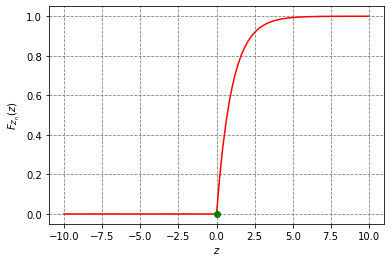
\includegraphics[width=\columnwidth]{stats/solutions/1/figures/cdf.png}
    \caption{cdf of $Z_n$}
    \label{stats/1/fig_cdf}
\end{figure}
\begin{figure}[!ht]
    \centering
    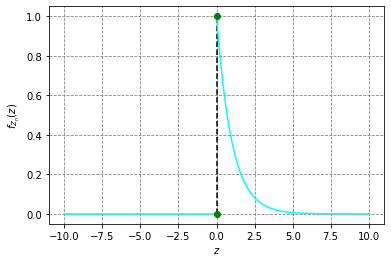
\includegraphics[width=\columnwidth]{stats/solutions/1/figures/pdf.png}
    \caption{pdf of $Z_n$}
    \label{stats/1/fig_pdf}
\end{figure}




%
\item Let $X_1, X_2, \ldots , X_n$ be a random sample of size $n \; ( \geq 2 ) $ from a distribution having the probability density function
\begin{align}
f(x;\theta) = 
\begin{cases}
\dfrac{1}{\theta} \exp\brak{-\dfrac{x}{\theta}} & x > 0, \\
0, & \text{otherwise,}
\end{cases}
\end{align}
where $\theta \in (0, \infty)$. Let $X_{(1)} = $ min $ \{ X_1, X_2, \ldots , X_n \} $ and $T = \sum_{i=1}^n X_i $. Then $E(X_{(1)} | T)$ equals 
\begin{enumerate}[label = (\Alph*)]
\item $\dfrac{T}{n^2}$ \\
\item $\dfrac{T}{n}$ \\
\item $\dfrac{(n+1)T}{2n}$ \\
\item $\dfrac{(n+1)^2 T}{4n^2}$
\end{enumerate}
\solution
\begin{lemma}
    {\em Lehmann–Scheffé theorem :} If $T$ is a complete sufficient statistic for $\theta$ and 
    \begin{align}
    \label{stats/2/eqn 2.0.1}
    E(g(T)) = \tau(\theta)
    \end{align}
    then $g(T)$ is the uniformly minimum-variance unbiased estimator (UMVUE) of $\tau(\theta)$.
    
\end{lemma}




We know that 
\begin{align}
T = \sum_{i=1}^{n} X_i
\end{align}
is a complete and sufficient statistic. By the law of total expectation, 
\begin{align}
\label{stats/2/eqn 2.0.3}
E\brak{E(X_{(1)} | T )} = E(X_{(1)})
\end{align}
By Lehmann–Scheffé theorem, with
\begin{align}
\theta &= X_{(1)},\\ 
\tau(x) &= E(x),\\
g(T) &= E(X_{(1)} | T).
\end{align}
it follows from \eqref{stats/2/eqn 2.0.3} that $E(X_{(1)} | T)$ is the UMVUE of $E(X_{(1)})$.
\begin{align}
\pr{X_{(1)} > x} &= \pr{X_1 > x}\ldots \pr{X_n > x}\\
&= (1-F_{X_{1}}(x))\ldots(1-F_{X_{n}}(x))\\
&= (1-F_{X_{1}}(x))^n \\
&= \exp\brak{-\frac{nx}{\theta}}\\
F_{X_{(1)}}(x) &= 1 - \exp\brak{-\frac{nx}{\theta}}\\
f_{X_{(1)}}(x) &= \frac{n}{\theta} \exp\brak{-\frac{nx}{\theta}}
\end{align}
Therefore, $X_{(1)}$ follows an exponential distribution with mean $\dfrac{\theta}{n}$.
\begin{align}
E(X_{(1)}) = \frac{\theta}{n}
\end{align}
Note that,
\begin{align}
E\brak{\frac{T}{n^2}} &= E\brak{\frac{\sum_{i=1}^n X_i}{n^2}}\\
&= \frac{E(\sum_{i=1}^n X_i)}{n^2}\\
&= \sum_{i=1}^n \frac{E(X_i)}{n^2}\\
&= \sum_{i=1}^n \frac{\theta}{n^2}\\
&= \frac{\theta}{n}\\
&= E(X_{(1)})
\end{align}
Therefore, by Lehmann–Scheffé theorem, with
\begin{align}
\theta &= X_{(1)},\\
\tau(x) &= E(x),\\
g(T) &= \frac{T}{n^2},
\end{align}
it follows that $\dfrac{T}{n^2}$ is UMVUE of $E(X_{(1)})$.\\

Since there exists a unique UMVUE for $E(X_{(1)})$, it follows that 
\begin{align}
E(X_{(1)} | T) = \frac{T}{n^2}
\end{align}
Hence, option A is correct.
\begin{figure}[!hbt]
    \centering
	\includegraphics[width=\columnwidth]{stats/solutions/2/Figures/Figure_1.png}
    \caption{Theory vs Simulated plot of $E(X_{(1)} |T)$}
    \label{stats/2/CDF_Y}
\end{figure}

%
\item Let $X$, $Y$, have the joint discrete distribution such that $X|Y=y \sim$ Binomial($y$, 0.5) and $Y\sim$ Poisson($\lambda$), $\lambda>0$, where $\lambda$ is an unknown parameter. Let $T=T(X, Y)$ be any unbiased estimator of $\lambda$. Then
\begin{enumerate}
    \item  $Var(T) \leq Var(Y)  \text{ for all } \lambda$
    \item $Var(T) \geq Var(Y) \text{ for all } \lambda$
    \item $Var(T) \geq \lambda \text{ for all } \lambda$
    \item $Var(T) = Var(Y) \text{ for all } \lambda$
\end{enumerate}
\solution
\begin{definition}
    {\em Unbiased Estimator: } Suppose we have an estimator $T(X, Y)$; which estimates a parameter $\theta$.  If
    \begin{equation}
        E\brak{T(X, Y)}=\theta
    \end{equation}
    the estimator is unbiased. 
    \end{definition}
    \begin{lemma}
    Since Y has a Poisson distribution, we know that:
    \begin{align}\label{stats/3/Var=lam}
    Var(Y)=\lambda
    \end{align}
    \end{lemma}
    From Bayes Theorem,
    \begin{align}
        \pr{X=x,Y=y}&=\pr{Y=y}  \pr{X=x|Y=y}\\
        &= \comb{y}{x} \frac{1}{2^y} \frac{\lambda^y}{y!} e^{- \lambda}
    \end{align}
    Let us represent $ \pr{X=x,Y=y}$ as a function of $x, y$, and $\lambda$: $f(x, y;\lambda)$.
    \begin{definition} 
    If $T(X, Y)$ is an unbiased estimator of a parameter $\lambda$, the Cramer-Rao bound states that:
    \begin{align}
        Var\brak{T\brak{X,Y}}\geq -\frac{1}{E\brak{\frac{\partial^2 \ln(f(x,y;\lambda))}{\partial\lambda^2}}} \label{stats/3/def CRB}
    \end{align}
    \end{definition}
    From using $\eqref{stats/3/def CRB}$ on $T(X,Y)$,
    \begin{align}
        Var(T(X, Y))&\geq -\frac{1}{E\brak{\frac{\partial^2 \ln(f(x,y;\lambda))}{\partial\lambda^2}}}\\
        &\geq-\frac{1}{E\brak{-\frac{y}{\lambda^2}}}\\
        &\geq\frac{\lambda^2}{E\brak{y}}\\
        &\geq \lambda \label{stats/3/CramerRao}
    \end{align}
    because the expectation value of a Poisson distribution with parameter $\lambda$ is $\lambda$.
    The correct options are options (2) and (3), since by \eqref{stats/3/CramerRao}, we see that 
    \begin{align*}
    Var(T) \geq \lambda=Var(Y)
    \end{align*}
    (from \eqref{stats/3/Var=lam}). (1) and (4) do not hold for all $\lambda$.
    


\item Let $ X_1, \cdots , X_n $ be independent and identically distributed random variables with probability density function
\begin{align}
    f(x) = \frac{1}{2} \lambda^3x^2e^{-\lambda x} ; x>0 ; \lambda > 0
    \label{stats/4/pdf}
\end{align}
Then which of the following statements are true?
\begin{enumerate}
    \item $\dfrac{2}{n} \sum_{i=1}^{n} \dfrac{1}{X_i} $ is an unbiased estimator of $ \lambda$
    \item $\dfrac{3n}{\sum_{i=1}^{n} X_i } $ is an unbiased estimator of $ \lambda$ \\
    \item $\dfrac{2}{n} \sum_{i=1}^{n} \dfrac{1}{X_i} $ is a consistent estimator of $ \lambda$
    \item $\dfrac{3n}{\sum_{i=1}^{n} X_i } $ is a consistent estimator of $ \lambda$
\end{enumerate}
\solution
\begin{definition}
    An \textbf{estimator} is a statistic that estimates some fact about the population.
    The quantity that is being estimated is called the \textbf{estimand.} 
    \end{definition}
    \begin{definition}
    Let $ \Theta = h(X_1,X_2, \cdots, X_n) $  be a point estimator for $ \theta$. The \textbf{bias} of the estimator $ \Theta $ is defined by 
    \begin{align}
        B(\Theta ) = E[\Theta ] - \theta
    \end{align}
    where $ E[\Theta ]$ is the expectation value of the estimator $ \Theta $ and $ \theta$ is the estimand.
    \end{definition}
        \begin{definition}
        Let $\Theta = h(X_1,X_2, \cdots , X_n) $ be a point estimator for a parameter $ \theta $. We say that $ \Theta $ is an \textbf{unbiased estimator} of $ \theta $ if
        \begin{align}
           B(\Theta )= 0 \text{, for all possible values of $\theta$.}
        \end{align}
        \end{definition} 
    \begin{definition}
    Let $ \Theta_1,\Theta_2, \cdots, \Theta_n , \cdots, $  be a sequence of point estimators of $ \theta $. We say that $ \Theta_n $ is a \textbf{consistent} estimator of $ \theta $, if 
    \begin{align}
        \lim_{n\to\infty} \Pr\brak{| \Theta_n - \theta | \ge \epsilon} = 0 \text{ ,for all $ \epsilon > 0$.}
    \end{align}
    \end{definition}
    \begin{definition}
    The \textbf{mean squared error (MSE)} of a point estimator $ \Theta $, shown by $ MSE(\Theta) $, is defined as
    \begin{align}
        MSE(\Theta ) &= E[(\Theta - \theta)^2] \\
        &= Var(\Theta) + B(\Theta)^2
    \end{align}
    where $ B(\Theta ) $ is the bias of $ \Theta $. 
    \end{definition}    
    \begin{theorem}
     Let $ \Theta_1,\Theta_2 , \cdots$ be a sequence of point estimators of $ \theta $. If
    \begin{align}
         \lim_{n\to\infty} MSE( \Theta_n) = 0,
    \end{align}
    then $ \Theta_n $ is a consistent estimator of $ \theta$.
    \end{theorem}
    \textbf{Solving all options : }
    \begin{enumerate}
        \item 
      Now here we have our estimator $ \Theta$ and estimand $ \theta $ as,
     \begin{align}
         \Theta = \dfrac{2}{n} \sum_{i=1}^{n} \dfrac{1}{X_i} \text{  and  }
         \theta = \lambda
     \end{align}
    The expectation value of the estimator is given by, 
    \begin{align}
        E[\Theta ] &= E  \left[   \dfrac{2}{n} \sum_{i=1}^{n} \dfrac{1}{X_i}  \right] \\
        & = \dfrac{2}{n} \sum_{i=1}^{n} E  \left[ \dfrac{1}{X_i}  \right] \\
        & =  \dfrac{2}{n} \sum_{i=1}^{n} \int_{-\infty}^{\infty} \dfrac{1}{x} f(x)\,dx \\
        \label{eq1}
        & = \dfrac{2n}{n} \int_{0}^{\infty} \dfrac{1}{x} \dfrac{1}{2} \lambda^3x^2e^{-\lambda x}\,dx \\
        & = \lambda^3  \int_{0}^{\infty}  x e^{-\lambda x}\,dx \\
        &= \lambda
    \end{align}
    So the bias of estimator is given by,
    \begin{align}
        B(\Theta) &= E[\Theta] - \theta  \\
        &= \lambda - \lambda = 0
    \end{align}
    Therefore $\dfrac{2}{n} \sum_{i=1}^{n} \dfrac{1}{X_i} $ is an unbiased estimator of $ \lambda$ \\
    Option 1 is correct. \\
    \item
     Now in this option we have our estimator $ \Theta$ and quantity to be estimated $ \theta $ as,
     \begin{align}
         \Theta = \dfrac{3n}{\sum_{i=1}^{n} X_i } \text{  and  }
         \theta = \lambda
     \end{align}
    The expectation value of the estimator is given by, 
    \begin{align}
        E[\Theta ] &= E  \left[   \dfrac{3n}{\sum_{i=1}^{n} X_i }  \right] \\
        & = \dfrac{3n}{\sum_{i=1}^{n}}  E  \left[ \dfrac{1}{X_i}  \right] 
    \end{align}
    The value of $  E  \left[ \dfrac{1}{X_i}  \right]  $ can be obtained from \eqref{eq1} as 
    \begin{align} 
         E  \left[ \dfrac{1}{X_i}  \right] = \dfrac{\lambda}{2}
         \label{eq2}
    \end{align}
    So we have,
    \begin{align}
         E[\Theta ] &= \dfrac{3n}{\sum_{i=1}^{n}} \dfrac{\lambda}{2} \\
         &= \dfrac{3n}{n} \dfrac{\lambda}{2} \\
         &= \dfrac{3\lambda}{2}
    \end{align}
    So the bias of estimator is given by,
    \begin{align}
        B(\Theta) &= E[\Theta] - \theta  \\
        &= \dfrac{3\lambda}{2}- \lambda \\
        &= \dfrac{\lambda}{2} \neq 0
    \end{align}
    Therefore $ \dfrac{3n}{\sum_{i=1}^{n} X_i } $ is not an unbiased estimator of $ \lambda$ \\
    Option 2 is not correct. \\
    \item
     Now here we have our estimator $ \Theta$ and quantity to be estimated $ \theta $ as,
     \begin{align}
         \Theta = \dfrac{2}{n} \sum_{i=1}^{n} \dfrac{1}{X_i} \text{  and  }
         \theta = \lambda
     \end{align}
    Now the variance of $ \Theta$ is calculated as
    \begin{align}
        Var(\Theta) &= Var\brak{\dfrac{2}{n} \sum_{i=1}^{n} \dfrac{1}{X_i} } \\
        & = \dfrac{4}{n^2} \sum_{i=1}^{n} Var\brak{\dfrac{1}{X_i}} \\
        \label{eq3}
        & = \dfrac{4n}{n^2} \brak{E  \left[ {\dfrac{1}{X_i}}^2  \right] - {E  \left[ {\dfrac{1}{X_i}}  \right]}^2 } \\
        & = \dfrac{4}{n} \brak{ \int_{-\infty}^{\infty} \dfrac{1}{x^2} f(x)\,dx  - \brak{\dfrac{\lambda}{2}}^2 } \\
        & =  \dfrac{4}{n} \brak{ \int_{0}^{\infty} \dfrac{1}{x^2}  \dfrac{1}{2} \lambda^3x^2e^{-\lambda x} \,dx  - {\dfrac{\lambda^2}{4}} } \\
          & =  \dfrac{4}{n} \brak{ \dfrac{\lambda^3}{2}\int_{0}^{\infty} e^{-\lambda x} \,dx  - {\dfrac{\lambda^2}{4}} } \\ 
        & =  \dfrac{4}{n} \brak{ {\dfrac{\lambda^2}{2}} - {\dfrac{\lambda^2}{4}} } \\ 
        &= \dfrac{\lambda^2}{n}
    \end{align}
    The bias of $ \Theta $ from option 1 is given as
    \begin{align}
        B(\Theta) = 0
    \end{align}
    So we have,
    \begin{align}
        MSE(\Theta_n) &= Var(\Theta) + B(\Theta)^2 \\
        &= \dfrac{\lambda^2}{n}
    \end{align}
    Now,
    \begin{align}
         \lim_{n\to\infty} MSE( \Theta_n) &=    \lim_{n\to\infty} \dfrac{\lambda^2}{n} \\
          &= 0
    \end{align}
    Therefore, $\dfrac{2}{n} \sum_{i=1}^{n} \dfrac{1}{X_i} $ is a consistent estimator of $ \lambda$. 
    Option 3 is correct. \\
    \item 
     Now in this option we have our estimator $ \Theta$ and quantity to be estimated $ \theta $ as,
     \begin{align}
         \Theta = \dfrac{3n}{\sum_{i=1}^{n} X_i } \text{  and  }
         \theta = \lambda
     \end{align}
    Now the variance of $ \Theta$ is calculated as
    \begin{align}
        Var(\Theta) &= Var\brak{\dfrac{3n}{\sum_{i=1}^{n} X_i } } \\
        & = \dfrac{9n^2}{ \sum_{i=1}^{n}} Var\brak{\dfrac{1}{X_i}} \\
    \end{align}
    Now the value of $ Var\brak{\dfrac{1}{X_i}} $ from \eqref{eq3} is substituted, we have
    \begin{align}
         Var(\Theta) &= \dfrac{9n^2}{ \sum_{i=1}^{n}} \dfrac{\lambda^2}{4} \\
         & = \dfrac{9n^2 \lambda^2}{4n }
         & = \dfrac{9n \lambda^2}{4 }
    \end{align}
    The bias of $ \Theta $ from option 2 is given as
    \begin{align}
        B(\Theta) = \dfrac{\lambda}{2}
    \end{align}
    So we have,
    \begin{align}
        MSE(\Theta_n) &= Var(\Theta) + B(\Theta)^2 \\
        &= \dfrac{9n \lambda^2}{4 } + \brak{\dfrac{\lambda}{2}}^2 \\
        & = \dfrac{ \lambda^2}{4 } (9n+1)
    \end{align}
    Now,
    \begin{align}
         \lim_{n\to\infty} MSE( \Theta_n) &=    \lim_{n\to\infty} \dfrac{ \lambda^2}{4 } (9n+1) \\
    \end{align}
    Clearly as n grows larger $ 9n+1$ also grows larger, so
    \begin{align}
         \lim_{n\to\infty} MSE( \Theta_n) \neq 0   
    \end{align}
    Therefore, $\dfrac{3n}{\sum_{i=1}^{n} X_i} $ is not a consistent estimator of $ \lambda$. \\
    Option 4 is not correct. \\
    \end{enumerate}
    \textbf{Therefore option 1 and option 3 are correct.}
%
\item If the marginal probability density function of the $k^{th}$ order statistic of a 
random sample of size 8 from a uniform distribution on $\sbrak{0,2}$ is
\begin{align}
  f(x) =
  \begin{cases}
   \dfrac{7}{32}\,x^{6}\,\brak{2-x},  & 0<x<2, \\ 
         0,               & \text{otherwise,} 
  \end{cases}
\label{stats/qnpdf}
\end{align}
then $k$ equals \underline{\hspace{3cm}}
%
\\
%
\solution
\begin{definition}
    For a given statistical sample $\{X_1, X_2,\cdots X_n\}$, the order statistics is obtained by sorting the
    sample in ascending order. It denoted as $\{X_{(1)}, X_{(2)},\cdots X_{(n)}\}$. The $k^{th}$ smallest value
    $X_{(k)}$ is called  $k^{th}$ order statistic 
    \end{definition}
    \begin{theorem}
    Let $\{X_1, X_2, \cdots X_n\}$ be n i.i.d random variables with common CDF $= F(x)$ and common PDF $= f(x)$, 
    then the marginal probability distribution of $k^{th}$ order statistic (CDF) is denoted by $F_{(k,n)}(x)$ 
    and is given by
    \begin{align}
    F_{(k,n)}(x) =  \sum_{j=k}^{n}\comb{n}{j} \brak{F(x)}^{j}\brak{1-F(x)}^{n-j} \label{stats/5/eqn_1}
    \end{align}
    \label{stats/5/th1}
    \end{theorem}
    \begin{proof}
    %    \begin{align}
        % F_{(k,n)}(x) &= \pr{X_{(k)}\leq x} \\
        % F_{(k,n)}(x) &= \pr{\text{At least k elements have value $\leq x$}} \label{kcdf}
        % \end{align}
        % Since $\pr{X\leq x} = F(x)$ , 
    %     Let $ Q \sim Bern(F(x))$ such that
    %     \begin{align}
    % \pr_Q{q} = \begin{cases}
    %  F(x)  & q = 1\\
    %      1-F(x) & q = 0
    % \end{cases}
%        \end{align}
        Let $P \sim B(n,F(x))$.  Then
        % \begin{align}
        % \pr{P=i} &= \comb{n}{i}\,\pr{Q=1}^{i}\,\pr{Q=0}^{n-i} \\
        % \pr{P=i} &= \comb{n}{i}\,F(x)^{i}\,(1-F(x))^{n-i}\label{bin}  
        % \end{align}
        % Equation \eqref{bin} is probability of exactly $i$ R.V of given sample have values $\leq x$   
        \begin{align}
         F_{(k,n)}(x) &= \pr{P\geq k} \\
         &=  \sum_{j=k}^{n}\comb{n}{j}\, \brak{F(x)}^{j}\,\brak{1-F(x)}^{n-j} 
        \end{align}
        \end{proof}
    \begin{corollary}
    The marginal probability density of $k^{th}$ order statistic (PDF) is denoted by $f_{(k,n)}(x)$  and 
     given by
    \begin{align}
    f_{(k,n)}(x) = n\;\comb{n-1}{k-1}\,f(x)\,(F(x))^{k-1}\,\brak{1-F(x)}^{n-k} \label{stats/5/eqn_2}
    \end{align}
    \label{stats/5/th2}
    \end{corollary}
%
\begin{definition}[Beta function]
    \label{stats/5/def2}
    % The \textbf{Beta function} is defined for $r, s \in \R^{+}$ by 
    \begin{equation}
    B(r,s) = \Int_{0}^{1} x^{r-1}\,\brak{1-x}^{s-1}\,dx = \dfrac{\Gamma(r)\,\Gamma(s)}{\Gamma(r+s)} 
    \label{stats/5/eqn_5}
    \end{equation}
    \end{definition}
    \begin{definition}[Beta Distribution]
    \label{stats/5/bddef}
    The Beta distribution is a continuous distribution defined on the range $(0,1)$ whose PDF given by 
    \begin{align}
    f(x) &= \dfrac{1}{B(r,s)}\,x^{r-1}\,\brak{1-x}^{s-1} 
    \end{align}
    where $\Int_{0}^1f(x) = 1$ as per definition \eqref{stats/5/def2} 
    CDF, Mean value and Variance of Beta distribution
    \begin{align}
     F(x)   &=\dfrac{\Int_{0}^{x}x^{r-1}\,\brak{1-x}^{s-1}}{B(r,s)} =    \dfrac{B_{x}(r,s)}{B(r,s)} \\
     E(x)   &=   \dfrac{r}{r+s} \\
     \var(x) &= \dfrac{rs}{(r+s)^{2}\,(r+s+1)}
    \end{align}
    \end{definition}
    \begin{definition}[Uniform Order Statistics]
    Let $\{X_1,\cdots X_n\}$ be i.i.d form a uniform distribution on $[0,1]$ such that $f_{X}(x) = 1$ and $F_{X}(x)=x$.
    From Theorem \eqref{stats/5/th2}, equation \eqref{stats/5/eqn_2}
    \begin{align}
    f_{(k,n)}(x) &= n\;\comb{n-1}{k-1}\,x^{k-1}\,\brak{1-x}^{n-k}\label{stats/5/eqn_3}
    \end{align}
    \end{definition}
    \begin{lemma}
    \label{stats/5/lma}
    Uniform order statistics on [0,1] the PDF of $k^{th}$ order statistic follows Beta distribution with $r=k$, $s=n-k+1$
    and  PDF is given by 
    \begin{align}
    f_{(k,n)}(x) &= \dfrac{1}{B(k,n-k+1)}\,x^{k-1}\,\brak{1-x}^{(n-k+1)-1} 
    \end{align}
    \end{lemma}
    \newpage
    \begin{proof}
    Since  \eqref{stats/5/eqn_3} is the PDF,
    \begin{equation}
     \Int_{0}^{1} n\;\comb{n-1}{k-1}\,x^{k-1}\,\brak{1-x}^{n-k} \,dx  = 1    
    \end{equation}
    \begin{align}
    \Int_{0}^{1} x^{k-1}\brak{1-x}^{n-k} \,dx  &= \dfrac{(k-1)!\,(n-k)!}{n!}  \\
    \Int_{0}^{1} x^{k-1}\brak{1-x}^{n-k} \,dx  &= \dfrac{\Gamma(k)\,\Gamma(n-k+1)}{\Gamma\brak{k+(n-k+1))}} \\
    \Int_{0}^{1} x^{k-1}\brak{1-x}^{n-k} \,dx  &= B(k,n-k+1) \\
    \Int_{0}^{1} \dfrac{x^{k-1}\brak{1-x}^{(n-k+1)-1}}{B(k,n-k+1)}\,dx  &= 1
    \end{align}
    from definition \eqref{stats/5/bddef} with $r=k$ and $s=n-k+1$ equation \eqref{stats/5/eqn_3} follows beta distribution
    \end{proof}
    From lemma \eqref{stats/5/lma}, PDF of $k^{th}$ order statistic of a uniform distribution on $[0,1]$ follows 
    beta distribution
    \begin{align}
    \Int_{0}^{2}f_{(k,8)}(x)\,dx &= \Int_{0}^{2} \dfrac{7}{32}\,x^{6}\,\brak{2-x}\,dx \\
    \Int_{0}^{2}f_{(k,8)}(x)\,dx &= \Int_{0}^{2} 56\,\brak{\dfrac{x}{2}}^{6}\,\brak{1-\dfrac{x}{2}}\,d\brak{\dfrac{x}{2}}
    \end{align}
    Let new random variable be $t$ such that $t=x/2$, New sample be $\{T_1,\cdots T_8\}$ such that $T_{i}=X_{i}/2$.
    \begin{align}
    f_{(k,8)}(t) &= 56\,t^{6}\,\brak{1-t} \\
    \Int_{0}^{2}f_{(k,8)}(x)\,dx &=  \Int_{0}^{1}f_{(k,8)}(t)\,dt = 1
    \end{align}
    The Uniform distribution of new random sample is on $[0,1]$ such that   PDF $= 1$ and CDF $= t$ 
    $f(k,8)(x)$ 
    %in equation \eqref{stats/5/qnpdf}  (after conversion)
    \begin{align}
    f_{(k,8)}(t) =
      \begin{cases}
          56\,t^{6}\,\brak{1-t},  & 0<t<1, \\ 
          \hspace{1cm}   0,               & \text{otherwise,} 
      \end{cases}
      \label{stats/5/pdf_t}
    \end{align}
    Since equation \eqref{stats/5/pdf_t} is a Beta distribution with $r=k$, $s=n-k+1$  
    \begin{align}
    r-1 = k-1 &= 6 \\
    \therefore k &= 7 
    \end{align}
    Hence the \textbf{value of k is 7}


    
\item Let $X_1, X_2, \ldots , X_n$ be a random sample of size $n \; ( \geq 2 ) $ from a distribution having the probability density function
\begin{align}
f(x;\theta) = 
\begin{cases}
\dfrac{1}{\theta} \exp\brak{-\dfrac{x}{\theta}} & x > 0, \\
0, & \text{otherwise,}
\end{cases}
\end{align}
where $\theta \in (0, \infty)$. Let $X_{(1)} = $ min $ \{ X_1, X_2, \ldots , X_n \} $ and $T = \sum_{i=1}^n X_i $. Then $E(X_{(1)} | T)$ equals $\ldots \ldots \ldots$
\begin{enumerate}[label = (\Alph*)]
\item $\dfrac{T}{n^2}$ \\
\item $\dfrac{T}{n}$ \\
\item $\dfrac{(n+1)T}{2n}$ \\
\item $\dfrac{(n+1)^2 T}{4n^2}$
\end{enumerate}
%
\solution
\begin{lemma}[Sum of Gamma random variables]
    \label{stats/4/gamma}
Suppose that $X_i \sim \Gamma(k, \theta), i = 1, \dots, n$. Then $T = \sum_{i=1}^{n} X_i \sim \Gamma(nk, \theta)$.
\end{lemma}
\begin{definition}[Laplace transform]
    Laplace transform is an integral transform that converts a real function of a real variable $t$ to a function of a complex variable $s$. The laplace transform of a function $f(t)$ evaluated at $s$ is defined by
    \begin{align}
    F(s) = \int_0^{\infty} f(t) e^{-st} dt
    \end{align}
    \end{definition}
    \begin{lemma}
    \label{stats/6/lemma_laplace_transform}
    If the laplace transform of a function $f(t)$ at $s$ is $0$ for all $s>0$, then the function $f(t) = 0$ almost everywhere in $(0, \infty)$.
    \end{lemma}
\begin{definition}[Complete Statistic]
The statistic $T$ is said to be complete for the distribution of $X$ if, for every measurable function $g$, if
\begin{align}
E(g(T)) = 0 \; \forall \; \theta \Rightarrow \pr{g(T)=0} = 1 
\end{align}
\end{definition}
\begin{definition}[Sufficient Statistic]
A statistic $t = T(X)$ is sufficient for underlying parameter $\theta$ precisely if the conditional probability distribution of the data $X$, given the statistic $t = T(X)$, does not depend on the parameter $\theta$. 
\end{definition}
\begin{theorem}[Fischer-Neymann Factorisation theorem]
If the probability density function is $f_\theta (x)$, then $T$ is sufficient for $\theta$ if and only if nonnegative functions $g$ and $h$ can be found such that
\begin{align}
f_\theta (x) = h(x)g_\theta(T(x))
\end{align}
\end{theorem}
\begin{lemma} \label{stats/6/lemma_sufficient_complete}
\begin{align}
T = \sum_{i=1}^{n} X_i
\end{align}
is a complete and sufficient statistic. 
\end{lemma}
\begin{proof}
\begin{enumerate}
\item \textit{(Sufficiency)}
\begin{align}
f_{X}(x_1, x_2, \ldots x_n) &= \prod_{i=1}^{n}f_{X_i}(x_i)\\
&= \prod_{i=1}^{n} \dfrac{1}{\theta} \exp\brak{-\dfrac{x_i}{\theta}} \\
&= 1 \cdot \dfrac{1}{\theta^n} \exp\brak{-\dfrac{T}{\theta}}\\
&= h(X) \cdot g(T, \theta) 
\end{align}
with 
\begin{align}
g(T, \theta) &= \dfrac{1}{\theta^n} \exp\brak{-\dfrac{T}{\theta}}\\
h(X) &= 1
\end{align}
Therefore, $T$ is a sufficient statistic.
\item \textit{(Completeness)}
From Lemma     \ref{stats/4/gamma}, $X_i \sim \Gamma \brak{1, \frac{1}{\theta}} \implies  T = \sum_{i=1}^n X_i \sim \Gamma \brak{n, \frac{1}{\theta}}$. 
\begin{align}
\therefore E(g(T)) &= 
\int_0 ^{\infty} g(t) \dfrac{t^{n-1} e^{-\frac{t}{\theta}}}{\theta^n(n-1)!} dt\\ 
&= \frac{1}{\theta^n (n-1)!} \int_0 ^{\infty} g(t) t^{n-1} e^{-\frac{t}{\theta}} dt\\ 
&= \frac{1}{\theta^n (n-1)!} F \brak{\frac{1}{\theta}}
%&= 0 \text{ for all } \theta > 0.
\end{align}
where, 
\begin{align}
f(t) &= t^{n-1}g(t) \xrightleftharpoons[]{\mathcal{L}} F \brak{\frac{1}{\theta}}
% &= \text{Laplace Transform of} f(t) \text{ at } \theta
\end{align}
is the Laplace transform relationship.
Then
\begin{align}
E\brak{g(T)}=0 \forall \theta > 0 \implies F \brak{\frac{1}{\theta}} = 0 \forall  \theta > 0
\label{stats/6/eqn}
\\ \implies 
f(t)=0 \text{ a.e } (0, \infty)\\
\text{or, }g(t)=0 \text{ a.e }(0, \infty)\\
\implies \pr{g(t)=0} = 1
\end{align}
from Lemma     \ref{stats/6/lemma_laplace_transform}.  
$\therefore T$ is a complete statistic.
\end{enumerate}
\end{proof}
\begin{theorem}[Lehmann–Scheffé theorem]
If $T$ is a complete sufficient statistic for $\theta$ and 
\begin{align}
\label{eqn 2.0.1}
E(g(T)) = \tau(\theta)
\end{align}
then $g(T)$ is the uniformly minimum-variance unbiased estimator (UMVUE) of $\tau(\theta)$.
\end{theorem}
%
\begin{proposition} \label{stats/6/prop_3.1}
$E(X_{(1)}|T)$ is the uniformly minimum-variance unbiased estimator (UMVUE) of $E(X_{(1)})$
\end{proposition}
\begin{proof}
By the law of total expectation, 
\begin{align}
\label{stats/6/eqn 2.0.3}
E\brak{E(X_{(1)} | T )} = E(X_{(1)})
\end{align}
We know that $T = \sum_{i=1}^n X_i$ is a complete and sufficient statistic by Lemma \ref{stats/6/lemma_sufficient_complete}. By Lehmann–Scheffé theorem, with
\begin{align}
\theta &= X_{(1)},\\ 
\tau(x) &= E(x),\\
g(T) &= E(X_{(1)} | T).
\end{align}
it follows from \eqref{stats/6/eqn 2.0.3} that $E(X_{(1)} | T)$ is the UMVUE of $E(X_{(1)})$.
\end{proof}
\begin{proposition} \label{stats/6/prop_3.2}
$\frac{T}{n^2}$ is uniformly minimum-variance unbiased estimator (UMVUE) of $E(X_{(1)})$
\end{proposition}
\begin{proof}
\begin{enumerate}
\item Let's find the probability distribution function and the expectation value of $X_{(1)}$ : 
\begin{align}
\pr{X_{(1)} > x} &= \pr{X_1 > x}\ldots \pr{X_n > x}\\
&= (1-F_{X_{1}}(x))\ldots(1-F_{X_{n}}(x))\\
&= (1-F_{X_{1}}(x))^n \\
&= \exp\brak{-\frac{nx}{\theta}}\\
F_{X_{(1)}}(x) &= 1 - \exp\brak{-\frac{nx}{\theta}}\\
f_{X_{(1)}}(x) &= \frac{n}{\theta} \exp\brak{-\frac{nx}{\theta}}
\end{align}
Therefore, $X_{(1)}$ follows an exponential distribution with mean $\dfrac{\theta}{n}$.
\begin{align}
E(X_{(1)}) = \frac{\theta}{n}
\end{align}
\item $\frac{T}{n^2}$ is uniformly minimum-variance unbiased estimator (UMVUE) of $E(X_{(1)})$, since $E\brak{\frac{T}{n^2}} = E(X_{(1)})$ : \\
Note that,
\begin{align}
E\brak{\frac{T}{n^2}} &= E\brak{\frac{\sum_{i=1}^n X_i}{n^2}}\\
&= \frac{E(\sum_{i=1}^n X_i)}{n^2}\\
&= \sum_{i=1}^n \frac{E(X_i)}{n^2}\\
&= \sum_{i=1}^n \frac{\theta}{n^2}\\
&= \frac{\theta}{n}\\
&= E(X_{(1)})
\end{align}
\end{enumerate}
Therefore, by Lehmann–Scheffé theorem, with
\begin{align}
\theta &= X_{(1)},\\
\tau(x) &= E(x),\\
g(T) &= \frac{T}{n^2},
\end{align}
it follows that $\dfrac{T}{n^2}$ is UMVUE of $E(X_{(1)})$.\\
\end{proof}
Since there exists a unique UMVUE for $E(X_{(1)})$, it follows from Proposition \ref{stats/6/prop_3.1} and Proposition \ref{stats/6/prop_3.2} that 
\begin{align}
E(X_{(1)} | T) = \frac{T}{n^2} 
\end{align}
Hence, option A is correct.
\begin{figure}[!hbt]
    \centering
	\includegraphics[width=\columnwidth]{stats/solutions/6/Figures/Figure_1.png}
    \caption{Theory vs Simulated plot of $E(X_{(1)} |T)$}
    \label{CDF_Y}
\end{figure}


\item Let $X_1,X_2,...,X_n$ be independent and identically distributed Bernoulli($\theta$), where $0<\theta<1$ and $n>1$. Let the prior density of $\theta$ be proportional to $\frac{1}{\sqrt{\theta\,(1-\theta)}}$, $0<\theta<1$. Define $S=\sum_{i=1}^nX_i$.\\[1pt] Then valid statements among the following are:
\begin{enumerate}[label = \arabic*.]
    \item The posterior mean of $\theta$ does not exist;
    \item The posterior mean of $\theta$ exists;
    \item The posterior mean of $\theta$ exists and it is larger than the maximum likelihood estimator for all values of S.
    \item The posterior mean of $\theta$ exists and it is larger than the maximum likelihood estimator for some values of S.
\end{enumerate}
\solution
\begin{definition}[Posterior Mean]
    Posterior mean is the mean of the posterior distribution of $\theta$, i.e., 
    \begin{align}
        E\brak{\theta|X} = \int{\theta\;f\brak{\theta|X}\,d\theta}\label{stats/7/eq5}
    \end{align}
    \end{definition}
    \begin{definition}[Beta Function]
    The beta function, $B\brak{x,y}$, is defined by the integral
    \begin{align}
        B\brak{x,y} &= \int_0^1 t^{x-1}\,\brak{1-t}^{y-1}\,dt\nonumber\\
        &= \frac{x+y}{xy}\times \frac{1}{\comb{x+y}{x}}\label{stats/7/eq1}
    \end{align}
    where $Re\brak{x}>0$ and $Re\brak{y}>0$.
    \end{definition}
    
    \begin{lemma}
        Let $f\brak{\theta}$ be the prior density of $\theta$.  Then 
    \begin{align}
        f\brak{\theta} = \frac{\theta^{-\frac{1}{2}}\,\brak{1-\theta}^{-\frac{1}{2}}}{B\brak{\frac{1}{2},\frac{1}{2}}}\label{stats/7/eq6}
    \end{align}
    \end{lemma}
    \begin{proof}
    \begin{align}
        &f\brak{\theta} \propto \frac{1}{\sqrt{\theta\,\brak{1-\theta}}}\nonumber\\
        \implies &f\brak{\theta} = \frac{K}{\sqrt{\theta\,\brak{1-\theta}}}
    \end{align}
    where $K$ is the proportionality constant.
    \begin{align}
        &\int_0^1 f\brak{\theta}\,d\theta = 1\nonumber\\
        \implies &K\;\int_0^1 \frac{1}{\sqrt{\theta\,\brak{1-\theta}}}\,d\theta =1
    \end{align}
    From \eqref{stats/7/eq1} we get,
    \begin{align}
        &K\times B\brak{\frac{1}{2},\frac{1}{2}} = 1\nonumber\\
        \implies &K = \frac{1}{B\brak{\frac{1}{2},\frac{1}{2}}}\\
        \therefore\, &f\brak{\theta} = \frac{\theta^{-\frac{1}{2}}\,\brak{1-\theta}^{-\frac{1}{2}}}{B\brak{\frac{1}{2},\frac{1}{2}}}
    \end{align}
    \end{proof}
    \begin{definition}[Likelihood Function]
    The likelihood function is defined as 
    \begin{align}
        f\brak{\vec{X}|\theta} = \prod_{i=1}^n f\brak{X_i|\theta}\label{stats/7/eq8}
    \end{align}
    \end{definition}
    \begin{lemma}
    \begin{align}
        f\brak{\vec{X}|\theta}=\theta^S\,\brak{1-\theta}^{n-S}\label{stats/7/eq7}
    \end{align}
    \end{lemma}
    \begin{proof}
    From \eqref{stats/7/eq8} we get,
    \begin{align}
        f\brak{\vec{X}|\theta} &= \prod_{i=1}^n\theta^{X_i}\,\brak{1-\theta}^{1-X_i}\nonumber\\
        &=\theta^S\,\brak{1-\theta}^{n-S}
    \end{align}
    \end{proof}
    \begin{definition}[Maximum Likelihood Esitmator]
    The maximum likelihood estimator is the value which maximizes the likelihood function, i.e.,
    \begin{align}
        \text{MLE} = \text{arg$_{\theta \in (0,1)}$ max}\brak{f\brak{\vec{X}|\theta}}
    \end{align}
    \end{definition}
    \begin{lemma}
    \begin{align}
        \text{MLE} = \frac{S}{n}
    \end{align}
    \end{lemma}
    \begin{proof}
    Using log of likelihood function in \eqref{stats/7/eq7} and differentiating,  we get,
    \begin{align}
        &\ln\brak{{f\brak{\vec{X}|\theta}}} = S\ln\brak{{\theta}} + \brak{n-S}\ln\brak{{1-\theta}}\\
        &\frac{\partial \ln\brak{{f\brak{X|\theta}}}}{\partial \theta} = \frac{S}{\theta} + \frac{S-n}{1-\theta} = 0 \nonumber\\
         \therefore\, &\text{MLE} = \frac{S}{n}
    \end{align}
    \end{proof}
    % \begin{definition}
    % The marginal distribution of $X$ is given by
    % \begin{align}
    %     f\brak{X} = \int f\brak{X,Y}\,dY\label{stats/7/eq9}
    % \end{align}
    %\end{definition}
    \begin{definition}[Posterior Density]
    The posterior density of $\theta$ is defined as 
    \begin{align}
        f\brak{\theta|\vec{X}} = \frac{f\brak{\vec{X},\theta}}{f\brak{\vec{X}}}
    \end{align}
    \end{definition}
    \begin{lemma}
    \begin{align}
        f\brak{\theta|\vec{X}} = \frac{\theta^{S-\frac{1}{2}}\,\brak{1-\theta}^{n-S-\frac{1}{2}}}{B\brak{S+\frac{1}{2},n-S+\frac{1}{2}}}
    \end{align}
    \end{lemma}
    \begin{proof}
    Using Bayes' theorem, 
    \begin{align}
        f\brak{\theta|X} &= \frac{f\brak{\vec{X},\theta}}{\int_0^1 f\brak{\vec{X},\theta}\,d\theta} \nonumber\\
        &= \frac{f\brak{\vec{X}|\theta}\, f\brak{\theta}}{\int_0^1 f\brak{\vec{X}|\theta}\, f\brak{\theta}\,d\theta}\label{stats/7/eq10}
    \end{align}
    Using \eqref{stats/7/eq6} and \eqref{stats/7/eq7} in \eqref{stats/7/eq10} we get,
    \begin{align}
        f\brak{\theta|\vec{X}} &= \frac{\theta^{S-\frac{1}{2}}\,\brak{1-\theta}^{n-S-\frac{1}{2}}}{\int_0^1 \theta^{S-\frac{1}{2}}\,\brak{1-\theta}^{n-S-\frac{1}{2}}\,d\theta}
    \end{align}
    Using \eqref{stats/7/eq1} we get,
    \begin{align}
        f\brak{\theta|\vec{X}} = \frac{\theta^{S-\frac{1}{2}}\,\brak{1-\theta}^{n-S-\frac{1}{2}}}{B\brak{S+\frac{1}{2},n-S+\frac{1}{2}}}
    \end{align}
    \end{proof}
    \begin{corollary}
    \begin{align}
        E\brak{\theta|\vec{X}} = \frac{S+\frac{1}{2}}{n+1}\label{stats/7/eq3}
    \end{align}
    \end{corollary}
    \begin{proof}
    From \eqref{stats/7/eq5} we get,
    \begin{align}
        E\brak{\theta|\vec{X}} &= \int_0^1 \theta\;f\brak{\theta|\vec{X}}\,d\theta\nonumber\\
        &=\int_0^1 \frac{\theta^{S+\frac{1}{2}}\,\brak{1-\theta}^{n-S-\frac{1}{2}}}{B\brak{S+\frac{1}{2},n-S+\frac{1}{2}}}\,d\theta\nonumber\\
        &=\frac{B\brak{S+\frac{3}{2},n-S+\frac{1}{2}}}{B\brak{S+\frac{1}{2},n-S+\frac{1}{2}}}\label{stats/7/eq2}
    \end{align}
    Using \eqref{stats/7/eq1} in \eqref{stats/7/eq2} we get
    \begin{align}
        E\brak{\theta|\vec{X}} = \frac{S+\frac{1}{2}}{n+1}
    \end{align}
    \end{proof}
    \begin{corollary}
    For $E\brak{\theta|\vec{X}}$ to be greater than MLE,
    \begin{align}
        n>2\,S\label{stats/7/eq4}
    \end{align}
    \end{corollary}
    \begin{proof}
    \begin{align}
        &\frac{S+\frac{1}{2}}{n+1} > \frac{S}{n}\nonumber\\
         \therefore\;&n>2\,S
    \end{align}
    \end{proof}
    \begin{enumerate}
        \item From \eqref{stats/7/eq3} we get 
            \begin{align*}
            E\brak{\theta|\vec{X}} = \frac{S+\frac{1}{2}}{n+1} 
            \end{align*}
            $\implies$ for $ E\brak{\theta|\vec{X}}$ to exist, 
            \begin{align*}
                n\neq-1
            \end{align*}
            Given in the question,
            \begin{align*}
                n>1
            \end{align*}
             $\implies E\brak{\theta|\vec{X}}$ exists.\\
             $\therefore$ Option 2 is correct and option 1 is incorrect.
        \item From \eqref{stats/7/eq4} we get 
            \begin{align*}
                E\brak{\theta|\vec{X}}>\, \text{MLE}\\
            \end{align*}
            when
            \begin{align*}
                n>2\,S
            \end{align*}
            $\implies E\brak{\theta|\vec{X}}>\, $MLE for some values of S.\\
            $\therefore$ Option 4 is correct and option 3 is incorrect.
    \end{enumerate}
    $\therefore$ Option 2 and 4 are correct.
%
\item Let $X_1,X_2,X_3,X_4,X_5$ be independent and identically distributed random variables each following a uniform distribution on (0,1) and M denote their median. Then which of the following statements are true?
\begin{enumerate}
    \item $\pr{M<\frac{1}{3}}=\pr{M>\frac{2}{3}}$\\
    \item $M$ is uniformly distributed on (0,1)\\
    \item $E(M)=E(X_1)$\\
    \item $V(M)=V(X_1)$
\end{enumerate}
\solution
\begin{theorem}[Uniform distribution]
    A random variable $X$ is said to be uniformly distributed in $a\leq x\leq b$ if its density function is
    \begin{align}
        f(x)=
        \begin{cases}
        \frac{1}{b-a} & \text{if } a\leq x \leq b\\
        0 & \text{otherwise}
        \end{cases}\label{stats/8/eq:1}
    \end{align}
    and the distribution is called uniform distribution.
    The mean and variance are respectively,
    \begin{align}
        \mu=\frac{a+b}{2}\label{stats/8/eq:2}
    \end{align}
    \begin{align}
         \sigma^2=\frac{(b-a)^2}{12}\label{stats/8/eq:3}
    \end{align}
    \label{stats/8/theorem}
    \end{theorem}
    \begin{theorem}[Beta distribution]
    The Beta distribution is a continuous distribution defined on the range
    (0, 1) where 
    %the parameters are given by\\
    %If $X\sim B(r,s)$, where $B(r,s)$ is a beta function
    \begin{align}
      \label{stats/8/eq:4}  f_X(x)&=\frac{1}{B(r,s)}x^{r-1}(1-x)^{s-1}\\ 
        \label{stats/8/eq:5}F_X(x)&=\int_{0}^{x}\frac{1}{B(r,s)}x^{r-1}(1-x)^{s-1}dx=\frac{B_x(r,s)}{B(r,s)}\\ 
      \label{stats/8/eq:6}  B(r,s)&=\int_{0}^{1}x^{r-1}(1-x)^{s-1}dx=\frac{(r-1)!(s-1)!}{(r+s-1)!}\\ 
         \label{stats/8/eq:7}B_x(r,s)&=\int_{0}^{x}x^{r-1}(1-x)^{s-1}dx\\
       \label{stats/8/eq:8} E(X)&=\frac{r}{r+s}\\ 
        \label{stats/8/var} Var(X)&=\frac{rs}{(r+s)^{2}(r+s+1)} 
    \end{align}
    and $B(r,s)$ is the beta function. 
    \end{theorem}
    \begin{definition}[Order statistics]
    For a given statistical sample $\{X_1, X_2,\cdots X_n\}$, the order statistics is obtained by sorting the sample in ascending order. It denoted as $\{X_{(1)}, X_{(2)},\cdots X_{(n)}\}$.
    \end{definition}
    \begin{definition}[Median of order statistics]
    Median is defined as the middle number of a sorted sample. It is denoted by M and defined using order statistics of a sample as
    \begin{align}
      M =
      \begin{cases}
       X_{((n+1)/2)},                                           &\text{if $n$ is odd,} \\ \\
      \dfrac{ X_{(n/2)} + X_{(n/2+1)}}{2} ,                     &\text{if $n$ is even,} 
      \end{cases}
    \end{align}
    \label{stats/8/median}\label{stats/8/def2}
    \end{definition}
    \begin{remark}
    The order statistics of the uniform distribution on the unit interval have marginal distributions belonging to the Beta distribution family.
    \begin{align}
    X_{(k)} \sim B(k,n+1-k)
    \end{align}\label{stats/8/rem}
    \end{remark}
    \begin{enumerate}
     \item 
    From definition \eqref{stats/8/median} median $M$ is given by
    \begin{align}
      M &= X_{((5+1)/2)}\\
      &=X_{(3)}\label{stats/8/eq:m}
    \end{align}
    From remark \eqref{stats/8/rem} 
    \begin{align}
    X_{(3)} \sim B(3,3)
    \end{align}
    From \eqref{stats/8/eq:6}
    \begin{align}
        B(3,3)&=\frac{(3-1)!(3-1)!}{(3+3-1)!}=\frac{1}{30}
     \end{align}
     From \eqref{stats/8/eq:4}
     \begin{align}
         f(x)=30x^{2}(1-x)^{2}
     \end{align}
     From \eqref{stats/8/eq:5}
     \begin{align}
         F(x)&=\int_{0}^{x}30x^{2}(1-x)^{2}dx\\
         &=30x^{3}\brak{\frac{1}{3}+\frac{x^2}{5}-\frac{x}{2}}
     \end{align}
     \begin{align}
         \pr{M<\frac{1}{3}}&=F\brak{\frac{1}{3}}=0.20987\\
         \pr{M>\frac{2}{3}}&=F(1)-F\brak{\frac{2}{3}}=0.20987
     \end{align}
     \begin{align}
          \therefore \pr{M<\frac{1}{3}}=\pr{M>\frac{2}{3}}
     \end{align}
      Hence \textbf{Option 1 is true.}
        
        
        
        
     \item From \eqref{stats/8/eq:m}, median M is a third order statistic. Clearly from remark \eqref{stats/8/rem}, $M$ is not an uniform distribution.
    \\Hence \textbf{Option 2 is false.}
    \item From \eqref{stats/8/eq:1}
    \begin{align}
        f(x)=
        \begin{cases}
        1 & \text{if } 0\leq x \leq 1\\
        0 & \text{otherwise}
        \end{cases}
    \end{align}
    From \eqref{stats/8/eq:2} 
    \begin{align}
        E(X_1)&=\frac{1}{2}
    \end{align}
    From \eqref{stats/8/eq:8}
    \begin{align}
        E(M)=\frac{3}{3+3}=\frac{1}{2}
    \end{align}
     \begin{align}
          \therefore E(M)=E(X_1)
     \end{align}
       Hence \textbf{Option 3 is true.}
    \item From \eqref{stats/8/eq:3}
    \begin{align}
          V(X_1)&=\frac{1}{12}
    \end{align}
    From \eqref{stats/8/var}
    \begin{align}
        V(M)=\frac{1}{28}
    \end{align}
    \begin{align}
          \therefore V(M)\neq V(X_1)
     \end{align}
       Hence \textbf{Option 4 is false.}
    \end{enumerate}

\item Suppose n units are drawn from a population of N units sequentially as follows. A random sample
\begin{align}
    U_1, U_2, ... U_N \text{ of size N, drawn from }U\brak{0, 1} 
\end{align} 
The k-th population unit is selected if 
\begin{align}
    U_k<\frac{n - n_k}{N-k+1}, k = 1, 2, ..N. \text{where, } n_1=0, n_k = 
\end{align}
number of units selected out of first k-1 units for each k = 2, 3, ..N. Then,
\begin{enumerate}
    \item The probability of inclusion of the second unit in the sample
    \begin{align}
        \text{ is } \frac{n}{N}
    \end{align}
    \item The probability of inclusion of the first and the second unit in the sample
    \begin{align}
        \text{ is } \frac{n \brak{n-1}}{N \brak{N-1}}
    \end{align}
    \item The probability of not including the first and including the second unit in the sample
    \begin{align}
        \text{ is } \frac{n \brak{N-n}}{N \brak{N-1}}
    \end{align}
    \item The probability of including the first and not including the second unit in the sample
    \begin{align}
        \text{ is } \frac{n \brak{n-1}}{N \brak{N-1}}
    \end{align}
\end{enumerate}
%
\solution
\input{solutions/2018/dec/116.tex}
%
%
\item Let $X_{1},X_{2},X_{3},..,X_{n}$ be independent random variables follow a common continuous distribution \textbf{F}, which is symmetric about 0. For i=1,2,3,..n, define 
\begin{align}
\tag{1.1}
\label{eq1}
S_{i} = 
\begin{cases}
1 & if \hspace{0.2cm}X_{i}>0
\\
-1 & if\hspace{0.2cm} X_{i}<0 \hspace{0.2cm} and
\\
0 & if \hspace{0.2cm}X_{i}=0
\end{cases}
\end{align}
$R_{i}$=rank of $|X_{i}|$ in the set\{$|X_{1}|,|X_{2}|,..,|X_{n}|$\}.Which of the following statements are correct?
\begin{enumerate}
\item $S_{1},S_{2},..,S_{n}$ are independent and identically distributed.
\item $R_{1},R_{2},..,R_{n}$ are independent and identically distributed.
\item $S=\brak{S_{1},S_{2},..,S_{n}}$ and $R=\brak{ R_{1},R_{2},..,R_{n}}$ are independent.
\end{enumerate}
%
\solution

A sequence $\{X_{i}\}$ is an Independent and identical if and only if 
$F_{X_{n}}(x)=F_{X_{k}}(x)$
$\forall$ n,k,x and any subset of terms of the sequence is a set of mutually independent random variables.
Where F is the probability density function.
\begin{enumerate}
\item As the probability distribution function of $\{X_{i}\}$ is symmetric about origin we can say that 
\begin{equation}
\tag{2.1}
  F_{X_{i}}(-x)=F_{X_{i}}(x)    \forall x \in R  
\end{equation}
and the mean of the distribution($\mu$)
\begin{equation}
    \tag{2.2}
    \mu=0
\end{equation}
The sequence $S_{i}$ depend on $X_{i}$ as mention in \ref{eq1}, as each $S_{i}$ depend only on $X_{i}$ we can say that sequence $S_{i}$ is independent.
\begin{equation}
    \tag{2.3}
\pr{S_{1}=1,S_{2}=1,...,S_{n}=1}=\Pi_{i=1}^{n}\pr{S_{i}=1}
\end{equation}
Any subset of terms of sequence $\{S_{i}\}$ is a set of mutually independent random variables and its distribution is identical. 
\begin{align}
    \tag{2.4}
    F_{S_{n}}(s)=F_{S_{k}}(s) \hspace{0.5cm} \forall s,k,n
\end{align}
So, the sequence $\{S_{i}\}$ is independent and identical.
\item 
\textbf{Ranking} refers to the data transformation in which the numerical or ordinary values are replaced by the rank of numerical value when compared to a list of other values.Usually we follow increasing order for ranking.\\
Ranking of a sequence depend on every elements of the sequence.Let $\{R_{i}\}$ be the output sequence of the ranking function of $\{|X_{i}|\}$.
\begin{equation}
    \tag{2.5}
    R_{k}=\text{rank of $|X_{k}|$ in the set\{$|X_{1}|,|X_{2}|,..,|X_{n}|$\}}
\end{equation}
As $R_{k}$ depend not only on $|X_{k}|$ but on the rest of the elements of the set\{$|X_{1}|,|X_{2}|,..,|X_{n}|$\}. So the sequence $R_{i}$ is not independent. Hence $R_{i}$ is not an independent and identical distribution.
\item 
As the $i^{th}$ element of sequence R depends only on set\{$|X_{1}|,|X_{2}|,..,|X_{n}|$\}, we can say that sequence S and R are independent.
\end{enumerate}
Answer:A,C
%
%
\item A simple random variable of size n will be drawn from a class of 125 students, and the mean mathematics score of the sample will be computed, If the standard error of the sample mean for "with replacement sampling" is twice as much as the standard error of the sample mean for "without replacement sampling", the value of n is ? 
	\begin{enumerate}
	\item 32
	\item 63
	\item 79
	\item 94
	\end{enumerate}
%
\solution
Let N be the population size so, N=120. The given sample size is n.
\textbf{Notations :}
y : student under consideration.
$y_i$ : Maths marks of $i^{th}$ student in the sample.
Y : student of class.
$Y_i$ : Maths marks of $i^{th}$ student in the class.
$\overline{y}=\dfrac{1}{n}\sum_{i=1}^{n}y_i$ : Average of sample class.
$\overline{Y}=\dfrac{1}{N}\sum_{i=1}^{N}Y_i$ : Average of whole class.
$S^2 = \dfrac{1}{N-1} \sum_{i=1}^{N} (Y_i-\bar{Y})^2$ : S=Std dev of the class.
$\sigma^2=\dfrac{1}{N} \sum_{i=1}^{N} (Y_i-\bar{Y})^2$ : Variance of the class.
Standard error of sample mean $SE_{mean}=\dfrac{s}{\sqrt{n}}$.\\
Where 
\begin{align*}
s & = \text{standard deviation of sample mean.}\\
n & = \text{sample class size.}
\end{align*}
\textbf{Variance of the $\overline{y}$}
\begin{align}
& V(\overline{y})= E(\overline{y}-\overline{Y})^2\\
& = E\left[\dfrac{1}{n} \sum_{i=1}^{n}(y_i-\overline{Y})\right]^2\\
& = E\left[\dfrac{1}{n^2} \sum_{i=1}^{n} (y_i-\overline{Y})^2 + \dfrac{1}{n^2} \underset{1\leq i\neq j\leq n}{\sum\sum}\, (y_i-\overline{Y})(y_j-\overline{Y})\right]\\
& = \dfrac{1}{n^2}\sum_{i=1}^{n} E(y_i-\overline{Y})^2+\dfrac{1}{n^2} \underset{1\leq i\neq j\leq n}{\sum\sum}\, E(y_i-\overline{Y})(y_j-\overline{Y})\\
& \text{Let } K=\underset{1\leq i\neq j\leq n}{\sum\sum}\, E(y_i-\overline{Y})(y_j-\overline{Y})\\
& = \dfrac{1}{n^2}\sum_{i=1}^{n} \sigma^2 + \dfrac{K}{n^2}\\
& = \dfrac{1}{n^2} n \sigma^2 +\dfrac{K}{n^2}\\
& = \dfrac{N-1}{Nn} S^2+\dfrac{K}{n^2}\label{june2018-58:eq_1}
\end{align}
Finding the value of K in case of Simple random sampling with repetition (SRSWR)and Simple random sampling without repetition(SRSWOR) allows us to calculate the variance of mean.
\vspace{0.5 cm}
\textbf{K value in case of SRSWOR}
\begin{align*}
&K=\underset{1\leq i\neq j\leq n}{\sum\sum}\, E(y_i-\overline{Y})(y_j-\overline{Y})
\end{align*}
Consider
\begin{multline*}
E(y_i-\overline{Y})(y_j-\overline{Y})= \\
\dfrac{1}{N(N-1)}\underset{1\leq k\neq l\leq n}{\sum\sum}\, E(y_k-\overline{Y})(y_l-\overline{Y})
\end{multline*}
Since
\begin{multline*}
\left[\sum_{k=1}^N(y_k-\overline{Y})\right]^2=\sum_{i=1}^{N}(y_k-\overline{Y})^2+\\
\underset{1\leq k\neq l\leq n}{\sum\sum}\, E(y_k-\overline{Y})(y_l-\overline{Y})
\end{multline*}
\begin{align*}
&\implies 0 = (N-1)S^2+\underset{1\leq k\neq l\leq n}{\sum\sum}\, E(y_k-\overline{Y})(y_l-\overline{Y})\\
& \implies E(y_i-\overline{Y})(y_j-\overline{Y})=\dfrac{1}{N(N-1)}(N-1)(-S^2)\\
& \implies K = n(n-1)\dfrac{(-S^2)}{N}
\end{align*}
Putting this value in (\ref{june2018-58:eq_1}) gives us 
\begin{align}
V(\overline{y})_{WOR} & = \dfrac{N-1}{Nn} S^2+ \dfrac{n-1(-S^2)}{Nn}\\
& = \dfrac{N-n}{Nn} S^2 \label{june2018-58:eq_2}
\end{align}
\textbf{K value in case of SRSWR}
\begin{align*}
&K=\underset{1\leq i\neq j\leq n}{\sum\sum}\, E(y_i-\overline{Y})(y_j-\overline{Y})
\end{align*}
Since we are selecting the samples with replacements choosing $i^{th}$ and $j^{th}$ sample is independent of each other. So,
\begin{align*}
K&=\underset{1\leq i\neq j\leq n}{\sum\sum}\, E(y_i-\overline{Y})E(y_j-\overline{Y})\\
& = 0\\
& \text{(Since deviation about mean is 0)}
\end{align*}
Putting K=0 in (\ref{june2018-58:eq_1}) we get 
\begin{align}
V(\overline{y})_{WR} & = \dfrac{N-1}{Nn} S^2\label{june2018-58:eq_3}
\end{align}
From equation \eqref{june2018-58:eq_2}  standard error of mean of sample class without repetition
\begin{align}
{SE}_{WOR} & = \dfrac{s}{\sqrt{n}}\\
& = \sqrt{\dfrac{V(\overline{y})_{WOR}}{n}}\\
& = \sqrt{\dfrac{N-n}{Nn^2}}S \label{june2018-58:eq_4}
\end{align} 
From equation \eqref{june2018-58:eq_3}  standard error of mean of sample class with repetition
\begin{align}
{SE}_{WR} & = \sqrt{\dfrac{V(\overline{y})_WR}{n}}\\
& = \sqrt{\dfrac{N-1}{Nn^2}}S \label{june2018-58:eq_5}
\end{align}
Given to find the value of n if $2 \times {SE}_{WOR} =  {SE}_{WR}$.
From \eqref{june2018-58:eq_4} and \eqref{june2018-58:eq_5} we can write 
\begin{align}
& 2\sqrt{\dfrac{N-n}{Nn^2}}S= \sqrt{\dfrac{N-1}{Nn^2}}S\\
\implies & 4(N-n) = N-1\\
\implies & 4N+1-N=4n\\
\implies & 4n=3(125)+1\\
\implies & n=94
\end{align}
Therefore the sample size for the given condition to be met is n=94.(\textbf{Option D})


%
\item Let $X_1$ and $X_2$ be i.i.d. with probability mass function $f_{\theta}\brak{x} = \theta^x \brak{1-\theta}^{1-x}$; $x=0,1$ where $\theta \in \brak{0,1}$. Which of the following statements are true?
\begin{enumerate}
    \item $X_1 + 2X_2 $ is a sufficient statistic
    \item $X_1 - X_2 $ is a sufficient statistic
    \item $X_1^2 + X_2^2 $ is a sufficient statistic
    \item $X_1^2 + X_2 $ is a sufficient statistic
\end{enumerate}
%
\solution
Given that, $X_1$ and $X_2$ are i.i.d. with probability mass function
\begin{align}
    f\brak{x} = 
    \begin{cases}
    \brak{1-\theta} & x=0\\
    \theta & x=1
    \end{cases}
\end{align}
A statistic $t=T\brak{X}$ is sufficient for a parameter $\theta$ if the conditional probability distribution of the data, given the statistic $t=T\brak{X}$ does not depend on the parameter $\theta$. i.e,
\begin{align}
    P_\theta\brak{X_1=x_1,X_2=x_2|T=t}
\end{align}
is independent of $\theta$ for all $x_1,x_2$ and $t$
\begin{enumerate}
    \item Let $T=X_1+2X_2$\\
    Consider a case where $x_1=0, x_2=0$ and $t=0$
    \begin{align}
    \pr{T=0}&=\pr{X_1+2X_2=0}\\
    \label{june2018-108:eq1}&=\pr{X_1=0,X_2=0}
    \end{align}
    As $X_1$ and $X_2$ are independent
    \begin{multline}
        \pr{T=0}=\pr{X_1=0}\pr{X_2=0}\\
        =\brak{1-\theta}^2
    \end{multline}
   The conditional probability,
    \begin{multline}
        \pr{X_1=0,X_2=0 | T=0}\\
        =\frac{\pr{\brak{X_1=0,X_2=0}\cap\brak{T=0}}}{\pr{T=0}}
    \end{multline}
    From \eqref{june2018-108:eq1}, $\brak{X_1=0,X_2=0} \subseteq \brak{T=0}$
    \begin{multline}
        =\frac{\pr{X_1=0,X_2=0}}{\pr{T=0}}=\frac{\brak{1-\theta}^2}{\brak{1-\theta}^2}=1
    \end{multline}
    Similarly, conditional probabilities for other values of $x_1,x_2$ and $t$ are given in table \ref{june2018-108:table1}
    \begin{table}[h!]
    \begin{tabular}[width=\columnwidth]{|c|c|c|c|}
         \hline
        \multirow{2}{*}{$x_1$} & \multirow{2}{*}{$x_2$} & t & Conditional probability\\
        & & $t=X_1+2X_2$ & $P_\theta\brak{X_1=x_1,X_2=x_2|T=t}$\\
        \hline
        \multirow{2}{*}{0} & \multirow{2}{*}{0} & 0 & 1\\ 
        & & otherwise & 0 \\ 
        \hline
        \multirow{2}{*}{1} & \multirow{2}{*}{0} & 1 & 1\\ 
        & & otherwise & 0 \\ 
        \hline
        \multirow{2}{*}{0} & \multirow{2}{*}{1} & 2 & 1\\ 
        & & otherwise & 0 \\ 
        \hline
        \multirow{2}{*}{1} & \multirow{2}{*}{1} & 3 & 1\\ 
        & & otherwise & 0 \\        
        \hline
    \end{tabular}
    \caption{Conditional Probabilities}
    \label{june2018-108:table1}
    \end{table}    
    
    From table \ref{june2018-108:table1}, all the conditional probabilities are independent of $\theta$\\ $\therefore X_1+2X_2$ is a sufficient statistic.
    
    
    \item Let $T=X_1-X_2$\\
    Consider a case where $x_1=0, x_2=0$ and $t=0$
    \begin{multline}
        \label{june2018-108:eq2}\pr{T=0}=\pr{X_1-X_2=0}\\=\pr{X_1=0,X_2=0}+\pr{X_1=1,X_2=1}
    \end{multline}
    As $X_1$ and $X_2$ are independent
    \begin{multline}
        =\pr{X_1=0}\pr{X_2=0}\\+\pr{X_1=1}\pr{X_2=1}=\brak{1-\theta}^2 + \theta^2
    \end{multline}
    The conditional probability,
    \begin{multline}
        \pr{X_1=0,X_2=0 | T=0}\\
        =\frac{\pr{\brak{X_1=0,X_2=0}\cap\brak{T=0}}}{\pr{T=0}}
    \end{multline}
    From \eqref{june2018-108:eq2}, $\brak{X_1=0,X_2=0} \subseteq \brak{T=0}$
    \begin{multline}
        =\frac{\pr{X_1=0,X_2=0}}{\pr{T=0}}=\frac{\brak{1-\theta}^2}{\brak{1-\theta}^2 + \theta^2}
    \end{multline}
  
    depends on $\theta$. \\
    $\therefore X_1-X_2$ is not a sufficient statistic.
    
    \item Let $T=X_1^2+X_2^2$\\
    Consider a case where $x_1=1, x_2=0$ and $t=1$
    \begin{multline}
        \label{june2018-108:eq3}\pr{T=1}=\pr{X_1^2+X_2^2=1}\\=\pr{X_1=1,X_2=0}+\pr{X_1=0,X_2=1}\\=\theta \brak{1-\theta} + \brak{1-\theta}\theta  = 2\theta \brak{1-\theta}
    \end{multline}
    The conditional probability,
    \begin{multline}
        \pr{X_1=1,X_2=0 | T=1}\\
        =\frac{\pr{\brak{X_1=1,X_2=0}\cap\brak{T=0}}}{\pr{T=1}}
    \end{multline}
    From \eqref{june2018-108:eq3}, $\brak{X_1=1,X_2=0} \subseteq \brak{T=1}$
    \begin{multline}
        =\frac{\pr{X_1=1,X_2=0}}{\pr{T=1}}=\frac{\theta\brak{1-\theta}}{2\theta\brak{1-\theta}}=\frac{1}{2}
    \end{multline}
    Similarly, conditional probabilities for other values of $x_1,x_2$ and $t$ are given in table \ref{june2018-108:table2}
    \begin{table}[h!]
    \begin{tabular}[width=\columnwidth]{|c|c|c|c|}
         \hline
        \multirow{2}{*}{$x_1$} & \multirow{2}{*}{$x_2$} & t & Conditional probability\\
        & & $t=X_1^2+X_2^2$ & $P_\theta\brak{X_1=x_1,X_2=x_2|T=t}$\\
        \hline
        \multirow{2}{*}{0} & \multirow{2}{*}{0} & 0 & 1\\ 
        & & otherwise & 0 \\ 
        \hline
        \multirow{2}{*}{1} & \multirow{2}{*}{0} & 1 & $\frac{1}{2}$\\ 
        & & otherwise & 0 \\ 
        \hline
        \multirow{2}{*}{0} & \multirow{2}{*}{1} & 1 & $\frac{1}{2}$\\ 
        & & otherwise & 0 \\ 
        \hline
        \multirow{2}{*}{1} & \multirow{2}{*}{1} & 2 & 1\\ 
        & & otherwise & 0 \\        
        \hline
    \end{tabular}
    \caption{Conditional Probabilities}
    \label{june2018-108:table2}
    \end{table}  
    
    From table \ref{june2018-108:table2}, all the conditional probabilities are independent of $\theta$\\ $\therefore X_1^2+X_2^2$ is a sufficient statistic.
    
    \item Let $T=X_1^2+X_2$\\
    Consider a case where $x_1=1, x_2=0$ and $t=1$
    \begin{multline}
        \label{june2018-108:eq4}\pr{T=1}=\pr{X_1^2+X_2=1}\\=\pr{X_1=1,X_2=0}+\pr{X_1=0,X_2=1}\\=\theta \brak{1-\theta} + \brak{1-\theta}\theta  = 2\theta \brak{1-\theta}
    \end{multline}
    The conditional probability,
    \begin{multline}
        \pr{X_1=1,X_2=0 | T=1}\\
        =\frac{\pr{\brak{X_1=1,X_2=0}\cap\brak{T=0}}}{\pr{T=1}}
    \end{multline}
    From \eqref{june2018-108:eq4}, $\brak{X_1=1,X_2=0} \subseteq \brak{T=1}$
    \begin{multline}
       =\frac{\pr{X_1=1,X_2=0}}{\pr{T=1}}=\frac{\theta\brak{1-\theta}}{2\theta\brak{1-\theta}}=\frac{1}{2}
    \end{multline}
    Similarly, conditional probabilities for other values of $x_1,x_2$ and $t$ are given in table \ref{june2018-108:table3}
    
    \begin{center}
    \begin{table}[h!]
    \begin{tabular}[width=\columnwidth]{|c|c|c|c|}
         \hline
        \multirow{2}{*}{$x_1$} & \multirow{2}{*}{$x_2$} & t & Conditional probability\\
        & & $t=X_1^2+X_2$ & $P_\theta\brak{X_1=x_1,X_2=x_2|T=t}$\\
        \hline
        \multirow{2}{*}{0} & \multirow{2}{*}{0} & 0 & 1\\ 
        & & otherwise & 0 \\ 
        \hline
        \multirow{2}{*}{1} & \multirow{2}{*}{0} & 1 & $\frac{1}{2}$\\ 
        & & otherwise & 0 \\ 
        \hline
        \multirow{2}{*}{0} & \multirow{2}{*}{1} & 1 & $\frac{1}{2}$\\ 
        & & otherwise & 0 \\ 
        \hline
        \multirow{2}{*}{1} & \multirow{2}{*}{1} & 2 & 1\\ 
        & & otherwise & 0 \\        
        \hline
    \end{tabular}
    \caption{Conditional Probabilities}
    \label{june2018-108:table3}
    \end{table}  
    \end{center}
    From table \ref{june2018-108:table3}, all the conditional probabilities are independent of $\theta$\\
    $\therefore X_1^2+X_2$ is a sufficient statistic.
    
\end{enumerate}
\rightline{Answer : Options 1,3,4}

%
%
\item Let X$_{1}$ and X$_{2}$ be a random sample of size two
from a distribution with probability density
function
\begin{align}
    f_{\theta}(x) &= \theta \brak{\dfrac{1}{\sqrt{2\pi}}}e^{-\dfrac{1}{2} x^{2}} + \brak{1-\theta}\brak{\dfrac{1}{2}}e^{-\mid x\mid} \nonumber,
\end{align}
$-\infty<x<\infty$,\\
where  $\theta \in \cbrak{ 0,\dfrac{1}{2}, 1 }$. If the observed values
of X$_{1}$ and X$_{2}$ are 0 and 2, respectively, then
the maximum likelihood estimate of $\theta$ is
\begin{enumerate}
    \item 0 
    \item $\frac{1}{2}$
    \item 1
    \item not unique
\end{enumerate}
%
\solution
Given X$_{1}=$0, X$_{2}=$2, n=2 and
\begin{align}
    f_{\theta}(x) =\theta \brak{\dfrac{1}{\sqrt{2\pi}}}e^{-\dfrac{1}{2} x^{2}} + \brak{1-\theta}\brak{\dfrac{1}{2}}e^{-\mid x\mid}
\end{align}
Then log of likelihood function is given by
\begin{align}
l(\theta) &= \sum_{i=1}^{i=n} \log f_{\theta}(x_{i})\\
&= \log f_{\theta}(x_{1}) + \log f_{\theta}(x_{2}) \\
&=\log\brak{\theta\brak{\dfrac{1}{\sqrt{2\pi}}}e^{-\dfrac{1}{2}0^{2}}+\brak{1-\theta}\brak{\dfrac{1}{2}}e^{-\mid 0\mid}} \nonumber\\&\hspace{0.75cm}+\log\brak{\theta\brak{\dfrac{1}{\sqrt{2\pi}}} e^{-\dfrac{1}{2}2^{2}}+\brak{1-\theta}\brak{\dfrac{1}{2}}e^{-\mid 2\mid}}
\end{align}
\begin{align}
&=\log\brak{\theta\brak{\dfrac{1}{\sqrt{2\pi}}}+(1-\theta)\brak{\dfrac{1}{2}}}\nonumber\\&\hspace{0.75cm}+\log\brak{\theta\brak{\dfrac{1}{\sqrt{2\pi}}} e^{-2}+\brak{1-\theta}\brak{\dfrac{1}{2}}e^{-2}}\\
&=2\log\brak{\theta\brak{\dfrac{1}{\sqrt{2\pi}}}+\brak{1-\theta}\brak{\dfrac{1}{2}}} -2
\end{align}
Since likelihood $L(\theta) = e^{l(\theta)}$.\\ \\
Likelihood function $L(\theta)$  at $\theta = 0, \frac{1}{2}, 1$ is given by
\begin{enumerate}
    \item At $\theta=0$ \hspace{0.5cm} $L(\theta=0)=\frac{1}{4}e^{-2}=0.0338$\\
    \item At $\theta=1$ \hspace{0.5cm} $L(\theta=1)=\frac{1}{2\pi}e^{-2}=0.0215$\\
    \item At $\theta=\frac{1}{2}$ \hspace{0.2cm}
    $L(\theta=\frac{1}{2})=\brak{\frac{1}{2\sqrt{2\pi}}+\frac{1}{4}}^{2}e^{-2}=0.0273$
\end{enumerate}
Hence the maximum likelihood estimate of $\theta$ is at $\theta=0$

%
%
\item Let $\left\{X_{n}, n \geq 1\right\}$ be i.i.d. uniform (-1,2) random variables. Which of the following statements are true?
\begin{enumerate}[label=\alph*)]
\item $\dfrac{1}{n} \sum_{i=1}^{n} X_{i} \rightarrow 0$ almost surely
\item $\left\{\dfrac{1}{2 n} \sum_{i=1}^{n} X_{2 i}-\dfrac{1}{2 n} \sum_{i=1}^{n} X_{2 i-1}\right\}\rightarrow 0$
almost surely
\item $\sup \left\{X_{1}, X_{2}, \ldots\right\}=2$ almost surely
\item $\inf \left\{X_{1}, X_{2}, \ldots\right\}=-1$ almost surely
\end{enumerate}
\solution
We using convergence in almost surely and Strong law of large number (SLLN)
\begin{enumerate}
\item {\em Almost sure convergence : }Let $X_{1}, X_{2}, \ldots$ be an infinite sequence of random variables. We shall say that the sequence $\left\{X_{i}\right\}$ converges with probability 1 (or converges almost surely (a.s.)) to a random variable $Y$, if 
\begin{align}
\pr{\lim _{n \rightarrow \infty} X_{n}=Y}=1 \\ 
\text{and we write}, X_{n} \stackrel{a . s .}{\rightarrow} Y
\end{align} 
\item {\em SLLN : }Let $X_{n}$ be i.i.d with $\mathbf{E}\left[\left|X_{1}\right|\right]<\infty$. Then, as $n \rightarrow \infty$ , we have
\begin{align}
\dfrac{S_{n}}{n} \stackrel{\text { a.s. }}{\rightarrow} \mathbf{E}\left[X_{1}\right]\implies \dfrac{S_{n}}{n} \stackrel{\text { P }}{\rightarrow} \mathbf{E}\left[X_{1}\right]\\
,\text{where} \, S_n = X_1 + \cdots + X_n
\end{align}   
also,
\begin{align}
X_i \stackrel{a.s.}{\rightarrow} X \implies g(X_i) \stackrel{a.s.}{\rightarrow} g(X)
\label{june/2017/104Eq}  
\end{align}
\end{enumerate}
\begin{enumerate}[label=\alph*)]
\item\begin{align}
\dfrac{1}{n}\left(X_{1}+\cdots+X_{n}\right) \rightarrow E(X)\in(-1,2)\\
\text{as} \, n\rightarrow\infty,
\end{align}
according to strong law of large numbers (SLLN).\\
So, option $(\mathrm{A})$ is incorrect.
\item using this \ref{june/2017/104Eq} , we solve as
\begin{align}
\left\{\dfrac{1}{2 n} \sum_{i=1}^{n} X_{2 i}-\dfrac{1}{2 n} \sum_{i=1}^{n} X_{2 i-1}\right\}&\stackrel{a.s.}{\rightarrow}\left\{\dfrac{nX}{2 n}-\dfrac{nX}{2 n}\right\}\\
&=0
\end{align}
option $(\mathrm{B})$ is correct.
\item  Similarly, Let $M=\sup (S) .$ Then,
\begin{align}
x \leq M, &\quad \forall x \in S \\
\forall \epsilon>0,& \quad(M-\epsilon, M] \cap S \neq \emptyset
\end{align}
where, $S$ be a nonempty subset of $\mathbb{R}$ with an upper bound. Using $X_i \stackrel{a.s.}{\rightarrow} X$ this , we  conclude that
\begin{align}
\sup \left\{X_{1}, X_{2}, \ldots\right\}&=2 \;almost\; surely
\end{align}
\item Let $m=\inf (S)$. Then
\begin{align}
x \geq m, & \quad \forall x \in S \\
\forall \epsilon>0, &\quad {[m, m+\epsilon] \cap S \neq \emptyset}
\end{align}
where, $S$ be a nonempty subset of $\mathbb{R}$ with an lower bound. Again using $X_i \stackrel{a.s.}{\rightarrow} X$ this , we conclude that
\begin{align}
\inf \left\{X_{1}, X_{2}, \ldots\right\}&=-1 \;almost\; surely
\end{align}
Hence $(\mathrm{B}),(\mathrm{C})$ and $(\mathrm{D})$ are correct options.
\end{enumerate}
%
\item $X_{1}, X_{2}, \cdots$ are independent identically distributed random variables
having common density $f$. Assume $f(x)=f(-x)$ for all $x \in \mathbb{R}$. Which of the following statements is correct?
\begin{enumerate}[label=\alph*)]
\item $\dfrac{1}{n}\left(X_{1}+\cdots+X_{n}\right) \rightarrow 0$ in probability
\item $\dfrac{1}{n}\left(X_{1}+\cdots+X_{n}\right) \rightarrow 0$ almost surely
\item $\pr{\dfrac{1}{\sqrt{n}}\left(X_{1}+\cdots+X_{n}\right)<0} \rightarrow \dfrac{1}{2}$
\item $\sum_{i=1}^{n} X_{i}$ has the same distribution as $\sum_{i=1}^{n}(-1)^{i} X_{i}$
\end{enumerate}
%
\solution
We using
\begin{enumerate}[label=\alph*)]
\item 
\begin{enumerate}[label=(\arabic*)]
\item {\em Convergence in probability : }Let $X_{1}, X_{2}, \ldots$ be an infinite sequence of random variables, and let $Y$ be another random variable. Then the sequence $\left\{X_{n}\right\}$ converges in probability to $Y$, if
\begin{align}
\forall \epsilon>0, \lim _{n \rightarrow \infty} \pr{\left|X_{n}-Y\right| \geq \epsilon}=0,
\end{align}
and we write 
\begin{align}
X_{n} \stackrel{P}{\rightarrow} Y.
\end{align}
\item {\em Convergence in almost surely : }Let $X_{1}, X_{2}, \ldots$ be an infinite sequence of random variables. We shall say that the sequence $\left\{X_{i}\right\}$ converges with probability 1 (or converges almost surely (a.s.)) to a random variable $Y$, if 
\begin{align}
\pr{\lim _{n \rightarrow \infty} X_{n}=Y}=1
\end{align}
and we write
\begin{align}
X_{n} \stackrel{a . s .}{\rightarrow} Y
\end{align}
\item {\em Strong law of large number(SLLN) : }Let $X_{1}, X_{2}, \ldots$ be an infinite sequence of random variables, If $\mathbf{E}\left[\left|X_{1}\right|\right]<\infty$. Then, as $n \rightarrow \infty$ , we have 
\begin{align}
\dfrac{S_{n}}{n} \stackrel{a.s.}{\rightarrow} \mathbf{E}\left[X_{1}\right]\implies \dfrac{S_{n}}{n} \stackrel{P}{\rightarrow} \mathbf{E}\left[X_{1}\right],
\label{june/2017/50eq} \\
\text{where} ,\,S_n = X_1 + \cdots + X_n
\end{align}  
\end{enumerate}
using SLLN, $(\mathrm{B})$ are incorrect option.
\item {\em Relation between in probability and almost surely : }Let $Z, Z_{1}, Z_{2}, \ldots$ be random variables. Suppose $Z_{n} \rightarrow Z$ with probability 1. Then ,we say 
\begin{align}
 Z_n \stackrel{a.s.}{\rightarrow} Z \implies Z_n \stackrel{P}{\rightarrow} Z.
\end{align}
\eqref{june/2017/50eq}, also in probability also hold this equation. Hence $(\mathrm{A})$ is incorrect option.  
\item 
{\em Central Limit Theorem : }Let $X_{1}, X_{2}, \ldots$ be i.i.d. with finite mean $\mu$ and finite variance $\sigma^{2}$. Let $Z \sim N(0,1) .$ Set $S_{n}=X_{1}+\cdots+X_{n}$, and
\begin{align}
Z_{n}=\frac{S_{n}-n \mu}{\sqrt{n \sigma^{2}}}
\end{align}
Then as $n \rightarrow \infty$, the sequence $\left\{Z_{n}\right\}$ converges in distribution to the $Z$, i.e., $Z_{n} \stackrel{D}{\rightarrow} Z$.\\
Consider,
\begin{align}
Y=\dfrac{X_{1}+ X_{2}+ \cdots + X_n}{\sqrt{n}}
\end{align}
So,
\begin{align}
E(Y)= E\left(\dfrac{X_{1}+ X_{2}+ \cdots+X_n}{\sqrt{n}}\right)= 0\\
V(Y)= V\left(\dfrac{X_{1}+ X_{2}+ \cdots+X_n}{\sqrt{n}}\right)= \frac{1}{n}2n=2
\end{align}
\begin{align}
Y \sim N[0,2]
\end{align}
we know that,
\begin{align}
f(x)=f(-x)\implies \text{Symmetry about Zero},
\end{align}
So,
\begin{align}
\pr{Y<0}=\frac{1}{2}
\end{align}
\begin{align}
\pr{\dfrac{1}{\sqrt{n}}\left(X_{1}+\cdots+X_{n}\right)<0}=\frac{1}{2}
\end{align}
Hence$,(\mathrm{C})$ is incorrect option.
\item {\em Characteristic function : }For a scalar random variable $X$ the characteristic function is defined as the expected value of $\mathrm{e}^{i t \times}$, where $i$ is the imaginary unit, and $t \in \mathbf{R}$ is the argument of the characteristic function:
\begin{align}
\left\{\begin{array}{l}
\varphi_{X}: \mathbb{R} \rightarrow \mathbb{C} \\
\varphi_{X}(t)=\mathrm{E}\left[e^{i t X}\right]=\int_{\mathbb{R}} e^{i t x} d F_{X}(x)\\=\int_{\mathbb{R}} e^{i t x} f_{X}(x) d x=\int_{0}^{1} e^{i t Q_{X}(p)} d p
\end{array}\right.
\end{align}
Here $F_X$ is the cumulative distribution function of $X$,Consider, $\phi_{x}(t)$ is characteristic function of $X_{i}, i=1, \ldots, n.$
\begin{align}
f(x)=f(-x)\implies \phi_{x}(t)=\phi_{-x}(t)
\end{align}
Therefore,
\begin{align}
\phi_{\sum_{i=1}^{n}X_i}(t) = \phi_{X_{1}+\ldots +X_{n}}(t) &=\phi_{X_{1}}(t)\cdots\phi_{X_{n}}(t)\\
&=\left[\phi_{x}(t)\right]^{n}
\end{align}
similarly,
\begin{align}
\phi_{\sum_{i=1}^{n}(-1)^{i}X_i}(t) &= \phi_{-X_{1}}+\phi_{X_{2}}+\ldots +\phi_{(-1)^{n}X_{n}}(t)\\
&=\phi_{-X_{1}}(t) \cdot \phi_{X_{2}}(t)\cdots\phi_{(-1)^{n}X_{n}}(t)\\
&=\left[\phi_{x}(t)\right]^{n}\\
\phi_{\sum_{i=1}^{n}X_i}(t) &= \phi_{\sum_{i=1}^{n}(-1)^{i}X_i}(t)
\end{align}
$\therefore \sum_{i=1}^{n} X_{i}$ has same distribution as $\sum_{i=1}^{n}(-1)^{i} X_{i}.$\\
Hence, only $(\mathrm{D})$ is correct option.
\end{enumerate}
%
\item $X_1,X_2,\ldots,X_n$ are independent and identically
distributed as $N(\mu, \sigma^2)$, $-\infty < \mu < \infty$, $\sigma^2 > 0$. Then
\begin{enumerate}
    \item $\sum_1^n\frac{(X_i-\bar{X})^2}{n-1}$ is the Minimum Variance Unbiased Estimate of $\sigma^2$\\
    \item $\sqrt{\sum_1^n\frac{(X_i-\bar{X})^2}{n-1}}$ is the Minimum Variance Unbiased Estimate of $\sigma$\\
    \item $\sum_1^n\frac{(X_i-\bar{X})^2}{n}$ is the Maximum Likelihood Estimate of $\sigma^2$\\
    \item $\sqrt{\sum_1^n\frac{(X_i-\bar{X})^2}{n}}$ is the Maximum Likelihood \qquad Estimate of $\sigma$
\end{enumerate}
%
\solution
The pdf for each random variable is same as they are all identical and independent Normal Distributions with same $\mu$ and $\sigma^2$.
\begin{align}
    f_X(x) = \frac{1}{\sqrt{2\pi\sigma^2}}\exp{\frac{(x-\mu)^2}{2\sigma^2}}
\end{align}
Let us take our maximum likelihood function for given random variable $X_i$
\begin{align}
    L(\mu ; \sigma | X_i) = \frac{1}{\sqrt{2\pi\sigma^2}}\exp{\frac{(X_i-\mu)^2}{2\sigma^2}}\label{dec2016-109:gen_eq}
\end{align}
Since all the random variables are i.i.d
\begin{align}
    L(\mu ; \sigma | X_1,X_2,\ldots,X_n) = \prod_{i=1}^nL(\mu ; \sigma | X_i)\label{dec2016-109:main_eq}
\end{align}
Let us denote:
\begin{align}
    L_m : L(\mu ; \sigma | X_1,X_2,\ldots,X_n)
\end{align}
Substituting \eqref{dec2016-109:gen_eq} for each Random Variable in \eqref{dec2016-109:main_eq}
\begin{align}
    L_m = \prod_{i=1}^n\frac{1}{\sqrt{2\pi\sigma^2}}\exp{\frac{(X_i-\mu)^2}{2\sigma^2}}
\end{align}
Taking natural log on both sides and simplifying
\begin{align}
    \ln{L_m} = \frac{-n}{2}\ln{2\pi} -n\ln{\sigma} - \sum_{i = 1}^n\frac{(X_i - \mu)^2}{2\sigma^2}
\end{align}
In order to find Maximum Likelihood we need to maximise $\mu$ and $\sigma$ w.r.t. all Random variables. Taking partial derivative w.r.t $\mu$ and taking $\sigma$ as constant 
\begin{align}
    \frac{\partial \ln{L_m}}{\partial \mu} = \sum_{i = 1}^n\frac{(X_i - \mu)}{\sigma^2}
\end{align}
The value for $\mu$ at which $L_m$ achieves maximum value is same in $\ln{L_m}$
\begin{align}
   \because \frac{\partial \ln{L_m}}{\partial \mu} &=0\\
   \therefore \sum_{i = 1}^n\frac{(X_i -\mu)}{\sigma^2}&=0
\end{align}
On simplifying the expression we get:
\begin{align}
    n\mu &= \sum_{i=1}^nX_i\\
    \mu &= \frac{1}{n}\sum_{i=1}^nX_i\label{dec2016-109:mu_value}
\end{align}
Let us denote the value achieved in \eqref{dec2016-109:mu_value} as $\bar{X}$. Taking partial derivative w.r.t $\sigma$ and taking $\mu$ as constant
\begin{align}
    \frac{\partial \ln{L_m}}{\partial \sigma} &= \frac{-n}{\sigma} + \sum_{i=1}^n\frac{(X_i - \mu)^2}{\sigma^3}
\end{align}
The value for $\sigma$ at which $L_m$ achieves maximum value is same in $\ln{L_m}$
\begin{align}
    \frac{\partial \ln{L_m}}{\partial \sigma} &= 0\\
    \frac{-n}{\sigma} + \sum_{i=1}^n\frac{(X_i - \mu)^2}{\sigma^3} &=0
\end{align}
Upon simplifying the expression
\begin{align}
\frac{n}{\sigma} &= \sum_{i=1}^n \frac{(X_i -\mu)^2}{\sigma^3}\\
{\sigma^2} &= \sum_{i=1}^n\frac{(X_i-\mu)^2}{n}\label{dec2016-109:sig_value}
\end{align}
Substituting \eqref{dec2016-109:mu_value} in \eqref{dec2016-109:sig_value}
\begin{align}
    {\sigma^2} &= \sum_{i=1}^n\frac{(X_i-\bar{X})^2}{n}\\
    {\sigma} &= \sqrt{\sum_{i=1}^n\frac{(X_i-\bar{X})^2}{n}}
\end{align}
Hence \textbf{Option 3} and \textbf{Option 4} are correct
%
%
\item Suppose $X_1$ and $X_2$ are independent and identically distributed random variables each following an exponential distribution with mean $\theta$, i.e., the common pdf is given by $f_\theta(x) = \frac{1}{\theta}e^{\frac{-x}{\theta}}, 0<x<\infty,0<\theta<\infty.$ Then which of the following is true? Conditional distribution of $X_2$ given $X_1+X_2=t$ is 
\begin{enumerate}
    \item exponential with mean $\frac{t}{2}$ and hence $X_1+X_2$ is sufficient for $\theta$ \label{june/2013/40/option 1}
    \item exponential with mean $\frac{t\theta}{2}$ and hence $X_1+X_2$ is not sufficient for $\theta$ \label{june/2013/40/option 2}
    \item uniform$(0,t)$ and hence $X_1+X_2$ is sufficient for $\theta$ \label{june/2013/40/option 3}
    \item uniform$(0,t\theta)$ and hence $X_1+X_2$ is not sufficient for $\theta$ \label{june/2013/40/option 4}
\end{enumerate}
%
\solution
Let $f_{X_1,X_2}(x_1,x_2)$ denote the joint probability distribution of random variables $X_1$ and $X_2$. Let $Z$ be another random variable such that $Z=X_1+X_2$. Let $\Phi_{X_1}(\omega)$ and $\Phi_{Z}(\omega)$ be the characteristic functions of the probability density functions $f_{X_1}(x)$ and $f_{Z}(x)$ respectively. The conditional probability density function of $X_2$ can be defined by:
\begin{align}
    f_{X_2|(X_1+X_2=t)}(x_2) &= 
    \begin{cases}
    \frac{f_{X_1,X_2}(x_1,x_2)}{f_{(X_1+X_2)}(t)} &  \text{if }x_1+x_2=t\\ ~\\[-1em]
    0 & \text{otherwise}
    \end{cases}
    \\ x_1 + x_2 &= t
    \\ 0 < x_1, x_2&< \infty \label{june/2013/40/equation 2}
    \\ x_1 &= t-x_2
    \\ t - x_2 &> 0
    \\ x_2 &< t \label{june/2013/40/equation 3}
\end{align}
From equations \eqref{june/2013/40/equation 2} and \eqref{june/2013/40/equation 3}, we can conclude that $x_2 \in (0, t)$ if $x_1+x_2=t$. Also, given in the question,
\begin{align}
    0 &< \theta < \infty
    \\f_{X_1}(x_1) &= \frac{1}{\theta}e^{\frac{-x_1}{\theta}}, 0<x_1<\infty
    \\f_{X_2}(x_2) &= \frac{1}{\theta}e^{\frac{-x_2}{\theta}}, 0<x_2<\infty
\end{align}
Since $X_1$ and $X_2$ are independent, 
\begin{align}
f_{X_1,X_2}(x_1,x_2) &= f_{X_1}(x_1) \times f_{X_2}(x_2)
    \\&= \frac{1}{\theta}e^{\frac{-x_1}{\theta}} \times \frac{1}{\theta}e^{\frac{-x_2}{\theta}}
    \\&= \frac{1}{\theta^2}e^{\frac{-(x_1+x_2)}{\theta}}
    \\\Phi_{X_1}(\omega) &= \frac{1}{\theta} \int_{0}^{\infty}e^{i\omega x} e^{\frac{-x}{\theta}} \,dx
    \\ &= \frac{1}{\theta} \times \frac{1}{i\omega - \frac{1}{\theta}} \brak{e^{x(i\omega - \frac{1}{\theta}}}\bigg\vert_0^{\infty}
    \\ &= \frac{1}{1-i\omega\theta} - \frac{\lim_{x\rightarrow \infty} \brak{e^{x(i\omega - \frac{1}{\theta}}}}{1-i\omega\theta}
    \\&= \frac{1}{1-i\omega\theta} - 0 = \frac{1}{1-i\omega\theta} 
    \\ \Phi_{Z}(\omega) &= \brak{\frac{1}{1-i\omega\theta} }^2
    \\ f_Z(x) &= \frac{1}{2\pi} \int_{-\infty}^{\infty}\frac{e^{-i\omega x}}{\brak{\frac{1}{1-i\omega\theta} }^2} \,d\omega \label{june/2013/40/equation 1}
\end{align}
The equation \eqref{june/2013/40/equation 1} is the characteristic function expression of a gamma random variable with k=2. Thus,
\begin{align}
    f_Z(x) &= \frac{x^{k-1}e^{\frac{-x}{\theta}}}{\Gamma(k)\theta^k}
    \\ &=  \frac{x^{2-1}e^{\frac{-x}{\theta}}}{\Gamma(2)\theta^2}
    \\ &= \frac{xe^{\frac{-x}{\theta}}}{\theta^2}
\end{align}
\begin{align}
    f_{X_2|(X_1+X_2=t)}(x_2) = 
    \begin{cases}
    \frac{f_{X_1,X_2}(x_1,x_2)}{f_Z(t)} &  x_2 \in (0, t)\\ ~\\[-1em]
    0 & \text{otherwise}
    \end{cases}
\end{align}
Let $ x_2 \in (0, t)$.
\begin{align}
    f_{X_2|(X_1+X_2=t)}(x_2) &= \frac{f_{X_1,X_2}(x_1,x_2)}{f_Z(t)}
    \\&= \frac{\frac{1}{\theta^2}e^{\frac{-(x_1+x_2)}{\theta}}}{\frac{1}{\theta^2}e^{\frac{-t}{\theta}}t}
    \\&= \frac{e^{\frac{-(t)}{\theta}}}{e^{\frac{-t}{\theta}}t}
    \\&= \frac{1}{t} \quad \forall x_2 \in (0, t)
\end{align}
The obtained pdf is uniform$(0,t)$. Any distribution is sufficient for underlying parameter $\theta$ if the conditional probability distribution of the data does not depend on the parameter $\theta$.  And since the conditional distribution of $X_2$ does not depend on $\theta$ for any value of $t$, $X_1+X_2$ is sufficient for $\theta$. Verifying the pdf,
\begin{align}
    \text{total probability} &= \int_{0}^{t} f_{X_2|(X_1+X_2=t)}(x_2) \,dx_2
    \\&= \int_{0}^{t} \frac{1}{t} \,dx_2
    \\&= 1
\end{align}
Hence, the correct answer is option \eqref{june/2013/40/option 3}
%
\item Let $X_1,X_2,X_3,....,X_n$ be i.i.d observations from a distribution with continuous probability density function f which is symmetric around $\theta$ i.e
\begin{align}
    f\brak{x-\theta}=f\brak{\theta -x}
\end{align}
for all real x.Consider the test $H_0: \theta =0$ vs $H_1:  \theta >0$ and the sign test statistic
\begin{align}
    S_n = \sum_{i=1}^{n} sign(X_i)
\end{align}
where
\begin{align}
    sign(x) =
    \begin{cases}
    1  & x>0\\
    0  & x=0\\
    -1 & x<0
    \end{cases}
\end{align}
Let $z_\alpha$ be the upper $100(1-\alpha)^{th}$ percentile of the standard normal distribution where $0<\alpha <1$. Which of the following is/are correct?
\begin{enumerate}
    \item If $\theta =0$ then $ \lim_{n\to\infty} P\cbrak{S_n > \sqrt{n}z_{\alpha}} =1 $\\
    \item If $\theta =0$ then $ \lim_{n\to\infty} P\cbrak{S_n > \sqrt{n}z_{\alpha}} =\alpha $\\
    \item If $\theta >0$ then $ \lim_{n\to\infty} P\cbrak{S_n > \sqrt{n}z_{\alpha}} = 1 $\\
    \item If $\theta >0$ then $ \lim_{n\to\infty} P\cbrak{S_n > \sqrt{n}z_{\alpha}} =\alpha $
\end{enumerate}
%
\solution
{$H_0:\theta=0$}
Assume hypothesis
$H_0:\theta=0$ is true.
\begin{enumerate}
\item Given X is symmetric around zero.
 \begin{align}
  f_X(x)&=f_X(-x)\\
  \int_{0}^{\infty}f_X(x)dx&=\int_{0}^{\infty}f_X(-x)dx
  \label{june/2012/112/int}
\end{align}
\begin{enumerate}
\item Solving LHS of $\eqref{june/2012/112/int}$
\begin{align}
    \int_{0}^{\infty}f_X(x)dx=\pr{X\geq0}
\end{align}
\item Solving RHS of $\eqref{june/2012/112/int}$
\begin{align}
    \int_{0}^{\infty}f_X(-x)dx
\end{align}
Changing $-x \rightarrow x$ we get 
\begin{align}
  \int_{0}^{\infty}f_X(-x)dx&=\int_{-\infty}^{0}f_X(x)dx\label{june/2012/112/rhs}\\
  &=\pr{X\leq0}
\end{align}
\end{enumerate}
but
\begin{align}
  \int_{-\infty}^{0}f_X(x)dx+\int_{0}^{\infty}f_X(x)dx=1
  \label{june/2012/112/pr}
\end{align}
from $\eqref{june/2012/112/int}$ , $\eqref{june/2012/112/rhs}$ and $\eqref{june/2012/112/pr}$
\begin{align}
\int_{-\infty}^{0}f_X(x)dx=\int_{0}^{\infty}f_X(x)dx=\frac{1}{2}
\end{align}
\begin{align}
    \implies \pr{X\leq 0}=\pr{X\geq0}=\frac{1}{2}
    \label{june/2012/112/sym}
\end{align}
\item Let Y be a random variable such that
\begin{align}
    Y=sign(X)
\end{align}
\begin{align}
    Y=
    \begin{cases}
     1 & X>0\\
    -1 & X<0
    \end{cases}
    \label{june/2012/112/t}
\end{align}
From $\eqref{june/2012/112/sym}$ and $\eqref{june/2012/112/t}$
we have
\begin{align}
   \pr{Y=-1}=\pr{Y=1}=\frac{1}{2} 
\end{align}
So $Y=sign(X)$ is also symmetric around zero.
% \begin{figure}[!ht]
% \centering
% 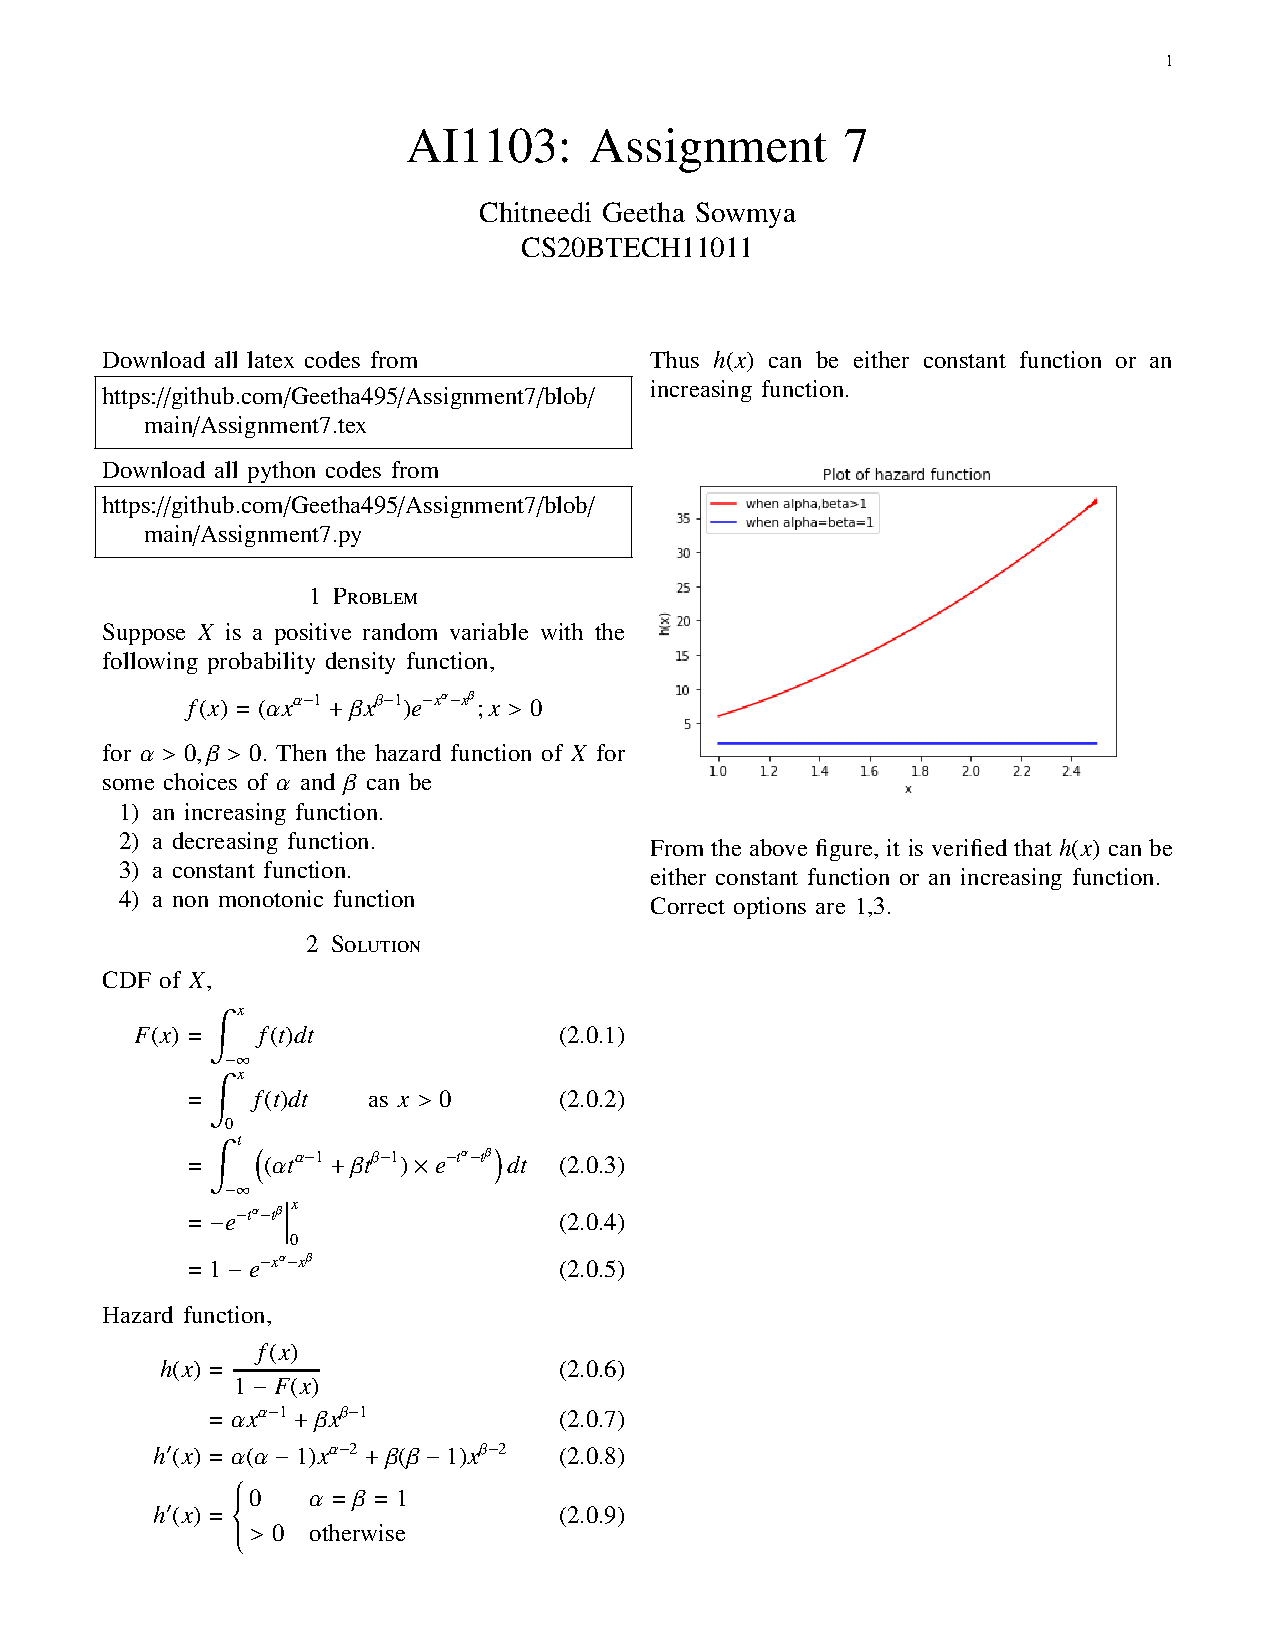
\includegraphics[width=\columnwidth]{Assignment7.png}
% \caption{pdf of $ Y=sign(X)$}
% \label{june/2012/112/pdf}
% \end{figure}
\begin{align}
   \implies \mu_y = 0 
\end{align}
and variance is
\begin{align}
    \sigma_y^2 &= (-1)^2\brak{\frac{1}{2}}+(1)^2\brak{\frac{1}{2}}\\
    &=1
\end{align}
\item Given
\begin{align}
    S_n&=\sum_{i=1}^{n} sign(X_i)\\
    S_n(\theta=0)&=\sum_{i=1}^{n} Y_i
\end{align}
From central limit theorem 
\begin{align}
    Z&=\lim_{n\to\infty}\sqrt{n}\brak{\frac{\frac{S_n}{n}-\mu_y}{\sigma_y}}\\
    &=\lim_{n\to\infty}\sqrt{n}\brak{\frac{S_n}{n}}\\
    &=\lim_{n\to\infty}\brak{\frac{S_n}{\sqrt{n}}}
    \label{june/2012/112/clt}
\end{align}
where Z is a standard normal variable N(0,1).
\begin{enumerate}
    \item Given
\begin{align}
    \alpha = P\cbrak{Z>z_\alpha}\label{june/2012/112/uff}
\end{align}
So from $\eqref{june/2012/112/clt}$ and $\eqref{june/2012/112/uff}$
\begin{align}
\lim_{n\to\infty}P\cbrak{\frac{S_n}{\sqrt{n}}>z_\alpha}&=
\alpha\\
\implies \lim_{n\to\infty}P\cbrak{S_n>\sqrt{n}z_\alpha}&=
\alpha
\end{align}
\end{enumerate}
\end{enumerate}
{$H_1:\theta >0$ is true}
\begin{enumerate}
    \item Given X is symmetric around $\theta>0$.Let us assume $\theta=\theta_0>0$.
    \begin{align}
        f_X(\theta_0-x)&=f_X(\theta_0+x)\\
        \int_{\theta_0}^{\infty} f_X(\theta_0-x)dx&=
        \int_{\theta_0}^{\infty} f_X(\theta_0+x)dx
        \label{june/2012/112/s}
    \end{align}
    \begin{enumerate}
        \item Solving LHS of $\eqref{june/2012/112/s}$.Changinng $(\theta_0-x) \rightarrow t$
        \begin{align}
           \int_{\theta_0}^{\infty} f_X(\theta_0-x)dx&=
           \int_{-\infty}^{0}f_X(t) dt\\
           &=\pr{X\leq0}\label{june/2012/112/temp}
        \end{align}
        \item Solving RHS of $\eqref{june/2012/112/s}$.Changing $(\theta_0+x) \rightarrow t$
        \begin{align}
           \int_{\theta_0}^{\infty} f_X(\theta_0+x)dx&=
           \int_{2\theta_0}^{\infty} f_X(t)dt\\
          &= \int_{0}^{\infty} f_X(t)dt-\int_{0}^{2\theta_0} f_X(t)dt\\
          &=\pr{X\geq0}-k\label{june/2012/112/u}
        \end{align}
        where
        \begin{align}
           k=\int_{0}^{2\theta_0} f_X(t)dt>0 
        \end{align}
    \end{enumerate}
    From $\eqref{june/2012/112/s}$,$\eqref{june/2012/112/t}$ and $\eqref{june/2012/112/u}$
    \begin{align}
        \pr{X\geq0}>\pr{X\leq0}
    \end{align}
    \item So
    \begin{align}
        \pr{Y=1}>\pr{Y=-1}
    \end{align}
    Therefore,if we perform the experiment and find the value of $\brak{\frac{S_n}{\sqrt{n}}}$,it is most likely to occur on the right side of the distribution of 
$\brak{\frac{S_n}{\sqrt{n}}}$.In $\eqref{june/2012/112/clt}$ it is shown that distrubution of the random variable $\brak{\frac{S_n}{\sqrt{n}}}$
 is $N(0,1)$ when n is very large.So
\begin{align}
    \lim_{n\to\infty}P\cbrak{\frac{S_n}{\sqrt{n}}>Z_\alpha}=1
\end{align}
\end{enumerate}
%
  

\end{enumerate}
% \section{Unsolved Problems}
% \renewcommand{\theequation}{\theenumi}
\renewcommand{\thefigure}{\theenumi}
\renewcommand{\thetable}{\theenumi}
\begin{enumerate}[label=\thesection.\arabic*.,ref=\thesection.\theenumi]
\numberwithin{equation}{enumi}
\numberwithin{figure}{enumi}
\numberwithin{table}{enumi}


\item Which of the following conditions imply independence of the random variables $X$
and $Y$ ?\\
\begin{enumerate}
    \item  $\pr{X\ \mathop{>}\ a|Y\ \mathop{>}\ a} = \pr{X\ \mathop{>}\ a}\ \forall\ a\ \in\ \mathbb{R}$\\ 
    \item  $\pr{X\ \mathop{>}\ a|Y\ \mathop{<}\ b} = \pr{X\ \mathop{>}\ a}\ \forall\ a,\ b\ \in\ \mathbb{R}$\\ 
    \item  $X$ and $Y$ are uncorrelated.\\
    \item  $E[(X-a)(Y-b)] = E(X-a)\ E(Y-b)\ \forall\ a,\ b \in\ \mathbb{R}$\\
\end{enumerate}

\end{enumerate}

%  \section{June 2019}
%  \renewcommand{\theequation}{\theenumi}
\renewcommand{\thefigure}{\theenumi}
\begin{enumerate}[label=\thesection.\arabic*.,ref=\thesection.\theenumi]
\numberwithin{equation}{enumi}
\numberwithin{figure}{enumi}



\item Consider a Markov Chain with state space $\cbrak{0,1,2}$ and transition matrix
\begin{align}
P = 
\begin{blockarray}{c@{\hspace{1pt}}rrr@{\hspace{3pt}}}
         & 0   & 1   & 2 \\
        \begin{block}{r@{\hspace{3pt}}@{\hspace{1pt}}
    (@{\hspace{1pt}}rrr@{\hspace{1pt}}@{\hspace{1pt}})}
        0 & \frac{1}{4} & \frac{5}{8} & \frac{1}{8}  \\[1mm]
        1 & \frac{1}{4} & 0 & \frac{3}{4}  \\[1mm]
        2 &  \frac{1}{2} & \frac{3}{8} & \frac{1}{8}  \\
        \end{block}
    \end{blockarray}
\end{align}
Then which of the following are true?
\begin{enumerate}
\item $\lim_{n \to \infty} p_{12}^{(n)} = 0$
\item $\lim_{n \to \infty} p_{12}^{(n)} = \lim_{n \to \infty} p_{21}^{(n)}$
\item $\lim_{n \to \infty} p_{22}^{(n)} = \frac{1}{8}$
\item $\lim_{n \to \infty} p_{21}^{(n)} = \frac{1}{3}$
\end{enumerate}
%
\item A sample of size $n =2$ is drawn from a population of size $N=4$ using probability proportional to size without replacement scheme , Where the probabilities proportional to size are
\begin{table}[h!]
\resizebox{\columnwidth}{0.6cm}{%
  \begin{tabular}{|c|c|c|c|c|}
    \hline
    i: & 1 & 2 & 3 & 4\\
    \hline
    $p_{i}$ & 0.4 & 0.2 & 0.2 & 0.2\\
    \hline
  \end{tabular}%
} 
   \caption*{Table : Probability vs Size}
\end{table}  
The probability of inclusion of unit (1) in the sample is 
\begin{enumerate}
\begin{multicols}{4}
\setlength\itemsep{2em}
\item $0.4$
\item $0.6$
\item $0.7$
\item $0.75$
\end{multicols}
%

\end{enumerate}
%
\solution
Let $P_{i}(j)$ represent the probability for selecting unit (j) as second unit after selecting  unit (i) 
\begin{align}
    P_{i}(j)&=\frac{p_{j}}{1-p_{i}}
    \label{2019-58:eq:eq2}
\end{align}
Let  $\pr{i,j}$ be probability of selecting sample \{i,j\} ,using \eqref{eq:eq2}  is 
\begin{align}
    \pr{i,j}&=P_{i}(j)+P_{j}(i)
    \\
    &=\brak{p_{i}\times \frac{p_{j}}{1-p_{i}}} + \brak{p_{j}\times \frac{p_{i}}{1-p_{j}}}
    \label{2019-58:eq:eq3}
\end{align}
Total samples(Size $n=2$)are 
\definecolor{green}{RGB}{0 150, 22}
\definecolor{Red}{RGB}{200,60,40}
\definecolor{mycolor}{RGB}{0, 60, 240}
\begin{table}[h!]
\resizebox{\columnwidth}{0.95cm}{%
  \begin{tabular}{|c ||c ||c |c | c| c| c|}
    \hline
    \textcolor{green}{Case }&  \textcolor{Red}{1} & \textcolor{Red}{2} & \textcolor{Red}{3} & \textcolor{Red}{4} & \textcolor{Red}{5} & \textcolor{Red}{6}\\
    \hline
    \textcolor{green}{Sample(size $n=2$)} & \textcolor{mycolor}{\brak{1,2}} & \textcolor{mycolor}{\brak{1,3} }& \textcolor{mycolor}{\brak{1,4} }& \textcolor{mycolor}{\brak{2,3}} & \textcolor{mycolor}{\brak{2,4}}& \textcolor{mycolor}{\brak{3,4}}\\
    \hline
  \end{tabular}%
} 
  \caption{ list of samples}
  \label{2019-58:tab:label1_test}
\end{table}
Let $P_{i}$ be the probability of inclusion of unit (i) in the sample(size $n=2$),Now i will calculate $P_{1}$ ,Favourable cases for inclusion of unit(1) are case (\textcolor{red}{1,2,3}),So
\begin{align}
    P_{1}&=\pr{1,2} +\pr{1,3}+\pr{1,4}
\end{align}
using \eqref{2019-58:eq:eq3} and $p_{i}$ from question ,
\begin{align}
    P_{1}&=\frac{7}{30} + \frac{7}{30} + \frac{7}{30}
    \\
    &=0.7
\end{align}
Therefore Option (3) is correct.

%
\item Consider the function \textit{f(x)} defined as \textit{f(x)} = \textit{ce$^{-x^{4}}$}, $\textit{x} \in R$ . For what value of \textit{c} is \textit{f} a probability density function?\\
\begin{enumerate}
    \item $\displaystyle\frac{2}{\Gamma(1/4)}$\\\label{june/2019/52/option 1}
    \item $\displaystyle\frac{4}{\Gamma(1/4)}$\\
    \item $\displaystyle\frac{3}{\Gamma(1/3)}$\\
    \item $\displaystyle\frac{1}{4\Gamma(4)}$
\end{enumerate}
%
\solution
Consider a continuous random variable X so that the function \textit{f} can be probability density function if and only if it satisfies the condition 
\begin{align}
    \int_{-\infty}^{\infty}f_{X}(u)du = 1 \label{2019/52/equation 1}
\end{align}
Hence by applying the \eqref{2019/52/equation 1} for the function \textit{f} we get
\begin{align}
    \int_{-\infty}^{\infty}ce^{-u^{4}}du = 1\\
    2c\int_{0}^{\infty}e^{-u^{4}}du = 1\label{2019/52/equation 2}\\
    2c\int_{0}^{\infty}e^{-t}\frac{dt}{4t^{\frac{3}{4}}} = 1\\
    \frac{c}{2}\int_{0}^{\infty}e^{-t}t^{-\frac{3}{4}}dt = 1\label{2019/52/equation 3}
\end{align}
We know that gamma function for any real positive $\alpha$
\begin{align}
    \Gamma(\alpha) = \int_0^\infty x^{\alpha - 1} e^{-x} dx \label{2019/52/gammafunction}
\end{align}
Hence by using \eqref{2019/52/gammafunction} in \eqref{2019/52/equation 3} we get
\begin{align}
    \frac{c}{2}\Gamma(1/4) = 1\\
    c=\frac{2}{\Gamma(1/4)}
\end{align}
Hence $c = \displaystyle\frac{2}{\Gamma(1/4)}$ and option \eqref{2019/52/option 1} is correct.\newline\newline
The CDF of \textit{f} by using \eqref{2019/52/gammafunction} we get
\begin{align}
    F_{X}(x) &= \int_{0}^{x}f(u)du\\
             &= \frac{2}{\Gamma(\frac{1}{4})}\int_{0}^{x}e^{-u^{4}}du\\
             &= \frac{2}{4\Gamma(\frac{1}{4})}\int_{0}^{x^{4}}e^{-t}{t^{\frac{-3}{4}}}dt\\
             &= \frac{1}{2\Gamma(\frac{1}{4})}\int_{0}^{x^{4}}e^{-t}{t^{\frac{-3}{4}}}dt\\
             &= \frac{1}{2\Gamma(\frac{1}{4})}\brak{\Gamma\brak{\frac{1}{4}}-\Gamma\brak{\frac{1}{4},x^{4}}}\\
             &= \frac{1}{2\Gamma(\frac{1}{4})}\gamma\brak{\frac{1}{4},x^{4}}
\end{align}
%
\item Consider a simple symmetric random walk on integers ,Where from every state i you to move to i-1 and i+1 with  probability half each. Then which of the following are correct?
\begin{enumerate}
    \item The random walk is aperiodic
    \item The random walk is irreducible
    \item The random walk is null recurrent 
    \item The random walk is positive recurrent 
\end{enumerate}
%
\solution
This is a Markov Chain ,Where the state space consists of the integers $(i=0,\pm1,\pm2,\pm3,...)$ and transition  probability is given as
\begin{align}
   P_{i,i+1} &= p =\frac{1}{2}
   \\
   P_{i,i-1} & =q =\frac{1}{2}
\end{align}
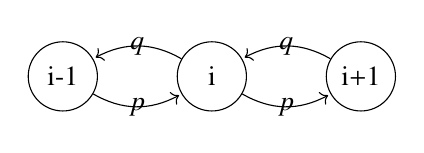
\begin{tikzpicture}
    
    \node[state]  (p) {i-1};
    \node[state,right=of p]  (q) {i};
    \node[state,right=of q]  (r) {i+1};
    \draw[every loop]
    (p) edge[bend right] node {$p $} (q)
    (q) edge[bend right] node {$q $} (p)
    (q) edge[bend right] node {$p$} (r)
    (r) edge[bend right] node {$q $} (q);
   
\end{tikzpicture}
Let $P_{i,j}^{n}$ denotes the probability of being in state j after nth transition starting from state i.
\begin{enumerate}
    \item We know that for state j in Markov chain to be \textbf{aperiodic} ,Then their  exist k such that $P_{j,j}^{n} > 0$ for all $n \geq k$. but for to return to same state j after n transitions  ,Number of forward steps should be equal to Backward steps , i.e for odd n in (2m +1)form
    \begin{align}
        P_{j,j}^{2m+1}&=0  
        \label{2019/105/eq:eq1}
    \end{align}
    when n is even in 2m form
    \begin{align}
        P_{j,j}^{2m}&=\binom{2m}{m}p^{m}q^{m}
     \\
     &=\frac{(2m)!}{m!.m!}p^{m}q^{m}
     \label{2019/105/eq:eq2}
    \end{align}
    ,As for odd n $P_{j,j}^{n} = 0$ ,$P_{j,j}^{n} > 0$ for all $n \geq k$ is not possible .which implies  all states are \textbf{Periodic}
  
    Option (1) is \textbf{incorrect}. 
    \item 
In a Markov Chain for state j to be recurrent then it should satisfy following condition
\begin{align}
     \lim_{t\to\infty}\sum_{n=1}^t P_{j,j}^{n}&=\infty
\end{align}
using Stirling approximation in equation \eqref{2019/105/eq:eq2} 
\begin{align}
    P_{j,j}^{2m} &=\frac{((2m)^{2m +\frac{1}{2}}).e^{-2m}.(2\pi)^{\frac{1}{2}}}{m^{m+\frac{1}{2}}.e^{-m}.m^{m+\frac{1}{2}}.e^{-m}.2\pi}.p^{m}q^{m}
    \\
    &=\frac{(4pq)^{2m}}{(m\pi)^{\frac{1}{2}}}
    \label{2019/105/eq:eq3}
\end{align}
In this question $p =\frac{1}{2}=q$,then using \eqref{2019/105/eq:eq1} and \eqref{2019/105/eq:eq3}
\begin{align}
    \lim_{t\to\infty}\sum_{n=1}^t P_{j,j}^{n}&=\sum_{n=2k,k=1}^{\infty}\frac{1}{(\frac{n}{2}\pi)^{\frac{1}{2}}}
\end{align}
Since $\frac{1}{n^{\frac{1}{2}}}$ is divergent,
\begin{align}
     \lim_{t\to\infty}\sum_{n=1}^t P_{j,j}^{n}& = \infty
\end{align}
Therefore state j is recurrent ,as what we calculated is independent of j ,all states are \textbf{recurrent }.
The first-passage-time probability, $f_{i,j}(n)$, of a Markov chain is the probability,given as 
\begin{equation}
\resizebox{.9\hsize}{!}{$f_{i,j}(n)=\pr{X_{n}=j,X_{n-1}\neq j,X_{n-2}\neq j,\dots X_{1}\neq j|X_{0}=i}$}
\end{equation}
The first-passage time $T_{j,j}$from a state j back to itself is of particular importance. It has the PMF $f_{j,j}(n)$ amd Distribution function $F_{j,j}(n)$
\begin{align}
    F_{j,j}(n)&=\sum_{k=0}^n f_{j,j}(k)
    \label{2019/105/eq:eq4}
\end{align}
We Know that all states are recurrent .Now i will find whether they are null recurrent or positive recurrent .
For positive recurrent 
\begin{align}
    \overline{T_{j,j}}& < \infty
\end{align}
For null recurrent 
\begin{align}
    \overline{T_{j,j}}& = \infty
\end{align}
Where $\overline{T_{j,j}}$ is mean time to enter state j starting from j.
Now calculating $\overline{T_{j,j}}$ using below formula,
\begin{align}
    \overline{T_{j,j}}&=1 + \sum _{k=0}^n (1 - F_{j,j}(k))
    \label{2019/105/eq:eq5}
\end{align}
Using \eqref{2019/105/eq:eq5} and \eqref{2019/105/eq:eq4},We get 
\begin{align}
    \overline{T_{j,j}}& = \infty
\end{align}
Therefore all states are null recurrent.
Option(3) is \textbf{correct}
 \item
    Since all states are recurrent,they communicate with each other ,therefore Markov chain is irreducible , option (2) is \textbf{correct}
 \item As all states are null recurrent , option (4) is \textbf{incorrect} 
\end{enumerate}
Therefore correct options are \textbf{2,3}


\end{enumerate}


% \section{December 2018}
% \renewcommand{\theequation}{\theenumi}
\renewcommand{\thefigure}{\theenumi}
\begin{enumerate}[label=\thesection.\arabic*.,ref=\thesection.\theenumi]
\numberwithin{equation}{enumi}
\numberwithin{figure}{enumi}
\numberwithin{table}{enumi}

\item Let X and Y be i.i.d random variables uniformly distributed on (0,4).Then \pr{X>Y|X<2Y} is
\begin{enumerate}
    \item 1/3
    \item 5/6
    \item 1/4
    \item 2/3
\end{enumerate}
\solution

The PDF is given by
\begin{align}
   &f_X (x)=f_Y (x)=\nonumber \begin{cases}
         \frac{1}{4}, &\text{if 0 \(< x <\) 4}\\
         0, &\text{otherwise}\\
   \end{cases} 
\end{align}    
The CDF is given by
\begin{align}
   \nonumber& F(x)=\int_{-\infty}^{x} f(x)dx \\ \nonumber
   &F_X (x)=F_Y (x)=\nonumber \begin{cases}
          0, & x\leq 0\\
         \frac{x}{4}, &\text{if 0 \(< x <\) 4}\\
          1, &x\geq4\\
   \end{cases}    
\end{align}
Using definition of conditional probability 
\begin{align}
    &\pr{X>Y|X<2Y}=\frac{\pr{Y < X< 2Y}}{\pr{X<2Y}} \label{eqn1}
\end{align}
Now finding \pr{X<2Y}
\begin{align}
    &\pr{X<2y}=F_X (2y)\\
    \implies& \pr{X<2Y}=\int_{-\infty}^{\infty} f_Y(x) \times F_X (2x)dx\\
    \implies& \pr{X<2Y}=\int_{0}^{2} \frac{x}{8}dx +\int_{2}^{4}\frac{1}{4}dx\\
    \implies& \pr{X<2Y}=\frac{3}{4}=0.75 \label{eqn2}
\end{align}
Now to find \pr{Y<X<2Y}
\begin{align}
    &\pr{y<X<2y}=F_X (2y)- F_X (y) \\
    \implies &\pr{Y<X<2Y}\\ \nonumber 
    &=\int_{-\infty}^{\infty} f_Y (x)( F_X (2x)- F_X(x))dx \\
   \implies &\int_{0}^{2}\frac{1}{4}\brak{\frac{x}{2}-\frac{x}{4}} dx +\int_{2}^{4}\frac{1}{4}\brak{1-\frac{x}{4}} dx\\
   \implies &\pr{Y<X<2Y}=\frac{1}{4}=0.25 \label{eqn3}
\end{align}
Now using \eqref{eqn1},\eqref{eqn2} and \eqref{eqn3}
\begin{align}
    \pr{X>Y|X<2Y}=\frac{1/4}{3/4}=\frac{1}{3}
\end{align}
Hence final solution is option 1) or 1/3 
%
\item Suppose $X$ is a positive random variable with the following probability density function,
\begin{align*}
f(x) = (\alpha x^{\alpha -1} + \beta x^{\beta-1} ) e^{-x^{\alpha}-x^{\beta}} ; x>0
\end{align*}
for $ \alpha >0, \beta >0$.
Then the hazard function of $X$ for some choices of $\alpha$ and $\beta$ can be
\begin{enumerate}
    \item an increasing function.
    \item a decreasing function.
    \item a constant function.
    \item a non monotonic function
\end{enumerate}
%
\solution


CDF of $X$, 
\begin{align}
    F(x) &=  \int_{-\infty}^xf(t)dt \\
    &= \int_{0}^xf(t)dt \hspace{1cm} \text{as } x>0\\
    &= \int_{-\infty}^t\left((\alpha t^{\alpha -1} + \beta t^{\beta-1} ) \times e^{-t^{\alpha}-t^{\beta}}\right)dt \\
    &= -e^{-t^{\alpha}-t^{\beta}} \Big|_0^x\\
    &= 1-e^{-x^{\alpha}-x^{\beta}}
\end{align}
Hazard function,
\begin{align}
    h(x) &= \frac{f(x)}{1-F(x)} \\
    &= \alpha x^{\alpha -1} + \beta x^{\beta-1} \\
    h^{\prime}(x) &= \alpha(\alpha -1) x^{\alpha -2} + \beta(\beta-1) x^{\beta-2}\\
     h^{\prime}(x) &= 
         \begin{cases}
    0 & \alpha=\beta=1 \\
    >0 & \text{otherwise}\\
    \end{cases}
    \end{align}
    Thus $h(x)$ can be either constant function or an increasing function.
    
    \begin{figure}[h]
    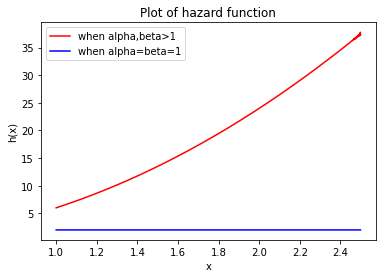
\includegraphics[width=\columnwidth]{solutions/2018/dec/118/figures/plot.png}
    \end{figure}
     From the above figure, it is verified that $h(x)$ can be either constant function or an increasing function.\\
       Correct options are 1,3.





%
\item Suppose n units are drawn from a population of N units sequentially as follows. A random sample
\begin{align}
    U_1, U_2, ... U_N \text{ of size N, drawn from }U\brak{0, 1} 
\end{align} 
The k-th population unit is selected if 
\begin{align}
    U_k<\frac{n - n_k}{N-k+1}, k = 1, 2, ..N. \text{where, } n_1=0, n_k = 
\end{align}
number of units selected out of first k-1 units for each k = 2, 3, ..N. Then,
\begin{enumerate}
    \item The probability of inclusion of the second unit in the sample
    \begin{align}
        \text{ is } \frac{n}{N}
    \end{align}
    \item The probability of inclusion of the first and the second unit in the sample
    \begin{align}
        \text{ is } \frac{n \brak{n-1}}{N \brak{N-1}}
    \end{align}
    \item The probability of not including the first and including the second unit in the sample
    \begin{align}
        \text{ is } \frac{n \brak{N-n}}{N \brak{N-1}}
    \end{align}
    \item The probability of including the first and not including the second unit in the sample
    \begin{align}
        \text{ is } \frac{n \brak{n-1}}{N \brak{N-1}}
    \end{align}
\end{enumerate}
%
\solution
\input{solutions/2018/dec/116.tex}
%
\item Consider a Markov chain with state space {1,2,....,100}. Suppose states 2i and 2j communicate with each other and states 2i-1 and 2j-1 communicate with each other for every i,j = 1,2,...,50. Further suppose that $p^{(2)}_{3,3}$ > 0,$p^{(3)}_{4,4}$ > 0 and $p^{(7)}_{2,5}$ > 0. Then 
\begin{enumerate}
\item The Markov chain is irreducible.
\item The Markov chain is aperiodic.
\item State 8 is recurrent.
\item State 9 is recurrent.
\end{enumerate}
%
\solution
\input{solutions/2014/dec/106/LaTex/Assignment_7.tex}
%
\item 


% \item Consider a Markov Chain with state space $\cbrak{0,1,2}$ and transition matrix
% \begin{align}
% P = 
% \begin{blockarray}{c@{\hspace{1pt}}rrr@{\hspace{3pt}}}
%          & 0   & 1   & 2 \\
%         \begin{block}{r@{\hspace{3pt}}@{\hspace{1pt}}
%     (@{\hspace{1pt}}rrr@{\hspace{1pt}}@{\hspace{1pt}})}
%         0 & \frac{1}{2} & \frac{1}{2} & 0  \\
%         1 & 0 &\frac{1}{2}  & \frac{3}{4}  \\
% %
%         2 &  \frac{1}{3} & \frac{1}{3} & \frac{1}{3}  \\
%         \end{block}
%     \end{blockarray}
% \end{align}
% For any two states $i$ and $j$, let $p_{ij}^{(n)}$ denote the $n$-step transition probability of going from $i$ to $j$.  Identify correct statements.
% \begin{enumerate}
% \item $\lim_{n \to \infty} p_{11}^{(n)} = \frac{2}{9}$
% \item $\lim_{n \to \infty} p_{21}^{(n)} = 0$
% \item $\lim_{n \to \infty} p_{32}^{(n)} = \frac{1}{3}$
% \item $\lim_{n \to \infty} p_{13}^{(n)} = \frac{1}{3}$
% \end{enumerate}
% \solution
% See Tables \ref{eq:solutions/2018/dec/106/table0} and \ref{eq:solutions/2018/dec/106/table1}


\onecolumn
	\begin{longtable}{|l|l|}
		\hline
		\multirow{3}{*}{Irreducible Markov Chain} 
		& \\
		& A Markov chain is $\textbf{irreducible}$ if all the states communicate with each other,\\
		& i.e., if there is only one communication class.\\
		&\\
		\hline
		\multirow{3}{*}{Aperiodic Markov Chain} & \\
		& If there is a self-transition in the chain ($p^{ii}>0$ for some i), then the chain is\\
		& called as $\textbf{aperiodic}$\\
		& \\
		\hline
		\multirow{3}{*}{Stationary Distribution} & \\
		& A stationary distribution of a Markov chain is a probability distribution that\\
		& remains unchanged in the Markov chain as time progresses. Typically, it is\\
		& represented as a row vector $\Vec{\pi}$ whose entries are probabilities summing to 1,\\ 
		& and given transition matrix $\textbf{P}$, it satisfies\\
		& \\
		&  \qquad \qquad  \qquad$\Vec{\pi} = \Vec{\pi} \textbf{P}$\\
		& \\
		\hline
\caption{}
\label{eq:solutions/2018/dec/106/table0}
	\end{longtable}
	\begin{longtable}{|l|l|}
		\hline
		\multirow{3}{*}{Drawing Transition diagram} 
		& \\
		& 
		
		$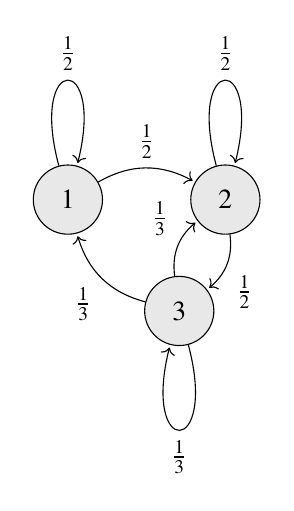
\begin{tikzpicture}[shorten >=1pt,node distance=2cm, scale =3, auto]
			\tikzstyle{every state}=[fill={rgb:black,1;white,10}]
			
			\node[state]   (q_1)                          {$1$};
			\node[state]   (q_2)  [right of=q_1]          {$2$};
			\node[state]   (q_3)  [below right of=q_1]          {$3$};
			
			\path[->]
			(q_1) edge [loop above] node {$\frac{1}{2}$}    (   )
			edge [bend left]  node {$\frac{1}{2}$}    (q_2)
			(q_2) edge [bend left]  node {$\frac{1}{2}$}    (q_3)
			edge [loop above] node {$\frac{1}{2}$}    ()
			(q_3) edge [bend left]  node {$\frac{1}{3}$}    (q_2)
			edge [bend left]  node {$\frac{1}{3}$}    (q_1)
			edge [loop below] node {$\frac{1}{3}$}    ();
		\end{tikzpicture}$
		
		\\  
		&\\
		&\\
		\hline
		\multirow{3}{*}{Checking whether the  } & \\
		& Here,\\chain is Irreducible
		& All the states are accessible to one another. \\and Aperiodic
		& $\implies$ They are in the same communication class. So, it is Irreducible.\\
		& \\
		& There exists the non- zero self-transition, which means that the chain \\
		& is Aperiodic.\\
		&\\ 
		& We know that if the Markov Chain is irreducible and aperiodic then \\
		& \qquad \qquad \qquad $\Vec{\pi}_{j} = \lim_{n \to \infty}P\{X_{n} = j\}$, $j = 1,...,N$ \\
		& These are the stationary probabilities. \\
		&\\
		\hline
		\multirow{3}{*}{Finding the Stationary} & \\
		& Stationary Probability can be represented as\\Probability Distributions
		& \qquad \qquad \qquad $\Vec{\pi} = \Vec{\pi} \vec{P}$\\
		& \\
		& \qquad $\implies$ $\myvec{v_{1}&&v_{2}&&v_{3}} = \myvec{v_{1}&&v_{2}&&v_{3}}\vec{P}$ \\
		& \\
		& Equating the above equation we get \\
		& \\
		& \qquad \qquad \qquad $\frac{1}{2}v_{1}-\frac{1}{3}v_{3} = 0$ $\label{eq:solutions/2018/dec/106/eq}$\\
		& \\
		& \qquad \qquad \qquad $\frac{1}{2}v_{1}-\frac{1}{2}v_{2} + \frac{1}{3}v_{3} = 0$\\
		& \\
		& \qquad \qquad \qquad $\frac{1}{2}v_{2}-\frac{2}{3}v_{3} = 0$\\
		& \\\
		& We see that summation of second and the third equation gives us the \\
		& first equation only. \\
		& And we know that the probability distribution will sum up to 1. \\
		& \\
		& \qquad \qquad \qquad $v_{1}+v_{2}+v_{3} = 1$ \\
		& \\
		& Therefore, we get the equation form as \\
		& \\
		& \qquad \qquad \qquad $\myvec{1&1&1\\\frac{1}{2}&0&\frac{-1}{3}\\\frac{1}{2}&\frac{-1}{2}&\frac{1}{3}}\myvec{v_{1}\\v_{2}\\v_{3}} = \myvec{1\\0\\0}$ \\
		& \\
		\hline
		\multirow{3}{*}{Solving the linear} & \\
		& The above linear equation can be solved using Gauss-Jordan method as\\equtions
		& \\
		& \qquad \qquad \qquad $\myvec{1&1&1&\vrule&1\\\frac{1}{2}&0&\frac{-1}{3}&\vrule&0\\\frac{1}{2}&\frac{-1}{2}&\frac{1}{3}&\vrule&0}$\\
		& \\
		& \qquad $\xleftrightarrow[]{R_2 \leftarrow R_2 - \frac{1}{2}R_1}$
		$\myvec{1&1&1&\vrule&1\\0&\frac{-1}{2}&\frac{-5}{6}&\vrule&\frac{-1}{2}\\\frac{1}{2}&\frac{-1}{2}&\frac{1}{3}&\vrule&0}$\\
		&\\
		& \qquad $\xleftrightarrow[]{R_3 \leftarrow R_3 - \frac{1}{2}R_1}$
		$\myvec{1&1&1&\vrule&1\\0&\frac{-1}{2}&\frac{-5}{6}&\vrule&\frac{-1}{2}\\0&-1&\frac{-1}{6}&\vrule&\frac{-1}{2}}$\\
		&\\
		& \qquad $\xleftrightarrow[]{R_2 \leftarrow \frac{-1}{2}R_2}$
		$\myvec{1&1&1&\vrule&1\\0&1&\frac{5}{3}&\vrule&1\\0&-1&\frac{-1}{6}&\vrule&\frac{-1}{2}}$\\
		&\\
		& \qquad $\xleftrightarrow[]{R_3 \leftarrow R_3 + R_2}$
		$\myvec{1&1&1&\vrule&1\\0&1&\frac{5}{3}&\vrule&1\\0&0&\frac{3}{2}&\vrule&\frac{1}{2}}$\\
		&\\
		& \qquad $\xleftrightarrow[]{R_3 \leftarrow \frac{3}{2}R_3}$
		$\myvec{1&1&1&\vrule&1\\0&1&\frac{5}{3}&\vrule&1\\0&0&1&\vrule&\frac{1}{3}}$\\
		&\\
		& \qquad $\xleftrightarrow[]{R_2 \leftarrow R_2 - \frac{5}{3}R_3}$
		$\myvec{1&1&1&\vrule&1\\0&1&0&\vrule&\frac{4}{9}\\0&0&1&\vrule&\frac{1}{3}}$\\
		&\\
		& \qquad $\xleftrightarrow[]{R_1 \leftarrow R_1 - R_3}$
		$\myvec{1&1&0&\vrule&\frac{2}{3}\\0&1&0&\vrule&\frac{4}{9}\\0&0&1&\vrule&\frac{1}{3}}$\\
		&\\
		& \qquad $\xleftrightarrow[]{R_1 \leftarrow R_1 - R_2}$
		$\myvec{1&0&0&\vrule&\frac{2}{9}\\0&1&0&\vrule&\frac{4}{9}\\0&0&1&\vrule&\frac{1}{3}}$\\
		&\\
		& $\therefore$, stationary probability distribution $\pi$ is given by \\
		& \qquad \qquad $\pi = \myvec{\frac{2}{9} & \frac{4}{9} & \frac{1}{3}}$ \\
		& \\
		\hline
		\multirow{3}{*}{Observations} & \\
		
		
		& Since the given transition probability matrix $\vec{P}$ is irreducible and aperiodic, \\
		& then $\lim_{n \to \infty} \vec{P}^{n}$ converges to a matrix with all rows identical and equal to $\vec{\pi}$. \\
		& \\
		& We were able to find $\vec{\pi}$ as $\myvec{\frac{2}{9} & \frac{4}{9} & \frac{1}{3}}$ \\
		& \\
		& $\lim_{n \to \infty} \vec{P}^{n} = \myvec{\frac{2}{9}&\frac{4}{9}&\frac{1}{3}\\\frac{2}{9}&\frac{4}{9}&\frac{1}{3}\\\frac{2}{9}&\frac{4}{9}&\frac{1}{3}}$\\
		& \\
		& From the above matrix, we get \\
		& \\
		& $\lim_{n \to \infty} \vec{P}^{n}_{11} = \frac{2}{9}$ \\
		&\\
		& $\lim_{n \to \infty} \vec{P}^{n}_{21} = \frac{2}{9}$ \\
		&\\
		& $\lim_{n \to \infty} \vec{P}^{n}_{32} = \frac{4}{9}$ \\
		&\\
		& $\lim_{n \to \infty} \vec{P}^{n}_{13} = \frac{1}{3}$ \\
		&\\
		\hline
		\multirow{3}{*}{Conclusion} & \\
		& From our observation we see that \\
		&\\
		& Options 1) and 4) are True.\\
		& \\
		\hline
\caption{}
\label{eq:solutions/2018/dec/106/table1}
	\end{longtable}
\twocolumn


\end{enumerate}

% \section{June 2018}
% \renewcommand{\theequation}{\theenumi}
\renewcommand{\thefigure}{\theenumi}
\begin{enumerate}[label=\thesection.\arabic*.,ref=\thesection.\theenumi]
\numberwithin{equation}{enumi}
\numberwithin{figure}{enumi}

\item Two students are solving the same problem independently,if the probability of first one solves the problem is $\frac{3}{5}$ and the probability that the second one solves the problem is $\frac{4}{5}$ ,what is the probability that atleast one of them solves the problem?
\begin{enumerate}

\item $ \frac{17}{25}$\\
\item $\frac{19}{25}$\\
\item $ \frac{21}{25}$\\
\item $\frac{23}{25}$

\end{enumerate}
%
\solution
Let X,Y be two events representing solving the problem by students A,B respectively.\\
Given 
\begin{align}
    \pr{X}=\frac{3}{5}\label{june2018-18:eq:0.0.1}\\
    \pr{Y}=\frac{4}{5}\label{june2018-18:eq:0.0.2}
\end{align}
Since students solve the problem independently,So events X and Y are independent,
For independent events
\begin{align}
    \pr{XY}&=\pr{X}\times \pr{Y}
\intertext{from \eqref{june2018-18:eq:0.0.1} and \eqref{june2018-18:eq:0.0.2}}
    \pr{XY}&=\frac{3}{5}\times \frac{4}{5}\\
    \pr{XY}&=\frac{12}{25}\label{june2018-18:eq:0.0.5}
\end{align}
\\
\\Now we have to find probability of solving the problem by atleast one of them i.e $\pr{X+Y}$.\\
As,
\begin{align}
    \pr{X+Y}&=\pr{X}+\pr{Y}-\pr{XY}\\
\intertext{from \eqref{june2018-18:eq:0.0.1}, \eqref{june2018-18:eq:0.0.2}, \eqref{june2018-18:eq:0.0.5}}
\pr{X+Y}&=\frac{3}{5}+\frac{4}{5}-\frac{12}{25}\\
\pr{X+Y}&=\frac{23}{25}
\end{align}
Hence the required probability is $\frac{23}{25}$
%
\item A standard fair die is rolled until some face other than 5 or 6 turns up.Let X denote the face value of the last roll.Let A=\{X is even\} and B=\{X is atmost 2\}
Then,
\begin{enumerate}
\begin{multicols}{2}
\setlength\itemsep{1em}
\item $\Pr{(A\cap {B})}=0$\\
\item $\Pr{(A \cap B)}=\frac{1}{6}$\\
\item $\Pr{(A\cap B)}=\frac{1}{4}$\\
\item $\Pr{({A} \cap {B})}=\frac{1}{3}$
\end{multicols}
\end{enumerate}
%
\solution
\begin{figure}[h!]
    \caption{Markov chain}
    \resizebox{\columnwidth}{!}{%
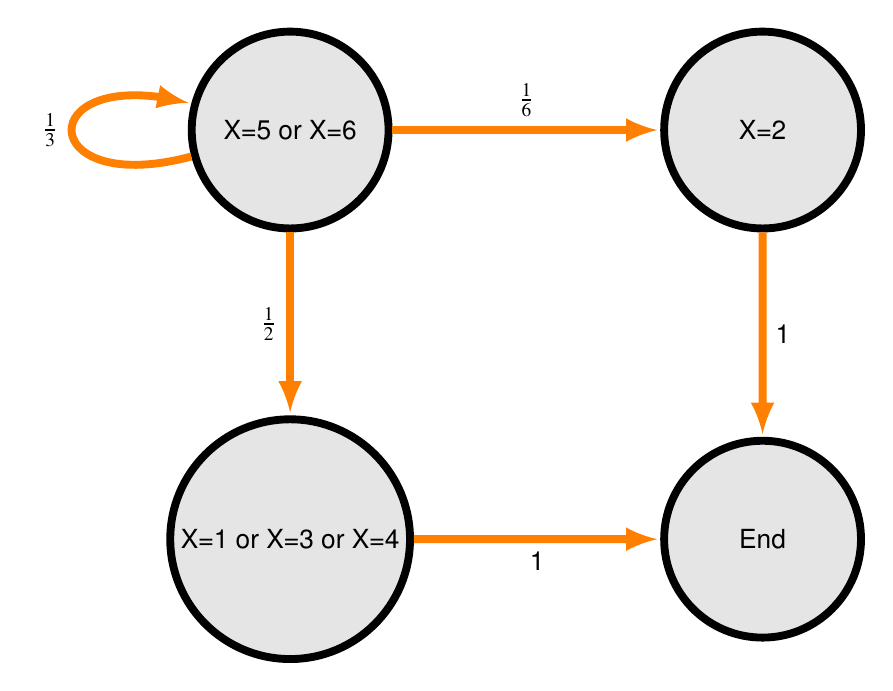
\begin{tikzpicture}[font=\sffamily]
        % Setup the style for the states
        \tikzset{node style/.style={state, 
                                    minimum width=2.5cm,
                                    line width=1mm,
                                    fill=gray!20!white}}
        % Draw the states
        \node[node style] at (0, 0)     (A)     {X=5 or X=6};
        \node[node style] at (6, 0)     (B)     {X=2};
        \node[node style] at (6, -5.196) (end) {End};
        \node[node style] at (0, -5.196) (C) {X=1 or X=3 or X=4};
        % Connect the states with arrows
        \draw[every loop,
              auto=right,
              line width=1mm,
              >=latex,
              draw=orange,
              fill=orange]
              (A) edge[bend left=0] node {$\frac{1}{2}$} (C)
              (C) edge[bend left=0] node {1} (end)
              (A) edge[loop left] node {$\frac{1}{3}$} (A)
            (A)     edge[bend right=0, auto=left] node {$\frac{1}{6}$} (B)
            (B)     edge[bend left=0, auto=left] node {1} (end);
    \end{tikzpicture}
    }
    \end{figure}
Let us assume the following table.
\begin{table}[h!]
\centering
\caption{}
\label{june2018-49:table:1}
\resizebox{\columnwidth}{!}{%
\begin{tabular}{|c|c|c|c|}
    \hline
    state 1&state 2 &state 3 &state 4\\
    \hline
$X=5$ or $X=6$&$X=2$&$X=1$ or $X=3$ or $X=4$ &end \\    
    \hline
\end{tabular}}
\end{table}
Let us represent the markov chain diagram in a matrix.Let $P_{ij}$ represent the element of a matrix which is in $i^{th}$ row and $j^{th}$ column.The value of $P_{ij}$ is equal to probability of transition from state $i$ to state $j$
\begin{equation}
P=\begin{bmatrix}
\frac{1}{3}&\frac{1}{6}&\frac{1}{2}&0\\
0&0&0&1\\
0&0&0&1\\
0&0&0&0\\
\end{bmatrix}
\end{equation}
We need the probability that $X=2$.Hence required probability is
\begin{equation}
    P_{12}+(P_{12})^{2}+\cdots+\infty \label{june2018-49:eq:reqprob}
\end{equation}
where $P_{12}^{n}$ represents the 1st row ,2nd column element in the $P^{n}$
\begin{align}
P^2&=\begin{bmatrix}
\frac{1}{3}&\frac{1}{6}&\frac{1}{2}&0\\
0&0&0&1\\
0&0&0&1\\
0&0&0&0\\
\end{bmatrix} \times
\begin{bmatrix}
\frac{1}{3}&\frac{1}{6}&\frac{1}{2}&0\\
0&0&0&1\\
0&0&0&1\\
0&0&0&0\\
\end{bmatrix}\\
&=\begin{bmatrix}
\frac{1}{9}&\frac{1}{18}&\frac{1}{6}&0\\
0&0&0&0\\
0&0&0&0\\
0&0&0&0\\
\end{bmatrix}
\end{align}
\begin{align}
    P^3&=(P^2)(P^1)\\
    &=\begin{bmatrix}
\frac{1}{9}&\frac{1}{18}&\frac{1}{6}&0\\
0&0&0&0\\
0&0&0&0\\
0&0&0&0\\
\end{bmatrix}\times
\begin{bmatrix}
\frac{1}{3}&\frac{1}{6}&\frac{1}{2}&0\\
0&0&0&1\\
0&0&0&1\\
0&0&0&0\\
\end{bmatrix}\\
&=\begin{bmatrix}
\frac{1}{27}&\frac{1}{54}&\frac{1}{18}&0\\
0&0&0&0\\
0&0&0&0\\
0&0&0&0\\
\end{bmatrix}
\end{align}
From above we can notice that each time $P_{12}$ reduces by $\frac{1}{3}$.Hence from \eqref{june2018-49:eq:reqprob},
\begin{equation}
    \sum_{i=0}^{\infty}\brak{\frac{1}{3}}^i \frac{1}{6}
\end{equation}
From Geometric progression we can write ,required probability =$\frac{1}{4}$
$\therefore$ \textbf{option C is correct}
%
\item Let X and Y be two random variables with joint probability density function
\begin{align*}
    f(x.y)=
    \begin{cases}
    \cfrac{1}{\pi} & 0\le x^2 + y^2 \le 1\\
    0 & otherwise
    \end{cases}
\end{align*}
Which of the following statements are correct?
\begin{enumerate}
    \item
    X and Y are independent.
    
    \item
    $\pr{X>0}=\cfrac{1}{2}$
    
    \item
    E(Y)=0
    
    \item
    Cov(X,Y)=0
\end{enumerate}
%
%
\solution
%\begin{figure}[h!]
    \caption{Markov chain}
    \resizebox{\columnwidth}{!}{%
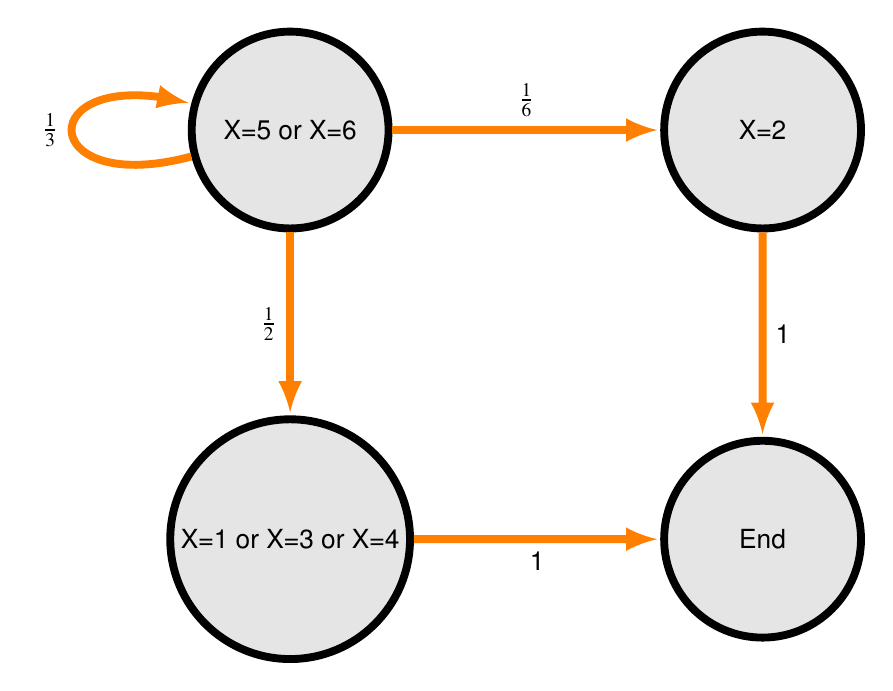
\begin{tikzpicture}[font=\sffamily]
        % Setup the style for the states
        \tikzset{node style/.style={state, 
                                    minimum width=2.5cm,
                                    line width=1mm,
                                    fill=gray!20!white}}
        % Draw the states
        \node[node style] at (0, 0)     (A)     {X=5 or X=6};
        \node[node style] at (6, 0)     (B)     {X=2};
        \node[node style] at (6, -5.196) (end) {End};
        \node[node style] at (0, -5.196) (C) {X=1 or X=3 or X=4};
        % Connect the states with arrows
        \draw[every loop,
              auto=right,
              line width=1mm,
              >=latex,
              draw=orange,
              fill=orange]
              (A) edge[bend left=0] node {$\frac{1}{2}$} (C)
              (C) edge[bend left=0] node {1} (end)
              (A) edge[loop left] node {$\frac{1}{3}$} (A)
            (A)     edge[bend right=0, auto=left] node {$\frac{1}{6}$} (B)
            (B)     edge[bend left=0, auto=left] node {1} (end);
    \end{tikzpicture}
    }
    \end{figure}
Let us assume the following table.
\begin{table}[h!]
\centering
\caption{}
\label{june2018-49:table:1}
\resizebox{\columnwidth}{!}{%
\begin{tabular}{|c|c|c|c|}
    \hline
    state 1&state 2 &state 3 &state 4\\
    \hline
$X=5$ or $X=6$&$X=2$&$X=1$ or $X=3$ or $X=4$ &end \\    
    \hline
\end{tabular}}
\end{table}
Let us represent the markov chain diagram in a matrix.Let $P_{ij}$ represent the element of a matrix which is in $i^{th}$ row and $j^{th}$ column.The value of $P_{ij}$ is equal to probability of transition from state $i$ to state $j$
\begin{equation}
P=\begin{bmatrix}
\frac{1}{3}&\frac{1}{6}&\frac{1}{2}&0\\
0&0&0&1\\
0&0&0&1\\
0&0&0&0\\
\end{bmatrix}
\end{equation}
We need the probability that $X=2$.Hence required probability is
\begin{equation}
    P_{12}+(P_{12})^{2}+\cdots+\infty \label{june2018-49:eq:reqprob}
\end{equation}
where $P_{12}^{n}$ represents the 1st row ,2nd column element in the $P^{n}$
\begin{align}
P^2&=\begin{bmatrix}
\frac{1}{3}&\frac{1}{6}&\frac{1}{2}&0\\
0&0&0&1\\
0&0&0&1\\
0&0&0&0\\
\end{bmatrix} \times
\begin{bmatrix}
\frac{1}{3}&\frac{1}{6}&\frac{1}{2}&0\\
0&0&0&1\\
0&0&0&1\\
0&0&0&0\\
\end{bmatrix}\\
&=\begin{bmatrix}
\frac{1}{9}&\frac{1}{18}&\frac{1}{6}&0\\
0&0&0&0\\
0&0&0&0\\
0&0&0&0\\
\end{bmatrix}
\end{align}
\begin{align}
    P^3&=(P^2)(P^1)\\
    &=\begin{bmatrix}
\frac{1}{9}&\frac{1}{18}&\frac{1}{6}&0\\
0&0&0&0\\
0&0&0&0\\
0&0&0&0\\
\end{bmatrix}\times
\begin{bmatrix}
\frac{1}{3}&\frac{1}{6}&\frac{1}{2}&0\\
0&0&0&1\\
0&0&0&1\\
0&0&0&0\\
\end{bmatrix}\\
&=\begin{bmatrix}
\frac{1}{27}&\frac{1}{54}&\frac{1}{18}&0\\
0&0&0&0\\
0&0&0&0\\
0&0&0&0\\
\end{bmatrix}
\end{align}
From above we can notice that each time $P_{12}$ reduces by $\frac{1}{3}$.Hence from \eqref{june2018-49:eq:reqprob},
\begin{equation}
    \sum_{i=0}^{\infty}\brak{\frac{1}{3}}^i \frac{1}{6}
\end{equation}
From Geometric progression we can write ,required probability =$\frac{1}{4}$
$\therefore$ \textbf{option C is correct}
%
\item Let X and Y be two random variables with joint probability density function
\begin{align*}
    f(x.y)=
    \begin{cases}
    \cfrac{1}{\pi} & 0\le x^2 + y^2 \le 1\\
    0 & otherwise
    \end{cases}
\end{align*}
Which of the following statements are correct?
\begin{enumerate}
    \item
    X and Y are independent.
    
    \item
    $\pr{X>0}=\cfrac{1}{2}$
    
    \item
    E(Y)=0
    
    \item
    Cov(X,Y)=0
\end{enumerate}
%
%
\solution
\begin{enumerate}
    \item 
The marginal PDF of X is given by
\begin{align}
    f_X(x)&=\displaystyle\int\limits_{y=-\infty}^{y=\infty} f_{XY}(x,y) dy\\
          &=\displaystyle\int\limits_{y=-\sqrt{1-x^2}}^{y=\sqrt{1-x^2}}\cfrac{1}{\pi} dy\\
          &=\cfrac{2\sqrt{1-x^2}}{\pi}
\end{align}
The marginal PDF of Y is given by
\begin{align}
    f_Y(x)&=\displaystyle\int\limits_{x=-\infty}^{x=\infty} f_{XY}(x,y) dx\\
          &=\displaystyle\int\limits_{x=-\sqrt{1-y^2}}^{x=\sqrt{1-y^2}}\cfrac{1}{\pi} dx\\
          &=\cfrac{2\sqrt{1-y^2}}{\pi}
\end{align}
Now,
\begin{align}
    f_X(x)\times f_Y(x) &=\cfrac{2\sqrt{1-x^2}}{\pi} \times\cfrac{2\sqrt{1-y^2}}{\pi}\\
    &= \cfrac{4(1-x^2)(1-y^2)}{\pi^2}\\
    &\neq \cfrac{1}{\pi}\\
    &\neq f_{XY}(x,y)
\end{align}
Therefore, X and Y are not independent.\\
\item
Now,
\begin{align}
    \pr{X>0}&=\displaystyle\int\limits_{x=0}^{x=\infty}f_X(x)dx\\
    &=\displaystyle\int\limits_{x=0}^{x=1}\cfrac{2\sqrt{1-x^2}}{\pi} dx\\
    &=\brak{\frac{\arcsin{(x)}+x\sqrt{1-x^2}}{\pi}}_{0}^{1}\\
    &=\cfrac{1}{2}
\end{align}
Therefore, option(2) is correct.\\
\item
Now,
\begin{align}
    E\sbrak{Y}&=\displaystyle\int\limits_{y=-\infty}^{y=\infty}yf_Y(y)dy\\
    &=\displaystyle\int\limits_{y=-1}^{y=1}\cfrac{2y\sqrt{1-y^2}}{\pi}dy\\
    &=\brak{\frac{-2(1-y^2)^{\frac{3}{2}}}{3\pi}}_{-1}^{1}\\
    &=0
\end{align}
Therefore, option(3) is also correct.\\
\item
Now,
\begin{align}
    E\sbrak{XY}&=\displaystyle\int\limits_{x}\displaystyle\int\limits_{y}xyf_{XY}(x,y)dydx\\
    &=\displaystyle\int\limits_{x=-1}^{x=1}\displaystyle\int\limits_{y=-\sqrt{1-x^2}}^{y=\sqrt{1-x^2}}\cfrac{xy}{\pi}dydx\\
    &=\cfrac{x}{\pi} \displaystyle\int\limits_{x=-1}^{x=1}\brak{\cfrac{y^2}{2}}_{-\sqrt{1-x^2}}^{\sqrt{1-x^2}}dx\\
    &=0
\end{align}
Now,
\begin{align}
    Cov(X,Y)&=E\sbrak{XY}-E\sbrak{X}E\sbrak{Y}\\
    &=0-E\sbrak{X}\times0\\
    &=0
\end{align}
Therefore, option(4) is also correct.\\
\end{enumerate}
%
\item A simple random variable of size n will be drawn from a class of 125 students, and the mean mathematics score of the sample will be computed, If the standard error of the sample mean for "with replacement sampling" is twice as much as the standard error of the sample mean for "without replacement sampling", the value of n is ? 
	\begin{enumerate}
	\item 32
	\item 63
	\item 79
	\item 94
	\end{enumerate}
%
\solution
Let N be the population size so, N=120. The given sample size is n.
\textbf{Notations :}
y : student under consideration.
$y_i$ : Maths marks of $i^{th}$ student in the sample.
Y : student of class.
$Y_i$ : Maths marks of $i^{th}$ student in the class.
$\overline{y}=\dfrac{1}{n}\sum_{i=1}^{n}y_i$ : Average of sample class.
$\overline{Y}=\dfrac{1}{N}\sum_{i=1}^{N}Y_i$ : Average of whole class.
$S^2 = \dfrac{1}{N-1} \sum_{i=1}^{N} (Y_i-\bar{Y})^2$ : S=Std dev of the class.
$\sigma^2=\dfrac{1}{N} \sum_{i=1}^{N} (Y_i-\bar{Y})^2$ : Variance of the class.
Standard error of sample mean $SE_{mean}=\dfrac{s}{\sqrt{n}}$.\\
Where 
\begin{align*}
s & = \text{standard deviation of sample mean.}\\
n & = \text{sample class size.}
\end{align*}
\textbf{Variance of the $\overline{y}$}
\begin{align}
& V(\overline{y})= E(\overline{y}-\overline{Y})^2\\
& = E\left[\dfrac{1}{n} \sum_{i=1}^{n}(y_i-\overline{Y})\right]^2\\
& = E\left[\dfrac{1}{n^2} \sum_{i=1}^{n} (y_i-\overline{Y})^2 + \dfrac{1}{n^2} \underset{1\leq i\neq j\leq n}{\sum\sum}\, (y_i-\overline{Y})(y_j-\overline{Y})\right]\\
& = \dfrac{1}{n^2}\sum_{i=1}^{n} E(y_i-\overline{Y})^2+\dfrac{1}{n^2} \underset{1\leq i\neq j\leq n}{\sum\sum}\, E(y_i-\overline{Y})(y_j-\overline{Y})\\
& \text{Let } K=\underset{1\leq i\neq j\leq n}{\sum\sum}\, E(y_i-\overline{Y})(y_j-\overline{Y})\\
& = \dfrac{1}{n^2}\sum_{i=1}^{n} \sigma^2 + \dfrac{K}{n^2}\\
& = \dfrac{1}{n^2} n \sigma^2 +\dfrac{K}{n^2}\\
& = \dfrac{N-1}{Nn} S^2+\dfrac{K}{n^2}\label{june2018-58:eq_1}
\end{align}
Finding the value of K in case of Simple random sampling with repetition (SRSWR)and Simple random sampling without repetition(SRSWOR) allows us to calculate the variance of mean.
\vspace{0.5 cm}
\textbf{K value in case of SRSWOR}
\begin{align*}
&K=\underset{1\leq i\neq j\leq n}{\sum\sum}\, E(y_i-\overline{Y})(y_j-\overline{Y})
\end{align*}
Consider
\begin{multline*}
E(y_i-\overline{Y})(y_j-\overline{Y})= \\
\dfrac{1}{N(N-1)}\underset{1\leq k\neq l\leq n}{\sum\sum}\, E(y_k-\overline{Y})(y_l-\overline{Y})
\end{multline*}
Since
\begin{multline*}
\left[\sum_{k=1}^N(y_k-\overline{Y})\right]^2=\sum_{i=1}^{N}(y_k-\overline{Y})^2+\\
\underset{1\leq k\neq l\leq n}{\sum\sum}\, E(y_k-\overline{Y})(y_l-\overline{Y})
\end{multline*}
\begin{align*}
&\implies 0 = (N-1)S^2+\underset{1\leq k\neq l\leq n}{\sum\sum}\, E(y_k-\overline{Y})(y_l-\overline{Y})\\
& \implies E(y_i-\overline{Y})(y_j-\overline{Y})=\dfrac{1}{N(N-1)}(N-1)(-S^2)\\
& \implies K = n(n-1)\dfrac{(-S^2)}{N}
\end{align*}
Putting this value in (\ref{june2018-58:eq_1}) gives us 
\begin{align}
V(\overline{y})_{WOR} & = \dfrac{N-1}{Nn} S^2+ \dfrac{n-1(-S^2)}{Nn}\\
& = \dfrac{N-n}{Nn} S^2 \label{june2018-58:eq_2}
\end{align}
\textbf{K value in case of SRSWR}
\begin{align*}
&K=\underset{1\leq i\neq j\leq n}{\sum\sum}\, E(y_i-\overline{Y})(y_j-\overline{Y})
\end{align*}
Since we are selecting the samples with replacements choosing $i^{th}$ and $j^{th}$ sample is independent of each other. So,
\begin{align*}
K&=\underset{1\leq i\neq j\leq n}{\sum\sum}\, E(y_i-\overline{Y})E(y_j-\overline{Y})\\
& = 0\\
& \text{(Since deviation about mean is 0)}
\end{align*}
Putting K=0 in (\ref{june2018-58:eq_1}) we get 
\begin{align}
V(\overline{y})_{WR} & = \dfrac{N-1}{Nn} S^2\label{june2018-58:eq_3}
\end{align}
From equation \eqref{june2018-58:eq_2}  standard error of mean of sample class without repetition
\begin{align}
{SE}_{WOR} & = \dfrac{s}{\sqrt{n}}\\
& = \sqrt{\dfrac{V(\overline{y})_{WOR}}{n}}\\
& = \sqrt{\dfrac{N-n}{Nn^2}}S \label{june2018-58:eq_4}
\end{align} 
From equation \eqref{june2018-58:eq_3}  standard error of mean of sample class with repetition
\begin{align}
{SE}_{WR} & = \sqrt{\dfrac{V(\overline{y})_WR}{n}}\\
& = \sqrt{\dfrac{N-1}{Nn^2}}S \label{june2018-58:eq_5}
\end{align}
Given to find the value of n if $2 \times {SE}_{WOR} =  {SE}_{WR}$.
From \eqref{june2018-58:eq_4} and \eqref{june2018-58:eq_5} we can write 
\begin{align}
& 2\sqrt{\dfrac{N-n}{Nn^2}}S= \sqrt{\dfrac{N-1}{Nn^2}}S\\
\implies & 4(N-n) = N-1\\
\implies & 4N+1-N=4n\\
\implies & 4n=3(125)+1\\
\implies & n=94
\end{align}
Therefore the sample size for the given condition to be met is n=94.(\textbf{Option D})



\item Let X and Y be two independent and identically distributed (I.I.D) random variables uniformly distributed in (0,1). Let $Z = max(X,Y)$ and $W = min(X,Y)$ , then the probability that $[Z-W >\frac{1}{2}]$ is\\
\\(A) $\frac{1}{2}$\\
\\(B) $\frac{3}{4}$\\
\\(C) $\frac{1}{4}$\\
\\(D) $\frac{2}{3}$    
%
\solution

X and Y are two independent random variables. \\
Let
\begin{align}
    f_X\brak{x} &= \Pr\brak{X=x} \\
    f_Y\brak{y} &= \Pr\brak{Y=y}  \\
    f_V\brak{v} &= \Pr\brak{V=v}
\end{align}
be the probability densities of random variables X ,Y and V=X-Y.\\
The density for X is \\
\begin{align}
\label{june2018-50eq:_pdf_x}
f_{X}(x)  = 
\begin{cases}
1 & 0 \le x \le 1
\\
0 & otherwise
\end{cases}
\end{align}
We have ,
\begin{equation}
    V= X-Y \iff v= x- y \iff x = v+y
\end{equation}
The density of X can also be represented as,
\begin{align}
\label{june2018-50eq:pdf_x}
f_{X}(v+y)  = 
\begin{cases}
1 & 0 \le v+y \le 1
\\
0 & otherwise
\end{cases}
\end{align}
and the density of Y is,
\begin{align}
\label{june2018-50eq:pdf_y}
f_{Y}(y)  = 
\begin{cases}
1 & 0 \le y \le 1
\\
0 & otherwise
\end{cases}
\end{align}
The density of V i.e. $V=X-Y $ is given by the convolution of $f_X(-v)$ with $f_Y(v)$.
\begin{equation}
    f_V(v) =  \int_{- \infty}^{\infty} f_X(v+y)f_Y(y) \,dy 
\end{equation}
From \ref{june2018-50eq:pdf_x} and \ref{june2018-50eq:pdf_y} we have, \\
The integrand is 1 when,
\begin{align}
    0 \le y \le 1 \\
    0 \le v+y \le 1 \\
    -v \le y \le 1-v
\end{align}
and zero, otherwise. \\
Now when $-1 \le v \le 0$ we have, 
\begin{align}
    f_V(v) &=   \int_{-v}^{1} \,dy  \\
          &= (1 - (-v)) \\
          &= 1+v
\end{align}

For $0 \le v \le 1$ we have, 
\begin{align}
    f_V(v) &=   \int_{0}^{1-v} \,dy  \\
          &= (1-v - (0)) \\
          &= 1-v
\end{align}

Therefore the density of V is given by
\begin{align}
\label{june2018-50eq:pdf_v}
f_{V}(v)  = 
\begin{cases}
1+v & -1 \le v \le 0
\\
1-v & 0 < v \le 1
\\
0 & otherwise
\end{cases}
\end{align}

The plot for PDF of $V $ can be observed at figure \ref{june2018-50fig:The PDF of V}
\begin{figure}[!ht]
       \centering
    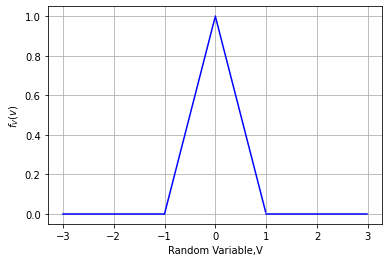
\includegraphics[width=\columnwidth] {solutions/2018/june/50/Assignment_3_Fig_1.png}
    \caption{The PDF of V}
    \label{june2018-50fig:The PDF of V}
\end{figure}

The CDF of V is defined as,
\begin{equation}
    F_V(v) = \Pr\brak{V \le v}
\end{equation}
Now for $ v \le 0 $,
 \begin{align}
    \Pr\brak{V\le v} &=  \int_{-\infty}^{v}f_{V}(v) \,dv  \\
          &=  \int_{-1}^{v} (1+v) \,dv  \\
          &=  \left(\dfrac{v^2}{2}+v \right) \Biggr|_{-1}^{v}  \\
          &=   \left(\left(\dfrac{v^2}{2}+v \right) - \left(\dfrac{1}{2} -1 \right)\right) \\
          &= \dfrac{v^2+2v +1}{2}
\end{align}
Similarly for $v \le 1$,
\begin{align}
    \Pr\brak{V\le v} &=  \int_{-\infty}^{v}f_{V}(v) \,dv  \\
          &=  \dfrac{1}{2} + \int_{0}^{v}(1-v)\,dz  \\
          &=  \dfrac{-v^2+2v+1}{2}
\end{align}

The CDF is as below: 
\begin{align}
\label{june2018-50eq:cdf_v}
F_{V}(v)  = 
\begin{cases}
0 & v < -1
\\
\dfrac{v^2+2v + 1}{2} &  v \le 0
\\
\dfrac{-v^2+2v+1}{2} &  v \le 1
\\
1 & v > 1
\end{cases}
\end{align}

The plot for CDF of $V $ can be observed at figure \ref{june2018-50fig:The CDF of V}\\

\begin{figure}[!ht]
       \centering
    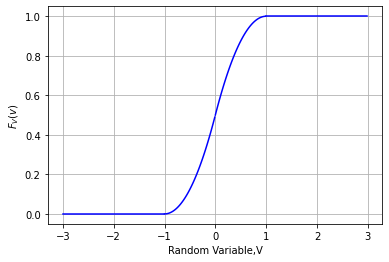
\includegraphics[width=\columnwidth] {solutions/2018/june/50/Assignment_3_Fig_2.png}
    \caption{The CDF of V}
    \label{june2018-50fig:The CDF of V}
\end{figure}

We need  $\pr{Z-W >\frac{1}{2}}$ where $Z = max(X,Y)$ and $W = min(X,Y)$. Now,

\begin{align}
\label{june2018-50eq:pdf_v}
Z-W  = 
\begin{cases}
X-Y & \text{for } X \geq Y
\\
Y-X & \text{for } X < Y
\end{cases}
\end{align}

Therefore,
\begin{align}
    \pr{Z-W >\frac{1}{2}} &= \pr{X-Y>\frac{1}{2},X \geq Y} \nonumber \\
    &+\pr{Y-X > \frac{1}{2}, X < Y}\\
    &= \pr{X-Y>\frac{1}{2}} +\pr{Y-X>\frac{1}{2}}\\
    &= \pr{V > \frac{1}{2}} + \pr{-V > \frac{1}{2}}\\
    &= 1 - \pr{V \leq \frac{1}{2}} + \pr{V < \frac{-1}{2}}\\
    &= 1-F_V(\frac{1}{2}) + F_V(-\frac{1}{2})\\
    &= 1 -\frac{7}{8} + \frac{1}{8}\\
    &= \frac{1}{4}
\end{align}

Hence the correct answer is option (C).




% \item Consider a Markov Chain with state space $S = \cbrak{1,2, 3}$ and transition matrix
% \begin{align}
% P = 
% \begin{blockarray}{c@{\hspace{1pt}}rrr@{\hspace{3pt}}}
%             & 1   & 2 & 3 \\
%         \begin{block}{r@{\hspace{3pt}}@{\hspace{1pt}}
%     (@{\hspace{1pt}}rrr@{\hspace{1pt}}@{\hspace{1pt}})}
%         1 &  0 & \frac{1}{2} & \frac{1}{2}   \\ [2mm]
%         2 & \frac{1}{2}  & 0 & \frac{1}{2}\\ [2mm]
%         3 & \frac{1}{2}  &  \frac{1}{2} & 0  \\ [2mm]
% %
%         \end{block}
%     \end{blockarray}
% \end{align}
% %
% Let $\vec{\pi}$ be a stationary distribution of the Markov chain and $d(1)$ denote the
% period of state 1.  Which of the following statements are correct?
% \begin{enumerate}
% \item $d(1) = 1$
% \item $d(1) = 2$
% \item $\pi_1 = \frac{1}{2}$
% \item $\pi_1 = \frac{1}{3}$
% \end{enumerate}
% \solution
% %
\begin{figure}
\begin{center}
\usetikzlibrary{automata, positioning}
    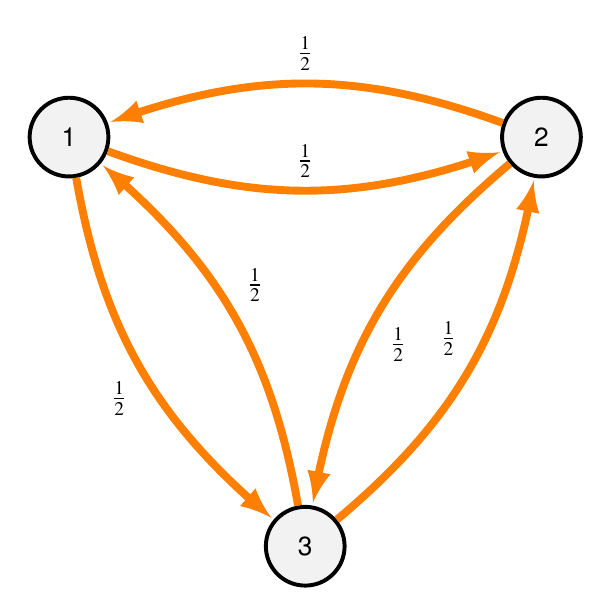
\begin{tikzpicture}[font=\sffamily]
        % Setup the style for the states
        \tikzset{node style/.style={state, 
                                    minimum width=1cm,
                                    line width=0.5mm,
                                    fill=gray!10!white}}

        % Draw the states
        \node[node style] at (0, 0)     (1)     {1};
        \node[node style] at (6, 0)     (2)     {2};
        \node[node style] at (3, -5.196) (3) 	{3};

        % Connect the states with arrows
        \draw[every loop,
              auto=right,
              line width=1mm,
              >=latex,
              draw=orange,
              fill=orange]
            (1)     edge[bend right=20]            node {$\frac{1}{2}$} (3)
            (1)     edge[bend right=20, auto=left] node {$\frac{1}{2}$} (2)
            (2)     edge[bend right=20]            node {$\frac{1}{2}$} (1)
            (2)     edge[bend right=20, auto=left] node {$\frac{1}{2}$} (3)
            (3) edge[bend right=20]            node {$\frac{1}{2}$} (1)
            (3) edge[bend right=20, auto=left] node {$\frac{1}{2}$} (2);
    \end{tikzpicture}  
    \caption{State transition diagram}
\end{center}
    \end{figure}    
    \begin{enumerate}
    \item{ The period of state 1 i.e, $d(1)$ is given as:
    \begin{align}
    d(1)=GCD\{n : P_{11}^n > 0\} \label{eq:solutions/2018/june/105/eq1a}
    \end{align}
     For $n=1$,
    \begin{align}
    \vec{P}=\myvec{0&\frac{1}{2}&\frac{1}{2}\\\frac{1}{2}&0&\frac{1}{2}\\\frac{1}{2}&\frac{1}{2}&0}\\
    \end{align}
    For $n=2$,
    \begin{align}
    \vec{P}^2=\myvec{\frac{1}{2}&\frac{1}{4}&\frac{1}{4}\\\frac{1}{4}&\frac{1}{2}&\frac{1}{4}\\\frac{1}{4}&\frac{1}{4}&\frac{1}{2}}\\
    \end{align}
    For $n=3$,
    \begin{align}
    \vec{P}^3=\myvec{\frac{1}{4}&\frac{3}{8}&\frac{3}{8}\\\frac{3}{8}&\frac{1}{4}&\frac{3}{8}\\\frac{3}{8}&\frac{3}{8}&\frac{1}{4}}\\
    \end{align}
        For $n=4$,
    \begin{align}
    \vec{P}^4=\myvec{\frac{3}{8}&\frac{5}{16}&\frac{5}{16}\\\frac{5}{16}&\frac{3}{8}&\frac{5}{16}\\\frac{5}{16}&\frac{5}{16}&\frac{3}{8}}
    \end{align}
Thus $P_{11}^n$ follows the sequence, that is defined as:
\begin{align}
    P_{11}^n= 
\begin{cases}
	0,& \text{if } n=1\\
    \frac{1}{2},& \text{if } n=2\\
    \frac{1}{2}(P_{11}^{n-1}+P_{11}^{n-2}),& \text{if } n >2
\end{cases}
\end{align}
    Since, for $n>1$, $P_{11}^n>0$
    \begin{align}
    d(1)=GCD\{2,3,4,5\cdots\}\\
    \therefore d(1)=1 \label{eq:solutions/2018/june/105/eq1}
    \end{align}
    Thus statement a is correct}\\
    \item{As calucalted above in \ref{eq:solutions/2018/june/105/eq1}, $d(1)=1$\\
    Thus statement b is incorrect.}\\
    \item{For stationary distribution,
    \begin{align}
    &\sum_{i=1}^{i=n} \pi_i = 1 \\
    &\implies\myvec{1&1&1}\myvec{\pi_1\\\pi_2\\\pi_3}=1\label{eq:solutions/2018/june/105/eq2}
    \end{align}
    Also for a stationary distribution,
    \begin{align}
    &\pi \vec{P} = \pi \\
    &(\pi \vec{P})^T = \pi^T \\
    &\vec{P}^T\pi^T=\pi^T\\
    &\implies (\vec{P}^T-\vec{I})\pi^T=0\\
    &\myvec{-1&\frac{1}{2}&\frac{1}{2}\\\frac{1}{2}&-1&\frac{1}{2}\\\frac{1}{2}&\frac{1}{2}&-1}\myvec{\pi_1\\\pi_2\\\pi_3}=\myvec{\pi_1\\\pi_2\\\pi_3} \label{eq:solutions/2018/june/105/eq3}  
\end{align}
    The given equation \ref{eq:solutions/2018/june/105/eq2}, \ref{eq:solutions/2018/june/105/eq3} can be written as:\\
    \begin{align}
    \myvec{-1&\frac{1}{2}&\frac{1}{2}\\\frac{1}{2}&-1&\frac{1}{2}\\\frac{1}{2}&\frac{1}{2}&-1\\1&1&1}\myvec{\pi_1\\\pi_2\\\pi_3}=\myvec{0\\0\\0\\1}
    \end{align}
    We need to solve the augmented matrix to row reduced echelon form to get the solution,    
    \begin{align}
    \myvec{-1&\frac{1}{2}&\frac{1}{2}&\vrule&0\\\frac{1}{2}&-1&\frac{1}{2}&\vrule&0\\\frac{1}{2}&\frac{1}{2}&-1&\vrule&0\\1&1&1&\vrule&1}\xleftrightarrow{R_4=R_4+R_1}\\\myvec{-1&\frac{1}{2}&\frac{1}{2}&\vrule&0\\\frac{1}{2}&-1&\frac{1}{2}&\vrule&0\\\frac{1}{2}&\frac{1}{2}&-1&\vrule&0\\0&\frac{3}{2}&\frac{3}{2}&\vrule&1}\xleftrightarrow{R_1=-R_1}\\\myvec{1&-\frac{1}{2}&-\frac{1}{2}&\vrule&0\\\frac{1}{2}&-1&\frac{1}{2}&\vrule&0\\\frac{1}{2}&\frac{1}{2}&-1&\vrule&0\\0&\frac{3}{2}&\frac{3}{2}&\vrule&1}\xleftrightarrow{R_2=R_2-\frac{R_1}{2}, R_3=R_3-\frac{R_1}{2}}\\\myvec{1&-\frac{1}{2}&-\frac{1}{2}&\vrule&0\\0&-\frac{3}{4}&\frac{3}{4}&\vrule&0\\0&\frac{3}{4}&-\frac{3}{4}&\vrule&0\\0&\frac{3}{2}&\frac{3}{2}&\vrule&1}\xleftrightarrow{R_3=R_3+R_2, R_4=R_4+2R_2}\\\myvec{1&-\frac{1}{2}&-\frac{1}{2}&\vrule&0\\0&-\frac{3}{4}&\frac{3}{4}&\vrule&0\\0&0&0&\vrule&0\\0&0&3&\vrule&1}\xleftrightarrow{R_2=-\frac{4}{3}R_2}\\\myvec{1&-\frac{1}{2}&-\frac{1}{2}&\vrule&0\\0&1&-1&\vrule&0\\0&0&0&\vrule&0\\0&0&3&\vrule&1}\xleftrightarrow{R_1=R_1+\frac{1}{2}R_2}\\\myvec{1&0&-1&\vrule&0\\0&1&-1&\vrule&0\\0&0&0&\vrule&0\\0&0&3&\vrule&1}\xleftrightarrow{R_3 \leftrightarrow R_4}\\\myvec{1&0&-1&\vrule&0\\0&1&-1&\vrule&0\\0&0&3&\vrule&1\\0&0&0&\vrule&0}\xleftrightarrow{R_3=\frac{R_3}{3}}\\\myvec{1&0&-1&\vrule&0\\0&1&-1&\vrule&0\\0&0&1&\vrule&\frac{1}{3}\\0&0&0&\vrule&0}\xleftrightarrow{R_1=R_1+R_3, R_2=R_2+R_3}\\\myvec{1&0&0&\vrule&\frac{1}{3}\\0&1&0&\vrule&\frac{1}{3}\\0&0&1&\vrule&\frac{1}{3}\\0&0&0&\vrule&0}
    \end{align}
    Hence,
    \begin{align}
    \pi_1=\pi_2=\pi_3=\frac{1}{3} \label{eq:solutions/2018/june/105/eq10}
    \end{align}
    Thus statement c is incorrect
    }\\
    \item{As, calculated in \ref{eq:solutions/2018/june/105/eq10}, $\pi_1=\frac{1}{3}$\\
    Thus statement d is correct}
    \end{enumerate}
Hence, statements a and d are correct.


\end{enumerate}

% \section{December 2017}
% \renewcommand{\theequation}{\theenumi}
\renewcommand{\thefigure}{\theenumi}
\renewcommand{\thetable}{\theenumi}
\begin{enumerate}[label=\thesection.\arabic*.,ref=\thesection.\theenumi]
\numberwithin{equation}{enumi}
\numberwithin{figure}{enumi}
\numberwithin{table}{enumi}

\item Let $\vec{A}$ be a real symmetric matrix and  $\vec{B}=\vec{I}+i\vec{A}$, where $i^2=-1$. Then choose the correct option.
\begin{enumerate}
	\item  $\vec{B}$ is invertible if and only if $\vec{A}$ is invertible.
	\item All Eigenvalues of $\vec{B}$ are necessarily real.
	\item $\vec{B}-\vec{I}$ is necessarily invertible.
	\item $\vec{B}$ is necessarily invertible.
\end{enumerate}
%
\solution
See Table \ref{eq:solutions/2017/dec/29/table:1}.

\onecolumn
\begin{longtable}{|l|l|}
\hline
\multirow{3}{*}{} & \\
Statement 1. &$\vec{B}$ is invertible if and only if $\vec{A}$ is  invertible.\\
\hline
& \\
False statement& Matrix $\vec{B}$ is invertible even if $\vec{A}$ is non invertible.\\
\hline
Example:&Consider a matrix \\&\parbox{12cm}{\begin{align}
 \vec{A}=\myvec{
1 &0 \\
0&0}\label{eq:solutions/2017/dec/29/eq1}\end{align}}\\& a real non invertible,symmetric matrix.\\&\parbox{12cm}{\begin{align}
&\implies\vec{B}=\myvec{1 & 0\\ 0 & 1}+i\myvec{1 & 0\\ 0 & 0}=\myvec{1+i & 0\\ 0 & 1  }\label{eq:solutions/2017/dec/29/eq2}\end{align}}\\ 

&is invertible even if $\vec{A}$ is non invertible.\\
\hline

%\pagebreak
%\hline
\multirow{3}{*}&\\
Statement 2. & All Eigenvalues of $\vec{B}$ are necessarily real.\\
\hline
&\\
False statement& Matrix $\vec{B}$ can have complex Eigenvalues.\\
\hline
Proof  :& Eigen values of $\vec{B}$ = Eigen values of     
($\vec{I}$) + i (Eigen values of $\vec{A}$).
\\&Clearly from \eqref{eq:solutions/2017/dec/29/eq2} above Eigen values of $\vec{B}$ are  $1$ and $1+i$   respectively.\\
& Hence $\vec{B}$ can also have complex Eigen value.\\
     \hline
\multirow{3}{*} & \\ 
Statement 3.  & $\vec{B}-\vec{I}$ is necessarily invertible.\\
\hline
&\\
False statement& $\vec{B}-\vec{I}=i\vec{A}$ will be invertible if $\vec{A}$, is invertible.\\\hline
&\\
Proof: & We have $\vec{B}-\vec{I}=i\vec{A}$\\
&$\implies \vec{B-I}=i\vec{A}=\myvec{i & 0\\ 0 & 0}$,from \eqref{eq:solutions/2017/dec/29/eq1}\\
 &Hence $\vec{B-I}$ is not invertible,unless $\vec{A}$ is invertible. \\
\hline
\multirow{3}{*}&\\
Statement 4. & $\vec{B}$ is necessarily invertible.\\
\hline
& \\
Correct Statement:& Matrix $\vec{B}$ has non zero Eigen values corresponding to Eigenvector $X$ .\\
\hline
Proof:& Let $X$ be an Eigen vector of $\vec{A}$ corresponding to Eigen value $\lambda$\\
&\\
&also,$\lambda\epsilon \mathbb{R}$\\
&\\
&$\implies$ $\vec{A}$$X$=$\lambda X $\\
&\\
&$\therefore$ $\vec{B}$$X=(\vec{I}+i\vec{A})X$= $\vec{I}$$X$+i$\vec{A}$$X$= $X$+$i\lambda$$X$\\
&\\
& $\implies$$\vec{B}$$X$ = $(1+i\lambda)$$X$\\
& Therefore, $1+i\lambda$ is an Eigen value of $\vec{B}$,\\
& corresponding to Eigen vector $X$,which are non zero.\\
& Hence, $\vec{B}$ is necessarily invertible.\\
\hline
\caption{Solution summary}
\label{eq:solutions/2017/dec/29/table:1}
\end{longtable}





\twocolumn
\item Let $\vec{A}=\myvec{0&1\\-1&1}$. Then the smallest positive integer n such that $\vec{A}^n=\vec{I}$ is
%
\\
\solution
{\em Property of eigen values of A: }
%\label{eq:solutions/2017/dec/30/section:prop}
Let $\vec{A}$ be an arbitary $n\times n$ matrix of complex numbers with eigen values $\lambda_1,\lambda_2,\hdots,\lambda_n$. Then  the eigen values of k\textsuperscript{th} power of $\vec{A}$, that is the eigen values of $\vec{A}^k$, for any positive integer k are $\lambda_1^k,\lambda_2^k,\hdots,\lambda_n^k$.
Let us calculate the eigen values of $\vec{A}$.
\begin{align}
\vec{A}=\myvec{0&1\\-1&1}\\
\det({\vec{A}-\lambda\vec{I}})=0\\
\mydet{-\lambda&1\\-1&1-\lambda}=0\\
-\lambda(1-\lambda)+1=0\\
\lambda^2-\lambda+1=0\\
\implies \lambda=\frac{-1\pm \sqrt{3}i}{2}
\end{align}
From the above property,
%\ref{eq:solutions/2017/dec/30/section:prop}, 
the eigen values of $\vec{A}^n$ are $\lambda^n$. Also as it is given that $\vec{A}^n=\vec{I}$, 
\begin{align}
\implies \lambda^n=1\\
\implies \brak{\frac{-1\pm \sqrt{3}i}{2}}^n=1
\end{align}
Clearly $n\ne 1$. For $n=2$,
\begin{align}
\brak{\frac{-1\pm \sqrt{3}i}{2}}^2=\frac{-1\mp \sqrt{3}i}{2}
\end{align}
For $n=4$,
\begin{align}
\brak{\frac{-1\pm \sqrt{3}i}{2}}^4=\frac{-1\pm \sqrt{3}i}{2}
\end{align}
For $n=6$,
\begin{align}
\brak{\frac{-1\pm \sqrt{3}i}{2}}^6=1
\end{align}
Hence $n=6$ is the smallest positive integer.

%
\item Let $\vec{A} = \myvec{1&-1&1\\1&1&1\\2&3&\alpha}$ and $\vec{b}= \myvec{1\\3\\\beta}$. Then the system $\vec{AX}=\vec{b}$ over the real numbers has\\
\begin{enumerate}
    \item No solution when $\beta \ne 7$
    \item Infinite number of solutions when $\alpha \ne 2$
    \item Infinite number of solutions when $\alpha = 2$ and $\beta \ne 7$
    \item A unique solution if $\alpha \ne 2$
\end{enumerate}
%
\solution
First we derive the Row Reduced Echelon Form (RREF) of the augmented matrix of the system $\vec{AX} = \vec{b}$ as follows,
\begin{align}
\myvec{1&-1&1&1\\1&1&1&3\\2&3&\alpha&\beta}&\xleftrightarrow[R_3=R_3-2R_1]{R_2=R_2-R_1}\myvec{1&-1&1&1\\0&2&0&2\\0&5&\alpha-2&\beta-2}\\
&\xleftrightarrow{R_2=\frac{1}{2}R_2}\myvec{1&-1&1&1\\0&1&0&1\\0&5&\alpha-2&\beta-2}\\
&\xleftrightarrow{R_1=R_1+R_2}\myvec{1&0&1&2\\0&1&0&1\\0&5&\alpha-2&\beta-2}\\
&\xleftrightarrow{R_3=R_3-5R_2}\myvec{1&0&1&2\\0&1&0&1\\0&0&\alpha-2&\beta-7}\label{eq:solutions/2017/dec/31/eq}
\end{align}
From the RREF of the augmented matrix of the system $\vec{AX} = \vec{b}$ in \eqref{eq:solutions/2017/dec/31/eq} we make the following observations for different values of $\alpha$ and $\beta$ in Table \ref{eq:solutions/2017/dec/31/table}.
, 
\begin{table}[ht!]
\begin{center}
\begin{tabular}{|c|c|}
\hline
Values & Observations\\
\hline
& Then the existence of solution and \\
$\beta \ne 7$ & the number of solutions will entirely \\
& depend on  value of $\alpha$\\
\hline
& Then RREF in \eqref{eq:solutions/2017/dec/31/eq} will contain \\
$\alpha = 2$ & Zero Row in $R_3$. Moreover solvability\\
$\beta \ne 7$ & condition will not satisfy. \\
& $\implies$ system will have Zero solutions\\
\hline
& RREF in \eqref{eq:solutions/2017/dec/31/eq} will have all pivots\\
$\alpha \ne$ 2 & $\implies$ RREF in \eqref{eq:solutions/2017/dec/31/eq} will be fullrank\\
& $\implies$ $\vec{AX}=\vec{b}$ have unique solution.\\
\hline
\end{tabular}
\end{center}
\caption{}
\label{eq:solutions/2017/dec/31/table}
\end{table}\\
Hence, if $\alpha \ne 2$ then the system $\vec{AX} = \vec{b}$ has unique solution.

%
\item Consider a Markov chain $\{X_n \: | \: n \geq 0\}$ with state space $\{1,2,3\}$ and transition matrix
\begin{align}
    \vec{P} = \myvec{0 & \frac{1}{2} & \frac{1}{2} \\
    \frac{1}{2} & 0 & \frac{1}{2} \\
    \frac{1}{2} & \frac{1}{2} & 0} \nonumber
\end{align}
Then, $P(X_3 = 1 \: | \: X_0 = 1)$ equals
%
\\
\solution
%
%
The three step transitional probabilities are given as,
\begin{align}
    P(X_3 = j \: | \: X_0 = i) = P(X_{n+3} = j \: | \: X_n = i) = \nonumber \\
    (\vec{P}^3)_{ij} \: for \: any \: n
\end{align}

\begin{align} \label{eq:solutions/2017/dec/51/eq:3_1}
    \vec{P}^3 = \myvec{0 & \frac{1}{2} & \frac{1}{2} \\
    \frac{1}{2} & 0 & \frac{1}{2} \\
    \frac{1}{2} & \frac{1}{2} & 0}^3 = 
    \myvec{\frac{1}{4} & \frac{3}{8} & \frac{3}{8} \\
    \frac{3}{8} & \frac{1}{4} & \frac{3}{8} \\
    \frac{3}{8} & \frac{3}{8} & \frac{1}{4}}
\end{align}
From \eqref{eq:solutions/2017/dec/51/eq:3_1},
\begin{align}
    P(X_3 = 1 \: | \: X_0 = 1) = (\vec{P}^3)_{11} = \frac{1}{4}
\end{align}

%
%\item 
%
%\\
%\solution
%See Table \ref{eq:solutions/2017/dec/75/table:1}.

\onecolumn
\begin{longtable}{|l|l|}
\hline
\multirow{3}{*}{} & \\
Statement 1. & A  is necessarily diagonalizable over $\vec{R}$\\
\hline
& \\
False statement& Matrix A is diagonalizable if and only if there is a basis of $\vec{R}^3 $consisting of\\
& eigenvectors of A.\\
Example:&Consider a matrix\\&\parbox{12cm}{\begin{align}
 \myvec{
1 &1 &0\\
0&1&1\\
0&0&4}\end{align}}\\
&Eigen values are:\\
&\parbox{12cm}{\begin{align}
 \myvec{
1 -\lambda &1 &0\\
0&1-\lambda&1\\
0&0&4-\lambda}=0.
\implies\lambda_1=1,\lambda_2=4\end{align}}\\
&\parbox{12cm}{\begin{align}
  \lambda_1=1\text { has eigen vector}
 \myvec{1\\0\\0} \text{and} 
  \lambda_2=4 \text{ has eigen vector}
\myvec{1\\3\\9}
\end{align}}\\
 & We have found only two linearly independent eigenvectors for A,not diagonalisable
\\
\hline
\multirow{3}{*}&\\
Statement 2. & If A has distinct real  eigen values
 than  it is diagonalizable over$\vec{R}$\\
\hline
&\\
True statement& Distinct real eigenvalues implies linearly independent eigenvectors .\\
& and if a matrix has n linearly independent vectors than it is  diagonalizable.\\
\hline
Proof  1:& \textbf{Distinct eigen values implies linearly independent vectors that spans entire space.}\\&Consider 2 eigen vectors $\vec{v}$,$\vec{w}$  with eigen values $\lambda$,$\mu$ respectively.\\
& such that $\lambda\neq\mu$\\
 &\parbox{12cm}{\begin{align}
    \alpha(\vec{v})+\beta(\vec{w})=0\label{eq:solutions/2017/dec/75/eq2}\\
     \alpha A(\vec{v})+\beta A(\vec{w})=0\\
     \alpha \lambda\vec{v}+\beta\mu\vec{w}=0\label{eq:solutions/2017/dec/75/eq3}
     \end{align}}\\
     & Multiplying $\eqref{eq:solutions/2017/dec/75/eq2}$with -$\lambda$ and subtracting from $\eqref{eq:solutions/2017/dec/75/eq3}$ we have,\\
   & \parbox{12cm}{\begin{align}  
  \beta(\mu-\lambda)\vec{w}=0 \label{eq:solutions/2017/dec/75/eq1}
  \end{align}}\\
  & eigen values are distinct $(\mu-\lambda)\neq 0$ .
  From equation$\eqref{eq:solutions/2017/dec/75/eq1}$ we have, $\beta=0$\\
  & substituting $\beta=0$ in  equation $\eqref{eq:solutions/2017/dec/75/eq2}$we have,$\alpha=0$.As, $\vec{v}\neq 0$\\
  & \textbf{which proves that vectors are linearly independent}.\\
  
  Proof 2:
 & \textbf{If a matrix has n linearly independent vectors than it is diagonalizable}\\
 & If\myvec{
\vec{p_1} &\vec{p_2}&\cdots&\vec{p_n} 
}are n independent eigen vectors then,
 $A\vec{p_1}=\lambda \vec{p_1},\cdots ,A\vec{p_n}=\lambda \vec{p_n}$\\
&\parbox{12cm}{\begin{align}{D}=\myvec{\lambda_1&0&\cdots&0\\
0&\lambda_2&\cdots&0\\
\vdots&\vdots&\vdots&\vdots\\
0&0&\cdots&\lambda_n}
 \and{P}=\myvec{
\vec{P_1}& \vec{P_2}&\cdots& \vec{P_n}
}\end{align}}\\
& Now, $A\vec{P_i}=\lambda_i\vec{P_i}$ $\implies$ ${A}{P}={P}{D}$\\
& so,${P^{-1}}{AP}={D}$ is a diagonal matrix.\\
    \hline
\multirow{3}{*} & \\ 
Statement 3.  & If A has distinct real  eigen values
 than  it is diagonalizable over$\vec{C}$\\
\hline
&\\
True statement& If A is an $N \times N$ complex matrix with n distinct eigenvalues, then any set of\\
& n corresponding eigenvectors form a basis for $\vec{C}^n$\\ .
&\\
Proof: &It is sufficient to prove that the set of eigenvectors is linearly independent \\
&which is proved in statement 2.\\
 Example:&\parbox{12cm}{\begin{align}A=\myvec{
4& 0 &-2\\
2& 5 &4\\
0& 0 &5
}\end{align}}\\
& Eigen values of A are:\\
& \parbox{12cm}{\begin{align}\lambda_1=2,\lambda_2=3 , \lambda_3=6\end{align}}\\
\hline
& Eigen vectors are:\\&\parbox{12cm}{\begin{align}x_1=\myvec{
-1\\1\\0
},
x_ 2=\myvec{
1\\1\\1
},
x_3=\myvec{
-1\\ - 1\\ 2
}\end{align}}
\\
 & Matrix A is diagonalizable because there is a basis of $\vec{C}^3 $consisting of\\
& eigenvectors of A.\\
\hline
\multirow{3}{*}&\\
Statement 4. & If all eigen values are non zero than it is diagonalizable over $\vec{C}$\\
\hline
& \\
False Statement:& Matrix would be diagonalizable if and only if it has linearly independent eigenvectors .\\
\hline
Example:&Consider a matrix\\&\parbox{12cm}{\begin{align}
 \myvec{
1 &1 &0\\
0&1&1\\
0&0&4}\end{align}}\\
&Eigen values are:\\
&\parbox{12cm}{\begin{align}
 \myvec{
1 -\lambda &1 &0\\
0&1-\lambda&1\\
0&0&4-\lambda}=0.
\implies\lambda_1=1,\lambda_2=4\neq 0\end{align}}\\
&\parbox{12cm}{\begin{align}
  \lambda_1=1\text { has eigen vector}
 \myvec{1\\0\\0} \text{and} 
  \lambda_2=4 \text{ has eigen vector}
\myvec{1\\3\\9}
\end{align}}\\
 & We have found only two linearly independent eigenvectors for A,not diagonalisable.\\
 &\\
\hline
\caption{Solution summary}
\label{eq:solutions/2017/dec/75/table:1}
\end{longtable}

   


\item 	Let $\vec{A}$ be an $m\times n$ matrix with rank $r$. If the linear system $\vec{A}\vec{X} = \vec{b}$ has a solution for each $\vec{b} \in \mathbf{R}^{m}$, then
	\begin{enumerate}
		\item $m=r$
		\item the column space of $\vec{A}$ is a proper subspace of $\mathbf{R}^{m}$ 
		\item the null space of $\vec{A}$ is a non-trivial subspace of $\mathbf{R}^{n}$ whenever $m=n$
		\item $m\geq n$ implies $m=n$
	\end{enumerate}
%
\solution
	{\em Theorem}
	
	\begin{theorem}\label{eq:solutions/2017/dec/72/thm1}
		Consider the $m\times n$ system Ax = b, with either b $\neq$ 0 or b = 0. We distinguish the following cases:
		\begin{enumerate}
			\item $\textbf{Unique Solution}$: If rank[A,b] = rank(A) = n $\leq$ m, then and only then the system has a unique solution. In this case, indeed as many as $m-n$ equations are redundant. And the solution $\vec{X} = {\vec{A}^{-1}\vec{b}}$. This is called as $\textbf{Exactly Determined}$.
			\item $\textbf{No Solution}$: If rank[A,b] $>$ rank(A) which necessarily implies $\Vec{b} \neq 0$ and m $>$ rank(A), then and only then the system has no solution. This is called as $\textbf{Overdetermined}$.
		\end{enumerate}
	\end{theorem}
See Table \ref{eq:solutions/2017/dec/72/table}
%	
		If the columns of an $m\times n$ matrix $\Vec{A}$ span $\vec{R}^{m}$ then the equation $\vec{A}\vec{x}=\vec{b}$ is consistent for each $\Vec{b}$ in $\vec{R}^{m}$. \\ \\
	The $\textbf{null space}$ of $\vec{A}$ is defined to be 
	
	\begin{align}\label{eq:solutions/2017/dec/72/eq1}
		Null(\vec{A}) = \{ \vec{x} \in \mathbf{R}^{n} \, \vert \, \vec{A}\vec{x} = 0 \}
	\end{align}
%	
	%	Let $\vec{A}$ be given as
	
	\begin{align} \label{eq:solutions/2017/dec/72/eq2}
		\vec{A} = \myvec{-3&-2&4 \\ 14&8&-18 \\ 4&2&-4}
	\end{align}
	
	Reduced Row Echelon form is
	
	\begin{align}
		RREF\left(\vec{A}\right) = \myvec{1&0&0 \\ 0&1&0 \\ 0&0&1}
	\end{align}
	$\therefore$ the only possible nullspace of the matrix $\vec{A}$ is $\myvec{0\\0\\0}$.\\
	
	
	Let $\vec{B}$ be given as
	
	\begin{align} \label{eq:solutions/2017/dec/72/eq3}
		\vec{B} = \myvec{-3&-2&4 \\ 14&8&-18 \\ 4&2&-4 \\ 28&16&-36 \\ 8&4&-8}
	\end{align}
	
	Reduced Row Echelon form is
	
	\begin{align}
		RREF\left(\vec{B}\right) = \myvec{1&0&0 \\ 0&1&0 \\ 0&0&1 \\ 0&0&0 \\ 0&0&0}
	\end{align}
	$\therefore$ the rank of matrix $\vec{B} = 3$.
	
	\begin{table*}[!ht]
%\centering
		\begin{tabular}{|l|l|}
			\hline
			Options & Observations\\
			\hline
			& \\
			& The rank of any matrix $\vec{A}$ is the dimension of its column space. When  \\
			$m = r$&  the number of rows ($m$) is equal to the rank ($r$) of the matrix, then \\
			&  their linear combination gives us span of $\vec{R}^{m}$.\\
			& \\
			& $\therefore$ This statement is $\textbf{True}$. \\
			& \\
			\hline 
			& \\
			& Any subspace of a vector space $\vec{V}$ other than $\vec{V}$ itself is considered a \\
			the column & proper subspace of $\vec{V}$. Which means that linear combination of $\vec{A}$\\
			space of $\vec{A}$ & will span less than $m$. That will make the resultant\\
			is a proper & $\vec{b}$ span strictly less than $m$.\\ 
			subspace of & But it is given that $\vec{b} \in \mathbf{R}^{m}$, which is contradicting.\\  
			$\mathbf{R}^{m}$ & \\
			& $\therefore$ This statement is $\textbf{False}$. \\
			& \\
			\hline
			& \\
			the null & From $\eqref{eq:solutions/2017/dec/72/eq2}$ we see that even when $m = n$ then also we are getting a\\ 
			space of $\vec{A}$ & trivial nullspace. \\
			is a non-trivial& \\
			subsapce of $\mathbf{R}^{n}$& \\
			whenever $m=n$& $\therefore$ This statement is $\textbf{False}$. \\
			& \\
			\hline
			& \\
			& It is given that the number of rows are greater than the column, and it \\
			$m \geq n$ & is given that there exists a solution. If we refer to theorem $\eqref{eq:solutions/2017/dec/72/thm1}$ we \\
			implies & see that the corresponding system will be $\textbf{Exactly Determined}$ system. \\
			$m=n$ & \\
			& As an example, it will look like $\eqref{eq:solutions/2017/dec/72/eq3}$.\\
			& \\
			& $\therefore$ This statement is $\textbf{True}$. \\
			& \\
			\hline
		\end{tabular}
\caption{Solution}
\label{eq:solutions/2017/dec/72/table}
	\end{table*}
	

\item Let $\vec{M}$ =$\cbrak{\myvec{a&b\\c&d} : a,b,c,d \in \mathbb{Z} \text{ and eigen values of} \vec{A} \in \mathbb{Q}}$ \label{main}
\begin{enumerate}
    \item $\vec{M}$ is empty
    \item $\vec{M}$ =\cbrak{\myvec{a&b\\c&d} : a,b,c,d \in \mathbb{Z}}
    \item If $\vec{A}$ $\in$ $\vec{M}$ then the eigen values of $\vec{A}$ $\in$ $\mathbb{Z}$
    \item If $\vec{A}$,$\vec{B}$ $\in$ $\vec{M}$ such that $\vec{A} \vec{B}$=$\vec{I}$ then $\mydet{\vec{A}}$ $\in$ \{+1,-1\}
\end{enumerate}
%
\solution
See Table \ref{table:2017/dec/74/}.
\onecolumn
	\begin{longtable}{|l|l|}
	\hline
	\multirow{3}{*}{$\vec{M}$ is empty} & \\
	& Consider $\vec{A}$=$\vec{I}$=\myvec{1&0\\0&1}.The elements of $\vec{A}$ $\in$ $\mathbb{Z}$ and it's eigen values 1 $\in$ $\mathbb{Q}$.\\
	&So, $\vec{M}$ is not empty. \\
	& \\
	\hline
	\multirow{3}{*}{$\vec{M}$ =\cbrak{\myvec{a&b\\c&d} : a,b,c,d \in \mathbb{Z}}} & \\
	& Let $\vec{A}$=\myvec{0&-1\\1&0} where elements of $\vec{A}$ $\in$ $\mathbb{Z}$.The characteristic equation can be \\ 
	& written as :\\
	& \\
	& \qquad \qquad \qquad$ \lambda^2+1 = 0 \implies \lambda = \pm i$ \\
	& \\
	& We see that $\lambda$ $\in$ $\mathbb{C}$ which is contradicting the main definition of $\vec{M}$ .So,this \\
	& is not correct. \\
	& \\
	\hline
	\multirow{3}{*}{Eigen values of $\vec{A}$ $\in$ $\mathbb{Z}$} & \\
	& Given ,$\vec{A}$ $\in$ $\vec{M}$.Let $\lambda_1$,$\lambda_2$ be the eigen values of $\vec{A}$.The characteristic polynomial \\ 
	&can be written as:\\
	& \\
	& \qquad \qquad \qquad$ \lambda^2-tr\brak{\vec{A}}\lambda +\det{\vec{A}}= 0 $ where $tr\brak{\vec{A}}=\lambda_1+\lambda_2,\det{\vec{A}}=\lambda_1\lambda_2$\\
	& \\
	& Given the eigen values $\lambda\_1$,$\lambda\_2$  $\in$ $\mathbb{Q}$,For this to be possible the discriminant \\
	& of above equation should $\in$ $\mathbb{Z}$\\
	& \qquad \qquad \qquad$\sqrt{(\lambda_1+\lambda_2)^2-4\lambda_1\lambda_2} \in \mathbb{Z}$ \\
	& \qquad \qquad$\implies \sqrt{(\lambda_1-\lambda_2)^2} \in \mathbb{Z}$ \\
	& \qquad \qquad$\implies \lambda_1-\lambda_2 \in \mathbb{Z}$ 
	This is possible when both $\lambda_1$,$\lambda_2$ $\in$ $\mathbb{Z}$.\\
	& \\
	\hline
	\multirow{3}{*}{If $\vec{A} \vec{B}$=$\vec{I}$ then $\mydet{\vec{A}}$ $\in$ \{+1,-1\}} 
	& \\
	& As $\vec{A}$,$\vec{B}$ $\in$ $\vec{M}$,$\implies$ $\mydet{\vec{A}}$,$\mydet{\vec{B}}$ $\in$ $\mathbb{Z}$ \\
	& Given $\vec{A}\vec{B}$=$\vec{I}$ $\implies$ $\mydet{\vec{A}}\mydet{\vec{B}}$=1\\
	& This is possible only when $\mydet{\vec{A}}$=$\mydet{\vec{B}}$= $\pm$ 1\\
	& \\
	\hline
	\multirow{3}{*}{Conclusion} & \\
	& options 3) and 4) are correct.\\
    & \\
	\hline
\caption{Solution}
\label{table:2017/dec/74/}
    \end{longtable}

%
\item Let A be a $3\times 3$  matrix  with real entries.Identify  the correct statements.
\begin{enumerate}

\item A  is necessarily diagonalizable over $\vec{R}$

\item If A has distinct real  eigen values than  it is diagonalizable over$\vec{R}$

\item If A has distinct eigen values than  it is diagonalizable over $\vec{C}$

\item If all eigen values are non zero than it is diagonalizable over $\vec{C}$
\end{enumerate}
%
\solution
See Table \ref{eq:solutions/2017/dec/75/table:1}.

\onecolumn
\begin{longtable}{|l|l|}
\hline
\multirow{3}{*}{} & \\
Statement 1. & A  is necessarily diagonalizable over $\vec{R}$\\
\hline
& \\
False statement& Matrix A is diagonalizable if and only if there is a basis of $\vec{R}^3 $consisting of\\
& eigenvectors of A.\\
Example:&Consider a matrix\\&\parbox{12cm}{\begin{align}
 \myvec{
1 &1 &0\\
0&1&1\\
0&0&4}\end{align}}\\
&Eigen values are:\\
&\parbox{12cm}{\begin{align}
 \myvec{
1 -\lambda &1 &0\\
0&1-\lambda&1\\
0&0&4-\lambda}=0.
\implies\lambda_1=1,\lambda_2=4\end{align}}\\
&\parbox{12cm}{\begin{align}
  \lambda_1=1\text { has eigen vector}
 \myvec{1\\0\\0} \text{and} 
  \lambda_2=4 \text{ has eigen vector}
\myvec{1\\3\\9}
\end{align}}\\
 & We have found only two linearly independent eigenvectors for A,not diagonalisable
\\
\hline
\multirow{3}{*}&\\
Statement 2. & If A has distinct real  eigen values
 than  it is diagonalizable over$\vec{R}$\\
\hline
&\\
True statement& Distinct real eigenvalues implies linearly independent eigenvectors .\\
& and if a matrix has n linearly independent vectors than it is  diagonalizable.\\
\hline
Proof  1:& \textbf{Distinct eigen values implies linearly independent vectors that spans entire space.}\\&Consider 2 eigen vectors $\vec{v}$,$\vec{w}$  with eigen values $\lambda$,$\mu$ respectively.\\
& such that $\lambda\neq\mu$\\
 &\parbox{12cm}{\begin{align}
    \alpha(\vec{v})+\beta(\vec{w})=0\label{eq:solutions/2017/dec/75/eq2}\\
     \alpha A(\vec{v})+\beta A(\vec{w})=0\\
     \alpha \lambda\vec{v}+\beta\mu\vec{w}=0\label{eq:solutions/2017/dec/75/eq3}
     \end{align}}\\
     & Multiplying $\eqref{eq:solutions/2017/dec/75/eq2}$with -$\lambda$ and subtracting from $\eqref{eq:solutions/2017/dec/75/eq3}$ we have,\\
   & \parbox{12cm}{\begin{align}  
  \beta(\mu-\lambda)\vec{w}=0 \label{eq:solutions/2017/dec/75/eq1}
  \end{align}}\\
  & eigen values are distinct $(\mu-\lambda)\neq 0$ .
  From equation$\eqref{eq:solutions/2017/dec/75/eq1}$ we have, $\beta=0$\\
  & substituting $\beta=0$ in  equation $\eqref{eq:solutions/2017/dec/75/eq2}$we have,$\alpha=0$.As, $\vec{v}\neq 0$\\
  & \textbf{which proves that vectors are linearly independent}.\\
  
  Proof 2:
 & \textbf{If a matrix has n linearly independent vectors than it is diagonalizable}\\
 & If\myvec{
\vec{p_1} &\vec{p_2}&\cdots&\vec{p_n} 
}are n independent eigen vectors then,
 $A\vec{p_1}=\lambda \vec{p_1},\cdots ,A\vec{p_n}=\lambda \vec{p_n}$\\
&\parbox{12cm}{\begin{align}{D}=\myvec{\lambda_1&0&\cdots&0\\
0&\lambda_2&\cdots&0\\
\vdots&\vdots&\vdots&\vdots\\
0&0&\cdots&\lambda_n}
 \and{P}=\myvec{
\vec{P_1}& \vec{P_2}&\cdots& \vec{P_n}
}\end{align}}\\
& Now, $A\vec{P_i}=\lambda_i\vec{P_i}$ $\implies$ ${A}{P}={P}{D}$\\
& so,${P^{-1}}{AP}={D}$ is a diagonal matrix.\\
    \hline
\multirow{3}{*} & \\ 
Statement 3.  & If A has distinct real  eigen values
 than  it is diagonalizable over$\vec{C}$\\
\hline
&\\
True statement& If A is an $N \times N$ complex matrix with n distinct eigenvalues, then any set of\\
& n corresponding eigenvectors form a basis for $\vec{C}^n$\\ .
&\\
Proof: &It is sufficient to prove that the set of eigenvectors is linearly independent \\
&which is proved in statement 2.\\
 Example:&\parbox{12cm}{\begin{align}A=\myvec{
4& 0 &-2\\
2& 5 &4\\
0& 0 &5
}\end{align}}\\
& Eigen values of A are:\\
& \parbox{12cm}{\begin{align}\lambda_1=2,\lambda_2=3 , \lambda_3=6\end{align}}\\
\hline
& Eigen vectors are:\\&\parbox{12cm}{\begin{align}x_1=\myvec{
-1\\1\\0
},
x_ 2=\myvec{
1\\1\\1
},
x_3=\myvec{
-1\\ - 1\\ 2
}\end{align}}
\\
 & Matrix A is diagonalizable because there is a basis of $\vec{C}^3 $consisting of\\
& eigenvectors of A.\\
\hline
\multirow{3}{*}&\\
Statement 4. & If all eigen values are non zero than it is diagonalizable over $\vec{C}$\\
\hline
& \\
False Statement:& Matrix would be diagonalizable if and only if it has linearly independent eigenvectors .\\
\hline
Example:&Consider a matrix\\&\parbox{12cm}{\begin{align}
 \myvec{
1 &1 &0\\
0&1&1\\
0&0&4}\end{align}}\\
&Eigen values are:\\
&\parbox{12cm}{\begin{align}
 \myvec{
1 -\lambda &1 &0\\
0&1-\lambda&1\\
0&0&4-\lambda}=0.
\implies\lambda_1=1,\lambda_2=4\neq 0\end{align}}\\
&\parbox{12cm}{\begin{align}
  \lambda_1=1\text { has eigen vector}
 \myvec{1\\0\\0} \text{and} 
  \lambda_2=4 \text{ has eigen vector}
\myvec{1\\3\\9}
\end{align}}\\
 & We have found only two linearly independent eigenvectors for A,not diagonalisable.\\
 &\\
\hline
\caption{Solution summary}
\label{eq:solutions/2017/dec/75/table:1}
\end{longtable}

   


\twocolumn
\item Let $V$ be a vector space over $C$ of all the polynomials in a variable $X$ of degree atmost 3. Let $D:V \xrightarrow{} V$ be the linear operator given by differentiation with respect to $X$. Let $A$ be the matrix of $D$ with respect to some 
basis for $V$. Which of the following are true? \\
\begin{enumerate}
\item A is nilpotent matrix \\
\item A is diagonalizable matrix \\ 
\item the rank of A is 2 \\
\item the Jordan canonical form of A is
\begin{align}\nonumber
    \myvec{0&1&0&0\\
       0&0&1&0\\
       0&0&0&1\\
       0&0&0&0}
\end{align}
\end{enumerate}
%
\solution
See Tables \ref{eq:solutions/2017/dec/76/table0}, \ref{eq:solutions/2017/dec/76/table2} and \ref{eq:solutions/2017/dec/76/table1}


\begin{table*}[ht!]
\begin{center}
\begin{tabular}{|c|c|}
\hline
& \\
Given & $V$ be a vector space over $C$ of all the polynomials in a variable $X$ of degree atmost 3\\
& $D$ : $P_3 \xrightarrow{} P_3$ \\ 
& \\
& $D:V\xrightarrow{}V$ be the linear operator given by differentiation wrt $X$\\
& $D(P(x)) \xrightarrow{}$ $P'(x)$ \\
& \\
& $A$ be the matrix of $D$ wrt some basis for $V$ \\
& Assume basis for $V$ be $\{1,x,x^2,x^3\}$ \\
& \\
\hline
\end{tabular}
\end{center}
\caption{}
\label{eq:solutions/2017/dec/76/table0}
\end{table*}
\begin{table*}[ht!]
\begin{center}
\begin{tabular}{|c|c|}
\hline
&\\
Matrix & $D(1)$ = $0$ = $0.1+0.x+$\\
& $0.x^2+0.x^3$\\
& $D(1)$ = $\myvec{0\\0\\0\\0}$ \\
& $D(x)$ = $1$ = $1.1+0.x+$\\
& $0.x^2+0.x^3$\\
& $D(x)$ = $\myvec{1\\0\\0\\0}$ \\
& $D(x^2)$ = $2x$ = $0.1+2.x+$\\
& $0.x^2+0.x^3$\\
& $D(x^2)$ = $\myvec{0\\2\\0\\0}$ \\
& $D(x^3)$ = $3x^2$ = $0.1+0.x+$\\
& $3.x^2+0.x^3$\\
& $D(x^3)$ = $\myvec{0\\0\\3\\0}$ \\
& Matrix $A$ = $\myvec{0&1&0&0\\
                0&0&2&0\\
                0&0&0&3\\
                0&0&0&0}$\\
&\\
\hline
& \\
Inference & An $n\times n$ matrix with $\lambda$\\
& as diagonal elements, ones on the\\
& super diagonal and zeroes in all\\
& other entries is nilpotent with\\
& minimal polynomial $(A-\lambda I)^n$\\
&\\
\hline
& \\
Nilpotent & $A$ = $\myvec{0&1&0&0\\
                0&0&2&0\\
                0&0&0&3\\
                0&0&0&0}$\\
& \\
& All eigen values of matrix $A$\\
& is $0$\\
& Thus, above matrix is \\
& nilpotent matrix \\
& Thus, above statement \\
& is true\\
& \\
\hline
\end{tabular}
\end{center}
\caption{}
\label{eq:solutions/2017/dec/76/table2}
\end{table*}
\begin{table*}[ht!]
\begin{center}
\begin{tabular}{|c|c|}
\hline
Diagonalizable & $A$ = $\myvec{0&1&0&0\\
                0&0&2&0\\
                0&0&0&3\\
                0&0&0&0}$\\
& $Rank(A)$ + $nullity(A)$ = no of column\\
& $Rank(A)$ = 3, no of column = 4 \\
& $nullity(A)$ = 4 - 3 = 1\\
& means there exists only one\\
& linearly independent eigen vector\\
& corresponding to $0$ eigen values\\
& Thus,matrix $A$ is not Diagonalizable.\\
& Thus, above statement is false\\
& \\
\hline
& \\
Rank & $A$ = $\myvec{0&1&0&0\\
                0&0&2&0\\
                0&0&0&3\\
                0&0&0&0}$\\
& \\
& Rank of matrix $A$ is $3$\\
& Thus, above statement is false\\
& \\
\hline
& \\
Jordan CF & Assume characteristic polynomial of \\
& matrix $A$ is $c_A(x)$ \\
& $c_A(x)$ = $x^4$ \\
& Assume minimal polynomial of\\
& $A$ is $m_A(x)$\\
& $m_A(x)$ always divide $c_A(x)$ \\
& $m_A(x)$ = $\{x,x^2,x^3,x^4\}$\\
& Minimal polynomial always annihilates\\
& its matrix.Thus,we see that\\
& $m_A(A)$ = $\{A=0,A^2=0,A^3=0,A^4=0\}$\\
& But we see that neither A is zero matrix\\
& nor $A^2$ and $A^3$ equal to zero\\
& but $A^4$ is equal to zero.Thus,$x^4$\\
& is minimal polynomial.\\
& Algebraic Multiplicity = $a_M$($\lambda$ = 0) = 4\\
& Geometric Multiplicity = $g_M$($\lambda$ = 0) = \\
& $nullity(A-0I)$ = $nullity(A)$ = 1\\
& Hence, Jordan form of block size 4\\
& Using Inference, $\vec{J} = \myvec{\lambda & 1 & 0 & 0 \\ 
                        0 & \lambda & 1 & 0\\ 
                        0 & 0 & \lambda & 1\\
                        0 & 0 & 0 & \lambda }$ \\
& $\lambda$ = 0 \\ 
& $\myvec{0&1&0&0\\
       0&0&1&0\\
       0&0&0&1\\
       0&0&0&0}$\\
& which is same as given in\\
& the question. Thus,statement is true \\
& \\
\hline
\end{tabular}
\end{center}
\caption{}
\label{eq:solutions/2017/dec/76/table1}
\end{table*}

\item For every $4 \times 4$ real symmetric non-singular matrix $\vec{A}$ there 
exists a positive integer $p$ such that

    \begin{enumerate}
        \item $p\vec{I}+\vec{A}$ is positive definite
        \item $\vec{A}^p$ is positive definite
        \item $\vec{A}^{-p}$ is positive definite
        \item $\text{exp}(p\vec{A})-\vec{I}$ is positive definite
        \end{enumerate}
\solution
%
A matrix is real symmetric implies its eigen values are real and eigen vectors are orthogonal,that is its eigen value decomposition is
\begin{align}
 \vec{A}=\vec{P}\vec{D}\vec{P}^T
\end{align}
$\vec{D}$ is the diagonal matrix containing the real eigen values of $\vec{A}$\\
$\vec{P}$ has the corresponding eigen vectors
\begin{align}
    \vec{P}\vec{P}^T=\vec{P}^T\vec{P}=\vec{I}
\end{align}
A real matrix is positive definite if 
\begin{align}
    \vec{x}^T\vec{A}\vec{x}>0\\
    \implies  \vec{x}^T\lambda\vec{x}>0\\
    \implies \lambda \vec{x}^T\vec{x}>0\\
    \implies \lambda>0
\end{align}
In other words, all the eigen values of $A$ are positive
See Table \ref{eq:solutions/2017/dec/77/table:0}

Let $\vec{A}$ be
\begin{align}
    \vec{A}=\vec{P}\vec{D}\vec{P}^T\\
    \vec{D}=\myvec{\lambda_1&0&0&0\\0&\lambda_2&0&0\\0&0&\lambda_3&0\\0&0&0&\lambda_4}
\end{align}



\begin{table*}[!t]
    \centering
    \begin{tabular}{|l|l|}
    \hline

    \textbf{OPTIONS} & \textbf{DERIVATIONS}\\
    \hline
     Choice 1 & 
      \parbox{12cm}{\begin{align}
         p\vec{I}+\vec{A}=\vec{P}(p\vec{I})\vec{P}^T+\vec{P}\vec{D}\vec{P}^T\\
   = \vec{P}\vec{D}_1\vec{P}^T\\
    \vec{D}_1=\myvec{\lambda_1+p&0&0&0\\0&\lambda_2+p&0&0\\0&0&\lambda_3+p&0\\0&0&0&\lambda_4+p}
    \end{align}}\\
     & Some of the eigen values of $\vec{A}$ may be negative.\\
     & All the eigen values in $\vec{D}_1$ are positive only if \\
     & \parbox{12cm}{\begin{align}
          p>|\lambda_i|\text{  } \forall i \in [1,4]
     \end{align}}\\
      
      \hline
      Choice 2 & 
       \parbox{12cm}{\begin{align}
          \vec{A}^2=\vec{A}\vec{A}\\
    =(\vec{P}\vec{D}\vec{P}^T)(\vec{P}\vec{D}\vec{P}^T)\\
    =\vec{P}\vec{D}^2\vec{P}^T\\
    \text{Similarly, }\vec{A}^p=\vec{P}\vec{D}^p\vec{P}^T\\
    \vec{D}^p=\myvec{\lambda_1^p&0&0&0\\0&\lambda_2^p&0&0\\0&0&\lambda_3^p&0\\0&0&0&\lambda_4^p}
       \end{align}}\\
       & $\vec{A}^{p}$ is positive definite only if $p$ is even.\\
       \hline
      Choice 3& 
        \parbox{12cm}{\begin{align}
           \vec{A}^{-p}=\vec{P}\vec{D}^{-p}\vec{P}^T\\
    \vec{D}^{-p}=\myvec{\lambda_1^{-p}&0&0&0\\0&\lambda_2^{-p}&0&0\\0&0&\lambda_3^{-p}&0\\0&0&0&\lambda_4^{-p}}
       \end{align}}\\
       & $\vec{A}^{-p}$ is positive definite only if $p$ is even.\\
       \hline
      Choice 4 &
        \parbox{12cm}{\begin{align}
          \text{exp}(p\vec{A})=\sum_{k=0}^\infty \frac{(p\vec{A})^k}{k!}\\
     \implies  \text{exp}(p\vec{A})-\vec{I}=\vec{P} \text{exp}(p\vec{D})\vec{P}^T-\vec{P}\vec{I}\vec{P}^T\\
     =\vec{P}( \text{exp}(p\vec{D})-\vec{I}) \vec{P}^T\\
     \text{exp}(p\vec{D})-\vec{I}=\myvec{e^{\lambda_1}-1&0&0&0\\0&e^{\lambda_2}-1&0&0\\0&0&e^{\lambda_3}-1&0\\0&0&0&e^{\lambda_4}-1}
       \end{align}}\\
       & $\vec{A}$ is non-singular\\
        & \parbox{12cm}{\begin{align}
   \implies \forall i \in [1,4], \lambda_i\neq0\\
   e^{\lambda_i}<1
\end{align}}\\
 & So, exp$(p\vec{A})-\vec{I}$ is not positive definite.\\
       \hline
    \end{tabular}
    \caption{Solution}
\label{eq:solutions/2017/dec/77/table:0}
\end{table*}
 From the table,the choices would be option 1,2,3





\item Let $\vec{A}$ be an $m \times n$ matrix of rank $m$ with $n>m$. If for some non-zero real number $\alpha$, we have $\vec{x^TAA^Tx} = \alpha\vec{x^Tx}$, for all $x \in \vec{R^m}$, then $\vec{A^TA}$ has,
\begin{enumerate}

\item  exactly two distinct eigenvalues.

\item  0 as an eigenvalue with multiplicity $n-m$.

\item  $\alpha$ as a non-zero eigenvalue.

\item  exactly two non-zero distinct eigenvalues.
\end{enumerate}
%
\solution
Refer Table \ref{eq:solutions/2017/dec/78/table:1}.


\begin{table*}[ht!]
\begin{center}
\resizebox{\columnwidth}{!}
{
\begin{tabular}{|l|l|}
\hline
\textbf{Given} & \textbf{Derivation} \\[0.5ex]
\hline
\text{Given} & 
\text{$\vec{A}$ is a $m \times n$ matrix of rank $m$ with $n>m$}. \\
& A non-zero real number $\alpha$.\\
& To find eigenvalues of $\vec{A^TA}$.
\\ [0.5ex]
\hline
\text{Eigenvalues of $\vec{AA^T}$} & 
\text{$\vec{AA^T}$ is a $m \times m$ matrix and $\vec{A^TA}$ is a $n \times n$ matrix.}\\
& Let, $\lambda$ be a non-zero eigen value of $\vec{A^TA}$.\\
& \parbox{10cm}{\begin{align}
    \vec{A^TAv} = \lambda \vec{v} \quad \vec{v} \in \vec{R^n}\\
    \vec{AA^TAv} = \lambda \vec{Av}\\
    \text{Let,} \quad \vec{x} = \vec{Av} \quad \vec{x} \in \vec{R^m}\\
    \vec{AA^Tx} = \lambda \vec{x}\\
    \vec{x^TAA^Tx} = \lambda \vec{x^Tx}\\
    \text{Given}, \quad \vec{x^TAA^Tx} = \alpha\vec{x^Tx}\\
    \implies \alpha\vec{x^Tx} = \lambda \vec{x^Tx} \label{eq:solutions/2017/dec/78/eq:eq18}
\end{align}} \\
& From equation \eqref{eq:solutions/2017/dec/78/eq:eq18}, $\lambda = \alpha$ as $\norm{\vec{x}} \not = 0$\\
& As rank($\vec{A^TA}$) = rank($\vec{A}$) = $m$ and equation \eqref{eq:solutions/2017/dec/78/eq:eq18} satisfies the condition in question.\\
&Therefore the only non-zero eigen value is $\alpha$\\
& $\vec{A^TA}$ has an eigenvalue $\alpha$ with multiplicity $m$.
\\ [0.5ex]
\hline
\text{Eigenvalues of $\vec{A^TA}$} & 
$\vec{A^TA}$ is a $n \times n$ matrix. Given $n > m$, \\\\
&We know that, $\vec{A^TA}$ and $\vec{AA^T}$ have same number of non-zero eigenvalues\\& and if one of them has more number of eigenvalues than the other \\&then these eigenvalues are zero.\\
& 1. From above, as $\alpha$ is non-zero, $\vec{A^TA}$ has $\alpha$ as its eigenvalue with multiplicity $m$ \\
& 2. $\vec{A^TA}$ has $0$ as its eigenvalue with multiplicity $n-m$\\
& 3. Therefore, the two distinct eigenvalues of $\vec{A^TA}$ are $\alpha$ and $0$.
\\ [0.5ex]
\hline
\end{tabular}
}
\end{center}

\caption{Explanation}
\label{eq:solutions/2017/dec/78/table:1}
\end{table*}

Refer Table \ref{eq:solutions/2017/dec/78/table:2}.

\begin{table*}[ht]
\begin{center}
\resizebox{\columnwidth}{!}
{
\begin{tabular}{|c|c|}
\hline
& \\
$\vec{A^TA}$ has exactly two distinct eigenvalues.
& True statement\\
\hline
& \\
$\vec{A^TA}$ has 0 as an eigenvalue with multiplicity $n-m$
& True statement\\
\hline
& \\
$\vec{A^TA}$ has $\alpha$ as a non-zero eigenvalue
&  True statement\\
\hline
& \\
$\vec{A^TA}$ has exactly two non-zero distinct eigenvalues.
& False statement\\
\hline
\end{tabular}
}
\end{center}
\caption{Solution}
\label{eq:solutions/2017/dec/78/table:2}
\end{table*}

\item %
Consider a Markov chain with five states $\{1,2,3,4,5\}$ and transition matrix
\begin{align}
    P=\myvec{\frac{1}{2} & 0 & 0 & \frac{1}{2} & 0\\
            0 & \frac{1}{7} & 0 & 0&\frac{6}{7}\\
              \frac{1}{5} & \frac{1}{5} & \frac{1}{5} & \frac{1}{5} & \frac{1}{5}\\ \frac{1}{3} & 0 & 0 & \frac{2}{3} & 0 \\
              0 & \frac{5}{8} & 0 & 0 & \frac{3}{8}}
\end{align}
Which of the following are true?
\begin{enumerate}
\item 3 and 1 are in the same communicating class
\item 1 and 4 are in the same communicating class
\item 4 and 2 are in the same communicating class
\item 2 and 5 are in the same communicating class
\end{enumerate}
%
\solution
See Tables \ref{eq:solutions/2017/dec/105/table0} and \ref{eq:solutions/2017/dec/105/table1}

\begin{table*}[!ht]
\centering
\resizebox{2\columnwidth}{!}
{
\begin{tabular}{|l|l|}
	\hline
	\multirow{3}{*}{Accessibility of states} 
	& \\
	& We say that state $j$ is accessible from state $i$, written as $i \rightarrow j$, if $p^{(n)}_{ij}>0$\\ in Markov's chain
	& for some n. Every state is accessible from itself since $p^{(0)}_{ii}=1$\\
	&\\
	\hline
	\multirow{3}{*}{Communication between} & \\
	& Two states $i$ and $j$ are said to communicate, written as $i\leftrightarrow j$, if they\\ states
	& are accessible from each other. In other words,\\
	&\\
  	& \qquad \qquad  \qquad $i \leftrightarrow j  \;  \textrm{ means } \;  i \rightarrow j  \textrm{ and }  j \rightarrow i.$ \\
    	& \\
    	\hline
    	\multirow{3}{*}{Communicating class} & \\
	& For each Markov chain, there exists a unique decomposition of the \\
	& state space $S$ into a sequence of disjoint subsets $C_1, C_2, . . .,$\\
	&\\
    	&  \qquad \qquad  \qquad$S=\bigcup_{i=1}^{\infty}C_i$\\
    	&\\
    	& in which each subset has the property that all states within it communicate.\\
    	& Each such subset is called a communication class of the Markov chain.\\
    	&\\
    \hline
\end{tabular}
}
\caption{Definition and Result used}
\label{eq:solutions/2017/dec/105/table0}
\end{table*}
%\usepackage{longtable}
%\begin{table*}
%\centering
\onecolumn
	\begin{longtable}{|l|l|}
		\hline
		\multirow{3}{*}{Drawing Transition diagram} 
		& \\
		& 
		
		
\tikzset{every picture/.style={line width=0.75pt}} %set default line width to 0.75pt        
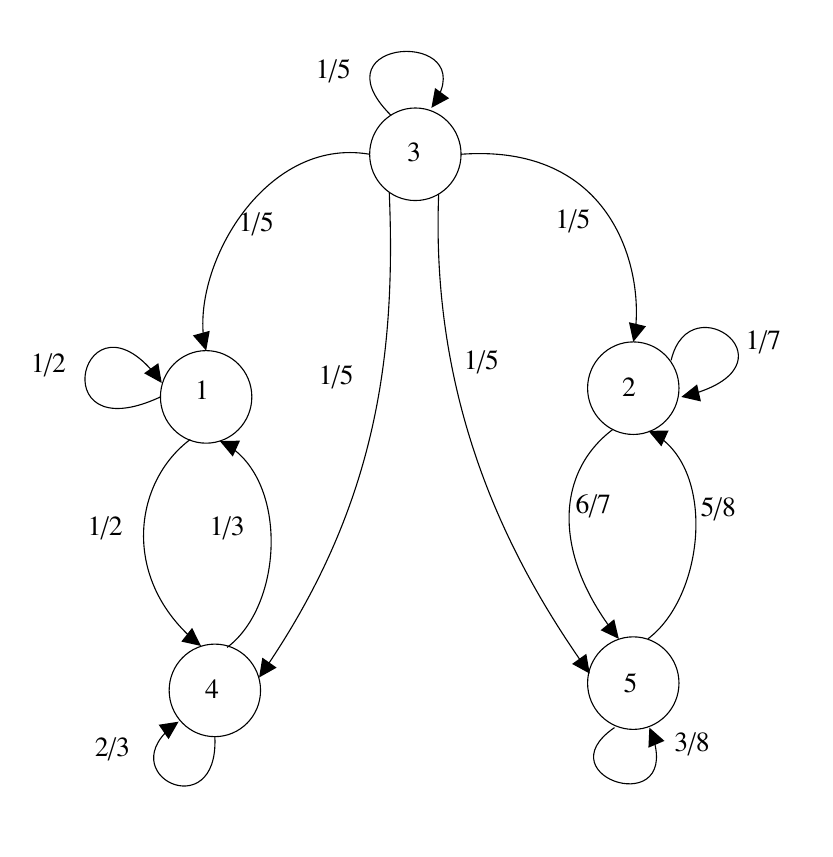
\begin{tikzpicture}[x=0.75pt,y=0.75pt,yscale=-0.7,xscale=0.7]
%uncomment if require: \path (0,714); %set diagram left start at 0, and has height of 714
%Shape: Ellipse [id:dp29836895541013164] 
\draw   (286,156.85) .. controls (286,139.26) and (300.08,125) .. (317.45,125) .. controls (334.82,125) and (348.9,139.26) .. (348.9,156.85) .. controls (348.9,174.44) and (334.82,188.7) .. (317.45,188.7) .. controls (300.08,188.7) and (286,174.44) .. (286,156.85) -- cycle ;
%Shape: Ellipse [id:dp4858180433459096] 
\draw   (142,323.85) .. controls (142,306.26) and (156.08,292) .. (173.45,292) .. controls (190.82,292) and (204.9,306.26) .. (204.9,323.85) .. controls (204.9,341.44) and (190.82,355.7) .. (173.45,355.7) .. controls (156.08,355.7) and (142,341.44) .. (142,323.85) -- cycle ;
%Shape: Ellipse [id:dp10893001214881792] 
\draw   (436,317.85) .. controls (436,300.26) and (450.08,286) .. (467.45,286) .. controls (484.82,286) and (498.9,300.26) .. (498.9,317.85) .. controls (498.9,335.44) and (484.82,349.7) .. (467.45,349.7) .. controls (450.08,349.7) and (436,335.44) .. (436,317.85) -- cycle ;
%Shape: Ellipse [id:dp31584444241771226] 
\draw   (148,525.85) .. controls (148,508.26) and (162.08,494) .. (179.45,494) .. controls (196.82,494) and (210.9,508.26) .. (210.9,525.85) .. controls (210.9,543.44) and (196.82,557.7) .. (179.45,557.7) .. controls (162.08,557.7) and (148,543.44) .. (148,525.85) -- cycle ;
%Shape: Ellipse [id:dp6845584977543557] 
\draw   (436,520.85) .. controls (436,503.26) and (450.08,489) .. (467.45,489) .. controls (484.82,489) and (498.9,503.26) .. (498.9,520.85) .. controls (498.9,538.44) and (484.82,552.7) .. (467.45,552.7) .. controls (450.08,552.7) and (436,538.44) .. (436,520.85) -- cycle ;
%Curve Lines [id:da40673715992947246] 
\draw    (212.24,513.63) .. controls (288.82,402.26) and (304.45,300.14) .. (299.5,183.32) ;
\draw [shift={(209.9,517)}, rotate = 304.9] [fill={rgb, 255:red, 0; green, 0; blue, 0 }  ][line width=0.08]  [draw opacity=0] (12.5,-6.01) -- (0,0) -- (12.5,6.01) -- cycle    ;
%Curve Lines [id:da5133467038577342] 
\draw    (172.69,288.89) .. controls (161.52,237.16) and (212.5,144.11) .. (286,156.85) ;
\draw [shift={(173.45,292)}, rotate = 254.65] [fill={rgb, 255:red, 0; green, 0; blue, 0 }  ][line width=0.08]  [draw opacity=0] (12.5,-6.01) -- (0,0) -- (12.5,6.01) -- cycle    ;
%Curve Lines [id:da008345831811055193] 
\draw    (167.44,493.28) .. controls (114.6,449.49) and (123.1,382.7) .. (162.5,353.15) ;
\draw [shift={(169.9,495.27)}, rotate = 218.21] [fill={rgb, 255:red, 0; green, 0; blue, 0 }  ][line width=0.08]  [draw opacity=0] (12.5,-6.01) -- (0,0) -- (12.5,6.01) -- cycle    ;
%Curve Lines [id:da5634268603548509] 
\draw    (435.25,511.14) .. controls (385.72,441.07) and (327.59,334.04) .. (333.5,184.32) ;
\draw [shift={(437.5,514.32)}, rotate = 234.46] [fill={rgb, 255:red, 0; green, 0; blue, 0 }  ][line width=0.08]  [draw opacity=0] (12.5,-6.01) -- (0,0) -- (12.5,6.01) -- cycle    ;
%Curve Lines [id:da4259073730032066] 
\draw    (187.9,496.27) .. controls (227.3,466.72) and (230.27,378.53) .. (185,355.28) ;
\draw [shift={(182.9,354.27)}, rotate = 384.44] [fill={rgb, 255:red, 0; green, 0; blue, 0 }  ][line width=0.08]  [draw opacity=0] (12.5,-6.01) -- (0,0) -- (12.5,6.01) -- cycle    ;
%Curve Lines [id:da6577514807411684] 
\draw    (468.08,283.01) .. controls (475.64,242.78) and (457.71,148.87) .. (348.9,156.85) ;
\draw [shift={(467.45,286)}, rotate = 283.29] [fill={rgb, 255:red, 0; green, 0; blue, 0 }  ][line width=0.08]  [draw opacity=0] (12.5,-6.01) -- (0,0) -- (12.5,6.01) -- cycle    ;
%Curve Lines [id:da329541870026538] 
\draw    (142,323.85) .. controls (58.35,362.99) and (88.88,241.85) .. (141.3,312.08) ;
\draw [shift={(142.9,314.27)}, rotate = 234.51] [fill={rgb, 255:red, 0; green, 0; blue, 0 }  ][line width=0.08]  [draw opacity=0] (12.5,-6.01) -- (0,0) -- (12.5,6.01) -- cycle    ;
%Curve Lines [id:da3393212160499588] 
\draw    (493.5,298.66) .. controls (506.37,243.94) and (584.91,303.18) .. (503.03,323.29) ;
\draw [shift={(500.5,323.88)}, rotate = 347.23] [fill={rgb, 255:red, 0; green, 0; blue, 0 }  ][line width=0.08]  [draw opacity=0] (12.5,-6.01) -- (0,0) -- (12.5,6.01) -- cycle    ;
%Curve Lines [id:da7968400462935867] 
\draw    (477.5,490.39) .. controls (516.9,460.84) and (525.1,371.56) .. (480,348.28) ;
\draw [shift={(477.9,347.27)}, rotate = 384.44] [fill={rgb, 255:red, 0; green, 0; blue, 0 }  ][line width=0.08]  [draw opacity=0] (12.5,-6.01) -- (0,0) -- (12.5,6.01) -- cycle    ;
%Curve Lines [id:da49532662514959913] 
\draw    (455.47,487.82) .. controls (411.57,431.68) and (414.1,375.7) .. (453.5,346.15) ;
\draw [shift={(457.5,490.39)}, rotate = 231.1] [fill={rgb, 255:red, 0; green, 0; blue, 0 }  ][line width=0.08]  [draw opacity=0] (12.5,-6.01) -- (0,0) -- (12.5,6.01) -- cycle    ;
%Curve Lines [id:da618838807270425] 
\draw    (179.45,557.7) .. controls (182.46,620.43) and (105.86,583.53) .. (152.3,548.96) ;
\draw [shift={(154.5,547.39)}, rotate = 505.54] [fill={rgb, 255:red, 0; green, 0; blue, 0 }  ][line width=0.08]  [draw opacity=0] (12.5,-6.01) -- (0,0) -- (12.5,6.01) -- cycle    ;
%Curve Lines [id:da7726575310463464] 
\draw    (479.68,554.36) .. controls (503.45,616.53) and (404.27,585.93) .. (454.51,551.46) ;
\draw [shift={(478.51,551.46)}, rotate = 67.01] [fill={rgb, 255:red, 0; green, 0; blue, 0 }  ][line width=0.08]  [draw opacity=0] (12.5,-6.01) -- (0,0) -- (12.5,6.01) -- cycle    ;
%Curve Lines [id:da7210031613710599] 
\draw    (330.71,121.65) .. controls (363.66,70.1) and (246.61,75.98) .. (300.51,129.88) ;
\draw [shift={(328.51,124.88)}, rotate = 306.03] [fill={rgb, 255:red, 0; green, 0; blue, 0 }  ][line width=0.08]  [draw opacity=0] (12.5,-6.01) -- (0,0) -- (12.5,6.01) -- cycle    ;
% Text Node
\draw (164,311.21) node [anchor=north west][inner sep=0.75pt]   [align=left] {{\normalsize 1}};
% Text Node
\draw (458,309.21) node [anchor=north west][inner sep=0.75pt]   [align=left] {{\normalsize 2}};
% Text Node
\draw (171,517.21) node [anchor=north west][inner sep=0.75pt]   [align=left] {{\normalsize 4}};
% Text Node
\draw (459,512.21) node [anchor=north west][inner sep=0.75pt]   [align=left] {{\normalsize 5}};
% Text Node
\draw (310,147.21) node [anchor=north west][inner sep=0.75pt]   [align=left] {{\normalsize 3}};
% Text Node
\draw (51,292.21) node [anchor=north west][inner sep=0.75pt]   [align=left] {{\normalsize 1/2}};
% Text Node
\draw (90,404.21) node [anchor=north west][inner sep=0.75pt]   [align=left] {{\normalsize 1/2}};
% Text Node
\draw (543,276.21) node [anchor=north west][inner sep=0.75pt]   [align=left] {{\normalsize 1/7}};
% Text Node
\draw (174,404.21) node [anchor=north west][inner sep=0.75pt]   [align=left] {{\normalsize 1/3}};
% Text Node
\draw (194,195.21) node [anchor=north west][inner sep=0.75pt]   [align=left] {{\normalsize 1/5}};
% Text Node
\draw (426,389.21) node [anchor=north west][inner sep=0.75pt]   [align=left] {{\normalsize 6/7}};
% Text Node
\draw (512,391.21) node [anchor=north west][inner sep=0.75pt]   [align=left] {{\normalsize 5/8}};
% Text Node
\draw (95,556.21) node [anchor=north west][inner sep=0.75pt]   [align=left] {{\normalsize 2/3}};
% Text Node
\draw (494,553.21) node [anchor=north west][inner sep=0.75pt]   [align=left] {{\normalsize 3/8}};
% Text Node
\draw (247,90.21) node [anchor=north west][inner sep=0.75pt]   [align=left] {{\normalsize 1/5}};
% Text Node
\draw (249,300.21) node [anchor=north west][inner sep=0.75pt]   [align=left] {{\normalsize 1/5}};
% Text Node
\draw (349,290.21) node [anchor=north west][inner sep=0.75pt]   [align=left] {{\normalsize 1/5}};
% Text Node
\draw (412,193.21) node [anchor=north west][inner sep=0.75pt]   [align=left] {{\normalsize 1/5}};
\end{tikzpicture}

		
		
		\\  
		&\\
		&\\
		\hline
		\multirow{3}{*}{Checking whether the  } & \\
		& Here,\\states 3 and 1 are in the
		& State 1 is accessible from the state 3.\\same communicating class
	    	& But, State 3 is not accessible from the state 1\\
	    	& \qquad \qquad \qquad i.e.  $3 \rightarrow 1$,  $1 \nrightarrow 3$\\
	    	& \qquad \qquad \qquad$\implies \boxed{3 \nleftrightarrow 1}$\\
	    	&\\ 
	    	&Therefore, 3 and 1 are not in the same communicating class.\\
	   	&\\
	   	\hline
	   \multirow{3}{*}{Checking whether the  } & \\
		& Here,\\states 1 and 4 are in the
		& State 1 is accessible from the state 4.\\same communicating class
	    	& Also, State 4 is accessible from the state 1\\
	    	& \qquad \qquad \qquad i.e.  $3 \rightarrow 1$,  $1 \rightarrow 3$\\
	   	& \qquad \qquad \qquad$\implies \boxed{3 \leftrightarrow 1}$\\
	    	&\\ 
	    	&Therefore, 1 and 4 are in the same communicating class.\\	   	
	   	&\\	   	
	   	\hline
	   	\multirow{3}{*}{Checking whether the  } & \\
		& Here,\\states 4 and 2 are in the
		& State 2 is not accessible from the state 4.\\same communicating class
	    	& Also, State 4 is not accessible from the state 2\\
	    	& \qquad \qquad \qquad i.e.  $4 \nrightarrow 2$,  $2 \nrightarrow 4$\\
	    	\hline
	    	&\\	    	
	   	& \qquad \qquad \qquad$\implies \boxed{4 \nleftrightarrow 2}$\\
	    	&Therefore, 4 and 2 are not in the same communicating class.\\
	   	&\\
	   	\hline
	   	\multirow{3}{*}{Checking whether the  } & \\
		& Here,\\states 2 and 5 are in the
		& State 2 is accessible from the state 5.\\same communicating class
	    	& Also, State 5 is accessible from the state 2\\
	    	& \qquad \qquad \qquad i.e.  $5 \rightarrow 2$,  $2 \rightarrow 5$\\
	   	& \qquad \qquad \qquad$\implies \boxed{2 \leftrightarrow 5}$\\
	    	&\\
	    	&Therefore, 2 and 5 are in the same communicating class.\\
	   	&\\
	   	\hline
	   	\multirow{3}{*}{Conclusion} & \\
	   	&Communication classes are:\\
	   	&\\
	   	& \qquad \qquad \qquad$\boxed{S=\{1,4\}\cup \{3\} \cup \{2,5\}}$\\
	   	&\\
		&Option 2) and 4) are true.\\
	   	&\\
	   	\hline
\caption{Solution}
\label{eq:solutions/2017/dec/105/table1}
    \end{longtable}
%\end{table*}
\twocolumn


%
\item Let $X$ and $Y$ be independent exponential random variables. If $E[X]=1$ and $E[Y]=\frac{1}{2}$ then $\pr{X>2Y|X>Y}$ is
\begin{multicols}{2}
    \begin{enumerate}[label=\arabic*.]
        \item \Large$\frac{1}{2}$ \\
        \item $\frac{1}{3}$
        \item $\frac{2}{3}$ \\
        \item $\frac{3}{4}$
    \end{enumerate}
\end{multicols}
%
\solution
Since $X$ and $Y$ are exponential random variables with means'
\begin{align}
    E[X] = 1 \text{ and } E[Y] = \frac{1}{2}
\end{align}
Marginal PDFs of $X$ and $Y$  are given by
\begin{align}
    f_X(x)= e^{-x} , x>0 \\
    f_Y(y) = 2e^{-2y} , y>0
\end{align}
CDFs for $X$ and $Y$ are
\begin{align}
    F_X(b) &= \int_0^b f_X(x)\,d_x\\
           &= \int_0^b  e^{-x}\,d_x\\
           &= 1-e^{-b}
\end{align}
\begin{align}
    F_Y(b) &= \int_0^b f_Y(y)\,d_y\\
           &= \int_0^b 2e^{-2y}\,d_y\\
           &= \left[-e^{-2y}\right]_0^b\\
           &= 1-e^{-2b}
\end{align}
Now,
\begin{align}
    \pr{X>2Y|X>Y} &= \dfrac{\pr{X>2Y\,,\,X>Y} }{\pr{X>Y}}\\
                  &= \dfrac{\pr{X>2Y}}{\pr{X>Y}} \label{dec2017-59:simul1}
\end{align}
\begin{align}
    \pr{X>Y} &= \pr{Y<X}\\
             &= E[F_Y(X)]\\
             &= \int_0^\infty F_Y(X)\,f_X(x)\,d_x\\
             &= \int_0^\infty (1-e^{-2x})\,e^{-x}d_x\\
             &= \left[\frac{e^{-x}}{-1} - \frac{e^{-3x}}{-3}\right]_0^\infty\\
            &=(0+1)+\frac{1}{3}(0-1) \\
             &= \frac{2}{3} \label{dec2017-59:simul2}
\end{align}
\begin{align}
    \pr{X>2Y} &= \pr{Y<\frac{X}{2}}\\
              &= E[F_Y(X/2)]\\
              &=  \int_0^\infty F_Y(X/2)\,f_X(x)\,d_x\\
              &= \int_{0}^{\infty}(1-e^{-x})\,e^{-x}d_x\\
              &= \left[\frac{e^{-x}}{-1} - \frac{e^{-2x}}{-2}\right]_0^\infty\\
              &= (0+1) + \frac{1}{2}(0-1)\\
              &= \frac{1}{2} \label{dec2017-59:simul3}
\end{align}
Putting \eqref{dec2017-59:simul2} and \eqref{dec2017-59:simul3} in \eqref{dec2017-59:simul1}
\begin{align}
    \pr{X>2Y\,|\,X>Y} &= \frac{1/2}{2/3}\\
                  &= \frac{3}{4}
\end{align}
$\therefore$ Option 4 is the correct answer.


%\item Consider a Markov Chain with state space $\cbrak{0,1,2}$ and transition matrix
%\begin{align}
%P = 
%\begin{blockarray}{c@{\hspace{1pt}}rrr@{\hspace{3pt}}}
%         & 0   & 1   & 2 \\
%        \begin{block}{r@{\hspace{3pt}}@{\hspace{1pt}}
%    (@{\hspace{1pt}}rrr@{\hspace{1pt}}@{\hspace{1pt}})}
%        0 & \frac{1}{2} & \frac{1}{2} & 0  \\
%        1 & 0 &\frac{1}{2}  & \frac{3}{4}  \\
%%
%        2 &  \frac{1}{3} & \frac{1}{3} & \frac{1}{3}  \\
%        \end{block}
%    \end{blockarray}
%\end{align}
%For any two states $i$ and $j$, let $p_{ij}^{(n)}$ denote the $n$-step transition probability of going from $i$ to $j$.  Identify correct statements.
%\begin{enumerate}
%\item $\lim_{n \to \infty} p_{11}^{(n)} = \frac{2}{9}$
%\item $\lim_{n \to \infty} p_{21}^{(n)} = 0$
%\item $\lim_{n \to \infty} p_{32}^{(n)} = \frac{1}{3}$
%\item $\lim_{n \to \infty} p_{13}^{(n)} = \frac{1}{3}$
%\end{enumerate}

\end{enumerate}

% %\twocolumn
% \section{June 2017}
% \renewcommand{\theequation}{\theenumi}
\renewcommand{\thefigure}{\theenumi}
\begin{enumerate}[label=\thesection.\arabic*.,ref=\thesection.\theenumi]
\numberwithin{equation}{enumi}
\numberwithin{figure}{enumi}

%
\item X and Y are independent random variables each having the density
\begin{align}
    f(t) = \displaystyle\frac{1}{\pi} \frac{1}{1+{t}^2} -\infty < t < +\infty
\end{align}
Then the density function of $\displaystyle\frac{X+Y}{3}$ for \\$-\infty <$ t $< +\infty$ is\bigskip
    \begin{enumerate}\itemsep0.5cm
        \item $\displaystyle\frac{6}{\pi} \frac{1}{4+9{t}^2}$
        \item $\displaystyle\frac{6}{\pi} \frac{1}{9+4{t}^2}$
        \item $\displaystyle\frac{3}{\pi} \frac{1}{1+9{t}^2}$
        \item $\displaystyle\frac{3}{\pi} \frac{1}{9+{t}^2}$
    \end{enumerate}

%
\solution
Let us consider the random variables X and Y.
    The Characteristic function of the probability density $f(t)$ is
    \begin{align}
        g(w) =\hspace{0.2cm} & \int_{-\infty}^{\infty}  f(t) {e}^{iwt} dt                                         \\[0.2cm]
        =\hspace{0.2cm}      & \int_{-\infty}^{\infty}  \displaystyle\frac{1}{\pi} \frac{1}{1+{t}^2} {e}^{iwt} dt \\[0.2cm]
        =\hspace{0.2cm}      & e^{-\abs{w}}\hspace{0.2cm}, -\infty<w<\infty
    \end{align}
    The product of the Characteristic function of \\probability density of X and Y is
    \begin{align}
        h(w) = g_1(w) \times g_2(w) = {e}^{-2\abs{w}}
    \end{align}
    To get the probability density of X+Y, we find the inverse characteristic function of h(w). But since there is a one to one correspondence between a function and its fourier transform and
$h(w) = g(2w)$
    \begin{align}
        F_{X+Y}(t) =\hspace{0.2cm} & \frac{1}{2}f\brak{\frac{t}{2}}                                        \\[0.2cm]
        =\hspace{0.2cm}            & \frac{1}{2\pi} \frac{4}{4+{t}^2} \hspace{0.2cm},-\infty<t<\infty
    \end{align}
    We know that if a random variable M has a\\probability density $f_M(x)$, then the probability \\density of random variable kM is
    \begin{align}
        f_{kM}\brak{x} = \frac{1}{\abs{k}} f_M\brak{\frac{x}{\abs{k}}}
    \end{align}
    Probability density of $Z = \displaystyle\frac{X+Y}{3}$ given $F_{X+Y}(t)$ is
\begin{align}
    F_{Z}(t) = & 3\times \displaystyle f_{X+Y}(3t) \\
    =          & \frac{6}{\pi} \frac{1}{4+9{t}^2}
\end{align}
%
\item Let $\left\{X_{n}, n \geq 1\right\}$ be i.i.d. uniform (-1,2) random variables. Which of the following statements are true?
\begin{enumerate}[label=\alph*)]
\item $\dfrac{1}{n} \sum_{i=1}^{n} X_{i} \rightarrow 0$ almost surely
\item $\left\{\dfrac{1}{2 n} \sum_{i=1}^{n} X_{2 i}-\dfrac{1}{2 n} \sum_{i=1}^{n} X_{2 i-1}\right\}\rightarrow 0$
almost surely
\item $\sup \left\{X_{1}, X_{2}, \ldots\right\}=2$ almost surely
\item $\inf \left\{X_{1}, X_{2}, \ldots\right\}=-1$ almost surely
\end{enumerate}
\solution
We using convergence in almost surely and Strong law of large number (SLLN)
\begin{enumerate}
\item {\em Almost sure convergence : }Let $X_{1}, X_{2}, \ldots$ be an infinite sequence of random variables. We shall say that the sequence $\left\{X_{i}\right\}$ converges with probability 1 (or converges almost surely (a.s.)) to a random variable $Y$, if 
\begin{align}
\pr{\lim _{n \rightarrow \infty} X_{n}=Y}=1 \\ 
\text{and we write}, X_{n} \stackrel{a . s .}{\rightarrow} Y
\end{align} 
\item {\em SLLN : }Let $X_{n}$ be i.i.d with $\mathbf{E}\left[\left|X_{1}\right|\right]<\infty$. Then, as $n \rightarrow \infty$ , we have
\begin{align}
\dfrac{S_{n}}{n} \stackrel{\text { a.s. }}{\rightarrow} \mathbf{E}\left[X_{1}\right]\implies \dfrac{S_{n}}{n} \stackrel{\text { P }}{\rightarrow} \mathbf{E}\left[X_{1}\right]\\
,\text{where} \, S_n = X_1 + \cdots + X_n
\end{align}   
also,
\begin{align}
X_i \stackrel{a.s.}{\rightarrow} X \implies g(X_i) \stackrel{a.s.}{\rightarrow} g(X)
\label{june/2017/104Eq}  
\end{align}
\end{enumerate}
\begin{enumerate}[label=\alph*)]
\item\begin{align}
\dfrac{1}{n}\left(X_{1}+\cdots+X_{n}\right) \rightarrow E(X)\in(-1,2)\\
\text{as} \, n\rightarrow\infty,
\end{align}
according to strong law of large numbers (SLLN).\\
So, option $(\mathrm{A})$ is incorrect.
\item using this \ref{june/2017/104Eq} , we solve as
\begin{align}
\left\{\dfrac{1}{2 n} \sum_{i=1}^{n} X_{2 i}-\dfrac{1}{2 n} \sum_{i=1}^{n} X_{2 i-1}\right\}&\stackrel{a.s.}{\rightarrow}\left\{\dfrac{nX}{2 n}-\dfrac{nX}{2 n}\right\}\\
&=0
\end{align}
option $(\mathrm{B})$ is correct.
\item  Similarly, Let $M=\sup (S) .$ Then,
\begin{align}
x \leq M, &\quad \forall x \in S \\
\forall \epsilon>0,& \quad(M-\epsilon, M] \cap S \neq \emptyset
\end{align}
where, $S$ be a nonempty subset of $\mathbb{R}$ with an upper bound. Using $X_i \stackrel{a.s.}{\rightarrow} X$ this , we  conclude that
\begin{align}
\sup \left\{X_{1}, X_{2}, \ldots\right\}&=2 \;almost\; surely
\end{align}
\item Let $m=\inf (S)$. Then
\begin{align}
x \geq m, & \quad \forall x \in S \\
\forall \epsilon>0, &\quad {[m, m+\epsilon] \cap S \neq \emptyset}
\end{align}
where, $S$ be a nonempty subset of $\mathbb{R}$ with an lower bound. Again using $X_i \stackrel{a.s.}{\rightarrow} X$ this , we conclude that
\begin{align}
\inf \left\{X_{1}, X_{2}, \ldots\right\}&=-1 \;almost\; surely
\end{align}
Hence $(\mathrm{B}),(\mathrm{C})$ and $(\mathrm{D})$ are correct options.
\end{enumerate}
%
\item $X_{1}, X_{2}, \cdots$ are independent identically distributed random variables
having common density $f$. Assume $f(x)=f(-x)$ for all $x \in \mathbb{R}$. Which of the following statements is correct?
\begin{enumerate}[label=\alph*)]
\item $\dfrac{1}{n}\left(X_{1}+\cdots+X_{n}\right) \rightarrow 0$ in probability
\item $\dfrac{1}{n}\left(X_{1}+\cdots+X_{n}\right) \rightarrow 0$ almost surely
\item $\pr{\dfrac{1}{\sqrt{n}}\left(X_{1}+\cdots+X_{n}\right)<0} \rightarrow \dfrac{1}{2}$
\item $\sum_{i=1}^{n} X_{i}$ has the same distribution as $\sum_{i=1}^{n}(-1)^{i} X_{i}$
\end{enumerate}
%
\solution
We using
\begin{enumerate}[label=\alph*)]
\item 
\begin{enumerate}[label=(\arabic*)]
\item {\em Convergence in probability : }Let $X_{1}, X_{2}, \ldots$ be an infinite sequence of random variables, and let $Y$ be another random variable. Then the sequence $\left\{X_{n}\right\}$ converges in probability to $Y$, if
\begin{align}
\forall \epsilon>0, \lim _{n \rightarrow \infty} \pr{\left|X_{n}-Y\right| \geq \epsilon}=0,
\end{align}
and we write 
\begin{align}
X_{n} \stackrel{P}{\rightarrow} Y.
\end{align}
\item {\em Convergence in almost surely : }Let $X_{1}, X_{2}, \ldots$ be an infinite sequence of random variables. We shall say that the sequence $\left\{X_{i}\right\}$ converges with probability 1 (or converges almost surely (a.s.)) to a random variable $Y$, if 
\begin{align}
\pr{\lim _{n \rightarrow \infty} X_{n}=Y}=1
\end{align}
and we write
\begin{align}
X_{n} \stackrel{a . s .}{\rightarrow} Y
\end{align}
\item {\em Strong law of large number(SLLN) : }Let $X_{1}, X_{2}, \ldots$ be an infinite sequence of random variables, If $\mathbf{E}\left[\left|X_{1}\right|\right]<\infty$. Then, as $n \rightarrow \infty$ , we have 
\begin{align}
\dfrac{S_{n}}{n} \stackrel{a.s.}{\rightarrow} \mathbf{E}\left[X_{1}\right]\implies \dfrac{S_{n}}{n} \stackrel{P}{\rightarrow} \mathbf{E}\left[X_{1}\right],
\label{june/2017/50eq} \\
\text{where} ,\,S_n = X_1 + \cdots + X_n
\end{align}  
\end{enumerate}
using SLLN, $(\mathrm{B})$ are incorrect option.
\item {\em Relation between in probability and almost surely : }Let $Z, Z_{1}, Z_{2}, \ldots$ be random variables. Suppose $Z_{n} \rightarrow Z$ with probability 1. Then ,we say 
\begin{align}
 Z_n \stackrel{a.s.}{\rightarrow} Z \implies Z_n \stackrel{P}{\rightarrow} Z.
\end{align}
\eqref{june/2017/50eq}, also in probability also hold this equation. Hence $(\mathrm{A})$ is incorrect option.  
\item 
{\em Central Limit Theorem : }Let $X_{1}, X_{2}, \ldots$ be i.i.d. with finite mean $\mu$ and finite variance $\sigma^{2}$. Let $Z \sim N(0,1) .$ Set $S_{n}=X_{1}+\cdots+X_{n}$, and
\begin{align}
Z_{n}=\frac{S_{n}-n \mu}{\sqrt{n \sigma^{2}}}
\end{align}
Then as $n \rightarrow \infty$, the sequence $\left\{Z_{n}\right\}$ converges in distribution to the $Z$, i.e., $Z_{n} \stackrel{D}{\rightarrow} Z$.\\
Consider,
\begin{align}
Y=\dfrac{X_{1}+ X_{2}+ \cdots + X_n}{\sqrt{n}}
\end{align}
So,
\begin{align}
E(Y)= E\left(\dfrac{X_{1}+ X_{2}+ \cdots+X_n}{\sqrt{n}}\right)= 0\\
V(Y)= V\left(\dfrac{X_{1}+ X_{2}+ \cdots+X_n}{\sqrt{n}}\right)= \frac{1}{n}2n=2
\end{align}
\begin{align}
Y \sim N[0,2]
\end{align}
we know that,
\begin{align}
f(x)=f(-x)\implies \text{Symmetry about Zero},
\end{align}
So,
\begin{align}
\pr{Y<0}=\frac{1}{2}
\end{align}
\begin{align}
\pr{\dfrac{1}{\sqrt{n}}\left(X_{1}+\cdots+X_{n}\right)<0}=\frac{1}{2}
\end{align}
Hence$,(\mathrm{C})$ is incorrect option.
\item {\em Characteristic function : }For a scalar random variable $X$ the characteristic function is defined as the expected value of $\mathrm{e}^{i t \times}$, where $i$ is the imaginary unit, and $t \in \mathbf{R}$ is the argument of the characteristic function:
\begin{align}
\left\{\begin{array}{l}
\varphi_{X}: \mathbb{R} \rightarrow \mathbb{C} \\
\varphi_{X}(t)=\mathrm{E}\left[e^{i t X}\right]=\int_{\mathbb{R}} e^{i t x} d F_{X}(x)\\=\int_{\mathbb{R}} e^{i t x} f_{X}(x) d x=\int_{0}^{1} e^{i t Q_{X}(p)} d p
\end{array}\right.
\end{align}
Here $F_X$ is the cumulative distribution function of $X$,Consider, $\phi_{x}(t)$ is characteristic function of $X_{i}, i=1, \ldots, n.$
\begin{align}
f(x)=f(-x)\implies \phi_{x}(t)=\phi_{-x}(t)
\end{align}
Therefore,
\begin{align}
\phi_{\sum_{i=1}^{n}X_i}(t) = \phi_{X_{1}+\ldots +X_{n}}(t) &=\phi_{X_{1}}(t)\cdots\phi_{X_{n}}(t)\\
&=\left[\phi_{x}(t)\right]^{n}
\end{align}
similarly,
\begin{align}
\phi_{\sum_{i=1}^{n}(-1)^{i}X_i}(t) &= \phi_{-X_{1}}+\phi_{X_{2}}+\ldots +\phi_{(-1)^{n}X_{n}}(t)\\
&=\phi_{-X_{1}}(t) \cdot \phi_{X_{2}}(t)\cdots\phi_{(-1)^{n}X_{n}}(t)\\
&=\left[\phi_{x}(t)\right]^{n}\\
\phi_{\sum_{i=1}^{n}X_i}(t) &= \phi_{\sum_{i=1}^{n}(-1)^{i}X_i}(t)
\end{align}
$\therefore \sum_{i=1}^{n} X_{i}$ has same distribution as $\sum_{i=1}^{n}(-1)^{i} X_{i}.$\\
Hence, only $(\mathrm{D})$ is correct option.
\end{enumerate}
\item Suppose the random variable X has the following probability density funtion 
\begin{align}
    f(x)=\begin{cases}\alpha\brak{x-\mu}^{\alpha -1}e^{-\brak{x-\mu}^\alpha};&x>\mu\\
                        0                               &x\leq\mu    
    \end{cases}\nonumber
\end{align}
where $\alpha>0,-\infty <\mu<\infty$. Which of the following are correct? The hazard function of $X$ is
\begin{enumerate}
    \item an increasing function for all $\alpha>0$
    \item a decreasing function for all $\alpha >0$
    \item an increasing function for some $\alpha>0$
    \item a decreasing function for some $\alpha>0$
\end{enumerate}
%
\solution

\newcommand{\Integral}[2]{solutions/2017/june/118/figures/\ensuremath{\int\limits_{#1}^{#2}}}
For the random variable $X$, the CDF is
\begin{align}
    F(x)&=\Integral{0}{x}f(y)dy\\
        &=\Integral{0}{\mu}0 dy +\Integral{\mu}{x}\alpha\brak{y-\mu}^{\alpha -1}e^{-\brak{y-\mu}^\alpha}\\
        &=0 -e^{-\brak{y-\mu}^\alpha}\Big|_{\mu}^{x}\\
        &=1-e^{-\brak{x-\mu}^{\alpha}}
\end{align}
For X, the hazard function $H(y)$ is defined as
\begin{align}
    H(y)&=\frac{f(y)}{1-F(y)}\nonumber\\
    \implies H(y)&=\begin{cases}\frac{\alpha\brak{y-\mu}^{\alpha -1}e^{-\brak{y-\mu}^\alpha}}{1-\brak{1-e^{-\brak{y-\mu}^{\alpha}}}};&y>\mu\\
                        0                               &y\leq\mu   
    \end{cases}\nonumber\\
    &=\begin{cases}\alpha\brak{y-\mu}^{\alpha -1};&y>\mu\\
                        0                            &y\leq\mu   
    \end{cases}\nonumber
\end{align}
Differentiating $H(y)$ w.r.t. $y$
\begin{align}
    H'(y)&=\begin{cases}\alpha\brak{\alpha - 1}\brak{y-\mu}^{\alpha -2};&y>\mu\\
                        0                            &y\leq\mu   
    \end{cases}\nonumber
\end{align}
When $y\leq \mu$ then $H'(y)$ is $0$. When $y>\mu$ then $\brak{y-\mu}^{\alpha -2}$ is positive. This implies that the sign for $H'(y)$ for $y>\mu$ is decided by the sign of $\alpha\brak{\alpha -1}$.
\begin{align}
    \alpha\brak{1-\alpha}<0
    \implies 0<\alpha<1\nonumber\\
    \alpha\brak{1-\alpha}>0\implies \alpha>1 &&\text{(ignoring $\alpha<0$)}\nonumber
\end{align}
$\therefore$ The Hazard function of $X$ is decreasing when $\alpha \in \brak{0,1}$ and increasing when $\alpha \in \brak{1,\infty}$
\vspace{0.5cm}\centering \boxed{\solution{\text{Options 3, 4}}}
% \iffalse
% \begin{figure}[h!]
%     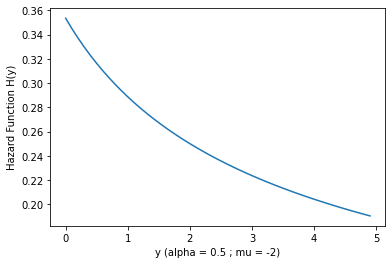
\includegraphics[width = \columnwidth]{solutions/2017/june/118/figures/Figure-1.png}
%     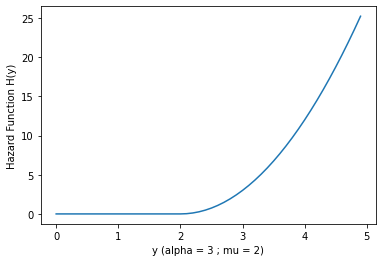
\includegraphics[width = \columnwidth]{solutions/2017/june/118/figures/Figure-2.png}
% \end{figure}
% \fi
\begin{figure}[h]
    \centering
    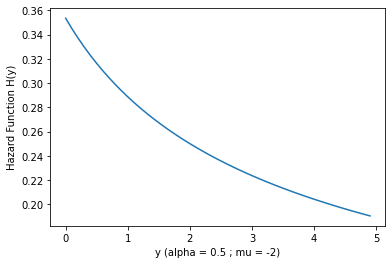
\includegraphics[width=\columnwidth-50pt]{solutions/2017/june/118/figures/Figure-1.png}
    \caption{Decreasing Hazard Function}
    \label{june/2017/118/fig:my_label1}
\end{figure}
\begin{figure}[h]
    \centering
    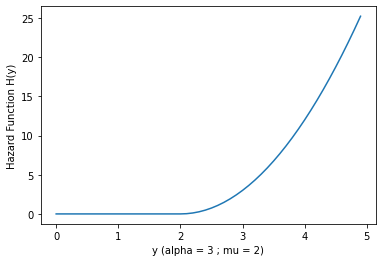
\includegraphics[width=\columnwidth-50pt]{solutions/2017/june/118/figures/Figure-2.png}
    \caption{Increasing Hazard Function}
    \label{june/2017/118/fig:my_label2}
\end{figure}


% \item $X_1$ and $X_2$ are independent Poisson variables such that $\pr{X_1=2} = \pr{X_1=1}$ and $\pr{X_2=2} = \pr{X_2=3}$. What is the variance of $(X_1 - 2X_2)$ ?
% \begin{enumerate}
%     \item 14
%     \item 4
%     \item 3
%     \item 2
% \end{enumerate}
% \solution
% For a Poisson variable X,
\begin{align}
\pr{X=k} = \frac{\lambda^{k}e^{-\lambda}}{k!}
\end{align}
Since $\pr{X_1=2} = \pr{X_1=1}$,
\begin{align}
\frac{{\lambda_1}^{2}e^{-{\lambda_1}}}{2!} &= \frac{{\lambda_1}^{1}e^{-{\lambda_1}}}{1!} \\
\lambda_1 &= 2!/1! = 2
\end{align}
Similarly, as $\pr{X_2=2} = \pr{X_2=3}$,
\begin{align}
\frac{{\lambda_2}^{2}e^{-{\lambda_2}}}{2!} &= \frac{{\lambda_2}^{3}e^{-{\lambda_2}}}{3!} \\
\lambda_2 &= 3!/2! = 3
\end{align}
Also we know for a Poisson variable X, the following holds true:
\begin{align}
\E[X] &= \lambda \\
\Var[X] &= \lambda \label{june/2017/108/eq1} \\
\Var[X] &= \E[X^2] - (\E[X])^2 \label{june/2017/108/eq2} 
\end{align}
Now, for the variance of $(X_1 - 2X_2)$
\begin{align}
\Var[X_1 - 2X_2] &= \E[(X_1 - 2X_2)^2] - (\E[X_1 - 2X_2])^2 \nonumber \\
&= \E[X_1^2 + 4X_2^2 - 4X_1X_2] \nonumber \\
&- (\E[X_1] - 2\E[X_2])^2 \nonumber \\
&= \E[X_1^2] - (\E[X_1])^2 + 4\E[X_2^2] \nonumber \\
& -4(\E[X_2])^2) + 4\E[X_1X_2] \nonumber \\
& + 4\E[X_1]\E[X_2]
\end{align}
Since the variables are independent:
\begin{align}
\E[X_1X_2] = \E[X_1]\E[X_2]
\end{align}
Substituting equations \eqref{june/2017/108/eq1} and \eqref{june/2017/108/eq2}, we get:
\begin{align}
\Var[X_1 - 2X_2] &= \Var[X_1] + 4(\Var[X_2]) \nonumber \\
&- 4\E[X_1][X_2] + 4\E[X_1][X_2] \nonumber \\
&= \lambda_1 + 4\lambda_2 = 2 + 4(3) = 14
\end{align}
Hence option (a) 14 is correct.
\end{enumerate}
% \section{December 2016}
% \renewcommand{\theequation}{\theenumi}
\renewcommand{\thefigure}{\theenumi}
\renewcommand{\thetable}{\theenumi}
\begin{enumerate}[label=\thesection.\arabic*.,ref=\thesection.\theenumi]
\numberwithin{equation}{enumi}
\numberwithin{figure}{enumi}
\numberwithin{table}{enumi}

\item $X_1,X_2,\ldots,X_n$ are independent and identically
distributed as $N(\mu, \sigma^2)$, $-\infty < \mu < \infty$, $\sigma^2 > 0$. Then
\begin{enumerate}
    \item $\sum_1^n\frac{(X_i-\bar{X})^2}{n-1}$ is the Minimum Variance Unbiased Estimate of $\sigma^2$\\
    \item $\sqrt{\sum_1^n\frac{(X_i-\bar{X})^2}{n-1}}$ is the Minimum Variance Unbiased Estimate of $\sigma$\\
    \item $\sum_1^n\frac{(X_i-\bar{X})^2}{n}$ is the Maximum Likelihood Estimate of $\sigma^2$\\
    \item $\sqrt{\sum_1^n\frac{(X_i-\bar{X})^2}{n}}$ is the Maximum Likelihood \qquad Estimate of $\sigma$
\end{enumerate}
%
\solution
The pdf for each random variable is same as they are all identical and independent Normal Distributions with same $\mu$ and $\sigma^2$.
\begin{align}
    f_X(x) = \frac{1}{\sqrt{2\pi\sigma^2}}\exp{\frac{(x-\mu)^2}{2\sigma^2}}
\end{align}
Let us take our maximum likelihood function for given random variable $X_i$
\begin{align}
    L(\mu ; \sigma | X_i) = \frac{1}{\sqrt{2\pi\sigma^2}}\exp{\frac{(X_i-\mu)^2}{2\sigma^2}}\label{dec2016-109:gen_eq}
\end{align}
Since all the random variables are i.i.d
\begin{align}
    L(\mu ; \sigma | X_1,X_2,\ldots,X_n) = \prod_{i=1}^nL(\mu ; \sigma | X_i)\label{dec2016-109:main_eq}
\end{align}
Let us denote:
\begin{align}
    L_m : L(\mu ; \sigma | X_1,X_2,\ldots,X_n)
\end{align}
Substituting \eqref{dec2016-109:gen_eq} for each Random Variable in \eqref{dec2016-109:main_eq}
\begin{align}
    L_m = \prod_{i=1}^n\frac{1}{\sqrt{2\pi\sigma^2}}\exp{\frac{(X_i-\mu)^2}{2\sigma^2}}
\end{align}
Taking natural log on both sides and simplifying
\begin{align}
    \ln{L_m} = \frac{-n}{2}\ln{2\pi} -n\ln{\sigma} - \sum_{i = 1}^n\frac{(X_i - \mu)^2}{2\sigma^2}
\end{align}
In order to find Maximum Likelihood we need to maximise $\mu$ and $\sigma$ w.r.t. all Random variables. Taking partial derivative w.r.t $\mu$ and taking $\sigma$ as constant 
\begin{align}
    \frac{\partial \ln{L_m}}{\partial \mu} = \sum_{i = 1}^n\frac{(X_i - \mu)}{\sigma^2}
\end{align}
The value for $\mu$ at which $L_m$ achieves maximum value is same in $\ln{L_m}$
\begin{align}
   \because \frac{\partial \ln{L_m}}{\partial \mu} &=0\\
   \therefore \sum_{i = 1}^n\frac{(X_i -\mu)}{\sigma^2}&=0
\end{align}
On simplifying the expression we get:
\begin{align}
    n\mu &= \sum_{i=1}^nX_i\\
    \mu &= \frac{1}{n}\sum_{i=1}^nX_i\label{dec2016-109:mu_value}
\end{align}
Let us denote the value achieved in \eqref{dec2016-109:mu_value} as $\bar{X}$. Taking partial derivative w.r.t $\sigma$ and taking $\mu$ as constant
\begin{align}
    \frac{\partial \ln{L_m}}{\partial \sigma} &= \frac{-n}{\sigma} + \sum_{i=1}^n\frac{(X_i - \mu)^2}{\sigma^3}
\end{align}
The value for $\sigma$ at which $L_m$ achieves maximum value is same in $\ln{L_m}$
\begin{align}
    \frac{\partial \ln{L_m}}{\partial \sigma} &= 0\\
    \frac{-n}{\sigma} + \sum_{i=1}^n\frac{(X_i - \mu)^2}{\sigma^3} &=0
\end{align}
Upon simplifying the expression
\begin{align}
\frac{n}{\sigma} &= \sum_{i=1}^n \frac{(X_i -\mu)^2}{\sigma^3}\\
{\sigma^2} &= \sum_{i=1}^n\frac{(X_i-\mu)^2}{n}\label{dec2016-109:sig_value}
\end{align}
Substituting \eqref{dec2016-109:mu_value} in \eqref{dec2016-109:sig_value}
\begin{align}
    {\sigma^2} &= \sum_{i=1}^n\frac{(X_i-\bar{X})^2}{n}\\
    {\sigma} &= \sqrt{\sum_{i=1}^n\frac{(X_i-\bar{X})^2}{n}}
\end{align}
Hence \textbf{Option 3} and \textbf{Option 4} are correct
%
\item There are two boxes. Box-$1$ contains $2$ red balls and $4$ green balls. Box-$2$ contains $4$ red balls and $2$ green balls. A box is selected at random and a ball is chosen randomly from the selected box. If the ball turns out to be red, what is the probability that Box-$1$ had been selected?
%
\solution
Box-$1$ has $2$ red balls and $4$ green balls.\\
Box-$2$ has $4$ red balls and $2$ green balls.\\
Let $B \in \{1,2\} $ represent a random variable where $1$ represents selecting box-$1$ and $2$ represents selecting box-$2$.
\begin{table}[h!]
\resizebox{\columnwidth}{!}
{ 
\begin{tabular}{|c|c|c|}
\hline
Event & definition & value\\
\hline
$ \pr{B=1} $ & Probability of selecting  & $\frac{1}{2}$\\
&Box-$1$ & \\
\hline
$ \pr{B=2} $ & Probability of selecting & $\frac{1}{2}$ \\
& Box-$2$& \\
\hline
$\pr{R=1|B=1}$ & Probability of drawing &  $\frac{1}{3}$   \\
&  red ball from Box-$1$ &\\
\hline
$\pr{G=1|B=1}$ & Probability of drawing &  $\frac{2}{3}$   \\
&  green ball from Box-$1$ &\\
\hline
$\pr{R=1|B=2}$ & Probability of drawing &  $\frac{2}{3}$   \\
&  red ball from Box-$2$ &\\
\hline
$\pr{G=1|B=2}$ & Probability of drawing &  $\frac{1}{3}$   \\
&  green ball from Box-$2$ &\\
\hline
\end{tabular}
}
\caption{Table 1} 
\label{dec2016-49:tab:1}
\end{table}
From Baye's theorem
\begin{align}
\pr{R=1}&=\pr{R=1|B=1} \times \pr{B=1} \notag \\
 & +\pr{R=1|B=2} \times \pr{B=2}  \label{dec2016-49:1}
 \end{align}
Substiting values from table \eqref{dec2016-49:tab:1} in \eqref{dec2016-49:1}
\begin{align}
\pr{R=1} &=\frac{1}{2} \label{dec2016-49:2} \\
\pr{(R=1)(B=1)}&=\pr{R=1|B=1}\notag \\
&  \times \pr{B=1} \\ 
&= \frac{1}{6}  \label{dec2016-49:3}
\end{align}
We need to find $\pr{B=1|R=1}$ \\
\begin{align}
\pr{B=1|R=1} &= \frac{\pr{(R=1 ) (B=1)}}{\pr{R=1}} \\
&=\frac{1}{3}
\end{align}
 $\therefore$ The desired probability that box-$1$ is selected $= \frac{1}{3}$ \\
 
%
\item Suppose customers arrive in a shop according to a Poisson process with rate $4$ per hour. The shop opens at $10:00$ am. If it is given that the second customer arrives at $10:40 $ am, what is the probability that no customer arrived before $10:30 $ am? 
%
    \begin{enumerate}
        \item $\frac{1}{4}$
        \item $e^{-2}$
        \item $\frac{1}{2}$
        \item $e^{\frac{1}{2}}$
    \end{enumerate}
%
%
\solution
\begin{table}[h]
\resizebox{\columnwidth}{!}{
    \begin{tabular}{|c|c|}
    \hline
         Random Variable &  Time at which people arrive\\
         \hline
        $X_p$ & $p=10:00 - 10:30$\\
        $X_q$ & $q=10:30 - 10:40$\\
        $X_r$ & $r=10:00 - 10:40$\\
        $Y$ & $10:40$\\
        \hline
    \end{tabular}
}
    \caption{Random Variables}
    \label{tab:my_label}
\end{table}
We need to find
\begin{align}
    \pr{X_p = 0 | Y = 2} \label{main_eq}
\end{align}
In the world where the $2^{nd}$ person arrives at $10:40$ am the \eqref{main_eq} becomes:
\begin{align}
    &=\frac{\pr{X_p = 0, X_q = 1}}{\pr{X_r = 1}}\\
    &= \frac{\pr{X_p = 0} \times \pr{X_q = 1}}{\pr{X_r = 1}}\label{sub_eq}
\end{align}
The Poisson function distribution for time interval $t$ and rate $\lambda$ for a random variable $X$:
\[
    f_X(x;t) = \frac{(\lambda t)^x \exp{(-\lambda t)}}{x!}
\]
For the time interval $p$:
\begin{align}
    \lambda = 4, t &= 0.5, x= 0\\
    \pr{X_p = 0} &= f_X\brak{0;\frac{1}{2}}\\
    &= e^{-2}\label{eq_1}\\
\end{align}
For the time interval $q$:
\begin{align}
    \lambda = 4, t &= \frac{1}{6},x = 1\\
    \pr{X_q = 1} &= f_X\brak{1; \frac{1}{6}}\\
    &= \frac{2}{3}e^{\frac{-2}{3}} \label{eq_2}
\end{align}
For the time interval $r$:
\begin{align}
    \lambda = 4, t &= \frac{2}{3}, x = 1\\
    \pr{X_r = 1} &= f_X\brak{1; \frac{2}{3}}\\
    &= \frac{8}{3}e^{\frac{-8}{3}} \label{eq_3}
\end{align}
Substituting \eqref{eq_1} \eqref{eq_2} \eqref{eq_3} in \eqref{sub_eq}:
\begin{align}
    \pr{X_p = 0 | Y = 2} = \frac{1}{4}
\end{align}
%
\item A fair die is thrown two times independently. Let $X,Y$ be the outcomes of these two throws and $Z=X+Y$. Let $U$ be the remainder obtained when $Z$ is divided by 6. Then which of the following statement(s) is/are true?
\begin{enumerate}
    \item $X$ and $Z$ are independent \label{dec2016-103:option 1}
    \item $X$ and $U$ are independent \label{dec2016-103:option 2}
    \item $Z$ and $U$ are independent \label{dec2016-103:option 3}
    \item $Y$ and $Z$ are not independent \label{dec2016-103:option 4}
\end{enumerate}
%
\solution
Let $X \in \{1,2,3,4,5,6\}$ represent the random variable which represents the outcome of the first throw of a dice. Similarly, $Y \in \{1,2,3,4,5,6\}$ represents the random variable which represents the outcome of the second throw of a dice.
\begin{align}
    n(X=i) = 1, \quad i \in \{1, 2, 3, 4, 5, 6\}
\end{align}
\begin{align}
    \Pr(X=i) = 
	\begin{cases}
	\frac{1}{6}   &  i \in \{1, 2, 3, 4, 5, 6\}\\ ~\\[-1em]
	0 & \text{otherwise}
	\end{cases}
\end{align}
Similarly, 
\begin{align}
    \Pr(Y=i) = 
	\begin{cases}
	\frac{1}{6}   &  i \in \{1, 2, 3, 4, 5, 6\}\\ ~\\[-1em]
	0 & \text{otherwise}
	\end{cases}
\end{align}
\begin{align}
    Z &= X+Y
    \\ \text{Let } z &\in \{1, 2, \hdots, 11, 12\}
    \\\Pr{(Z=z)} &= \Pr{(X+Y = z)}
    \\ &= \sum_{x=0}^z \Pr{(X=x)}\Pr{(Y=z-x)}
    \\ &= (6 - \abs{z-7}) \times\frac{1}{6}\times\frac{1}{6}
    \\ &= \frac{6 - \abs{z-7}}{36}
    \\\Pr(Z=z) &= 
	\begin{cases}
	\frac{6 - \abs{z-7}}{36}   &  z \in \{1, 2, \hdots, 11, 12\}\\ ~\\[-1em]
	0 & \text{otherwise}
	\end{cases}
\end{align}
$U$ is the remainder obtained when $Z$ is divided by 6.
\begin{align}
    \text{Let } u &\in \{0, 1, 2, 3, 4, 5\}
    \\\Pr{(U=u)} &= \sum_{k=0}^2\Pr{(Z = 6k+u)}
    \\\Pr{(U=0)} &= \Pr{(Z = 0)} + \Pr{(Z = 6)} + \Pr{(Z = 12)}
    \\ &= 0 + \frac{5}{36} + \frac{1}{36} = \frac{1}{6}
    \\ \text{for } u &\in \{1, 2, 3, 4, 5\}
    \\\Pr{(U=u)} &= \Pr{(Z = 0+u)} + \Pr{(Z = 6+u)}
    \\&= \frac{6 - \abs{u-7}}{36} +  \frac{6 - \abs{6+u-7}}{36}
    \\&= \frac{6 - (7-u)}{36} +  \frac{6 - (u-1)}{36}
    \\&= \frac{u - 1 + 7 - u}{36} = \frac{6}{36}
    \\&=\frac{1}{6}
    \\\Pr(U=u) &= 
	\begin{cases}
    \frac{1}{6}   &  u \in \{0, 1, 2, 3, 4, 5\}\\ ~\\[-1em]
	0 & \text{otherwise}
	\end{cases}
\end{align}
Now, for checking each option,
\begin{enumerate}
    
\item Checking if $X$ and $Z$ are independent
\begin{align}
    p_1 &= \Pr{(Z=z, X=x)}
    \\ &= \Pr{(Y=z-x, X=x)}
    \\ &= \Pr{(Y=z-x)} \times \Pr{(X=x)}
    \\ &= \begin{cases}
        \frac{1}{36} & z-x \in \{1, 2, 3, 4, 5, 6\}\\ ~\\[-1em]
        0 & \text{otherwise}
    \end{cases}
\end{align}
\begin{align}
    \Pr{(Z=z)}\times \Pr{(X=x)} &= \frac{6 - \abs{z-7}}{36} \times \frac{1}{6}
    \\&= \frac{6 - \abs{z-7}}{216}
    \\\Pr{(Z=z)}\Pr{(X=x)} &\neq \Pr{(Z=z, X=x)}  \label{dec2016-103:equation 1}
\end{align}
$X$ and $Z$ are not independent from \eqref{dec2016-103:equation 1} and hence option \eqref{dec2016-103:option 1} is false.
\item Checking if $X$ and $U$ are independent
\begin{align}
    p_2 = \Pr{(U=u, X=x)}
\end{align}
\begin{multline}
    p_2 = \Pr{((Z=u) + (Z=6+u)}
    \\+ (Z=12+u), X=x)
\end{multline}
\begin{multline}
    p_2 = \Pr{((Y=u-x) + (Y=6+u-x)}
    \\+ (Y=12+u-x), X=x)
\end{multline}
\begin{align}
    p_2 &= \frac{1}{6} \times \frac{1}{6}
    \\&= \frac{1}{36}
\end{align}
\begin{align}
    \Pr{(U=u)}\times \Pr{(X=x)} &= \frac{1}{6} \times \frac{1}{6}
    \\&= \frac{1}{36}
    \\\Pr{(U=u)}\Pr{(X=x)} &= \Pr{(U=u, X=x)}  \label{dec2016-103:equation 2}
\end{align}
$X$ and $U$ are independent from \eqref{dec2016-103:equation 2} and hence option \eqref{dec2016-103:option 2} is true.
\item Checking if $Z$ and $U$ are independent
\begin{align}
    p_3 &= \Pr{(Z=z| U=u)}
    \\p_3 &= 
    \begin{cases}
        1 & u=1 \text{ and } z=7\\ ~\\[-1em]
        \frac{1}{2} & u=0 \text{ and } z\in\{6,12\}\\ ~\\[-1em]
        \frac{1}{2} & u\in\{2,3,4,5\}  \text{ and } \\&z=u \text{ or } z=6+u\\ ~\\[-1em]
        0 & \text{otherwise}
    \end{cases}
    \\\Pr{(Z=z)} &= \frac{6 - \abs{z-7}}{36}
\end{align}
If $Z$ and $U$ are independent, then
\begin{align}
    \Pr{(Z=z| U=u)} &= \frac{\Pr{(Z=z, U=u)}}{\Pr{(U=u)}}
    \\&= \frac{\Pr{(Z=z)}\Pr{(U=u)}}{\Pr{(U=u)}}
    \\&= \Pr{(Z=z)}
\end{align}
But,
\begin{align}
    \Pr{(Z=z| U=u)} \neq \Pr{(Z=z)} \label{dec2016-103:equation 3}
\end{align}
$X$ and $U$ are not independent from \eqref{dec2016-103:equation 3} and hence option \eqref{dec2016-103:option 3} is false.
\item Checking if $Y$ and $Z$ are independent
\begin{align}
    p_1 &= \Pr{(Z=z, Y=y)}
    \\ &= \Pr{(X=z-y, Y=y)}
    \\ &= \Pr{(X=z-y)} \times \Pr{(Y=y)}
    \\ &= \begin{cases}
        \frac{1}{36} & z-y \in \{1, 2, 3, 4, 5, 6\}\\ ~\\[-1em]
        0 & \text{otherwise}
    \end{cases}
\end{align}
\begin{align}
    \Pr{(Z=z)}\times \Pr{(Y=y)} &= \frac{6 - \abs{z-7}}{36} \times \frac{1}{6}
    \\&= \frac{6 - \abs{z-7}}{216}
    \\\Pr{(Z=z)}\Pr{(Y=y)} &\neq \Pr{(Z=z, Y=y)}  \label{dec2016-103:equation 4}
\end{align}
$X$ and $Z$ are not independent from \eqref{dec2016-103:equation 4} and hence option \eqref{dec2016-103:option 4} is true.
\end{enumerate}
Thus, options \eqref{dec2016-103:option 2} and \eqref{dec2016-103:option 4} are true.
%
\item Let $X$ be a random variable with a certain non-degenerate distribution. Then identify the correct statements
\begin{enumerate}
    \item If $X$ has an exponential distribution then $median\brak{X}<E\brak{X}$
    \item If $X$ has a uniform distribution on an interval $[a,b]$, then $E\brak{X}<median\brak{X}$
    \item If $X$ has a Binomial distribution then $V\brak{X}<E\brak{X}$
    \item If $X$ has a normal distribution, then $E\brak{X}<V\brak{X}$
\end{enumerate}
%
\solution
Expected value\brak{E\brak{X}}:
It is nothing but weighted average
Median\brak{median\brak{X}}:
It is the value separating the higher half from the lower half of a data sample
Variance\brak{V\brak{X}}:
It is the expectation of the squared deviation of a random variable from its mean
\begin{enumerate}
    \item Let's consider $X$ has an exponential distribution.
    \begin{align}
        X \sim Exp\brak{\lambda}
    \end{align}
    where $\lambda$ is rate parameter.
    
    Probability function of exponential distribution,
    \begin{align}
        f_X\brak{x}=
        \begin{cases}
            \lambda e^{-\lambda x} & x\geq0\\
            0 & x<0
        \end{cases}
    \end{align}
    The expected value of $X \sim Exp\brak{\lambda}$,
    \begin{align}
        E\brak{X}=\frac{1}{\lambda}
    \end{align}
    The median of $X \sim Exp\brak{\lambda}$,
    \begin{align}
        median\brak{X}=\frac{\ln{2}}{\lambda}
    \end{align}
    \begin{align}
        \ln{2}<1\\
        \frac{\ln{2}}{\lambda}<\frac{1}{\lambda}\\
         median\brak{X}<E\brak{X}
    \end{align}
    Hence, option $1$ is correct.
    
    \item Let's consider $X$ has a uniform distribution in interval $[a,b]$,
    \begin{align}
        X \sim U\brak{a,b}
    \end{align}
    where,
    $a=$ lower limit
    
    $b=$ upper limit
    
    Probability function of uniform distribution,
    \begin{align}
        f_X\brak{k}=
        \begin{cases}
            \frac{1}{b-a} & a\leq x\leq b\\
            0 & x < a, x > b
        \end{cases}
    \end{align}
    The expected value of $X \sim U\brak{a,b}$,
    \begin{align}
        E\brak{X}=\frac{1}{2}\brak{a+b}
    \end{align}
    The median of $X \sim U\brak{a,b}$,
    \begin{align}
        median\brak{X}=\frac{1}{2}\brak{a+b}
    \end{align}
    \begin{align}
        E\brak{X}=median\brak{X}
    \end{align}
    Hence, option $2$ is incorrect.
    
    \item Let's consider $X$ has a binomial distribution,
    \begin{align}
        X \sim B\brak{n,p}
    \end{align}
    where,
    $n=$ no. of trails
    
    $p=$ success parameter
    
    Probability function of binomial distribution,
    \begin{align}
        f_X\brak{k}=
        \begin{cases}
            {^n C_k}p^k(1-p)^{n-k} & 0\leq k\leq n\\
            0 & otherwise
        \end{cases}
    \end{align}
    The expected value of $X \sim B\brak{n,p}$,
    \begin{align}
        E\brak{X}=np
    \end{align}
    The variance of $X \sim B\brak{n,p}$,
    \begin{align}
        V\brak{X}=\sigma^2=n p(1-p)
    \end{align}
    \begin{align}
        1-p\leq1\\
        n p(1-p)\leq n p\\
        V\brak{X}\leq E\brak{X}
    \end{align}
    Hence, option $3$ is incorrect.
    
    \item Let's consider $X$ has a normal distribution,
    \begin{align}
        X \sim N\brak{\mu,\sigma^2}
    \end{align}
    where,
    $\mu=$ mean of distribution
    
    $\sigma^2=$ variance
    
    Probability function of normal distribution,
    \begin{align}
        f_X\brak{k}=\frac{1}{\sigma\sqrt{2\pi}}e^{-\brak{\frac{x-\mu}{2\sigma}}^2}
    \end{align}
    The expected value of $X \sim N\brak{\mu,\sigma^2}$,
    \begin{align}
        E\brak{X}=\mu
    \end{align}
    The variance of $X \sim N\brak{\mu,\sigma^2}$,
    \begin{align}
        V\brak{X}=\sigma^2
    \end{align}
    $E\brak{X}$ and $V\brak{X}$ are user defined. So, they can take any value.
    
    Hence, option $4$ is incorrect.
    \end{enumerate}
    
%
\item $A$ and $B$ play a game of tossing a fair coin. $A$ starts the game by tossing the coin once and $B$ then tosses the coin twice, followed by $A$ tossing the coin once and $B$ tossing the coin twice and this continues until a head turns up. Whoever gets the first head wins the game. Then, 
\begin{enumerate}
    \item $P(B$ Wins) $> P(A$ Wins)
    \item $P(B$ Wins) $= 2P(A$ Wins)
    \item $P(A$ Wins) $> P(B$ Wins)
    \item $P(A$ Wins) $= 1-P(B$ Wins)
\end{enumerate}
%
%
\solution
Given, a fair coin is tossed till heads turns up.
\begin{align}
\tag{104.1}
\label{dec2016-104eq:0}
    p=\dfrac{1}{2},q=\dfrac{1}{2}
\end{align}
Let's define a Markov chain $\{X_{n},n=0,1,2,\dots\}$, where $X_{n}\in S=\{1,2,3,4,5\}$, such that
\begin{table}[h!]
\centering
\caption{States and their notations}
\label{dec2016-104table:1}
\begin{tabular}{|c|c|}
    \hline
    Notation & State \\
    \hline
    $S=1$ & $A$'s turn\\[1ex]
    \hline
    $S=2$ & $B$'s first turn\\[1ex]
    \hline
    $S=3$ & $B$'s second turn\\[1ex]
    \hline
    $S=4$ & $A$ wins\\[1ex]
    \hline
    $S=4$ & $B$ wins\\[1ex]
    \hline
\end{tabular}
\end{table}
The state transition matrix for the Markov chain is
\begin{align}
\tag{104.2}
\label{dec2016-104eq:p}
    P=\begin{blockarray}{cccccc}
&1 & 2 & 3 & 4 & 5 \\
\begin{block}{c[ccccc]}
  1 & 0 & 0.5 & 0 & 0.5 & 0 \\
  2 & 0 & 0 & 0.5 & 0 & 0.5 \\
  3 & 0.5 & 0 & 0 & 0 & 0.5 \\
  4 & 0 & 0 & 0 & 1 & 0 \\
  5 & 0 & 0 & 0 & 0 & 1 \\
\end{block}
\end{blockarray}
\end{align}
Clearly, the states $1,2,3$ are transient, while $4,5$ are absorbing. The standard form of a state transition matrix is
\begin{align}
\tag{104.3}
\label{dec2016-104eq:std}
    P=\begin{blockarray}{ccc}
&A & N \\
\begin{block}{c[cc]}
  A & I & O  \\
  N & R & Q \\
\end{block}
\end{blockarray}
\end{align}
where,
\begin{table}[h!]
\centering
\caption{Notations and their meanings}
\label{dec2016-104table:2}
\begin{tabular}{|c|c|}
    \hline
    Notation & Meaning \\
    \hline
    $A$ & All absorbing states\\[1ex]
    \hline
    $N$ & All non-absorbing states\\[1ex]
    \hline
    $I$ & Identity matrix\\[1ex]
    \hline
    $O$ & Zero matrix\\[1ex]
    \hline
    $R,Q$ & Other submatices\\[1ex]
    \hline
\end{tabular}
\end{table}
Converting \eqref{dec2016-104eq:p} to standard form, we get
\begin{align}
\tag{104.4}
\label{dec2016-104eq:pstd}
    P=\begin{blockarray}{cccccc}
&4 & 5 & 1 & 2 & 3 \\
\begin{block}{c[ccccc]}
  4 & 1 & 0 & 0 & 0 & 0 \\
  5 & 0 & 1 & 0 & 0 & 0 \\
  1 & 0.5 & 0 & 0 & 0.5 & 0 \\
  2 & 0 & 0.5 & 0 & 0 & 0.5 \\
  3 & 0 & 0.5 & 0.5 & 0 & 0 \\
\end{block}
\end{blockarray}
\end{align}
From \eqref{dec2016-104eq:pstd},
\begin{align}
\tag{104.5}
\label{dec2016-104eq:r,q}
    R=\begin{bmatrix}
    0.5 & 0\\
    0 & 0.5\\
    0 & 0.5\\
    \end{bmatrix},
    Q=\begin{bmatrix}
    0 & 0.5 & 0\\
    0 & 0 & 0.5\\
    0.5 & 0 & 0\\
    \end{bmatrix}
\end{align}
\newpage
The limiting matrix for absorbing Markov chain is
\begin{align}
\tag{104.6}
\label{dec2016-104eq:pbar}
    \bar P=\begin{bmatrix}
    I & O\\
    FR & O\\
    \end{bmatrix}
\end{align}
where,
\begin{align}
\tag{104.7}
\label{dec2016-104eq:f}
    F=(I-Q)^{-1}
\end{align}
is called the fundamental matrix of $P$. \\
On solving, we get
\begin{align}
\tag{104.8}
\label{dec2016-104eq:ans}
    \bar P=\begin{blockarray}{cccccc}
&4 & 5 & 1 & 2 & 3 \\
\begin{block}{c[ccccc]}
    4 & 1 & 0 & 0 & 0 & 0 \\
    5 & 0 & 1 & 0 & 0 & 0 \\
    1 & 0.5714 & 0.4285 & 0 & 0 & 0 \\
    2 & 0.1428 & 0.8571 & 0 & 0 & 0 \\
    3 & 0.2857 & 0.7142 & 0 & 0 & 0 \\
   \end{block}
\end{blockarray}
\end{align}
A element $\bar p_{ij}$ of $\bar P$ denotes the absorption probability in state $j$, starting from state $i$. Then,
\begin{enumerate}
    \item $Pr(A$ wins)=$\bar p_{14}\approx0.5714$
    \item $Pr(B$ wins)=$\bar p_{15}\approx0.4285$
\end{enumerate}
\begin{align}
\tag{104.9}
\therefore \bar p_{14} > \bar p_{15}
\end{align}
Also, in $\bar P$, all the terms in every row should sum to 1.
\begin{align}
\tag{104.10}
\Rightarrow \bar p_{14} + \bar p_{15}+ 0+0+0=1\\
\tag{104.11}
\therefore \bar p_{14}=1-\bar p_{15}
\end{align}
Therefore, options $3),4)$ are correct.\\
\begin{figure}[h]
\caption*{\textbf{Markov chain diagram}}
\centering
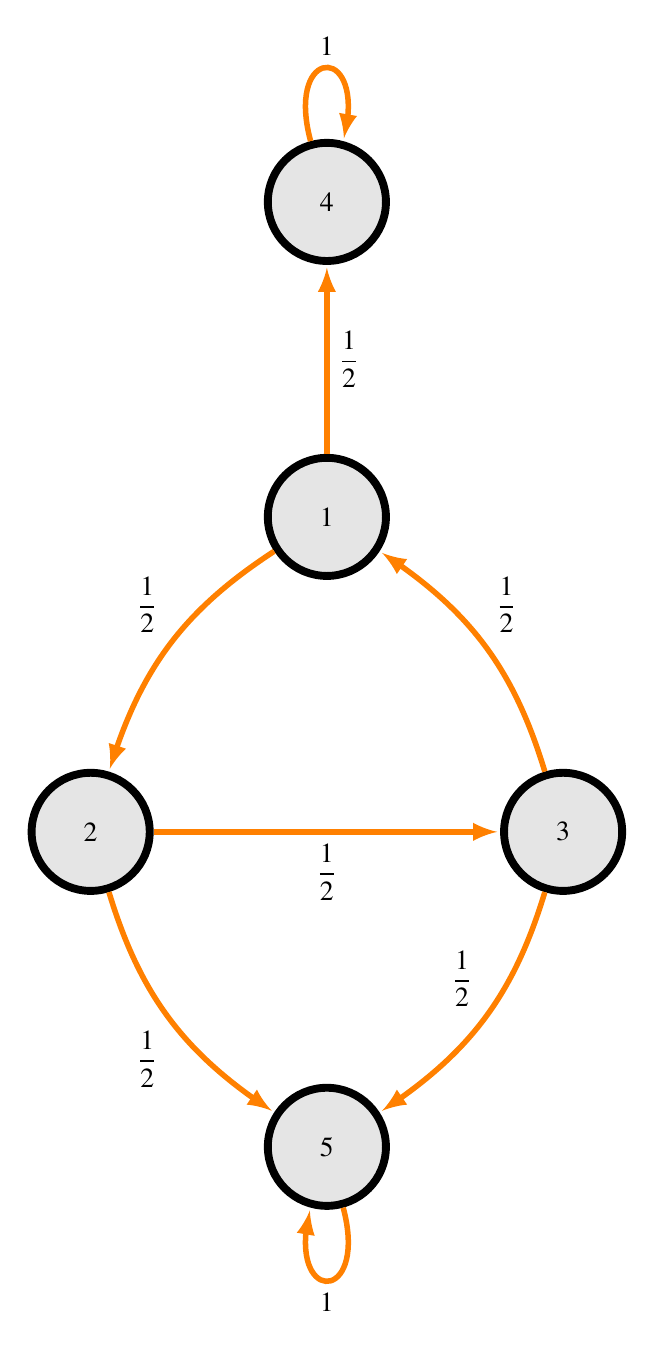
\begin{tikzpicture}
    % Setup the style for the states
        \tikzset{node style/.style={state, 
                                    minimum width=1.5cm,
                                    line width=1mm,
                                    fill=gray!20!white}}
        % Draw the states
        \node[node style] at (3, -4)      (bull)     {1};
        \node[node style] at (0, -8)      (bear)     {2};
        \node[node style] at (6, -8) (stagnant) {3};
        \node[node style] at (3, 0) (over1) {4};
        \node[node style] at (3, -12) (over2) {5};
        % Connect the states with arrows
        \draw[every loop,
              auto=right,
              line width=0.7mm,
              >=latex,
              draw=orange,
              fill=orange]
            (stagnant)     edge[bend right=20]            node {$\dfrac{1}{2}$} (bull)
            (stagnant)     edge[bend left=20]            node {$\dfrac{1}{2}$} (over2)
            (bull)     edge[bend right=20] node {$\dfrac{1}{2}$} (bear)
            (bull)     edge node {$\dfrac{1}{2}$} (over1)
            (bear)     edge[bend right=20] node {$\dfrac{1}{2}$} (over2)
            (bear)     edge node {$\dfrac{1}{2}$} (stagnant)
            (over1) edge[loop above]             node  {1} (over1)
            (over2) edge[loop below]             node  {1} (over2);
\end{tikzpicture}
\end{figure}
%

%\item Consider a Markov Chain with state space $\cbrak{0,1,2}$ and transition matrix
%\begin{align}
%P = 
%\begin{blockarray}{c@{\hspace{1pt}}rrr@{\hspace{3pt}}}
%         & 0   & 1   & 2 \\
%        \begin{block}{r@{\hspace{3pt}}@{\hspace{1pt}}
%    (@{\hspace{1pt}}rrr@{\hspace{1pt}}@{\hspace{1pt}})}
%        0 & \frac{1}{2} & \frac{1}{2} & 0  \\
%        1 & 0 &\frac{1}{2}  & \frac{3}{4}  \\
%%
%        2 &  \frac{1}{3} & \frac{1}{3} & \frac{1}{3}  \\
%        \end{block}
%    \end{blockarray}
%\end{align}
%For any two states $i$ and $j$, let $p_{ij}^{(n)}$ denote the $n$-step transition probability of going from $i$ to $j$.  Identify correct statements.
%\begin{enumerate}
%\item $\lim_{n \to \infty} p_{11}^{(n)} = \frac{2}{9}$
%\item $\lim_{n \to \infty} p_{21}^{(n)} = 0$
%\item $\lim_{n \to \infty} p_{32}^{(n)} = \frac{1}{3}$
%\item $\lim_{n \to \infty} p_{13}^{(n)} = \frac{1}{3}$
%\end{enumerate}

\end{enumerate}

% \section{June 2016}
% \renewcommand{\theequation}{\theenumi}
\renewcommand{\thefigure}{\theenumi}
\begin{enumerate}[label=\thesection.\arabic*.,ref=\thesection.\theenumi]
\numberwithin{equation}{enumi}
\numberwithin{figure}{enumi}
\numberwithin{table}{enumi}
\item The joint probability density function of (X,Y) is
\begin{equation}
    f(x,y) =
    \begin{cases}
        6(1-x) & if \hspace{0.3cm}0<y<x ,0<x<1\label{0.0.1} \\
        0      & \text{otherwise}
    \end{cases}
\end{equation}
Which among the following are correct?
\begin{enumerate}\itemsep0.3cm
    \item X and Y are not independent
    \item
          $ f_Y(y) =
              \begin{cases}
                  3\brak{y-1}^{2} & if \hspace{0.3cm}0<y<1 \\
                  0               & \text{otherwise}
              \end{cases}$
    \item X and Y are independent
    \item $ f_Y(y) =
              \begin{cases}
                  3\brak{\displaystyle{y-\frac{1}{2}{y}^2}} & if \hspace{0.3cm}0<y<1 \\
                  0                                         & \text{otherwise}
              \end{cases}$
\end{enumerate}
%
\solution
Given joint probability density function of X and Y, marginal probability density functions are as follows:
\begin{align}
    f_X(x) = \int_{-\infty}^{\infty} f(x,y) dy \\[0.4cm]
    f_Y(y) = \int_{-\infty}^{\infty} f(x,y) dx
\end{align}
Calculating $f_X(x)$
\begin{align}
    f_X(x) = & \int_{-\infty}^{\infty} f(x,y) dy \\
    =        & \int_{0}^{x} 6(1-x) dy            
\end{align}
\begin{align}
    f_X(x) =
    \begin{cases}
        6x(1-x) & 0<x<1     \label{june2016-104:0.0.6}\\
        0       & otherwise
    \end{cases}
\end{align}
Calculating $f_Y(y)$
\begin{align}
    f_Y(y) = & \int_{-\infty}^{\infty} f(x,y) dx \\
    =        & \int_{y}^{1} 6(1-x) dx\\
    =        & 6x -3{x}^2 \big|_{y}^{1}\\
    =        & 3 - 6y + 3y^{2}\\
    =        & 3{(y-1)}^{2}      
\end{align}
\begin{align}
    f_Y(y) =
    \begin{cases}
        3{(y-1)}^{2}  & 0<y<1     \label{june2016-104:0.0.12}\\
        0       & otherwise
    \end{cases}
\end{align}
To check whether X and Y are independent, we calculate $f_X(x) \times f_Y(y)$. From \eqref{june2016-104:0.0.6} and \eqref{june2016-104:0.0.12}
\begin{align}
    f_X(x) \times f_Y(y) = &
    \begin{cases}
        18x(1-x){(y-1)}^{2}  \\ \hspace{1.2cm}0<x<1,0<y<1\\
        0 \hspace{1cm} \text{otherwise}
    \end{cases}\\
    \neq & f(x,y)
\end{align}
Since f(x,y) and $f_X(x)\times f_Y(y)$ are different, random variables X and Y are not independent.
\begin{center}
    Options 1 and 2 are correct
\end{center}
%
\item Three types of components are used in electrical circuits 1, 2, 3 as shown below in the figure
\begin{figure}[h]
    \centering
    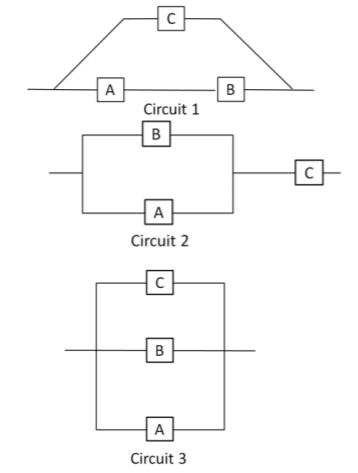
\includegraphics[width=\columnwidth]{solutions/2016/june/118/Figures/circuits.png}
    \caption{Figure}
    \label{fig:fig_label}
\end{figure}
%
\solution
For $q_1$, the truth table
\begin{table}[h]
    \centering
    \begin{tabular}{|c|c|c|c|}
    \hline
         $A$ & $B$ & $C$ & $(AB) + C$ \\
         \hline
         1 &1  & 0 &1\\\hline
         1&1&1&1\\\hline
         0&1&1&1\\\hline
         0&0&1&1\\\hline
         1&0&1&1\\
    \hline
    \end{tabular}
    \caption{Circuit 1 working}
    \label{june2016-118:tab:my_label}
\end{table}
Multiplying and adding probability for each case of $q_1$ gives us the value of $q_1$ as
\begin{align}
    q_1 = p^3-2p^2+1
\end{align}
For $q_2$, the truth table
\begin{table}[h]
    \centering
    \begin{tabular}{|c|c|c|c|}
    \hline
         $A$ & $B$ & $C$ & $(A+B)C$ \\
         \hline
         1&1&1&1\\ \hline
         1&0&1&1\\\hline
         0&1&1&1\\
    \hline
    \end{tabular}
    \caption{Circuit 2 working}
    \label{june2016-118:tab:table2}
\end{table}
Multiplying and adding probability for each case of $q_2$ gives us the value of $q_2$ as
\begin{align}
    q_2 = p^3-p^2-p+1
\end{align}
For $q_3$, the truth table
\begin{table}[h]
    \centering
    \begin{tabular}{|c|c|c|c|}
    \hline
         $A$ & $B$ & $C$ & $A + B + C$ \\
         \hline
         1&0&0&1\\\hline
         0&1&0&1\\\hline
         0&0&1&1\\\hline
         1&1&0&1\\\hline
         1&0&1&1\\\hline
         0&1&1&1\\\hline
         1&1&1&1\\
    \hline
    \end{tabular}
    \caption{Circuit 3 working}
    \label{june2016-118:tab:table3}
\end{table}
Multiplying and adding probability for each case of $q_3$ gives us the value of $q_3$ as
\begin{align}
    q_3 = 1-p^3
\end{align}
%%
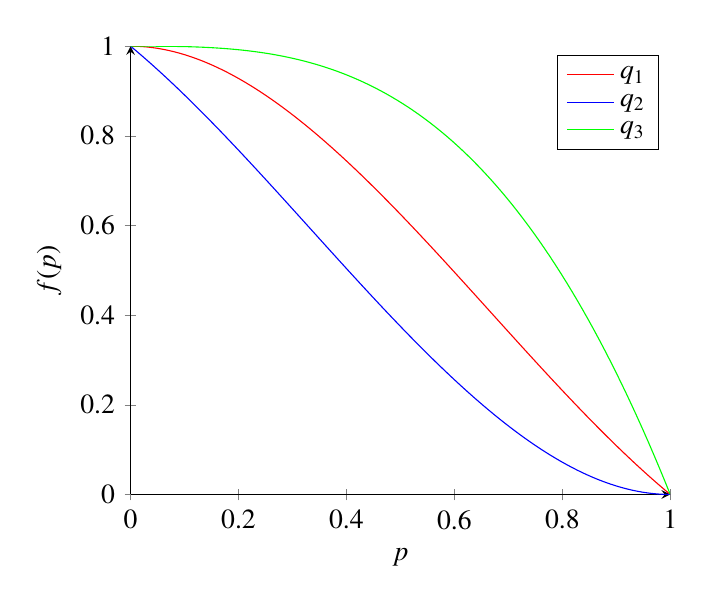
\begin{tikzpicture}
\begin{axis}[
    axis lines = left,
    xlabel = $p$,
    ylabel = {$f(p)$},
]
\addplot [
    domain=0:1, 
    samples=100, 
    color=red,
]
{x^3-2*x^2+1};
\addlegendentry{$q_1$}
\addplot [
    domain=0:1, 
    samples=100, 
    color=blue,
    ]
    {x^3-x^2-x+1};
\addlegendentry{$q_2$}
\addplot [
    domain=0:1, 
    samples=100, 
    color=green,
]
{1-x^3};
\addlegendentry{$q_3$}
\end{axis}
\end{tikzpicture}
\begin{align}
    \therefore q_3>q_1>q_2
\end{align}
Hence \textbf{Option 1} is correct


\end{enumerate}
% \section{December 2015}
% \renewcommand{\theequation}{\theenumi}
\renewcommand{\thefigure}{\theenumi}
\begin{enumerate}[label=\thesection.\arabic*.,ref=\thesection.\theenumi]
\numberwithin{equation}{enumi}
\numberwithin{figure}{enumi}
\numberwithin{table}{enumi}

\item The probability that a ticketless traveler is caught during a trip is 0.1. If the traveler makes 4 trips , the probability that he/she will be caught during at least one of the trips is:\\
\begin{enumerate}
    \item $1-(0.9)^4$
    \item $(1-0.9)^4$
    \item $1-(1-0.9)^4$
    \item $(0.9)^4$
\end{enumerate}
\solution
Let $X_i\in\cbrak{0,1}$ represent the ith trip where 1 denotes a ticketless traveller is caught.
Given,
\begin{align}
     \pr{X_i=1}&=p=0.1 \label{dec2015-3:a}
\end{align}
Let,
\begin{align}
    X=\sum_{i=1}^n X_i
\end{align}
where n is the number of trips and X has a binomial distribution.
\begin{align}
    p_X(k)&=
    \begin{cases}
     \comb{n}{k}\,p^K(1-p)^{n-k}, & 0\le k\le n
     \\
    0, & otherwise
    \end{cases}\label{dec2015-3:z}
\end{align}
As he/she makes 4 trips in total, Using \eqref{dec2015-3:a} and
\eqref{dec2015-3:z},
\begin{align}
    \pr{X=0}&=p_X(0)\\
    &=\comb{4}{0}\,p^0(1-p)^4\\
    \pr{X=0}&=(0.9)^4\label{dec2015-3:2}
\end{align}
Then probability of being caught in atleast one trip is,(Using \eqref{dec2015-3:2})
\begin{align}
    \pr{X\ge1}&=1-\pr{X<1}\\
    &=1-\pr{X=0}\label{dec2015-3:1}\\
    &=1-(0.9)^4
\end{align}

\item Suppose that $(X,Y)$ has a joint probability distribution with the marginal distribution of $X$ being N(0,1) and $E(Y|X=x)=x^3$ for all $x \in R$. Then, which of the following statements are true?
\begin{enumerate}
    \item Corr$(X,Y) = 0$
    \item Corr$(X,Y) > 0$
    \item Corr$(X,Y) < 0$
    \item X and Y are independent
\end{enumerate}
\solution
The following result shall be useful later. For $n \in N$
\begin{align}
    \int_{-\infty}^{\infty} \dfrac{x^n e^{\frac{-x^2}{2}}}{\sqrt{2\pi}}dx = 
    \begin{cases}
    0 & n\; is\; odd\\
    (n-1)\times...\times3\times1 & n\; is\; even
    \end{cases}
\end{align}
The proof for the above can be found at the end of the solution.
\begin{align}
    Corr(X,Y) = \cfrac{\sigma_{XY}^2}{\sigma_X\sigma_Y}
    \label{dec2015-108:correlationofxy}
\end{align}
We know $X \sim N(0,1)$. Thus,
\begin{align}
    f_X(x) &= \dfrac{e^{\frac{-x^2}{2}}}{\sqrt{2\pi}}\\
    E(X) &= 0\\
    \sigma_X^2 &= 1
\end{align}
\begin{align}
    \sigma_Y^2 = E(Y^2) - E(Y)^2
    \label{dec2015-108:varianceofy}
\end{align}
\begin{align}
    E(Y) &= \int_{-\infty}^{\infty}E(Y|X=x)f_X(x)dx\\
         &= \int_{-\infty}^{\infty}\dfrac{x^3 e^{\frac{-x^2}{2}}}{\sqrt{2\pi}}dx\\
         &= 0
\end{align}
\begin{align}
    E(Y^2) &= \int_{-\infty}^{\infty}E(Y^2|X=x)f_X(x)dx\\
           &= \int_{-\infty}^{\infty}\dfrac{x^6 e^{\frac{-x^2}{2}}}{\sqrt{2\pi}}dx\\
           &= 15
\end{align}
Substituting in \eqref{dec2015-108:varianceofy}
\begin{align}
    \sigma_Y^2 = 15
\end{align}
\begin{align}
    \sigma_{XY}^2 = E(XY) - E(X)E(Y)
    \label{dec2015-108:covarianceofxy}
\end{align}
\begin{align}
    E(XY) &= \int_{-\infty}^{\infty}E(XY|X=x)f_X(x)dx\\
          &= \int_{-\infty}^{\infty}E(xY|X=x)f_X(x)dx\\
          &= \int_{-\infty}^{\infty}xE(Y|X=x)f_X(x)dx\\
          &= \int_{-\infty}^{\infty}\dfrac{x^4 e^{\frac{-x^2}{2}}}{\sqrt{2\pi}}dx\\
          &= 3
\end{align}
Substituting in \eqref{dec2015-108:covarianceofxy}
\begin{align}
    \sigma_{XY}^2 = 3
\end{align}
Substituting in \eqref{dec2015-108:correlationofxy}
\begin{align}
    Corr(X,Y) = \cfrac{3}{\sqrt{15}} > 0
\end{align}
Since $Corr(X,Y) \ne 0$, X and Y are dependent. Thus option 2 is the only correct option.
\textbf{Proof for the integral:}
If n is odd, $\dfrac{x^n e^{\frac{-x^2}{2}}}{\sqrt{2\pi}}$ is an odd function, thus
\begin{align}
    \int_{-\infty}^{\infty} \dfrac{x^n e^{\frac{-x^2}{2}}}{\sqrt{2\pi}}dx = 0
\end{align}
If n is even, 
\begin{align}
    \int_{-\infty}^{\infty} \dfrac{x^n e^{\frac{-x^2}{2}}}{\sqrt{2\pi}}dx = \int_{-\infty}^{\infty} (x^{n-1}) (\dfrac{x e^{\frac{-x^2}{2}}}{\sqrt{2\pi}})dx
\end{align}
Using integration by parts,
\begin{multline}
    \int_{-\infty}^{\infty} \dfrac{x^n e^{\frac{-x^2}{2}}}{\sqrt{2\pi}}dx = \left(x^{n-1}\int \dfrac{x e^{\frac{-x^2}{2}}}{\sqrt{2\pi}}dx\right)\biggr \vert_{-\infty}^{\infty}\\
       - (n-1)\int_{-\infty}^{\infty}x^{n-2}\left(\int \dfrac{x e^{\frac{-x^2}{2}}}{\sqrt{2\pi}}dx\right) dx
\end{multline}
\begin{align}
    &= \left(x^{n-1}(-\dfrac{e^{\frac{-x^2}{2}}}{\sqrt{2\pi}})\right)\biggr \vert_{-\infty}^{\infty}
           - (n-1)\int_{-\infty}^{\infty}x^{n-2}(-\dfrac{e^{\frac{-x^2}{2}}}{\sqrt{2\pi}}) dx\\
    &= (n-1)\int_{-\infty}^{\infty} \dfrac{x^{n-2} e^{\frac{-x^2}{2}}}{\sqrt{2\pi}}dx\\
    &= (n-1)(n-3)\int_{-\infty}^{\infty} \dfrac{x^{n-4} e^{\frac{-x^2}{2}}}{\sqrt{2\pi}}dx\\
    &= (n-1)\times...\times3\times1\int_{-\infty}^{\infty} \dfrac{x^0 e^{\frac{-x^2}{2}}}{\sqrt{2\pi}}dx\\
    &= (n-1)\times...\times3\times1
\end{align}
%
 \item Let $X_1,X_2,...,X_n$ be independent and identically distributed, each having a uniform distribution on $(0,1)$. Let $S_n=\sum_{i=1}^{n}X_i$ for $n\ge 1$. Then, which of the following statements are true? 
\begin{enumerate}[label=\Alph*)]
\item $\frac{S_n}{n \log{n}}\to 0 \text{ as } n \to \infty$ with probability 1.
\item $\pr{\brak{S_n>\frac{2n}{3}}\text{occurs for infinitely many n}}=1$
\item $\frac{S_n}{\log{n}}\to 0\text{ as } n \to \infty$ with probability 1.
\item $\pr{\brak{S_n>\frac{n}{3}}\text{occurs for infinitely many n}}=1$
\end{enumerate}
%
\solution
\begin{table}[htp]
\centering
    \resizebox{\columnwidth}{20mm}{
\begin{tabular}{ |c|c|c|} 
\hline
\textbf{Symbol} & \textbf{expression/definition} \\
\hline
$S_n$ & $\displaystyle \sum_{i=1}^{n}X_i$  \\
\hline
$\mu_n$ & $\displaystyle \frac{1}{n} \sum_{i=1}^{n}X_i$  \\
\hline
& Independent continuous random\\$X$&variable identical to $X_1,X_2,...,X_n$ \\
\hline
\end{tabular}}
\caption{Variables and their definitions}
\label{dec2015-106:table1}
\end{table}
\begin{enumerate}
\item 
Given
\begin{align}
\displaystyle S_n=\sum_{i=1}^{n}X_i , n\ge 1
\end{align}
Dividing by $n$ on both sides
\begin{align}
\dfrac{S_n}{n}=\displaystyle\frac{1}{n} \sum_{i=1}^{n}X_i=\mu_n
\end{align}
It can be said that $X_1,X_2,...,X_n$ are the trials of $X$. By definition
\begin{align}
E\sbrak{X}&=\displaystyle \lim_{n\to \infty} \frac{\sum_{i=1}^{n}X_i}{n}=\lim_{n\to \infty} \frac{S_n}{n}\\
&\lim_{n\to \infty} \frac{S_n}{n}=E\sbrak{X}=\frac{1}{2} \label{dec2015-106:eq:mu_value} \\
\therefore&\lim_{n\to \infty} \frac{S_n}{n\log{n}}=0
\end{align}
\item
Using weak law, \eqref{dec2015-106:eq:mu_value}, and table \eqref{dec2015-106:table1}
\begin{align}
\lim_{n\to\infty} \pr{\abs{\mu_n-E\sbrak{X}}>\epsilon}=0, \forall \epsilon >0\\
\displaystyle \lim_{n\to\infty} \pr{S_n=\frac{n}{2}}=1 \label{dec2015-106:eq:weak_law}
\end{align}
It can be easily implied from \eqref{dec2015-106:eq:weak_law} that option B is false.
\item 
It is easy to observe from \eqref{dec2015-106:eq:mu_value} that option C is false.
\item
Using \eqref{dec2015-106:eq:weak_law}, we get
\begin{align}
\pr{\brak{S_n>\frac{n}{3}}\text{occurs for infinitely many n}}=1
\end{align}
\end{enumerate}
%
\item A fair coin is tossed repeatedly. Let $X$ be the number of tails before the first heads occurs. Let $Y$ denote the number of tails between the first and second heads. Let $X+Y = N$. Then which of the following are true?
\begin{enumerate}
    \item X and Y are independent random variables with
    {\footnotesize
    \begin{align}
        \pr{X = k} = \pr{Y = k} =
        \begin{cases}
            2^{-(k+1)} & k=0,1,2 \ldots
            \\
            0 & otherwise
        \end{cases}
    \end{align}
    }
    \item $N$ has a probability mass function given by
    {\small
     \begin{align}
        \pr{N = k} =
        \begin{cases}
            (k-1)2^{-k} & k=2,3,4 \ldots
            \\
            0 & otherwise
        \end{cases}
    \end{align}
    }
    \item Given $N = n$, the conditional distribution of X and Y are independent
    \item Given $N = n$
     \begin{align}
        \pr{X = k} =
        \begin{cases}
            \frac{1}{n+1} & n=0,1,2 \ldots
            \\
            0 & otherwise
        \end{cases}
    \end{align}
\end{enumerate}
%
\item An urn has 3 red and 6 black balls. Balls are drawn at random one by one without replacement. The probability that second red ball appears on fifth draw is: \\
\begin{enumerate}
    \item $\frac{1}{9!}$
    \newline
    \item $\frac{4!}{9!}$
    \newline
    \item $4\brak{\frac{6!4!}{9!}}$
    \newline
    \item $\frac{6!4!}{9!}$
\end{enumerate}
%
%
\solution
 To obtain a second red ball at the fifth draw, the first 4 trials should involve drawing only 1 red ball out of the 3 and 3 black balls out of the 6. Probability of this happening:
 \begin{align}
  \frac{\comb{3}{1}\comb{6}{3}}{\comb{9}{4}}
     \end{align}
The probability of the fifth ball turning out to be red is:
\begin{align}
    \frac{\comb{2}{1}}{\comb{5}{1}}
\end{align}
By Multiplication rule, total probability:
\begin{align}
    \frac{\comb{3}{1}\comb{6}{3}\comb{2}{1}}{\comb{5}{1}\comb{9}{4}}
    = \frac{3!\times 6!\times2!\times4!\times4!\times5!}{2!\times3!\times3!\times5!\times9!}\\ 
    =4\brak{\frac{4!6!}{9!}}
\end{align}

%
\item Let $X_i 's$ be independent random variables such that $X_i 's$ are symmetric about 0 and $var(X_i)=2i - 1$,for $i\geq 1$.then,
$\lim_{n \to \infty}\pr{X_1 +X_2 + \dots + X_n > n\log{n}}$
\begin{enumerate}
\begin{multicols}{2}
\setlength\itemsep{2em}
\item does not exist.
\item equals $\dfrac{1}{2}$.\\
\item equals 1.
\item equals 0.
\end{multicols}
\end{enumerate}
%
\solution
Let $X= X_1 +X_2 + \dots + X_n $,
as $X_i 's$ are symmetric about 0.
The mean of X is given by,
\begin{align}
E[X]=0 \label{dec2015-53:a}
\end{align}
the variance of X is given by,
\begin{align}
var[X]&= \sum_{i=1}^{n}(2i -1)\\
   &= \frac{2n(n+1)}{2} - n\\
   &= n^{2}
\end{align}
the standard deviation,
\begin{align}
\sigma_X = n \label{dec2015-53:b}
\end{align}
Applying Chebyshev's Inequality for the random variable X, for any $k>0$
\begin{align}
\pr{\abs{X-E[X]}> k\sigma_X} \leq \frac{1}{k^{2}} \label{dec2015-53:c}
\end{align}
let $k=\log{n} $ ,
using \eqref{dec2015-53:a} and \eqref{dec2015-53:b} in \eqref{dec2015-53:c},
\begin{align}
\pr{\abs{X}> n\log{n}} \leq \frac{1}{(\log{n})^{2}}\\
\pr{X> n\log{n}} + \pr{X< -n\log{n}} \leq \frac{1}{(\log{n})^{2}} \label{dec2015-53:e}
\end{align}
As, X is symmetric about 0,
\begin{align}
\pr{X> n\log{n}} =\pr{X< -n\log{n}} \label{dec2015-53:f}
\end{align}
using \eqref{dec2015-53:f} in \eqref{dec2015-53:e},
\begin{align}
2\pr{X> n\log{n}} \leq \frac{1}{(\log{n})^{2}}\\
\pr{X> n\log{n}} \leq \frac{1}{2(\log{n})^{2}}
\end{align}
as any probability is greater than 0,
\begin{align}
0< \pr{X> n\log{n}} \leq \frac{1}{2(\log{n})^{2}} \label{dec2015-53:d}
\end{align}
applying sandwich principle to \eqref{dec2015-53:d},
\begin{align}
\lim_{n \to \infty} 0< \lim_{n \to \infty} \pr{X> n\log{n}} \leq \lim_{n \to \infty} \frac{1}{2(\log{n})^{2}}\\
\lim_{n \to \infty}\pr{X_1 +X_2 + \dots + X_n > n\log{n}} = 0
\end{align}
Hence the option.4 is correct.
%
\item Suppose
$\begin{pmatrix}
X\\
Y
\end{pmatrix}$ is a random vector such that the marginal distribution of $X$ and the marginal distribution of $Y$ are the same and each is normally distributed with mean 0 and variance 1. Then, which of the following conditions imply independence of $X$ and $Y?$
\begin{enumerate}
\item Cov$\brak{X,Y}=0$
\item $aX+bY$ is normally distributed with mean 0 and variance $a^2+b^2$ for all real $a$ and $b$
\item $\pr{X\le 0, Y\le0}=\frac{1}{4}$
\item $E\sbrak{e^{itX+isY}}=E\sbrak{e^{itX}}E\sbrak{e^{isY}}$ for all real $s$ and $t$
\end{enumerate}
%
\solution


An important property of dirac delta function that will be used at multiple ocassions in this solution is
\begin{align}
\displaystyle\int\limits_{-\infty}^{\infty} f(x)\delta(x-a)dx=f(a) \label{dec/2015/109/eq:dirac}
\end{align}
Given $X\sim N\brak{0,1}, Y\sim N(0,1)$
\begin{enumerate}
\item
\begin{align}
Cov(X,Y)=0\\
E\sbrak{XY}-E\sbrak{X}E\sbrak{Y}=0\\
E\sbrak{XY}=0\\
\displaystyle \int\limits_{-\infty}^{\infty} \int\limits_{-\infty}^{\infty}xyf_{XY}(x,y) dxdy=0
\end{align}
This doesn't imply independence. Counter example given below\\
Lets consider a case where $X$ and $Y$ are dependent based on the following relation, $Y$ being independent of $K$
\begin{align}
X=KY \label{dec/2015/109/eq:case}
\end{align}
PMF for $K$ is given as
\begin{align}
p_K(k)=
\begin{cases}
\frac{1}{2} &k=1\\
\frac{1}{2} & k=-1\\
0 & \text{otherwise}
\end{cases}
\end{align}
A simulation is given below, Y is gaussian, then X also follows gaussian
\begin{figure}[!ht]
\centering
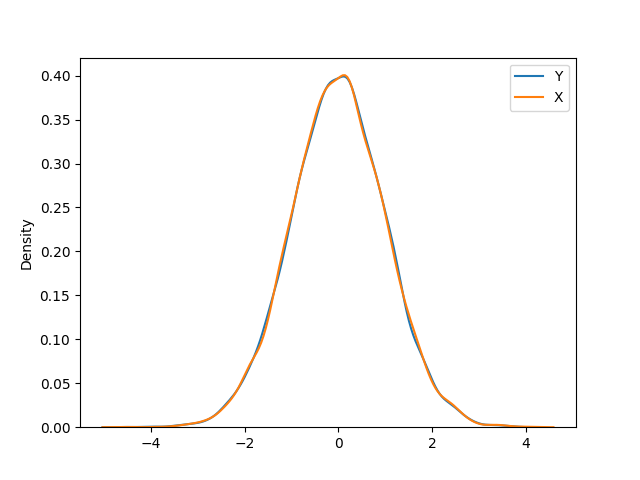
\includegraphics[width=\columnwidth]{solutions/2015/dec/109/figure/fig.png}
\caption{X and Y, if Y is normal}
\label{fig:dec/2015/109/plot}
\end{figure}
Theoretically it can be proved in the following manner,
Since $K$ and $Y$ are independent
\begin{align}
f_X(x)&=\pr{K=1}f_Y(x)+\pr{K=-1}f_Y(-x)\\
&=\frac{1}{2}\brak{f_Y(x)+f_Y(-x)}\\
&=f_Y(x)
\end{align}
Therefore, $X$ follows identical but not independent distribution as $Y$, An alternative proof is given below as a proof for marginal probability\\
Now consider that $X$ is normally distributed, we will establish $Y$ is also normally distributed.
The joint probability distribution is therefore
\begin{align}
f_{XY}(x,y)&=f_{X|Y}(x|y)f_X(x)\nonumber \\
&=f_X(x)\frac{1}{2}(\delta(x+y)+\delta(x-y))\label{dec/2015/109/eq:counter}
\end{align}
The marginal probability distribution function for $X$ is given as
\begin{align}
\int\limits_{-\infty}^{\infty}f_X(x)\frac{1}{2}(\delta(x+y)+\delta(x-y)) dy
\end{align}
Using \eqref{dec/2015/109/eq:dirac}, we get
\begin{align}
\int\limits_{-\infty}^{\infty}f_X(x)\frac{1}{2}(\delta(x+y)+\delta(x-y))dy=f_X(x)
\end{align}
We know that $X\sim N(0,1)$, $f_X(x)$ represents gaussian probability distribution function.\\
Futher, using symmetry of \eqref{dec/2015/109/eq:case}, we can establish that marginal distribution of $Y$ is gaussian. Here is a proof anyways
\begin{align}
f_Y(y)=\int\limits_{-\infty}^{\infty}f_X(x)\frac{1}{2}(\delta(x+y)+\delta(x-y)) dx
\end{align}
Using \eqref{dec/2015/109/eq:dirac}, we get
\begin{align}
f_Y(y)=\frac{1}{2}\brak{f_X(y)+f_X(-y)}=f_X(y)
\end{align}
Since $Y$ has identical probability distribution function, $Y\sim N(0,1)$\\
The covariance is given as
\begin{align}
&Cov(X,Y)=E[XY]-E[X]E[Y]=E[XY]\\
&E[XY]=\int\limits_{-\infty}^{\infty}\int\limits_{-\infty}^{\infty}xyf_{XY}(x,y) dy dx
\end{align}
\begin{align}
=\int\limits_{-\infty}^{\infty}\int\limits_{-\infty}^{\infty}xyf_X(x)\frac{1}{2}(\delta(x+y)+\delta(x-y)) dy dx\\
=\int\limits_{-\infty}^{\infty} xf_X(x)\int\limits_{-\infty}^{\infty}y\frac{1}{2}(\delta(x+y)+\delta(x-y)) dy dx
\end{align}
Using \eqref{dec/2015/109/eq:dirac}
\begin{align}
E[XY]=\int\limits_{-\infty}^{\infty}xf_X(x)\frac{1}{2}(x-x)dx=0
\end{align}
\item
Defining the following matrices/vectors
\begin{table}[h!]
\centering
\begin{tabular}{ |c|c|} 
\hline
\textbf{vector/matrix} & \textbf{expression} \\
\hline&\\[-1em]
$\boldsymbol{Z}$& $\begin{pmatrix} X &Y\end{pmatrix}^\top$\\[2pt]
\hline&\\[-1em]
$\boldsymbol{C}$&$\begin{pmatrix} a &b\end{pmatrix}^\top$  \\[2pt]
\hline&\\[-1em]
$\boldsymbol{\mu}$&$\begin{pmatrix} 0 &0\end{pmatrix}^\top$  \\[2pt]
\hline&\\[-1em]
$\boldsymbol{\Sigma}$&$\begin{pmatrix}1&\rho\\\rho&1\end{pmatrix}$ \\
\hline
\end{tabular}
\caption{vectors/matrices and their expressions}
\label{dec/2015/109/table1}
\end{table}
Given
\begin{align}
\boldsymbol{C^\top Z}\sim N\brak{0,a^2+b^2}
\end{align}
Since this is true for all $a$ and $b$, it is equivalent to $X$ and $Y$ being jointly gaussian
\begin{align}
\boldsymbol{Z}\sim N(\boldsymbol{\mu},\boldsymbol{\Sigma})
\end{align}
For correlated random variables $X$ and $Y$ in bivariate normal distribution, we have
\begin{align}
\sigma_{Z}^2=\displaystyle\sum_{i,j}\Sigma_{ij}\\
a^2+b^2=a^2+b^2+2\rho ab\\
\therefore \rho=0\label{dec/2015/109/eq:rho}
\end{align}
The joint distribution is given as
\begin{align}
f_{\boldsymbol{Z}}(x,y)=\frac{\text{exp}\brak{-\frac{1}{2}\brak{\boldsymbol{z-\mu}}^\top\boldsymbol{\Sigma}^{-1}\brak{\boldsymbol{z-\mu}}}}{\sqrt{(2\pi)^2\abs{\boldsymbol{\Sigma}}}}\\
f_{\boldsymbol{Z}}(x,y)=\frac{\text{exp}\brak{-\frac{1}{2}{\begin{pmatrix} x &y\end{pmatrix}} I_2{\begin{pmatrix} x &y\end{pmatrix}}^\top}}{\sqrt{(2\pi)^2}}
\end{align}
Where $I_2$ is the identity matrix of order 2
\begin{align}
f_{\boldsymbol{Z}}(x,y)=\frac{\text{exp}\brak{-\frac{1}{2}{\begin{pmatrix} x &y\end{pmatrix}} {\begin{pmatrix} x &y\end{pmatrix}}^\top}}{\sqrt{(2\pi)^2}}\\
f_{\boldsymbol{Z}}(x,y)=\frac{\text{exp}\brak{-\frac{1}{2}\brak{x^2+y^2}}}{\sqrt{(2\pi)^2}}=f_X(x)f_Y(y)
\end{align}
$\therefore$ \textbf{Option(2) is correct}, A simulation for bivariate gaussian is given below
\begin{figure}[!ht]
\centering
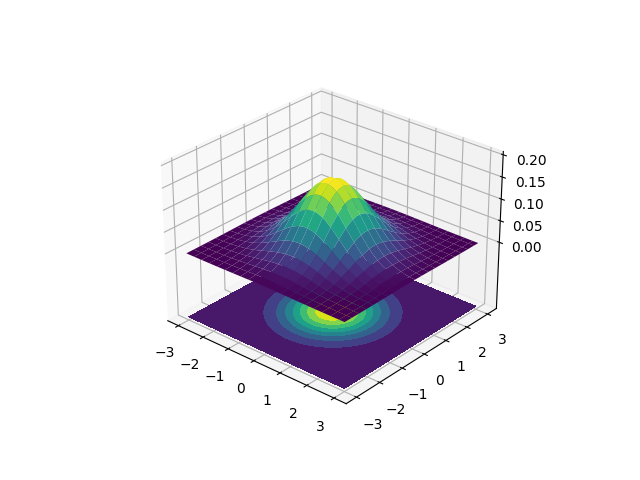
\includegraphics[width=\columnwidth]{solutions/2015/dec/109/figure/plot.png}
\caption{bivariate gaussian while 0 mean vector and identity covariance matrix}
\label{dec/2015/109/plot}
\end{figure}
\item
\begin{align}
\pr{X\le 0, Y\le0}=\frac{1}{4}
\end{align}
This doesn't imply independence, it can be true even for dependent $X$ and $Y$, the counter example is \eqref{dec/2015/109/eq:counter}, the joint probability function is symmetric across all 4 quadrants
\begin{align}
\therefore \pr{X\le 0, Y\le0}=\frac{1}{4}
\end{align}
Alternatively, here is proof 
\begin{align}
\pr{X\le 0}=F_X(0)=\frac{1}{2} \label{dec/2015/109/eq:pr1}
\end{align}
Using \eqref{dec/2015/109/eq:case}
\begin{align}
\pr{Y\le 0|X\le 0}=\frac{1}{2} \label{dec/2015/109/eq:pr2}
\end{align}
Using \eqref{dec/2015/109/eq:pr1} and \eqref{dec/2015/109/eq:pr2}
\begin{align}
\pr{X\le 0, Y\le0}=\frac{1}{4}
\end{align}
\item
\begin{align}
E\sbrak{e^{itX+isY}}=E\sbrak{e^{itX}}E\sbrak{e^{isY}}\\
E\sbrak{e^{itX+isY}}=\varphi_X(t)\varphi_Y(s) \label{dec/2015/109/eq:inde}
\end{align}
The inverse is given as
\begin{align}
f_{XY}(x,y)=\frac{1}{4\pi^2}\displaystyle \int\limits_{-\infty}^{\infty} \int\limits_{-\infty}^{\infty} e^{-itX-isY}E\sbrak{e^{itX+isY}}ds dt
\end{align}
Using \eqref{dec/2015/109/eq:inde}
\begin{align}
f_{XY}(x,y)&=\frac{1}{4\pi^2}\displaystyle \int\limits_{-\infty}^{\infty} \int\limits_{-\infty}^{\infty} e^{-itX-isY}\varphi_X(t)\varphi_Y(s) ds dt\\
&f_{XY}(x,y)=f_X(x)f_Y(y)
\end{align}
$\therefore$ \textbf{Option(4) is correct}
\end{enumerate}




\end{enumerate}

% \section{June 2015}
% \renewcommand{\theequation}{\theenumi}
\renewcommand{\thefigure}{\theenumi}
\begin{enumerate}[label=\thesection.\arabic*.,ref=\thesection.\theenumi]
\numberwithin{equation}{enumi}
\numberwithin{figure}{enumi}
\numberwithin{table}{enumi}

\item Let $\vec{A}$,$\vec{B}$ be n × n matrices.Which of the following equals trace$(\vec{A}^2 \vec{B}^2)$?\\

\begin{enumerate}
\item (trace$(\vec{A} \vec{B}))^2.$
\item trace$(\vec{A} \vec{B}^2 \vec{A}).$
\item trace$((\vec{A} \vec{B})^2).$
\item trace$(\vec{B} \vec{A} \vec{B} \vec{A}).$
\end{enumerate}
%
%
%
\solution
See Table \ref{eq:solutions/2015/june/27/Table1:}

\onecolumn
\begin{longtable}{|p{5cm}|p{13cm}|}
\hline
\textbf{Statement} &\textbf{Solution}\\
\hline
Definition & The trace of an n × n square matrix $\vec{A}$ is defined as:
\begin{displaymath}tr({\vec{A}}) = \sum_{i=1}^n a_{ii} \end{displaymath}

where $a_{ii}$ denotes the entry on the ith row and ith column of $\vec{A}.$ \\
\hline
Properties&
\parbox{12cm}{\begin{align}\text{The properties of the trace}:
tr(c{\vec{A}})=c\;tr({\vec{A}})\\
tr({\vec{A}}^T)=tr({\vec{A}})\\
tr({\vec{A}}+{\vec{B}})=tr({\vec{B}}+{\vec{A}})\\
tr({\vec{A}}{\vec{B}})=tr({\vec{B}}{\vec{A}})\label{eq:solutions/2015/june/27/eq}\\
tr({\vec{A}}^T{\vec{B}})=tr({\vec{A}}{\vec{B}}^T)\\
tr({\vec{R}}^{-1}{\vec{A}}{\vec{R}})=tr({\vec{R}}^{-1}({\vec{A}}{\vec{R}}))\\
=tr(({\vec{A}}{\vec{R}}){\vec{R}}^{-1})=tr({\vec{A}})
\end{align}}\\
\hline
Checking $tr$$(\vec{A}^2 \vec{B}^2).$ &
\parbox{12cm}{\begin{align}
 \text{Upon rewriting and from \eqref{eq:solutions/2015/june/27/eq}, } tr(\vec{A}^2 \vec{B}^2)=tr(\vec{A}\vec{A} \vec{B}\vec{B})\\
           = tr(\vec{B}\vec{A} \vec{A}\vec{B})\\
           = tr(\vec{B}\vec{B} \vec{A}\vec{A})\\
           = tr(\vec{A}\vec{B} \vec{B}\vec{A})\label{eq:solutions/2015/june/27/eq1}\\
           = tr(\vec{A}\vec{A} \vec{B}\vec{B})\\
           = tr(\vec{A}^2 \vec{B}^2)\label{eq:solutions/2015/june/27/eq2}
\end{align}}\\
\hline
Checking ($tr$$(\vec{A} \vec{B}))^2.$&
\parbox{12cm}{\begin{align}\text{from \eqref{eq:solutions/2015/june/27/eq},}\
    (tr(\vec{A} \vec{B}))^2=(tr(\vec{B} \vec{A}))^2
\end{align}}\\
\hline
 Checking $tr$$(\vec{A} \vec{B}^2 \vec{A}).$&
\parbox{12cm}{\begin{align}\text{Rewriting,}
\  tr(\vec{A} \vec{B}^2 \vec{A}) =tr(\vec{A}\vec{B} \vec{B}\vec{A})\\\text{ from \eqref{eq:solutions/2015/june/27/eq},}\
 tr(\vec{A} \vec{B}^2 \vec{A})=  tr(\vec{A}\vec{A} \vec{B}\vec{B})\label{eq:solutions/2015/june/27/eql}=tr(\vec{A}^2 \vec{B}^2)  
\end{align}}\\
\hline
Checking $tr$$(\vec{A} \vec{B})^2.$&
\parbox{12cm}{\begin{align}\text{from \eqref{eq:solutions/2015/june/27/eq},}\
 tr(\vec{A} \vec{B})^2=tr(\vec{B}\vec{A})^2 
\end{align}}\\
\hline
 Checking $tr$$(\vec{B} \vec{A} \vec{B} \vec{A}).$&
\parbox{12cm}{\begin{align}\text{from \eqref{eq:solutions/2015/june/27/eq}}\\
 tr(\vec{B} \vec{A} \vec{B} \vec{A}) =tr(\vec{A}\vec{B} \vec{A}\vec{B})\\
 =tr(\vec{B}\vec{A} \vec{B}\vec{A})
 \end{align}}\\
\hline
 Conclusion&
Hence, from \eqref{eq:solutions/2015/june/27/eq}, and \eqref{eq:solutions/2015/june/27/eql} option 2, ie  $tr$$(\vec{A} \vec{B}^2 \vec{A}).$ is the correct answer.\\
\hline
\caption{Solution}
\label{eq:solutions/2015/june/27/Table1:}
\end{longtable}
\twocolumn

\item The row space of a $20 \times 50$ matrix $\vec{A}$ has dimension 13.What is the dimension of the space of solution $\vec{Ax}=0$?
\begin{enumerate}
\item{7}
\item{13}
\item{33}
\item{37}
\end{enumerate}
%
%
\solution
See Table \ref{eq:solutions/2015/june/29/table1}

\begin{table*}[ht!]
\begin{center}
\begin{tabular}{|c|c|}
\hline
\textbf{Options} & \textbf{Explanation} \\
\hline
\text{7} & \\
Given & A:$\vec{R^{50}}\rightarrow \vec{R^{20}}$ is a linear transformation\\
& $dim$(row space($\vec{A}$))=$rank$($\vec{A}$)=13\\
Rank Nullity Theorem& $\vec{A}$:$\vec{R^{50}}\rightarrow \vec{R^{20}}$ is a linear transformation then,\\
& $rank$($\vec{A}$)+$nullity$($\vec{A}$)=50\\
& 13 + $nullity$($\vec{A}$)=50\\
& $nullity$($\vec{A}$)=37\\
& $dim$(space of solution($\vec{Ax}=0$))=$nullity$($\vec{A}$)=37\\
& Hence,incorrect\\
\hline\\
\text{13} & 
From above,it is obvious that it is incorrect\\
\hline
\text{33}
& It is also incorrect.\\
\hline
\text{37}
& From above it is correct\\

\hline
\end{tabular}
\end{center}
\caption{Finding Correct Option}
\label{eq:solutions/2015/june/29/table1}
\end{table*}
 

\item Given a $4 \times 4$ matrix $\vec{A}$, let $T:\mathbb R^4 \rightarrow \mathbb R^4$ be the linear transformation defined by $\vec{T}\vec{v} = \vec{A}\vec{v}$, where we think of $\mathbb R^4$ as the set of real $4 \times 1$ matrices. For which choices of $\vec{A}$ given below, do Image$(\vec{T})$ and Image$(\vec{T}^2)$ have respective dimensions 2 and 1? ($*$ denotes a nonzero entry)
\begin{enumerate}
    \item $\vec{A} = \myvec{0 & 0 & * & * \\ 0 & 0 & * & * \\ 0 & 0 & 0 & * \\ 0 & 0 & 0 & 0}$
    \item $\vec{A} = \myvec{0 & 0 & * & 0 \\ 0 & 0 & * & 0 \\ 0 & 0 & 0 & * \\ 0 & 0 & 0 & *}$
    \item $\vec{A} = \myvec{0 & 0 & 0 & 0 \\ 0 & 0 & 0 & 0 \\ 0 & 0 & 0 & * \\ 0 & 0 & * & 0}$
    \item $\vec{A} = \myvec{0 & 0 & 0 & 0 \\ 0 & 0 & 0 & 0 \\ 0 & 0 & * & * \\ 0 & 0 & * & *}$
\end{enumerate}
%
%
\solution
We can say,
\begin{align}
    \vec{T}(\vec{v}) = \vec{A}\vec{v} = \text{Image}(\vec{T}) = C(\vec{A})\\
    \vec{T}^2(\vec{v}) = \vec{A}^2\vec{v} = \text{Image}(\vec{T}^2) = C(\vec{A}^2)
\end{align}
where $C(\vec{A})$ and $C(\vec{A}^2)$ denote the columnspace of $\vec{A}$ and $\vec{A}^2$ respectively. Therefore,
\begin{align}
    \text{dimension}(\text{Image}(\vec{T})) = \text{dimension}(C(\vec{A})) = \text{rank}(\vec{A})\\
    \text{dimension}(\text{Image}(\vec{T}^2)) = \text{dimension}(C(\vec{A}^2)) = \text{rank}(\vec{A}^2)
\end{align}
See Table     \ref{eq:solutions/2015/june/31/tab:proof}

\onecolumn
\begin{longtable}{|l|l|}
    \hline
        & \\
        1. $\vec{A} = \myvec{0 & 0 & * & * \\ 0 & 0 & * & * \\ 0 & 0 & 0 & * \\ 0 & 0 & 0 & 0}$ & The number of linearly independent columns in $\vec{A}$ is 2\\
    \hline
        & \\
        & hence, $dim(Image(\vec{T})) = dim(C(\vec{A})) = 2$\\
        & \\
        & $\vec{A}^2 = \myvec{0 & 0 & 0 & * \\ 0 & 0 & 0 & * \\ 0 & 0 & 0 & 0 \\ 0 & 0 & 0 & 0}$\\
        & \\
        & The number of linearly independent columns in $\vec{A}^2$ is 1\\
        & hence, $dim(Image(\vec{T}^2)) = dim(C(\vec{A}^2)) = 1$\\
        & \\
        & $\therefore$ This option is true.\\
    \hline
        & \\
        2. $\vec{A} = \myvec{0 & 0 & * & 0 \\ 0 & 0 & * & 0 \\ 0 & 0 & 0 & * \\ 0 & 0 & 0 & *}$ & The number of linearly independent columns in $\vec{A}$ is 2\\
        & hence, dim(Image($\vec{T}$)) = dim(C($\vec{A}$)) = 2\\
        & \\
        & $\vec{A}^2 = \myvec{0 & 0 & 0 & * \\ 0 & 0 & 0 & * \\ 0 & 0 & 0 & * \\ 0 & 0 & 0 & *}$\\
        & \\
        & The number of linearly independent columns in $\vec{A}^2$ is 1\\
        & hence, dim(Image($\vec{T}^2$)) = dim(C($\vec{A}^2$)) = 1\\
        & \\
        & $\therefore$ This option is true.\\
    \hline
        & \\
        3. $\vec{A} = \myvec{0 & 0 & 0 & 0 \\ 0 & 0 & 0 & 0 \\ 0 & 0 & 0 & * \\ 0 & 0 & * & 0}$ & The number of linearly independent columns in $\vec{A}$ is 2\\
        & hence, $dim(Image(\vec{T})) = dim(C(\vec{A})) = 2$\\
        & \\
        & $\vec{A}^2 = \myvec{0 & 0 & 0 & 0 \\ 0 & 0 & 0 & 0 \\ 0 & 0 & * & 0 \\ 0 & 0 & 0 & *}$\\
        & \\
        & The number of linearly independent columns in $\vec{A}^2$ is 2\\
        & hence, $dim(Image(\vec{T}^2)) = dim(C(\vec{A}^2)) = 2 \neq 1$\\
        & \\
        & $\therefore$ This option is false.\\
    \hline
        & \\
        4. $\vec{A} = \myvec{0 & 0 & 0 & 0 \\ 0 & 0 & 0 & 0 \\ 0 & 0 & * & * \\ 0 & 0 & * & *}$ & This option is false\\
        & Counter example:\\
        & For some non-zero $b,c \in \mathbb R$, let\\
        & $\vec{A} = \myvec{0 & 0 & 0 & 0 \\ 0 & 0 & 0 & 0 \\ 0 & 0 & b & b \\ 0 & 0 & c & c}$\\
        & \\
        & The number of linearly independent columns in $\vec{A}$ is 1\\
        & hence, $dim(Image(\vec{T})) = dim(C(\vec{A})) = 1 \neq 2$\\
        & \\
    \hline
    \caption{Verifying with the options}
    \label{eq:solutions/2015/june/31/tab:proof}
\end{longtable}
\twocolumn

\item %
Let $\vec{F}:\mathbb{R}^n\times\mathbb{R}^n\rightarrow\mathbb{R}$ be the function $\vec{F}(\vec{x},\vec{y})=\langle\vec{Ax},\vec{y}\rangle$, where $\langle,\rangle$ is the standard inner product of $\mathbb{R}^n$ and $\vec{A}$ is a $n\times n$ real matrix. Here D denotes the total derivative. Which of the following statements are correct?
\begin{enumerate}
    \item $(D\vec{F}(\vec{x},\vec{y}))(\vec{u},\vec{v})=\langle\vec{Au},\vec{y}\rangle+\langle\vec{Ax},\vec{v}\rangle$.
    \item $(D\vec{F}(\vec{x},\vec{y}))(0,0)=0$.
    \item $D\vec{F}(\vec{x},\vec{y})$ may not exist for some $(\vec{x},\vec{y})\in\mathbb{R}^n\times\mathbb{R}^n$.
    \item $D\vec{F}(\vec{x},\vec{y})$ does not exist at $(\vec{x},\vec{y})=(0,0)$.
\end{enumerate}
%
%
\solution
See Tables \ref{eq:solutions/2015/june/68/deftab}, \ref{eq:solutions/2015/june/68/obs}
and \ref{eq:solutions/2015/june/68/sol}

\onecolumn
\begin{longtable}{|l|l|}
\hline
\endhead
\textbf{Inner product}&Inner product between two vectors $\vec{x}$ and $\vec{y}$ is defined as\\&\parbox{13cm}{\begin{align}
    \langle\vec{x},\vec{y}\rangle=\vec{x}^T\vec{y}\label{eq:solutions/2015/june/68/inp}
\end{align}}\\&Where $\vec{x}$,$\vec{y}\in\mathbb{R}^n$\\
\hline
\textbf{Inner Product}&\\\textbf{Property used}&\parbox{13cm}{\begin{align}
    \langle\vec{x},\vec{y}\rangle=\vec{x}^T\vec{y}=\vec{y}^T\vec{x}=\langle\vec{y},\vec{x}\rangle\label{eq:solutions/2015/june/68/prop1}
    \end{align}}\\
\hline
\textbf{Total Derivative} $D$&Total derivative is a linear transformation. For function $\vec{F}(\vec{x},\vec{y})$, the total\\& derivative is given as $D\vec{F}(\vec{x},\vec{y})$ which says that total derivative of\\&function $\vec{F}$ at $(\vec{x},\vec{y})$.\\
\hline
\caption{Definitions and theorem used}
\label{eq:solutions/2015/june/68/deftab}
\end{longtable}
\begin{longtable}{|l|l|}
\hline
\endhead
\textbf{Statement}&\textbf{Observations}\\
\hline
Given&Function $\vec{F}:\mathbb{R}^n\times\mathbb{R}^n\rightarrow\mathbb{R}$, it is given as\\&\parbox{13cm}{\begin{align}
    \vec{F}(\vec{x},\vec{y})=\langle\vec{Ax},\vec{y}\rangle=\vec{x}^T\vec{A}^T\vec{y}\label{eq:solutions/2015/june/68/F}
\end{align}}\\&where $\vec{x}$,$\vec{y}\in\mathbb{R}^n$\\&Using property \eqref{eq:solutions/2015/june/68/prop1}, we can also get\\&\parbox{13cm}{\begin{align}
    \implies\vec{F}(\vec{x},\vec{y})=\langle\vec{y},\vec{Ax}\rangle\\
    \implies\vec{F}(\vec{x},\vec{y})=\vec{y}^T\vec{A}\vec{x}\label{eq:solutions/2015/june/68/Fp}
\end{align}}\\
\hline
Total Derivative $D$&Now we will calculate $D\vec{F}(\vec{x},\vec{y})$\\&\parbox{13cm}{\begin{align}
    D\vec{F}(\vec{x},\vec{y})=\myvec{\frac{\partial \vec{F}}{\partial \vec{x}}&\frac{\partial \vec{F}}{\partial \vec{y}}}\label{eq:solutions/2015/june/68/D}
\end{align}}\\&From \eqref{eq:solutions/2015/june/68/F},\eqref{eq:solutions/2015/june/68/Fp} we get\\&\parbox{13cm}{\begin{align}
    \frac{\partial \vec{F}}{\partial \vec{x}}=\vec{y}^T\vec{A}\label{eq:solutions/2015/june/68/df1}\\
    \frac{\partial \vec{F}}{\partial \vec{y}}=\vec{x}^T\vec{A}^T\label{eq:solutions/2015/june/68/df2}
\end{align}}\\&Substitute \eqref{eq:solutions/2015/june/68/df1} and \eqref{eq:solutions/2015/june/68/df2} in \eqref{eq:solutions/2015/june/68/D}\\&\parbox{13cm}{\begin{align}
    D\vec{F}(\vec{x},\vec{y})=\myvec{\vec{y}^T\vec{A}&\vec{x}^T\vec{A}^T}_{1\times n^2}\label{eq:solutions/2015/june/68/Dsol}
\end{align}}\\
\hline
\caption{Observations}
\label{eq:solutions/2015/june/68/obs}
\end{longtable}
\begin{longtable}{|l|l|l|}
\hline
\endhead
\textbf{Option}&\textbf{Solution}&\textbf{True/}\\&&\textbf{False}\\
\hline
1&First we calculate $(D\vec{F}(\vec{x},\vec{y}))(\vec{u},\vec{v})$ where $\vec{u}$,$\vec{v}\in\mathbb{R}^n$&\\&Using \eqref{eq:solutions/2015/june/68/Dsol}and block matrix multiplication we get&\\&\parbox{14cm}{\begin{align}
    (D\vec{F}(\vec{x},\vec{y}))(\vec{u},\vec{v})=\myvec{\vec{y}^T\vec{A}&\vec{x}^T\vec{A}^T}\myvec{\vec{u}\\\vec{v}}\\
    \implies(D\vec{F}(\vec{x},\vec{y}))(\vec{u},\vec{v})=\vec{y}^T\vec{A}\vec{u}+\vec{x}^T\vec{A}^T\vec{v}\label{eq:solutions/2015/june/68/eq1}\\
    (D\vec{F}(\vec{x},\vec{y}))(\vec{u},\vec{v})=\langle\vec{y},\vec{Au}\rangle+\langle\vec{Ax},\vec{v}\rangle
\end{align}}&\\&Using property \eqref{eq:solutions/2015/june/68/prop1} we get&True\\&\parbox{14cm}{\begin{align}
    (D\vec{F}(\vec{x},\vec{y}))(\vec{u},\vec{v})=\langle\vec{Au},\vec{y}\rangle+\langle\vec{Ax},\vec{v}\rangle\label{eq:solutions/2015/june/68/p1}
\end{align}}&\\
\hline
2.&Using \eqref{eq:solutions/2015/june/68/eq1}, if $\vec{u}=0$ and $\vec{v}=0$ then we get&\\&\parbox{14cm}{\begin{align}
    (D\vec{F}(\vec{x},\vec{y}))(0,0)=0\label{eq:solutions/2015/june/68/p2}
\end{align}}&True\\
\hline
3.&Since from \eqref{eq:solutions/2015/june/68/Dsol} we can say that $D\vec{F}(\vec{x},\vec{y})$ will exist for any $(\vec{x},\vec{y})\in\mathbb{R}^n\times\mathbb{R}^n$.&False\\&&\\
\hline
4.&From \eqref{eq:solutions/2015/june/68/Dsol}, if $(\vec{x},\vec{y})=(0,0)$ we get&\\&\parbox{14cm}{\begin{align}
    D\vec{F}(\vec{x},\vec{y})|_{(0,0)}=0
\end{align}}&\\&Therefore we can say that $D\vec{F}(\vec{x},\vec{y})$ will exist at $(\vec{x},\vec{y})=(0,0)$.&False\\
\hline
\caption{Solution}
\label{eq:solutions/2015/june/68/sol}
\end{longtable}
\twocolumn

\item 	%
	An $n\times n$ complex matrix $\vec{A}$ satisfies $\vec{A}^{k} = \vec{I}_n$. the $n\times n$ identity matrix, where $k$ is a positive integer $>$ 1. Suppose 1 is not an eigenvalue of $\vec{A}$. Then which of the following statements are necessarily true?\\
	
	\begin{enumerate}
		\item $\vec{A}$ is diagonalizable. \\
		\item $\vec{A}+\Vec{A}^2+...+\vec{A}^{k-1} = 0$, the $n\times n$ zero matrix. \\
		\item $tr(\vec{A})+tr(\Vec{A}^2)+...+tr(\vec{A}^{k-1}) = -n$ \\
		\item $\vec{A}^{-1}+\Vec{A}^{-2}+...+\vec{A}^{-(k-1)} = -\vec{I}_n$
	\end{enumerate}
%
%
\solution
See Tables \ref{eq:solutions/2015/june/70/tab1}
and \ref{eq:solutions/2015/june/70/tab2}
\onecolumn
	\begin{longtable}{|l|l|}
		\hline
		\multirow{3}{*}{Minimal Polynomial} 
		& \\
		& The minimal polynomial $\mu_{\vec{A}}$ of an $n\times n$ matrix $\vec{A}$ over a field $\mathbf{F}$ is the \\
		& monic polynomial $P$ over the field $\mathbf{F}$ of least degree such that $P(\Vec{A}) = 0$. Any \\
		& other polynomial $Q$ with $Q(\vec{A}) = 0$ is polynomial multiple of $\mu_{\vec{A}}$. \\
		& \\
		\hline
		\multirow{3}{*}{Eigen Value and } 
		& \\
		& If $\lambda$ is an eigen value of matrix $\Vec{A}$ then $\lambda$ will also be the root of the minimal \\ Minimal Polynomial
		& polynomial $\mu_{\vec{A}}$.\\
		& \\
		\hline
		\multirow{3}{*}{Diagonalizability and} 
		& \\
		& If $\Vec{A}$ is an $n\times n$ matrix with $n$ distinct eigenvalues, then $\vec{A}$ is diagonalizable \\ Eigen Values
		& \\
		\hline
		\multirow{3}{*}{Polynomial and} 
		& \\
		& If a polynomial is of form $x^{k}-1$, it can be written as \\ it's Zeros
		& \\
		& \qquad \qquad \qquad $x^{k}-1$ = $(x - 1)(1 + x + x^2 + ... + x^{k-1})$\\
		& \\
		& The zeros to the given polynomial will be of the format \\
		& \\
		& \qquad \qquad \qquad $e^{\frac{n2\pi i}{k}}$ \qquad for $0 \leq n < k$. \\
		& \\
		& From this we can see that all the roots of the equation $x^{k}-1$ will be distinct. \\
		& \\
		\hline
	\end{longtable}
	\begin{longtable}{|l|l|}
		\hline
		\multirow{3}{*}{Inference from }   
		& \\ 
		& We are given that \\the Given Data
		& \\
		& \qquad \qquad \qquad$\vec{A}^k = \vec{I}_n$ \\
		& \\
		& This can be written as \\
		& \\
		& \qquad \qquad \qquad$\vec{A}^k - \vec{I}_n = 0$ \\
		& \\
		& This resembles the polynomial equation of the form $x^{k}-1$, So we further write \\
		& the above equation as \\
		& \\
		& \qquad \qquad $\implies \vec{A}^k - \vec{I}_n = 0$ \\
		& \\
		& \qquad \qquad $\implies (\vec{A} - \vec{I}_n)(\vec{I}_n + \vec{A} + \vec{A}^2 + ... + \vec{A}^{k-1}) = 0$ \\
		& \\
		& Let $\mu_{\vec{A}}$ be the minimal polynomial of $\vec{A}$. \\
		& It is given that 1 is not an eigenvalue of $\vec{A}$. That means $\mu_{\vec{A}}$ cannot divide $(\vec{A} - \vec{I}_n)$.\\
		& \\
		& But $\mu_{\vec{A}}$ will be able to divide  $(\vec{I}_n + \vec{A} + \vec{A}^2 + ... + \vec{A}^{k-1})$ as it is a polynomial multiple of $\vec{A}$\\ 
		& \\
		& i.e. $(\vec{I}_n + \vec{A} + \vec{A}^2 + ... + \vec{A}^{k-1})$ is polynomial multiple of $\mu_{\vec{A}}$ \\
		& \\
		& \qquad \qquad  $\implies \vec{I}_n + \vec{A} + \vec{A}^2 + ... + \vec{A}^{k-1} = 0$ \\
		& \\
		& Since we know that $1 + x + x^2 + ... + x^{k-1}$ will have distinct roots which are not equal to 1. \\
		& \\
		\hline
		\multirow{3}{*}{Option 1  } & \\
		& We were able to find that $\implies \vec{I}_n + \vec{A} + \vec{A}^2 + ... + \vec{A}^{k-1}$ is a polynomial multiple of $\mu_{\vec{A}}$ \\
		& with $k-1$ distinct roots. Which implies that $\mu_{\vec{A}}$ will also have distinct roots. \\
		& \\
		& Since, there are distinct roots to the minimal polynomial, it implies that $\vec{A}$ will be \\ 
		& diagonalizable. \\
		& \\
		& $\therefore$ this statement is $\mathbf{True}$. \\
		&\\
		\hline
		\multirow{3}{*}{Option 2} & \\
		& We know that \\
		& \\
		& \qquad \qquad \qquad $\vec{I}_n + \vec{A} + \vec{A}^2 + ... + \vec{A}^{k-1} = 0$ \\
		& \\
		& \qquad \qquad $\implies \vec{A} + \vec{A}^2 + ... + \vec{A}^{k-1} = -\vec{I}_n$ \\
		& \\
		& $\therefore$ this statement is $\mathbf{False}$. \\
		&\\
		\hline
		\multirow{3}{*}{Option 3} & \\
		& We know that \\
		& \\
		& \qquad \qquad \qquad $\vec{I}_n + \vec{A} + \vec{A}^2 + ... + \vec{A}^{k-1} = 0$ \\
		& \\
		& \qquad \qquad $\implies \vec{A} + \vec{A}^2 + ... + \vec{A}^{k-1} = -\vec{I}_n$ \\
		& \\
		& Taking $trace()$ on both sides, we get \\
		& \\
		& \qquad \qquad $\implies tr(\vec{A} + \vec{A}^2 + ... + \vec{A}^{k-1}) = tr(-\vec{I}_n)$ \\
		& \\
		& \qquad \qquad $\implies tr(\vec{A}) + tr(\vec{A}^2) + ... + tr(\vec{A}^{k-1}) = tr(-\vec{I}_n)$ \qquad ($\because$ trace() is a linear function)\\
		& \\
		& \qquad \qquad $\implies tr(\vec{A}) + tr(\vec{A}^2) + ... + tr(\vec{A}^{k-1}) = -n$ \\
		& \\
		& $\therefore$ this statement is $\mathbf{True}$. \\
		&\\
		\hline
		\multirow{3}{*}{Option 4} & \\
		& We know that \\
		& \\
		& \qquad \qquad \qquad $\vec{I}_n + \vec{A} + \vec{A}^2 + ... + \vec{A}^{k-2} + \vec{A}^{k-1} = 0$ \\
		& \\
		& Multiply the whole equation with $\vec{A}^{-(k-1)}$. We get \\
		& \\
		& \qquad \qquad \qquad $\vec{A}^{-(k-1)} + \vec{A}^{1-(k-1)} + ... + \vec{A}^{k-2-(k-1)} + \vec{A}^{k-1-(k-1)} = 0$ \\
	    & \\
	    & \qquad \qquad $\implies \vec{A}^{-(k-1)} + \vec{A}^{1-(k-1)} + ... + \vec{A}^{-1} + \vec{I}_n = 0$ \\
	    & \\
	    & \qquad \qquad $\implies \vec{A}^{-1}+\Vec{A}^{-2}+...+\vec{A}^{-(k-1)} = -\vec{I}_n$ \\
	    & \\
		& $\therefore$ this statement is $\mathbf{True}$. \\
		&\\
		\hline
		\multirow{3}{*}{Conclusion} & \\
		& From our observation we see that \\
		&\\
		& Options 1), 3) and 4) are True.\\
		& \\
		\hline
\caption{}
\label{eq:solutions/2015/june/70/tab1}
	\end{longtable}
	\begin{longtable}{|l|l|}
		\hline
		\multirow{3}{*}{Complex Matrix }   
		& \\ 
		& Let the complex matrix $\vec{A}$ $=$ $\myvec{i&0 \\ 0&-i}$ \\ Example
		& \\
		& When $k = 4$, we get \\
		& \\
		& \qquad \qquad \qquad $\vec{A}^4 = \vec{I}_2$ \\
		& \\
		& \\
		& The eigen values of the matrix $\vec{A}$ are $-i$ and $+i$. \\
        & \\
        & Since, there are two distinct eigen values for the matrix $\vec{A}$,\\
        & $\vec{A}$ is diagonalizable. \\
        & \\
        & \\
        & Now checking the equation for $\vec{A}+\Vec{A}^2+...+\vec{A}^{k-1}$ \\
        & \\
        & \qquad \qquad \qquad $\vec{A}+\Vec{A}^2+\vec{A}^{3}$ \qquad ($\because$ here $k=4$) \\
        & \\
        & \qquad \qquad $\implies \myvec{i&0 \\ 0&-i} + \myvec{-1&0 \\ 0&-1} + \myvec{-i&0 \\ 0&i}$ \\
        & \\
        & \qquad \qquad $\implies \myvec{-1&0 \\ 0&-1} = -\vec{I}_2$  \\
        & \\
        & \\
        & Now checking the equation for $tr(\vec{A})+tr(\Vec{A}^2)+...+tr(\vec{A}^{k-1}) = -n$ \\
        & \\
        & \qquad \qquad \qquad $tr(\vec{A})+tr(\Vec{A}^2)+tr(\vec{A}^{3})$ \qquad ($\because$ here $k=4$) \\
        & \\
        & \qquad \qquad $\implies tr\myvec{i&0 \\ 0&-i} + tr\myvec{-1&0 \\ 0&-1} + tr\myvec{-i&0 \\ 0&i}$ \\
        & \\
        & \qquad \qquad $\implies 0+(-2)+0 = -2$\\
        & \\
		& \\
		& Now checking the equation for $\vec{A}^{-1}+\Vec{A}^{-2}+...+\vec{A}^{-(k-1)} = -\vec{I}_n$ \\
        & \\
        & \qquad \qquad \qquad $\vec{A}^{-1}+\Vec{A}^{-2}+\vec{A}^{-3}$ \qquad ($\because$ here $k=4$) \\
        & \\
        & \qquad \qquad $\implies \myvec{-i&0 \\ 0&i} + \myvec{-1&0 \\ 0&-1} + \myvec{i&0 \\ 0&-i}$ \\
        & \\
        & \qquad \qquad $\implies \myvec{-1&0 \\ 0&-1} = -\vec{I}_2$  \\
        & \\
		& \\
		\hline
\caption{}
\label{eq:solutions/2015/june/70/tab2}
	\end{longtable}
		
\twocolumn

\item Let $S$ be the set of 3x3 real matrices $\vec{A}$ with 
\begin{align}
    \vec{A}^T\vec{A}=\myvec{1&0&0\\0&0&0\\0&0&0}
\end{align}
Then the set contains:-\\
\begin{enumerate}
    \item a Nilpotent Matrix
    \item a matrix of rank one
    \item a matrix of rank two
    \item a non-zero skew symmetric matrix.
\end{enumerate}
%
%
\solution
See Tables     \ref{eq:solutions/2015/june/71/table:1}
and     \ref{eq:solutions/2015/june/71/table:2}.

\onecolumn
\begin{longtable}{|l|l|}
	\hline
	\multirow{3}{*}{Proof 1}	& \\
	&Let $\vec{A}x$=0 and $\mathbb{N(\vec{A})}$ is the null space of $\vec{A}$\\
	&\\
	$Rank(\vec{A})=Rank(\vec{A}^T\vec{A})$&Then $\vec{A}^T\vec{A}$x=0 which means $\mathbb{N(\vec{A})}\subset \mathbb{N(\vec{A}^T\vec{A})}$ \\
	&\\
	&Thus if $\vec{A}^T\vec{A}$x=0 ,then\\
	&\\
	&$x^T\vec{A}^T\vec{A}x=0\implies\lVert\vec{A}x\rVert=0$\\
	&\\
	&Which means $\vec{A}x=0$ thus\\
	&\\
	& $\mathbb{N(\vec{A}^T\vec{A})}\subset\mathbb{N(\vec{A})}$\\
	&\\
	&From the Above two condition we can say that ${N(\vec{A}^T\vec{A})}=\mathbb{N(\vec{A})}$\\
	&\\
	&$rank(\vec{A})=n-\mathbb{N(\vec{A})}$\\
	&\\
	&$rank(\vec{A})=rank(\vec{A}^T\vec{A})$\\
	&\\
	&Hence Proved.\\
	&\\
	\hline
	\multirow{3}{*}{Proof 2} 
	&\\
	&Suppose $\vec{A}=\myvec{\vec{a_1}&\hdots&\vec{a_n}}$ where $\vec{a_i}$ is the column vector of $\vec{A}$\\
	&\\
	Rowspace$(\vec{A}^T\vec{A})$=Rowspace($\vec{A}$) & $\vec{A}^T\vec{A}=\vec{A}^T\myvec{\vec{a_1}&\hdots&\vec{a_n}}=\myvec{\vec{A}^T\vec{a_1}&\hdots\vec{A}^T\vec{a_n}}$\\
	&\\
	&For each column of $\vec{A}^T\vec{A}$\\
	&\\
	&$\vec{A}^T\vec{a_i}=\myvec{\vec{b_1}&\hdots\vec{b_n}}\vec{a_i}$where $\vec{b_i}$ is the column vector of $\vec{A}^T$ and Row of $\vec{A}$\\
	&\\
	&$=\myvec{\vec{b_1}&\hdots\vec{b_n}}\myvec{a_{i1}\\ \vdots \\a_{in}}=\sum_{j=1}^{n}a_{ij}b_j$\\
	&\\
	&So column of $\vec{A}^T\vec{A}$ is the linear combination of rows of $\vec{A}$.\\
	&\\
	&Since rank$(\vec{A}^T)$=rank$(\vec{A})$ so,\\
	&\\
	&Row$(\vec{A}^T\vec{A})=$Column$(\vec{A}^T\vec{A})$=Row$(\vec{A})$\\
	&\\
	&Hence Proved.\\

	&\\
\hline
  
    \caption{Proofs}
    \label{eq:solutions/2015/june/71/table:1}
\end{longtable}
\begin{longtable}{|l|l|}
	\hline
	\multirow{3}{*}{Option 1} & \\
	&From Proof 2,Set $S$ contained a set of matrix whose First Column is Non-zero. \\ 
    & \\
    Nilpotent Matrix check&$S\in$ Set$\myvec{1&0&0\\0&0&0\\0&0&0}$,$\myvec{0&0&0\\1&0&0\\0&0&0}$,$\myvec{0&0&0\\0&0&0\\1&0&0}$\\
    &\\
    &Given $\vec{A}^T\vec{A}=\myvec{1&0&0\\0&0&0\\0&0&0}$\\
    &\\
    &So the only matrix $\vec{A}$ which satisfy $\vec{A}^T\vec{A}=\myvec{1&0&0\\0&0&0\\0&0&0}$, $\vec{A}^2=0$ such that $\vec{A}\in S$\\
    &\\
    &$\vec{A}=\myvec{0&0&0\\1&0&0\\0&0&0}\in S$\\
    &\\
    &$\vec{A}^T\vec{A}=\myvec{0&1&0\\0&0&0\\0&0&0}\myvec{0&0&0\\1&0&0\\0&0&0}=\myvec{1&0&0\\0&0&0\\0&0&0}$\\
    
    &\\
    &$\vec{A}^2=\myvec{0&0&0\\1&0&0\\0&0&0}\myvec{0&0&0\\1&0&0\\0&0&0}=\myvec{0&0&0\\0&0&0\\0&0&0}$ which is a nilpotent matrix\\
    &\\
    &Option 1 is correct.\\
    &\\
    \hline
	\multirow{3}{*}{Option 2}
	& \\
    &In Proof 1 we already prove that $Rank(\vec{A})=Rank(\vec{A}^T\vec{A})$\\
    &\\
    matrix of rank one check &Since the $Rank(\vec{A}^T\vec{A})=1$ so the $Rank(\vec{A})=1$ \\ 
	&\\
	&There fore Set S always contains only Rank 1 matrices.\\
	&\\
	&Hence Option 2 is correct.\\
	&\\
	\hline
	\multirow{3}{*}{Option 3}
	&\\
    &Since set S contain only rank 1 matrices and none of rank 2 matrices \\
    &\\
    matrix of rank two check&as already proved above therefore\\
    &\\
    &Option 3 is incorrect.\\
    &\\
    
    \hline
	\multirow{3}{*}{Option 4}
	&\\
	&Proved by contradiction\\
	&\\
    non-zero skew .&Assume Rank of $\vec{A}$ is 1 so $\vec{A}$ can be written as $\vec{A}=\vec{u}\vec{v}^T$ for any non-zero\\
    &\\
    symmetric matrix check&Columns vectors $\vec{u}$ , $\vec{v}$ with n entries. If A is skew symmetric,we have:-\\
    &\\
    &$\vec{A}^T=-\vec{A}$\\
    &\\
    &$(\vec{u}\vec{v})^T=-\vec{u}\vec{v}^T$ $\vec{v}\vec{u}^T=-\vec{u}\vec{v}^T$\\
    &\\
    &The Column space of these matrices is same.The column space of $\vec{v}\vec{u}^T$\\ 
    &is span of $\vec{v}$,where as the column space of $\vec{u}\vec{v}^T$ is the span of $\vec{u}$,\\
    &\\
    &So we must have $\vec{v}=k\vec{u}$ for some $k\in\mathbb{R}$.So the equation becomes\\
    &\\
    &$k\vec{u}\vec{u}^T=-k\vec{u}\vec{u}^T$ \\
    &\\
    &and since $\vec{u}\neq 0$;We can conclude that k=0,which means $\vec{v}=0$ therefore $\vec{A}=0$.\\
    &\\
    &This Contradicts our assumption that $\vec{A}$has rank 1.\\
    &\\
    &Thus real skew symmentric matrix can never have rank=1.\\
    &\\
    &Hence option 4 is incorrect.\\
    &\\
	\hline
	\multirow{3}{*}{Answers}
	&\\
&Option 1 and Option 2 are correct.\\
&\\
	\hline
	
	\caption{Solution Table}
    \label{eq:solutions/2015/june/71/table:2}
\end{longtable}
\twocolumn

\item Let $\vec{S}: \mathbb R^n \rightarrow \mathbb R^n$ be given by $\vec{S}(\vec{v}) = \alpha\vec{v}$, for a fixed $\alpha \in \mathbb R, \alpha \neq 0$. Let $\vec{T}: \mathbb R^n \rightarrow \mathbb R^n$ be a linear transformation such that $\vec{B} = \{ \vec{v}_1,\ldots,\vec{v}_n \}$ is a set of linearly independent eigenvectors of $\vec{T}$. Then
\begin{enumerate}
    \item The matrix of $\vec{T}$ with respect to $\vec{B}$ is diagonal
    \item The matrix of $(\vec{T}-\vec{S})$ with respect to $\vec{B}$ is diagonal
    \item The matrix of $\vec{T}$ with respect to $\vec{B}$ is not necessarily diagonal, but is upper triangular
    \item The matrix of $\vec{T}$ with respect to $\vec{B}$ is diagonal but the matrix of $(\vec{T}-\vec{S})$ with respect to $\vec{B}$ is not diagonal.
\end{enumerate}
%
\solution
Given that $\vec{T}: \mathbb R^n \rightarrow \mathbb R^n$ be a linear transformation and B represents a set of linearly independent eigenvectors of $\vec{T}$ given as follows
\begin{align}
    \vec{B} = \{\vec{v}_1,\ldots,\vec{v}_n\}
\end{align}
So,
\begin{align}
    \vec{T}(\vec{v}_i) = \vec{A}\vec{v}_i = \lambda_i\vec{v}_i
\end{align}
where $\lambda_i$ represents the eigenvalue corresponding to $\vec{v}_i$. Hence, the matrix $\vec{T}$ with respect to $\vec{B}$ can be represented as
\begin{align}
    [\vec{T}]_B = \myvec{\lambda_1 & 0 & \dots & 0\\ 0 & \lambda_2 & \dots & 0\\ \vdots & \ddots &  & \\ 0 & \dots & 0 & \lambda_n}\label{eq:solutions/2015/june/72/eq:T}
\end{align}
And,
\begin{align}
    (\vec{T}-\vec{S})\vec{v}_i & = \vec{T}(\vec{v}_i) - \vec{S}(\vec{v}_i)\\& = \lambda_i\vec{v}_i - \alpha\vec{v}_i \\ & = (\lambda_i - \alpha)\vec{v}_i
\end{align}
Hence, matrix of $\vec{T}-\vec{S}$ with respect to $\vec{B}$ can be represented as
\begin{align}
    [\vec{T}-\vec{S}]_B = \myvec{\lambda_1-\alpha & 0 & \dots & 0\\ 0 & \lambda_2-\alpha & \dots & 0\\ \vdots & \ddots &  & \\ 0 & \dots & 0 & \lambda_n-\alpha}\label{eq:solutions/2015/june/72/eq:T-S}
\end{align}
\onecolumn
\begin{longtable}{|l|l|}
    \hline
        & \\
        1. The matrix of $\vec{T}$ & True, as seen\\
        w.r.t to $\vec{B}$ is diagonal & from \eqref{eq:solutions/2015/june/72/eq:T}\\
        & \\
    \hline
        & \\
        2. The matrix of $(\vec{T}-\vec{S})$ & True, as seen\\
        w.r.t $\vec{B}$ is diagonal & from \eqref{eq:solutions/2015/june/72/eq:T-S}\\
        & \\
    \hline
        & \\
        3. The matrix of $\vec{T}$ with respect & False, as\\
        to $\vec{B}$ is not necessarily diagonal & already proved\\
        but is upper triangular & $[\vec{T}]_B$ is diagonal\\
        & \\
    \hline
        & \\
        4. The matrix of $\vec{T}$ with respect to $\vec{B}$ & False, as\\
        is diagonal but the matrix of $(\vec{T}-\vec{S})$ & already proved\\
        with respect to $\vec{B}$ is not diagonal & $[\vec{T}-\vec{S}]_B$\\
        & is diagonal\\
        & \\
    \hline
    \caption{Verifying the given options}
    \label{eq:solutions/2015/june/72/tab:proof}
\end{longtable}
\twocolumn
Let $T:\mathbb R^2 \rightarrow \mathbb R^2$ where
\begin{align}
    \vec{T}(x) = \vec{A}\vec{x} = \myvec{4 & -2 \\ 3 & -3}\myvec{x_1 \\ x_2}
\end{align}
Here, the eigenvalues of the above trasformation matrix are $\lambda_1 = 3, \lambda_2 = -2$. And the corresponding eigenvectors are $\vec{v}_1 = \myvec{2\\1}, \vec{v}_2 = \myvec{1\\3}$. Thus,
\begin{align}
    \vec{B} = \{ \vec{v}_1, \vec{v}_2 \}
\end{align}
Now,
\begin{align}
    \vec{T}(\vec{v}_1) & = \vec{A}\vec{v}_1\\&
    = \myvec{4 & -2 \\ 3 & -3}\myvec{2\\1} \\ &
    = \myvec{6\\3} \\&
    = 3\myvec{2\\1}\\&
    = \lambda_1\vec{v}_1
    \intertext{And,}
    \vec{T}(\vec{v}_2) & = \vec{A}\vec{v}_2\\&
    = \myvec{4 & -2 \\ 3 & -3}\myvec{1\\3} \\ &
    = \myvec{-2\\-6} \\&
    = -2\myvec{1\\3}\\&
    = \lambda_2\vec{v}_2\\
\end{align}
For any vector $\vec{v} \in \mathbb R^2, \vec{v} = c_1\vec{v}_1 + c_2\vec{v}_2$
\begin{align}
    [\vec{v}]_B = \myvec{c_1 \\ c_2}\\
    \vec{T}(\vec{v}) & = \vec{T}(c_1\vec{v}_1 + c_2\vec{v}_2)\\& = c_1\vec{T}(\vec{v}_1) + c_2\vec{T}(\vec{v}_2)\\ & = c_1\lambda_1\vec{v}_1 + c_2\lambda_2\vec{v}_2\\
    [\vec{T}(\vec{v})]_B & = \myvec{\lambda_1 c_1\\ \lambda_2 c_2} \\&
    = \myvec{\lambda_1 & 0 \\ 0 & \lambda_2}\myvec{c_1 \\ c_2} \\&
    = \myvec{\lambda_1 & 0 \\ 0 & \lambda_2} [\vec{v}]_B \\& = \myvec{3 & 0\\0&-2}[\vec{v}]_B \label{eq:solutions/2015/june/72/eq:finalT}\\
    \vec{S}(\vec{v}) & = \alpha\vec{v}, \alpha \neq 0\\&
    = \alpha(c_1\vec{v}_1 + c_2\vec{v}_2)\\&
    = \alpha c_1\vec{v}_1 + \alpha c_2\vec{v}_2
\end{align}
\begin{align}
    [\vec{S}(\vec{v})]_B = \myvec{\alpha c_1\\ \alpha c_2}\\
    [(\vec{T}-\vec{S})(\vec{v})]_B & = \myvec{\lambda_1 c_1 -\alpha c_1 \\ \lambda_2 c_2 -\alpha c_2}\\ & = \myvec{\lambda_1 -\alpha & 0 \\ 0 & \lambda_2 - \alpha}\myvec{c_1 \\ c_2}\\ &
    = \myvec{\lambda_1 -\alpha & 0 \\ 0 & \lambda_2 - \alpha}[\vec{v}]_B \\ & = \myvec{3 -\alpha & 0 \\ 0 & -2 - \alpha}[\vec{v}]_B \label{eq:solutions/2015/june/72/eq:finalT-S}
\end{align}
Hence, shown from \eqref{eq:solutions/2015/june/72/eq:finalT} and \eqref{eq:solutions/2015/june/72/eq:finalT-S} that the matrix of $\vec{T}$ and of $\vec{T}-\vec{S}$ w.r.t to $\vec{B}$ is diagonal.

\item Let $p_n\brak{x}=x^n$ for $x\in\mathbb{R}$ and let $\varrho=span\{p_0,p_1,p_2,...\}$. Then
\begin{enumerate}
    \item $\varrho$ is a vector space of all real valued continuous functions on $\mathbb{R}$.
    \item $\varrho$ is a subspace of all real valued continuous functions on $\mathbb{R}$.
    \item $\{p_0,p_1,p_2,...\}$ is a linearly independent set in the vector space of all real valued continuous functions on $\mathbb{R}$.
    \item Trigonometric functions belong to $\varrho$.
\end{enumerate}
%
%
\solution
See Table     \ref{eq:solutions/2015/june/74/tab:Ans}

\onecolumn
\begin{longtable}{|l|l|}
    \hline
    Given & $p_n\brak{x}=x^n$ for $x\in\mathbb{R}$ and $\varrho=span\{p_0,p_1,p_2,...\}$.\\
    \hline
    Vector& The set $S$ consisting of all real continuous functions on $\mathbb{R}$ forms a vector space.\\
    space&Let $f$ and $g$ be two real continuous functions from the set $S$.\\
    of real&Since the sum of two continuous function is a continuous function.\\
    continuous&$i)$ Addition is commutative $f+g=g+f$\\
    functions&$ii)$ Addition is associative$f+(g+h)=(f+g)+h$\\
    on $\mathbb{R}$&$iii)$There is unique $O$, zero function which maps every element to 0.\\
    &$iv)$Additive inverse.For each $f$ in $S$, $-f$ is a function in $S$.\\
    &$v)$Properties of scalar multiplication.For $c,c_1,c_2\in \mathbb{R}$,\\
    &\qquad $a)$ $1f=f$ where the constant function $1$ maps every element to $1$.\\
    &\qquad $b)$ $(c_1c_2)f=c_1(c_2f)$\\
    &\qquad $c)$ $c(f+g)=cf+cg$\\
    &\qquad $d)$ $c_1+c_2)f=c_1f+c_2f$\\
    &Hence the set $S$ forms a vector space.\\
    \hline
    Option 1& $\varrho$ represents the vector space of polynomials. Polynomial functions are infintely \\
    & continuously differentiable.So any function that is continuous but not differentiable can \\
    & not be represented by polynomials.\\
    & Example the function $\abs{x}$ is continous but cannot be represented in \\
    &polynomial basis.Therefore option 1 is incorrect.\\
    \hline
    Option 2& $\varrho$ forms a subspace of all real valued continuous function on $\mathbb{R}$\\
    &Let $\alpha,\beta$ be two polynomial functions of order m and n, represented by the tuple of\\ &coefficients $(a_0,a_2,a_2..a_m)$ and $(b_0,b_1,b_2...b_n)$,then $c\alpha+\beta$ is also\\
    & a polynomial function whose coefficients are $(ca_0+b_0,ca_1+b_1,ca_2+b_2...)$\\
    &Therefore $\varrho$ is a subspace of all real valued continuous functions on $\mathbb{R}$.\\
    & For example consider two functions $f=\{2,0,4\}$ and $g=\{0,2,1,5\}$,then $2f+g$ \\
    & will be $2f+g=2\brak{2+4x^2}+\brak{2x+x^2+5x^3}=4+2x+9x^2+5x^3=\{4,2,9,5\}$.\\
    \hline
    Option 3&Consider the expression\\
    &$a_0p_0+a_1p_1+a_2p_2+...=O\implies a_0=a_1=a_2=...=0$\\
    &Hence $\{p_0,p_1,p_2,..\}$ are linearly independent set in the vector space of all real valued \\
    &continuous functions on $\mathbb{R}$.\\
    \hline
    Option 4&The fundamental period of trigonometric functions is finite, where as polynomials are \\
    &aperiodic. So, they cannot belong to the same class.\\
    &For example $\sin{x}$ has a fundamental period of $2\pi$. $\tan{x}$ is continuous in the interval \\
    &$(-\frac{\pi}{2},\frac{\pi}{2})$, but is not defined at $k\frac{\pi}{2}$ where $k\in odd(\mathbb{N})$.\\
    \hline
    \caption{Answer}
    \label{eq:solutions/2015/june/74/tab:Ans}
\end{longtable}
\twocolumn

\item Which of the following are subspaces of the vector space $\mathbb{R}^3$?
\begin{enumerate}
  \item ${(x, y, z):x + y = 0}$
  \item ${(x, y, z):x - y = 0}$
  \item ${(x, y, z):x + y = 1}$
  \item ${(x, y, z):x - y = 1}$
\end{enumerate}
%
%
\solution
A subspace $\vec{S}$ of a vector space is defined as a non-empty subset that is closed under addition and scalar multiplication, i.e
\begin{enumerate}
  \item All possible linear combinations of the vectors in $\vec{S}$ lie in the subspace.
  \item Any vector in $\vec{S}$ scaled by a scalar $c$ lies in the subspace.
\end{enumerate}
We define any vector $\vec{V} \in \vec{S}$ for each of the subspaces defined in the options as:
\begin{align}
  \vec{V} = \myvec{x \\ y \\ z}
\end{align}

{Option 1:}
Let $\vec{A} = \myvec{x_1 \\ y_1 \\ z_1}$ and $\vec{B} = \myvec{x_1 \\ y_1 \\ z_2} \in \vec{S}$, and $k_1$ and $k_2$ be some scalars. As per definition:
\begin{align}
  \myvec{1 & 1 & 0}\vec{A} = \myvec{1 & 1 & 0}\vec{B} = 0
\end{align}
Verifying the property of the subspace by using the linear combination of $\vec{A}$ and $\vec{B}$:
\begin{multline}
    \myvec{1 & 1 & 0}\lcbrak{k_1\vec{A}} + \rcbrak{k_2\vec{B}} = \\ \myvec{1 & 1 & 0}k_1\vec{A} + \myvec{1 & 1 & 0}k_2\vec{B}
\end{multline}
\begin{align}
  \implies  k_1\myvec{1 & 1 & 0}\vec{A} + k_2\myvec{1 & 1 & 0}\vec{B} = 0
\end{align}
It is also evident from above that
\begin{align}
  \myvec{1 & 1 & 0}c\vec{A} = c\myvec{1 & 1 & 0}\vec{A} = 0
\end{align}
for some scalar c. Therefore, option 1 is a subspace of $\mathbb{R}^3$. \\
It can also be proven that option 2 is also a valid subspace of $\mathbb{R}^3$ as:
\begin{align}
  \myvec{1 & -1 & 0}(c\vec{A}) = c\myvec{1 & -1 & 0}\vec{A} = 0
\end{align}
From the definition that $x-y = 0$
\begin{multline}
    \implies \myvec{1 & -1 & 0}\lcbrak{k_1\vec{A}} + \rcbrak{k_2\vec{B}} = \\
    \myvec{1 & -1 & 0}(k_1\vec{A}) + \myvec{1 & -1 & 0}(k_2\vec{B}) = 0\in \vec{S}
\end{multline} for some scalars $c, k_1$ and $k_2$ and vectors $\vec{A}$ and $\vec{B} \in \vec{S}$.
{Option 3:}
Option 3 is not a valid subspace of $\mathbb{R}^3$ as it can be shown that for some scalars $k_1$ and $k_2$, $\vec{A}$ and $\vec{B} \in \vec{S}$ in the option:
\begin{multline}
    \implies \myvec{1 & 1 & 0}\lcbrak{k_1\vec{A}} + \rcbrak{k_2\vec{B}} = \\
    k_1\myvec{1 & 1 & 0}\vec{A} + k_2\myvec{1 & 1 & 0}\vec{B} = k_1 + k_2 \neq 1
\end{multline}
Because
\begin{align}
  \myvec{1 & 1 & 0}\vec{A} = \myvec{1 & 1 & 0}\vec{B} = 1
\end{align} from definition.

Similarly option 4 is also not a valid subspace of $\mathbb{R}^3$ as it can be be shown in similar manner that
\begin{multline}
    \myvec{1 & -1 & 0}\lcbrak{k_1\vec{A}} + \rcbrak{k_2\vec{B}} = \\
    \myvec{1 & -1 & 0}(k_1\vec{A}) + \myvec{1 & -1 & 0}(k_2\vec{B}) = \\
    k_1 + k_2 \neq 1
\end{multline}
\begin{align}
  \myvec{1 & -1 & 0}\vec{A} = \myvec{1 & -1 & 0}\vec{B} = 1
\end{align}
Therefore, Options 1 and 2 are valid subspaces of the vector space $\mathbb{R}^3$


\item Let $\vec{A}$ be an invertible $4 \times 4$ real matrix. Which of the following are NOT true ? 
\begin{enumerate}
\item  Rank $\vec{A}$ =4
\item For every vector $\vec{b} \in \mathbb{R}$, $\vec{A}\vec{x}=\vec{b}$ has exactly one solution. 
\item dim(nullspace $\vec{A}$)$\geq$ 1
\item 0 is an eigenvalue of $\vec{A}$
\end{enumerate}
%
\solution
See Table \ref{eq:solutions/2015/june/76/table:1}

\onecolumn
\begin{longtable}{|l|l|}
\hline
\text{Given} & $\vec{A}$ is an invertible real matrix of order $4 \times 4$\\
\hline
\text{Solution} & \text{Since given $\vec{A}$ is an invertible matrix, $\vec{A}$ has full rank.}\\
& \parbox{10cm}{\begin{align}
    det(\vec{A}) &\neq 0 \label{eq:solutions/2015/june/76/1}\\
    Rank(\vec{A})&=4 \label{eq:solutions/2015/june/76/s1}
\end{align}}\\
& \text{Let $\lambda_1,\lambda_2,\lambda_3$ and $\lambda_4$ be the eigenvalues of matrix $\vec{A}$}.\\
& We know that determinant of matrix $\vec{A}$ is the product of eigenvalues of $\vec{A}$.\\
& \parbox{10cm}{\begin{align}
    \lambda_1\lambda_2\lambda_3\lambda_4 \neq 0 
\label{eq:solutions/2015/june/76/1new}
\end{align}}\\
\hline
\textbf{Statement 1} & \parbox{10cm}{\begin{align}
    Rank(\vec{A})&=4\notag
\end{align}}\\
\hline
& \text{Since $\vec{A}$ is an invertible matrix,it has full rank as shown in equation \eqref{eq:solutions/2015/june/76/s1}.}\\
& \parbox{10cm}{\begin{center}
\textbf{True Statement }
\end{center}}\\
\hline
\textbf{Statement 2} & \text{For every vector $\vec{b} \in \mathbb{R}$, $\vec{A}\vec{x}=\vec{b}$ has exactly one solution.}\\
\hline
& \text{For every $\vec{b}$,}\\
& \parbox{10cm}{\begin{center}
    $\vec{x}$=$\vec{A}^{-1}\vec{b}$
  \end{center}}\\
& \text{$\vec{x}$ will be unique solution for every $\vec{b}$.}\\
& \parbox{10cm}{\begin{center}
\textbf{True Statement }
\end{center}}\\
\hline
\textbf{Statement 3} & \text{dim(nullspace $\vec{A}$)$\geq$ 1.}\\
\hline
& Using Rank Nullity Theorem,\\
& \parbox{10cm}{\begin{align}
    Rank(\vec{A})+dim(nullspace \vec{A})=n \notag\\
    \implies 4+dim(nullspace \vec{A})=4 \notag\\
    \implies dim(nullspace \vec{A})=0 \ngeq 1 \label{eq:solutions/2015/june/76/s3}
\end{align}}\\
\hline
& \text{where n is the number of columns in $\vec{A}$}\\
& \text{Equation \eqref{eq:solutions/2015/june/76/s3} proves that the given statement is \textbf{NOT True}.}\\
\hline
\textbf{Statement 4} & \text{0 is an eigenvalue of $\vec{A}$}\\
\hline
& From equation \eqref{eq:solutions/2015/june/76/1}, we could say that no eigenvalue of $\vec{A}$ could be 0.\\
& \parbox{10cm}{\begin{center}
\textbf{NOT True Statement }
\end{center}}\\
\hline
\caption{Explanation}
\label{eq:solutions/2015/june/76/table:1}
\end{longtable}
\twocolumn

\item 	Consider non-zero vector spaces $\vec{V_1}, \vec{V_2}, \vec{V_3}, \vec{V_4}$ and linear transformations $\phi_1 : \vec{V_1} \rightarrow \vec{V_2}$, $\phi_2 : \vec{V_2} \rightarrow \vec{V_3}$, $\phi_3 : \vec{V_3} \rightarrow \vec{V_4}$ such that $Ker(\phi_1) = \{0\}$, $Range(\phi_1) = Ker(\phi_2)$, $Range(\phi_2) = Ker(\phi_3)$, $Range(\phi_3) = \vec{V_4}$. Then \\
	
	\begin{enumerate}
		\item $\sum_{i=1}^{4} \ (-1)^{i} \ dim \ \vec{V_i} = 0$ \\
		\item $\sum_{i=2}^{4} \ (-1)^{i} \ dim \ \vec{V_i} > 0$ \\
		\item $\sum_{i=1}^{4} \ (-1)^{i} \ dim \ \vec{V_i} < 0$ \\
		\item $\sum_{i=1}^{4} \ (-1)^{i} \ dim \ \vec{V_i} \neq 0$
	\end{enumerate}
%
\solution
See Table \ref{eq:solutions/2015/june/77/table:solutions0} \ref{eq:solutions/2015/june/77/table:solutions}

\onecolumn
	%
	\begin{longtable}{|l|l|}
		\hline
		\multirow{3}{*}{Kernel and Nullity} 
		& \\
		& Given a linear transformation $L : \vec{V} \rightarrow \vec{W}$ between wo vector spaces $\vec{V}$ and \\ 
		& $\vec{W}$, the kernel of $L$ is the set of all vectors $\vec{v}$ of $\vec{V}$ for which $L(\vec{v}) = \vec{0}$, \\
		& where $\vec{0}$ denotes the zero vector in $\vec{W}$. i.e.\\
		& \\
		& \qquad \qquad \qquad $Ker(L) = \{\vec{v} \in \vec{V} \ |\ L(\vec{v}) = 0\}$ \\
		& \\
		& Nullity of the linear transformation is the dimension of the kernel of the linear \\
		& transformation i.e. \\
		& \\
		& \qquad \qquad \qquad $nullity(L) = dim(Ker(L))$ \\
		& \\
		\hline
		\multirow{3}{*}{Range and Rank} 
		& \\
		& Given a linear transformation $L : \vec{V} \rightarrow \vec{W}$ between wo vector spaces $\vec{V}$ and \\ 
		& $\vec{W}$, the range of $L$ is the set of all vectors $\vec{w}$ in $\vec{W}$ given as \\
		& \\
		& \qquad \qquad \qquad $Range(L) = \{\vec{w} \in \vec{W} \ |\ \vec{w} = L(\vec{v}), \vec{v} \in \vec{V}\}$ \\
		& \\
		& The rank of a linear transformation $L$ is the dimension of it's range, i.e. \\
		& \\
		& \qquad \qquad \qquad $rank(L) = dim(Range(L))$ \\
		& \\
		& \\
		\hline
		\multirow{3}{*}{Rank-Nullity Theorem} 
		& \\
		& Let $\vec{V}$, $\vec{W}$ be vector spaces, where $\vec{V}$ is finite dimensional. Let $L:\vec{V} \rightarrow \vec{W}$ be a \\
		& linear transformation. Then \\
		& \\
		&  \qquad \qquad  \qquad$rank(L) + nullity(L) = dim(\vec{V})$ \\
		& \\
		\hline
\caption{}
\label{eq:solutions/2015/june/77/table:solutions0}
	\end{longtable}
	\begin{longtable}{|l|l|}
		\hline
		\multirow{3}{*}{Inference from }   
		& \\ 
		& $Ker(\phi_1) = \{0\}$ \\the Given Data
		& \\
		& $\implies nullity(\phi_1) = 0$ \\
		& \\
		& \\
		& $Range(\phi_1) = Ker(\phi_2)$ \\
		& \\
		& $\implies rank(\phi_1) = nullity(\phi_2)$ \\
		& \\
		& \\
		& $Range(\phi_2) = Ker(\phi_3)$ \\
		& \\
		& $\implies rank(\phi_2) = nullity(\phi_3)$ \\
		& \\
		& \\
		& $Range(\phi_3) = \vec{V_4}$ \\
		& \\
		& $\implies rank(\phi_3) = dim(\vec{V_4})$ \\
		& \\
		& Now talking about the linear transformations we can use rank-nullity theorem to \\ & determine the corresponding dimensions of the vector space. \\
		& \\
		& \\
		& $\phi_1 : \vec{V_1} \rightarrow \vec{V_2}$ \\
		& \\
		& $\implies rank(\phi_1) + nullity(\phi_1) = dim(\vec{V_1})$ \\ 
		& $\implies rank(\phi_1) = dim(\vec{V_1})$ \qquad \qquad \qquad \qquad ($\because nullity(\phi_1) = 0$) \\
		& \\
		& \\
		& $\phi_2 : \vec{V_2} \rightarrow \vec{V_3}$ \\
		& \\
		& $\implies rank(\phi_2) + nullity(\phi_2) = dim(\vec{V_2})$ \\
		& $\implies rank(\phi_2) + rank(\phi_1) = dim(\vec{V_2})$ \qquad \qquad ($\because  rank(\phi_1) = nullity(\phi_2)$) \\
		& $\implies rank(\phi_2) + dim(\vec{V_1}) = dim(\vec{V_2})$ \qquad \qquad ($\because  rank(\phi_1) = dim(\vec{V_1})$) \\
		& \\
		& \\
		& $\phi_3 : \vec{V_3} \rightarrow \vec{V_4}$ \\
		& \\
		& $\implies rank(\phi_3) + nullity(\phi_3) = dim(\vec{V_3})$ \\
		& $\implies rank(\phi_3) + rank(\phi_2) = dim(\vec{V_3})$ \qquad \qquad ($\because  rank(\phi_2) = nullity(\phi_3)$) \\
		& $\implies rank(\phi_3) + dim(\vec{V_2}) - dim(\vec{V_1}) = dim(\vec{V_3})$     ($\because  rank(\phi_2) + dim(\vec{V_1}) = dim(\vec{V_2})$) \\
		& $\implies dim(\vec{V_4}) + dim(\vec{V_2}) - dim(\vec{V_1}) = dim(\vec{V_3})$ \qquad ($\because  rank(\phi_3) = dim(\vec{V_4})$) \\
		& \\
		& From the above equation we can infer that \\
		& \\
		& \qquad \qquad $dim(\vec{V_4}) + dim(\vec{V_2}) - dim(\vec{V_1}) - dim(\vec{V_3}) = 0$ \\
		& \\
		\hline
		\multirow{3}{*}{Option 1  } & \\
		& It is given that \\
		& \\
		& $\sum_{i=1}^{4} \ (-1)^{i} \ dim \ \vec{V_i} = 0$ \\
		& \\
		& $\implies - dim(\vec{V_1}) + dim(\vec{V_2}) - dim(\vec{V_3}) + dim(\vec{V_4}) = 0$ \\
		& \\
		& This statement we already proved above. \\
		& \\
		& $\therefore$ this statement is $\mathbf{True}$. \\
		&\\
		\hline
		\multirow{3}{*}{Option 2} & \\
		& It is given that \\
		& \\
		& $\sum_{i=2}^{4} \ (-1)^{i} \ dim \ \vec{V_i} > 0$ \\
		& \\
		& $\implies dim(\vec{V_2}) - dim(\vec{V_3}) + dim(\vec{V_4}) > 0$ \\
		& \\
		& Our original derived equation is \\
		& \\
		& \qquad \qquad $dim(\vec{V_4}) + dim(\vec{V_2}) - dim(\vec{V_1}) - dim(\vec{V_3}) = 0$ \\
		& \qquad $\implies$ $dim(\vec{V_2}) - dim(\vec{V_3}) + dim(\vec{V_4}) = dim(\vec{V_1})$ \\
		& \\
		& It is given in the question that the vector spaces are non-zero in nature. \\
		& \\
		& $\implies dim(\vec{V_1}) > 0$ \\
		& \\ 
		& \qquad \qquad $\therefore$ $dim(\vec{V_2}) - dim(\vec{V_3}) + dim(\vec{V_4}) > 0$\\
		& \\
		& $\therefore$ this statement is $\mathbf{True}$. \\
		&\\
		\hline
		\multirow{3}{*}{Option 3} & \\
		& It is given that \\
		& \\
		& $\sum_{i=1}^{4} \ (-1)^{i} \ dim \ \vec{V_i} < 0$ \\
		& \\
		& $\implies - dim(\vec{V_1}) + dim(\vec{V_2}) - dim(\vec{V_3}) +  dim(\vec{V_4}) < 0$ \\
		& \\
		& This is contrary to our original derived equation i.e. \\
		& \\
		& \qquad \qquad $dim(\vec{V_4}) + dim(\vec{V_2}) - dim(\vec{V_1}) - dim(\vec{V_3}) = 0$ \\
		& \\
		& $\therefore$ this statement is $\mathbf{False}$. \\
		&\\
		\hline
		\multirow{3}{*}{Option 4} & \\
		& It is given that \\
		& \\
		& $\sum_{i=1}^{4} \ (-1)^{i} \ dim \ \vec{V_i} \neq 0$ \\
		& \\
		& $\implies - dim(\vec{V_1}) + dim(\vec{V_2}) - dim(\vec{V_3}) +  dim(\vec{V_4}) \neq 0$ \\
		& \\
		& This is contrary to our original derived equation i.e. \\
		& \\
		& \qquad \qquad $dim(\vec{V_4}) + dim(\vec{V_2}) - dim(\vec{V_1}) - dim(\vec{V_3}) = 0$ \\
		& \\
		& $\therefore$ this statement is $\mathbf{False}$. \\
		&\\
		\hline
		\multirow{3}{*}{Conclusion} & \\
		& From our observation we see that \\
		&\\
		& Options 1) and 2) are True.\\
		& \\
		\hline
	\end{longtable}
	\begin{longtable}{|l|l|}
		\hline
		\multirow{3}{*}{Linear Transforms }   
		& \\ 
		& Let $\phi_1 : \vec{R}^{2} \rightarrow \vec{R}^{3}$ defined as \\ Example
		& \qquad \qquad \qquad $\phi_1 \left\{ \myvec{x_1 \\ x_2}\right\} = \myvec{x_1 - x_2 \\ x_1 + x_2 \\ x_2}$ \qquad \qquad \\
		& \\
		& \qquad \qquad $\implies$ $\phi_1 \left\{ \myvec{x_1 \\ x_2}\right\} = \myvec{1&-1 \\ 1&1 \\ 0&1}\myvec{x_1 \\ x_2}$\\
		& \\
		& For the above transformation $\phi_1$ the kernel and the range are \\
		& \\
		& \qquad \qquad $Ker(\phi_1) = \left\{ \myvec{0 \\ 0}\right\}$ \qquad $\implies nullity(\phi_1) = 0$\\
		& \\
		& \qquad \qquad $Range(\phi_1) = \left\{ \myvec{1 \\ 1 \\ 0}, \myvec{-1 \\ 1 \\ 1}\right\}$ \qquad $\implies rank(\phi_1) = 2$ \\
		& \\
		& We can verify the rank-nullity theorem here as \\
		& \\
		& \qquad \qquad \qquad $nullity(\phi_1) + rank(\phi_1)$ \\
		& \qquad \qquad $\implies 0 + 2$ \\
		& \qquad \qquad $\implies 2 = dim(\vec{R}^{2})$ \\
		& \\
		& \\
		& Let $\phi_2 : \vec{R}^{3} \rightarrow \vec{R}^{3}$ defined as \\ 
		& \qquad \qquad \qquad $\phi_2 \left\{ \myvec{x_1 \\ x_2 \\ x_3}\right\} = \myvec{x_1 - x_2 + 2x_3 \\ 2x_1 - 2x_2 + 4x_3 \\ 3x_1 - 3x_2 + 6x_3}$ \qquad \qquad \\
		& \\
		& \qquad \qquad $\implies$ $\phi_2 \left\{ \myvec{x_1 \\ x_2 \\ x_3}\right\} = \myvec{1&-1&2 \\ 2&-2&4 \\ 3&-3&6}\myvec{x_1 \\ x_2 \\ x_3}$\\
		& \\
		& For the above transformation $\phi_2$ the kernel and the range are \\
		& \\
		& \qquad \qquad $Ker(\phi_2) = \left\{ \myvec{1 \\ 1 \\ 0}, \myvec{-1 \\ 1 \\ 1}\right\}$ \qquad $\implies nullity(\phi_2) = 2$\\
		& \\
		& \qquad \qquad $Range(\phi_2) = \left\{\myvec{1 \\ 2 \\ 3}\right\}$  \qquad $\implies rank(\phi_2) = 1$\\
		& \\
		& We can verify the rank-nullity theorem here as \\
		& \\
		& \qquad \qquad \qquad $nullity(\phi_2) + rank(\phi_2)$ \\
		& \qquad \qquad $\implies 2 + 1$ \\
		& \qquad \qquad $\implies 3 = dim(\vec{R}^{3})$ \\
		& \\
		& \\
		& In the above two transformations $\phi_1$ and $\phi_2$, we can see the following \\
		& conditions being satisfied \\
		& \\
		& \qquad \qquad \qquad $Ker(\phi_1) = \{0\}$, $Range(\phi_1) = Ker(\phi_2)$ \\
		& \\
		& \\
		& Let $\phi_3 : \vec{R}^{3} \rightarrow \vec{R}^{2}$ defined as \\ 
		& \qquad \qquad \qquad $\phi_3 \left\{ \myvec{x_1 \\ x_2 \\ x_3}\right\} = \myvec{x_1 + x_2 - x_3 \\ 2x_1 + \frac{1}{2}x_2 - x_3}$ \qquad \qquad \\
		& \\
		& \qquad \qquad $\implies$ $\phi_2 \left\{ \myvec{x_1 \\ x_2 \\ x_3}\right\} = \myvec{1&1&-1 \\ 2&\frac{1}{2}&-1}\myvec{x_1 \\ x_2 \\ x_3}$\\
		& For the above transformation $\phi_3$ the kernel and the range are \\
		& \\
		& \qquad \qquad $Ker(\phi_3) = \left\{\myvec{1 \\ 2 \\ 3}\right\}$ \qquad $\implies nullity(\phi_3) = 1$\\
		& \\
		& \qquad \qquad $Range(\phi_3) = \left\{\myvec{1 \\ 2}, \myvec{1 \\ \frac{1}{2}}\right\}$ \qquad $\implies rank(\phi_3) = 2$\\
		& \\
		& We can verify the rank-nullity theorem here as \\
		& \\
		& \qquad \qquad \qquad $nullity(\phi_3) + rank(\phi_3)$ \\
		& \qquad \qquad $\implies 1 + 2$ \\
		& \qquad \qquad $\implies 3 = dim(\vec{R}^{3})$ \\
		& \\
		& \\
		& With the above $\phi_3$ transformation we were able to satisfy the other \\
		& conditions as well i.e.\\
		& \\
		& \qquad \qquad \qquad  $Range(\phi_2) = Ker(\phi_3)$, $Range(\phi_3) = \vec{V_4}$\\
		& \\
		& Now, when we can check whether the derived equation statisfies or \\
		& not. That is, \\
		& \qquad \qquad \qquad $- dim(\vec{V_1}) + dim(\vec{V_2}) - dim(\vec{V_3}) + dim(\vec{V_4}) $ \\
		& \qquad \qquad $\implies - dim(\vec{R}^{2}) + dim(\vec{R}^{3}) - dim(\vec{R}^{3}) + dim(\vec{R}^{2}) $ \\
		& \qquad \qquad $\implies - 2 + 3 - 3 + 2  = 0$ \\
		& \\
		& $\therefore$ the condition is getting satisfied.\\
		& \\
		\hline
\caption{}
\label{eq:solutions/2015/june/77/table:solutions}
	\end{longtable}
		
\twocolumn

\item Let $\vec{u}$ be a real n $\times$ 1 vector satisfying $\vec{u}^T\vec{u}=1$, where $\vec{u}^T$ is the transpose of $\vec{u}$.Define\\
$\vec{A}=\vec{I}-2\vec{u}\vec{u}^T$ where $\vec{I}$ is the $n^{th}$ order identity matrix.Which of the following statements are true?\\
1. $\vec{A}$ is singular\\
2. $\vec{A}^2=\vec{A}$\\
3. Trace($\vec{A}$)=n-2\\
4. $\vec{A}^2=\vec{I}$\\
%
\solution
See Table \ref{eq:solutions/2015/june/78/table:2}

{\textbf{Theorem 1.}}
Let $\vec{A}_{m \times n}$ and $\vec{B}_{n \times k}$ be matrices such that the product $\vec{AB}$ is well defines. Then\\
%Then rank($\vec{AB}$)$\leq$min( rank($\vec{A}$),rank($\vec{B}$) )\\
\begin{align}
    \mbox{rank}(\vec{AB})&\leq\mbox{min(rank}(\vec{A}),\mbox{rank}(\vec{B}))
\end{align}
Proof: Matrix $\vec{A}$ can be treated  as a linear transformation from $\mathbb{F}^n$ to $\mathbb{F}^m$.In that case rank of the matrix is the dimension of the image space of the transformation. If $\vec{T}$ is a linear
transformation from $\vec{V}_1$ to $\vec{V}_2$ then clearly dim $\vec{T}(\vec{V}_1)\leq$ dim ($\vec{V}_1$).Hence rank($\vec{AB}$) $\leq$ rank($\vec{B}$). Since row rank and column rank of a matrix are equal,
\begin{align}
    \mbox{Therefore rank}(\vec{AB})&\leq\mbox{min(rank}(\vec{A}),\mbox{rank}(\vec{B}))\label{eq:solutions/2015/june/78/eq:rank_of_AB}
\end{align}


{\textbf{Explanation}}
\onecolumn
\begin{longtable}{|l|l|}
\hline
\multirow{3}{*}{} & \\
Statement&Solution\\
\hline
&\\
1.&\\
&\parbox{10cm}{\begin{align*}
    \mbox{Let }\vec{u}&=\myvec{u_1\\u_2\\\vdots\\u_n}\\
    \mbox{Let }\vec{B}&=\vec{u}\vec{u}^T\\
    \therefore \vec{B}&=\myvec{u_1\\u_2\\\vdots\\u_n}\myvec{u_1&u_2&\dots&u_n}\\
    \therefore \vec{B}&=\myvec{u_1^2&u_1u_2&\dots&u_1u_n\\
    u_2u_1&u_2^2&\dots&u_2u_n\\
    \vdots&\vdots&\ddots&\vdots\\
    u_nu_1&u_nu_2&\dots&u_n^2}\\
    \mbox{given that, }\vec{u}^T\vec{u}&=1\\
    \therefore \vec{u}^T\vec{u}&=\myvec{u_1&u_2&\dots&u_n}\myvec{u_1\\u_2\\\vdots\\u_n}\\
    \therefore \vec{u}^T\vec{u}&=u_1^2+u_2^2+\dots+u_n^2
\end{align*}}\\
&Since $\vec{u}$ is non-zero vector and $\vec{B}=\vec{u}\vec{u}^T$.\\
&Hence $\vec{B}$ is a non-zero matrix.\\
&Therefore Rank of $\vec{B}$ is at least 1.\\
&From \eqref{eq:solutions/2015/june/78/eq:rank_of_AB}\\
&\parbox{8cm}{\begin{align*}
    \mbox{rank}(\vec{B})&\leq\mbox{min(rank}(\vec{u}),\mbox{rank}(\vec{u}^T))\\
    \therefore\mbox{rank}(\vec{B})&\leq\mbox{min}(1,1)
\end{align*}}\\
&So Rank of $\vec{B}$ is at most 1.\\
&Hence Rank of $\vec{B}$ is equal to 1.\\
&Therefore $\vec{B}$ has n-1 eigenvalues equal to 0.\\
&Since the trace of a matrix is equal to the sum of its eigen values.\\
&We know that trace of $\vec{B}=u_1^2+u_2^2+\dots+u_n^2=1$\\
&\parbox{10cm}{\begin{align*}
    \therefore\mbox{Trace of }\vec{B}&=\lambda_1+\lambda_2+\dots+\lambda_{n-1}+\lambda_n\\
    1&=0+0+\dots+\lambda_n\\
    \therefore \lambda_n&=1
\end{align*}}\\
&Therefore the eigen values of $\vec{B}$ are $\lambda_1=0,\lambda_2=0,\dots,\lambda_{n-1}=0,\lambda_n=1$\\
&Hence the characteristic polynomial for $\vec{B}=x^{n-1}(x-1)$\\
&Since $\vec{A}=\vec{I}-2\vec{u}\vec{u}^T$\\
&and we know the eigen values of $\vec{I}$ are $\lambda_1=1,\lambda_2=1,\dots,\lambda_{n-1}=1,\lambda_n=1$\\
&and we know the eigen values of $\vec{u}\vec{u^T}$ are $\lambda_1=0,\lambda_2=0,\dots,\lambda_{n-1}=0,\lambda_n=1$\\
&\parbox{14cm}{\begin{align}
 \therefore\mbox{ The eigen values of }\vec{A}&=\lambda_1=1,\lambda_2=1,\dots,\lambda_{n-1}=1,\lambda_n=-1\label{eq:solutions/2015/june/78/eq:eigen_values_of_general_A}   
\end{align}}\\
\hline
&\\
Example&\\
&\parbox{14cm}{\begin{align}
    \mbox{Let }\vec{u}&=\myvec{1\\0\\0}\\
    \mbox{then }\vec{u}^T&=\myvec{1&0&0}\\
    \mbox{ which satisfies }\vec{u}^T\vec{u}&=1\\
    \therefore \vec{u}\vec{u}^T&=\myvec{1&0&0\\0&0&0\\0&0&0}\\
    \mbox{Since }\vec{A}&=\vec{I}-2\vec{u}\vec{u}^T\\
    \therefore \vec{A}&=\myvec{1&0&0\\0&1&0\\0&0&1}-2\myvec{1&0&0\\0&0&0\\0&0&0}\\
    \therefore \vec{A}&=\myvec{-1&0&0\\0&1&0\\0&0&1}\\
    \therefore \mbox{The eigen values of }\vec{A}&=\lambda_1=1,\lambda_2=1,\lambda_3=-1\\
    \therefore \vec{A}^2&=\myvec{1&0&0\\0&1&0\\0&0&1}
\end{align}}\\
&\\
\hline
&\\
Conclusion&From \eqref{eq:solutions/2015/june/78/eq:eigen_values_of_general_A}\\
&Since $\vec{A}$ does not have 0 as an eigen value\\
&Therefore $\vec{A}$ is not singular.\\
&Therefore the statement is false.\\
&\\
\hline
&\\
2.&\\
& For $\vec{A}^2=\vec{A}$ ,\\
&we know that $p(x)=x^2-x$\\
&$\therefore$ minimal polynomial of $\vec{A}$ must divide x(x-1)\\
&$\therefore$ possible eigenvalues of $\vec{A}$ are 0 or 1\\
&But from \eqref{eq:solutions/2015/june/78/eq:eigen_values_of_general_A} , we know that $\vec{A}$ has -1 as an eigen value\\
&Therefore $\vec{A}^2=\vec{A}$ is false.\\
&\\
\hline
&\\
Conclusion&Therefore the statement is false.\\
&\\
\hline
&\\
3.&\\
& From equation \eqref{eq:solutions/2015/june/78/eq:eigen_values_of_general_A} ,\\
&Trace of $\vec{A}=n-2$\\
&\\
\hline
&\\
Conclusion&Therefore the statement is true.\\
&\\
\hline
&\\
4.&\\
&\parbox{8cm}{\begin{align*}
    \mbox{Since }\vec{A}&=\vec{I}-2\vec{u}\vec{u}^T\\
    \vec{A}^2&=(\vec{I}-2\vec{u}\vec{u}^T)(\vec{I}-2\vec{u}\vec{u}^T)\\
    \therefore\vec{A}^2&=\vec{I}-2\vec{u}\vec{u}^T-2\vec{u}\vec{u}^T+4\vec{u}\vec{u}^T\vec{u}\vec{u}^T\\
    \mbox{Since }\vec{u}^T\vec{u}&=1\\
    \therefore\vec{A}^2&=\vec{I}-2\vec{u}\vec{u}^T-2\vec{u}\vec{u}^T+4\vec{u}\vec{u}^T\\
    \therefore \vec{A}^2&=\vec{I}
\end{align*}}\\
\hline
&\\
Conclusion&Therefore the statement is true.\\
&\\
\hline
\caption{Solution summary}
\label{eq:solutions/2015/june/78/table:2}
\end{longtable}
\twocolumn


\end{enumerate}

%  \section{December 2014}
%  \renewcommand{\theequation}{\theenumi}
\renewcommand{\thefigure}{\theenumi}
\begin{enumerate}[label=\thesection.\arabic*.,ref=\thesection.\theenumi]
\numberwithin{equation}{enumi}
\numberwithin{figure}{enumi}
\numberwithin{table}{enumi}

\item Let A,B be $n \times n$ matrices such that $BA+ B^2= I-BA^2$ where I is the $n\times n$ identity matrix. Which of the following is always correct
\begin{enumerate}
    \item A is non singular
    \item B is non singular
    \item A+B is non singular
    \item AB is non singular
\end{enumerate}
%
%
\solution
See Table \ref{eq:solutions/2014/dec/27/Table1:}

\onecolumn
\begin{longtable}{|p{5cm}|p{13cm}|}
\hline
\textbf{Statement} &\textbf{Solution}\\
\hline
Given Condition&
\parbox{12cm}{\begin{align}
BA+ B^2= I-BA^2 \label{eq:solutions/2014/dec/27/eq1}
\end{align}}\\
\hline
Solution by Theory&
\parbox{12cm}{We will first provide theoretical proof }\\
\hline
Theory&
\parbox{12cm}{\text{As per definition of invertible matrix,A matrix 'B' in our case is defined}\\
 \text{as invertible if there exists left and right inverse of B such that BC=CB=I } \\
\text{In that case C is called the two sided inverse of B and B is said to be }\\
\text{invertible.}\\
\text{Now refer\eqref{eq:solutions/2014/dec/27/eq1} we get}
\begin{align}
 BA+ B^2= I-BA^2\\
 \implies BA+B^2+BA^2=I\\
 \implies I=B\brak{A+B+A^2}\label{eq:solutions/2014/dec/27/eqB}\\
 \end{align}
 \text{Let C= \brak{A+B+A^2} rewrite \eqref{eq:solutions/2014/dec/27/eqB} as}
  \begin{align}
  I=BC\label{eq:solutions/2014/dec/27/eqC}
  \end{align}
  \text{Also}\\
 \begin{align}
 I=\brak{A+B+A^2}B\label{eq:solutions/2014/dec/27/eqD}
 \end{align}
 \text{Let D= \brak{A+B+A^2} rewrite \eqref{eq:solutions/2014/dec/27/eqD} as}\\
 \begin{align}
 I=DB\label{eq:solutions/2014/dec/27/eqE}
 \end{align}
 \text{Now we can write}
 \begin{align}
    D= DI
   \end{align}
  \text{ Ref \eqref{eq:solutions/2014/dec/27/eqC}}
  \begin{align}
     =D\brak{BC}\\
    =\brak{DB}C\\
  \end{align}
  \text{ Ref \eqref{eq:solutions/2014/dec/27/eqE}}
  \begin{align}
      =IC\\
      =C\\
      \implies D=C
  \end{align}
  \text{Hence by definition stated above we imply that }\\
  \text{ Left inverse=Right inverse.}\\
  \text{So by looking at \eqref{eq:solutions/2014/dec/27/eqB},we imply that B has a left and right inverse}\\
 \begin{align}
 \implies I=BB^{-1}\\
 \implies \text{B is invertible}
 \end{align}
 \text{$\therefore$ B is non singular.\\Hence Option 2 is correct}
}
\\
\hline
Solution by examples&
\parbox{12cm}{We will check each respective options through examples}\\
\hline
Option 3&
\parbox{12cm}{\text{Let us take}
\begin{align}
A=\myvec{1&0\\0&1}\\
B=\myvec{-1&0\\0&-1}
\end{align}
\text{ Take L.H.S of \eqref{eq:solutions/2014/dec/27/eq1}}
\begin{align}
\myvec{-1&0\\0&-1}\myvec{1&0\\0&1}+\myvec{-1&0\\0&-1}\myvec{-1&0\\0&-1}\\
=\myvec{0&0\\0&0}\label{eq:solutions/2014/dec/27/eq2}
\end{align}
\text{ Take R.H.S of \eqref{eq:solutions/2014/dec/27/eq1}}
\begin{align}
 \myvec{1&0\\0&1}-\myvec{-1&0\\0&-1}\myvec{1&0\\0&1}\myvec{1&0\\0&1}\\
 =\myvec{0&0\\0&0}\label{eq:solutions/2014/dec/27/eq3}
\end{align}
\text{ Our assumption satisfies \eqref{eq:solutions/2014/dec/27/eq1}.}
\text{Now}
\begin{align}
    A+B=  \myvec{1&0\\0&1} + \myvec{-1&0\\0&-1}\\
    = \myvec{0&0\\0&0}
\end{align}
\text{$\therefore \mydet{A+B}=0$  the respective option is Singular. Hence Option 3 is incorrect}
}
\\
\hline
Option 1&
\parbox{12cm}{\text{ Now let us take} 
\begin{align}
 A=\myvec{0&0\\0&0}
 B=\myvec{-1&0\\0&-1} \label{eq:solutions/2014/dec/27/eq4}
\end{align}
\text{Substituting\eqref{eq:solutions/2014/dec/27/eq4} in \eqref{eq:solutions/2014/dec/27/eq1}}\\
\text{Take L.H.S of \eqref{eq:solutions/2014/dec/27/eq1}}
\begin{align}
\myvec{-1&0\\0&-1}\myvec{0&0\\0&0}+\myvec{-1&0\\0&-1}\myvec{-1&0\\0&-1}\\
 = \myvec{1&0\\0&1}
\end{align}
\text{Take R.H.S of \eqref{eq:solutions/2014/dec/27/eq1}}
\begin{align}
 \myvec{1&0\\0&1}-\myvec{-1&0\\0&-1}\myvec{0&0\\0&0}\myvec{0&0\\0&0}\\
 =\myvec{1&0\\0&1}
%\label{eq:solutions/2014/dec/27/eq3}
\end{align}
\text{Our assumption satisfies \eqref{eq:solutions/2014/dec/27/eq1}}\\
\text{But $\mydet{A}=0$}\\
\text{$\therefore$  the respective option is Singular. Hence Option 1 is incorrect}
}
\\
\hline
 Option 4&
\parbox{12cm}{\text{Similarly} 
\begin{align}
AB= \myvec{0&0\\0&0}\myvec{-1&0\\0&-1}\\
 = \myvec{0&0\\0&0}
\end{align}
\text{Here also $\mydet{AB}=0$}\\
\text{$\therefore$  the AB option is also Singular. Hence Option 4 is incorrect also}
}
\\
\hline
Correct Answer&
\parbox{12cm}{\text{So we conclude that Option 2 is correct by eliminating other options}}\\
\hline
\caption{Solution}
\label{eq:solutions/2014/dec/27/Table1:}
\end{longtable}
\twocolumn

\item Which of the following matrices has the same row space as the matrix $\myvec{4&8&4\\3&6&1\\2&4&0}$?
\begin{enumerate}
    \item \myvec{1&2&0\\0&0&1}
    \item \myvec{1&1&0\\0&0&1}
    \item \myvec{0&1&0\\0&0&1}
    \item \myvec{1&0&0\\0&1&0}
\end{enumerate}
%
%\solution
%See Table \ref{eq:solutions/2017/dec/75/table:1}.

\onecolumn
\begin{longtable}{|l|l|}
\hline
\multirow{3}{*}{} & \\
Statement 1. & A  is necessarily diagonalizable over $\vec{R}$\\
\hline
& \\
False statement& Matrix A is diagonalizable if and only if there is a basis of $\vec{R}^3 $consisting of\\
& eigenvectors of A.\\
Example:&Consider a matrix\\&\parbox{12cm}{\begin{align}
 \myvec{
1 &1 &0\\
0&1&1\\
0&0&4}\end{align}}\\
&Eigen values are:\\
&\parbox{12cm}{\begin{align}
 \myvec{
1 -\lambda &1 &0\\
0&1-\lambda&1\\
0&0&4-\lambda}=0.
\implies\lambda_1=1,\lambda_2=4\end{align}}\\
&\parbox{12cm}{\begin{align}
  \lambda_1=1\text { has eigen vector}
 \myvec{1\\0\\0} \text{and} 
  \lambda_2=4 \text{ has eigen vector}
\myvec{1\\3\\9}
\end{align}}\\
 & We have found only two linearly independent eigenvectors for A,not diagonalisable
\\
\hline
\multirow{3}{*}&\\
Statement 2. & If A has distinct real  eigen values
 than  it is diagonalizable over$\vec{R}$\\
\hline
&\\
True statement& Distinct real eigenvalues implies linearly independent eigenvectors .\\
& and if a matrix has n linearly independent vectors than it is  diagonalizable.\\
\hline
Proof  1:& \textbf{Distinct eigen values implies linearly independent vectors that spans entire space.}\\&Consider 2 eigen vectors $\vec{v}$,$\vec{w}$  with eigen values $\lambda$,$\mu$ respectively.\\
& such that $\lambda\neq\mu$\\
 &\parbox{12cm}{\begin{align}
    \alpha(\vec{v})+\beta(\vec{w})=0\label{eq:solutions/2017/dec/75/eq2}\\
     \alpha A(\vec{v})+\beta A(\vec{w})=0\\
     \alpha \lambda\vec{v}+\beta\mu\vec{w}=0\label{eq:solutions/2017/dec/75/eq3}
     \end{align}}\\
     & Multiplying $\eqref{eq:solutions/2017/dec/75/eq2}$with -$\lambda$ and subtracting from $\eqref{eq:solutions/2017/dec/75/eq3}$ we have,\\
   & \parbox{12cm}{\begin{align}  
  \beta(\mu-\lambda)\vec{w}=0 \label{eq:solutions/2017/dec/75/eq1}
  \end{align}}\\
  & eigen values are distinct $(\mu-\lambda)\neq 0$ .
  From equation$\eqref{eq:solutions/2017/dec/75/eq1}$ we have, $\beta=0$\\
  & substituting $\beta=0$ in  equation $\eqref{eq:solutions/2017/dec/75/eq2}$we have,$\alpha=0$.As, $\vec{v}\neq 0$\\
  & \textbf{which proves that vectors are linearly independent}.\\
  
  Proof 2:
 & \textbf{If a matrix has n linearly independent vectors than it is diagonalizable}\\
 & If\myvec{
\vec{p_1} &\vec{p_2}&\cdots&\vec{p_n} 
}are n independent eigen vectors then,
 $A\vec{p_1}=\lambda \vec{p_1},\cdots ,A\vec{p_n}=\lambda \vec{p_n}$\\
&\parbox{12cm}{\begin{align}{D}=\myvec{\lambda_1&0&\cdots&0\\
0&\lambda_2&\cdots&0\\
\vdots&\vdots&\vdots&\vdots\\
0&0&\cdots&\lambda_n}
 \and{P}=\myvec{
\vec{P_1}& \vec{P_2}&\cdots& \vec{P_n}
}\end{align}}\\
& Now, $A\vec{P_i}=\lambda_i\vec{P_i}$ $\implies$ ${A}{P}={P}{D}$\\
& so,${P^{-1}}{AP}={D}$ is a diagonal matrix.\\
    \hline
\multirow{3}{*} & \\ 
Statement 3.  & If A has distinct real  eigen values
 than  it is diagonalizable over$\vec{C}$\\
\hline
&\\
True statement& If A is an $N \times N$ complex matrix with n distinct eigenvalues, then any set of\\
& n corresponding eigenvectors form a basis for $\vec{C}^n$\\ .
&\\
Proof: &It is sufficient to prove that the set of eigenvectors is linearly independent \\
&which is proved in statement 2.\\
 Example:&\parbox{12cm}{\begin{align}A=\myvec{
4& 0 &-2\\
2& 5 &4\\
0& 0 &5
}\end{align}}\\
& Eigen values of A are:\\
& \parbox{12cm}{\begin{align}\lambda_1=2,\lambda_2=3 , \lambda_3=6\end{align}}\\
\hline
& Eigen vectors are:\\&\parbox{12cm}{\begin{align}x_1=\myvec{
-1\\1\\0
},
x_ 2=\myvec{
1\\1\\1
},
x_3=\myvec{
-1\\ - 1\\ 2
}\end{align}}
\\
 & Matrix A is diagonalizable because there is a basis of $\vec{C}^3 $consisting of\\
& eigenvectors of A.\\
\hline
\multirow{3}{*}&\\
Statement 4. & If all eigen values are non zero than it is diagonalizable over $\vec{C}$\\
\hline
& \\
False Statement:& Matrix would be diagonalizable if and only if it has linearly independent eigenvectors .\\
\hline
Example:&Consider a matrix\\&\parbox{12cm}{\begin{align}
 \myvec{
1 &1 &0\\
0&1&1\\
0&0&4}\end{align}}\\
&Eigen values are:\\
&\parbox{12cm}{\begin{align}
 \myvec{
1 -\lambda &1 &0\\
0&1-\lambda&1\\
0&0&4-\lambda}=0.
\implies\lambda_1=1,\lambda_2=4\neq 0\end{align}}\\
&\parbox{12cm}{\begin{align}
  \lambda_1=1\text { has eigen vector}
 \myvec{1\\0\\0} \text{and} 
  \lambda_2=4 \text{ has eigen vector}
\myvec{1\\3\\9}
\end{align}}\\
 & We have found only two linearly independent eigenvectors for A,not diagonalisable.\\
 &\\
\hline
\caption{Solution summary}
\label{eq:solutions/2017/dec/75/table:1}
\end{longtable}

   


\item The determinant of n x n permutation matrix\\
$\myvec{ & & & & & &1\\ & & & & &1& \\ & & & &.& & \\ & & &.& & & \\ & &.& & & & \\ &1& & & & & \\1& & & & & &  }$
\begin{enumerate} %[label = (\alph*)]
\item $(-1)^n $
\item $(-1)^{\lfloor \frac{n}{2} \rfloor} $
\item $-1 $
\item $1$ 
\end{enumerate}
%
%
\solution
See Tables \ref{eq:solutions/2014/dec/29/table:1} and \ref{eq:solutions/2014/dec/29/table:2}


\onecolumn
\begin{longtable}{|l|l|}
\hline
\multirow{3}{*}{Given} & \\
& n x n permutation matrix\\
& $\myvec{ & & & & & &1\\ & & & & &1& \\ & & & &.& & \\ & & &.& & & \\ & &.& & & & \\ &1& & & & & \\1& & & & & &  }$\\
&\\
\hline
\multirow{3}{*}{Proof of row exchange} & \\
& The given n x n permutation matrix can be converted into \\
& identity matrix of n x n dimension by doing row exchange\\
& operations.\\
& \\
& Let $\vec{A} = \myvec{a_1\\.\\.\\a_i\\a_j\\.\\.\\a_n}$\\
& $ \begin{vmatrix}
a_1\\.\\.\\a_i+a_j\\a_i+a_j\\.\\.\\a_n 
\end{vmatrix} = 0$\\
& since determinant of a any matrix will be zero,\\
& if it has dependent rows.\\
& Expanding the above using linear property of determinants\\
& $ \begin{vmatrix} a_1\\.\\.\\a_i\\a_i\\.\\.\\a_n \end{vmatrix} +
\begin{vmatrix} a_1\\.\\.\\a_j\\a_i\\.\\.\\a_n \end{vmatrix} +
\begin{vmatrix} a_1\\.\\.\\a_i\\a_j\\.\\.\\a_n \end{vmatrix} +
\begin{vmatrix} a_1\\.\\.\\a_j\\a_j\\.\\.\\a_n \end{vmatrix} = 0$\\
& $\implies 0 +
\begin{vmatrix} a_1\\.\\.\\a_j\\a_i\\.\\.\\a_n \end{vmatrix} +
\begin{vmatrix} a_1\\.\\.\\a_i\\a_j\\.\\.\\a_n \end{vmatrix} +
0 = 0$\\
& $\implies \begin{vmatrix} a_1\\.\\.\\a_j\\a_i\\.\\.\\a_n \end{vmatrix} = 
(-1)\begin{vmatrix} a_1\\.\\.\\a_i\\a_j\\.\\.\\a_n \end{vmatrix}$\\
& Hence it is proved that the exchange of rows $a_i \  and \  a_j$ changes the \\
& sign of the determinant.\\
& \\
& $\therefore$ for every row exchange in given permutation matrix\\
& the determinant gets multiplied by -1.\\
& \\
\hline
\multirow{3}{*}{finding no of exchanges} & \\
& Let $\vec{A}= \myvec{a_1&.&a_i&a_{i+1}.&a_n}$\\
& if n is even number then the elements $a_1 \  to \  a_i$ will be exchanged with\\
& $a_{i+1} \  to \ a_n$  where $i = \frac{n}{2} =  \lfloor \frac{n}{2} \rfloor $.\\
& if n is odd, the center element will be $a_{i+1}$ where $i+1 = \lceil \frac{n}{2} \rceil$\\
& then $i = \lfloor \frac{n}{2} \rfloor$  and the elements $a_1 \  to \  a_i$ will be exchanged with\\
& $a_{i+2} \  to \ a_n$.\\
& $\therefore$ The given n x n matrix requires $\lfloor \frac{n}{2} \rfloor$\\
& row exchanges to become identity matrix.\\
& \\
\hline
\multirow{3}{*}{finding determinant} & \\
& from the above results the determinant of given permutation matrix is\\
& $(-1)^{\lfloor \frac{n}{2} \rfloor}\begin{vmatrix}1& & & & & & \\ &1& & & & & \\ & &.& & & & \\ & & &.& & & \\ & & & &.& & \\ & & & & &1& \\ & & & & & &1  \end{vmatrix}$\\
& we know that the determinant of identity matrix, $det(\vec{I})=1$\\
& $\therefore$ the determinant of given n x n permutation matrix = $(-1)^{\lfloor \frac{n}{2} \rfloor}$\\
&\\
\hline
\multirow{3}{*}{Conclusion} & \\
& Option-2 is the right solution\\
&\\
\hline
\caption{Solution}
\label{eq:solutions/2014/dec/29/table:1}
\end{longtable}
\begin{longtable}{|l|l|}
\hline
\multirow{3}{*}{Example-1} & \\
& Let $\vec{A}$ is 5 x 5 permutation matrix, then\\
& $det(\vec{A})= \begin{vmatrix} & & & &1\\ & & &1& \\ & &1& & \\ &1& & & \\1& & & &    \end{vmatrix}$\\
& $ = \xleftrightarrow[]{R_1 \leftrightarrow R_5}
(-1)\begin{vmatrix}
1& & & & \\ & & &1& \\ & &1& & \\ &1& & & \\ & & & &1 
\end{vmatrix}$\\
& $ = \xleftrightarrow[]{R_2 \leftrightarrow R_4}
(-1)(-1)\begin{vmatrix}
1& & & & \\ &1& & & \\ & &1& & \\ & & &1& \\ & & & &1 
\end{vmatrix}$\\
& $ = 1$\\
& \\
& substituting n = 5 in the solution\\
& $(-1)^{\lfloor \frac{5}{2} \rfloor} = 1$\\
& \\
\hline
\multirow{3}{*}{Example-2} & \\
& Let $\vec{A}$ is 6 x 6 permutation matrix, then    \\
& $det(\vec{A})= \begin{vmatrix} & & & & &1\\ & & & &1& \\ & & &1& & \\ & &1& & & \\ &1& & & & \\1& & & & &    \end{vmatrix}$\\
& $ = \xleftrightarrow[]{R_1 \leftrightarrow R_6}
(-1)\begin{vmatrix}
1& & & & & \\ & & & &1& \\ & & &1& & \\ & &1& & & \\ &1& & & & \\ & & & & &1 
\end{vmatrix}$\\
& $ = \xleftrightarrow[]{R_2 \leftrightarrow R_5}
(-1)(-1)\begin{vmatrix}
1& & & & & \\ &1& & & & \\ & & &1& & \\ & &1& & & \\ & & & &1& \\ & & & & &1 
\end{vmatrix}$\\
& $ = \xleftrightarrow[]{R_3 \leftrightarrow R_4}
(-1)(-1)(-1)\begin{vmatrix}
1& & & & & \\ &1& & & & \\ & &1& & & \\ & & &1& & \\ & & & &1& \\ & & & & &1 
\end{vmatrix}$\\
& $ = -1$\\
& \\
& substituting n = 6 in the solution\\
& $(-1)^{\lfloor \frac{6}{2} \rfloor} = -1$\\
& \\
& Hence the proved that the solution is correct.\\
& \\
\hline
\caption{Example}
\label{eq:solutions/2014/dec/29/table:2}
\end{longtable}
\twocolumn

\item Let $\vec{P}$ be a $2\times 2$ complex matrix such that
\begin{align}
\vec{P}^\theta \vec{P} =\vec{I}
\end{align}
where $\vec{P}^\theta$ is the conjugate transpose of $\vec{P}$.Then the eigen values of $\vec{P}$ are
\begin{enumerate}
\item{real}
\item{complex conjugates of each othe}
\item{reciprocals of each other}
\item{of modulus 1}
\end{enumerate}
%
%
\solution
See Table \ref{eq:solutions/2014/dec/32/table1}

\begin{table*}[ht!]
\begin{center}
\begin{tabular}{|c|c|}
\hline
\textbf{Options} & \textbf{Explanation} \\
\hline
\text{REAL} & \\
Counter Example & $\vec{P}=\myvec{i&0\\0&i}$\\
&\\
&$\vec{P}^\theta=\myvec{-i&0\\0&-i}$\\
&\\
&$\vec{P}^\theta\vec{P}=\myvec{1&0\\0&1}=\vec{I}$\\
& Eigen values of $\vec{P}$ are $i,i$ which are not real\\
& Hence,incorrect.\\
\hline
\text{Complex Conjugates of each other.} & 
From above,$(i,i)$ are not complex conjugate\\& of each other\\
&\\
&Hence,incorrect.\\
\hline
\text{Reciprocals of each other}
& Reciprocal of $i=\frac{1}{i}=\frac{i^4}{i}=i^3\neq i$\\
&\\
& Hence,incorrect.\\
\hline

\text{of modulus 1}&\\
Proof&$\vec{P}\vec{V}=\lambda\vec{V}$\\
&where,$\vec{V}$ is eigen vector of $\vec{P}$ and \\&$\lambda$ is eigen value of $\vec{P}$ \\
&\\
&Taking conjugate transpose on both sides,we get\\
&$\vec{V}^\theta \vec{P}^\theta=\lambda^\theta\vec{V}^\theta$\\
&\\
&$\vec{V}^\theta \vec{P}^\theta\vec{P}\vec{V}=\lambda^\theta\vec{V}^\theta\lambda\vec{V}\qquad,\because \vec{P}\vec{V}=\lambda\vec{V}$\\
&\\
&$\vec{V}^\theta \vec{I}\vec{V}=\lambda^\theta\lambda\vec{V}^\theta\vec{V}\qquad,\because \vec{P^\theta}\vec{P}=\vec{I}$\\
&\\
&$(1-\lambda^\theta\lambda)\vec{V}^\theta\vec{V}=0$\\
&Since,$\vec{V}$ is not zero.\\
&$(1-\lambda^\theta\lambda)=0$\\
&$\lambda^\theta\lambda=1$\\
&\\
&$\norm{\lambda}^2=1$\\
&\\
&$\lambda=1$\\
&\\
&Hence,correct.\\
\hline
\end{tabular}
\end{center}
\caption{Finding Correct Option}
\label{eq:solutions/2014/dec/32/table1}
\end{table*}
 

\item Let $\vec A$ be a real n x n orthogonal matrix, that is, $\vec{A^TA=AA^T=I_n}$, the n x n identity matrix. which of the following statements are necessarily true?
\begin{enumerate}
    \item $ \vec{<Ax,Ay> =  <x,y>}\quad \forall \vec{x,y}\in \vec R^n $
    \item All eigen values of $\vec A $ are either +1 or -1.
    \item The rows of $\vec A$ form an orthonormal basis of $\vec R^n.$
    \item $\vec A$ is diagonalizable over $\vec R.$ 
\end{enumerate}
%
%
\solution
\begin{align}
    \vec{<Ax,Ay>}&= \vec{\brak{Ax}^T Ay} \\
    &=\vec{ x^T A^T Ay}\\
    &= \vec{x^T y} \quad\because \vec{A^TA = I}\\
    &= \vec{<x,y>}
\end{align}
Hence, option 1 is correct.
\subsection{Option 2}
Let $\lambda$ be the eigen value and $\vec v$ be the eigen vector corresponding to it.\\
Then,
\begin{align}
    &\vec{Av} = \lambda\vec v\\
    \implies & \norm{\vec{Av}}^2 = \norm{\lambda\vec v}^2\\
    \implies & \norm{\vec{Av}}^2 = \abs{\lambda}^2 \norm{\vec v}^2 \label{eq:solutions/2014/dec/70/eq:1}
\end{align}
Now,
\begin{align}
    \norm{\vec{Av}}^2 &= \brak{\vec{Av}}^T \vec{Av}\\
    &= \vec{v ^TA^TAv} \\
    &= \vec{v^TIv}\\
    &=\vec{v^Tv}\\
    &=\norm{\vec v}^2 \label{eq:solutions/2014/dec/70/eq:2}
\end{align}
Comparing \eqref{eq:solutions/2014/dec/70/eq:1} and \eqref{eq:solutions/2014/dec/70/eq:2}, we get, 
\begin{align}
    \abs{\lambda}^2 =1 \\
    \implies\abs{\lambda}= \pm 1
\end{align}
But $\abs{\lambda}$ cannot be -1.
\begin{align}
    \therefore \abs{\lambda}=1\\
    \implies \lambda = \pm 1
\end{align}
Thus, option 2 is correct.
\subsection{Option 3}
Let $\vec{r_1, r_2, ..., r_n}$ denote the row vectors of $\vec A$.\\
Then, 
\begin{align}
    \vec{AA^T} = \myvec{\vec{r_1^Tr_1} & \vec{r_1^T r_2} & ... & \vec{r_1^Tr_n}\\ . & . &... & .\\ . & . &... & .\\. & . &... & .\\ \vec{r_n^Tr_1} & \vec{r_n^Tr_2} & ... & \vec{r_n^T r_n}} \label{eq:solutions/2014/dec/70/eq:3}
\end{align}
But, $\vec A $ is orthogonal. So, $\vec {AA^T = I}$. It therefore follows that
\begin{enumerate}
    \item All diagonal elements of \eqref{eq:solutions/2014/dec/70/eq:3} are 1.
    \item All off- diagonal elements of \eqref{eq:solutions/2014/dec/70/eq:3} are 0.
\end{enumerate}
That is, for all $i, j =1, 2, ..., n $, 
\begin{align}
    \vec{r_i^T r_j} &= 1 ,\quad  i=j\\
    &= 0 , \quad i\neq j
\end{align}
Therefore, $\vec{r_1, r_2, ... r_n}$ are orthonormal and form a basis of $\vec R^n$.\\
Hence, option 3 is correct.
\subsection{Option 4}
Counter Example:\\
Let us consider a matrix  in $ \vec R^2 $
\begin{align}
    \vec Q= \myvec{ 0 & 1 \\-1 & 0}\\
    \therefore \vec Q^T =\myvec{ 0 & -1\\1 & 0}
\end{align}
Check that $\vec{AA^T= I},  \therefore \vec Q$ is orthogonal. \\
The characteristic equation is:
\begin{align}
    &\mydet{\vec Q- \lambda\vec I}=0\\
    \implies & \mydet{-\lambda & 1\\ -1 & -\lambda}=0\\
    \implies & \lambda^2 + 1 = 0\\
    \implies & \lambda= \pm i \notin \vec R
\end{align}
which implies $\vec Q$ is not diagonalizable over $\vec R$.\\

Hence, we can conclude that option 1, 2 and 3 are correct.

\item Which of the following matrices have Jordan canonical form equal to
\begin{align*}
        \myvec{0&1&0\\0&0&0\\0&0&0}?
\end{align*}
\begin{align*}
    \mbox{1. }\myvec{0&0&1\\0&0&0\\0&0&0}&&\mbox{2. }\myvec{0&0&1\\0&0&1\\0&0&0}\\
    \mbox{3. }\myvec{0&1&1\\0&0&0\\0&0&0}&&\mbox{4. }\myvec{0&1&1\\0&0&1\\0&0&0}
\end{align*}
%
\solution
See Tables \ref{eq:solutions/2014/dec/71/table:1}
\ref{eq:solutions/2014/dec/71/table:2} and 
\ref{eq:solutions/2014/dec/71/table:3}.

\begin{table*}[ht!]
\centering
\begin{tabular}{|c|l|}
    \hline
	\multirow{3}{*}{Characteristic Polynomial} 
	& \\
	& For an $n\times n$ matrix $\vec{A}$, characteristic polynomial is defined by,\\
	&\\
	& $\qquad\qquad\qquad p\brak{x}=\mydet{x\Vec{I}-\Vec{A}}$\\
	&\\
	\hline
	\multirow{3}{*}{Cayley-Hamilton Theorem}
    &\\
    & If $p\brak{x}$ is the characteristic polynomial of an $n\times n$ matrix $\vec{A}$, then,\\
    &\\
    &$\qquad \qquad \qquad p\brak{\vec{A}}=\vec{0}$\\
    &\\
    \hline
	\multirow{3}{*}{Minimal Polynomial} 
	&\\
	& Minimal polynomial $m\brak{x}$ is the smallest factor of\\
	&characteristic polynomial $p\brak{x}$ such that,\\
	&\\
	& $\qquad \qquad \qquad m\brak{\vec{A}}=0$\\
	& \\
	& Every root of characteristic polynomial should be the root of\\
	&minimal polynomial\\
	&\\
    \hline
\end{tabular}
    \caption{Definitions}
\label{eq:solutions/2014/dec/71/table:1}
\end{table*}

\onecolumn
\begin{longtable}{|l|l|}
\hline
\multirow{3}{*}{} & \\
Statement&Solution\\
\hline
&\\
1.&\\
&\parbox{6cm}{\begin{align*}
    \mbox{Let }\vec{A}&=\myvec{0&0&1\\0&0&0\\0&0&0}\\
\end{align*}}\\
&Since $\vec{A}$ is upper triangular matrix, $\therefore \lambda_{1}=0,\lambda_{2}=0,\lambda_{3}=0$ \\
&\parbox{6cm}{\begin{align*}
    \mbox{Therefore, }p(x)&=(x)^3\\
    \mbox{Solving }\vec{A}^3&=\myvec{0&0&0\\0&0&0\\0&0&0}\\
    \mbox{Solving }\vec{A}^2&=\myvec{0&0&0\\0&0&0\\0&0&0}\\
    \mbox{Since }\vec{A}&\neq \vec{0}\\
    \mbox{Therefore, }m(x)&=(x)^2\\
    \end{align*}}\\
Justification&Hence, the Jordan form of $\vec{A}$ is a $3 \times 3$ matrix consisting of two block:\\
&one block of order 2 with principal diagonal value as $\lambda = 0$ and super\\
&diagonal of the block (i.e the set of elements that lies directly above the\\
&elements comprising the principal diagonal) contains 1.\\
&And one block of order 1 with $\lambda=0$.\\
&Hence the required Jordan form of $\vec{A}$ is,\\
&\parbox{6cm}{\begin{align*}
    \therefore \vec{J}&=\myvec{0&1&0\\0&0&0\\0&0&0}
\end{align*}}\\
&\\
\hline
&\\
Conclusion&Therefore option 1 is true.\\
&\\
\hline
\pagebreak
\hline
&\\
2.&\\
&\parbox{6cm}{\begin{align*}
    \mbox{Let }\vec{A}&=\myvec{0&0&1\\0&0&1\\0&0&0}\\
\end{align*}}\\
&Since $\vec{A}$ is upper triangular matrix, $\therefore \lambda_{1}=0,\lambda_{2}=0,\lambda_{3}=0$ \\
&\parbox{6cm}{\begin{align*}
    \mbox{Therefore, }p(x)&=(x)^3\\
    \mbox{Solving }\vec{A}^3&=\myvec{0&0&0\\0&0&0\\0&0&0}\\
    \mbox{Solving }\vec{A}^2&=\myvec{0&0&0\\0&0&0\\0&0&0}\\
    \mbox{Since }\vec{A}&\neq \vec{0}\\
    \mbox{Therefore, }m(x)&=(x)^2\\
    \end{align*}}\\
Justification&Hence, the Jordan form of $\vec{A}$ is a $3 \times 3$ matrix consisting of two block:\\
&one block of order 2 with principal diagonal value as $\lambda = 0$ and super\\
&diagonal of the block (i.e the set of elements that lies directly above the\\
&elements comprising the principal diagonal) contains 1.\\
&And one block of order 1 with $\lambda=0$.\\
&Hence the required Jordan form of $\vec{A}$ is,\\
&\parbox{6cm}{\begin{align*}
    \therefore \vec{J}&=\myvec{0&1&0\\0&0&0\\0&0&0}
\end{align*}}\\
&\\
\hline
&\\
Conclusion&Therefore option 2 is true.\\
&\\
\hline
\pagebreak
\hline
&\\
3.&\\
&\parbox{6cm}{\begin{align*}
    \mbox{Let }\vec{A}&=\myvec{0&1&1\\0&0&0\\0&0&0}\\
\end{align*}}\\
&Since $\vec{A}$ is upper triangular matrix, $\therefore \lambda_{1}=0,\lambda_{2}=0,\lambda_{3}=0$ \\
&\parbox{6cm}{\begin{align*}
    \mbox{Therefore, }p(x)&=(x)^3\\
    \mbox{Solving }\vec{A}^3&=\myvec{0&0&0\\0&0&0\\0&0&0}\\
    \mbox{Solving }\vec{A}^2&=\myvec{0&0&0\\0&0&0\\0&0&0}\\
    \mbox{Since }\vec{A}&\neq \vec{0}\\
    \mbox{Therefore, }m(x)&=(x)^2\\
    \end{align*}}\\
Justification&Hence, the Jordan form of $\vec{A}$ is a $3 \times 3$ matrix consisting of two block:\\
&one block of order 2 with principal diagonal value as $\lambda = 0$ and super\\
&diagonal of the block (i.e the set of elements that lies directly above the\\
&elements comprising the principal diagonal) contains 1.\\
&And one block of order 1 with $\lambda=0$.\\
&Hence the required Jordan form of $\vec{A}$ is,\\
&\parbox{6cm}{\begin{align*}
    \therefore \vec{J}&=\myvec{0&1&0\\0&0&0\\0&0&0}
\end{align*}}\\
&\\
\hline
&\\
Conclusion&Therefore option 3 is true.\\
&\\
\hline
\pagebreak
\hline
&\\
4.&\\
&\parbox{6cm}{\begin{align*}
    \mbox{Let }\vec{A}&=\myvec{0&1&1\\0&0&1\\0&0&0}\\
\end{align*}}\\
&Since $\vec{A}$ is upper triangular matrix, $\therefore \lambda_{1}=0,\lambda_{2}=0,\lambda_{3}=0$ \\
&\parbox{6cm}{\begin{align*}
    \mbox{Therefore, }p(x)&=(x)^3\\
    \mbox{Solving }\vec{A}^3&=\myvec{0&0&0\\0&0&0\\0&0&0}\\
    \mbox{Solving }\vec{A}^2&=\myvec{0&0&1\\0&0&0\\0&0&0}\\
    \mbox{Since }\vec{A}^2&\neq \vec{0}\\
    \mbox{Therefore, }m(x)&=(x)^3\\
    \end{align*}}\\
Justification&Hence, the Jordan form of $\vec{A}$ is a $3 \times 3$ matrix consisting of only\\
&one block with principal diagonal values as $\lambda = 0$ and super diagonal\\
&of the matrix (i.e the set of elements that lies directly above the\\
&elements comprising the principal diagonal) contains 1.\\
&Hence the required Jordan form of $\vec{A}$ is,\\
&\parbox{6cm}{\begin{align*}
    \therefore \vec{J}&=\myvec{0&1&0\\0&0&1\\0&0&0}
\end{align*}}\\
&\\
\hline
&\\
Conclusion&Therefore option 4 is false.\\
&\\
\hline
\caption{Solution}
\label{eq:solutions/2014/dec/71/table:2}
\end{longtable}
\begin{longtable}{|c|l|}
    \hline
	\multirow{1}{*}{For given jordan form:}
	&\parbox{3cm}{\begin{align*}
	    \vec{A}&=\myvec{0&1&0\\0&0&0\\0&0&0}
	\end{align*}}\\
    We have two blocks:&one block is of order 2.\\
    &And one block is of order 1.\\
    &And eigenvalues are all $\lambda=0$\\
    &$\therefore$ Algebraic Multiplicity of 0 is 3.\\
    &The rank of the matrix is 1.\\
    &\parbox{6cm}{\begin{align*}
        \mbox{Geometric Multiplicity of 0}&=n-\mbox{Rank}(\vec{A}-\lambda\vec{I})\\
        &=n-\mbox{Rank}(\vec{A})\\
        &=2
    \end{align*}}\\
	&\\
	\hline
	&\\
	1.&The eigenvalue order of 0 in the characteristic polynomial = 3.\\
	&$\therefore$ Algebraic Multiplicity of 0 is 3.\\
	&The eigenvalue order of 0 in the minimal polynomial = 2.\\
    &The rank of the matrix is 1.\\
    &$\therefore$ The Geometric Multiplicity of 0 = 2.\\
    &Therefore the matrix gives the same jordan form\\
	& \\
	\hline
	&\\
	2.&The eigenvalue order of 0 in the characteristic polynomial = 3.\\
	&$\therefore$ Algebraic Multiplicity of 0 is 3.\\
	&The eigenvalue order of 0 in the minimal polynomial = 2.\\
    &The rank of the matrix is 1.\\
    &$\therefore$ The Geometric Multiplicity of 0 = 2.\\
    &Therefore the matrix gives the same jordan form\\
	& \\
	\hline
	&\\
	3.&The eigenvalue order of 0 in the characteristic polynomial = 3.\\
	&$\therefore$ Algebraic Multiplicity of 0 is 3.\\
	&The eigenvalue order of 0 in the minimal polynomial = 2.\\
    &The rank of the matrix is 1.\\
    &$\therefore$ The Geometric Multiplicity of 0 = 2.\\
    &Therefore the matrix gives the same jordan form\\
	& \\
	\hline
	&\\
	4.&The eigenvalue order of 0 in the characteristic polynomial = 3.\\
	&$\therefore$ Algebraic Multiplicity of 0 is 3.\\
	&The eigenvalue order of 0 in the minimal polynomial = 3.\\
    &The rank of the matrix is 2.\\
    &$\therefore$ The Geometric Multiplicity of 0 = 1.\\
    &Therefore the matrix gives different jordan form\\
	\hline
	\caption{Conclusion of above Results}
    \label{eq:solutions/2014/dec/71/table:3}
\end{longtable}

\twocolumn

\item Let $f$ be a non-zero symmetric bilinear form on $\mathbb{R}^3$.Suppose that there exist linear transformations $T_i:\mathbb{R}^3\xrightarrow[]{}\mathbb{R}$,$i=1,2$ such that for all $\alpha,\beta\in\mathbb{R}^3$, $f\brak{\alpha,\beta}=T_1\brak{\alpha}T_2\brak{\beta}$. Then
\begin{enumerate}
    \item rank $f=1$
    \item dim $\{\beta\in\mathbb{R}^3:f\brak{\alpha,\beta}=0$ for all $\alpha\in\mathbb{R}^3\}=2$
    \item $f$ is positive semi-definite or negative semi-definite
    \item $\{\alpha:f\brak{\alpha,\alpha}=0\}$ is a linear subspace of dimension 2
\end{enumerate}
%
%
\solution
See Tables     \ref{eq:solutions/2014/dec/73/tab:Cons},     \ref{eq:solutions/2014/dec/73/tab:Ans}
and     \ref{eq:solutions/2014/dec/73/tab:example}


\onecolumn
\begin{longtable}{|l|l|}
    \hline
    Definition&A bilinear form on a vector space $\vec{V}$ is a function $f$, which assigns to each ordered pair\\
    of bilinear&of vectors $\alpha,\beta$ in $\vec{V}$ a scalar $f\brak{\alpha,\beta}$ in field $\vec{F}$ which satisfies\\
    form&\qquad \qquad $i)$ $f\brak{c\alpha_1+\alpha_2,\beta}=cf\brak{\alpha_1,\beta}+f\brak{\alpha_2,\beta}$\\
    &\qquad \qquad $ii)$ $f\brak{\alpha,c\beta_1+\beta_2}=cf\brak{\alpha,\beta_1}+f\brak{\alpha,\beta_2}$\\
    \hline
    Symmetric&A bilinear form on the vector space $\vec{V}$ is symmetric if\\
    bilinear&\qquad \qquad \qquad $f\brak{\alpha,\beta}=f\brak{\beta,\alpha}$\\
    form& for all vectors $\alpha,\beta\in\vec{V}$\\
    \hline
    Matrix of &Let $\alpha,\beta\in\mathbb{R}^3$ be two vectors, which are represented in standard basis as\\
    bilinear&$\alpha=\alpha_1\vec{e_1}+\alpha_2\vec{e_2}+\alpha_3\vec{e_3}$ and $\beta=\beta_1\vec{e_1}+\beta_2\vec{e_2}+\beta_3\vec{e_3}$,therefore $f\brak{\alpha,\beta}$ can be represented \\
    form&in matrix form as\\
    &$f\brak{\alpha,\beta}=f\brak{\alpha_1\vec{e_1}+\alpha_2\vec{e_2}+\alpha_3\vec{e_3},\beta_1\vec{e_1}+\beta_2\vec{e_2}+\beta_3\vec{e_3}}$\\
    &$=\myvec{\alpha_1&\alpha_2&\alpha_3}\myvec{f\brak{\vec{e_1},\vec{e_1}}&f\brak{\vec{e_1},\vec{e_2}}&f\brak{\vec{e_1},\vec{e_3}}\\f\brak{\vec{e_2},\vec{e_1}}&f\brak{\vec{e_2},\vec{e_2}}&f\brak{\vec{e_2},\vec{e_3}}\\f\brak{\vec{e_3},\vec{e_1}}&f\brak{\vec{e_3},\vec{e_2}}&f\brak{\vec{e_3},\vec{e_3}}}\myvec{\beta_1\\\beta_2\\\beta_3}$\\
    \hline
    Given &Given a non-zero symmetric bilinear form $f$ such that $f\brak{\alpha,\beta}=T_1\brak{\alpha}T_2\brak{\beta}$ where\\
    &$\alpha,\beta\in\mathbb{R}^3$. So the symmetric bilinear form can be represented on matrix form as\\
    &$f\brak{\alpha,\beta}=\myvec{\alpha_1&\alpha_2&\alpha_3}\myvec{f\brak{\vec{e_1},\vec{e_1}}&f\brak{\vec{e_1},\vec{e_2}}&f\brak{\vec{e_1},\vec{e_3}}\\f\brak{\vec{e_2},\vec{e_1}}&f\brak{\vec{e_2},\vec{e_2}}&f\brak{\vec{e_2},\vec{e_3}}\\f\brak{\vec{e_3},\vec{e_1}}&f\brak{\vec{e_3},\vec{e_2}}&f\brak{\vec{e_3},\vec{e_3}}}\myvec{\beta_1\\\beta_2\\\beta_3}$\\
    &$f\brak{\alpha,\beta}=\myvec{\alpha_1&\alpha_2&\alpha_3}\myvec{T_1\brak{\vec{e_1}}T_2\brak{\vec{e_1}}&T_1\brak{\vec{e_1}}T_2\brak{\vec{e_2}}&T_1\brak{\vec{e_1}}T_2\brak{\vec{e_3}}\\T_1\brak{\vec{e_2}}T_2\brak{\vec{e_1}}&T_1\brak{\vec{e_2}}T_2\brak{\vec{e_2}}&T_1\brak{\vec{e_2}}T_2\brak{\vec{e_3}}\\T_1\brak{\vec{e_3}}T_2\brak{\vec{e_1}}&T_1\brak{\vec{e_3}}T_2\brak{\vec{e_2}}&T_1\brak{\vec{e_3}}T_2\brak{\vec{e_3}}\\}\myvec{\beta_1\\\beta_2\\\beta_3}$\\
    &$f\brak{\alpha,\beta}=\myvec{\alpha_1&\alpha_2&\alpha_3}\myvec{T_1\brak{\vec{e_1}}\\T_1\brak{\vec{e_2}}\\T_1\brak{\vec{e_3}}}\myvec{T_2\brak{\vec{e_1}}&T_2\brak{\vec{e_2}}&T_2\brak{\vec{e_3}}}\myvec{\beta_1\\\beta_2\\\beta_3}=\alpha^T\vec{T_1}\vec{T_2}^T\beta$\\
    &where $\vec{T_1}=\myvec{T_1\brak{\vec{e_1}}\\T_1\brak{\vec{e_2}}\\T_1\brak{\vec{e_3}}}$ and $\vec{T_2}=\myvec{T_2\brak{\vec{e_1}}\\T_2\brak{\vec{e_2}}\\T_2\brak{\vec{e_3}}}$ are the matrix representation of the linear\\
    &transformations $T_1,T_2$.So, the matrix representation of $f$ is $\vec{T_1}\vec{T_2}^T$ or $\vec{T_2}\vec{T_1}^T$ since\\
    &$f$ is symmetric.\\
    &$note:$ Since $f$ is non-zero symmetric bilinear form $rank\brak{\vec{T_1}}=rank\brak{\vec{T_2}}=1$\\
    \hline
    \caption{Construction}
    \label{eq:solutions/2014/dec/73/tab:Cons}
\end{longtable}
\begin{longtable}{|l|l|}
    \hline
    Option 1& By using the property of rank of product of two matrices, we get\\
    &$rank\brak{f}=rank\brak{\vec{T_1}\vec{T_2}^T}\leq min\brak{rank\brak{\vec{T_1}}, rank\brak{\vec{T_2}}}\leq 1$.\\
    &Since $f$ is non-zero the $rank\brak{f}\neq 0$. Hence the $rank\brak{f}=1$\\
    \hline
    Option 2& $\beta\in\mathbb{R}^3:f\brak{\alpha,\beta}=0$ for all $\alpha\in\mathbb{R}^3\implies \beta\in\mathbb{R}^3:T_2\brak{\beta}=0$ for all $\alpha\in\mathbb{R}^3$ because \\
    &$T_1\brak{\alpha}\neq 0$ for all $\alpha\in\mathbb{R}^3$. By using rank nullity theorem \\
    \hline
    & $rank\{T_2\}+dim\{Nullspace\brak{T_2}\}=3\implies dim\{Nullspace\brak{T_2}\}=2$. Similarly for $T_1$, we\\
    &get dim\{Nullspace\brak{T_1}\}=2. Therefore \\
    &dim $\{\beta\in\mathbb{R}^3:f\brak{\alpha,\beta}=0$ for all $\alpha\in\mathbb{R}^3\}=dim\{Nullspace\brak{T_1}\}=dim\{Nullspace\brak{T_2}\}=2$\\
    \hline
    Option 3&By using rank nullity theorem we get $rank\brak{f}+dim\{nullspace\brak{f}\}=3$. We know that \\
    &$rank\brak{f}=1\implies dim\{nullspace\brak{f}\}=2$. Therefore two eigen values of $f$ will be $0$.\\
    &Since the matrix is a symmetric matrix the eigen values are real. So, the third eigen value\\
    & can be either positive or negative. So, the matrix will be either positive semi-definite\\
    & or negative semi-definite accordingly.This option is correct.\\
    \hline
    Option 4&$\{\alpha:f\brak{\alpha,\alpha}=0\}$ is a linear subspace of dimension 2. Since the $dim\{nullspace\brak{f}\}=2$,\\
    &and $f$ is diagonalizable,since it is a symmetric, the two eigen vectors corresponding to $0$\\
    & eigen values form a subspace of dimension 2.\\
    \hline
    \caption{Answer}
    \label{eq:solutions/2014/dec/73/tab:Ans}
\end{longtable}
\begin{longtable}{|l|l|}
    \hline
    Construction &Consider the non-zero symmetric bilinear form $f\brak{\alpha,\beta}=T_1\brak{\alpha}T_2\brak{\beta}$ on $\mathbb{R}^3$ where\\
    &Where the matrix of linear transformations are $\vec{T_1}=\myvec{1\\0\\1}$ and $\vec{T_2}=\myvec{2\\0\\2}$.\\
    &The matrix of symmetric bilinear form is $f=\myvec{2&0&2\\0&0&0\\2&0&2}$.The $rank\brak{f}=1$.\\
    &$f\brak{\alpha,\beta}=\alpha^T\myvec{2&0&2\\0&0&0\\2&0&2}\beta$\\
    &The characteristic equation is  $\abs{f-\lambda\vec{I}}=\lambda^2\brak{\lambda-4}$. So the eigen values are $0,0,4$\\
    \hline
    &Therefore $f$ is positive semi-definite.\\
    &$f\brak{\alpha,\beta}=0$ for all $\alpha\in\mathbb{R}^3$, then $\beta=xe_1+ye_2$ where $e_1=\myvec{0\\1\\0}$ and $e_2=\myvec{1\\0\\-1}$.Therefore\\
    &dim $\{\beta\in\mathbb{R}^3:f\brak{\alpha,\beta}=0$ for all $\alpha\in\mathbb{R}^3\}=2$\\
    &$\alpha:f\brak{\alpha,\alpha}=0$ also has a dimension of 2 which forms the nullspace of $f$, where \\
    &nullspace of $f$ is the $span\{e_1,e_2\}$\\ 
    \hline
    \caption{Example}
    \label{eq:solutions/2014/dec/73/tab:example}
\end{longtable}
\twocolumn

\item %
Let $\vec{A}$ be $5\times5$ matrix and let $\vec{B}$ be obtained by changing one element of $\vec{A}$. Let $r$ and $s$ be the ranks of $\vec{A}$ and $\vec{B}$ respectively. Which of the following statements is/are correct?
\begin{enumerate}
    \item $s\leq r+1$
    \item $r-1\leq s$
    \item $s=r-1$
    \item $s\neq r$
\end{enumerate}
%
%
\solution
See Tables \ref{eq:solutions/2014/dec/75/deftab}
 and \ref{eq:solutions/2014/dec/75/deftab1}.

\onecolumn
\begin{longtable}{|l|l|}
\hline
\endhead
\textbf{Theorem}&If $\vec{M}$ and $\vec{N}$ are two matrices whose ranks are $rank(\vec{M})$ and $rank(\vec{N})$ respectively. Then\\&\parbox{14cm}{\begin{align}
    rank(\vec{M}+\vec{N})\leq rank(\vec{M})+rank(\vec{N})\label{eq:solutions/2014/dec/75/prop}
\end{align}}\\
\hline
\caption{Definitions and theorem used}
\label{eq:solutions/2014/dec/75/deftab}
\end{longtable}

\begin{longtable}{|l|l|l|}
\hline
\endhead
\textbf{Option}&\textbf{Solution}&\textbf{True/}\\&&\textbf{False}\\
\hline
1.&Given matrix $\vec{A}$ has rank $r$ and $\vec{B}$ has rank s.&\\&Also given matrix $\vec{B}$ is obtained by changing only one element of $\vec{A}$.&\\&Lets assume another matrix $\vec{P}$ whose addition to matrix $\vec{A}$ results to matrix $\vec{B}$&\\&as below.&\\&\parbox{14cm}{\begin{align}
    \vec{A}+\vec{P}=\vec{B}\label{eq:solutions/2014/dec/75/APB}
\end{align}}&\\&Since matrix $\vec{P}$ consists only single element we can say that $rank(\vec{P})=1$&True\\&From \eqref{eq:solutions/2014/dec/75/prop}, \eqref{eq:solutions/2014/dec/75/APB}, we get&\\&\parbox{14cm}{\begin{align}
    rank(\vec{A}+\vec{P})&\leq rank(\vec{A})+rank(\vec{P})\\
    \implies rank(\vec{B})&\leq rank(\vec{A})+rank(\vec{P})\\
    \implies s&\leq r+1\label{eq:solutions/2014/dec/75/p1}
\end{align}}&\\&\textbf{Example:}&\\&Let matrices $\vec{A}$ and $\vec{B}$ be as below&\\&\parbox{14cm}{\begin{align}
    \vec{A}=\myvec{2&-3&6&2&5\\-2&3&-3&-3&-4\\4&-6&9&5&9\\-2&3&3&-4&1\\6&-9&12&8&13}\label{eq:solutions/2014/dec/75/A}\\
    \vec{B}=\myvec{2&-3&6&2&5\\-2&3&-3&-3&4\\4&-6&9&5&9\\-2&3&3&-4&1\\6&-9&12&8&13}\label{eq:solutions/2014/dec/75/B}
\end{align}}&\\&lets calculate rank of matrix $\vec{A}$&\\&\parbox{14cm}{\begin{align}
    &\myvec{2&-3&6&2&5\\-2&3&-3&-3&-4\\4&-6&9&5&9\\-2&3&3&-4&1\\6&-9&12&8&13}\xleftrightarrow[R_3\leftarrow R_3-2R_1]{R_2\leftarrow R_2+R_1}\myvec{2&-3&6&2&5\\0&0&3&-1&1\\0&0&-3&1&-1\\-2&3&3&-4&1\\6&-9&12&8&13}\\&\xleftrightarrow[R_5\leftarrow R_5-3R_1]{R_4\leftarrow R_4+R_1}\myvec{2&-3&6&2&5\\0&0&3&-1&1\\0&0&-3&1&-1\\0&0&9&-2&6\\0&0&-6&2&-2}\xleftrightarrow[R_5\leftarrow R_5-2R_3]{R_4\leftarrow R_4+3R_3}\myvec{2&-3&6&2&5\\0&0&3&-1&1\\0&0&-3&1&-1\\0&0&0&1&3\\0&0&0&0&0}\\&\xleftrightarrow[]{R_3\leftarrow R_3+R_1}\myvec{2&-3&6&2&5\\0&0&3&-1&1\\0&0&0&0&0\\0&0&0&1&3\\0&0&0&0&0}\xleftrightarrow[]{R_3\leftrightarrow R_4}\myvec{2&-3&6&2&5\\0&0&3&-1&1\\0&0&0&1&3\\0&0&0&0&0\\0&0&0&0&0}
\end{align}}&\\&\parbox{14cm}{\begin{align}
    \implies rank(\vec{A})=3=r\label{eq:solutions/2014/dec/75/ra}
\end{align}}&\\&Now lets calculate rank of matrix $\vec{B}$&\\&\parbox{14cm}{\begin{align}
    &\myvec{2&-3&6&2&5\\-2&3&-3&-3&4\\4&-6&9&5&9\\-2&3&3&-4&1\\6&-9&12&8&13}\xleftrightarrow[R_3\leftarrow R_3-2R_1]{R_2\leftarrow R_2+R_1}\myvec{2&-3&6&2&5\\0&0&3&-1&9\\0&0&-3&1&-1\\-2&3&3&-4&1\\6&-9&12&8&13}\\
    &\xleftrightarrow[R_5\leftarrow R_5-3R_1]{R_4\leftarrow R_4+R_1}\myvec{2&-3&6&2&5\\0&0&3&-1&9\\0&0&-3&1&-1\\0&0&9&-2&6\\0&0&-6&2&-2}\xleftrightarrow[R_5\leftarrow R_5-2R_3]{R_4\leftarrow R_4+3R_3}\myvec{2&-3&6&2&5\\0&0&3&-1&9\\0&0&-3&1&-1\\0&0&0&1&3\\0&0&0&0&0}
\end{align}}&\\&\parbox{14cm}{\begin{align}
    \implies rank(\vec{B})=4=s\label{eq:solutions/2014/dec/75/rb}
\end{align}}&\\&Now matrix $\vec{P}$ will be&\\&\parbox{14cm}{\begin{align}
    \vec{P}&=\vec{B}-\vec{A}\\
    \implies\vec{P}&=\myvec{0&0&0&0&0\\0&0&0&0&8\\0&0&0&0&0\\0&0&0&0&0\\0&0&0&0&0}\label{eq:solutions/2014/dec/75/P}\\
    \implies rank(\vec{P})&=1
\end{align}}&\\&Now we will see equation \eqref{eq:solutions/2014/dec/75/p1} is satisfied or not&\\&\parbox{14cm}{\begin{align}
    s\leq r+1\implies4\leq3+1\implies4\leq4
\end{align}}&\\&Hence satisfied&\\
\hline2.&From \eqref{eq:solutions/2014/dec/75/APB}, If $\vec{P}=-\vec{Q}$ then we can get as below&\\&\parbox{14cm}{\begin{align}
    \vec{A}-\vec{Q}=\vec{B}\\
    \implies\vec{B}+\vec{Q}=\vec{A}\label{eq:solutions/2014/dec/75/BQP}
\end{align}}&\\&Since matrix $\vec{Q}$ also consists only single element we can say that $rank(\vec{Q})=1$&True\\&From \eqref{eq:solutions/2014/dec/75/prop}, \eqref{eq:solutions/2014/dec/75/BQP}, we get&\\&\parbox{14cm}{\begin{align}
    rank(\vec{B}+\vec{Q})&\leq rank(\vec{B})+rank(\vec{Q})\\
    \implies rank(\vec{A})&\leq rank(\vec{B})+rank(\vec{Q})\\
    \implies r&\leq s+1\\
    \implies r-1&\leq s\label{eq:solutions/2014/dec/75/p2}
\end{align}}&\\&\textbf{Example:}&\\&Let matrix $\vec{A}$ and $\vec{B}$ are considered same as in \eqref{eq:solutions/2014/dec/75/A}, \eqref{eq:solutions/2014/dec/75/B}&\\&From \eqref{eq:solutions/2014/dec/75/ra} and \eqref{eq:solutions/2014/dec/75/rb} we got&\\&\parbox{14cm}{\begin{align}
    rank(\vec{A})=r=3\\
    rank(\vec{B})=s=4\\
\end{align}}&\\&Here matrix $\vec{Q}$ will be&\\&\parbox{14cm}{\begin{align}
    \vec{Q}&=\vec{A}-\vec{B}\\
    \implies\vec{Q}&=\myvec{0&0&0&0&0\\0&0&0&0&-8\\0&0&0&0&0\\0&0&0&0&0\\0&0&0&0&0}\implies\vec{Q}=-\vec{P}\\
    \implies rank(\vec{Q})&=1
\end{align}}&\\&Now we will see equation \eqref{eq:solutions/2014/dec/75/p2} is satisfied or not&\\&\parbox{14cm}{\begin{align}
    r-1\leq s\implies3-1\leq4\implies2\leq4
\end{align}}&\\&Hence satisfied&\\
\hline
3.&Let matrix $\vec{A}$ be identity matrix then $rank(\vec{A})$ is 5 and matrix $\vec{B}$ can be&\\&\parbox{14cm}{\begin{align}
    \vec{A}=\vec{I}_{5\times5}\label{eq:solutions/2014/dec/75/eq1}\\
    \vec{B}=\myvec{1&1&0&0&0\\0&1&0&0&0\\0&0&1&0&0\\0&0&0&1&0\\0&0&0&0&1}\label{eq:solutions/2014/dec/75/eq2}
\end{align}}&False\\&Then $rank(\vec{B})$ is also 5.Therefore $s=r-1$ is always not true.&\\
\hline
4.&Similarly from \eqref{eq:solutions/2014/dec/75/eq1},\eqref{eq:solutions/2014/dec/75/eq2} we can say that $s\neq r$ is not true always.&False\\&&\\
\hline
\caption{Solution}
\label{eq:solutions/2014/dec/75/deftab1}
\end{longtable}
\twocolumn

\item For arbitrary subspaces, $U$, $V$ and $W$ of a finite dimensional vectorspace, which of the following hold :
\begin{enumerate}
    \item $U \cap (V+W) \subset (U \cap V) + (U \cap W)$
    \item $U \cap (V+W) \supset (U \cap V) + (U \cap W)$
    \item $(U \cap V) + W \subset (U+W) \cap (V+W)$
    \item $(U \cap V) + W \supset (U+W) \cap (V+W)$
\end{enumerate}
%
%
\solution
See Table     \ref{eq:solutions/2014/dec/77/tab:proof}

\onecolumn
\begin{longtable}{|l|l|}
    \hline
        & \\
        1. $U \cap (V+W) \subset (U \cap V) + (U \cap W)$ & False.\\
        &\\
        & Counter Example:\\
        & Let $\vec{u}_1 = (\vec{v}_1 + \vec{w}_1) \in U \cap (V+W)$ such that\\
        & $(\vec{v}_1 + \vec{w}_1) \in U, \vec{v}_1 \in V, \vec{w}_1 \in W$\\
        & \\
        & But since $\vec{w}_1 \not\in V$, hence $\vec{v}_1 + \vec{w}_1 \not\in V$\\
        & $\implies (\vec{v}_1 + \vec{w}_1) \not\in (U\cap V)$\\
        & And since $\vec{v}_1 \not\in W$, hence $\vec{v}_1 + \vec{w}_1 \not\in W$\\
        & $\implies (\vec{v}_1 + \vec{w}_1) \not\in (U\cap W)$\\
        & Therefore, $(\vec{v}_1 + \vec{w}_1) \not\in (U\cap V) + (U \cap W)$\\
        & \\
        & There exists an element in LHS that does not belong to RHS.\\
        & $\therefore U \cap (V+W) \not\subset (U \cap V) + (U \cap W)$\\
        & \\
    \hline
        & \\
        2. $U \cap (V+W) \supset (U \cap V) + (U \cap W)$ & Let $(\vec{u}_1 + \vec{u}_2) \in (U \cap V) + (U \cap W)$\\
        & such that $\vec{u}_1 \in U \cap V$\\
        & and $\vec{u}_2 \in U \cap W$\\
        & $\implies \vec{u}_1 \in U, V$ and $\vec{u}_2 \in U,W$\\
        & \\
        & Since $\vec{u}_1 \in V, \vec{u}_2 \in W$\\
        & $\implies (\vec{u}_1 + \vec{u}_2) \in (V+W)$\\
        & And since $\vec{u}_1, \vec{u}_2 \in U$\\
        & $\implies (\vec{u}_1 + \vec{u}_2) \in U$\\
        & $\therefore (\vec{u}_1 + \vec{u}_2) \in U \cap (V+W)$\\
        & So, $(\vec{u}_1 + \vec{u}_2) \in (U \cap V) + (U \cap W) \implies (\vec{u}_1 + \vec{u}_2) \in U \cap (V+W)$\\
        & Hence, $U \cap (V+W) \supset (U \cap V) + (U \cap W)$\\
        & \\
        & The given option is true.\\
        & \\
    \hline
        & \\
        3. $(U \cap V) + W \subset (U+W) \cap (V+W)$ & Let $(\vec{u}_1 + \vec{w}_1) \in (U \cap V) + W$, such that\\
        & $\vec{u}_1 \in (U \cap V)$ and $\vec{w}_1 \in W$\\
        & Since, $\vec{u}_1 \in (U \cap V), \implies \vec{u}_1 \in U, V$\\
        & \\
        & Now, since $\vec{u}_1 \in U, \vec{w}_1 \in W$\\
        & $(\vec{u}_1 + \vec{w}_1) \in (U+W)$\\
        & And since, $\vec{u}_1 \in V, \vec{w}_1 \in W$\\
        & $(\vec{u}_1 + \vec{w}_1) \in (V+W)$\\
        & $\therefore (\vec{u}_1 + \vec{w}_1) \in (U+W) \cap (V+W)$\\
        & \\
        & Hence, $(\vec{u}_1 + \vec{w}_1) \in (U \cap V) + W \implies (\vec{u}_1 + \vec{w}_1) \in (U+W) \cap (V+W)$\\
        & $(U \cap V) + W \subset (U+W) \cap (V+W)$\\
        & \\
        & The given option is true.\\
        & \\
    \hline
        & \\
        4. $(U \cap V) + W \supset (U+W) \cap (V+W)$ & False.\\
        & \\
        & Counter Example:\\
        & Let $\vec{u}_1 = \vec{v}_1 + \vec{w}_1 \in U$\\
        & $\vec{v}_1 \in V, \vec{w}_1 \in W$\\
        & \\
        & Then, since $\vec{v}_1 + \vec{w}_1 \in U \implies \vec{v}_1 + \vec{w}_1 \in U+W$\\
        & And since, $\vec{v}_1 \in V, \vec{w}_1 \in W \implies \vec{v}_1 + \vec{w}_1 \in V+W$\\
        & $\therefore \vec{v}_1 + \vec{w}_1 \in (U+W) \cap (V+W)$\\
        & \\
        & Now, since $\vec{w}_1 \not\in V \implies \vec{v}_1 + \vec{w}_1 \not\in V$\\
        & $\implies \vec{v}_1 + \vec{w}_1 \not\in U \cap V$\\
        & And since, $\vec{v}_1 \not\in W \implies \vec{v}_1 + \vec{w}_1 \not\in W$\\
        & $\implies \vec{v}_1 + \vec{w}_1 \not\in (U \cap V) + W$\\
        & \\
        & There exists an element in RHS that does not exist in LHS\\
        & $\therefore (U \cap V) + W \not\supset (U+W) \cap (V+W)$\\
        & \\
    \hline
    \caption{Proving properties of subspaces of a vectorspace}
    \label{eq:solutions/2014/dec/77/tab:proof}
\end{longtable}
\twocolumn

\item Let $\vec{A}$ be a 4 x 7 real matrix and $\vec{B}$ be a 7 x 4 real matrix such that $\vec{AB} = \vec{I}_4$, where $\vec{I}_4$ is the 4 x 4 identity matrix. Which of the following is/are always true?
\begin{enumerate} %[label = (\alph*)]
\item $rank(\vec{A}) = 4 $
\item $rank(\vec{B}) = 7 $
\item $nullity(\vec{B}) = 0 $
\item $\vec{BA} = \vec{I}_7 $, where $\vec{I}_7$ is the 7 x 7 identity matrix
\end{enumerate}
%
%
\solution
See Tables \ref{eq:solutions/2014/dec/78/table:1}
and \ref{eq:solutions/2014/dec/78/table:2}

\onecolumn
\begin{longtable}{|l|l|}
\hline
\multirow{3}{*}{Given} & \\
& $\vec{A}$ is 4 x 7 real matrix\\
& $\vec{B}$ is 7 x 4 real matrix\\
& $\vec{AB} =\vec{I}_4 $\\
&\\
\hline
\multirow{3}{*}{Option-1} & \\
& since $\vec{I}_4$ is a 4 x 4 identity matrix, $rank(\vec{I}_4) = 4 = rank(\vec{AB})$\\
& \\
& from the properties of matrices\\
& $rank(\vec{A}) \leq min\lbrace \# cloumns, \#rows \rbrace$\\
& $rank(\vec{A}) \leq 4$\\
& \\
& and\\
& \\
& $rank(\vec{AB}) \leq rank(\vec{A})$\\
& $ 4 \leq rank(\vec{A})$\\
& \\
& $\therefore rank(\vec{A}) = 4$\\
& Hence Option-1 is True. \\
& \\
\hline
\multirow{3}{*}{Option-2} & \\
& Similarly from the properties of matrices\\
& $rank(\vec{B}) \leq min\lbrace \# cloumns, \#rows \rbrace$\\
& $rank(\vec{B}) \leq 4$\\
& \\
& and\\
& \\
& $rank(\vec{AB}) \leq rank(\vec{B})$\\
& $ 4 \leq rank(\vec{B})$\\
& \\
& $\therefore rank(\vec{B}) = 4$\\
& Hence Option-2 is False. \\
& \\
\hline
\multirow{3}{*}{Option-3} & \\
& Since $rank(\vec{B}) = 4$, and $\vec{B}$ is a 7 x 4 matrix in \\
& finite dimensional vector space $\mathbb{V}$.\\
& the column space,$C(\vec{B})$ will form the basis.\\
& $\implies range(\vec{B}) = dim(\mathbb{V}) = 4$\\
& \\
& from rank-nullity theorem\\
& $ rank(\vec{B}) + nullity(\vec{B}) = dim(\mathbb{V})$\\
& by substituting above values\\
& $ nullity(\vec{B}) = 0$\\
& Hence Option-3 is True.\\
& \\
\hline
\multirow{3}{*}{Option-4} & \\
& Given $\vec{BA} = \vec{I}_7$\\
& $rank(\vec{I}_7) = 7 = rank(\vec{BA})$\\
& \\
& from the properties of matrices\\
& $rank(\vec{BA}) \leq rank(\vec{B})$\\
& $7 \leq rank(\vec{B})$\\
& the above conditioned can not be satisfied since we know\\
& $rank(\vec{B}) =4$.\\
& Hence Option-4 is False. \\
&\\
\hline
\multirow{3}{*}{Conclusion} & \\
& Option-1 and 3 are True\\
& Option-2 and 4 are False\\
&\\
\hline
\caption{Proof}
\label{eq:solutions/2014/dec/78/table:1}
\end{longtable}
\begin{longtable}{|l|l|}
\hline
\multirow{3}{*}{Example} & \\
& Proving the above results with example in lower dimensions as follows.\\
& Let $\vec{A}$ be a 2 x 3 matrix in vector space $\mathbb{V}$ and\\
& consider $\vec{A} = \myvec{1&2&0\\0&2&-4}$\\
& and $\vec{B}$ be a 3 x 2 matrix in vector space $\mathbb{V}$ and\\
& consider $\vec{B} = \myvec{1&0\\0&0\\0&-\frac{1}{4}}$\\
& so that $\vec{AB} = \vec{I} = \myvec{1&0\\0&1}$ is a 2 x 2 matrix\\
& \\
\hline
\multirow{3}{*}{Option-1} & \\
& row reduced echelon form of $\vec{A}$ is\\
& $rref(\vec{A}) = \myvec{1&0&4\\0&1&-2}$\\
& $\implies rank(\vec{A}) = 2$\\
& Hence Option-1 is True\\
&\\
\hline
\multirow{3}{*}{Option-2} & \\
& row reduced echelon form of $\vec{B}$ is\\
& $rref(\vec{B}) = \myvec{1&0\\0&1\\0&0}$\\
& $\implies rank(\vec{B}) = 2$\\
& Hence Option-2 is False\\
&\\
\hline
\multirow{3}{*}{Option-3} & \\
& from the above rref form of $\vec{B}$\\
& the $range(\vec{B}) = \myvec{1&0\\0&0\\0&-\frac{1}{4}}$\\
& $\implies dim(\mathbb{V}) = 2$\\
& $nullspace(\vec{B}) = \myvec{0\\0}$\\
& $\therefore$ from rank-nullity theorem\\
& $nullity(\vec{B}) = 0$\\
& Hence Option-3 is True\\
&\\
\hline
\multirow{3}{*}{Option-4} & \\
& $\vec{BA} = \myvec{1&2&0\\0&0&0\\0&-\frac{1}{2}&1}$\\
& $\implies \vec{BA} \neq \vec{I}$\\
& $rank(\vec{BA}) = \vec{I} = 2$\\
& Hence Option-4 is False\\
&\\
\hline
\caption{Example}
\label{eq:solutions/2014/dec/78/table:2}
\end{longtable}
\twocolumn

\item Which of the following are eigen values of the matrix
\begin{align}
    \vec A
=\myvec{0 &0 &0 &1 &0 &0\\0 &0 &0 &0 & 1 &0
\\ 0& 0&0 &0 &0 &1\\1& 0 &0 &0 &0 &0\\ 0& 1 &0 &0 &0 &0\\0 &0 &1 &0 &0 &0}?
\label{eq:solutions/2014/dec/86/eq:matrix}  
\end{align}
\begin{enumerate}
    \item $+1$
    \item $-1$
    \item $+i$
    \item $-i$ 
\end{enumerate}
%
\solution
{Eigen values of a real symmetric matrix are real.}
Proof: \\
Here $\vec A^T=\vec A$. Therefore matrix $\vec A$ is a symmetric matrix. Also $\vec A$ is a real matrix.\\
Let $\lambda$ be a complex eigen value. Then the eigen vector $\vec x$ will have one or more complex elements.
We have,
\begin{align}
    \vec {Ax} =\lambda\vec x \label{eq:solutions/2014/dec/86/eq:1}
\end{align}
$\implies \vec {Ax}$ and $\lambda \vec x $ are complex respectively.\\
$\implies$ their complex conjugates are also equal.\\
Let the conjugates of $\lambda$ and $\vec x $ be $\Bar{\lambda}$ and $\Bar{\vec x}$ respectively.
\begin{align}
    &\therefore \vec{A\Bar{x}}=\Bar{\lambda}\bar{\vec x}\label{eq:solutions/2014/dec/86/eq:2}\\
    &\sbrak{\because \bar{\vec{Ax}}= \Bar{\lambda \vec{x}}
    \implies \vec{\Bar{A}\bar{x}} = \bar{ \lambda}\bar{\vec x}
    \implies \vec {A\Bar{x}}= \Bar{\lambda}\bar{\vec x}}
\end{align}
Multiplying \eqref{eq:solutions/2014/dec/86/eq:1} by $\bar{\vec x}^T$ and \eqref{eq:solutions/2014/dec/86/eq:2} by $\vec x^T$ and subtracting,
\begin{align}
    \vec{\bar{x}^TAx}-\vec{x^TA\bar{x}}=\brak{\lambda-\bar{\lambda}}\vec{\bar{x}^Tx}\label{eq:solutions/2014/dec/86/eq:3}
\end{align}
Each term on the LHS of \eqref{eq:solutions/2014/dec/86/eq:3} is scalar and $\vec A$ is symmetric
\begin{align}
    \therefore \vec{\bar{x}^TAx - x^TA\bar{x}} =0\label{eq:solutions/2014/dec/86/eq:4}
\end{align}
From \eqref{eq:solutions/2014/dec/86/eq:3} and \eqref{eq:solutions/2014/dec/86/eq:4}, 
\begin{align}
    \brak{\lambda- \bar{\lambda}}\vec{\bar{x}^Tx} =0
\end{align}
where $\vec{\bar{x}^Tx} = $ sum of products of complex numbers times their conjugates.
\begin{align}
    \because \vec{\bar{x}^Tx} \neq 0\\
    \therefore \brak{ \lambda-\bar{\lambda}}= 0\\
    \implies \lambda= \bar{\lambda}
\end{align}
This implies $\lambda$ is real.\\
$\therefore$ The eigen values are real. \brak{proved}.\\
Thus, we can eliminate option 3 and 4.\\
The sum of eigen values of a matrix is equal to the trace of the matrix.\\
From \eqref{eq:solutions/2014/dec/86/eq:matrix}, trace of $\vec A = 0$, which is only possible if the eigen values are +1 and -1.\\
Therefore, option 1 and 2 are the correct choices.


\item Let
\begin{align}
    \vec{A}=\myvec{x&y\\-y&x}\label{eq:solutions/2014/dec/90/1}
\end{align}
where x,y $\in \mathbb{R}$ such that
\begin{align}
    x^{2}+y^{2}=1
\end{align}
Then,we must have:
\begin{enumerate}
\item{$\vec{A^{n}}=\myvec{\cos\theta& \sin\theta\\-\sin\theta& \cos\theta}$$\forall n\geq{1}$\\ where x=$\cos(\frac{\theta}{n})$,y=$\sin(\frac{\theta}{n})$}
\item{$trace(\vec{A})\neq 0$}
\item{$\vec{A^{T}}=\vec{A^{-1}}$}
\item{$\vec{A}$ is similar to a diagonal matrix over $\mathbb{C}$}
\end{enumerate}
%
%
\solution
See Table \ref{eq:solutions/2014/dec/90/table1}

\begin{table*}[ht!]
\begin{center}
\begin{tabular}{|c|c|}
\hline
\textbf{Options} & \textbf{Explanation} \\
\hline
\text{$\vec{A^{n}}=\myvec{\cos\theta& \sin\theta\\-\sin\theta& \cos\theta}$$\forall n\geq{1}$} & $\vec{A}=\myvec{x&y\\-y&x}$\\
where x=$\cos(\frac{\theta}{n})$,y=$\sin(\frac{\theta}{n})$& 
\\&$\vec{A}=\myvec{\cos(\frac{\theta}{n})&\sin(\frac{\theta}{n})\\-\sin(\frac{\theta}{n})&\cos(\frac{\theta}{n})}$\\
&\\& $\vec{A^2}=\vec{A}.\vec{A} =\myvec{\cos(\frac{\theta}{n})&\sin(\frac{\theta}{n})\\-\sin(\frac{\theta}{n})&\cos(\frac{\theta}{n})}\myvec{\cos(\frac{\theta}{n})&\sin(\frac{\theta}{n})\\-\sin(\frac{\theta}{n})&\cos(\frac{\theta}{n})}$\\
&\\&$\vec{A^2}=\myvec{\cos(\frac{2\theta}{n})&\sin(\frac{2\theta}{n})\\-\sin(\frac{2\theta}{n})&\cos(\frac{2\theta}{n})}$\\
&\\
&$\vec{A^3}=\vec{A^2}.\vec{A}=\myvec{\cos(\frac{2\theta}{n})&\sin(\frac{2\theta}{n})\\-\sin(\frac{2\theta}{n})&\cos(\frac{2\theta}{n})}\myvec{\cos(\frac{\theta}{n})&\sin(\frac{\theta}{n})\\-\sin(\frac{\theta}{n})&\cos(\frac{\theta}{n})}$\\
&\\
& $\vec{A^3}=\myvec{\cos(\frac{3\theta}{n})&\sin(\frac{3\theta}{n})\\-\sin(\frac{3\theta}{n})&\cos(\frac{3\theta}{n})}$\\
&..\\
&..\\
&..\\
&\\
&$\vec{A^{n}}=\myvec{\cos(\frac{n\theta}{n})& \sin(\frac{n\theta}{n})\\-\sin(\frac{n\theta}{n})& \cos(\frac{n\theta}{n})}$\\
&\\& $\vec{A^{n}}=\myvec{\cos\theta& \sin\theta\\-\sin\theta& \cos\theta}$ $\qquad \forall n\geq{1}$\\
& Hence,correct\\
\hline
\text{$trace(\vec{A})\neq 0$} & 
Let,$x=0,y=1$,Substitute in $\eqref{eq:solutions/2014/dec/90/1}$\\
& $\vec{A}=\myvec{0&1\\-1&0}$\\
& $trace(\vec{A})= 0$\\
& Hence,incorrect\\
\hline
\text{$\vec{A^{T}}=\vec{A^{-1}}$}
&$\vec{A}=\myvec{x&y\\-y&x}$\\
&$\vec{A^{T}}=\myvec{x&-y\\y&x}$\\
$\vec{A}\vec{A^{T}}$&$\myvec{x&y\\-y&x}$$\myvec{x&-y\\y&x}$\\
& $\myvec{x^2+y^2&-xy+xy\\-xy+xy&x^2+y^2}$\\
& $\myvec{1&0\\0&1}$\\
& $\vec{A}{A^T}=\vec{I}=\vec{A^T}{A}$\\
& $\implies \vec{A}=\vec{A^{-1}}$\\
& $\implies \vec{A}$ is an orthogonal matrix.\\ 
& Hence,correct.\\
\hline
\end{tabular}
\end{center}
\end{table*}
\renewcommand{\thetable}{}
\begin{table*}[ht!]{1}
\begin{center}
\begin{tabular}{|c|c|}
\hline
\textbf{Options} & \textbf{Explanation} \\
\hline
\text{$\vec{A}$ is similar to a diagonal matrix over $\mathbb{C}$}
&\\Using Spectral Theorem &  Every real orthogonal matrix is diagonalizable over $\mathbb{C}$\\
& $\vec{A}$ is orthogonal from above.\\
& Since,$x,y \in \mathbb{R}$ .So,$\vec{A}$ is a real orthogonal matrix.\\
&\\
$\vec{A}=\myvec{x&y\\-y&x}$&$det(\vec{A}-\lambda\vec{I}))=0$\\
&$(x-\lambda)^2+y^2=0$\\
&$\lambda_1=x-iy \qquad \lambda_2=x+iy$\\
& For two eigen values $\lambda_1,\lambda_2$ let heir corresponding eigen vectors be\\& $\vec{V_1},\vec{V_2}$\\
Finding $\vec{V_1}$  & 
$(\vec{A}-\lambda_1\vec{I})\vec{V_1}=0$\\
&$(\vec{A}-\lambda_1\vec{I})=\myvec{iy&y\\-y&iy}$\\
&By Elementary row operations we get,\\
&$(\vec{A}-\lambda_1\vec{I})=\myvec{iy&y\\0&0}$\\
&$\vec{V_1}=\myvec{i\\1}$\\
Finding $\vec{V_2}$  & 
$(\vec{A}-\lambda_2\vec{I})\vec{V_2}=0$\\
&$(\vec{A}-\lambda_2\vec{I})=\myvec{-iy&y\\-y&-iy}$\\
&By Elementary row operations we get,\\
&$(\vec{A}-\lambda_2\vec{I})=\myvec{-iy&y\\0&0}$\\
&$\vec{V_2}=\myvec{-i\\1}$\\
$\vec{A}=\vec{P}\vec{D}\vec{P^{-1}}$&$\vec{P}$ is a matrix containing eigen vectors of $\vec{A}$\\&,$\vec{D}$ is the diagonal matrix where diagonals are the eigen values of $\vec{A}$\\
&$\vec{P^{-1}}=\frac{1}{2i}\myvec{1&i\\-1&i}$\\
&$\vec{A}=\frac{1}{2i}\myvec{i&-i\\1&1}\myvec{x-iy&0\\0&x+iy}\myvec{1&i\\-1&i}$\\
&\\
&Hence,$\vec{A}$ is similar to a diagonal matrix over $\mathbb{C}$\\
&Hence,correct.\\
\hline
\end{tabular}
\end{center}
\caption{Finding Correct Option}
\label{eq:solutions/2014/dec/90/table1}
\end{table*}

 


\end{enumerate}

% \section{June 2013}
% \renewcommand{\theequation}{\theenumi}
\renewcommand{\thefigure}{\theenumi}
\renewcommand{\thetable}{\theenumi}
\begin{enumerate}[label=\thesection.\arabic*.,ref=\thesection.\theenumi]
\numberwithin{equation}{enumi}
\numberwithin{figure}{enumi}
\numberwithin{table}{enumi}
%
\item Let $X$ be a non-negative integer valued random variable with probability mass function $f(x)$ satisfying $(x+1)f(x+1)=(\alpha + \beta x)f(x)$, $x=0,1,2,...$; $\beta \neq 1$. You may assume that $E(X)$ and $Var(X)$ exist. Then which of the following statements are true?

\begin{enumerate}
    \item $E(X)=\dfrac{\alpha}{1-\beta}$ \vspace{0.2cm}
    \item $E(X)=\dfrac{\alpha^2}{(1-\beta)(1+\alpha)}$ \vspace{0.2cm}
    \item $Var(X)=\dfrac{\alpha^2}{(1-\beta)^2}$ \vspace{0.2cm}
    \item $Var(X)=\dfrac{\alpha}{(1-\beta)^2}$
\end{enumerate}
%
\solution
For a discrete random variable $X$ with P.D.F. $f(x)$ and which can take values from a set $\mathbb{S}$,
\begin{align} \label{june2013-75:eq-1}
    E(X)= \sum_{x \in \mathbb{S}}xf(x)
\end{align}
And,
\begin{align} \label{june2013-75:eq-2}
    E(X^2) =\sum_{x \in \mathbb{S}}x^2f(x)
\end{align}
Also, as $f(x)$ is the P.D.F.,
\begin{align} \label{june2013-75:eq-3}
    \sum_{x \in \mathbb{S}}f(x) = 1
\end{align}
Given, for $x \in \mathbb{S}=\{0,1,2,...n\}$,
\begin{align} \label{june2013-75:eq-4}
    (x+1)f(x+1)=(\alpha + \beta x)f(x)
\end{align}
Summing both sides for $x \in \mathbb{S}$ we get,
\begin{align}
    \sum_{x=0}^n(x+1)f(x+1)=\sum_{x=0}^n(\alpha +\beta x)f(x)
\end{align}
Replacing $x+1$ with $x$ in L.H.S. we get, 
\begin{align}
    \sum_{x=1}^{n+1}xf(x)=\sum_{x=0}^n(\alpha +\beta x)f(x)
\end{align}
Rewriting LHS, we get,
\begin{align}
    \sum_{x=0}^nxf(x)+(n+1)f(n+1)=\sum_{x=0}^n(\alpha +\beta x)f(x)
\end{align}
But as $x \in \{0,1,2...n\}$, $f(n+1)=0$. So the equation becomes
\begin{align}
    \sum_{x=0}^nxf(x)=\alpha \sum_{x=0}^nf(x) + \beta \sum_{x=0}^nxf(x)
\end{align}
Using \eqref{june2013-75:eq-1} and \eqref{june2013-75:eq-3}, we get,
\begin{align} 
    E(X)=\alpha(1) + \beta E(X)
\end{align}
So,
\begin{align} \label{june2013-75:eq-5}
    E(X)=\dfrac{\alpha}{1-\beta}
\end{align}
Now in \eqref{june2013-75:eq-4}, multiplying both sides by $(x+1)$, we get,
\begin{align}
    (x+1)^2f(x+1)=(\alpha + \beta x)(x+1)f(x)
\end{align}
Summing both sides for $x \in \mathbb{S}$ we get,
\begin{align}
    \sum_{x=0}^n(x+1)^2f(x+1)=\sum_{x=0}^n(\alpha +\beta x)(x+1)f(x)
\end{align}
Replacing $x+1$ with $x$ in L.H.S. we get, 
\begin{align}
    \sum_{x=1}^{n+1}x^2f(x)=\sum_{x=0}^n(\beta x^2f(x) + (\alpha+\beta)xf(x) + \alpha f(x))
\end{align}
Rewriting LHS similarly as before, we get,
\begin{align}
    \sum_{x=0}^nx^2f(x)=\beta \sum_{x=0}^nx^2f(x) + \nonumber \\
    (\alpha + \beta)\sum_{x=0}^nxf(x) + \alpha \sum_{x=0}^nf(x)
\end{align}
Using \eqref{june2013-75:eq-1}, \eqref{june2013-75:eq-2} and \eqref{june2013-75:eq-3}, we get,
\begin{align}
    E(X^2)=\beta E(X^2) + (\alpha + \beta)E(X) + \alpha (1) 
\end{align}
Using \eqref{june2013-75:eq-5}
\begin{align}
    E(X^2)(1-\beta)=\dfrac{\alpha(\alpha+\beta)}{1-\beta} + \alpha
\end{align}
So,
\begin{align} \label{june2013-75:eq-6}
    E(X^2)=\dfrac{\alpha^2+\alpha}{(1-\beta)^2}
\end{align}
Now,
\begin{align}
    Var(X)=E(X^2)-(E(X))^2
\end{align}
Using \eqref{june2013-75:eq-5} and \eqref{june2013-75:eq-6},
\begin{align}
    Var(X)=\dfrac{\alpha^2+\alpha}{(1-\beta)^2}-\dfrac{\alpha^2}{(1-\beta)^2}
\end{align}
So,
\begin{align}
    Var(X)=\dfrac{\alpha}{(1-\beta)^2}
\end{align}
So, options 1 and 4 are correct.
%
\item Let X be a random variable with probability density function,
\begin{align}
    f(x)=\alpha(x-\mu)^{\alpha-1}e^{-(x-\mu)^{\alpha}}
\end{align}
such that $-\infty<\mu<\infty\;;\alpha>0\;;x>\mu$, The hazard function is: 
\begin{enumerate}
    \item constant for all $\alpha$
    \item an increasing function for some $\alpha$
    \item independent of $\alpha$
    \item independent of $\mu$ when $\alpha=1$
\end{enumerate}
%
\solution
Given PDF of X,
\begin{align}
    f(x)=\alpha(x-\mu)^{\alpha-1}e^{-(x-\mu)^{\alpha}}\label{june2014-71:3}
\end{align}
\textbf{Important property}(using in \eqref{june2014-71:1} as $x>\mu$):
Given $x-y>0$ and $-\infty<y<\infty$, then
\begin{align}
    \lim_{x \to -\infty} x-y=0
\end{align}
CDF of X,
\begin{align}
    F(x)&=\int_{-\infty}^x{f(x)\;dx}\\
    &=\int_{-\infty}^x{\alpha(x-\mu)^{\alpha-1}e^{-(x-\mu)^{\alpha}}dx}\\
    &=\int_{-\infty}^x{e^{-(x-\mu)^{\alpha}}d(x-\mu)^{\alpha}}\\
    &=\sbrak{\frac{e^{-(x-\mu)^{\alpha}}}{-1}}_{-\infty}^x\\
    &=-e^{-(x-\mu)^{\alpha}}-\lim_{x \to -\infty} \frac{e^{-(x-\mu)^{\alpha}}}{-1}\label{june2014-71:1}\\
    &=-e^{-(x-\mu)^{\alpha}}+ {e^{-(0)^{\alpha}}}\\
   F(x) &=1-e^{-(x-\mu)^{\alpha}}\label{june2014-71:2}
\end{align}
Hazard function $\beta(x)$,(using \eqref{june2014-71:3} and \eqref{june2014-71:2})
\begin{align}
    \beta(x)&=\frac{f(x)}{1-F(x)}\\
    &=\frac{\alpha(x-\mu)^{\alpha-1}e^{-(x-\mu)^{\alpha}}}{1-(1-e^{-(x-\mu)^{\alpha}})}\\
    &=\frac{\alpha(x-\mu)^{\alpha-1}e^{-(x-\mu)^{\alpha}}}{e^{-(x-\mu)^{\alpha}}}\\
    \beta(x)&=\alpha(x-\mu)^{\alpha-1}
\end{align}
\begin{enumerate}
    \item $\beta(x)$ is not constant for all $\alpha$
    \item $\beta(x)=\alpha(x-\mu)^{\alpha-1}$ is an increasing function for $\alpha<0 \;or\; \alpha>1$ as given $x-\mu>0$ for all x.
    
    \textbf{Proof: }
    Using first derivative test, A function is increasing iff its first derivative is positive for all x. 
    \begin{align}
        \dfrac{d}{dx} \beta(x)&=  \dfrac{d}{dx} \alpha(x-\mu)^{\alpha-1}\\
        &= \alpha(\alpha-1)(x-\mu)^{\alpha-2}\label{june2014-71:0}
    \end{align}
    For \eqref{june2014-71:0} to be positive, (As given $x-\mu>0$)
    \begin{align}
        \alpha(\alpha-1)(x-\mu)^{\alpha-2}&>0\\
        \alpha(\alpha-1)&>0\\
        \implies \alpha \in \brak{-\infty,0}\cup \brak{1,\infty}
    \end{align}
    $\therefore \beta(x)$ an increasing function for some $\alpha$
    \item $\beta(x)$ is dependent of $\alpha$
    \item when $\alpha=1$,
\begin{align}
    \beta(x)&=\alpha(x-\mu)^{0}=\alpha
\end{align}
Therefore the hazard function is independent of $\mu$ when $\alpha=1$.
\end{enumerate}
\textbf{ANSWER: (2) and (4)}
%
\item 
A point is chosen at random from a circular disc shown below. What is the probability that the point lies in the sector OAB?\\

\begin{tikzpicture}
\draw (0,0) circle (3cm);
\draw (0,0) node{O}-- (2,2.25) node{A};
\draw (0,0) -- (2.828,1) node{B};
\end{tikzpicture}\\

( where $\angle$AOB = x radians )


    \begin{enumerate}
        \item $\frac{2x}{\pi}$
        \item $\frac{x}{\pi}$
        \item $\frac{x}{2\pi}$
        \item $\frac{x}{4\pi}$
    \end{enumerate}

%
\solution
\section*{\textbf{solution}}
Let $X \in \{0,1\}$ be a random variable such that X=0 means we choose a point lying in sector OAB and X=1 means that we choose a point lying outside sector OAB and inside the circle.\\

Area of a sector subtending an angle $\theta$ at the centre of circle with radius a is given by :
\begin{equation}
    A = \frac{1}{2}a^2\theta
\end{equation}
where $\theta$ is in radians.\\

Let the radius of circle shown in figure be r. It is given that  sector  OAB subtends an angle of x radians at the centre of the circle.\\

Probability that the chosen point lies in sector OAB is:
\begin{align}
    \pr{X=0} =& \frac{\text{Area of sector OAB}}{\text{Area of circle}}\\
       =& \frac{\frac{1}{2} r^2 x}{\pi r^2}\\
       =& \frac{x}{2\pi}
\end{align}

$\therefore$The correct answer is \textbf{option (3)} $\frac{x}{2\pi}$.

\section*{\textbf{alternate solution}}
The joint pdf is given by:
\begin{equation}
 \texorpdfstring{f\textsubscript{r$\theta$}}{f r $\theta$}(r,\theta)= \begin{cases}
                        \dfrac{r}{\pi R^2}  & \text{if 0 $<$ r $<$ R , 0 $<$ $\theta$ $<$ 2$\pi$ }\\
                        0  & \text{otherwise}
                        \end{cases}
\end{equation}

Let A $\equiv$ (R,  $\theta _2$) and B $\equiv$ (R,  $\theta _1$). \\
Hence,
\begin{equation}
(\theta _2 - \theta _1)= x    
\end{equation}

We want $\theta$ $\in$ ($\theta _1$ , $\theta _2$) and r $\in$ (0,R) for point to lie in the sector.
Let the point to be chosen be (r, $\theta$).\\

So, Required probability is:
\begin{align}
 \nonumber  \pr{\theta_1<\theta<\theta_2 , 0<r<R}\\
    =& \Int_{\theta_1}^{\theta_2} \Int_{0}^{R} \dfrac{r}{\pi R^2} \,dr\,d\theta \\
    =& \Int_{\theta_1}^{\theta_2} \dfrac{1}{\pi R^2} \dfrac{r^2}{2} \Bigg|_0^R \\
    =& \Int_{\theta_1}^{\theta_2} \dfrac{R^2}{2\pi R^2} \,d\theta  \displaybreak  \\
    =& \Int_{\theta_1}^{\theta_2} \dfrac{1}{2\pi} \,d\theta\\
    =& \dfrac{\theta}{2\pi} \Bigg|_{\theta_1}^{\theta_2} \\
    =& \dfrac{\theta_2 - \theta_1}{2\pi} \\
    =& \dfrac{x}{2\pi}
\end{align}
    
$\therefore$The correct answer is \textbf{option (3)} \Large $\frac{x}{2\pi}$.


%
\item Let $X$ and $Y$ be independent random variables each following a uniform distribution on $(0,1)$.Let $W=XI_{\{Y\leq X^2\}}$,where $I_A$ denotes the indicator function of set $A$.Then which of the following statements are true? \\
\begin{enumerate}
\item The cumulative distribution function of $W$ is given by
\begin{align}
  F_W(t)=t^2I_{\{0\leq t \leq 1\}}+ I_{\{t > 1\}}
\end{align}
\item $P\sbrak{W>0}=\frac{1}{3}$
\item The cumulative distribution function of $W$ is continuous
\item The cumulative distribution function of $W$ is given by
\begin{align}
  F_W(t)=\brak{\frac{2+t^3}{3}}I_{\{0\leq t \leq 1\}}+ I_{\{t > 1\}}
\end{align}
\end{enumerate}
%
\solution






Given $X$ and $Y$ are two independent random\\
variables. \\
Given $W=XI_{\{Y\leq X^2\}}$ \\
$X \in \brak{0,1}$ , $Y \in \brak{0,1}$ , $W \in [0,1)$\\
\begin{enumerate}
\item We need to find CDF of $W$
\begin{enumerate}
\item The PDF for $X$ is
\begin{align}
p_X(x) = 
\begin{cases}
     1 & 0 < x  < 1 \\
     0 & otherwise 
\end{cases}\label{june2013-70:1}
\end{align}
\item The CDF for $X$ is
\begin{align}
F_{X}(x)  = 
\begin{cases}
      0 & x \leq 0 \\
      x & 0 < x < 1 \\
      1 & otherwise
\end{cases}  \label{june2013-70:eq:2}
\end{align}
\item The PDF for $Y$ is
\begin{align}
p_{Y}(y)  = 
\begin{cases}
      1 & 0 < y < 1 \\
      0 & otherwise 
\end{cases} \label{june2013-70:3}
\end{align}
\item The CDF for $Y$ is
\begin{align}
F_{Y}(y)  = 
\begin{cases}
      0 & y \leq 0 \\
      y & 0 < y < 1 \\
      1 & otherwise 
\end{cases}\label{june2013-70:4}
\end{align}
\item $I_{\{Y\leq X^2\}}$ is defined as follows
\begin{align} 
I_{\{Y\leq X^2\}} =
\begin{cases}
    1 & y \leq x^2  \\
    0 & otherwise 
\end{cases} \label{june2013-70:5}
\end{align}
\item $W$ is defined as follows
\begin{align}
W  = 
\begin{cases}
    x & y \leq x^2 \\
    0 & otherwise
\end{cases}  \label{june2013-70:6}
\end{align}
From \eqref{june2013-70:6}
\begin{align}
p_W(W=0) &= \Pr(I_{\{Y\leq X^2\}}=0) \\
         &=\Pr(x^2 <y) \label{june2013-70:7}
\end{align}
\item Let $Z=X^2-Y$ be a random variable where $Z \in \brak{-1,1}$

\begin{align}
F_{X^2}(u)&=\Pr(X^2 \leq u) \\
          &=\Pr(X \leq \sqrt{u}) \\
          &=F_X(\sqrt{u}) \label{june2013-70:8}
\end{align}
\begin{enumerate}
\item From \eqref{june2013-70:eq:2},The CDF for $X^2$ is
\begin{align}
F_{X^2}(u)  = 
\begin{cases}
      0 & u \leq 0 \\
      \sqrt{u} & 0 < u < 1 \\
      1 & otherwise
\end{cases} \label{june2013-70:9}
\end{align}
\item The PDF for $X^2$ is
\begin{align}
p_{X^2}(u)  = 
\begin{cases}
      \frac{1}{2\sqrt{u}} & 0 < u < 1 \\
      0 & otherwise
\end{cases} \label{june2013-70:10}
\end{align}
\begin{align}
F_{\{-Y\}}(v)&=\Pr(-Y \leq v) \\
          &=\Pr(Y \geq -v) \\
          &=1-F_Y(-v) \label{june2013-70:11}
\end{align}
\item From \eqref{june2013-70:4},The CDF for $(-Y)$ is
\begin{align}
F_{\{-Y\}}(v)  = 
\begin{cases}
      0 & v \leq -1\\
      1+v & -1 < v < 0 \\
      1 & otherwise 
\end{cases}\label{june2013-70:12}
\end{align}
\item The PDF for $(-Y)$ is
\begin{align}
p_{\{-Y\}}(v)  = 
\begin{cases}
      1 & -1 < v < 0 \\
      0 & otherwise
\end{cases} \label{june2013-70:p-y}
\end{align}
\item $Z=X^2-Y$ $\implies  z=u+v$\\
Using convolution
\begin{align}
p_Z(z)=\int_{- \infty}^{\infty} p_{X^2}(z-v)p_{\{-Y\}}(v) \mathrm{dv} \label{june2013-70:pz}
\end{align}
Solving \eqref{june2013-70:pz} using \eqref{june2013-70:p-y},\eqref{june2013-70:10} for $z \in (-1,1)$, we get PDF of $Z$ as follows
\begin{align}
p_{Z}(z)  = 
\begin{cases}
      \sqrt{z+1} & -1 < z \leq 0 \\
      1-\sqrt{z} & 0 < z <1 \\
      0 & otherwise 
\end{cases} \label{june2013-70:13}
\end{align}
\item CDF of $Z$ as follows
\begin{align}
F_{Z}(z)  = 
\begin{cases}
      \frac{2}{3}{(z+1)}^\frac{3}{2} & -1 < z \leq 0 \\
      z-\frac{2}{3}{z}^\frac{3}{2} & 0 < z < 1 \\
      1 & otherwise
\end{cases} \label{june2013-70:14}
\end{align}

\end{enumerate}

\item using \eqref{june2013-70:14} to find $p_W(W=0)$
\begin{align}
p_W(W=0) &=\Pr(x^2 <y) \\
         &=F_z(0) \\
         &=\frac{2}{3} \label{june2013-70:15}
\end{align}

\item $W=t \implies X=t $ where $t \in (0,1)$
\begin{align}
p_{W}(t) = \int_{- \infty}^{\infty} p_X(t)I_{\{y\leq t^2\}} \mathrm{dy}
\end{align}
\begin{align}
   0 &< y < 1 \label{june2013-70:16} \\
   0 &< y \leq t^2  \label{june2013-70:17}
\end{align}
For $ 0 < t < 1 $,
\begin{align}
p_W(t) &= \int_{0}^{t^2} p_X(t)I_{\{y\leq t^2\}} \mathrm{dy} \\
       &= t^2 \label{june2013-70:18}
\end{align}
\item $\therefore$ PDF of $W$ is as follows
\begin{align}
p_{W}(t)  = 
\begin{cases}
  \frac{2}{3}& t=0 \\
  t^2 & 0 < t < 1 \\
  0 & otherwise
\end{cases} \label{june2013-70:19}
\end{align}
\item The CDF  of $W$ is as follows:
\begin{align}
F_W(t)  = 
\begin{cases}
  0 & t<0 \\
  \frac{2+t^3}{3}& 0 \leq t\leq 1\\
  1 & otherwise
\end{cases} \label{june2013-70:20}
\end{align}
\end{enumerate}
\item We need to find $P\sbrak{W>0}$
\begin{align}
\Pr(W > 0)&= 1- F_W(0) \\
           &=\frac{1}{3} \label{june2013-70:21} \\
\therefore \Pr(W>0)&=\frac{1}{3}
\end{align}
\item CDF of $W$ is discontinuous at $W=0$.\\
$\therefore$ option $3$ is incorrect.\\
\item The CDF in \eqref{june2013-70:20} can be written as
\begin{align}
  F_W(t)=\brak{\frac{2+t^3}{3}}I_{\{0\leq t \leq 1\}}+ I_{\{t > 1\}}
\end{align}
$\therefore$ option $2$ and $4$ are correct.
\begin{figure}[htb!]
\begin{center}
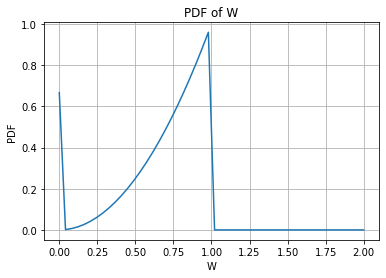
\includegraphics[width=\columnwidth]{solutions/2013/june/70/figures/assignment8pdf.png}
\end{center}
\end{figure}

\begin{figure}[htb!]
\begin{center}
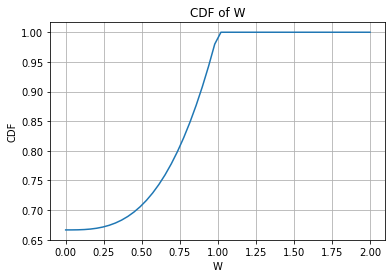
\includegraphics[width=\columnwidth]{solutions/2013/june/70/figures/assignment8cdf.png}
\end{center}
\end{figure}
\end{enumerate}

%
\item Let $U_1,U_2\dots,U_n$ be independent and identically distributed random variables each
having a uniform distribution on (0,1). Then,$\lim_{n \to +\infty} \pr{U_1+U_2\dots,U_n\leq \frac{3}{4}n}$
\begin{enumerate}
    \item does not exist
    \item exists and equals 0
    \item exists and equals 1
    \item exists and equals $\frac{3}{4}$
\end{enumerate}
%
\solution
We use Weak law for large numbers to solve this problem. 
Let the collection of identically distributed random variables $U_1,U_2\dots,U_n$
have a finite mean $\mu$ and finite variance $\sigma^2$.
\begin{align}
    \mu = \mean{U_i} \hspace{0.3cm}\text{for i $\in$ (1,2,3\dots,n)}\label{june2013-59:0.0.1}
\end{align}
Since the distribution is uniform on (0,1), $\mu$ = 0.5. Let $M_n$ be the sample mean
\begin{align}
     M_n = \frac{U_1+U_2+U_3\dots+U_n}{n}\label{june2013-59:0.0.2}
\end{align}
Expected value of $M_n$ (using \eqref{june2013-59:0.0.2} and \eqref{june2013-59:0.0.1})is
\begin{align}
    \mean{M_n} = &\frac{\mean{U_1+U_2+U_3+\dots+U_n}}{\mean{n}}\\[0.3cm]
     = &\frac{\mean{U_1}+\mean{U_2}+\dots+\mean{U_n}}{n}\\
     = &\frac{n\times\mu}{n}\\
     = & \mu
\end{align}
Variance of M
\begin{align}
    Var(M_n) =& \frac{Var(U_1+U_2+U_3\dots+U_n)}{n^2}\\[0.3cm]
    =& \frac{Var(U_1) + Var(U_2)\dots+Var(U_n)}{n^2}\\
    =& \frac{n\times{\sigma^2}}{n^2}\\[0.3cm]
    =& \frac{\sigma^2}{n} \label{june2013-59:0.0.10}
\end{align}
From Chebyshev inequality, for any $\epsilon > 0$
\begin{align}
    \pr{\abs{M_n-\mu}\geq \epsilon} \hspace{0.2cm} \leq \hspace{0.2cm} \frac{Var(M_n)}{\epsilon^2}
\end{align}
From \eqref{june2013-59:0.0.1} and \eqref{june2013-59:0.0.10}
\begin{align}
    \pr{\abs{\frac{U_1+U_2\dots+U_n}{n} - \mu} \geq \epsilon} \leq \frac{\sigma^2}{n\times\epsilon^2}\notag
\end{align}
\begin{align}
    \begin{split}
    \lim_{n \to \infty} \pr{\abs{\frac{U_1+U_2\dots+U_n}{n} - \mu} \geq \epsilon}\\
    \leq \lim_{n \to \infty} \frac{\sigma^2}{n\times\epsilon^2} \leq 0 \hspace{0.2cm} \text{for fixed $\epsilon > 0$}
    \end{split}
\end{align}
But since Probabilities are always non-negative,
\begin{align}
    \lim_{n \to \infty} \pr{\abs{\frac{U_1+U_2\dots+U_n}{n} - \mu} \geq \epsilon} \to 0 \label{june2013-59:0.0.13}
\end{align}
This is known as the weak law of large numbers\\
The inverse of \eqref{june2013-59:0.0.13} is also true
\begin{align}
    &\lim_{n \to \infty} \pr{\abs{\frac{U_1+U_2\dots+U_n}{n} - \mu} \leq \epsilon} \to 1 \\[0.3cm]
    &\abs{\frac{U_1+U_2\dots+U_n}{n} - \mu} \leq \epsilon \hspace{0.2cm}\text{as  n $\to$ $\infty$} 
\end{align}
From $\epsilon$, n definition of limits, it is clear that 
\begin{align}
    &\frac{U_1+U_2\dots+U_n}{n} \to \mu\\
    &U_1+U_2\dots U_n \to n\times\mu \hspace{0.2cm}\text{as  n $\to$ $\infty$}
\end{align}
Since $\mu = \frac{1}{2}$,
\begin{align}
    \lim_{n \to +\infty} U_1+U_2\dots U_n = \frac{1}{2}n < \frac{3}{4}n
\end{align}
So 
\begin{align}
    \lim_{n \to +\infty} \pr{U_1+U_2\dots,U_n\leq \frac{3}{4}n} = 1
\end{align}
%
\item  Consider the quadratic equation $x^2+2U x+V=0$ where $U$ and $V$ are chosen independently and randomly from $\{1,2,3\}$ with equal probabilities. Then probability that the equation has both roots real
\begin{enumerate}
    \item $\frac{2}{3}$
    \item $\frac{1}{2}$
    \item $\frac{7}{9}$
    \item $\frac{1}{3}$
\end{enumerate}
%
\solution
Let $U\in\{1.2,3\}$ and $V\in\{1,2,3\}$
\begin{table}[h!]
\centering
\caption{Probability of selecting values for $U$}
\resizebox{\columnwidth}{!}{
  \begin{tabular}{||c|c|c|c||}
    \hline
    $k$ & $1$ & $2$ & $3$\\
    \hline
    \hline
    $\pr{U=k}$ & $1/3$ & $1/3$ & $1/3$\\
    \hline
  \end{tabular}
}
\label{june2013-60:Table1}
\end{table}
\begin{table}[h!]
\centering
\caption{Probability of selecting values for $V$}
\resizebox{\columnwidth}{!}{
  \begin{tabular}{||c|c|c|c||}
    \hline
    $k$ & $1$ & $2$ & $3$\\
    \hline
    \hline
    $\pr{V=k}$ & $1/3$ & $1/3$ & $1/3$\\
    \hline
  \end{tabular}
}
\label{june2013-60:Table2}
\end{table}
For $x^2+2U x+V=0$ to have real roots,
\begin{align}
    b^2-4ac\geq0\\
    \brak{2U}^2-4\brak{1}\brak{V}\geq0\\
    U^2\geq V
\end{align}
\begin{align}
    \pr{U^2\geq V}=1-\pr{U^2<V}
\end{align}
The possible pairs \brak{U,V} for \pr{U^2<V},
\vspace{0.00001in}
\begin{table}[h!]
\centering
\caption{Table for \pr{U^2<V}}
\resizebox{\columnwidth}{!}{
  \begin{tabular}{||c|c||}
    \hline
    $\brak{U,V}$ for $U^2<V$ & Probability\\
    \hline
    \hline
    $\brak{1,2}$ & \pr{U=1}\pr{V=2}=1/9\\
    \hline
    $\brak{1,3}$ & $\pr{U=1}\pr{V=3}=\frac{1}{9}$\\
    \hline
    \hline
    Total & $\pr{U^2<V}=\frac{2}{9}$\\
    \hline
  \end{tabular}
}
\label{june2013-60:Table3}
\end{table}
\begin{align}
    \pr{U^2\geq V}=1-\frac{2}{9}\\
    \pr{U^2\geq V}=\frac{7}{9}
\end{align}
Hence, Option 3 is correct.

%
\newcommand{\tikzAngleOfLine}{\tikz@AngleOfLine}
  \def\tikz@AngleOfLine(#1)(#2)#3{%
  \pgfmathanglebetweenpoints{%
    \pgfpointanchor{#1}{center}}{%
    \pgfpointanchor{#2}{center}}
  \pgfmathsetmacro{#3}{\pgfmathresult}%
  }

\item A point is chosen at random from a circular disc shown below. What is the probability that the point lies in the sector OAB?\\
\begin{tikzpicture}[
    colorstyle/.style={
       circle, draw=black,fill=black,
       thick, inner sep=0pt, minimum size=2 mm,
       outer sep=0pt
        },
    scale=2]
\draw (0,0) circle (2cm);
\node at (0,0) [colorstyle,label=below:O]{};
\node at (1,1.732) [colorstyle,label=above:A]{};
\node at (1.732,1) [colorstyle,label=above right:B]{};
\draw (0,0) -- (1,1.732);
\draw (0,0) -- (1.732,1);
\coordinate (O) at (0,0);
\coordinate (A) at (1,1.732);
\coordinate (B) at (1.732,1);
\tikzAngleOfLine(O)(B){\AngleStart}
    \tikzAngleOfLine(O)(A){\AngleEnd}
    \draw[red,<->] (O)+(\AngleStart:1cm) arc (\AngleStart:\AngleEnd:1 cm);
    \node[circle,fill=green] at ($(O)+({(\AngleStart+\AngleEnd)/2}:1.5 cm)$) {x};
\end{tikzpicture}\\
( where $\angle$AOB = x radians )
\begin{multicols}{2}
    \begin{enumerate}
        \item $\frac{2x}{\pi}$
        \item $\frac{x}{\pi}$
        \item $\frac{x}{2\pi}$
        \item $\frac{x}{4\pi}$
    \end{enumerate}
\end{multicols}
%
\solution
The joint pdf is given by:
\begin{equation}
 \texorpdfstring{f\textsubscript{r$\theta$}}{f r $\theta$}(r,\theta)= \begin{cases}
                        \dfrac{r}{\pi R^2}  & \text{if 0 $<$ r $<$ R , 0 $<$ $\theta$ $<$ 2$\pi$ }\\
                        0  & \text{otherwise}
                        \end{cases}
\end{equation}
Let A $\equiv$ (R,  $\theta _2$) and B $\equiv$ (R,  $\theta _1$). \\
Hence,
\begin{equation}
(\theta _2 - \theta _1)= x    
\end{equation}
We want $\theta$ $\in$ ($\theta _1$ , $\theta _2$) and r $\in$ (0,R) for point to lie in the sector.
Let the point to be chosen be (r, $\theta$).\\
So, Required probability is:
\begin{align}
 \nonumber  \pr{\theta_1<\theta<\theta_2 , 0<r<R}\\
    =& \Int_{\theta_1}^{\theta_2} \Int_{0}^{R} \dfrac{r}{\pi R^2} \,dr\,d\theta \displaybreak \\
    =& \Int_{\theta_1}^{\theta_2} \dfrac{1}{\pi R^2} \dfrac{r^2}{2} \Bigg|_0^R \\
    =& \Int_{\theta_1}^{\theta_2} \dfrac{R^2}{2\pi R^2} \,d\theta   \\
    =& \Int_{\theta_1}^{\theta_2} \dfrac{1}{2\pi} \,d\theta\\
    =& \dfrac{\theta}{2\pi} \Bigg|_{\theta_1}^{\theta_2} \\
    =& \dfrac{\theta_2 - \theta_1}{2\pi} \\
    =& \dfrac{x}{2\pi}
\end{align}
    
$\therefore$The correct answer is \textbf{option (3)} \Large $\frac{x}{2\pi}$.

%
\item Consider a parallel system with two components. The lifetimes of the two components are independent and identically distributed random variables each following an exponential distribution with mean 1. The expected lifetime of the system is:
\begin{enumerate}[label=\Alph*)]
    \item $1$\\[0.5pt]
    \item $\dfrac{1}{2}$\\
    \item $\dfrac{3}{2}$\\
    \item $2$
\end{enumerate}
%
\solution

Consider two random variables X and Y which represent the lifetime of the two components namely A and B.
\begin{equation}
    X \sim Exp(\lambda_X)
\end{equation}
\begin{equation}
    Y \sim Exp(\lambda_Y)
\end{equation}
% \begin{figure}[h]
%     \centering
%     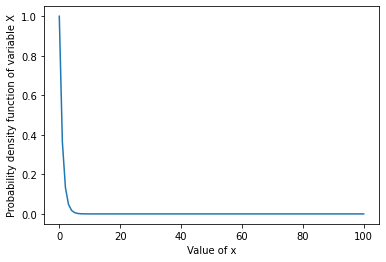
\includegraphics[width=\columnwidth]{solutions/2013/june/42/figures/figure2.png}
%     \caption{P.D.F. of X }
%     \label{june2013-42:june2013-42:fig:fig_label}
% \end{figure}
Let $f_X(x)$ denote the probability distribution function for random variable X.
\begin{align}
f_{X}(x)=
 \begin{cases} 
      \lambda_X  e^{-\lambda_X  x} & x \geq 0 \\
      0 & otherwise
 \end{cases}
\end{align}
Let $f_Y(y)$ denote the probability distribution function for random variable Y.
\begin{align}
f_{Y}(y)=
 \begin{cases} 
      \lambda_Y  e^{-\lambda_Y  y} & y \geq 0 \\
      0 & otherwise
 \end{cases}
 \end{align}
 Let $F_X(x)$ denote the cumulative distribution function for random variable X.
\begin{align}
F_{X}(x)=
 \begin{cases} 
      1-e^{-\lambda_X  x} & x \geq 0 \\
      0 & otherwise
 \end{cases}
\end{align}
Let $F_Y(y)$ denote the cumulative distribution function for random variable Y.
\begin{align}
F_{Y}(y)=
 \begin{cases} 
      1-e^{-\lambda_Y  y} & y \geq 0 \\
      0 & otherwise
 \end{cases}
 \end{align}
\begin{equation}\label{june2013-42:meanx}
    E(X)=\dfrac{1}{\lambda_X}
\end{equation}
\begin{equation}\label{june2013-42:meany}
    E(Y)=\dfrac{1}{\lambda_Y}
\end{equation}
From \ref{june2013-42:meanx} and \ref{june2013-42:meany},
\begin{equation}\label{june2013-42:lambda}
    \lambda_X = \lambda_Y = 1
\end{equation}
\begin{figure}[h]
    \centering
    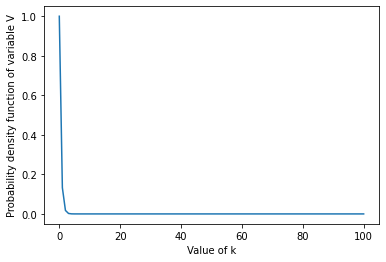
\includegraphics[width=\columnwidth]{solutions/2013/june/42/figures/figure.png}
    \caption{Parallel system}
    \label{june2013-42:fig:fig_label}
\end{figure}
Let Z be a random variable such that $Z=max(X,Y)$
\begin{align}
    P(Z\leq z) &= P(max(X,Y) \leq z)
    \\
    &=P(X\leq z,Y\leq z)
    \\
    &=P(X\leq z) P(Y\leq z)
    \\
    &=(F_X(z)-F_X(0)) (F_Y(z)-F_Y(0))
    \\
    &=1-e^{-(\lambda_X) z}-e^{-(\lambda_Y) z}+e^{-(\lambda_X+\lambda_Y) z}
\end{align}
$P(Z\leq z)$ denotes the probability that the system dies in the first $z$ seconds.\\
\begin{align}
    Expectation &= \int_{0}^{\infty}z \,d(P(Z\leq z))
    \\
\nonumber    &=\int_{0}^{\infty}z(\lambda_Xe^{-(\lambda_X) z}+\lambda_Ye^{-(\lambda_Y) z}\\
&-(\lambda_X+\lambda_Y)e^{-(\lambda_X+\lambda_Y) z}) \,dz
    \\
    &= \dfrac{1}{\lambda_X}+\dfrac{1}{\lambda_Y}-\dfrac{1}{\lambda_X+\lambda_Y}
\end{align}
From \ref{june2013-42:lambda}, 
\begin{equation}
    Expectation=\dfrac{3}{2}
\end{equation}
Therefore, option C correct.

%
\item Let $X_1$,$X_2$,... be independent random variables each following exponential distribution with mean 1. Then which of the following statements are correct?
\begin{enumerate}
    \item P($X_n > \log n$ for infinitely many $n \geq 1$) = 1
    \item P($X_n > 2$ for infinitely many $n \geq 1$) = 1
    \item P($X_n > \frac{1}{2}$ for infinitely many $n \geq 1$) = 0
    \item P($X_n > \log n, X_{n+1}>\log (n+1)$ for infinitely many $n \geq 1$) = 0
\end{enumerate}
%
\solution
\newcommand{\Integral}[2]{\ensuremath{\int\limits_{#1}^{#2}}}
PDF of $X_i$ is
\begin{align}
    f_{X_i}(x)=\begin{cases}\lambda_i e^{-\lambda_i x}, &x\geq 0\\
                0, &x<0\nonumber
    \end{cases}    
\end{align} 
Mean of $X_i$ is expressed as
\begin{align}
    \mean{X_i}&=\Integral{-\infty}{\infty}x f_{X_i}(x) dx\nonumber\\
              &=\Integral{-\infty}{0}0 dx + \Integral{0}{\infty}x \lambda_i e^{-\lambda_i x}\nonumber\\
              &=\frac{1}{\lambda_i}\label{june/2013/101a}
\end{align}
From \eqref{june/2013/101a}and $\mean{X_i}=1$, we have $\lambda_i=1 \forall  i \geq1$
Now, for some constant $c\geq0$
\begin{align}
    \pr{X_n>c}&=\Integral{c}{\infty}f_{X_n}(x)dx\nonumber\\
              &=\Integral{c}{\infty}e^{-x}dx\nonumber\\
              %&=-e^{-x}\Big|_c^{\infty}\nonumber\\
              &=e^{-c}\label{june/2013/101b}
\end{align}
\textbf{Borel-Cantelli Lemma}:\\
Let $E_1$,$E_2$,... be a sequence of events in some probability space. The Borel–Cantelli lemma states that, if the sum of the probabilities of the events $E_n$ is finite
\begin{align}
    \sum_{n=1}^{\infty}\pr{E_n}&<\infty
\end{align}
then the probability that infinitely many of them occur is 0
\begin{align}
    \pr{\lim_{n \rightarrow \infty}\sup E_n}&=0
\end{align}
\textbf{Second Borel-Cantelli Lemma}:\\
If the events $E_n$ are independent and the sum of the probabilities of the $E_n$ diverges to infinity, then the probability that infinitely many of them occur is 1.
If for independent events $E_1,E_2,...$
\begin{align}
    \sum_{n=1}^{\infty}\pr{E_n}&=\infty
\end{align}
Then
\begin{align}
    \pr{\lim_{n \rightarrow \infty}\sup E_n}&=1
\end{align}
\bigskip
\begin{enumerate}
    \item \textbf{Option 1:} 
    We can say the events $X_n>\log n$ are independent $\forall n\geq 1$ as $X_n$ are independent random variable.
    
    From \eqref{june/2013/101b}
    \begin{align}
        \sum_{n=1}^{\infty}\pr{X_n > \log n} &=\sum_{n=1}^{\infty}e^{-\log n}\nonumber\\ &=\sum_{n=1}^{\infty}\frac{1}{n}\nonumber\\
                                            &= \infty  \text{ (Cauchy's Criterion)}\nonumber
    \end{align}
    Now, from second Borel-Cantelli lemma
    \begin{align}
        &\pr{X_n>\log n \text{ for infinitely many }n\geq1}\nonumber\\
        &=\pr{\lim_{n \rightarrow \infty}\sup X_n>\log n}\nonumber\\
        &=1\nonumber
    \end{align}
    $\therefore$ Option 1 is correct. 
    
    \item\textbf{Option 2:} We can say the events $X_n>2$ are independent $\forall n\geq 1$ as $X_n$ are independent random variable.
    
    From \eqref{june/2013/101b}
    \begin{align}
        \sum_{n=1}^{\infty}\pr{X_n > 2} &= \sum_{n=1}^{\infty}e^{-2}\nonumber\\
                                            &= \infty\nonumber
    \end{align}
    Now, from second Borel-Cantelli lemma
    \begin{align}
        &\pr{X_n>2 \text{ for infinitely many }n\geq1}\nonumber\\
        &=\pr{\lim_{n \rightarrow \infty}\sup X_n>2}\nonumber\\
        &=1\nonumber
    \end{align}
    $\therefore$ Option 2 is correct.
    
    \item \textbf{Option 3:} We can say the events $X_n>\frac{1}{2}$ are independent $\forall n\geq 1$ as $X_n$ are independent random variable.
    
    From \eqref{june/2013/101b}
    \begin{align}
        \sum_{n=1}^{\infty}\pr{X_n > \frac{1}{2}} &= \sum_{n=1}^{\infty}e^{-\frac{1}{2}}\nonumber\\
                                            &= \infty\nonumber
    \end{align}
    Now, from second Borel-Cantelli lemma
    \begin{align}
        &\pr{X_n>\frac{1}{2} \text{ for infinitely many }n\geq1}\nonumber\\
        &=\pr{\lim_{n \rightarrow \infty}\sup X_n>\frac{1}{2}}\nonumber\\
        &=1\nonumber
    \end{align}
    $\therefore$ Option 3 is incorrect.
    \item \textbf{Option 4:} We can say the events $X_n>\log n$ are independent $\forall n\geq 1$ as $X_n$ are independent random variable.
    
    Let the event $X_n > \log n,X_{n+1}>\log (n+1)$ be represented by $E_n$'
    
    From \eqref{june/2013/101b}
    \begin{align}
        &\sum_{n=1}^{\infty}\pr{E_n}\nonumber\\
        &= \sum_{n=1}^{\infty}\pr{X_n>\log n}\pr{X_{n+1}>\log (n+1)}\nonumber\\
        &=\sum_{n=1}^{\infty}e^{-\log n}e^{-\log (n+1)}\nonumber\\
        &=\sum_{n=1}^{\infty}\frac{1}{n(n+1)}\nonumber\\
        &=\sum_{n=1}^{\infty}\frac{1}{n}-\frac{1}{n+1}\nonumber\\
        &=1
    \end{align}
    Now, from Borel-Cantelli lemma
    \begin{align}
        &\pr{E_n\text{ for infinitely many }n\geq1}\nonumber\\
        &=\pr{\lim_{n \rightarrow \infty}\sup ( X_n>\log n,X_{n+1}>\log (n+1))}\nonumber\\
        &=0\nonumber
    \end{align}
    $\therefore$ Option 4 is correct.
\end{enumerate}
\vspace{0.5cm}\centering \boxed{\solution{\text{Options 1, 2, 4}}}
%


\end{enumerate}


% \section{December 2012}
% \renewcommand{\theequation}{\theenumi}
\renewcommand{\thefigure}{\theenumi}
\renewcommand{\thetable}{\theenumi}
\begin{enumerate}[label=\thesection.\arabic*.,ref=\thesection.\theenumi]
\numberwithin{equation}{enumi}
\numberwithin{figure}{enumi}
\numberwithin{table}{enumi}

\item Let X be a binomial random variable with parameters  $\brak{11,\displaystyle{\frac{1}{3}}}$. At which value(s) of k is $\Pr\brak{X = k}$ maximized?\\
\begin{enumerate}
\item k=2
\item k=3
\item k=4
\item k=5
\end{enumerate}
%
\solution
X has a binomial distribution :
\begin{align}
\Pr\brak{X=k} = {\comb{n}{k}}(q)^{n-k}(p)^{k}
\end{align}
Where,
\begin{itemize}
\item n=11
\item $\displaystyle{p=\frac{1}{3}}$
\item $\displaystyle{q=1-p=1-\frac{1}{3}=\frac{2}{3}}$
\end{itemize}
\begin{align}
\Pr\brak{X = k}={\comb{11}{k}}\left(\frac{2}{3}\right)^{11-k}\left(\frac{1}{3}\right)^{k}
\end{align}
For Pr(X = k) to be maximized
\begin{align}
\Pr\brak{X = k}\:\geq\:\Pr\brak{X = k+1}\\
\frac{\Pr\brak{X = k}}{\Pr\brak{X = k+1}}=\frac{{\comb{11}{k}}\left(\frac{2}{3}\right)^{11-k}\left(\frac{1}{3}\right)^{k}}{{\comb{11}{k+1}}\left(\frac{2}{3}\right)^{10-k}\left(\frac{1}{3}\right)^{k+1}}\geq1
\end{align}
\begin{align}
\frac{2(k+1)}{11-k}\geq1\\
\implies k\geq3\label{dec2012-104:0.0.7}\\
\Pr\brak{X = k}\:\geq\:\Pr\brak{X = k-1}\\
\frac{\Pr\brak{X = k}}{\Pr\brak{X = k-1}}=\frac{{\comb{11}{k}}\left(\frac{2}{3}\right)^{11-k}\left(\frac{1}{3}\right)^{k}}{{\comb{11}{k-1}}\left(\frac{2}{3}\right)^{12-k}\left(\frac{1}{3}\right)^{k-1}}\geq1\\
\frac{12-k}{2k}\geq1\\
\implies k\leq4\label{dec2012-104:0.0.10}
\end{align}
From \eqref{dec2012-104:0.0.7} , \eqref{dec2012-104:0.0.10} and since k is an integer\\
$\Pr\brak{X = k}$ is maximized for k=3, k=4\\
Thus options 2) and 3) are correct\\

\end{enumerate}

% \section{June 2012}
% \renewcommand{\theequation}{\theenumi}
\renewcommand{\thefigure}{\theenumi}
\renewcommand{\thetable}{\theenumi}
\begin{enumerate}[label=\thesection.\arabic*.,ref=\thesection.\theenumi]
\numberwithin{equation}{enumi}
\numberwithin{figure}{enumi}
\numberwithin{table}{enumi}

\item Let $X_1,X_2,X_3,....,X_n$ be i.i.d observations from a distribution with continuous probability density function f which is symmetric around $\theta$ i.e
\begin{align}
    f\brak{x-\theta}=f\brak{\theta -x}
\end{align}
for all real x.Consider the test $H_0: \theta =0$ vs $H_1:  \theta >0$ and the sign test statistic
\begin{align}
    S_n = \sum_{i=1}^{n} sign(X_i)
\end{align}
where
\begin{align}
    sign(x) =
    \begin{cases}
    1  & x>0\\
    0  & x=0\\
    -1 & x<0
    \end{cases}
\end{align}
Let $z_\alpha$ be the upper $100(1-\alpha)^{th}$ percentile of the standard normal distribution where $0<\alpha <1$. Which of the following is/are correct?
\begin{enumerate}
    \item If $\theta =0$ then $ \lim_{n\to\infty} P\cbrak{S_n > \sqrt{n}z_{\alpha}} =1 $\\
    \item If $\theta =0$ then $ \lim_{n\to\infty} P\cbrak{S_n > \sqrt{n}z_{\alpha}} =\alpha $\\
    \item If $\theta >0$ then $ \lim_{n\to\infty} P\cbrak{S_n > \sqrt{n}z_{\alpha}} = 1 $\\
    \item If $\theta >0$ then $ \lim_{n\to\infty} P\cbrak{S_n > \sqrt{n}z_{\alpha}} =\alpha $
\end{enumerate}
%
\solution
{$H_0:\theta=0$}
Assume hypothesis
$H_0:\theta=0$ is true.
\begin{enumerate}
\item Given X is symmetric around zero.
 \begin{align}
  f_X(x)&=f_X(-x)\\
  \int_{0}^{\infty}f_X(x)dx&=\int_{0}^{\infty}f_X(-x)dx
  \label{june/2012/112/int}
\end{align}
\begin{enumerate}
\item Solving LHS of $\eqref{june/2012/112/int}$
\begin{align}
    \int_{0}^{\infty}f_X(x)dx=\pr{X\geq0}
\end{align}
\item Solving RHS of $\eqref{june/2012/112/int}$
\begin{align}
    \int_{0}^{\infty}f_X(-x)dx
\end{align}
Changing $-x \rightarrow x$ we get 
\begin{align}
  \int_{0}^{\infty}f_X(-x)dx&=\int_{-\infty}^{0}f_X(x)dx\label{june/2012/112/rhs}\\
  &=\pr{X\leq0}
\end{align}
\end{enumerate}
but
\begin{align}
  \int_{-\infty}^{0}f_X(x)dx+\int_{0}^{\infty}f_X(x)dx=1
  \label{june/2012/112/pr}
\end{align}
from $\eqref{june/2012/112/int}$ , $\eqref{june/2012/112/rhs}$ and $\eqref{june/2012/112/pr}$
\begin{align}
\int_{-\infty}^{0}f_X(x)dx=\int_{0}^{\infty}f_X(x)dx=\frac{1}{2}
\end{align}
\begin{align}
    \implies \pr{X\leq 0}=\pr{X\geq0}=\frac{1}{2}
    \label{june/2012/112/sym}
\end{align}
\item Let Y be a random variable such that
\begin{align}
    Y=sign(X)
\end{align}
\begin{align}
    Y=
    \begin{cases}
     1 & X>0\\
    -1 & X<0
    \end{cases}
    \label{june/2012/112/t}
\end{align}
From $\eqref{june/2012/112/sym}$ and $\eqref{june/2012/112/t}$
we have
\begin{align}
   \pr{Y=-1}=\pr{Y=1}=\frac{1}{2} 
\end{align}
So $Y=sign(X)$ is also symmetric around zero.
% \begin{figure}[!ht]
% \centering
% 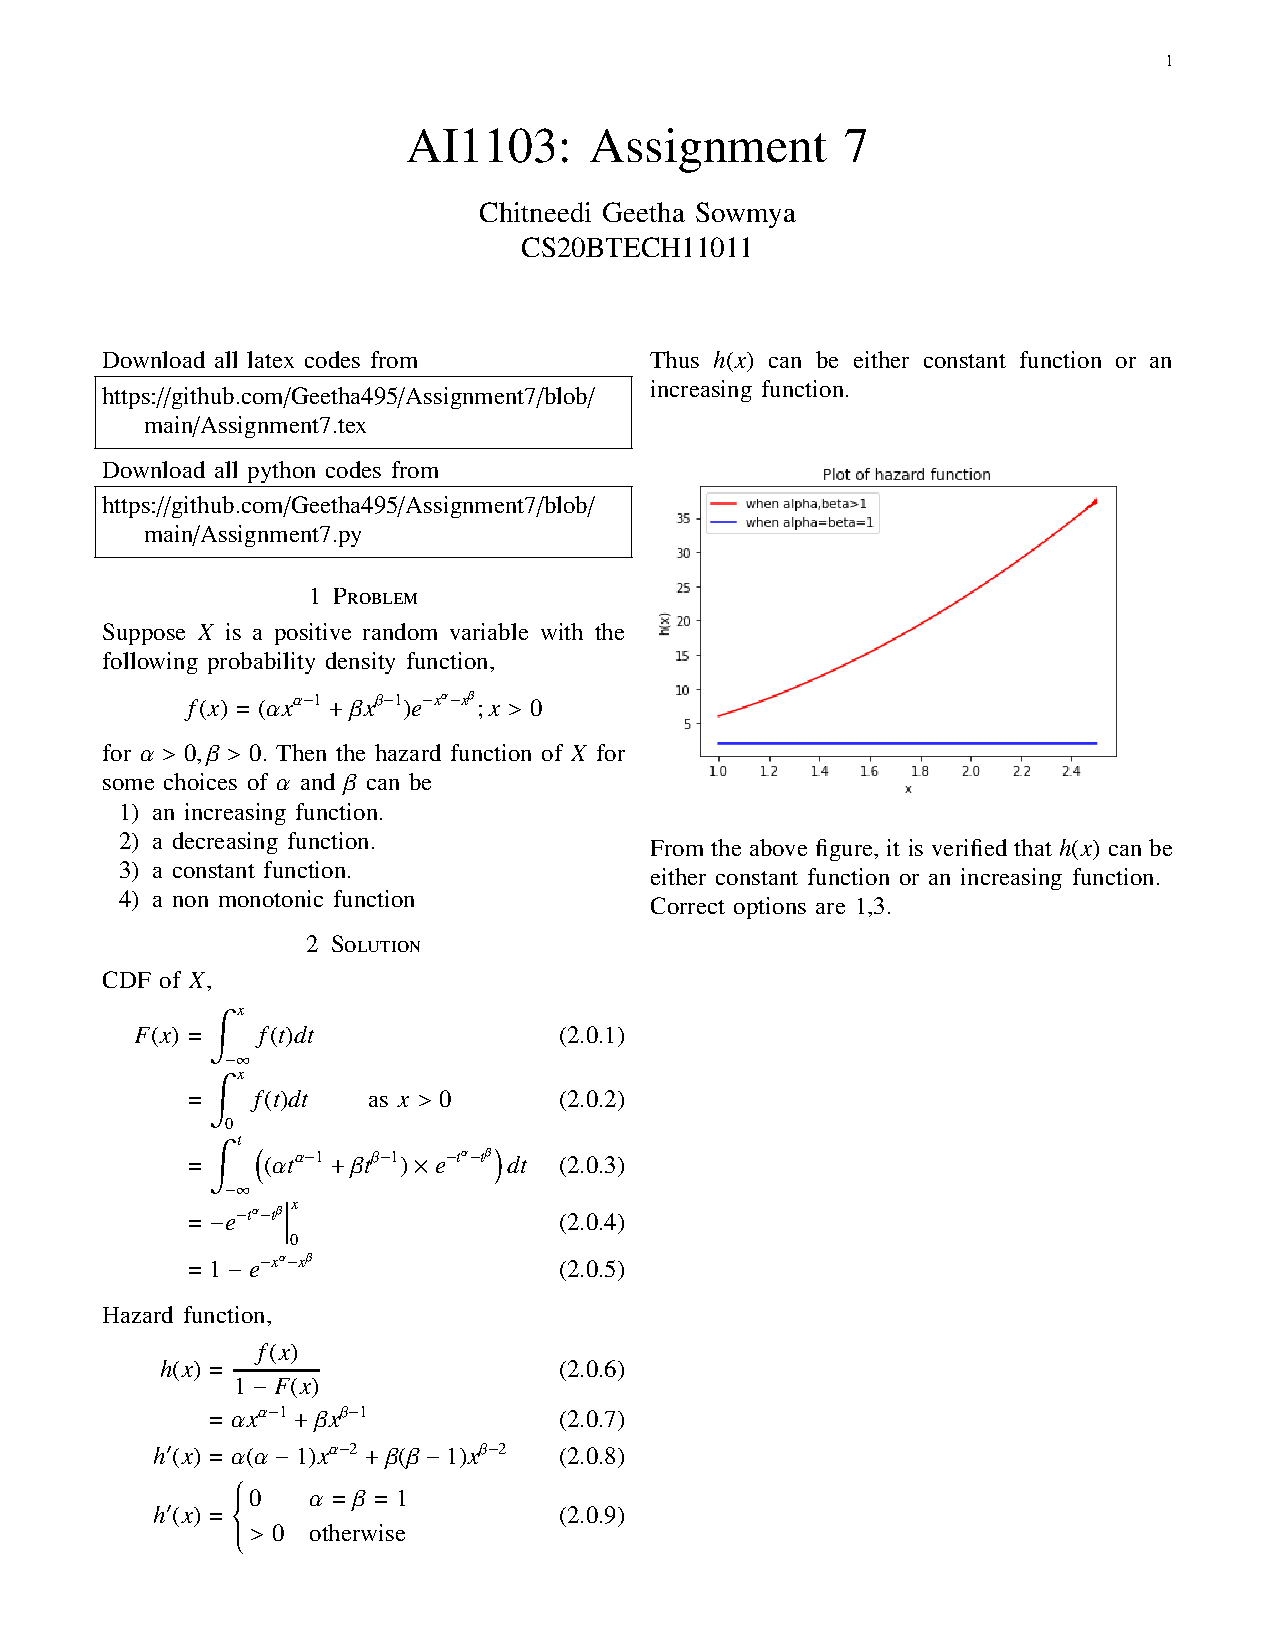
\includegraphics[width=\columnwidth]{Assignment7.png}
% \caption{pdf of $ Y=sign(X)$}
% \label{june/2012/112/pdf}
% \end{figure}
\begin{align}
   \implies \mu_y = 0 
\end{align}
and variance is
\begin{align}
    \sigma_y^2 &= (-1)^2\brak{\frac{1}{2}}+(1)^2\brak{\frac{1}{2}}\\
    &=1
\end{align}
\item Given
\begin{align}
    S_n&=\sum_{i=1}^{n} sign(X_i)\\
    S_n(\theta=0)&=\sum_{i=1}^{n} Y_i
\end{align}
From central limit theorem 
\begin{align}
    Z&=\lim_{n\to\infty}\sqrt{n}\brak{\frac{\frac{S_n}{n}-\mu_y}{\sigma_y}}\\
    &=\lim_{n\to\infty}\sqrt{n}\brak{\frac{S_n}{n}}\\
    &=\lim_{n\to\infty}\brak{\frac{S_n}{\sqrt{n}}}
    \label{june/2012/112/clt}
\end{align}
where Z is a standard normal variable N(0,1).
\begin{enumerate}
    \item Given
\begin{align}
    \alpha = P\cbrak{Z>z_\alpha}\label{june/2012/112/uff}
\end{align}
So from $\eqref{june/2012/112/clt}$ and $\eqref{june/2012/112/uff}$
\begin{align}
\lim_{n\to\infty}P\cbrak{\frac{S_n}{\sqrt{n}}>z_\alpha}&=
\alpha\\
\implies \lim_{n\to\infty}P\cbrak{S_n>\sqrt{n}z_\alpha}&=
\alpha
\end{align}
\end{enumerate}
\end{enumerate}
{$H_1:\theta >0$ is true}
\begin{enumerate}
    \item Given X is symmetric around $\theta>0$.Let us assume $\theta=\theta_0>0$.
    \begin{align}
        f_X(\theta_0-x)&=f_X(\theta_0+x)\\
        \int_{\theta_0}^{\infty} f_X(\theta_0-x)dx&=
        \int_{\theta_0}^{\infty} f_X(\theta_0+x)dx
        \label{june/2012/112/s}
    \end{align}
    \begin{enumerate}
        \item Solving LHS of $\eqref{june/2012/112/s}$.Changinng $(\theta_0-x) \rightarrow t$
        \begin{align}
           \int_{\theta_0}^{\infty} f_X(\theta_0-x)dx&=
           \int_{-\infty}^{0}f_X(t) dt\\
           &=\pr{X\leq0}\label{june/2012/112/temp}
        \end{align}
        \item Solving RHS of $\eqref{june/2012/112/s}$.Changing $(\theta_0+x) \rightarrow t$
        \begin{align}
           \int_{\theta_0}^{\infty} f_X(\theta_0+x)dx&=
           \int_{2\theta_0}^{\infty} f_X(t)dt\\
          &= \int_{0}^{\infty} f_X(t)dt-\int_{0}^{2\theta_0} f_X(t)dt\\
          &=\pr{X\geq0}-k\label{june/2012/112/u}
        \end{align}
        where
        \begin{align}
           k=\int_{0}^{2\theta_0} f_X(t)dt>0 
        \end{align}
    \end{enumerate}
    From $\eqref{june/2012/112/s}$,$\eqref{june/2012/112/t}$ and $\eqref{june/2012/112/u}$
    \begin{align}
        \pr{X\geq0}>\pr{X\leq0}
    \end{align}
    \item So
    \begin{align}
        \pr{Y=1}>\pr{Y=-1}
    \end{align}
    Therefore,if we perform the experiment and find the value of $\brak{\frac{S_n}{\sqrt{n}}}$,it is most likely to occur on the right side of the distribution of 
$\brak{\frac{S_n}{\sqrt{n}}}$.In $\eqref{june/2012/112/clt}$ it is shown that distrubution of the random variable $\brak{\frac{S_n}{\sqrt{n}}}$
 is $N(0,1)$ when n is very large.So
\begin{align}
    \lim_{n\to\infty}P\cbrak{\frac{S_n}{\sqrt{n}}>Z_\alpha}=1
\end{align}
\end{enumerate}

\end{enumerate}


\end{document}


